\documentclass[12pt]{report}  
%
\bibliographystyle{elsevier}      
\usepackage{epsfig}
\usepackage{fancyhdr}
\usepackage{bm}
\input epsf
\usepackage[dvips]{color}
\usepackage{lscape}
\usepackage{longtable}
\usepackage{hhline}
\usepackage{alltt}
\usepackage{ifthen}
\usepackage{amsmath}
\usepackage{tabularx}
\usepackage{latexsym}

\topmargin -0.5 in
\headheight 0.0in
\headsep 0.5in
\textheight 9.0in
\oddsidemargin -.0in
\evensidemargin -.0in
\textwidth 6.6in

\def\beqn{\begin{eqnarray}}
\def\eeqn{\end{eqnarray}}
\def\beq{\begin{equation}}
\def\eeq{\end{equation}}
\def\1035{10$^{35}$~cm$^{-2}$s$^{-1}$}
\def\degg{$^{\circ}$ }
\def\qsq{$Q^2 $}
\def\co2{$CO_2 $}
\def\microns{$\mu m $}
\def\gevcsq{$GeV/c^2 $}
\def\gev{$GeV $}
\def\gevc{$GeV/c $}

%
\newcommand{\la}{\langle}
\newcommand{\ra}{\rangle}
\newcommand{\zh}{z}
\newcommand{\xbj}{x_{\scriptscriptstyle B}}
%
\newcommand{\Epgb}{$\vec ep \to ep(p,\Delta, N^*)\gamma~$}
\newcommand{\Epgl}{$\vec e\vec p \to ep(p,\Delta, N^*)\gamma~$}
\newcommand{\Epgt}{$ep^T \to ep(p,\Delta, N^*)\gamma~$}
\newcommand{\Thgg}{$\theta_{\gamma^*\gamma}~$}
\newcommand{\Phgg}{$\phi_{\gamma^*\gamma}~$}
\newcommand{\Epg}{$ep \to ep\gamma~$}
\newcommand{\Eppiz}{$ep \to ep\pi^0~$}
\newcommand{\Enpip}{$ep \to en\pi^+~$}
\newcommand{\EppiD}{$ep \to e\pi \Delta~$}
\newcommand{\Epeta}{$ep \to ep\eta~$}
\newcommand{\Epr}{$ep \to ep\rho~$}
\newcommand{\EpX}{$ep \to epX~$}
\newcommand{\EpKY}{$ep \to eKY~$}
\newcommand{\vEpg}{$\vec ep \to ep\gamma~$}
\newcommand{\xidef}{$\xi=x_B\frac{1+\frac{Delta^2}{2Q^2}}{2-x_B+x_B\frac{Delta^2}{2Q^2}}$}
\def\gevc2{(GeV/c)$^2$}
\newcommand{\EpgX}{$ep \to ep\gamma X~$}
\newcommand{\bfk}{\mbox{\boldmath $k$}}
\newcommand{\bfP}{\mbox{\boldmath $P$}}
\newcommand{\bfp}{\mbox{\boldmath $p$}}
\def\VEC#1{\hbox{\boldmath$#1$\unboldmath}}
\def\Vec#1{{\bf #1}}
\def\slash{/\!\!\!}
\def\one{1 \!\! 1}
\def\D{{\mathrm d}}
\def\E{{\mathrm e}}
\def\I{{\mathrm i}}
\renewcommand{\baselinestretch}{1.4}
\title{CLAS12 Technical Design Report \\
\Large Version 5.1}

\date{\today}
\begin{document}
%
%\thispagestyle{empty}
%\begin{figure}[htbp]
%\vspace{20.0cm}
%\special{psfile=TDRcover.ps hscale=95 vscale=95 hoffset=-55 voffset=-90}
%\end{figure}

%\pagebreak
%\clearpage

%\thispagestyle{empty}
%~~

%\newpage

%\thispagestyle{empty}

%\pagenumbering{arabic}	
\maketitle

\thispagestyle{empty}
\vspace{2cm}
\newpage
\thispagestyle{empty}

~~
\vfil
\eject

\noindent
{\bf \large \underline{Participating Institutions:}}\\ 

\vspace{0.3cm}

\noindent 
Arizona State University, Tempe, AZ\\
Argonne National Laboratory, Argonne, IL\\
California State University, Dominguez Hills, CA\\
Catholic University of America, Washington, DC\\
CEA-Saclay,  Gif-sur-Yvette, France\\
University of Connecticut, Storrs, CT\\
Edinburgh University, Edinburgh, UK\\
Fairfield University, Fairfield, CT\\
Florida International University, Miami, FL\\
University of Glasgow, Glasgow, UK\\
Hampton, University, Hampton, VA\\
Idaho State University, Pocatello, Idaho\\
INFN, Laboratori Nazionali di Frascati, Fascati, Italy\\
INFN, Sezione di Genova, Genova, Italy\\
Institute of Theoretical and Experimental Physics (ITEP), Moscow, Russia\\
James Madison University, Harrisonburg, VA\\
Kyungpook University, Daegu, South Korea\\
Los Alamos National Laboratory, Los Alamos, NM\\
Moscow State University, Moscow, Russia\\
University of New Hampshire, Durham, NH\\
Norfolk State University, Norfolk, VA\\
Ohio University, Athens, OH\\
Old Dominion University, Norfolk, VA\\
Institut de Physique Nucleaire, Orsay, France\\
Rensselaer Polytechnic Institute, Troy, NY\\
Rice University, Houston, TX\\
University of Richmond, Richmond, VA\\
University of South Carolina, Columbia, SC\\
Temple University, Philadelphia, PA\\
Thomas Jefferson National Accelerator Facility, Newport News, VA\\
Virginia Polytechnic Institute and State University, Blacksburg, VA\\
University of Virginia, Charlottesville, VA\\
College of William and Mary, Williamsburg, VA\\
Yerevan Institute of Physics, Yerevan, Armenia\\

\newpage
\thispagestyle{empty}

~~
\vfil
\eject

\tableofcontents

\newpage

\fancypagestyle{myheading}{%                % Redefining plain style
\fancyhf{} % clear all header and footer fields
\fancyhead[C]{\vspace{0.5cm}\line(1,0){500}\vspace{-0.5cm}}
\fancyhead[l]{\mbox{\bfseries The CLAS12 Physics Program}}
\fancyhead[r]{\mbox{\bfseries Version 5.1  \date{\today}}}
\fancyfoot[C]{\mbox{\bfseries  \thepage }}
\fancyfoot[r]{\mbox{\bfseries Physics Program}}
\fancyfoot[l]{\vspace{-1cm}\line(1,0){500}}
}
\renewcommand{\headrulewidth}{0pt}
\renewcommand{\footrulewidth}{0pt}
\pagestyle{myheading}
\vspace{5cm}

%
%%%%%%%%%%%%%%%%%%%%%%%%%%%%%%%%%%%%%%%%%%%%%%%%%%%%%%%%%%%%%%%%%%%%%%%%
%

\part{Physics}

\setcounter{chapter}{0}
\setcounter{section}{0}
\setcounter{subsection}{1}

%%%%%%%%%%%%%%%%%%%%%%%%%%%%%%%%%%%%%%%%%%%%%%%%%%%%%%%%%%%%%%%%%%%%%%%%

\chapter{Executive Summary}

In the past five decades many important discoveries have been made  
in electron-proton scattering experiments.  The finite size of the 
proton was measured in Hofstadter's pioneering experiment in which 
electrons of 188~MeV energy were elastically scattered off a hydrogen 
target~\cite{hofstadter}.  It demonstrated conclusively that the proton 
is not a Dirac particle but has a finite size. Hofstadter was awarded 
the Nobel prize in 1961 for this discovery.  The energy of Hofstadter's 
accelerator was not high enough to resolve the internal structure of the 
proton but it laid the groundwork for a vigorous research program of 
inclusive electron scattering.  It took another decade, and the 
construction of the powerful electron accelerator and the large magnetic 
spectrometers at the Stanford Linear Accelerator Center (SLAC), to ``see'' 
deep into the proton's interior.  At energies of 20~GeV, experimental 
groups led by Jerome Friedman, Henry Kendall, and Richard Taylor discovered 
``scaling'', i.e. the independence of deeply inelastic structure functions 
of the proton on the virtuality of the electromagnetic probe
\cite{scaling, scaling2}.  These results could only be interpreted in 
terms of electron scattering off point-like ``partons'' inside the proton. 
They were also a triumph for the quarks postulated earlier by theorists 
Murray Gell-Mann~\cite{gellmann} and George Zweig~\cite{zweig} as the 
fundamental building blocks for hadrons.  Gell-Mann received the Nobel 
prize in 1969. For the experimental discovery of the proton's quark structure 
Friedman, Kendall, and Taylor shared the Nobel prize in 1990.  The small 
but significant deviations from scaling that were observed in the SLAC 
experiments also had significant impact on the development of the theory 
of Quantum Chromodynamics (QCD), and are fully explained by the emission 
of gluons from the struck quarks. 

Deeply Inelastic Scattering (DIS) experiments, where only the scattered 
electron is detected, have been carried out up to the highest energies at 
CERN and at DESY. The longitudinal momentum and spin densities of the
quarks have been mapped out in detail.  We have also learned that the 
quarks are not the only tenants of the proton, but that more than 50\% of 
the momentum of the proton is carried by the glue needed to bind the quarks 
together.  More recently, inclusive polarized electron scattering off 
polarized protons led to the ``spin puzzle'', the finding that the quark 
spin contributes less than 25\% of the total spin of the proton, leaving 
much to be understood about the origin of spin~\cite{filipone}.  DIS 
experiments will continue to play an important role in further unraveling 
the valence quark structure, especially under extreme conditions, e.g. 
when one quark carries nearly the full proton momentum.

%%%%%%%%%%%%%%%%%%%%%%%%%%%%%%%%%%%%%%%%%%%%%%%%%%%%%%%%%%%%%%%%%%%%%%%%%
\begin{figure}[htbp]
\vspace{7.7cm} 
\special{psfile=handbag_GPD.ps hscale=33 vscale=33 hoffset=140 voffset=-15}
\caption{\small{The ``handbag'' diagrams for deeply virtual Compton 
scattering (a), and for deeply virtual meson production (b).  Four GPDs 
describe the ``soft'' proton structure part.  They depend not only on $x$, 
but on two more variables: the momentum imbalance of the quark before and 
after the interaction, $\xi$, and the momentum transfer to the proton, $t$.}}
\label{hand_bag}
\end{figure}
%%%%%%%%%%%%%%%%%%%%%%%%%%%%%%%%%%%%%%%%%%%%%%%%%%%%%%%%%%%%%%%%%%%%%%%%%

A glorious past and present is a good basis but not a guarantee for a 
successful future. So, what is the new physics that we are confident will 
shape the future of nuclear physics with electromagnetic probes for the 
coming decades?  While the major discoveries in electromagnetic physics 
have so far come from electron scattering experiments where only the 
scattered electron is measured in magnetic spectrometers, in particular 
measurement of elastic form factors and longitudinal parton densities, they 
are not sufficient to unravel the full structure and internal dynamics of 
the proton.  Semi-exclusive measurements, in which one hadron is observed 
in addition to the scattered electron, are needed to study its flavor 
structure, and only fully exclusive processes in which all final products 
are reconstructed can unravel the complete internal dynamics of the proton.
The experimental and theoretical tools for such an endeavor are now on the 
horizon: electron machines such as CEBAF at 12~GeV, with its CW beams 
and large acceptance detectors operating at high luminosities, are needed 
for the experimental part of such a program, while the new formalism of 
Generalized Parton Distributions (GPDs) provides the theoretical framework 
for the interpretation of the new experiments
\cite{mueller,Ji97_1,Ji97_2,Radyushkin:1996nd,Radyushkin:1997ki}.  The basis 
for this approach are the ``handbag'' diagrams shown in Fig.~\ref{hand_bag}.
Here the electron knocks a quark out of the proton by exchanging a deeply 
virtual (massive) photon. The quark then emits a high energy photon (a) and 
is put back into the proton. Alternatively, a $q\bar q$ pair (meson) is 
created, and one of the quarks is returned into the proton (b).   At 
sufficiently high energies and high virtuality of the exchanged photon 
(``Bjorken regime'') these processes are controlled by perturbative QCD, and 
the results can be interpreted in terms of ``soft'' correlation functions, the 
GPDs. They describe the full complexity of the proton's structure and 
dynamics.        

%%%%%%%%%%%%%%%%%%%%%%%%%%%%%%%%%%%%%%%%%%%%%%%%%%%%%%%%%%%%%%%%%%%%%%%%%
\begin{figure}[ht]
\vspace{8.5cm} 
\special{psfile=fig02-1.ps hscale=50 vscale=50 hoffset=-60 voffset=-55}
\special{psfile=fig02-2.ps hscale=50 vscale=50 hoffset=85 voffset=-58}
\special{psfile=fig02-3.ps hscale=50 vscale=50 hoffset=230 voffset=-65}
\caption{\small{Representations of the proton properties probed in elastic 
scattering (left), deeply inelastic scattering (center), and deeply 
exclusive scattering processes (right). Elastic scattering measures the 
charge density $\rho (b_{\perp})$ as a function of the impact parameter 
$b_{\perp}$.  DIS measures the longitudinal parton momentum fraction density 
$f(x)$. GPDs measure the full correlation function $f(x,b_{\perp},\xi)$ where 
$\xi$ represents the longitudinal momentum imbalance of the struck quark 
before and after the interaction. The graph shows the correlation function 
at $\xi=0$.}}
\label{fig:figure1}
\end{figure}
%%%%%%%%%%%%%%%%%%%%%%%%%%%%%%%%%%%%%%%%%%%%%%%%%%%%%%%%%%%%%%%%%%%%%%%%%

%%%%%%%%%%%%%%%%%%%%%%%%%%%%%%%%%%%%%%%%%%%%%%%%%%%%%%%%%%%%%%%%%%%%%%%%%
\begin{figure}[ht]
\vspace{11.0cm} 
\special{psfile=mb-dgpd.eps hscale=55 vscale=55 hoffset=70 voffset=-70}
\caption{\small{Simulated proton tomography images for the $d$-quarks, 
showing the strong correlation between the transverse size and the 
longitudinal momentum\cite{burkardt}.  For small quark momentum $x$, the 
proton has a large transverse size, and it becomes very dense at large $x$. 
Left column: unpolarized proton, right column: transversely polarized proton.}}
\label{fig:figure2}
\end{figure}
%%%%%%%%%%%%%%%%%%%%%%%%%%%%%%%%%%%%%%%%%%%%%%%%%%%%%%%%%%%%%%%%%%%%%%%%%

What can these experiments tell us about the proton beyond what previous  
experiments have?  Elastic scattering and deeply inelastic scattering give 
us two orthogonal one-dimensional projections of the proton: The quarks in 
the proton are subject to quantum fluctuations, resulting in variations of 
the proton size at a time scale of $< 10^{-23}$ seconds.  Elastic scattering 
measures the probability of finding a proton with a transverse size 
$b_\perp$ matching the resolution of the probe given by the momentum 
transfer $t$: $b_{\perp} \approx {1/\sqrt{|t|}}~$. The expression relates 
the momentum transfer to the transverse size of the proton probed in the 
interaction. Deeply inelastic scattering probes the longitudinal momentum 
distribution of the quarks, but has no sensitivity to the transverse 
dimension.  These two aspects are illustrated in the first two panels of 
Fig.~\ref{fig:figure1}~\cite{belitsky}.  The information resulting from 
these two types of experiments is disconnected, and does not allow us to 
construct the image of a real 3-dimensional proton.   

Deeply exclusive scattering processes connect both transverse and longitudinal 
information including their correlations as described by GPDs. This is shown 
in the third panel of Fig.~\ref{fig:figure1}. The GPDs now depend on 3 
dimensions ($x,\xi,t)$.  Once the GPDs are measured they allow the 
construction of a 3-dimensional image (two in transverse space and one in 
longitudinal momentum) of the proton in what has been called 
``nucleon-tomography''~\cite{burkardt}.  GPDs will allow the study of the
mass and angular momentum distributions of quarks, and the forces and 
pressure distributions in the proton.  

On very general grounds we expect a correlation between the transverse and 
longitudinal variables that, for example at $\xi=0$, could be of the form
\cite{burkardt}:

\begin{equation}
\label{introeq}
H_f(x,0,t) \approx q_f(x)\exp^{-a|t|(1-x) \ln \frac{1}{x}},
\end{equation}

\noindent
where $q_f (x)$ is the forward parton distribution of flavor $f$ and $a$ is
a scale parameter characterizing the transverse size. While the exact shape 
of this function needs to be determined experimentally, it must qualitatively 
contain the correlation between these parameters. Fig.~\ref{fig:figure2} 
illustrates the physical significance of Eq.(\ref{introeq})~\cite{burkardt}. 
The graphs show the strong correlation between the $t$-dependence (transverse 
size $b_{\perp}$) and the $x$-dependence (longitudinal momentum).  For the 
spin-independent GPD $H(x,\xi,t)$ the left panels show the dramatic change in 
transverse profile as a function of longitudinal momentum $x$, while the 
image remains isotropic.  A spatial anisotropy in the proton is observed for 
the spin-dependent GPD $E(x,\xi,t)$ shown in the right panels.   

Electron scattering is the fundamental tool to determine the structure of 
atoms, nuclei, protons, and hadrons.   This program must remain the flagship 
of an electromagnetic laboratory aimed at making fundamental contributions 
at the frontier of hadronic physics.  This continues to be true for 
measurements of form factors and inclusive processes at high $x$. The new 
physics contained in the GPDs will be the climax of electron scattering and 
revolutionize nucleon structure physics.  With the 12~GeV upgrade, JLab will 
be in the unique position to carry out a major part of the program using its 
powerful electron accelerator and its versatile instrumentation. 
The upgraded {\tt CLAS12} detector will make major contributions in many areas
of hadron physics. In particular, {\tt CLAS12} will have design features that 
are essential for probing the new physics of the GPDs. 



\chapter{GPDs and Quark Distributions in Transverse Space}

\section{Introduction}

The challenge of understanding nucleon electromagnetic structure still 
continues after five decades of experimental scrutiny. From the initial 
measurements of elastic form factors to the accurate determination of 
parton distributions through deep inelastic scattering (DIS), the
experiments have increased in statistical and systematic accuracy.  Only 
recently it was realized that in fact the parton distribution functions
represent special cases of a more general, much more powerful, way to 
characterize the structure of the nucleon, the generalized parton 
distributions (GPDs)~\cite{Ji:1996nm,Ji:1996ek,Radyushkin:1996nd,
Radyushkin:1997ki}.  The GPDs are the Wigner quantum phase space 
distribution of quarks in the nucleon -- functions describing the 
simultaneous distribution of particles with respect to both position and 
momentum in a quantum-mechanical system, representing the closest analogue 
to a classical phase space density allowed by the uncertainty principle. 
In addition to the information about the spatial density (form factors) 
and momentum density (parton distribution), these functions reveal the 
correlation of the spatial and momentum distributions, {\it i.e.} how the 
spatial shape of the nucleon changes when probing quarks and gluons of 
different wavelengths.

The concept of GPDs has led to completely new methods of ``spatial imaging''
of the nucleon, either in the form of two-dimensional tomographic images 
(analogous to CT scans in medical imaging), or in the form of genuine 
three-dimensional images (Wigner distributions).  GPDs also allow us to 
quantify how the orbital motion of quarks in the nucleon contributes to the 
nucleon spin -- a question of crucial importance for our understanding of 
the ``mechanics'' underlying nucleon structure.  The spatial view of the 
nucleon enabled by the GPDs provides us with new ways to test dynamical 
models of nucleon structure. 

The mapping of the nucleon GPDs, and a detailed understanding of the
spatial quark and gluon structure of the nucleon, have been widely 
recognized as the key objectives of nuclear physics of the 
next decade. This requires a comprehensive program, combining results
of measurements of a variety of processes in electron--nucleon 
scattering with structural information obtained from theoretical studies, 
as well as with expected results from future lattice QCD simulations.

GPDs, in basic terms, describe the structure of the nucleon probed in 
reactions in which a high-energy, short-distance probe interacts with a 
{\em single quark} in the nucleon.  Mathematically, this is the 
quantum-mechanical amplitude for ``taking out'' a quark from the wave 
function of a fast-moving nucleon and ``putting it back'' with different 
momentum, thereby imparting a certain momentum transfer to the nucleon.
It depends on the fractions of the nucleon momentum carried by the
quark before and after the process, $x+\xi$ and $x-\xi$ ($\xi$ defines the 
longitudinal momentum transfer to the nucleon), as well as on the transverse 
momentum transfer to the nucleon, $\bm{\Delta}_\perp$.  In the special case 
of zero momentum transfer, $\xi = 0$ and $\bm{\Delta}_\perp = 0$, this 
amplitude reduces to the usual parton density of quarks in the nucleon, 
measured in inclusive deep-inelastic $eN$ scattering.  Similarly, in the 
case of non-zero transverse momentum transfer, $\bm{\Delta}_\perp \neq 0$, 
the integral of the GPD over $x$ reduces to the nucleon form factor at 
invariant momentum transfer $t = -\bm{\Delta}_\perp^2$, measured in elastic 
$eN$ scattering. Thus, the GPDs combine the traditional concepts of parton 
density and elastic form factor within a single structure.  The presence of 
spin -- both of the nucleon and the quark -- as well as quark flavors 
($u$, $d$, $s$) leads to the appearance of various independent spin/flavor 
components of the GPDs.  Together, they provide a comprehensive description 
of the quark structure of the nucleon.

The GPDs, however, contain much more information than the parton densities 
and elastic form factors alone. They describe the correlation of the quark 
longitudinal momenta ($x+\xi, x-\xi$) with the transverse momentum transfer 
to the nucleon ($\bm{\Delta}_\perp$).  This information permits a simple 
interpretation in terms of a spatial distribution of quarks in the nucleon. 
For $\xi=0$, the two-dimensional Fourier transform of the GPD with respect to 
$\bm{\Delta}_\perp$ describes the distribution of quarks with longitudinal 
momentum fraction $x$ over the transverse distance, $\bm{b}$, from the center 
of the nucleon (impact parameter).  The integral of this spatial distribution 
over $\bm{b}$ gives the total parton density at a longitudinal momentum 
fraction $x$.  This 1+2-dimensional ``mixed'' momentum and coordinate 
representation corresponds to a set of ``tomographic images'' of the quark 
distribution in the nucleon at fixed longitudinal momentum, $x$. 

A fully 3--dimensional spatial image of the nucleon is obtained when taking 
the Fourier transform of the GPD also with respect to the longitudinal 
momentum transfer to the nucleon, $\xi$, thus localizing the nucleon also in 
longitudinal space. In this case the GPD turns into the Wigner phase space 
distribution of quarks in the nucleon, describing their simultaneous 
distribution with respect to longitudinal momentum $x$ and the conjugate 
coordinate. A quantum phase space distribution describes the distribution
of particles over both coordinate and momentum (or, more generally,
pairs of conjugate variables) in a quantum mechanical system and
represents the closest analogue to a classical phase space density 
allowed by the uncertainty principle.  Fig.~\ref{fig:wigner} shows the 
spatial shape of the nucleon (contours of equal density) for quarks of 
different longitudinal momentum fraction, $x$, as obtained from a model GPD 
consistent with present parton density and form factor data. One sees 
that the effective shape of the nucleon changes with the quark 
momentum fraction probed in a certain reaction. This new 3D representation 
offers unprecedented possibilities not only for visualizing the nucleon as an 
extended object in space, but also for understanding the space-time evolution 
of scattering processes probing the quark and gluon structure of the nucleon.

%%%%%%%%%%%%%%%%%%%%%%%%%%%%%%%%%%%%%%%%%%%%%%%%%%%%%%%%%%%%%%%%%%%%%%%%
\begin{figure}[t]
\vspace{5.0cm}
\special{psfile=../der/wigner.eps hscale=70 vscale=70 hoffset=40 voffset=0}
\caption{\small{``3D images'' of the nucleon as obtained from a model phase 
space distribution incorporating phenomenological information about GPDs.
Shown are constant-density surfaces of the spatial distribution of $u$-quarks, 
for three values of the momentum fraction $x$.  In the valence quark region 
($x \geq 0.1$) the nucleon has a spherical shape. At large $x$ the size 
shrinks and the shape becomes oblate (disk-like). At small $x$, the quarks 
spread out in the longitudinal direction, and the shape becomes prolate 
(cigar-like).}}
\label{fig:wigner}
\end{figure}
%%%%%%%%%%%%%%%%%%%%%%%%%%%%%%%%%%%%%%%%%%%%%%%%%%%%%%%%%%%%%%%%%%%%%%%%

Further motivation for the study of GPDs comes from the fact that certain 
moments of the GPDs -- integrals over the quark momentum fractions -- are 
related to fundamental static properties of the nucleon that cannot directly 
be accessed experimentally otherwise.  In particular, the second moment of 
the GPDs gives the fraction of the nucleon spin carried by the quarks, 
including their spin and orbital angular momentum. Starting with the 
historic measurements by the EMC collaboration 20 years ago, determining 
how the spin of the nucleon is composed from the spins of the quarks and 
gluons and their orbital motion has been the central goal of polarized 
deep-inelastic scattering experiments.  Measurements of the GPDs would give 
access to the quark orbital angular momentum, thus providing information 
about another crucial piece of the nucleon ``spin puzzle''. 

The momentum transfer, $Q^2$, in $eN$ scattering defines the spatial 
resolution of the probe.  The description of hard exclusive processes in 
terms of GPDs applies to the limit of large $Q^2$, where the reaction is 
dominated by the scattering from a single, quasi-free quark (``leading--twist 
approximation'').  At lower $Q^2$, effects related to the interaction of 
quarks during the hard scattering process, or coherent scattering involving 
more than one quark, become important (``higher--twist effects'').  The 
minimum value of $Q^2$ required for the GPD description to be applicable in 
practice depends on the final state, and can ultimately only be determined 
experimentally.  For DVCS (see Fig.~\ref{fig:handbag}), the experience with 
inclusive DIS and other two-photon processes such as 
$\gamma^* \gamma \to \pi^0$ (measured in $e^+e^-$ annihilation) suggest that 
the leading-twist approximation should be reliable already at $Q^2 \sim$ few 
GeV$^2$.   Thus, DVCS can be used to extract information about GPDs at the 
momentum transfers accessible in fixed-target experiments.  For meson 
production, the experience with the pion form factor at high $Q^2$ and 
available meson electroproduction data suggest that higher-twist effects 
are significant up to momentum transfers of $Q^2 \sim$ 10-20~GeV$^2$. While 
such effects can be reduced by forming ratios of observables, or can be 
accounted for in phenomenological models, it seems likely that the use of 
meson production data for a quantitative extraction of GPDs requires 
measurements at significantly higher momentum transfers than in DVCS.

%%%%%%%%%%%%%%%%%%%%%%%%%%%%%%%%%%%%%%%%%%%%%%%%%%%%%%%%%%%%%%%%%%%%%%%%
\begin{figure}[t]
\vspace{5.0cm}
\special{psfile=../der/handbag.eps hscale=120 vscale=120 hoffset=-160 
voffset=-410}
\caption{\small{Reactions in $eN$ scattering probing the generalized parton 
distributions.  Deeply-virtual Compton scattering and meson production 
probe the GPDs at non-zero longitudinal and transverse momentum transfer, 
$\xi \neq 0, \bm{\Delta}_\perp = 0$. Different mesons ($\rho, \pi, K$) 
select different spin-flavor components of the GPDs.}}
\label{fig:handbag}
\end{figure}
%%%%%%%%%%%%%%%%%%%%%%%%%%%%%%%%%%%%%%%%%%%%%%%%%%%%%%%%%%%%%%%%%%%%%%%%

In the $eN \to eN\gamma$ cross section, the DVCS amplitude interferes 
with the known amplitude of the Bethe-Heitler (BH) process, in which the 
final-state photon is emitted from the electron (see Fig.~\ref{dvcsbh}). 
The total cross section is given by~\cite{Belitsky:2001ns}:

\begin{equation}
\frac{d\sigma^{e p \to e p \gamma}}{dx_B dy d\Delta^2 d\varphi} =
\frac{\alpha^3 x_B y}{16 \pi^2 Q^2 \sqrt{1+\epsilon^2}}
\left | \frac{\mathcal T}{e^3} \right |^2 \, ,
\end{equation}

\vskip 0.3cm

\noindent 
where $\epsilon=2 x_B M/Q$, $y$ is the fraction of the electron energy lost
in the nucleon rest frame and $\varphi$ is the angle between the leptonic
plane $(e,e')$ and the photonic plane ($\gamma^*,\gamma$).

%%%%%%%%%%%%%%%%%%%%%%%%%%%%%%%%%%%%%%%%%%%%%%%%%%%%%%%%%%%%%%%%%%%%%%%%
\begin{figure}[ht]
\centerline{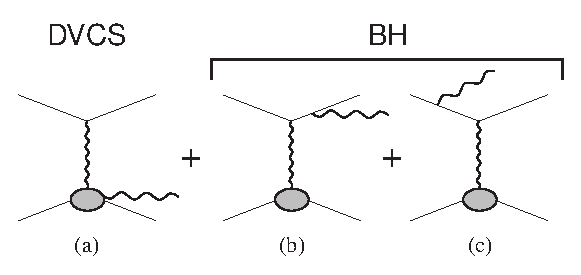
\epsfig{file=../der/diagbh.eps}}
\caption{\small{Diagrams contributing to the electroproduction of a real 
photon. The DVCS process (a) is shown along with the interfering Bethe-Heitler
diagrams (b) and (c).}} 
\label{dvcsbh}
\end{figure}
%%%%%%%%%%%%%%%%%%%%%%%%%%%%%%%%%%%%%%%%%%%%%%%%%%%%%%%%%%%%%%%%%%%%%%%%

The total amplitude $\mathcal T$ is the superposition of the BH and DVCS 
amplitudes:

\begin{eqnarray}
\left | \mathcal T \right |^2 & = & \left | \mathcal T_{BH} \right |^2+\left |
\mathcal T_{DVCS} \right |^2+ \mathcal I \\
\mathcal I & = & \mathcal T_{DVCS}^* \mathcal T_{BH} +
\mathcal T_{DVCS} \mathcal T_{BH}^* \, ,
\end{eqnarray}

\noindent 
where $\mathcal T_{DVCS}$ and $\mathcal T_{BH}$ are the amplitudes for the 
DVCS and Bethe-Heitler processes, and $\mathcal I$ denotes the interference 
between these amplitudes. The individual contributions to the total 
$e p \to e p \gamma$ cross section can be written as (up to twist-3 
contributions)~\cite{Belitsky:2001ns} as:

\begin{eqnarray}
\left| \mathcal T_{BH} \right|^2 & = & \frac{\Gamma_{BH}(x_B,Q^2,t)}{\mathcal P_1(\varphi) P_2(\varphi)}
\left\{ c_0^{BH} + \sum_{n=1}^2 c_n^{BH} \cos (n\varphi) +s_1^{BH} \sin\varphi \right\}  \, , \label{eq:epepgBH} \\
\left| \mathcal T_{DVCS} \right|^2 & = & \Gamma_{DVCS}(x_B,Q^2,t)
\left\{ c_0^{DVCS} + \sum_{n=1}^2 [ c_n^{DVCS} \cos (n\varphi) +s_n^{DVCS} \sin(n\varphi) ] \right\} \, , \label{eq:epepgDVCS} \\
\mathcal I & = & \frac{\Gamma_{I}(x_B,Q^2,t)}{\mathcal P_1(\varphi) P_2(\varphi)} ]
\left\{ c_0^{I} + \sum_{n=1}^3 [ c_n^{I} \cos (n\varphi) +s_n^{I} \sin(n\varphi) ] \right\} \, , \label{eq:epepgI}
\end{eqnarray}

\noindent 
where $\mathcal P_1(\varphi)$ and $\mathcal P_2(\varphi)$ are the BH electron 
propagators and $c_i,s_i$ are azimuthal moments in the corresponding cross 
section contributions.

Depending on whether the beam helicity or target spin is flipped, different 
GPD contributions enter the cross section azimuthal moments ($\sigma_{LU},
\sigma_{UL}$).  In practice, cross section asymmetries are experimentally 
easier to determine:

\begin{equation}
A=\frac{d\sigma^\leftarrow-d\sigma^\rightarrow}{d\sigma^\leftarrow+d\sigma^\rightarrow}\simeq\Gamma_A(x_B,Q^2,t)\frac{s_1^I \sin\varphi + s_2^I \sin 2\varphi}
{c_0^{BH}+c_0^I+\Gamma_Dc_0^{DVCS}+(c_1^{BH}+c_1^I+\Gamma_Dc_0^{DVCS})\cos\varphi} \, ,
\end{equation}

\vskip 0.3cm

\noindent 
where $\Gamma_A,\Gamma_D$ are  known kinematical prefactors. 

DVCS measurements thus allow one to separate the imaginary and real parts of 
the DVCS amplitude (\textit{cf.}\ Fig.~\ref{fig:handbag}) by measuring 
combinations of cross sections and asymmetries with respect to the beam spin 
(helicity), beam charge ($e^+/e^-$), and/or target or recoil polarization. 
The imaginary part of the amplitude probes the GPDs at $x=\xi = \xbj/2$,
the real part probes a certain integral over the quark momentum fractions. 

The different nucleon spin components of the GPDs can be extracted by 
measuring target spin asymmetries. Measurements of the $t$ ($\Delta_\perp$) 
dependence provide the information necessary for transverse nucleon imaging. 
Information about the flavor decomposition requires measurements with both 
protons and neutrons.   Additional information about the spin/flavor 
separation can come from meson production data. Studies of DVCS and meson 
production processes will require a combination of high energy and high beam 
intensity, and are generally much more challenging than traditional inclusive 
scattering experiments.

The {\tt CLAS12} setup will provide unprecedented capabilities for exploring 
nucleon structure in the valence quark region. In particular, it will provide
the  combination of high beam intensity (luminosity), high energy, high beam 
polarization, and advanced detection capabilities to provide a unique 
opportunity for studying nucleon GPDs in exclusive processes in the valence 
region.

\section{Present Experimental Results on Hard Exclusive Processes}

Measurements of exclusive processes at large momentum transfers 
have been carried out in $eN$ scattering experiments with existing 
fixed--target facilities (HERMES at DESY, JLab with 6~GeV beam 
energy) and the HERA collider. These studies have demonstrated the basic 
feasibility of such measurements, and have provided crucial evidence for 
the applicability of a GPD--based description of such processes.
They are also providing the first useful constraints for GPD phenomenology.

Experiments at fixed--target facilities aim to extract the
interference terms between the DVCS and the Bethe--Heitler (BH) amplitudes
in the $eN \to e'N\gamma$ cross section. The interference terms are 
experimentally accessible from combinations of measurements of the
spin--dependent and independent cross sections and relative asymmetries,
as well as from measurements of the beam charge dependence ($e^+ / e^-$)
of the cross section. In kinematic regions where the BH amplitude is much 
larger than the DVCS amplitude, the interference with the BH amplitude acts 
as a natural ``amplifier and filter'' for the DVCS amplitude, boosting
it to comfortably measurable levels. 

%%%%%%%%%%%%%%%%%%%%%%%%%%%%%%%%%%%%%%%%%%%%%%%%%%%%%%%%%%%%%%%%%%%%%%%%
\begin{figure}[ht]
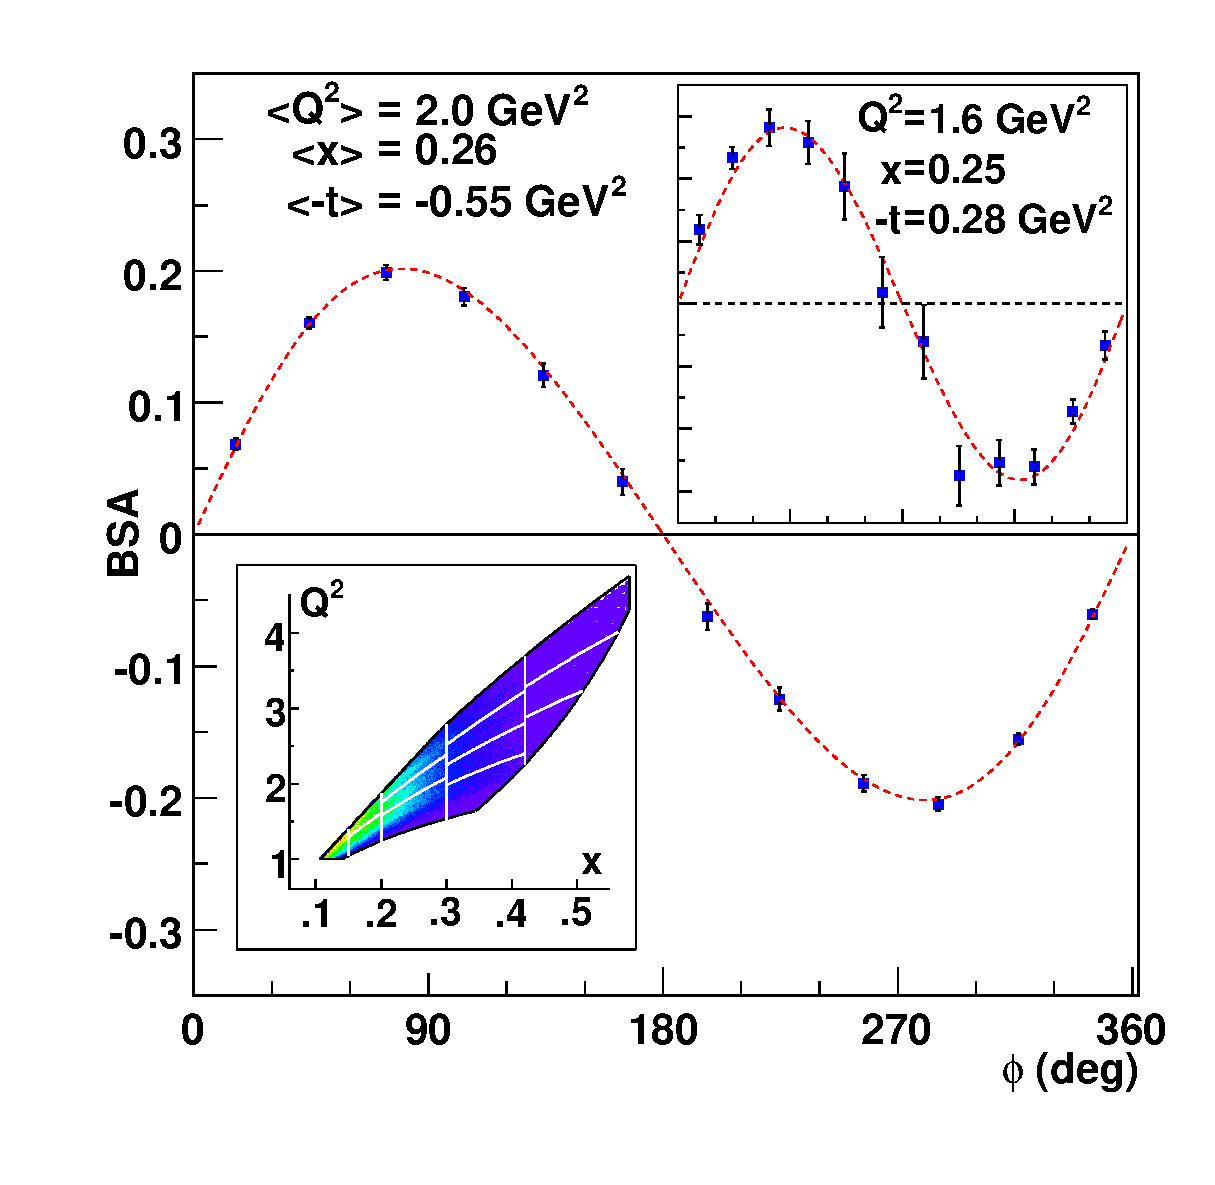
\includegraphics[width=0.99\textwidth]{../der/WP_CLAS_ALU.eps}
\caption{\small{Measurements of the beam spin asymmetry, $A_{LU}$, of the 
$eN \to e'N\gamma$ cross section from {\tt CLAS} at 6~GeV.  The plot in
the lower left corner shows the kinematic coverage in $\xbj$ and $Q^2$.
The main plot shows the beam spin asymmetry vs. $\phi$ integrated over all
kinematics (the average values are shown in the upper left of the plot.  In
the upper right of the plot, the beam spin asymmetry is shown for one of
our many kinematic points as an illustration.  The $\sin \phi$ dependence 
is characteristic of the BH-DVCS interference cross section.  The magnitude 
of the asymmetry can be related to a linear combination of the GPDs 
at $x = \xi$.}}
\label{fig:CLAS_e1}
\end{figure}
%%%%%%%%%%%%%%%%%%%%%%%%%%%%%%%%%%%%%%%%%%%%%%%%%%%%%%%%%%%%%%%%%%%%%%%%

Measurements of the beam spin asymmetry in $eN \to e'N\gamma$ have been 
performed by HERMES ($0.02 < \xbj < 0.3$)~\cite{Airapetian:2001yk}, {\tt CLAS}
\cite{Stepanyan:2001sm,JLabExp:E01-113} and Hall A ($0.15 < \xbj < 0.55$)
\cite{JLabExp:E00-110}.  Fig.~\ref{fig:CLAS_e1} shows the kinematic coverage 
of the {\tt CLAS} detector at 5.7~GeV, as well as the results for the 
asymmetry in a typical $(\xbj, Q^2)$ bin.  A new inner calorimeter was used 
to detect photons at small scattering angles.  The azimuthal angle dependence 
of the asymmetry clearly exhibits the $\sin\phi$ behavior characteristic
of the BH--DVCS interference. This asymmetry can be related to a linear 
combination of GPDs at $x = \xi$; the experimental results are consistent 
with the predictions of present GPD models. An important point is that with 
the {\tt CLAS} detector data in all $(\xbj, Q^2, t)$ bins are taken 
simultaneously, making it possible to extract information about the GPDs 
over a wide kinematic range.

While the unpolarized GPD $\cal H$ dominates the beam spin asymmetry at 
small $t$~\cite{Belitsky:2001ns}, $\sigma_{LU} \sim F_1{\cal H}-\xi F_2{\cal 
\widetilde H}$, the target single spin asymmetry at small $t$ has a 
significant contribution from the polarized GPD $\cal \widetilde H$
\cite{Belitsky:2001ns}: $\sigma_{UL} \sim F_1{\cal \widetilde H}-\xi 
F_2{\cal H}$.  Therefore, a combined analysis of the beam and target single 
spin asymmetries will allow for separation of $\cal H$ and $\cal \widetilde H$.

Recently published results by the {\tt CLAS} collaboration on the first 
measurements of the target spin asymmetry~\cite{Chen:2006na} confirmed again 
that the factorization is likely to be applicable at $Q^2$ values as low as 
2~GeV$^2$. These measurements eventually will allow one to separate the 
contributions from unpolarized and polarized nucleon GPDs.  An order of 
magnitude more data are expected from JLab during the next two years, which 
would allow for more accurate extraction of GPD parameters. 

The measurements of the DVCS cross sections and beam spin asymmetries carried 
out by JLab with 6~GeV beam energy support the theoretical expectation of 
dominance of the single-quark reaction mechanism (leading-twist approximation) 
for DVCS for momentum transfers $Q^2$ of a few GeV$^2$, essential for the GPD 
interpretation of the $eN \to e'N\gamma$ data.  They also demonstrate the 
feasibility of accurate differential measurements of the $t$-dependence of the 
cross sections needed for the GPD-based reconstruction of the spatial images 
of the nucleon.

The HERMES collaboration measured for the first time the beam charge 
asymmetry of the cross section, which probes a dispersive integral of the 
GPDs over the quark momentum fractions \cite{Airapetian:2006zr}.  DVCS 
cross sections at high $Q^2$ were measured at HERA
\cite{Chekanov:2003ya,Adloff:2001cn}, including its $t$-dependence; the 
results are well described by leading-order (LO) and next-to-leading order 
(NLO) QCD calculations incorporating QCD evolution of the GPDs, thus fully 
confirming the applicability of QCD factorization to exclusive processes 
at high energies.

\subsection{GPD Measurements with Jefferson Laboratory at 12 GeV}

{\tt CLAS12} will provide a unique combination of high beam intensity 
(luminosity), high energy, and large--acceptance detectors, which will 
enable studies of exclusive processes such as DVCS and meson production 
in the valence quark region.

%%%%%%%%%%%%%%%%%%%%%%%%%%%%%%%%%%%%%%%%%%%%%%%%%%%%%%%%%%%%%%%%%%%%%%%%
\begin{figure}[ht]
\centerline{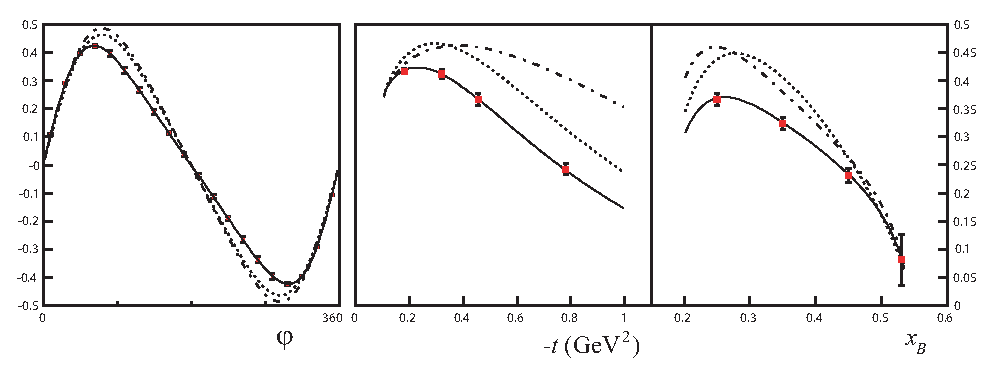
\epsfig{file=../der/asymmetry_detail.eps,width=\linewidth}}
\caption{\small{On all figures: points in red represent data with statistical 
error bars. Lines are models with different input parameters, none of which 
includes twist-3 contributions:  The full line is a model with a Regge-type 
$t$-dependence and D-term. The dotted line includes the Regge-type 
$t$-dependence but has no D-term. The dash-dotted line has the D-term but the 
$t$ dependence only comes from form factors. Left figure: Beam spin asymmetry 
(BSA) as a function of $\varphi$ for $<x_B>=0.2$, $<Q^2>=3.3$~GeV$^2$, and 
$<-t>=0.45$~GeV$^2$. Middle figure: BSA as a function of $-t$ for $<x_B>=0.2$, 
$<Q^2>=3.3$~GeV$^2$, and $\varphi=90^\circ$. Right figure: BSA as a function 
of $x_B$ for $t=0.45$~GeV$^2$, $<Q^2>=3.3$~GeV$^2$ and $\varphi=90^\circ$.}}
\label{fig:asymbig}
\end{figure}
%%%%%%%%%%%%%%%%%%%%%%%%%%%%%%%%%%%%%%%%%%%%%%%%%%%%%%%%%%%%%%%%%%%%%%%%

Detection of the photon in the {\tt CLAS} inner calorimeter, in addition 
to the recoil proton and scattered electron, provides the exclusivity 
condition crucial for complete control over different background processes. 
Using the $epX$ sample  has its own advantages with regard to background 
suppression ($\pi^0$) and azimuthal angle coverage.  The two samples probe 
$ep \to e'\gamma p$ in regions of different relative magnitudes of the DVCS 
and Bethe-Heitler amplitudes.  In this way, GPDs can be extracted using both 
absolute cross section and polarization asymmetry data. The possibility to 
use both methods in experiments at a single facility represents a crucial 
advantage of {\tt CLAS12}.

%%%%%%%%%%%%%%%%%%%%%%%%%%%%%%%%%%%%%%%%%%%%%%%%%%%%%%%%%%%%%%%%%%%%%%%%
\begin{figure}[ht]
\begin{center}
\epsfig{file=../der/tsa_phi_comp.epsi, totalheight=15cm, width=6.5cm, angle=270}
\caption{\small{(a). Target spin asymmetry versus $\varphi$ for 
$Q^2$=4.1~GeV$^2$, $x_B$=0.36, and $-t$=0.52~GeV$^2$. The black points show 
the values from Ref.~\cite{Vanderhaeghen:1999xj} using CTEQ6 PDFs with the 
estimated errors from the proposed measurement. The red solid curve is using 
MRST02 PDFs with $E=\widetilde{E}$=0, and for the blue dashed curve is 
$\widetilde{H}$ is also set to zero. (b). $\sin{\varphi}$ moments of the 
target spin asymmetry versus $-t$ at $Q^2$=4.1~GeV$^2$ and $x_B$=0.36, and 
(c). versus $x_B$ at $Q^2$=4.1~GeV$^2$ and $-t$=0.52~GeV$^2$. The projected 
error bars represent the statistical uncertainties only.}} 
\label{Fig:TsaPhiComp}
\end{center}
\end{figure}
%%%%%%%%%%%%%%%%%%%%%%%%%%%%%%%%%%%%%%%%%%%%%%%%%%%%%%%%%%%%%%%%%%%%%%%%

To separate the different spin components of the GPDs, measurements of a 
variety of polarization observables (beam and target spin) will be performed. 
The longitudinal beam single spin asymmetry, $A_{LU}$ (see 
Fig.~\ref{fig:asymbig}), will access mainly the unpolarized Dirac GPD, 
$\cal H$.  Combined analysis of the DVCS data on a longitudinally polarized 
target single spin asymmetry (see Fig.~\ref{Fig:TsaPhiComp}) with the beam 
single spin asymmetry will provide separation of contributions from 
unpolarized and polarized GPDs.  The double spin asymmetry for longitudinal 
target polarization, $A_{LL}$, provides information on the real part of the 
corresponding GPDs, complementary to beam charge asymmetries.
 
The results of these measurements can directly be translated into transverse 
spatial images of the nucleon. As an example, Fig.~\ref{fig:H_proj} shows 
the projected results for the Dirac GPD, $\cal H$, as a function of $x$ and 
$t$, and its corresponding transverse spatial representation.  Complementary 
information can be obtained about integrals of the GPDs over the quark 
momentum fraction. With the help of GPD parameterizations, this information 
can be used to construct 2-dimensional tomographic images of the nucleon.

%%%%%%%%%%%%%%%%%%%%%%%%%%%%%%%%%%%%%%%%%%%%%%%%%%%%%%%%%%%%%%%%%%%%%%%%
\begin{figure}
\begin{tabular}{cc}
\parbox[c]{0.4\textwidth}{
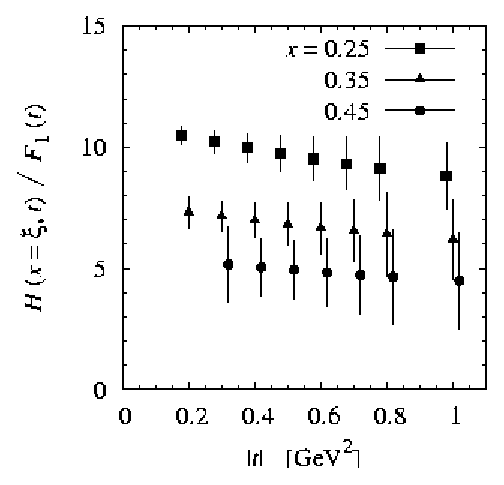
\includegraphics[width=0.4\textwidth]{../der/gpdtdep.eps}}
&
\parbox[c]{0.56\textwidth}{
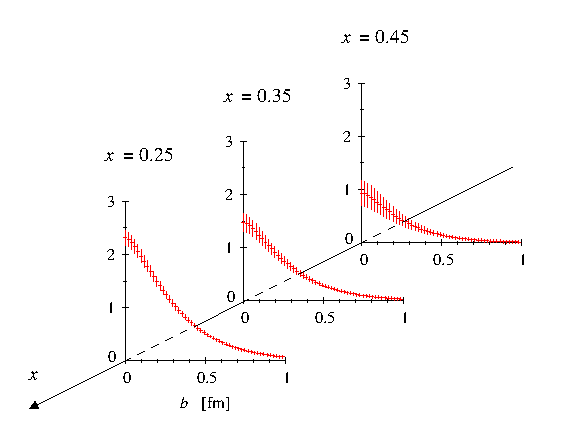
\includegraphics[width=0.56\textwidth]{../der/spatial_narrow.eps}}
\end{tabular}
\caption{\small{Left: Projected results for the Dirac GPD of the proton, 
${\cal H}(x = \xi, t)$, as a function of $x$ and $t$, as extracted from the 
DVCS beam spin asymmetry, $A_{LU}$, measured at JLab at 12~GeV. Shown is the 
ratio of the GPD to the the proton's Dirac form, $F_1(t)$.  Right: Transverse 
spatial image of the proton obtained by Fourier-transforming the measured GPD. 
The errors were estimated assuming a dipole-like $t$-dependence.}}
\label{fig:H_proj}
\end{figure}
%%%%%%%%%%%%%%%%%%%%%%%%%%%%%%%%%%%%%%%%%%%%%%%%%%%%%%%%%%%%%%%%%%%%%%%%

Additional information about the flavor structure of GPDs will come from 
ratios of meson production cross sections in channels with the same 
spin/parity quantum numbers, such as $\eta / \pi^0$ and $K^* / \rho^+$. 
These channels will be measured simultaneously with DVCS, not requiring any 
extra beam time.

Measurements of exclusive meson production in non-diffractive channels in
{\tt CLAS12} would allow for detailed studies of the spin, flavor, and 
spatial distributions of quarks in the nucleon in the valence region, 
complementing the information from DVCS measurements.  Very interesting 
information can already be gained by comparing observables for different 
mesonic channels, without detailed modeling of the GPDs.  For example, a 
comparison of $\pi^0$ and $\eta$ provides model-independent information 
about the ratio of the quark spin distributions $\Delta u$ and $\Delta d$ 
and their spatial distributions.  Comparison between $\pi^+$ and $K^+$ 
production, as well as between $\rho^+$ and $K^{*+}$, allows one to study 
$SU(3)$ flavor symmetry breaking in the nucleon's quark distributions in 
different spin/parity channels.  More information about the spatial 
distribution of quarks can be obtained from the GPD analysis of absolute 
cross sections ($\sigma_L$) in these channels.  Separation of the various 
response functions ($L$, $T$, etc.) would provide a crucial test of the 
dominance of the single-quark reaction mechanism at large $Q^2$.

Another interesting class of processes that could be studied are exclusive 
reactions with $N \to N^*$ transitions.  Such processes probe the 
``transition GPDs'' -- the probability amplitude for the nucleon to  
undergo a transition to an excited state when ``taking out'' a quark and 
``putting it back'' with different momentum. In these reactions the hard 
scattering process can be regarded as an operator inducing an $N \to N^*$ 
transition. {\tt CLAS12} is capable of performing such measurements requiring 
detection of decay products of the recoiling nucleon resonances.

\section{GPD Studies with a Transversely Polarized Target}

Asymmetries in the exclusive production of photons and vector mesons with a
transversely polarized target were identified as the most sensitive 
observables providing access to the total orbital angular momentum.  Eight 
observables, namely the first harmonics $\cos \phi$ and $\sin \phi$ of the 
interference term, are accessible in polarized beam and target experiments 
\cite{Belitsky:2001ns}.  Thus, experiments with both longitudinally and
transversely polarized targets can measure all eight Fourier coefficients
$c_{1,{\mit\Lambda}}^{\cal I}$ and $s_{1,{\mit\Lambda}}^{\cal I}$ and
with ${\mit\Lambda} = \{ {\rm unp}, {\rm LP}, {\rm TP}_x, {\rm TP}_y \}$. 

The DVCS single spin asymmetry (SSA) for a transversely polarized target is 
the most sensitive observable to the elusive GPD $\cal E$, providing access 
to the orbital angular momentum.  First results on DVCS single spin asymmetries 
from the HERMES Collaboration for transverse target polarizations~\cite{HERAUT} 
indeed indicate great sensitivity of target single spin asymmetries to the 
contribution of $u$-quarks to the total angular momentum.  The most 
sensitive to the GPD-$\cal{E}$ asymmetry appeared to be the $\cos \phi$ moment 
of the spin-dependent contribution $\sigma_{UT}$~\cite{Belitsky:2001ns},

\begin{equation}
\label{AUT}
\sigma_{UT} \sim \frac{1-x}{2-x}\frac{t}{M^2}F_2{\cal H}
+ \frac{t}{4M^2}(2-x)F_1{\cal E}.
\end{equation}

Transverse target DVCS SSA measurements in addition to unpolarized SSA and 
longitudinally polarized SSA measurements will provide the full set of data 
needed for the extraction of Compton form factors and corresponding GPDs. 
$A_{UT}$ is especially sensitive to the GPD $\cal E$, and as such will
constrain any extraction of the angular momentum $J$.

The projection curves for {\tt CLAS12} running with a transversely polarized 
target have been calculated assuming a luminosity of 
$5 \times 10^{34}$~cm$^{-2}$s$^{-1}$, with an $NH_3$ target polarization of 
85\% and a dilution factor 0.14, with 2000 hours of data taking and an 
overall efficiency 50\% (see Fig.~\ref{fig:autdvcs}).

%%%%%%%%%%%%%%%%%%%%%%%%%%%%%%%%%%%%%%%%%%%%%%%%%%%%%%%%%%%%%%%%%%%%%%%%%%%%
\begin{figure}[htbp]
\vspace{7.0cm}
\special{psfile=../der/autproj11.eps hscale=45 vscale=55 hoffset=-30 voffset=-10}
\special{psfile=../der/rhoasym_cdr.eps hscale=45 vscale=40 hoffset=210 voffset=-10}
\caption{\small Projected transverse spin asymmetry ($A_{UT}^{\sin\phi}$)
in exclusive photon production at 11~GeV.  All points correspond to different 
values of $J_u$ calculated for the bin with $<Q^2>$=2.6~GeV$^2$ and 
$<x>=0.25$ (left). Projections for the transverse target asymmetry for exclusive
$\rho^0$ production from a hydrogen target (filled squares) using {\tt CLAS12} 
are shown compared to preliminary HERMES data~\protect\cite{hermesrho}.}
\label{fig:autdvcs}
\end{figure}
%%%%%%%%%%%%%%%%%%%%%%%%%%%%%%%%%%%%%%%%%%%%%%%%%%%%%%%%%%%%%%%%%%%%%%%%%%%%

The theoretical uncertainty in the factorization procedure on the amplitude 
level for the meson sector is translated into large variations of the physical 
cross section.  However, in the single-spin asymmetry, given by the ratio
of the Fourier coefficients of the cross section, the ambiguities 
approximately cancel~\cite{Belitsky:2003tm}.  Thus, the perturbative 
predictions for this quantity are rather stable. The NLO effects result in 
${}^{+ 7 \%}_{- 18 \%}$ corrections to the LO prediction for 
$0.1 < \xbj < 0.5$.

The GPD-based calculations were performed for the case when the incoming 
virtual photon is longitudinally polarized.  The cross section for the 
transversely polarized photons is suppressed by a power of $Q$
\cite{Collins:1996fb}, but at {\tt CLAS} energies it may still be significant. 
Insensitivity to the higher-order corrections make single spin asymmetries
appropriate quantities for experimental study at JLab, and will provide an 
important test of the applicability of GPD-based predictions at JLab energies.

Even though the power corrections for the absolute cross section of exclusive
meson electroproduction analyzed in terms of generalized parton distributions
are expected to be large, there are indications of a {\it precocious scaling} 
in the ratios of observables~\cite{Belitsky:2003tm}.  The measurement of spin 
asymmetries could therefore become a major tool for studying GPDs in the 
$Q^2$ domain of a few GeV$^2$. Projections for {\tt CLAS12} for measurements 
of transverse asymmetries for vector mesons are shown in 
Fig.~\ref{fig:autdvcs}.  The transverse asymmetries for $\rho$ mesons (neutral 
and charged) are widely accepted as an important source of independent 
information on the GPD $\cal{E}$.  SSA measurements in hard exclusive processes 
will allow mapping of the underlying GPDs and will provide access to the 
orbital angular momentum of quarks.

The quark angular momentum in the nucleon, $J_q$, can be estimated if one 
uses the results of measurements of DVCS and meson production observables to 
constrain GPD parameterizations, which incorporate information about GPDs 
obtained from other processes (inclusive DIS, form factors). These 
parameterizations allow one to estimate the second moment of the GPDs, based 
on the information about the GPDs at $x_1 = x_2$ and the momentum fraction 
integrals probed in the observables. Fig~\ref{fig:autdvcs} shows the
constraints on $J_u$ and $J_d$ from DVCS and $\rho$ asymmetries, which is 
particularly sensitive to the Pauli form factor-type GPD, $\cal E$.  One sees 
that accurate measurements of the asymmetries will be able to constrain $J_q$ 
in this way. While not fully model--independent, this method of extracting 
$J_q$ will become more and more accurate as amplitude calculations and GPD 
parameterizations become more refined as a result of measurements of a 
variety of other DVCS and meson production observables.  High statistics data 
will allow us to constrain the quark angular momentum in the proton.

The data from {\tt CLAS} with a transversely polarized target focussing
on hard exclusive photon and meson production, combined with data from 
unpolarized and longitudinally polarized targets, will provide a complete set 
of measurements required for the separation of all four leading-twist,
chiral-even GPDs, and in particular, will provide a constraint on the quark 
orbital angular momentum.


\section{Summary}

GPDs unify the momentum-space parton densities measured in inclusive 
deep-inelastic $eN$ scattering with the spatial densities (form factors) 
measured in elastic scattering.  They describe correlations between the 
momentum and spatial distributions of quarks, which are revealed in 
exclusive processes in $eN$ scattering at large momentum transfer (deeply 
virtual Compton scattering, meson production).

A full program to extract GPDs from measurements requires coverage of a 
large kinematic range in $\xi$, $t$, and $Q^2$, along with measurements of 
several final states together with the use of polarized beam and polarized 
targets (both longitudinal and transverse polarization).  The 12-GeV upgrade 
of the electron accelerator and of the equipment required for the GPD program 
will provide the kinematic coverage needed for a broad program of DVCS and 
meson production measurements.  The JLab 12-GeV upgrade will allow us to map 
the nucleon GPDs in the valence quark region at large $x$, exploring its quark 
structure in unprecedented detail.

%
\chapter{Parton Distributions at Large $x$}

\section{Parton Distributions} 
\label{F2A1}

Knowledge of parton distributions forms the basis of our understanding
of hadronic matter in terms of its fundamental constituents.  However, 
extracting parton distributions in the large $x$ domain is notoriously 
difficult.  One difficulty comes from the requirement to stay away from
the region where partonic initial and final state interactions play 
important roles.  This imposes a minimum $Q^2$ threshold of at least a few 
GeV$^2$ and $W$ greater than a few GeV in addition to the large $x$ constraint.
For polarized parton distributions, an additional problem stems from the lower 
luminosity available with polarized targets.  In the unpolarized case, 
luminosities are adequate and free proton targets exist, so proton data are 
satisfactory.  For the neutron no such targets exist and deuteron is used. 
The difficulty is to control sufficiently well nuclear final state 
interactions (FSI) and binding effects to allow for a systematically accurate 
extraction of the neutron information. 

%%%%%%%%%%%%%%%%%%%%%%%%%%%%%%%%%%%%%%%%%%%%%%%%%%%%%%%%%%%%%%%%%%%%%%%%%%%
\begin{figure}[htbp]
\vspace{6.5cm}
\special{psfile=../strucfunc/largex.eps hscale=75 vscale=75 hoffset=10 voffset=-205}
\caption{\small{World data on the $d/u$ parton distribution ratio from 
unpolarized measurements of $F_2^n/F_2^p$ (left) and on the photon asymmetry 
$A_1^n$ from polarized data (right).  The substantial systematic (left) or 
statistical (right) errors at large $x$ do not permit constraints of the 
various predictions.}}
\label{fig:largex} 
\end{figure}
%%%%%%%%%%%%%%%%%%%%%%%%%%%%%%%%%%%%%%%%%%%%%%%%%%%%%%%%%%%%%%%%%%%%%%%%%%%

The consequences of these difficulties can be readily seen in 
Fig.~\ref{fig:largex}.  The lack of experimental constraints allows for a 
variety of predictions that needs to be sorted out to establish the proper
phenomenology. Studies of parton distributions have already been undertaken 
at JLab, with $x \leq 0.6$. The BONUS experiment~\cite{BONUS} gathered 
neutron data from quasi-free neutrons within unpolarized deuterons.  The 
FSI and binding effects were minimized by measuring recoiling protons and 
selecting events for which the two nucleons were not interacting.  On the 
polarized data front, data were collected up to $x \sim 0.6$ in Halls A and 
B~\cite{Zheng:2004ce, Dharmawardane:2006zd}.  An exciting outcome is the 
apparent failure of leading order (LO) pQCD to describe the data, hinting 
that the validity domain of LO pQCD is not reached yet or that quark orbital 
momentum (an important but experimentally elusive contribution to the nucleon 
spin) may be sizable. In particular, LO pQCD predicts that the $d$-quark 
polarization (lower panel Fig.~\ref{fig:E99117}) should become positive and 
approach +1 at large $x$, which is in contradiction to the data.

%%%%%%%%%%%%%%%%%%%%%%%%%%%%%%%%%%%%%%%%%%%%%%%%%%%%%%%%%%%%%%%%%%%%%%%%%%% 
\begin{figure}
\vspace{9.0cm}
\special{psfile=../strucfunc/delq_new1.eps hscale=70 vscale=60 hoffset=80 voffset=-15}
\caption{\small{Quark polarizations $( \Delta u+ \Delta\bar{u})/(u+\bar{u})$ 
and $( \Delta d+ \Delta\bar{d})/(d+\bar{d})$ as extracted from $A_1^n$, 
$A_1^p$, and $A_1^d$~\cite{Zheng:2004ce, Dharmawardane:2006zd}.  Several NLO 
fits to previous measurements are shown, while the leading-order pQCD 
predictions require both polarizations to tend to +1 as $x \to 1$.}}
\label{fig:E99117}
\end{figure}
%%%%%%%%%%%%%%%%%%%%%%%%%%%%%%%%%%%%%%%%%%%%%%%%%%%%%%%%%%%%%%%%%%%%%%%%%%% 

An 11-GeV beam will allow us to reach $x \sim 0.8$. The luminosity expected 
with an unpolarized deuterium gas target needed for the recoil proton tagging 
method is $2 \times 10^{34}$~cm$^{-2}$s$^{-1}$.  It will be about 
$10^{35}$~cm$^{-2}$s$^{-1}$ for the polarized target currently under design. 
Those luminosities and the large solid angle of {\tt CLAS12} makes it a 
superior choice to measure parton distributions at large $x$, sort out 
mechanisms of SU(6) symmetry breaking and of quark-hadron duality, and explore 
the role of quark orbital momentum.  In addition to their intrinsic interest, 
quark distributions at large $x$ are crucial for studying physics beyond the 
Standard Model at high energy colliders~\cite{Kuhlmann:1999sf}.

To extend the BONUS results to higher $x$, a proposal~\cite{BONUS12} for 
35~days of running on gaseous deuterium and 5~days on gaseous hydrogen at 
11~GeV was submitted to JLab PAC30 and conditionally approved.  The experiment 
will use the standard {\tt CLAS12} equipment with the additional recoil 
detector already used in E03-012~\cite{BONUS}.  The anticipated results can be 
seen in Fig.~\ref{fig:b12xpctd} for $F_2^n/F_2^p$ (left) and $u/d$ (right). 
Clearly the $F_2^n/F_2^p$ data obtained using the new method will allow us to 
differentiate unambiguously between different expectations for this ratio.

%%%%%%%%%%%%%%%%%%%%%%%%%%%%%%%%%%%%%%%%%%%%%%%%%%%%%%%%%%%%%%%%%%%%%%%%%%%
\begin{figure}[ht!]
\begin{center}
\centerline{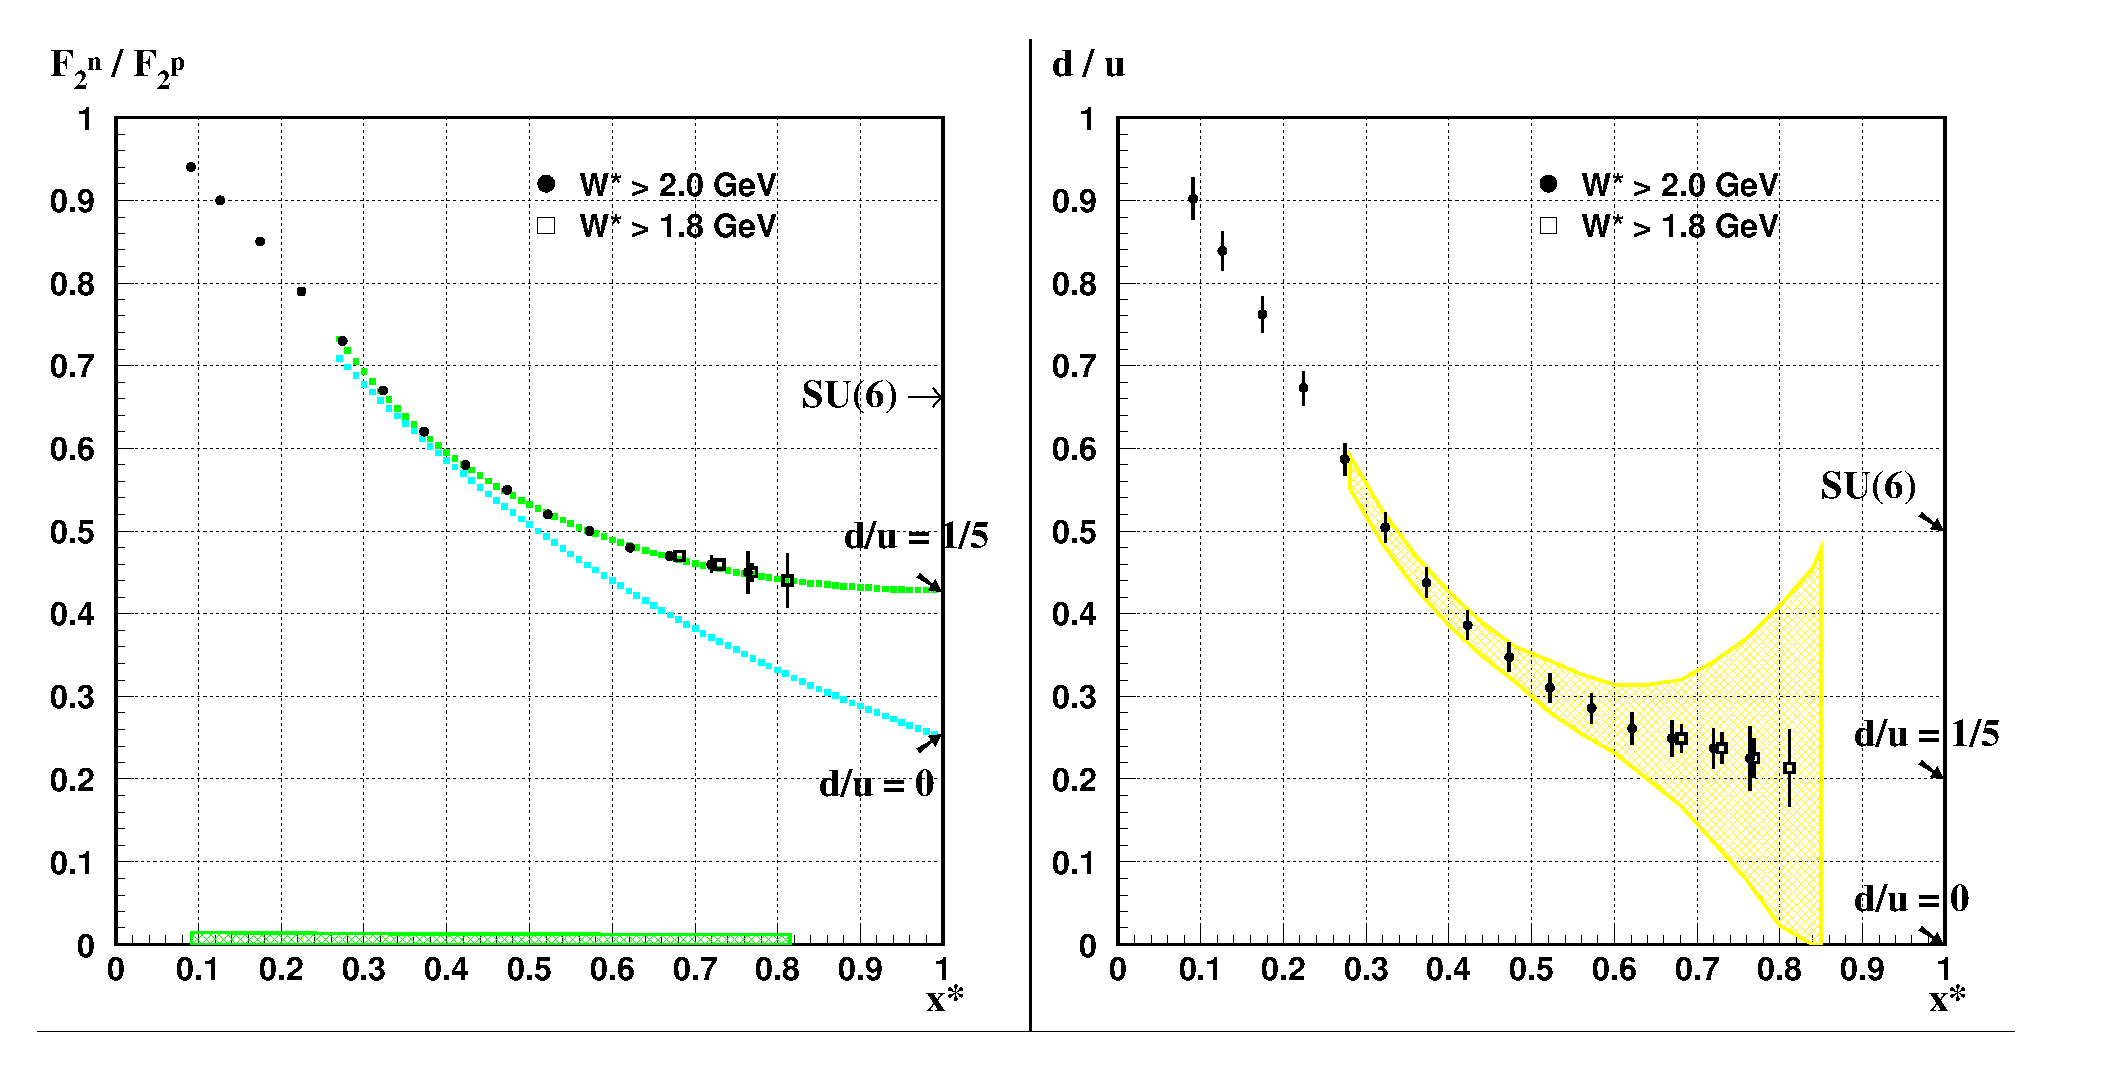
\includegraphics[scale=0.4, angle=0]{../strucfunc/bonus_12_xpctd.eps}}
\end{center}
\vspace*{-1cm}
\caption{\small{Anticipated results on $F_2^n/F_2^p$ (left) and the extracted 
$u/d$ ratio (right) for 40~days of data taking at 11~GeV with {\tt CLAS12}.  
The arrows along the ordinate indicate model predictions.  The error bars 
pertaining to filled circles are statistical with a $W>2$~GeV constraint.  
The smaller errors (with open squares) are for $W>1.8$~GeV.  The systematic 
error is indicated by the band along the abscissa on the left plot.  The two 
curves on the left plot represent hadron-parton duality based predictions 
with two different mechanisms for SU(6) symmetry breaking. The shaded band 
on the right plot indicates our present knowledge on the $d/u$ ratio.}}
\label{fig:b12xpctd}
\end{figure}
%%%%%%%%%%%%%%%%%%%%%%%%%%%%%%%%%%%%%%%%%%%%%%%%%%%%%%%%%%%%%%%%%%%%%%%%%%%

JLab PAC30 also approved E12-06-109 \cite{EG12} which will, in particular,
study polarized parton distributions at large $x$. Using standard detection 
equipment, a redesigned polarized target adapted to {\tt CLAS12} and 30 
(50)~days of running on a longitudinally polarized NH$_3$ (ND$_3$) target, 
high precision measurements can be achieved as shown in Fig.~\ref{fig:A1xpctd}. 
These data will disentangle models in the large-$x$ region.  While the results 
shown in Fig.~\ref{fig:A1xpctd} are with a $W>2$~GeV constraint, hadron-parton 
duality studies (see page \pageref{duality}) will tell us by how much this 
constraint can be relaxed, possibly increasing the $x$ range up to 0.9.  The 
expected accuracy for $(\Delta d+ \Delta\bar{d})/(d+\bar{d})$ is 
shown in Fig.~\ref{fig:ddodxpctd}.
 
%%%%%%%%%%%%%%%%%%%%%%%%%%%%%%%%%%%%%%%%%%%%%%%%%%%%%%%%%%%%%%%%%%%%%%%%%%%
\begin{figure}[ht!]
\begin{center}
\centerline{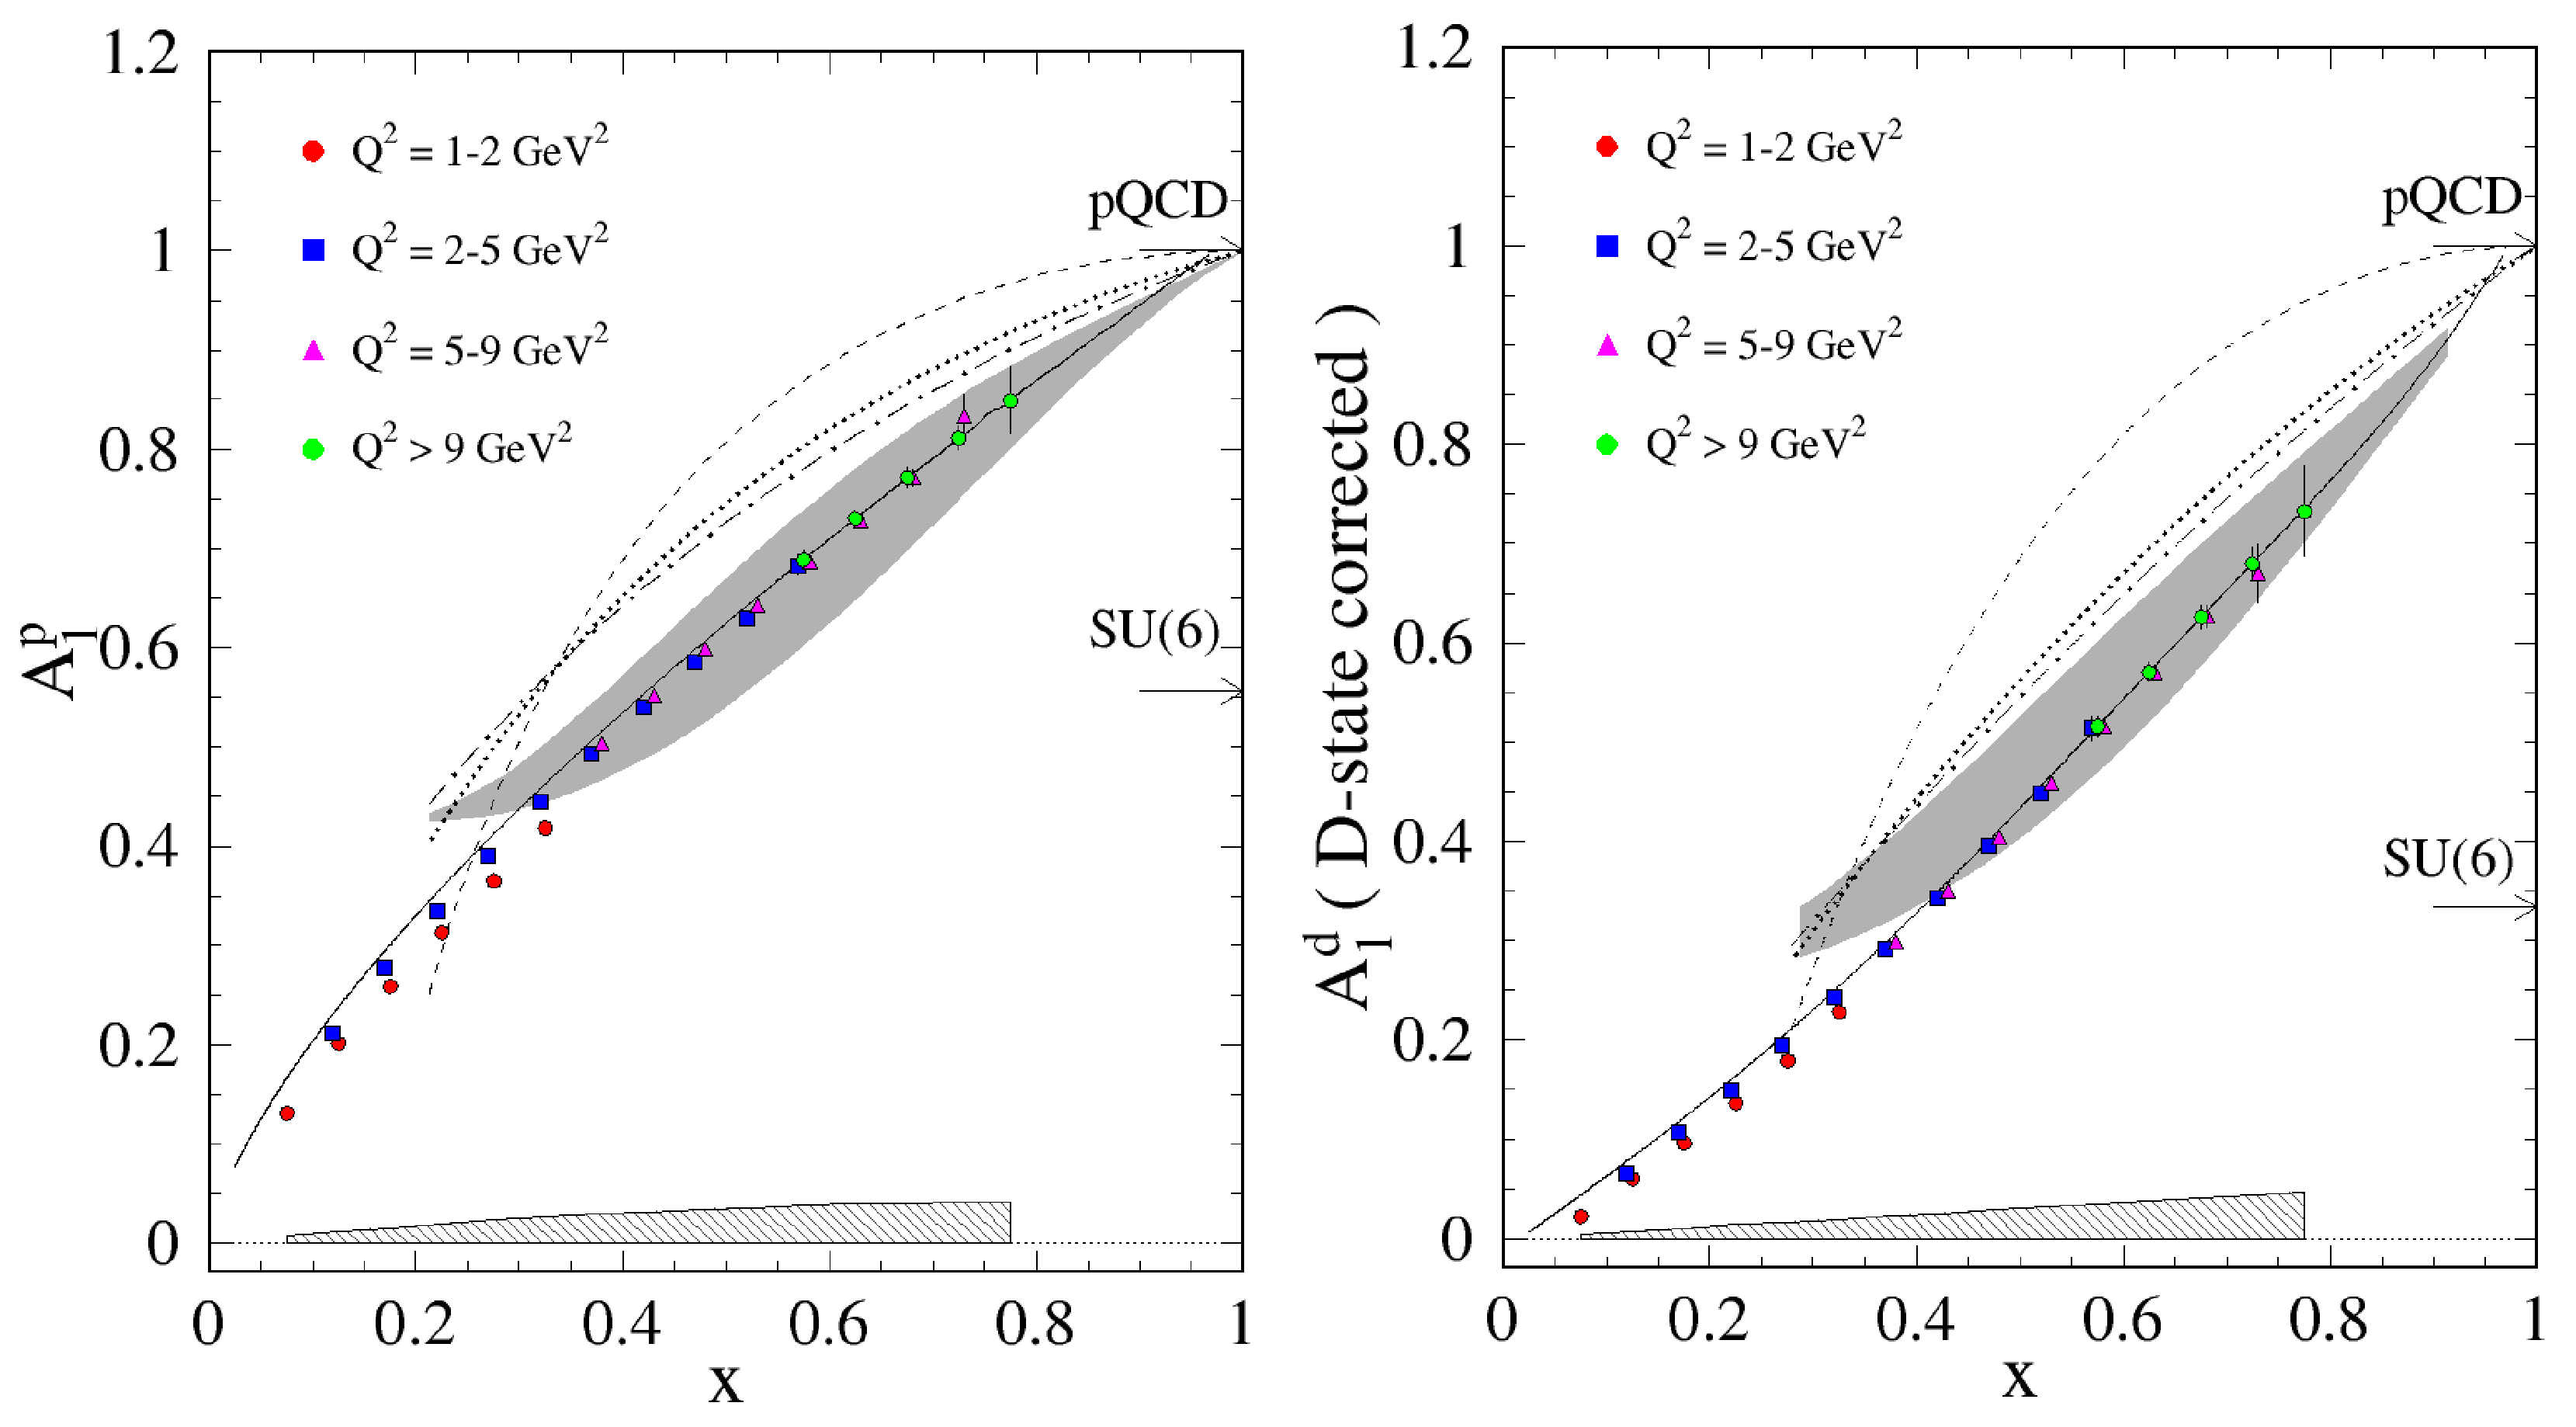
\includegraphics[scale=0.25, angle=0]{../strucfunc/A1_xpctd.eps}}
\end{center}
\vspace*{-1cm}
\caption{\small{Anticipated results on $A_1^p$ (left) and $A_1^d$ (right).
The four different symbols represent four different $Q^2$ ranges.  The 
statistical uncertainty is given by the error bars while the systematic 
uncertainty is given by the shaded band.}}
\label{fig:A1xpctd}
\end{figure}
%%%%%%%%%%%%%%%%%%%%%%%%%%%%%%%%%%%%%%%%%%%%%%%%%%%%%%%%%%%%%%%%%%%%%%%%%%%

%%%%%%%%%%%%%%%%%%%%%%%%%%%%%%%%%%%%%%%%%%%%%%%%%%%%%%%%%%%%%%%%%%%%%%%%%%%
\begin{figure}
\begin{center}
\begin{minipage}[t]{0.55\linewidth}
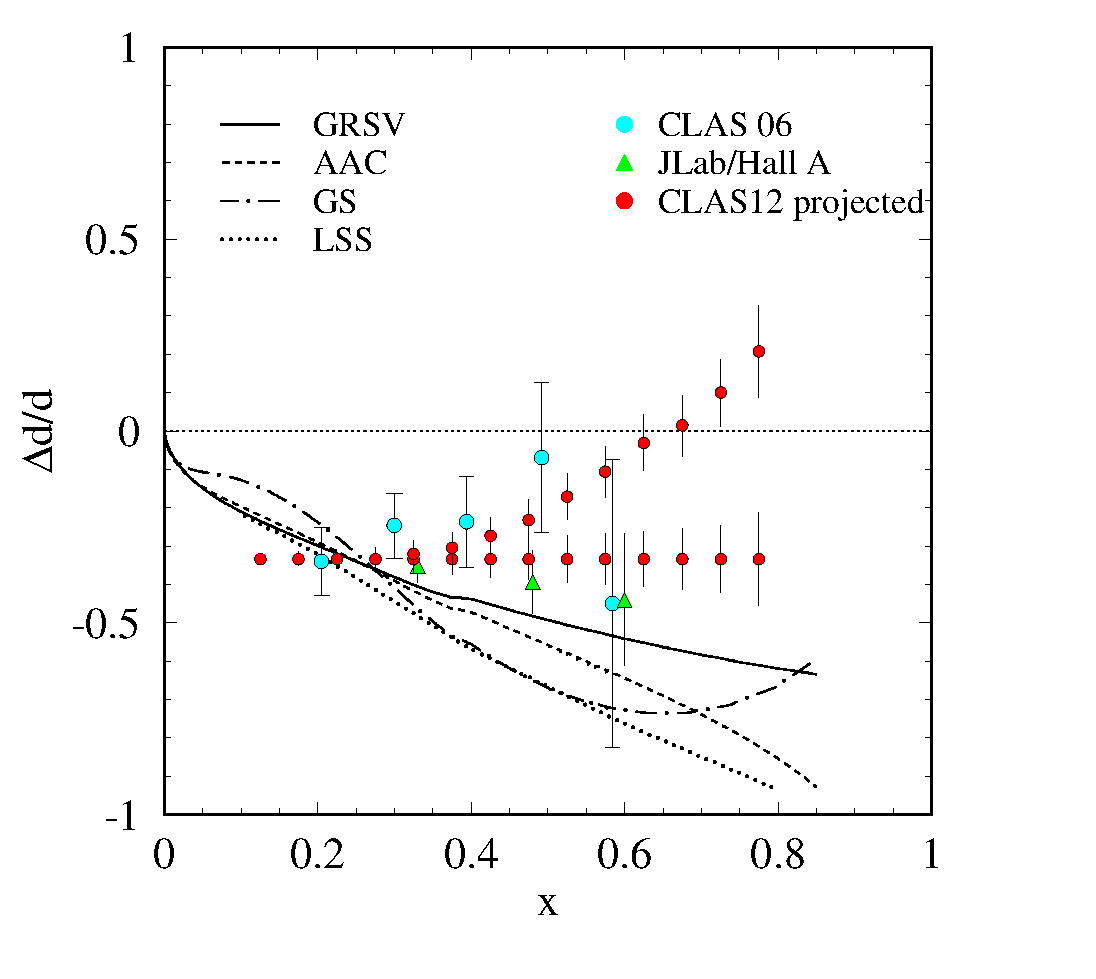
\includegraphics[scale=0.5, angle=0]{../strucfunc/ddod_xpctd.eps}
\end{minipage}\hfill
\begin{minipage}[c]{0.45\linewidth}
\vspace*{-9cm}
\caption{\small{Expected results for $(\Delta d+ \Delta\bar{d})/(d+\bar{d})$. 
The central values of the data are following two arbitrary curves to 
demonstrate how the two categories of predictions, namely the ones that 
predict $\Delta d/d$ stays negative (LO and NLO analyses of polarized 
DIS data: GRSV, LSS, AAC, GS, statistical model, and a quark-hadron duality 
scenario) and the ones predicting $\Delta d/d \to 1$ when $x \to 1$ (leading 
order pQCD and a quark-hadron duality scenario).}}
\label{fig:ddodxpctd}
\end{minipage}
\end{center}
\end{figure}
%%%%%%%%%%%%%%%%%%%%%%%%%%%%%%%%%%%%%%%%%%%%%%%%%%%%%%%%%%%%%%%%%%%%%%%%%%%


\section{Global Fit of Polarized Parton Distributions}

The large window opened by the 12-GeV upgrade over the DIS domain will permit 
constraints of global fits of the parton distributions.  The unique impact at 
large $x$ has just been discussed.  The improvement from the 12-GeV upgrade is 
also significant at low and moderate $x$, noticeably for the polarized gluon 
distribution $\Delta G$.  For a more complete picture of the precision 
achievable with the expected {\tt CLAS12} data, we have plotted in 
Fig.~\ref{pPDFs_exp} an analysis of the impact on NLO analyses.  A dramatic 
improvement can be achieved with the expected data from the {\tt CLAS12} 
proposal E12-06-109~\cite{EG12}.  We emphasize that the data will not only 
reduce the error band on $\Delta G$, but will likely allow a more detailed 
modeling of its $x$-dependence.

%%%%%%%%%%%%%%%%%%%%%%%%%%%%%%%%%%%%%%%%%%%%%%%%%%%%%%%%%%%%%%%%%%%%%%%%%%%
\begin{figure}[htbp]
\vspace{8.5cm}
\special{psfile=../strucfunc/Delu_LSS.eps hscale=55 vscale=55 hoffset=45 voffset=150}
\special{psfile=../strucfunc/Deld_LSS.eps hscale=55 vscale=55 hoffset=245 voffset=150}
\special{psfile=../strucfunc/Delg_LSS.eps hscale=55 vscale=55 hoffset=45 voffset=0}
\special{psfile=../strucfunc/Dels_LSS.eps hscale=55 vscale=55 hoffset=245 voffset=0}
\caption{\small{Expected uncertainties for $\Delta u$, $\Delta d$, $\Delta G$,
and $\Delta s$ from an NLO analysis of all world data.  The outermost line 
shows the result from the analysis by Leader, Sidorov, and Stamenov
\protect{\cite{Leader:2005ci}}.  The second line is the updated result after 
inclusion of the new EG1b data from {\tt CLAS} at 5.7~GeV
\protect{\cite{Dharmawardane:2006zd}}.  The innermost line shows the expected 
uncertainty after including the data set to be collected with {\tt CLAS12}, 
including statistical and systematic errors.}}
\label{pPDFs_exp}
\end{figure}
%%%%%%%%%%%%%%%%%%%%%%%%%%%%%%%%%%%%%%%%%%%%%%%%%%%%%%%%%%%%%%%%%%%%%%%%%%%

 
\section{Moments of Structure Functions}

Moments of structure functions provide powerful insight into nucleon 
structure.  Inclusive data at JLab have permitted evaluation of the moments 
at low and intermediate $Q^2$~\cite{Fatemi:2003yh,Yun:2002td,Chen:2005td}.  
With a maximum beam energy of 6~GeV, however, the measured strength of the 
moments becomes rather limited for $Q^2$ greater than a few GeV$^2$. The 
12-GeV upgrade removes this problem and allows for measurements to higher 
$Q^2$. 

Moments of structure functions can be related to the nucleon static properties 
by sum rules. At large $Q^2$ the Bjorken sum rule relates $\int g_1^{p-n} dx$ 
to the nucleon axial charge~\cite{Bjorken:1966jh}.  At the other end of the 
spectrum, $Q^2$ = 0, the Gerasimov-Drell-Hearn (GDH) sum rule links the 
difference of spin dependent cross sections, integrated over photon energy, 
to the anomalous magnetic moment of the nucleon~\cite{Drell:1966jv,
Gerasimov:1965et}.  The two sum rules are aspects of a general one derived 
recently by Ji and Osborne~\cite{Ji:1999mr} that is valid at any $Q^2$
and links the first moments of spin structure functions to spin-dependent 
Compton amplitudes. Low $Q^2$ is a testing ground for chiral perturbation 
theory, while large $Q^2$ data can be compared to higher-twist series derived 
within the operator product expansion (OPE) method.  Lattice QCD can calculate 
higher-twist terms, thus extending the validity domain of OPE to lower $Q^2$. 
However OPE is unusable at low $Q^2$.  To bridge the gap, lattice QCD can be 
used to compute Compton amplitudes at any $Q^2$.  Hence, the Ji and Osborne 
sum rule can be computed and compared to experiments at any $Q^2$, making it a 
unique tool to study the transition from partonic to hadronic degrees of 
freedom.

%%%%%%%%%%%%%%%%%%%%%%%%%%%%%%%%%%%%%%%%%%%%%%%%%%%%%%%%%%%%%%%%%%%%%%%%%%
\begin{figure}[htb]
\centerline{\epsfxsize=5in\epsfbox{../strucfunc/expect.eps}}
\caption{\small{Left plot: expected precision on $\Gamma_1^p$ for {\tt CLAS12}
and 30~days of running.  {\tt CLAS} EG1a~\cite{Fatemi:2003yh, Yun:2002td} data 
and preliminary results from EG1b are shown for comparison.  The data and 
systematic uncertainties do not include estimates of the unmeasured DIS 
contribution.  HERMES~\cite{Airapetian:2002wd} data, and E143~\cite{Abe:1998wq} 
and E155 data~\cite{Anthony:2000fn} from SLAC are also shown (including DIS 
contribution estimates).  The model is from Burkert and Ioffe
\cite{Burkert:1992tg,Burkert:1993ya}.  Right plot: same as the left but 
including an estimate of the DIS contribution.}}
\label{expect}
\end{figure}
%%%%%%%%%%%%%%%%%%%%%%%%%%%%%%%%%%%%%%%%%%%%%%%%%%%%%%%%%%%%%%%%%%%%%%%%%%

The left plot in Fig.~\ref{expect} shows the expected precision on the 
measured part of $\Gamma_1^p$.  The inner error bar is statistical while the 
outer one is the statistics and systematics added in quadrature.  Published 
results and preliminary results from EG1b are also displayed for comparison. 
Like the {\tt CLAS12} data, the EG1 data do not include the unmeasured DIS 
contribution.  The hatched blue band corresponds to the systematic uncertainty 
on the EG1b data points.  The red band indicates the estimated systematic 
uncertainty from {\tt CLAS12}.  The right plot in Fig.~\ref{expect} shows the 
results on $\Gamma_1^p$ and $\Gamma_1^d$ including an estimate of the 
unmeasured DIS contribution.  The systematic uncertainties for EG1 and 
{\tt CLAS12} here include the estimated uncertainty on the unmeasured DIS part 
estimated using the model from Bianchi and Thomas~\cite{Thomas:2000pf}.  As 
can be seen, moments can be measured up to $Q^2$=6~GeV$^2$ with a statistical 
accuracy improved several fold over that of the existing world data.

Higher moments are also of interest: generalized spin polarizabilities
are linked to higher moments of spin structure functions by sum rules based 
on similar grounds as the GDH sum rule. Higher moments are less sensitive to 
the unmeasured low-$x$ part, so measurements are possible up to higher $Q^2$ 
compared to first moments.  Just like the GDH/Bjorken sum rules, measurements 
of the $Q^2$-evolution allow us to study the parton-hadron transition since 
theoretical predictions exist at low and large $Q^2$~\cite{Chen:2005td}.  In 
addition, spin polarizabilities are also fundamental observables characterizing 
the nucleon structure and the only practical way known to measure them is 
through measurement of moments and application of the corresponding sum rules.

Finally, moments in the low ($\simeq$ 0.5 GeV$^2$) to moderate 
($\simeq$4~GeV$^2$) $Q^2$ range enable us to extract higher-twist parameters,
which represent correlations between quarks in the nucleon.  This extraction 
can be done by studying the $Q^2$ evolution of first moments~\cite{Chen:2005td}.
Higher twists have been consistently found to have, overall, a surprisingly 
smaller effect than expected.  Going to lower $Q^2$ enhances the higher-twist 
effects but makes it harder to disentangle a high twist from the yet higher 
ones.  Furthermore, the uncertainty on $\alpha _s$ becomes prohibitive at low 
$Q^2$.  Hence, higher twists turn out to be hard to measure, even at the 
present JLab energies.  Adding higher $Q^2$ to the present JLab data set 
removes the issues of disentangling higher twists from each other and of the 
$\alpha _s$ uncertainty.  The smallness of higher twists, however, requires 
statistically precise measurements with small point-to-point correlated 
systematic uncertainties.  Such precision at moderate $Q^2$ has not been 
achieved by the experiments done at high energy accelerators, while JLab at 
12~GeV presents the opportunity to reach it considering the expected 
statistical and systematic uncertainties of E12-06-109.  The total 
point-to-point uncorrelated uncertainty on the twist-4 term for the Bjorken 
sum, $f_2^{p-n}$, decreases by a factor of 5.6 compared to results obtained in
Ref.~\cite{Deur:2004ti}. 

\subsection{The GDH Sum Rule}

Despite its fundamental nature, the GDH sum rule has not yet been fully 
verified experimentally.  Combined results from MAMI and ELSA~\cite{GDH04}
are about 10\% above the expected value.  This is for an upper integration 
limit in photon energy of about 2.8~GeV.  With the cancellation of the fixed 
target program at SLAC and consequently of experiment E159~\cite{SLACGDH} that 
would have investigated the GDH strength at large $\nu$, JLab is now the best 
place to test the convergence of the GDH sum.  Using real photons or 
near real photons, we can measure the contribution to the GDH sum rule up to 
10.5~GeV, about 4 times the maximum energy reached at ELSA (see 
Fig.~\ref{gdhf}).  A non-convergence of the sum rule would be intriguing 
and may signal physics beyond the Standard Model.  In any case it will provide 
important insight on soft Regge physics.

%%%%%%%%%%%%%%%%%%%%%%%%%%%%%%%%%%%%%%%%%%%%%%%%%%%%%%%%%%%%%%%%%%%%%%%%%%
\begin{figure}
\begin{center}
\begin{minipage}[t]{0.6\linewidth}
\centerline{\epsfxsize=4.in\epsfbox{../strucfunc/gdhprev.eps}}
\end{minipage}\hfill
\begin{minipage}[c]{0.35\linewidth}
\vspace*{-7cm}
\caption{\small{Coverage of the GDH sum rule for low-$Q^2$ experiments with 
{\tt CLAS} and {\tt CLAS12}.  The data points are the GDH running sum from 
MAMI and ELSA at $Q^2=0$.}}
\label{gdhf}
\end{minipage}
\end{center}
\end{figure}
%%%%%%%%%%%%%%%%%%%%%%%%%%%%%%%%%%%%%%%%%%%%%%%%%%%%%%%%%%%%%%%%%%%%%%%%%%

\subsection{Moments of $F_2$ and the Precise Determination of $\alpha_s(M_Z)$}

Simulated results for the moments $\int x^n F_2 dx$  with $n \leq 8$ are 
shown in Fig.~\ref{fig:moments}.  It reveals that {\tt CLAS12} will provide 
a unique tool to extract moments of $F_2$ up to $Q^2$ values of 
10 - 14~GeV$^2$.  These can be used to extract the strong coupling constant 
$\alpha_{s}(M_{z})$.  The extraction of $\alpha_s(M_Z)$ from the scaling 
violations of the proton structure function $F_2$ is one of the most precise 
methods available up to now (see Fig.~\ref{fig:alpha}).  Simulation shows that 
a new procedure for the extraction of $\alpha_s(M_Z)$~\cite{Simula:2003vf} 
together with the {\tt CLAS12} data can allow an unprecedentedly accurate 
determination of $\alpha_s(M_Z)$ with a statistical uncertainty of 0.0008 and 
a systematic uncertainty of about 0.0007.

%%%%%%%%%%%%%%%%%%%%%%%%%%%%%%%%%%%%%%%%%%%%%%%%%%%%%%%%%%%%%%%%%%%%%%%%%%
\begin{figure}[htbp]
\vspace{8.0cm}
\special{psfile=../strucfunc/fig_moments.ps hscale=45 vscale=45 hoffset=100 voffset=-70}
\caption{\small{Expected moments of the proton structure function $F_2$ 
obtained with the {\tt CLAS12} detector simulations for a few days of 
running.  The meaning of the markers and the scale factors for each moment 
are indicated in the inset.}}
\label{fig:moments} 
\end{figure}
%%%%%%%%%%%%%%%%%%%%%%%%%%%%%%%%%%%%%%%%%%%%%%%%%%%%%%%%%%%%%%%%%%%%%%%%%%

%%%%%%%%%%%%%%%%%%%%%%%%%%%%%%%%%%%%%%%%%%%%%%%%%%%%%%%%%%%%%%%%%%%%%%%%%%
\begin{figure}[htbp]
\vspace{10.5cm}
\special{psfile=../strucfunc/alpha_s.epsi hscale=65 vscale=62 hoffset=30 voffset=-100}
\caption{\small{Existing determinations of the QCD coupling constant 
$\alpha_S(M_Z)$~\cite{alpha}.}}
\label{fig:alpha} 
\end{figure}
%%%%%%%%%%%%%%%%%%%%%%%%%%%%%%%%%%%%%%%%%%%%%%%%%%%%%%%%%%%%%%%%%%%%%%%%%%


\subsection{Quark-Hadron Duality} 
\label{duality}

The phenomenon of quark-hadron duality relates the physics of nucleon 
resonances to the dynamics of single quark scattering that governs the 
scaling structure functions at high energy.  JLab measurements of the 
unpolarized proton structure functions in the resonance region 
\cite{Niculescu:2000tk,ERIC} have sparked considerable interest in 
quark-hadron duality~\cite{Bloom:1970xb,Bloom:1971ye,DeRujula:1976tz,
Isgur:2001bt}.  While quark-hadron duality has been observed in the
spin-independent $F_2$ structure function~\cite{Bloom:1970xb,Bloom:1971ye,
Niculescu:2000tk}, it has not yet been firmly established for spin-dependent 
structure functions.  Because the $g_1$ structure function is given by a 
difference of cross sections, which need not be positive, the workings of 
duality will necessarily be more intricate for $g_1$ than for the
spin-averaged $F_2$ structure function.  The first results from the spin 
structure function measurements in Hall A~\cite{Amarian:2003jy,E01-012} and 
with {\tt CLAS}~\cite{Bosted:2006gp} indicate that, if one averages over 
the entire resonance region, duality roughly holds for $Q^2$ above 
1.5~GeV$^2$. To achieve a more precise understanding of the mechanism of 
duality, it is necessary to determine the conditions under which duality 
occurs in both polarized and unpolarized structure functions.  An upgraded 
{\tt CLAS12} would permit measurements of the structure functions in the 
DIS region with high precision.  For unpolarized parton distributions, the 
tagging technique used by the BONUS experiment~\cite{BONUS} (see 
Section~\ref{F2A1}) can also be applied to the neutron resonance region, 
where at present there are essentially no data.



%
\chapter{SIDIS and the Transverse Structure of the Nucleon}

\section{Introduction}

The spin structure of the nucleon has been of particular interest since the 
EMC~\cite{Ashman:1987hv} measurements implied that the helicity of the 
constituent quarks account for only a fraction of the nucleon spin.  The 
so-called ``spin crisis'' was subsequently confirmed by a number of other 
experiments at CERN~\cite{Adams:1997tq}, SLAC~\cite{Abe:1998wq,Anthony:1999py},
HERA~\cite{Ackerstaff:1999ey,Airapetian:2004zf}, and JLab~\cite{Fatemi:2003yh}.
Possible interpretations of this result include the contribution of the
orbital momentum of quarks and significant polarization of either the strange 
sea (negatively polarized) or gluons (positively polarized).  The 
contributions to the sum rule for the total helicity of the nucleon
include the following:

\begin{equation}
\frac{1}{2} = \frac{1}{2} \sum_q \Delta q^{val} + \Delta q^{sea}
+L_z^{val} + L_z^{sea} + L_z^{glue} + \Delta G,
\label{angmom_sumrule_a}
\end{equation}

\noindent
where $\Delta q$, $L_z$, and $\Delta G$ are respectively the quark helicity, 
the orbital angular momentum of all partons, and the gluon helicity.

Present knowledge about the spin structure of the nucleon comes mainly from 
polarized deep inelastic scattering (DIS). The polarization of the individual 
flavors and anti-flavors were mainly studied using fits to the inclusive data.
Inclusive DIS is sensitive to only the squared charges of the partons, 
and requires additional assumptions ({\it e.g.} an SU(3) symmetric sea), 
which leads to certain ambiguities.  Semi-inclusive deep inelastic scattering
(SIDIS) studies, when a hadron is detected in coincidence with the scattered 
lepton that allows so-called ``flavor tagging'', provide more direct access to 
contributions from various quarks.  In addition, they give access to the 
transverse momentum distributions of quarks, not accessible in inclusive 
scattering.  Azimuthal distributions of final state particles in semi-inclusive 
deep inelastic scattering  provide access to the orbital motion of quarks and 
play an important role in the study of transverse momentum distributions of 
quarks in the nucleon.

Significant progress has been made recently in understanding the role of 
partonic initial and final state interactions~\cite{Brodsky:2002cx,
Collins:2002kn,Ji:2002aa}.  The interaction between the active parton in
the hadron and the spectators leads to gauge-invariant transverse momentum 
dependent (TMD) parton distributions~\cite{Brodsky:2002cx,Collins:2002kn,
Ji:2002aa,Belitsky:2002sm,Boer:2003cm}.  Furthermore, QCD factorization for 
semi-inclusive deep inelastic scattering at low transverse momentum in the 
current-fragmentation region has been established in Refs.~\cite{Ji:2004wu,
Collins:2004nx}.  This new framework provides a rigorous basis to study the 
TMD parton distributions from SIDIS data using different spin-dependent and 
independent observables.  TMD distributions (see Table~\ref{tab1}) describe 
transitions of a nucleon with one polarization in the initial state to a 
quark with another polarization in the final state.

The diagonal elements of the table are the momentum, longitudinal and 
transverse spin distributions of partons, and represent well-known parton
distribution functions related to the square of the leading-twist, light-cone 
wave functions. Off-diagonal elements require non-zero orbital angular 
momentum and are related to the wave function overlap of $L$=0 and $L$=1 Fock 
states of the nucleon~\cite{Ji:2002xn}.  The chiral-even distributions 
$f_{1T}^\perp$ and $g_{1T}$ are the imaginary parts of the corresponding
interference terms, and the chiral-odd $h_1^\perp$ and $h_{1L}$ are the
real parts.  The TMDs $f_{1T}^\perp$ and  $h_{1}^\perp$, which are related to 
the imaginary part of the interference of wave functions for different orbital 
momentum states and are known as the Sivers and 
Boer-Mulders functions~\cite{Sivers:1990fh,Anselmino:1998yz,Brodsky:2002rv,
Collins:2002kn,Ji:2002aa,Belitsky:2002sm}, describe unpolarized quarks in the 
transversely polarized nucleon and transversely polarized quarks in the 
unpolarized nucleon respectively.  They vanish at tree-level in a $T$-reversal 
invariant model ($T$-odd) and can only be non-zero when initial or final state 
interactions cause an interference between different helicity states.  This 
function parameterizes the correlation between the transverse momentum of 
quarks and the spin of a transversely polarized target or the transverse spin 
of the quark, respectively.  They require both orbital angular momentum, as 
well as non-trivial phases from the final state interaction, that survive in 
the Bjorken limit.  Experimental results on the Sivers functions for up and 
down quarks so far are consistent with a heuristic model of up and down quarks 
orbiting  the nucleon in opposite directions.  The most simple mechanism that 
can lead to a Boer-Mulders function is a correlation between the spin of the 
quarks and their orbital angular momentum.  In combination with a final state 
interaction that is on average attractive, already a measurement of the sign 
of the Boer-Mulders function, would thus reveal the correlation between 
orbital angular momentum and spin of the quarks. 

%%%%%%%%%%%%%%%%%%%%%%%%%%%%%%%%%%%%%%%%%%%%%%%%%%%%%%%%%%%%%%%%%%%%%%%%%%%%%
\begin{table}
\begin{center}
\begin{tabular}{|c|c|c|c|} \hline\hline
N/q & U & L & T \\ \hline
 {U} & ${\color{blue} \bf f_1}$   & & ${\color{red} h_{1}^\perp}$ \\
\hline
 {L} & &${\color{green} \bf g_1}$ &    ${\color{red} h_{1L}^\perp}$ \\
\hline
 {T} & ${\color{blue} f_{1T}^\perp} $ &  ${\color{green} g_{1T}}$ &  ${\color{red} \bf h_1}$ \, ${\color{red} h_{1T}^\perp }$ \\
\hline\hline
\end{tabular}
\end{center}
\caption{\small{{Leading-twist transverse momentum-dependent distribution 
functions.  $U$, $L$, and $T$ stand for transitions of unpolarized, 
longitudinally polarized, and transversely polarized nucleons (rows) to 
corresponding quarks (columns).}}
\label{tab1}} 
\end{table}
%%%%%%%%%%%%%%%%%%%%%%%%%%%%%%%%%%%%%%%%%%%%%%%%%%%%%%%%%%%%%%%%%%%%%%%%%%%%%

The impact parameter space displacement of transversely polarized quark 
distributions in an unpolarized target is described by a chirally odd GPD 
\cite{Burkardt:2005hp}, and has recently been calculated for the first time 
in lattice QCD \cite{Gockeler:2005cd,Gockeler:2006zu}. The resulting transverse
flavor dipole moment for transversely polarized quarks in an unpolarized 
nucleon suggests that the Boer-Mulders functions are significantly larger 
than the Sivers functions.  Moreover, consistent with large $N_C$ predictions, 
the displacement of transversely polarized $u$ and $d$ quarks was found to be 
in the same direction, indicating the same sign for the Boer-Mulders functions
for $u$ and $d$ quarks, and suggesting a further enhancement of the
SIDIS asymmetry from the $d$ quark contribution.

Similar quantities arise in the hadronization process.  One particular case 
is the Collins $T$-odd fragmentation function $H_1^{\perp}$ 
\cite{Collins:1992kk} describing fragmentation of transversely polarized 
quarks into unpolarized hadrons.  Parton model analyses 
\cite{Efremov:2002ut,Afanasev:2003ze,Yuan:2003gu,Metz:2004je} of sub-leading 
single-spin asymmetries observed at HERMES 
\cite{Airapetian:1999tv,Airapetian:2006rx} and {\tt CLAS}~\cite{Avakian:2003pk}
lead to the introduction of new twist-3 $T$-odd distribution functions 
\cite{Collins:2004nx,Boer:2003cm}. 

The off-diagonal TMD distributions arise from interference between amplitudes 
with left- and right-handed polarization states, and only exist because of 
chiral symmetry breaking in the nucleon wave function in QCD.  Their study 
therefore provides a new avenue for probing the chiral nature of the partonic 
structure of hadrons.  The universality of the TMD correlation functions has 
been proven, resulting in a sign change for two $T$-odd TMD distributions 
between Drell-Yan and DIS~\cite{Collins:2002kn,Collins:2004nx}, an exciting 
prediction that has to be confirmed by future experiments.

The JLab 12-GeV upgrade will provide the unique combination of wide kinematic 
coverage, high beam intensity (luminosity), high energy, high polarization,
and advanced detection capabilities necessary to study the transverse momentum 
and spin correlations allowing studies of semi-inclusive processes both in the 
target and current fragmentation regions.  The study of the quark 
distributions  in the valence quark region is one of the key objectives of the 
upgrade project~\cite{CDR}.

\section{Present Experimental Results on Spin-Azimuthal Asymmetries}

In recent years, semi-inclusive deep inelastic scattering (SIDIS) has emerged 
as a powerful tool to probe nucleon structure through transverse single spin 
asymmetries (SSAs)~\cite{Airapetian:1999tv,Airapetian:2004tw,Alexakhin:2005iw}.
In contrast to inclusive deep inelastic lepton-nucleon scattering where 
transverse momentum is integrated out, these processes are sensitive to 
transverse momentum scales on the order of the intrinsic quark momentum
$P_T\sim k_\perp$.  Measurements of SSAs in SIDIS provide access to a list of 
novel physics observables including transversity ($h_1$)
\cite{Ralston:1979ys,Jaffe:1991ra}, and the time-reversal odd Sivers 
distribution function ($f_{1T}^\perp$) 
\cite{Sivers:1990fh,Anselmino:1998yz,Brodsky:2002cx,Collins:2002kn,Ji:2002aa}.

For transversely polarized targets, several azimuthal asymmetries already 
arise at leading order.  Four contributions related to the corresponding 
distribution functions were investigated in Refs.~\cite{Collins:1992kk,Mulders:1995dh,Kotzinian:1994dv,Brodsky:2002cx,Ji:2002aa,Kotzinian:1995cz}:

\begin{eqnarray}
\sigma^{\cos\phi}_{LT} &\propto& \lambda_e S_T y (1-y/2) \cos(\phi - \phi_S)\sum_{q,\bar{q}} e^2_q {x g_{1T}^q(x)} {D_1^{q}(z)}, \\
\sigma^{\sin\phi}_{UT}&\propto&             S_T (1-y)\sin(\phi+\phi_S)\sum_{q,\bar{q}} e^2_q {x h_1(x)} {H_1^{\perp q}(z)}  \nonumber  \\
       &+&             S_T (1-y+y^2/2)\sin(\phi-\phi_S)\sum_{q,\bar{q}} e^2_q {x f^{\perp q}_{1T}(x)} {D_1^{q}(z)} \nonumber\\
       &+&             S_T (1-y)\sin(3\phi-\phi_S)\sum_{q,\bar{q}} e^2_q {x h^{\perp q}_{1T}(x)} {H_1^{\perp q}(z)},
\label{sivco} 
\end{eqnarray}

\noindent 
where $\phi$ and $\phi_S$ are the azimuthal angles of the hadron and transverse 
spin in the photon frame, $x,y,z$ define the fractions of the proton momentum
carried by the struck quark, electron momentum carried by the virtual photon.
and the virtual photon momentum carried by the final state hadron, respectively.
$D_1^{q}(z)$ and $H_1^{\perp {q}}(z)$ are the spin-independent and 
spin-dependent fragmentation functions. 

%%%%%%%%%%%%%%%%%%%%%%%%%%%%%%%%%%%%%%%%%%%%%%%%%%%%%%%%%%%%%%%%%%%%%%%%%%%%%
\begin{figure}[tb]
\begin{center}
\vspace{-6.0cm}
\mbox{ 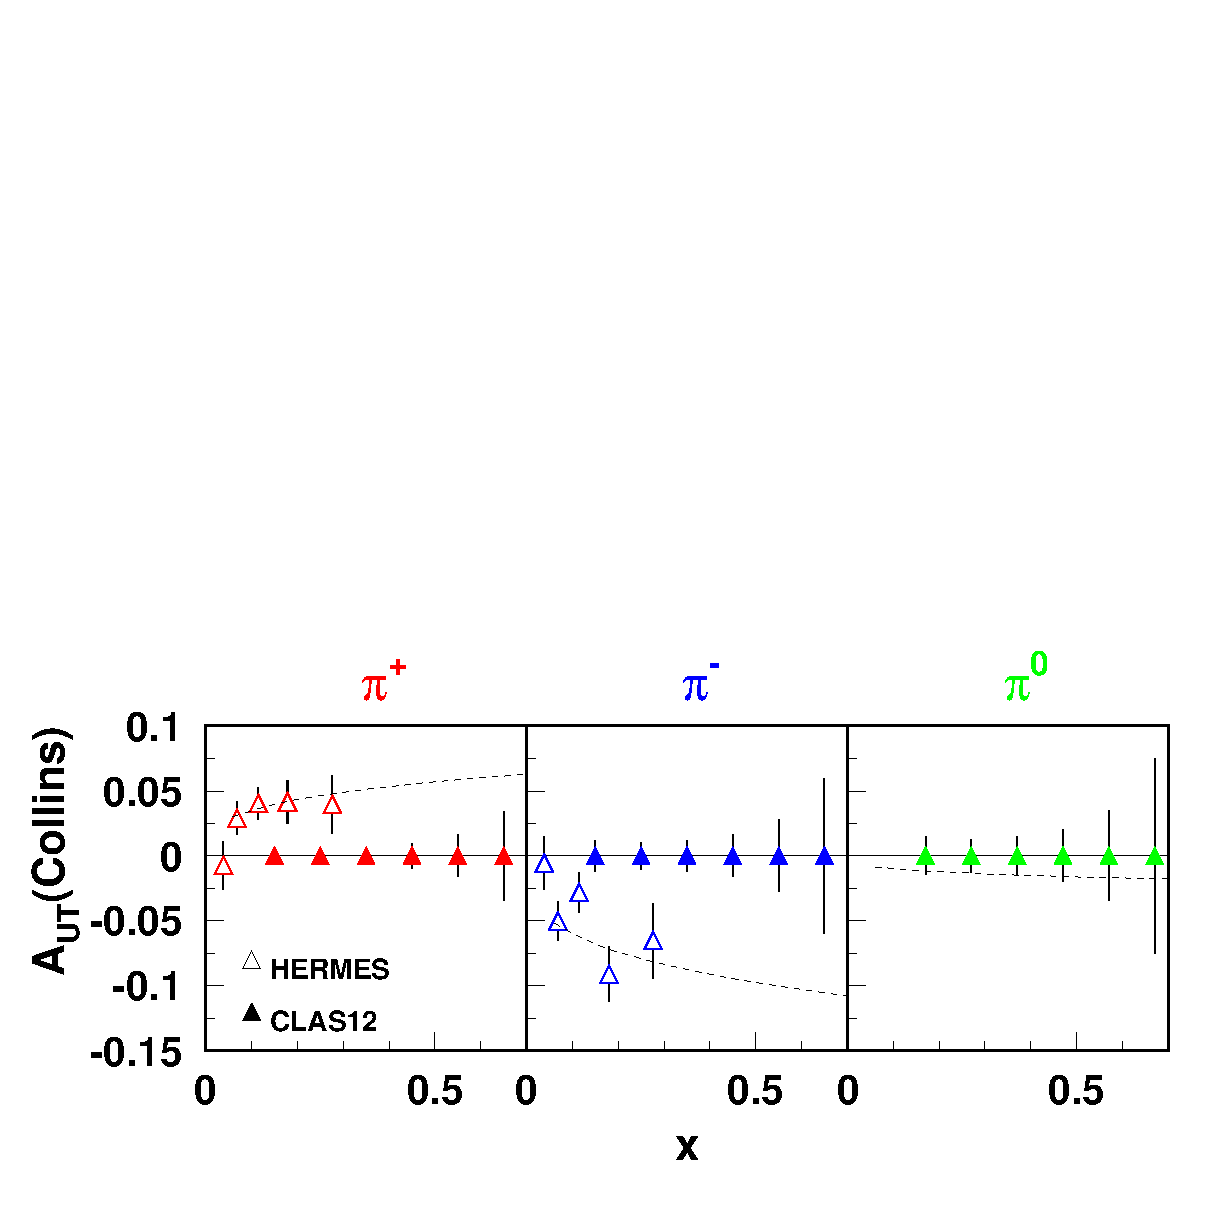
\psfig{file=../sidis/autcollins11.her.eps,height=14cm,width=14.0cm} }
\caption{\small{Projected transverse spin asymmetry from the Collins effect 
($A_{UT}^{\sin(\phi+\phi_S)}$) in single $\pi$ production with {\tt CLAS} at 
11~GeV.}} 
\label{fig:autcol}
\end{center}
\end{figure}
%%%%%%%%%%%%%%%%%%%%%%%%%%%%%%%%%%%%%%%%%%%%%%%%%%%%%%%%%%%%%%%%%%%%%%%%%%%%%

\vspace{0.2cm}\noindent

%%%%%%%%%%%%%%%%%%%%%%%%%%%%%%%%%%%%%%%%%%%%%%%%%%%%%%%%%%%%%%%%%%%%%%%%%%%%
\begin{figure}[tb]
\begin{center}
\vspace{-6.0cm}
\mbox{ 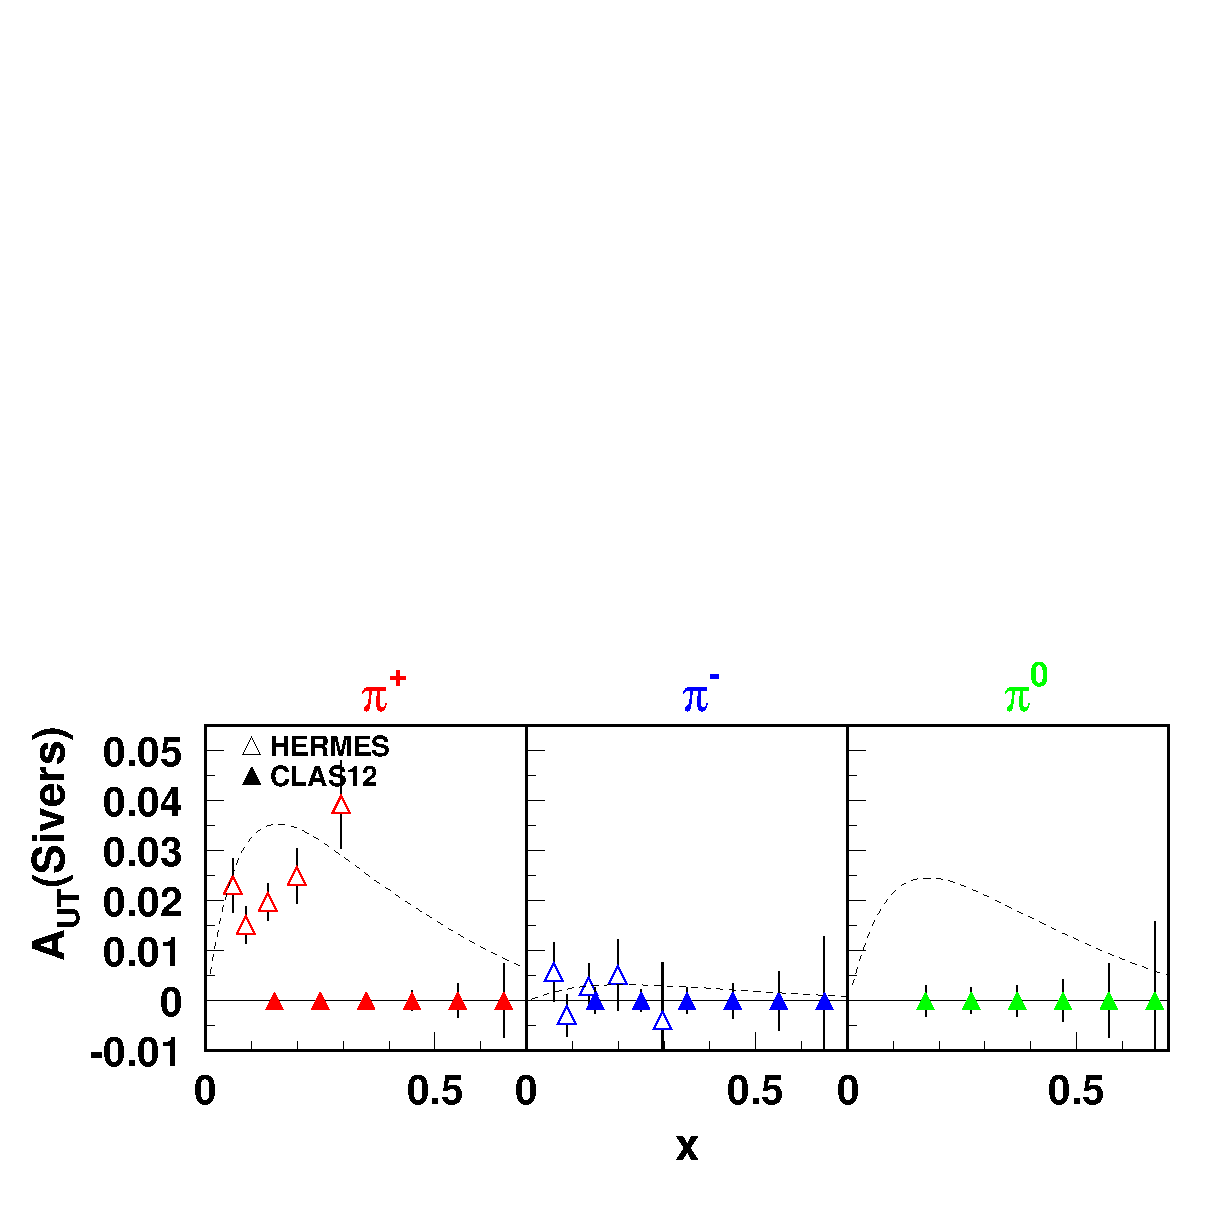
\psfig{file=../sidis/autsivers11.weiss.eps,height=14cm,width=14.0cm} }
\caption{\small{Projected transverse spin asymmetry from the Sivers effect 
($A_{UT}^{\sin(\phi-\phi_S)}$) in single $\pi$ production with {\tt CLAS12} 
at 11~GeV.}}
\label{fig:autsiv}
\end{center}
\end{figure}
%%%%%%%%%%%%%%%%%%%%%%%%%%%%%%%%%%%%%%%%%%%%%%%%%%%%%%%%%%%%%%%%%%%%%%%%%%%%

The leading-twist transversity distribution $h_1$
\cite{Ralston:1979ys,Jaffe:1991ra} and its first moment, the tensor charge, 
are as fundamental for understanding of the spin structure of the nucleon as 
are the helicity distribution $g_1$  and the axial vector charge.  The 
transversity distribution  $h_1$ is charge conjugation odd.  It does not mix 
with gluons and for non-relativistic quarks it is equal to the helicity
distribution $g_1$.  Thus, it probes the relativistic nature of quarks and it 
has a very different $Q^2$ evolution than $g_1$.  The tensor charge is 
reliably calculable in lattice QCD with $\delta \Sigma = \sum_f 
\int_0^1dx(h_1^f - \bar{h_1^f})=0.562 \pm 0.088$ at $Q^2$=2~GeV$^2$, which is 
twice as large as the value of proton axial charge~\cite{Leader:1999rh}.  A 
similar quantity ($\delta \Sigma \approx 0.6$) was obtained in the effective 
chiral quark soliton model~\cite{Kim:1996vk}. 

A detailed study of the $Q^2$ and $x_B$ dependencies as a function of the 
azimuthal angle $\phi$ will allow the separation of contributions from 
different mechanisms.  During the last few years, first results on transverse 
SSAs have become available~\cite{Airapetian:2004tw,Alexakhin:2005iw}. HERMES 
measurements for the first time directly indicated significant azimuthal 
moments generated both by Collins (Fig.~\ref{fig:autcol}) and Sivers 
(Fig.~\ref{fig:autsiv}) effects.

Spin-orbit correlations are also accessible in SIDIS with longitudinally a
polarized target, where they give rise to the Mulders leading-twist 
distribution function $h_{1L}^\perp$. It is related to the real part of
the interference of wave functions for different orbital momentum states,
and describes transversely polarized quarks in the longitudinally polarized 
nucleon.  For a longitudinally polarized target the only azimuthal asymmetry
arising in leading order is the $\sin2\phi$ moment,

\begin{equation}
\sigma^{\sin2\phi}_{UL} \propto S_L 2(1-y)\sin 2\phi\sum_{q,\bar{q}} e^2_q {x h^{\perp q}_{1L}(x)} {H_1^{\perp q}(z)}.
\end{equation}

The physics of $\sigma_{UL}$, which involves the Collins fragmentation 
function $H_1^\perp$ and Mulders distribution function $h_{1L}^\perp$, 
was first discussed by Kotzinian and Mulders in 1996 
\cite{Mulders:1995dh,Kotzinian:1994dv,Kotzinian:1995cz}.  The same 
distribution function is accessible in double polarized Drell-Yan, where it 
gives rise to the $\cos2\phi$ azimuthal moment in the cross section 
\cite{Tangerman:1994eh}.

Measurements of the $\sin2\phi$ SSA \cite{Kotzinian:1995cz}, thus allow the 
study of the Collins effect with no contamination from other mechanisms.  A 
recent measurement of the $\sin 2\phi$ moment of $\sigma_{UL}$ by HERMES 
\cite{Airapetian:1999tv} is consistent with zero.  A measurably large 
asymmetry has been predicted only at large $x$ ($x>0.2$), a region 
well-covered by JLab~\cite{Efremov:2002ut}. 

The kinematic dependence of the SSA for $\pi^+$, measured from the {\tt CLAS} 
EG1 data set at 6~GeV is consistent with predictions~\cite{Efremov:2002ut}. 
The $\pi^+$ SSA is dominated by the $u$-quarks; therefore with some assumption 
about the ratio of unfavored to favored Collins fragmentation functions, it can 
provide a first glimpse of the twist-2 Mulders TMD function.  The distribution 
function $h_{1L}^\perp$ was extracted using the $\pi^+$ target SSA 
\cite{Avakian:2005ps}, which is less sensitive to the unknown ratio of 
unfavored ($d$-quark fragmenting to $\pi^+$) to favored ($u$-quark fragmenting 
to $\pi^+$) polarized fragmentation functions (see Fig. \ref{fig:aul11.sin2}). 
The curve is the result of the calculation by Efremov {\it et al.} 
\cite{Efremov:2002ut}, using $h_{1L}^\perp$ from the chiral quark soliton 
model evolved to $Q^2$=1.5~GeV$^2$.  The extraction, however, suffers from low 
statistics and has a significant systematic error from the unknown ratio of 
the Collins favored and unfavored fragmentation functions, the unknown ratio 
of $h_{1L}^d/h_{1L}^u$, as well as from background from exclusive vector mesons.
Current statistical errors for $\pi^-$, and in particular $\pi^0$, which is 
relatively free of possible higher twist contributions \cite{Afanasev:1996mj},
are large and do not allow strong conclusions from the measured SSAs.  More 
data are required for a statistically significant measurement of the
$\sin2\phi$ moment.

The only leading-twist contribution to the unpolarized target cross section
depending on the azimuthal angle has a term with the Boer-Mulders function 
coupling to the Collins function~\cite{Collins:1992kk}:

\begin{equation}
\sigma^{\cos2\phi}_{UU} \propto 2(1-y)\cos 2\phi\sum_{q,\bar{q}} 
e^2_q {x h^{\perp q}_{1}(x)} {H_1^{\perp q}(z)}.
\end{equation}

The physics of $\sigma^{\cos2\phi}_{UU}$, which involves the Collins 
fragmentation function $H_1^\perp$ and the Boer-Mulders distribution function 
$h_{1}^\perp$, was first discussed by Boer and Mulders in 1998
\cite{Boer:1997nt}.  In recent years, the $\cos 2\phi$ asymmetry in 
leptoproduction was phenomenologically studied using different approximations 
for the Boer-Mulders function 
\cite{Oganesian:1997jq,Gamberg:2003ey,Barone:2005kt}.

Independent information on the Boer-Mulders function 
$h_1^{\perp}(x, \Vec k_T^2)$ can be obtained from the study of the $\cos 2\phi$
azimuthal asymmetry in unpolarized Drell-Yan processes, which has been
measured in $\pi N$ collisions~\cite{Falciano:1986wk,Conway:1989fs}.
In Refs.~\cite{Lu:2004hu,Lu:2005rq} this asymmetry was estimated by computing 
the $h_1^{\perp}$ distribution of the pion and of the nucleon in a quark 
spectator model~\cite{Jakob:1997wg,Bacchetta:2003rz}.  The $\cos 2\phi$ 
azimuthal asymmetry in SIDIS was computed assuming that the $\pi^+$ production 
is dominated by $u$ quarks and using the same distributions
$h_1^{\perp} (x, \Vec k_T^2)$ and $f_1 (x, \Vec k_T^2)$ used in 
Ref.~\cite{Lu:2005rq}.

The calculation of the $\cos 2 \phi$ asymmetry appeared to be in rather good 
agreement for low values of $P_T$ (up to 0.5~GeV) with SIDIS data coming 
from the ZEUS experiment~\cite{Breitweg:2000qi} at large $Q^2$ values 
($0.01<x<0.1$, $0.2<y<0.8$, $0.2<z<1$, $Q^2 > 180$ GeV$^2$) where the 
higher-twist contributions are not expected to be relevant.

It is important to note that both $\pi^+$ and $\pi^-$ azimuthal moments may
have significant contributions from exclusive vector meson production.
The fraction of $\pi^+$ in the single pion sample, coming from exclusive 
$\rho^0$ decays, is somewhat less but still significant at large $z$ and in 
particular for small $x$.  The two pion data from {\tt CLAS12} would allow us
to extract exclusive two pion asymmetries and estimate their contribution to 
the single pion SSA.

\section{TMD Measurements with JLab at 12 GeV}

Projections for target single-spin asymmetry measurements with {\tt CLAS12} 
at 11~GeV are plotted in Figs.~\ref{fig:autcol}-\ref{fig:autsiv}.  The 
projected error bars have been calculated assuming a luminosity of
$5\times 10^{34}$~cm$^{-2}$s$^{-1}$, with an $NH_3$ target polarization of 
85\% and a dilution factor of 0.14, with 2000~hours of data taking.
The asymmetry is integrated over all hadron transverse momenta.

The target single-spin asymmetry from polarized quark fragmentation
extracted for {\tt CLAS12} kinematics at 11~GeV is plotted in 
Fig.~\ref{fig:autcol}.  The estimate was done assuming $h_1 \approx g_1$ and 
an approximation for the Collins fragmentation function from 
Ref.~\cite{Efremov:2002ut}.  Additional cuts were applied on $z$ ($z>0.5$) 
and the missing mass of the $e'\pi^+$ system ($M_X(\pi^+)>1.3$~GeV). 

The extraction of the transversity from $A^{\sin\phi}_{UT}$ could be 
performed using parameterizations for the unpolarized distribution 
functions $u(x)$ and $\bar{d}(x)$ and certain approximations for the 
polarized Collins fragmentation function $H_1^{\perp}$.  The measurement of 
transversity is complicated by the presence of an essentially unknown Collins 
function.  Recently, the Collins function for pions was calculated in a chiral 
invariant approach at a low scale~\cite{Bacchetta:2002tk} and it was shown 
that at large $z$ the function rises much faster than previously predicted 
\cite{Efremov:2002ut,Kotzinian:1999dy} in the analysis using the HERMES data 
on target SSA.  It was also pointed out that the ratio of polarized and 
unpolarized fragmentation is almost scale independent~\cite{Bacchetta:2002tk}.
Significant asymmetry was measured by Belle \cite{Abe:2005zx} indicating that 
the Collins function is indeed large.  The transverse asymmetry measurements 
were performed at HERMES~\cite{Airapetian:2001eg} and COMPASS
\cite{Alexakhin:2005iw}.  The first extraction of the transversity 
distribution has been carried out recently~\cite{Anselmino:2007fs} combining 
$e^+e^-$ and semi-inclusive DIS data~\cite{Airapetian:2004tw}.  The 
statistics, however, are not enough to make statistically significant 
predictions in the valence region, where the effects are large.

Significantly higher statistics from {\tt CLAS12} data, especially in the 
large $\xbj$ region, will enable the extraction of the $\xbj$ and $Q^2$ 
dependencies for different azimuthal moments in a wide kinematic range 
allowing the source of the observed SSA to be revealed and will allow
extraction of the underlying distribution functions.

%%%%%%%%%%%%%%%%%%%%%%%%%%%%%%%%%%%%%%%%%%%%%%%%%%%%%%%%%%%%%%%%%%%%%%%%%%%
\begin{figure}[htbp]
\vspace{7.0cm}
\special{psfile=../sidis/autsivpi0.bnl.eps hscale=70 vscale=65 hoffset=30 voffset=-20}
\caption{\small{Projected transverse spin asymmetry ($A_{UT}^{\sin\phi-\phi_S}$)
in single $\pi^0$ production with {\tt CLAS12} at 11~GeV.  The curves are 
calculated using models for the Sivers function from Efremov {\it et al.}
\cite{Efremov:2004tp}, $F_{1T}=\sum_q^{u,d}e_q^2f_{1T}^{\perp q}$.}}
\label{fig:autsiv1}
\end{figure}
%%%%%%%%%%%%%%%%%%%%%%%%%%%%%%%%%%%%%%%%%%%%%%%%%%%%%%%%%%%%%%%%%%%%%%%%%%%

The measurement of the transverse asymmetry from the Sivers effect (see 
Fig.~\ref{fig:autsiv1}) with $\pi^0$ will provide a model-independent 
extraction of the Sivers function. Furthermore, measurements with proton and 
neutron targets will provide  model-independent information on flavor
partners of the Sivers function.

The transversely polarized target measurements also provide access to the 
leading-twist TMD $g_{1T}^q(x)$ appearing in convolution with the unpolarized
fragmentation function ${D_1^{q}(z)}$ in a $\cos\phi$ moment of the cross 
section.  Significant asymmetries were predicted recently for {\tt CLAS12} 
\cite{Kotzinian:2006dw} providing access also to $g_{1T}^q(x)$, describing 
longitudinally polarized quarks in the transversely polarized nucleon.
Measurements of transverse momenta of final state hadrons in SIDIS with 
longitudinally polarized targets will provide complementary to transverse 
target information, probing the longitudinal nucleon structure beyond the 
collinear approximation.  The $P_\perp$-dependence of the double-spin 
asymmetry, measured for different bins in $z$ and $x$ will provide a test of 
the factorization hypothesis and probe the transition from the non-perturbative 
to perturbative description.  At large $P_T$ ($\Lambda_{QCD}<<P_T<<Q$) the 
asymmetry is expected to be independent of $P_\perp$~\cite{Ji:2004wu}. 
There are indications that the double-spin asymmetry (see 
Fig.~\ref{a1pptdepvszq47x16}) at small $P_T$ tends to increase for $\pi^-$ 
and decrease for $\pi^+$.  A possible interpretation of the $P_T$-dependence 
of the double spin asymmetry may involve different widths of transverse 
momentum distributions of quarks with different flavor and polarization 
\cite{Anselmino:2006yc} resulting from a different orbital structure of quarks 
polarized in the direction of the proton spin and opposite to it 
\cite{Brodsky:1980zm,Brodsky:1994kg}.  This interpretation may demand a 
different width for $d$-quarks than for $u$-quarks, consistent with 
observation from lattice QCD studies of a different spread in transverse 
distances for $d$-quarks compared to $u$-quarks~\cite{Gockeler:2005cd}.
The same effect may be responsible for the relatively large $\cos\phi$ moment
of the double spin asymmetry (see Fig.\ref{a1pptdepvszq47x16}, right panel).

Detailed measurements of $A_{LL}$ and its $\cos\phi$ moment as a function 
of $P_T$ in different bins in $x,z,Q^2$ combined with measurements of
azimuthal moments of the unpolarized cross section proposed for {\tt CLAS12} 
will allow study of the flavor dependence of transverse momentum distributions.

%%%%%%%%%%%%%%%%%%%%%%%%%%%%%%%%%%%%%%%%%%%%%%%%%%%%%%%%%%%%%%%%%%%%%%%%%%%%%
\begin{figure}[htbp]
\vspace{6.8cm}
\special{psfile=../sidis/allpt11.eps hscale=42 vscale=47 hoffset=-5 voffset=-10}
\special{psfile=../sidis/allpt11cos.eps hscale=42 vscale=47 hoffset=240 voffset=-10}
\caption{\small{The double spin asymmetry $A_{LL}$ (left) and its $\cos\phi$ 
moment (right) as a function of the transverse momentum of hadrons, $P_T$,  
averaged in the $0.4<z<0.7$ range.}}
\label{a1pptdepvszq47x16}
\end{figure}
%%%%%%%%%%%%%%%%%%%%%%%%%%%%%%%%%%%%%%%%%%%%%%%%%%%%%%%%%%%%%%%%%%%%%%%%%%%%%

Projections for the resulting kinematic dependence of the leading-twist SSA  
are shown in Fig.~\ref{fig:aul11.sin2}.  Calculations were done using 
$h_{1L}^\perp$ from the chiral quark soliton model evolved to 
$Q^2$=1.5~GeV$^2$~\cite{Efremov:2002ut}, $f_1$ from GRV95~\cite{Gluck:1995yr}, 
and $D_1$ from Kretzer, Leader, and Christova~\cite{Kretzer:2001pz}. Three 
different curves correspond to $H_1^{\perp u\rightarrow \pi^+}/
H_1^{\perp u\rightarrow \pi^-}=0,-1.2,-5$~\cite{Efremov:2004hz}. Corresponding 
projected error bars for the Mulders TMD parton distribution are shown
in Fig.~\ref{fig:aul11.sin2}.  An important ingredient for the estimates are 
so-called ``Lorentz-invariance relations'' that connect $h_{1L}^{\perp}$ with 
$h_1$~\cite{Mulders:1995dh}.  Meanwhile these relations are known not to be 
valid exactly~\cite{Goeke:2003az,Goeke:2005hb}.  It is of importance to find
out experimentally to which extent such relations can provide useful 
approximations, or whether they are badly violated, since there is little 
theoretical intuition on that point.

%%%%%%%%%%%%%%%%%%%%%%%%%%%%%%%%%%%%%%%%%%%%%%%%%%%%%%%%%%%%%%%%%%%%%%%%%%%%%
\begin{figure}
\vspace{-2.0cm}
\begin{tabular}{cc}
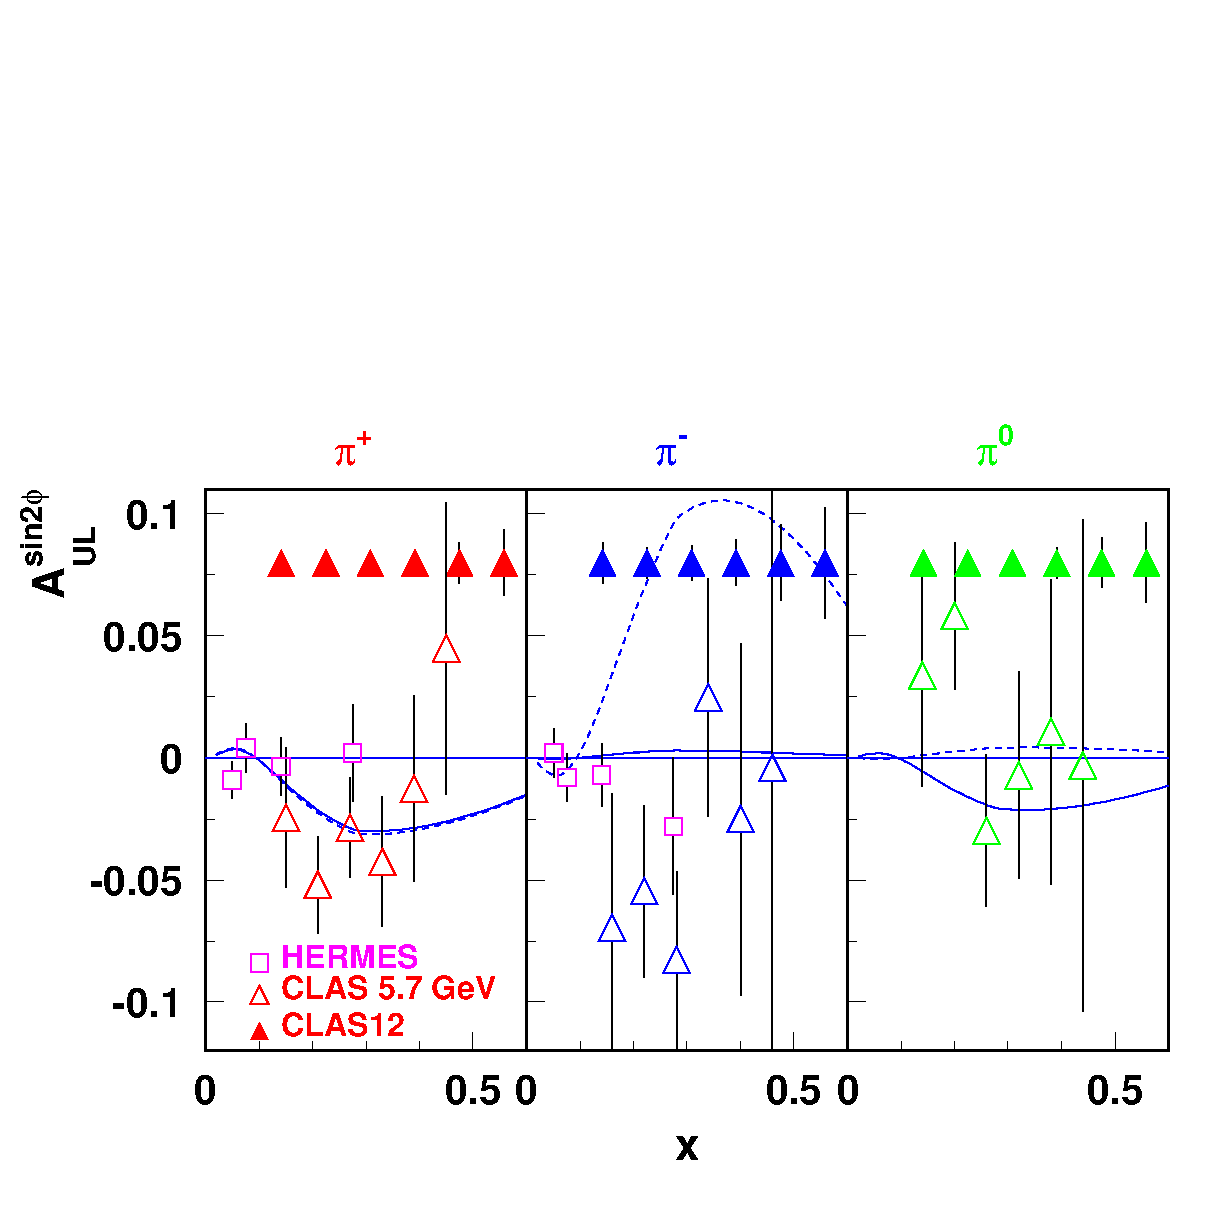
\includegraphics[height=.4\textheight,width=0.45\textwidth]{../sidis/aul11.sin2.eps}
&
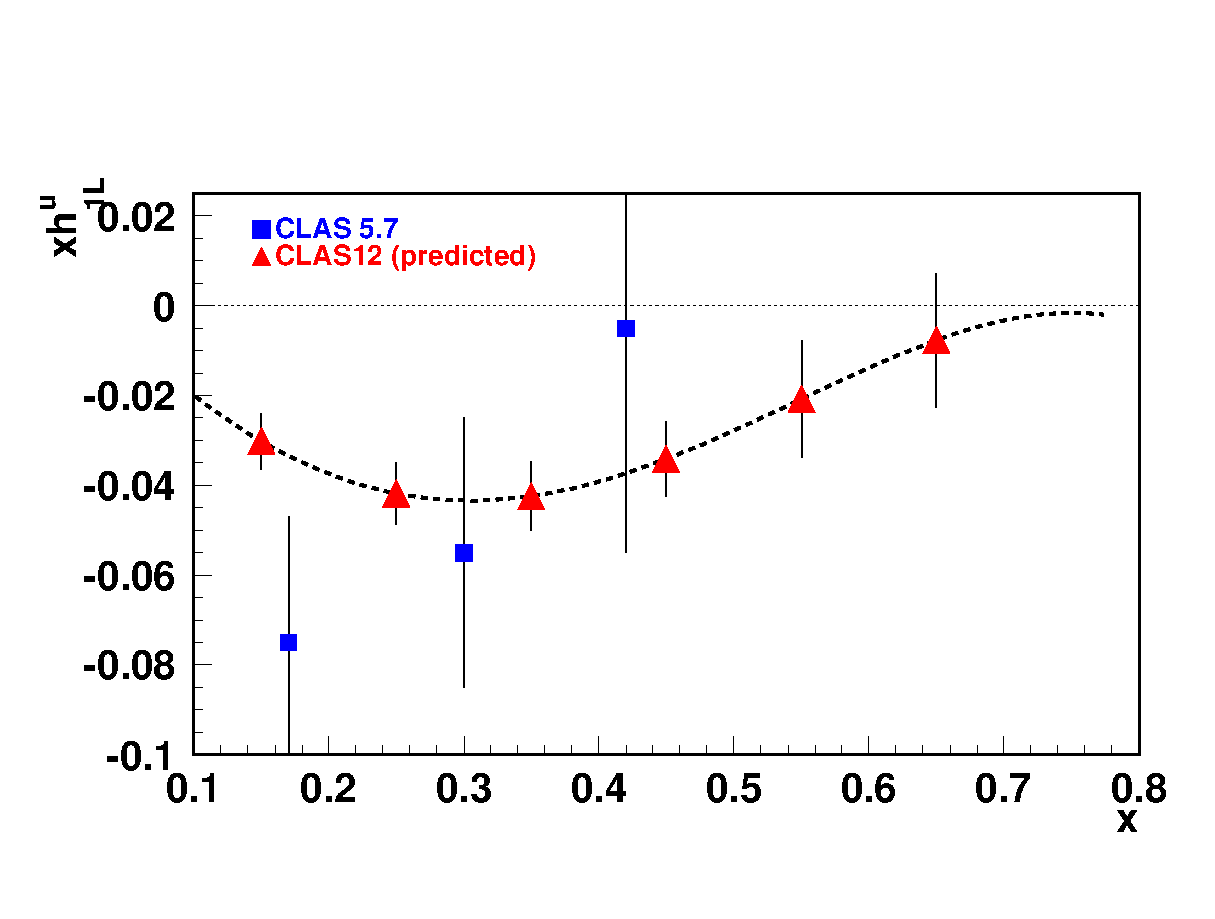
\includegraphics[height=.31\textheight,width=0.45\textwidth]{../sidis/h1lu11.eps}
\\
(a) & (b)
\end{tabular}
\caption{\small{(Left) The projected $x$-dependence of the target SSA at 
11~GeV.  The triangles illustrate the expected statistical accuracy.  The open 
squares and triangles show the existing measurement of the Mulders TMD from 
HERMES and the {\tt CLAS} 5.7~GeV EG1 data sets, respectively.  The curves 
are calculated using Ref.~\cite{Efremov:2004hz}. (Right) Projection for the
Mulders distribution function for the $u$-quark from the $\pi^+$ SSA from 
{\tt CLAS12} (predicted) compared with the {\tt CLAS} EG1 data set at 
5.7~GeV.}}
\label{fig:aul11.sin2}
\end{figure}
%%%%%%%%%%%%%%%%%%%%%%%%%%%%%%%%%%%%%%%%%%%%%%%%%%%%%%%%%%%%%%%%%%%%%%%%%%%%%

Proposed measurements of SSAs in SIDIS will pin down the corresponding TMD 
distribution and will constrain the ratio of favored to unfavored polarized 
fragmentation functions.  The new data will also allow a more precise test of 
the factorization ansatz and the investigation of the $Q^2$ dependence of  
$\sin 2\phi$, $\sin \phi$, and $\cos \phi$ asymmetries. This will enable us 
to study the leading-twist and higher-twist nature of the corresponding 
observables~\cite{Levelt:1994np,Jaffe:1991ra,Kotzinian:1999dy,Afanasev:2003ze,
Yuan:2003gu,Metz:2004je,Collins:2004nx}.

The Boer-Mulders contribution, being leading twist, is expected to survive at 
higher $Q^2$ and that can be tested at the large $Q^2$ accessible with 
{\tt CLAS12}.  At large transverse momentum, {\it i.e.} 
$P_{h\perp}\gg \Lambda_{\rm QCD}$, the transverse-momentum dependence of the 
various factors in the factorization formula~\cite{Ji:2004wu} may be 
calculated from perturbative QCD.  Following the similar arguments in 
Ji-Qiu-Vogelsang-Yuan~\cite{Ji:2006vf}, the $\cos 2\phi$ azimuthal asymmetry 
has the following behavior at $\Lambda_{\rm QCD}\ll P_{h\perp}\ll Q$,

\begin{equation}
\langle \cos 2\phi\rangle|_{P_{h\perp}\gg\Lambda_{\rm QCD}}\propto
\frac{1}{P_{h\perp}^2} \ .
\end{equation}

When the transverse momentum is compatible with the large-scale $Q$, the above 
results will be modified, because the gluon radiation from the pQCD diagram 
will dominate, and contribute to the azimuthal asymmetry not being suppressed 
by any hard scale.  At $Q^2$ values accessible at JLab ($1.0<Q^2<10$~GeV$^2$), 
however, the reduction of the Boer-Mulders asymmetry due to Sudakov form 
factors arising from soft gluon contributions~\cite{Boer:2001he} is not 
expected to be significant.

Measurement of the $P_T$ dependence of the Boer-Mulders-asymmetry (see 
Fig.~\ref{fig:aucos21mx}) will allow for checking of the predictions of a 
unified description of SSA by Ji and collaborators~\cite{Ji:2004wu,Ji:2006vf} 
and for study of the transition from a non-perturbative to a perturbative 
description.  The $\cos 2 \phi$ asymmetry for semi-inclusive deep inelastic 
scattering in the kinematic regions of {\tt CLAS12} is predicted to be 
significant (a few percent on average) and tends to be larger in 
the small-$x$ and large-$z$ region. The preliminary data from {\tt CLAS} at 
6~GeV indeed indicate large azimuthal moments both for $\cos\phi$ and 
$\cos 2\phi$.

%%%%%%%%%%%%%%%%%%%%%%%%%%%%%%%%%%%%%%%%%%%%%%%%%%%%%%%%%%%%%%%%%%%%%%%%%%%%%
\begin{figure}[htbp]
\vspace{6.9cm}
\special{psfile=../sidis/auucos21mxnew.eps hscale=60 vscale=57 hoffset=50 voffset=-5}
\caption{\small{The $\cos2\phi$ moment (Boer-Mulders asymmetry) for pions
as a function of $x$ and $P_T$ for $Q^2>2$~GeV$^2$ (right) with {\tt CLAS12} 
at 11~GeV from 2000~hours of running.  Values are calculated assuming
$H_1^{\perp u\rightarrow \pi^+}=-H_1^{\perp u\rightarrow \pi^-}$.}}
\label{fig:aucos21mx}
\end{figure}
%%%%%%%%%%%%%%%%%%%%%%%%%%%%%%%%%%%%%%%%%%%%%%%%%%%%%%%%%%%%%%%%%%%%%%%%%%%%%

The combined analysis of the future {\tt CLAS12} data on 
$\langle \cos 2 \phi \rangle$ and of the previous ZEUS measurements in the 
high-$Q^2$ domain (where higher-twist effects are negligible) will provide 
information on the Boer-Mulders function, shedding light on the correlations 
between transverse spin and transverse momenta of quarks.  Significantly 
increasing the kinematic coverage at large $Q^2$ and $P_T$, {\tt CLAS12}
(see Fig.~\ref{fig:aucos21mx}) will map the quark TMDs in the valence region
allowing study of the transition from a non-perturbative description at small 
$P_T$ to a perturbative description at large $P_T$.
 
Measured single and double spin asymmetries for all pions in a large range of 
kinematic variables ($x_B$, $Q^2$, $z$, $P_{\perp}$, and $\phi$) combined with 
measurements with unpolarized targets will provide detailed information on the 
flavor and polarization dependence of the transverse momentum distributions of 
quarks in the valence region, and in particular, on the $x_B$, $z$, and 
$P_{\perp}$ dependence of the leading TMD parton distribution functions of $u$ 
and $d$ quarks.  Such measurements across a wide range of $x$, $Q^2$, and $P_T$ 
would allow for detailed tests of QCD dynamics in the valence region 
complementing the information obtained from inclusive DIS.  They would also 
serve as novel tools for exploring nuclear structure in terms of the quark and 
gluon degrees of freedom of QCD.

\section{Summary}

In summary, with upgraded energy and luminosity, {\tt CLAS12} can study 
single- and double-spin asymmetries, involving essentially unexplored 
chiral-odd and time-odd distributions functions, including transversity
\cite{Ralston:1979ys,Jaffe:1991ra}, Sivers~\cite{Sivers:1990fh,Brodsky:2002cx,
Collins:2002kn,Ji:2002aa}, Boer-Mulers~\cite{Boer:1997nt}, and Collins
\cite{Collins:1992kk} functions, providing detailed information on the quark 
transverse momentum and spin correlations~\cite{Collins:1992kk,Kotzinian:1994dv,
Mulders:1995dh,Brodsky:2002rv,Jaffe:2002pj}.

Measurements of semi-inclusive processes combined with inclusive and 
exclusive measurements with an upgraded JLab will allow us to study the quark 
structure of the nucleon with unprecedented detail.  Understanding of 
spin-orbit correlations, together with independent measurements related to the 
spin and orbital angular momentum of the quarks, will help to construct a more 
complete picture of the nucleon in terms of elementary quarks and gluons going 
beyond the simple collinear partonic representation.


\chapter{Properties of QCD from the Nuclear Medium}

\section{Introduction}

While the strong interaction seems to be well described by QCD at high
energies, in the non-perturbative domain it remains largely unsolved
and untested. Further, little is known from experiment about the
space-time characteristics of QCD at any energy scale. Exploration of
the QCD phase diagram for hot, dense matter is a large effort in QCD
physics, and these studies can take advantage of pQCD, however, a
QCD-based description of cold, dense matter still represents a 
formidable challenge. Lattice QCD, in combination with chiral effective 
theory, will partly address the non-perturbative physics and the hot, 
dense matter, but space-time processes and non-zero baryon density are 
still inaccessible via lattice techniques.

New experimental access to a number of properties and consequences of
QCD will become available at 12~GeV. Properties of deconfined quarks,
such as their lifetimes and energy loss, can be extracted. The time
evolution of $q\bar{q}$ pairs can be deduced from studies of color
transparency. The process in which hadrons are formed out of energetic 
quarks can be characterized, both in terms of formation times and 
formation mechanisms. The properties of strongly interacting nucleons 
and their connections to cold, dense matter can be accessed with 
precision over a broad kinematic range, potentially connecting to 
astrophysical systems such as neutron stars. These are exciting 
prospects that will provide profound new insights into the space-time 
characteristics of fundamental QCD processes and the nature of cold 
QCD matter.

\boldmath
\subsection{$p_T$ Broadening and the Lifetime of Deconfined Quarks}
\unboldmath

The confinement of quarks into hadrons is the most important
manifestation of the non-Abelian character of QCD. Achieving a
quantitative understanding of confinement is one of the highest
priority endeavors of nuclear and hadronic physics, and ranks as 
one of the great quests of modern science. The effort to understand
confinement is multi-pronged, typically involving hadron spectroscopy
interpreted through the use of models and lattice calculations, which
aim to characterize the effective potential between quarks. In
addition to the effective potential, another important piece of
confinement is the process of color neutralization, wherein a
deconfined colored quark finds colored partners, such that the
resulting system is a color singlet. Experimental access to the
characteristics of the deconfined quark can be obtained using
semi-inclusive deep inelastic scattering on nuclei in specific
kinematic regions.

In deep inelastic scattering (DIS) kinematics with $x>0.1$, quark-pair 
production by the virtual photon is suppressed~\cite{DDBH} and the target 
quark absorbs all of its energy and momentum. Thus, neglecting the 
intrinsic quark momentum, the initial quark energy is $\nu$ and its 
direction is given by the direction of the virtual photon. The quark 
propagates for some distance until its color is neutralized, at which 
point it is contained in a ``pre-hadron'' that subsequently evolves into 
a fully formed hadron~\cite{KNPH}. In the event that the neutralization 
takes place outside of a nuclear target, the interactions of the struck 
quark with the nuclear medium are limited to partonic-level multiple 
scattering, primarily due to the emission of medium-stimulated gluons
\cite{XGXNW}. This multiple scattering broadens the distribution of 
momentum transverse to the virtual photon direction, which is observable 
by measurement of the final state hadron's $p_T^2$ distribution. 
Subtracting the intrinsic quark $p_T^2$ distribution as measured in 
deuterium yields the basic observable of $p_T$ broadening: 

\begin{equation}
\Delta p_T^2=p_T^2(A)-p_T^2(^2H).
\end{equation}

One property of the deconfined quark that can be accessed is its
lifetime, known as the production time $\tau_p$~\cite{SJBAHM88}. 
This is accessed by studying the dependence of $p_T^2$ on $\nu$ for 
several nuclei. Since $\tau_p$ is time dilated in proportion to $\nu$,
the $\nu$ dependence of $p_T^2$ for a series of nuclei of known
dimensions can be deconvoluted to reliably yield an estimate of
$\tau_p$. While measurements with a 5-GeV electron beam have
demonstrated the feasibility of the method~\cite{EG2,Haf06}, with an 11-GeV 
beam a much wider range in $\nu$ will be accessible. An example of a
measurement of this type is shown in Fig.~\ref{pt2}, where
$\Delta p_T^2$ is shown for three nuclei in a range of $\nu$ from 2 to
9~GeV. 

%%%%%%%%%%%%%%%%%%%%%%%%%%%%%%%%%%%%%%%%%%%%%%%%%%%%%%%%%%%%%%%%%%%%%%%%%%%
\begin{figure}[htbp]
\vspace{7.5cm}
\special{psfile=../nuclear/pt2.ps hscale=60 vscale=60 hoffset=45 voffset=-10} 
\caption{\small{A plot of $\Delta p_T^2$ vs. $\nu$ for three different 
nuclei.  Plateaus are observed in the carbon and iron targets for larger 
values of $\nu$, indicating the production length $\tau_p$ is longer than 
the full thickness of either nucleus, but still less than that of the lead 
nucleus.}}
\label{pt2}
\end{figure}
%%%%%%%%%%%%%%%%%%%%%%%%%%%%%%%%%%%%%%%%%%%%%%%%%%%%%%%%%%%%%%%%%%%%%%%%%%%

A second property of the deconfined quark is the rate of its loss of
energy due to gluon emission. This partonic energy loss has a simple
relationship to $\Delta p_T^2$ under certain simplifying assumptions.
This energy loss can be written as:

\begin{equation}
{dE\over{dx}} \approx \frac{3}{4} \alpha_s \Delta p_T^2.
\end{equation}

\noindent
This energy loss has been estimated previously using the Drell-Yan
reaction~\cite{DY1,DY2}, although theoretical ambiguities have hampered the
extraction.  In addition, energy loss by gluon radiation is the primary 
evidence for the quark-gluon liquid discovered at RHIC~\cite{RHIC} 
through the phenomenon known as jet suppression or mono-jet production
\cite{STAR}. Thus these measurements have important interdisciplinary 
connections. In a simple picture, the energy loss can be estimated
simply from data such as that shown in Fig.~\ref{pt2} from the functional 
form and the known properties of the nucleus.  A picture such as that 
shown in Fig.~\ref{pt2} implies the observation of the novel result that 
the total energy loss is proportional to the square of the distance 
traveled through the medium, a result long predicted~\cite{BDPS}.  This 
implies a coherence behavior in QCD analogous to the QED effect known as 
the Landau-Pomeranchuk-Migdal (LPM) effect, in which electron
bremsstrahlung is suppressed by coherent scattering from multiple
scattering centers~\cite{LPM1,LPM2,Migdal}. 

Models for the energy loss of quarks typically contain a parameter called 
the transport coefficient or jet quenching parameter, $\hat{q}$.  While 
difficult to calculate in lattice QCD, this parameter can be calculated 
for a hot medium~\cite{LRW} using the AdS/CFT correspondence that 
connects nonperturbative phenomena in hot, strongly coupled gauge theories 
onto calculable problems in a dual gravity theory~\cite{ADSCFT1,ADSCFT2,ADSCFT3}.
While this technique cannot be applied to a cold medium, an extrapolation 
procedure such as that employed by Baier {\it et al.}~\cite{BAIER1,BAIER2} could 
potentially extrapolate from hot to cold media. 

\boldmath
\subsection{Color Transparency and the Time Evolution of $q\bar{q}$ Pairs}
\unboldmath

The color transparency (CT) phenomenon illustrates the power of exclusive 
reactions to isolate simple elementary quark configurations.  For a hard 
exclusive reaction, such as vector meson electroproduction on the nucleon, 
the scattering amplitude at large momentum transfer is suppressed by 
powers of $Q^2$ if the hadron contains more than the minimal number of 
constituents.  This is derived from the QCD-based quark counting rules. 
Therefore, the hadron containing valence quarks only, participates in the 
scattering.  Moreover, each quark, connected to another one by hard gluon 
exchange carrying momentum of order $Q$, should be found within a distance 
of order $1/Q$. Therefore, at large $Q^2$ one selects a very special 
configuration of the hadron wave function where all connected quarks are 
close together, forming a small size color neutral configuration called 
a Point Like Configuration (PLC).  Such an object is unable to emit or 
absorb soft gluons.  Therefore, its strong interaction with the other 
nucleons becomes significantly reduced, and then the nuclear medium 
becomes more transparent.  The nucleus offers a unique laboratory to study 
quark dynamics.  Indeed, the nucleus can be used as a revealing medium of 
the evolution in time of elementary configurations in the hadron wave 
function.  The time necessary for a quark to cross distances typical of 
the confined systems is of the order of 1~fm.  By taking into account the 
relativistic time dilation factor, the characteristic time scale 
corresponds to length scales on the order of a few fm.  The only medium 
available at this scale is the nucleus, offering to us a new generation of 
experiments where the nucleus functions as bubble chamber!

Experimentally, we would like to understand this spectacular phenomenon by 
studying the hadron attenuation as it propagates through the nuclear 
medium.  These measurements will allow us to not only access the special 
configuration of the hadron wave function, but also to study how this 
configuration dresses with time to form the fully complex asymptotic wave 
function of the hadron.  This puts us in the heart of the dynamics of 
confinement.  Furthermore, the onset of CT is related to the onset of 
factorization, which is an important requirement for accessing Generalized 
Parton Distributions (GPDs) in deep exclusive meson production. The 
$\rho^0$ meson is our hadron of choice because it offers many advantages. 
It is believed that the onset of CT is expected at lower $Q^2$ in the 
($q\bar{q}$) system than in the ($qqq$) system, as it is much more probable 
to produce a small-size system of two quarks than one of three quarks
\cite{Blat}.  In addition, the $\rho^0$ is a vector meson similar to 
the virtual photon. Therefore its production mechanism is fairly well 
understood because the virtual photon fluctuates into a ($q\bar{q}$) pair 
which then materializes into the $\rho^0$ meson. The size of the 
produced ($q\bar{q}$) can be directly connected to the virtuality of the 
photon. Therefore, smaller sizes can be reached at larger $Q^2$.

More than two decades of experimental investigations have lead to only 
one clear signal of CT at high energies.  It was observed in experiment 
E791~\cite{Aita} at Fermilab.  The $A$-dependence of the diffractive 
dissociation into di-jets of 500~GeV pions scattering coherently from 
carbon and platinum targets was measured.  It was found that the cross 
section can be parameterized as $\sigma = \sigma_{0} A^{\alpha}$, with 
$\alpha$ = 1.6.  This result is quite consistent with theoretical 
calculations~\cite{Bert1,Bert2,Bert3} including CT and obviously 
inconsistent with a cross section proportional to $A^{2/3}$, which is 
typical of inclusive pion-nucleus interactions.  At moderate energies, 
the situation is more complicated.  No evidence of CT was found in 
quasi-free $A(e,e'p)$ reactions~\cite{eep1,eep2,eep3,eep4} even for $Q^2$ 
values as large as 8~GeV$^2$.  While the outcome of quasielastic $(p,2p)$ 
scattering from nuclei~\cite{p2p1,p2p2,p2p3} 
was very controversial due to the fact that the results do not support a 
monotonic increase in transparency with $Q^2$ as predicted by CT, the 
transparency increases for $Q^2$ from 3 to 8~GeV$^2$, but then decreases 
for higher $Q^2$, up to 11~GeV$^2$.  This subsequent decrease was 
explained as a consequence of soft processes that interfere with 
perturbative QCD in free $pp$ scattering but which are suppressed in the 
nuclear medium~\cite{ral}.  Other measurements studied the attenuation 
of the $\rho^0$ vector meson in the nuclear medium via exclusive $\rho^0$ 
lepto-production off nuclei.  The results from the two measurements
\cite{meso1,meso2} are very suggestive of a CT signal, but they are 
statistically limited.

The exclusive, diffractive, incoherent electroproduction of vector mesons 
off nuclei has been suggested~\cite{kop02} as a sensitive way to detect 
CT.  In the laboratory frame, the photon fluctuation can propagate over 
a distance $l_c$ known as the coherence length.  The coherence length can 
be estimated relying on the uncertainty principle and Lorentz time dilation 
as $l_c = 2 \nu/(Q^2 + M^2_{q\bar{q}})$, where $\nu$ is the energy of the 
virtual photon in the laboratory frame, (-$Q^2$) is its squared mass, and 
$M_{q\bar{q}}$ is the mass of the ($q\bar{q}$) pair.  In the case of 
exclusive $\rho^0$ electroproduction, the mass of the ($q\bar{q}$) is 
dominated by the $\rho^0$ mass.  The produced small-size, colorless 
hadronic system will then propagate through the nuclear medium with 
reduced attenuation because its cross section is proportional to its size. 
The effect of the nuclear medium on the particles in the initial and final 
states can be characterized by the nuclear transparency $T_A$.  $T_A$ is 
defined as the ratio of the measured exclusive cross section to the cross 
section in the absence of initial and final state interactions.  It can be 
measured by taking the ratio of the nuclear per-nucleon ($\sigma_A/A$) to 
free nucleon ($\sigma_N$) cross sections:

\begin{equation}
T_A = \frac{\sigma_A}{A\sigma_N}.
\end{equation}

The signal of CT would be an increase of the nuclear transparency as 
$Q^2$ increases.  It was shown by the HERMES collaboration~\cite{acker} 
that the nuclear transparency increases when $l_c$ varies from long to 
short compared to the size of the nucleus.  This is due to the fact that 
the nuclear medium seen by the ($q\bar{q}$) fluctuation becomes shorter. 
Thus the ($q\bar{q}$) pair interacts less.  This situation occurs when 
$Q^2$ increases at fixed $\nu$.  This so-called coherence length effect 
(CL) can mimic the CT signal.  Therefore one should keep $l_c$ fixed while 
measuring the $Q^2$ dependence of the nuclear transparency.

{\tt CLAS12} is the ideal detector for such measurements.  It offers large 
acceptance, good particle identification, and high luminosity. Using 
an 11-GeV electron beam, one can extend the $Q^2$ region up to
5.5~GeV$^2$. An indication of the quality of the data that can be
obtained is shown in Fig.~\ref{res}. 
The nuclear transparency for several targets (C, Fe, and Sn) could be 
measured.  This is important in order to study the formation time of the 
hadron as it propagates through different nuclear sizes.  These 
measurements would also be a natural extension of a previous {\tt CLAS} 
experiment~\cite{koko}, where the preliminary results indicate a clear 
evidence of a CT signal despite the limited $Q^2$ range to 2~GeV$^2$.

%%%%%%%%%%%%%%%%%%%%%%%%%%%%%%%%%%%%%%%%%%%%%%%%%%%%%%%%%%%%%%%%%%%%%%%
\begin{figure}[htbp]
\vspace{9.0cm}
\special{psfile=../nuclear/tr_err_fe.eps hscale=70 vscale=65 hoffset=40 voffset=0}
\caption{\small{A plot indicating the expected error bars for the 11-GeV 
measurements of nuclear transparency for $\rho_0$ production on Fe from 
incoherent $\rho$ electroproduction (12 days of beam time), and the 
predictions of Ref.~\cite{kop02}.}}
\label{res}
\end{figure}
%%%%%%%%%%%%%%%%%%%%%%%%%%%%%%%%%%%%%%%%%%%%%%%%%%%%%%%%%%%%%%%%%%%%%%%

\section{Hadron Attenuation and the Formation Time of Color Fields}

In the preceding discussion, the focus was on the kinematics in which the 
color of the quark is neutralized outside the nucleus.  In those kinematics 
one learns about the properties of the propagating quark through its 
partonic-level multiple scattering in the medium. In this section the focus 
is on the case when the color neutralization happens within the nuclear 
medium, creating a color singlet object referred to as a pre-hadron. The 
pre-hadron evolves to a full hadron over a period of time $\tau_f$, the 
formation time.  The pre-hadron and the final hadron can both interact with 
the nuclear medium and the most probable interaction is a highly inelastic 
reaction. Relative to the same kinematics on deuterium, in a heavy nucleus 
these interactions move hadron flux at high energies to lower energies (or
lower $z$) and higher multiplicities. This is referred to as hadron 
attenuation. It is quantitatively measured by the hadronic multiplicity 
ratio $R_M^h$:
    
\begin{equation}
R_M^h = \frac{(N_h^{DIS,A})/(N_e^{DIS,A})}
{(N_h^{DIS,^2H})/(N_e^{DIS,^2H})},
\end{equation}

\noindent
where $N_h^{DIS,A}$ is the number of hadrons of species $h$ produced
in DIS kinematics on nucleus $A$, $N_e^{DIS,A}$ is the number of DIS
electrons from nucleus $A$, and the denominator refers to the same
quantities for deuterium $^2H$~\cite{HERMES}. $R_M^h$ may in principle
depend on a number of kinematic variables such as $Q^2$, $\nu$, $z$,
$p_T$, and $\phi$. Isolating the multi-variable dependence of $R_M^h$
is a powerful discriminator between models based on different physical
pictures. At the current time, two different physical pictures
dominate model descriptions. The first~\cite{WANG,ARLEO} assumes that 
hadronization takes place outside the nucleus. The second
\cite{KNPH,MOSEL} assumes that hadronization can take place inside the 
nucleus, and cite the interaction of the pre-hadron as the main cause of 
the attenuation.  Both approaches provide adequate descriptions of the 
HERMES data, which is statistics limited to one or at most two dimensional
analyses. A full multi-dimensional analysis spanning a wide kinematic
range is feasible with {\tt CLAS12}, and such an analysis will be certain 
to strongly constrain theoretical descriptions. In addition to spanning a
range of kinematic variables, it is feasible to measure a wide range
of hadron masses with varied flavor content, as may be seen in
Table~\ref{table:hadron_list}, which lists hadrons with $c\tau$ greater
than nuclear dimensions for which measurements with {\tt CLAS12} are
feasible. With a dataset of this quality and breadth, a comprehensive
program to extract hadron formation lengths is practical to carry
out. Such a program will yield insights into the systematic behavior
of how hadrons form, a heretofore unknown sector of nonperturbative
QCD in the spacetime domain.  

%%%%%%%%%%%%%%%%%%%%%%%%%%%%%%%%%%%%%%%%%%%%%%%%%%%%%%%%%%%%%%%%%%%%%%%
\begin{table}[htbp]
\begin{center}
\begin{tabular}{||c|c|c|c|c|c||} \hline \hline
hadron & $c\tau$ & mass & flavor  & detection & Production rate\\
       &         &(GeV) & content &  channel &  per 1k DIS events\\ \hline \hline
$\pi^0$ & 25 nm & 0.13 & $u\bar{u}d\bar{d}$ & $\gamma\gamma$ & 1100 \\ \hline
$\pi^+$ & 7.8 m & 0.14 &   $u\bar{d}$ & direct & 1000 \\ \hline
$\pi^-$ & 7.8 m & 0.14 &   $d\bar{u}$  & direct & 1000 \\ \hline
$\eta$ & 0.17 nm & 0.55 & $u\bar{u}d\bar{d}s\bar{s}$&$\gamma\gamma$ & 120 \\ \hline
$\omega$ & 23 fm & 0.78 &  $u\bar{u}d\bar{d}s\bar{s}$ & $\pi^+\pi^-\pi^0$ & 170 \\ \hline
$\eta'$ & 0.98 pm & 0.96 &  $u\bar{u}d\bar{d}s\bar{s}$ & $\pi^+\pi^-\eta$ & 27 \\ \hline
$\phi$ & 44 fm & 1.0 &  $u\bar{u}d\bar{d}s\bar{s}$ & $K^+K^-$ & 0.8 \\ \hline
$f1$ & 8 fm & 1.3 &  $u\bar{u}d\bar{d}s\bar{s}$ & $\pi\pi\pi\pi$ & - \\ \hline
$K^+$ & 3.7 m & 0.49 &  $u\bar{s}$ & direct & 75 \\ \hline
$K^-$ & 3.7 m & 0.49 &  $\bar{u}s$ & direct & 25 \\ \hline
$K^0$ & 27 mm & 0.50 &  $d\bar{s}$ & $\pi^+\pi^-$ & 42 \\ \hline
$p$ & stable & 0.94 &  $ud$ & direct & 530 \\ \hline
$\bar{p}$ & stable & 0.94 &  $\bar{u}\bar{d}$ & direct & 3 \\ \hline
$\Lambda$ & 79 mm & 1.1 &  $uds$ & $p\pi^-$ & 72 \\ \hline
$\Lambda(1520)$ & 13 fm & 1.5 &  $uds$ & $p\pi^-$ & - \\ \hline
$\Sigma^+$ & 24 mm & 1.2 &  $us$ & $p\pi^0$ & 6 \\ \hline
$\Sigma^0$ & 22 pm & 1.2 &  $uds$ & $\Lambda\gamma$ & 11 \\ \hline
$\Xi^0$ & 87 mm & 1.3 &  $us$ & $\Lambda\pi^0$ & 0.6 \\ \hline
$\Xi^-$ & 49 mm & 1.3 &  $ds$ & $\Lambda\pi^-$ & 0.9 \\ \hline \hline	
\end{tabular}
\end{center}
\caption{\small{Final-state hadrons potentially accessible for formation 
length and transverse momentum broadening studies in {\tt CLAS12}. The 
rate estimates were obtained from the LEPTO event generator for an 11-GeV 
incident electron beam. (The criteria for selection of these particles 
was that $c\tau$ should be larger than the nuclear dimensions, and their 
decay channels should be measurable by {\tt CLAS12}.)}}
\label{table:hadron_list}  
\end{table}
%%%%%%%%%%%%%%%%%%%%%%%%%%%%%%%%%%%%%%%%%%%%%%%%%%%%%%%%%%%%%%%%%%%%%%%

\boldmath
\subsection{$D(e,e'p_s)$ and the Quark Structure of Neutrons in a Cold
Dense Medium}
\unboldmath

For a complete understanding of QCD at hadronic scales, we need to 
learn more about the interplay between the internal (quark) structure 
of nucleons and the interaction between two nucleons. In particular, it 
is of high interest whether nucleons in close proximity to each other
(effectively at non-equilibrium high density) change their internal 
structure or perhaps even lose their separate identity to fuse into a 
``six quark cluster''~\cite{Carlson}.  Some less dramatic modifications 
of the nucleon structure that have been proposed include off-shell 
effects~\cite{MT}, $Q^2$ rescaling effects, and the suppression of
small-size configurations (PLCs) in the nucleon wave function
\cite{FS81,FS85}.  Deuterium is the optimal system to study such 
``tightly bound pairs'', since there are no additional nucleons 
interacting with the pair under study and the pair is at rest in the lab, 
with completely defined kinematics.  While the probability for a small 
inter-nucleon distance configuration in deuterium is rather small 
compared to heavier nuclei, such configurations can be ``tagged'' by the 
emission of a fast proton in the backward hemisphere relative to the 
momentum transfer vector.  We therefore propose to measure the reaction 
$D(e,e'p_b)X$ with coincident detection of the scattered electron in the 
forward part of {\tt CLAS12} and the fast (above 300~MeV) backwards 
proton in the central detector.

In the simple spectator picture, the backwards-moving proton does not 
participate in the scattering process and can serve as a tag of the 
initial state momenta of both nucleons.  By measuring the momentum of
this backward proton, we can correct the observed electron kinematics 
for the initial motion of the unobserved struck neutron and extract the 
modified neutron structure function $F_2^{n(eff)}(x, Q^2, p^2)$.
The emphasis here is not on nearly on--shell neutrons, but rather on
the opposite kinematic extreme of fast--moving neutrons, where off-shell
effects and other internal structure changes are much more pronounced.
We can extract the dependence of the structure function 
$F_2^{n(eff)}(x, Q^2, p^2)$ at fixed $x$ and $Q^2$ on the spectator
momentum $p$ in the range from about 70~MeV to 700~MeV.  We will 
simultaneously cover a large range in $x$ and $Q^2$, allowing us to make 
detailed comparisons with the different models mentioned above, including 
the rather striking change in the shape of the structure function $F_2$ 
predicted for a non-trivial six quark configuration~\cite{Carlson}.

For the proposed experiment, we will use {\tt CLAS12} in the standard
configuration, with a liquid-deuterium target and the fully 
instrumented central detector to tag the backward proton. We estimated 
the expected number of counts for a 20-day run with full luminosity
(10$^{35}$ cm$^{-2}$s$^{-1}$). The results are shown in Fig.~\ref{deeps}
as a function of the ``ordinary'' Bjorken variable $x = Q^2/2m\nu$
in the lab and for several bins in the light cone fraction $\alpha$ of
the backward proton. One can clearly see the kinematic shift due to the 
motion of the struck neutron, which we can fully correct using the proton 
kinematics.  We clearly will have good statistics for a large range in 
$x$ and in $\alpha$ (the highest bin corresponds to more than
600~MeV momentum opposite to the direction of the $q$ vector),
drastically extending the kinematic coverage and statistical precision
of the existing data from the analog experiment at 6~GeV (E94-102)
\cite{e94102}.

%%%%%%%%%%%%%%%%%%%%%%%%%%%%%%%%%%%%%%%%%%%%%%%%%%%%%%%%%%%%%%%%%%%%%%%
\begin{figure}[htbp]
\vspace{8.6cm}
\special{psfile=../nuclear/deeps.eps hscale=65 vscale=55 hoffset=35 voffset=-15}
\caption{\small{Kinematic coverage in Bjorken--$x$ and proton light-cone 
fraction $\alpha_S$ for the proposed experiment. The count rates have
been estimated for a 20-day run with the standard {\tt CLAS12} 
configuration.}}
\label{deeps}
\end{figure}
%%%%%%%%%%%%%%%%%%%%%%%%%%%%%%%%%%%%%%%%%%%%%%%%%%%%%%%%%%%%%%%%%%%%%%%

\section{$x>1$ and the Properties of Cold Dense Matter} 

Measurements with $x>1$ have been demonstrated to provide insight into
the properties of nucleon-nucleon correlations~\cite{EGIYAN,ARRINGTON}. 
With {\tt CLAS12}, the combination of increased luminosity and large 
acceptance promises to permit investigation of the hadronic final states 
associated with $x>>1$, which means that the properties of cold nuclear 
matter fluctuating ephemerally to conditions of high density can be 
accessed experimentally.  Together with theoretical extrapolations to 
equilibrium conditions, one can hope to explore such exotica as stable 
strange matter as an equilibrium component of neutron stars. A
possible experimental avenue to explore these ideas is to measure
strangeness production on a series of nuclei in $x>1$ kinematics. A
significant enhancement in kaon production increasing with $x$ may be
a signature that can be connected to equilibrium conditions at high
nuclear density which have a persistent strangeness component. These
studies complement investigations in heavy-ion reactions~\cite{GSI}
where kaon yields have recently been shown to be consistent with
thermal production in high-density nuclear matter. These exclusive or
semi-inclusive studies with $x>1$ are the natural next step following
the inclusive experiments to date. 

\subsection{The Polarized EMC Effect and the Quark Structure of Nuclei}

The well known ``EMC effect'', which shows a modification of the
$F_2$ structure function in nuclei relative to the proton, has been
a puzzle for over two decades.  Nearly 1000 papers have been written
on the subject to try to explain the EMC effect and its associated
phenomena.  The best models generally use a modification of the nucleon 
structure within the nuclear medium to explain the effect.  It is
known from lattice QCD that the region surrounding a baryon or a meson
has a suppressed chiral condensate, and it is reasonable to infer that
the nuclear medium continues this pattern.  In a quantum field theory
picture of the nucleus, the structure of bound baryons is dominantly
affected by the scalar field of the nucleus, which essentially
polarizes the nucleon and modifies its structure, particularly that of
the lower component of the relativistic wave function.  Calculations of
the polarized EMC effect indicate it is approximately twice as big as
the unpolarized effect~\cite{CLOET}.  A plot indicating the achievable
uncertainties is shown in Fig.~\ref{p_emc}.

%%%%%%%%%%%%%%%%%%%%%%%%%%%%%%%%%%%%%%%%%%%%%%%%%%%%%%%%%%%%%%%%%%%%%%%
\begin{figure}[htbp]
\vspace{6.5cm}
\special{psfile=../nuclear/REMC.eps hscale=60 vscale=60 hoffset=70 voffset=-15}
\caption{\small{A plot of the polarized EMC effect for an 11-GeV beam, 40\% 
target polarization, 80\% beam polarization, and 70 PAC days measured in 
{\tt CLAS12}. The two curves are for the two dominant structure function 
multipoles for this ($J^{\pi}=3/2^-$) nucleus; the solid line is for $K=1$ 
and the dashed line is for $M=J$.}}
\label{p_emc}
\end{figure}
%%%%%%%%%%%%%%%%%%%%%%%%%%%%%%%%%%%%%%%%%%%%%%%%%%%%%%%%%%%%%%%%%%%%%%%

\chapter{Spectroscopy}

\section{Introduction}

Spectroscopy of hadrons (mesons and baryons) is one of the key tools
for studying the theory of strong interactions, Quantum Chromodynamics 
(QCD), in the non-perturbative ({\it i.e.} confinement) regime. Hadron 
spectroscopy has been an essential component of the physics program with 
{\tt CLAS}~\cite{clas3pi,clas-d,clas-p,Tho01,McN04,Pri04,Guo07,5st}. To 
date, a large amount of experimental data on electromagnetic production of 
hadrons has been collected by {\tt CLAS}. However, more data will be 
necessary to guide improvements in hadronic phenomenology and to compare 
with lattice QCD calculations.

The majority of the data obtained so far with {\tt CLAS} is restricted to
the lowest mass states formed with the lightest quarks, up, down, and 
strange. A complete picture of QCD in the strong-coupling (non-perturbative) 
regime requires extension of hadron spectroscopy studies to higher masses 
and/or higher transferred momenta. Fulfillment of this task requires 
upgrading the electron beam energy to about 12~GeV, along with the necessary 
upgrade of the detector package, with a large-acceptance spectrometer being 
an obvious choice for studies of multi-particle final states.

The key experiments in hadron spectroscopy that we plan for the upgraded 
{\tt CLAS} detector ({\tt CLAS12}) will study reactions produced by both 
quasi-real and virtual photons.  They include:

\begin{itemize}

\item Studies of high-mass mesonic states (consisting of ordinary mesons, 
hybrids, and mesons with exotic $J^{PC}$) using H$_2$ and light nuclear 
targets;

\item Higher mass baryon production, {\it e.g.} $\Sigma$ and $\Xi$ baryons; 

\end{itemize}

Along with traditional bremsstrahlung photon beams, we are planning to 
use quasi-real photons produced when electrons are scattered at very 
forward angles ({\it i.e.} scattering angles $<$1.5$^\circ$). We plan to 
use a small-angle forward electron tagger in coincidence with the detection 
of multi-particle final states with the {\tt CLAS12} detector to study 
electroproduction at $Q^2$ values of $<10^{-2}$~GeV$^2$.  
{\it Electroproduction at these very small values of $Q^2$ using 
unpolarized electrons is equivalent to photoproduction using partially 
linearly polarized photons}~\cite{Dom69}.

The physics program using the very small-angle electron scattering
facility will take advantage of polarized photons and relatively high
photon fluxes. The use of high precision, high intensity electron beams 
will allow us to achieve the required luminosities on very thin targets 
({\it i.e.} gas targets) without jeopardizing the signal to accidental 
ratio. In turn, this will allow detection of low-energy recoils ({\it e.g.} 
coherent scattering experiments) and spectators ({\it e.g.} scattering 
off of the neutron in the deuteron). High-flux, linearly polarized
photon beams, together with the use of the nearly $4\pi$ coverage for 
hadronic final states of {\tt CLAS12}, will allow the study of hadron 
spectroscopy in a competitive and complementary experimental environment 
to the already planned {\tt GlueX} coherent bremsstrahlung production 
experiment in Hall D.

\section{Physics Motivation}

Perhaps the most fundamental question of interest to hadron physicists
is that of understanding the mechanism of confinement. It has been more
than thirty years since QCD was postulated as the theory of strong
interactions.  While much progress has been made in understanding
perturbative phenomena, the non-perturbative regime, the regime of
hadrons, their excitations, and their couplings, has remained largely
impervious to our varied assaults.  Only recently, with improvements 
to calculations of lattice QCD, has it become possible to make 
predictions of the spectrum of hadrons~\cite{morningstar,mathur}
directly from QCD, based on very few parameters (such as the bare quark 
masses). New experimental efforts to determine the hadron spectra are 
timely and are important for theoretical progress in non-perturbative QCD.

In order for this lattice effort to make significant progress in addressing 
confinement, and in order for this investment to pay off, lattice 
calculations for the masses and couplings of baryons and mesons must be 
compared with information extracted from precision experiments. Lattice 
QCD is not only capable of studying masses of bound systems of quarks 
and gluons, but it can also give insight into a space-time picture of 
electromagnetic interactions of these systems through studying the $Q^2$ 
dependence of electro-excitation form factors. We can have confidence that 
lattice calculations are indeed simulating QCD only when it successfully
reproduces a wide range of hadron properties. Some of the precision
experiments needed have been, and are being, carried out at Jefferson
Lab, and at other facilities around the world.

While mesons and baryons may be viewed differently, their phenomenology 
reflects common aspects of strong interaction dynamics. Searching for 
mesons with exotic quantum numbers gives us an opportunity to capture 
gluons as constituent particles that have their own identity, along with 
quarks, in forming hadronic bound states. On the other hand, considering 
interactions between three quarks in a baryon, one finds that the presence 
of meson-type quark correlations may be crucial in describing baryon 
properties, reflecting fundamental features of the QCD vacuum. In addition, 
multi-quark configurations in baryons are possible.

A number of legitimate questions about why this research is important
might be asked. For instance, some may question the need for more
experiments in hadron spectroscopy, since many experiments have already
addressed some of the issues discussed here. However, the experimental
coverage is incomplete. Many individual experiments have been carried out
with the aim of addressing single aspects of hadron phenomenology. Like a
map drawn by many hands, the picture of hadrons that has emerged is
incomplete in some areas, and inconsistent in others.  The goal of further
experimentation in this area is compelling: to continue our efforts to
arrive, as far as possible, at a clear, complete, and consistent
description of hadrons and their properties.

In order to understand the dynamics of QCD in the confinement region, a 
systematic study of many states, including their couplings to other states, 
is needed. Many of the current experiments at JLab, in combination with a 
systematic analysis effort, will have (in principle) information primarily 
on non-strange baryons, the nucleons and the Deltas. This information is 
not sufficient for us to arrive at a complete and consistent picture of 
the dynamics of QCD in the confinement region. Information on hyperons is
a crucial element needed for constructing such a picture. For instance,
the SU(3) singlet $\Lambda$s play key roles in identifying the states of
the 70-plets and the 20-plets.  At present, only one paper from {\tt CLAS} 
on the excited $\Lambda^*$s~\cite{barrow} has been published, and 
this study was statistically limited by the low production cross 
sections at the currently available beam energies.  Other studies of the 
excited hyperon states are in progress at {\tt CLAS} and further work can 
be done with the availability of higher energies. 

Some information on hyperons can be extracted from ongoing experiments,
but the kinematic reach of the current JLab accelerator at present does 
not allow the kind of systematic study that is essential.  The higher 
energies provided by the upgraded facility will allow for more detailed 
analysis of the spectrum and interactions of the hyperons, through 
processes like $\gamma N \to K \bar{K} N$ and $\gamma N \to KK\Xi$. 

The proposed {\tt CLAS12} experimental program is in step with current 
developments in hadronic phenomenology and lattice QCD, where the main 
thrust is a comprehensive study of the spectrum of conventional hadrons,
along with hybrid and exotic mesons and baryons. 

\section{Meson Spectroscopy}

A complete mapping of meson resonances in the mass region of 1 to 3~GeV
will be particularly important for a better understanding of the QCD 
confinement mechanism. QCD predicts the existence of several new types 
of states beyond the naive quark model, {\it e.g.}: glueballs, hybrids, 
and multi-quark $q\bar{q} q\bar{q}$ states~\cite{Is85,Ko85}.  Gluons play 
a central role in strongly interacting matter -- quark confinement is due 
to gluonic forces. The clearest most fundamental experimental signature for 
the presence of dynamics of gluon degrees of freedom is the spectrum of 
gluonic excitations of hadrons. Gluonic excitations of mesons with 
``exotic'' quantum numbers, {\it i.e.} quantum numbers not accessible 
to the $q\bar{q}$ system, would be the most direct evidence for these
states. Determining the properties of such states would shed light on
the underlying dynamics of quark confinement.

The identification of these states has been difficult, as high-mass
resonances are generally broad and overlapping, and often have similar
quantum numbers (mixing). Photoproduction cross sections are small, so
statistics have been limited. Ideally, for a complete mapping of the
mesons in this mass region, we will need to study each resonance
through as many decay channels and production mechanisms as possible
in order to disentangle mixing. To determine meson quantum numbers, we
use partial wave analysis (PWA) (in a broad sense, fits to the angular
distributions of final states). A complete PWA requires high event
statistics, as well as high resolution and geometrical acceptance of
the detector. Meson spectroscopy at {\tt CLAS12}, using the low-$Q^2$ 
tagger, will fulfill many of these stipulations.

\subsection{Coherent Photoproduction on Light Nuclei}
\label{he4}

In the electromagnetic production of $t$-channel meson resonances
at moderate energies, the main physics background arises from
associated production of baryon resonances that decay into the same
final state particles.  Often these particles in both production reactions
occupy the same phase space, and therefore, it becomes impossible to
separate them using kinematic cuts. The contribution of baryon
resonances to the final state makes PWA analysis rather complicated. The 
production of meson resonances coherently on nuclear targets, when the
recoiling nucleus remains intact, is a {\it clean} way to eliminate
baryon resonances. A particular case of such processes is coherent 
production off of light nuclei, {\it e.g.} $^3$H, $^3$He, and $^4$He. For
these reactions, the recoiling nuclei can be detected in order to ensure 
that they remain intact.

We propose a program to study charged and neutral meson resonances in
the coherent production reactions on light nuclei,
$\gamma^* \,^3{\rm H}  \to \,^3{\rm He}\,M^-$, 
$\gamma^* \,^3{\rm He} \to \,^3{\rm H} \,M^+$, and
$\gamma^* \,^4{\rm He} \to \,^4{\rm He}\,M^0$, 
using the {\tt CLAS12} detector and the 12-GeV electron beam. 
{\it The key feature of these measurements is the detection of the 
recoiling nuclei}.

For meson masses from 1 to 3~GeV, the minimum transferred momentum, 
$t_{min}$, at beam energies up to 10~GeV, ranges from 0.02 to 0.2~GeV$^2$. 
At these transferred momenta, reduction of yields due to the nuclear form 
factor is expected to be only a factor of a few, while the energy obtained 
by the recoiling nucleus, 5 to 30~MeV for $^3$H, $^3$He, and $^4$He, will 
be enough to detect them using thin gas targets. Such experiments can 
only be conducted with high-intensity electron beams, where the low density 
of the target can be compensated for by a high flux of quasi-real photons. 
High precision electron beams, with sub-millimeter cross sections, will 
allow us to use a small diameter target cell, consequently to have thin 
windows at high pressure, a critical component for the detection of 
low-energy recoiling particles.  {\it Electron scattering at very small 
angles is a unique technique for experiments on thin targets.}

Besides the elimination of baryon resonances, coherent production on
nuclei has other advantages as well. In many cases it imposes constraints
on the allowed helicity states of the produced meson, and on the possible
exchange particles. These will significantly aid the PWA.

Examples of such reactions include coherent production of $\pi \eta$ and
$\pi \eta'$ final states on $^4$He~\cite{stephe4}.  The attractive
feature of these final states is that in the $P$-wave they have
exotic quantum numbers, $J^{PC}=1^{-+}$. Photoproduction of $\pi \eta$
and $\pi \eta'$ on the nucleon proceeds only via C-odd $\rho$ or
$\omega$ exchanges. Since $^4$He has isospin 0, only $\omega$ exchange
is allowed, and as $^4$He has spin 0, the helicity of the final state
(at small angles) should be equal to the helicity of the incoming photon 
(SCHC).

\subsection{Electroproduction on the Proton at Very Small Q$^2$} 

The general idea of PWA is to parameterize the intensity distribution
in the space of quantum numbers available to the observed final
states. The intensity distribution is written as a sum of interfering
and non-interfering amplitudes (partial waves). A maximum likelihood
fit is done to the intensity distribution by a set of given partial
waves and reasonable assumptions of the production mechanism.  The
goodness of the fit is related to the statistics (number of events per
binned data), the rank of the production matrix, and the number of
parameters to be fitted. The fit could then be improved by using
higher statistics or (equivalently) by reducing the rank of the fit by
having more information about the production mechanism.

The knowledge of photon polarization simplifies the PWA by giving
direct information on the production mechanism, and therefore, reducing
the rank of the fit. In electroproduction at very low $Q^2$, we will
be able to measure, on an event-by-event basis, the linear polarization
of the photons.

Spectroscopy studies of mesons have started with {\tt CLAS} at lower 
energies~\cite{Ad01}.  Preliminary results of these experiments show the 
viability of such studies using the current {\tt CLAS} configuration, 
where PWA of simple final states ($\pi\pi\pi$) has already been carried 
out successfully.  However, with the limited acceptance of the present 
{\tt CLAS} and only circular polarization of the electron beam, there are 
many analysis ambiguities created by the assumptions on the production 
mechanism and the baryon backgrounds. These ambiguities will be mostly 
resolved when using linearly polarized, high-energy (greater than 8~GeV) 
photons, and larger acceptances. At higher energies we will be able to map 
out the mesons in the interesting 1 to 3~GeV mass range and, most 
importantly, to better kinematically differentiate mesons from baryons. More
specifically, we plan to study mesons decaying into multiple final states 
({\it e.g.} $\rho \pi$, $\eta \pi$, $\phi \eta$, $b_1 \pi$, $KK^*$, $\cdots$).

\section{Baryon Spectroscopy and Structure}

Ground and excited baryon states provide a wealth of information on
non-perturbative QCD in addition to that available using mesons.  First, 
baryons are the simplest systems that manifest the non-abelian nature of 
QCD.  This results in a complex internal structure whose degrees of 
freedom and dynamics may depend on the distance scale probed.  Second, 
the predicted mass spectrum involves many transitions to a variety of 
spin-flavor multiplets (56, 70 and 20-plets) which partially overlap in 
excitation energy.  Some of these states have not yet been seen.  
Understanding and unraveling this rich structure requires experimental 
data of high precision using a variety of exclusive channels, final 
hadronic state invariant masses and photon virtualities.  The enhanced 
kinematic range available at 12~GeV will make feasible a study of the 
evolution of baryon structure and quark binding mechanisms in the 
transition between QCD strong coupling and asymptotic freedom.  

Recent experimental measurements of transition form factors~\cite{Bur1,Joo02} 
have provided a better understanding of the role played by the nucleon's 
meson cloud in baryon excitation at low to moderate $Q^2$.  For the
$N \to \Delta(1232)$ transition, there is evidence of strong longitudinal 
photocouplings and helicity non-conservation out to $Q^2$=6~GeV$^2$, which 
is consistent with significant meson cloud contributions.  There is also 
substantial evidence that meson-baryon interactions may dominate 
quark-gluon dynamics for $Q^2<1$~GeV$^2$ in the $P_{11}(1440)$ (Roper) 
and $D_{13}(1520)$ transitions.  This interpretation has been substantiated
by dynamical meson-baryon calculations~\cite{Lee04} and chiral quark models.
On the other hand, for the $S_{11}(1535)$ transition, the pion cloud plays 
a lesser role, and the transition form factor scales with $Q^2$ as expected 
from scattering off bare quarks.  

Computations using the Dyson-Schwinger equation~\cite{Bha03}, as well as 
explicit lattice QCD calculations~\cite{Bow02}, show a dynamical dressing 
of bare quarks which persists down to distances equivalent to 
$Q^2$=4~GeV$^2$.  Baryon structure physics at 6~GeV is thus limited to 
the regime where the meson cloud obscures the direct view of the quark 
and gluon structure in baryons.  A recent lattice calculation~\cite{Tak04} 
of the QCD action clearly shows a compact Y-shaped structure binding the 3 
valence quarks in the nucleon. To access the genuine gluon dominated QCD 
interaction thus requires a short distance probe, either high $Q^2$ for 
light quark systems, or the photoproduction of heavy quark baryons.

\subsection{Cascades}

The double-strangeness cascades have several advantages when it comes to 
baryon spectroscopy.  First, two of the three valence quarks are heavier 
($m_s \simeq$ 100~MeV) than light quarks, which reduces the uncertainties 
in extrapolations of lattice gauge calculations for the cascade mass.  
Second, the width of the cascades are typically about a factor of ten 
smaller than their $N^*$ counterparts.  Third, the detached decay vertices 
for many cascades allows experiments to more easily separate cascades 
from various backgrounds.  These advantages can only be utilized if there 
is a sufficient beam energy to produce the $\Xi$s in reasonable quantities.

Recently, experiments with the {\tt CLAS} detector have shown that the 
ground state $\Xi$ and the first excited $\Xi^*$ can be clearly seen
\cite{Pri04} in photoproduction from the proton.  The Particle Data Group
\cite{pdg} shows that there are many excited $\Xi^*$s with fairly narrow 
widths based on older bubble-chamber or hadronic-beam experiments.  However, 
in some cases, the data for $\Xi^*$s is not very consistent (some experiments 
that have reported a $\Xi^*$ should have seen other $\Xi^*$s in their mass 
window, but did not).  In addition, of the 22 $\Xi$ candidates expected in 
the SU(3) multiplets, only six are well-established.

Lattice gauge theory will be a useful theoretical tool to tell us the 
relative masses of the $\Xi^*$ states~\cite{jlab-lat1,jlab-lat2,jlab-lat3}.  
An important goal of lattice QCD is to correctly identify the quantum numbers 
of states, and especially to separate high-spin excitations, which is a 
particularly delicate problem in the baryon sector. It has been realized, for 
instance, by the LHP (lattice QCD) Collaboration, that studying the 
hadronic spectrum around the strange quark mass, instead of attempting to 
attain the lightest possible quark masses in the computations, allows one 
to reach the above goal in shorter times.  In addition it can take advantage 
of a more straightforward, and tractable, behavior of the states such as 
cascade baryons in quenched chiral perturbation theory. Unfortunately,
experimental information about these states is incomplete, and our
proposal aims at filling this gap.

Because the $\Xi^*$ states are expected to have narrow widths, the
experimental determination of their masses should be rather simple.
However, the cross section for cascade production decreases dramatically 
as the beam energy goes down~\cite{eg3}, and a systematic study of cascades 
is only possible with beams of 6~GeV or higher.  Data on $\Xi^*$s, which 
can be compared with the spectrum calculated from lattice QCD, will be 
greatly enhanced by the energy upgrade.  Furthermore, measurements of the 
various decay branches of the $\Xi^*$s will be useful to compare with 
theoretical models.  There is a richness of physics here that cannot be 
passed up.
 
\section{Summary}

The simultaneous study of both mesons and baryons using the upgraded 
{\tt CLAS12} detector with 12-GeV electron beams is our goal.  By using a 
small-angle forward electron tagger, a high flux of polarized photons 
is obtained. This allows thin gas targets to be used, making possible
detection of low-energy recoils and spectators.

The physics to be learned is motivated by a combination of lattice QCD 
and phenomenology.  Lattice calculations are useful for understanding of 
the non-perturbative structure of QCD vacuum, spectroscopy, and dynamics 
of bound systems of quarks and gluons.  At the same time, a consistent 
experimental program aimed at describing hadron properties requires a 
broad systematic approach (not limited only to quantities the lattice can
presently calculate). In order to understand the dynamics of confinement, 
many states and their decays must be studied.  Furthermore, a proper 
partial wave analysis should include both baryon and meson amplitudes 
applied to high statistics data over a wide range of kinematic phase space.  
This program is limited at the current beam energies, but will be hugely 
improved with the linearly polarized, quasi-real photons at {\tt CLAS12}, 
along with the energy upgrade.  Using a combination of lattice QCD and 
systematics, the physics of mass spectroscopy and possible exotic mesons 
and baryons can be investigated.  Individual experiments have been (are 
being) designed (and will be presented to the PAC) to show specifically 
how this program will be carried out and how the measurements are connected 
with the physics of confinement.

\chapter{Baryon Form Factors}
\label{sec:title}

\section{Introduction}
\label{sec:intro}

The structure of the nucleon is a defining problem for nuclear physics.  
The most basic observables that reflect the composite nature of the 
nucleon are its EM form factors (FFs).  Indeed, historically the first 
direct indication that the nucleon is not elementary came from 
measurements of these quantities in elastic $ep$ scattering~\cite{HOF}. 
The elastic electric and magnetic FFs characterize the distributions of 
charge and magnetization in the nucleon as a function of spatial resolving 
power. The transition FFs reveal the nature of the excited states of the 
nucleon.  Further, these quantities can be described and related to other 
observables through the use of generalized parton distributions (GPDs).  
Therefore, this topic connects strongly to other thrusts of the 12-GeV 
program and is central to answering one of the questions in the DOE 
Nuclear Physics Long Range Plan, `What is the structure of the nucleon?'
\cite{scirev}.

\section{Context and Motivation}
\label{sec:motivation}

The nucleon elastic FFs are defined via matrix elements of the EM current, 
$J_{\mu} = \overline \psi \gamma_{\mu} \psi$, as:

\begin{equation}
\langle N(P') | J_{\mu}(0) | N(P) \rangle
= \overline u(P')
\left( \gamma_{\mu} F_1(Q^2)
     + {i\sigma_{\mu\nu} q^{\nu} \over 2 M} F_2(Q^2)
\right) u(P),
\end{equation}

\noindent
where $P$ and $P'$ are the initial and final nucleon momenta, and 
$q = P - P'$ is the 4-momentum transferred to the nucleon, with 
$Q^2 = -q^2$.  The Sachs electric and magnetic FFs are defined in terms 
of $F_1$ and $F_2$ as:
\vskip -0.6cm
\begin{eqnarray}
G_E(Q^2) &=& F_1(Q^2) - (Q^2/4M^2)\ F_2(Q^2),	\\
G_M(Q^2) &=& F_1(Q^2) + F_2(Q^2)\ .
\end{eqnarray}
\vskip -0.3cm
\noindent
EM transition FFs may be similarly defined.  In this case the final state 
is no longer a nucleon, but rather may be a resonance state: 
$\langle R(P') | J_{\mu}(0) | N(P) \rangle$.

The elastic FFs at low $Q^2$ approximately follow a dipole form, 
$G_D(Q^2) \propto 1/(1 + Q^2/Q_0^2)^2$, with $Q_0^2 \approx 0.71$~GeV$^2$.  
This behavior can be qualitatively understood in a VMD picture where the 
virtual photon interacts with the nucleon after fluctuation into a virtual 
vector meson.  Deviations from this form have been observed (see 
Fig~\ref{fig:ff_fig1}), and it is important to understand their nature.
At asymptotically large $Q^2$, the elastic FFs can be described 
in terms of perturbative QCD~\cite{LB}.  Here the short wavelength of the 
highly virtual photon enables the quark substructure of the nucleon to be 
cleanly resolved.

Just where the perturbative behavior sets in is still an open question.
Evidence from recent experiments at JLab and elsewhere suggests that 
non-perturbative effects still dominate the FFs for $Q^2 < 10$~GeV$^2$.
The $Q^2$ dependence of $G_E$ and $G_M$, which is expected to be the same 
in perturbative QCD, is observed to be rather strong in the $G_E/G_M$ 
ratio for the proton out to $Q^2 \approx 6$~GeV$^2$~\cite{GEMJL1,GEMJL2}.

Understanding the transition from the low to high $Q^2$ regions is vital
not just for determining the onset of perturbative behavior.  FFs 
in the transition region are very sensitive to mechanisms of spin-flavor 
symmetry breaking, which cannot be described {\em in principle} within 
perturbation theory.  A classic example is the electric FF of the 
neutron, $G_E^n$~\cite{GEN}, which is identically zero in a simple valence 
quark picture, and whose non-zero value can only be understood in terms of
non-perturbative mechanisms, such as the hyperfine interaction between
quarks~\cite{IKS} or a pion cloud~\cite{THOMAS}.

Theoretical guidance on the FFs in the transition region can
be obtained from lattice QCD.  These calculations will have achieved a 
high degree of accuracy by the time {\tt CLAS12} is taking data~\cite{LQCD}
and challenging these fundamental calculations with high-precision data 
for both the proton and the neutron out to high $Q^2$ will be an important 
test.

%%%%%%%%%%%%%%%%%%%%%%%%%%%%%%%%%%%%%%%%%%%%%%%%%%%%%%%%%%%%%%%%%%%%%%%
\begin{figure}[htbp]
\vspace{5.7cm}
\special{psfile=../formfactors/gmn_highlight_plot.eps hscale=55 vscale=50 hoffset=85 voffset=-5}
\caption{\small{The normalized elastic proton and neutron magnetic form
factors (${G_M}_n/G_{D}\mu_n$, ${G_M}_p/G_{D}\mu_p$)~\cite{BOSTED95,chw1}. 
The proton data have been shifted upward by 0.3 for clarity.  Note the lack 
of high-quality data for the neutron at large $Q^2$.  The red circles are 
preliminary results from the {\tt CLAS} E5 data set.  The dark green circles 
are anticipated results for a 45-day {\tt CLAS12} measurement.}}
\label{fig:ff_fig1}
\end{figure}
%%%%%%%%%%%%%%%%%%%%%%%%%%%%%%%%%%%%%%%%%%%%%%%%%%%%%%%%%%%%%%%%%%%%%%%

The $Q^2$ dependence of the nucleon elastic FFs reflects the dynamics of 
the quark constituents in a region where confinement plays an important 
role.  Because the EM current couples to the charged quark constituents, 
one can decompose the FFs into a sum over the quark contributions 
$G_{E,M}(Q^2) = \sum e_q\ G^{(q)}_{E,M}(Q^2)$, where $e_q$ is the quark 
charge and the sum is over the valence quarks.  To determine 
$G^{(q)}_{E,M}$ from each individual quark flavor requires measurement of 
the FFs of both the proton and neutron. However, at present, precision 
data at high $Q^2$ exists only for the proton (see Fig.~\ref{fig:ff_fig1}), 
which extends beyond 30~GeV$^2$.  

Recent work on GPDs has provided a unifying framework within which both 
FFs and structure functions can be simultaneously embedded
\cite{JI,Radyushkin:1997ki}.  
GPDs hold the promise of providing a 3D image of the nucleon (two spatial, 
one momentum), but require a variety of measurements.  The elastic and 
transition FFs can be related to each other in dynamical quark models of 
the nucleon, and more rigorously, in the large $N_C$ limit of QCD. 
Therefore, within this new framework, they measure different combinations 
of the same set of GPDs and provide an essential constraint on theory.  In 
particular, the elastic FFs are related to the $0^{th}$ moments of the 
GPDs, {\it e.g.} $H^q(x,\xi,t)$ is given by~\cite{JI}:

\begin{equation}
\int_{-1}^1 \sum_q H^q(x,\xi;t) dx = F_1(t),
\end{equation}

\noindent
where $t$ is the momentum transfer, $x$ is the longitudinal momentum 
fraction, $\xi$ is the skewness, and the sum is over the valence quarks.
The various FF measurements accessible in {\tt CLAS12} are therefore 
interrelated and can be interpreted within a unified analysis.  They 
complement and support other deeply virtual exclusive reactions that 
are part of the JLab 12-GeV program.

From another perspective, the interplay between FFs and structure 
functions is central to the phenomenon of quark-hadron duality
\cite{BG,Niculescu:2000tk,RUJ,JU,JM}, and the transition from quark to 
hadron degrees
of freedom in QCD.  FFs obtained in exclusive reactions can be related 
through local quark-hadron duality to deep-inelastic structure functions 
measured in inclusive processes.  For elastic scattering, the FFs can be 
used to predict the behavior of structure functions in the limit $x \to 1$
\cite{BG,DY,WEST,MEL}, which is a difficult region to access experimentally.  
For example, the $F_1$ structure function of the nucleon at large $Q^2$ 
\cite{BG,MEL} is proportional to $dG_M^2(Q^2) / dQ^2$.  Conversely, from 
data on structure functions at very large $x$, one can extract the elastic 
FFs as a function of $Q^2$ and compare them directly with data
\cite{Niculescu:2000tk,RUJ}.  One can similarly use quark-hadron duality 
to study not 
just the elastic case, but the entire spectrum of excited final states, 
and more generally, the transition from resonance production to scaling in 
deep-inelastic scattering~\cite{CM}.  

Nucleon ground and excited states represent different eigenstates of the 
Hamiltonian, therefore to understand the interactions behind nucleon 
formation from the fundamental constituents, the structure of both the 
ground and excited states should be studied. Nucleon resonances are clearly 
seen in inelastic inclusive structure functions off nucleons.  Moreover, 
the $Q^2$ evolution of the non-resonant parts of the inclusive structure 
functions may be described reasonably well by QCD-based approaches
\cite{Me05}, while the evolution of the $N^*$ excitation strength with 
$Q^2$ strongly depends on the quantum numbers of the excited state
\cite{Bur1}.  Therefore, $N^*$ states contain important 
information on binding interactions, which is complementary to that 
obtained from the studies of the ground state.  

Obviously the data on the $Q^2$-evolution of $N^*$ electrocouplings offer 
just phenomenological information.  Lattice simulations represent the most 
straightforward way to relate this phenomenology to fundamental QCD. Lattice 
studies of $N^*$ states are making steady progress 
\cite{Ri05,Me03,Burc04,alexandrou03,alexandrou04}, and on the time scale for 
the 12-GeV upgrade, we may expect lattice predictions for the $Q^2$-evolution 
of the electrocouplings of the lightest $N^*$s in each partial wave. This is 
an important goal in the current activity of the Theory Center at JLab.

Recent QCD calculations on the lattice~\cite{ichie02} show evidence 
for a ``Y-shape'' color-flux tube, indicating a genuine 3-body force 
for baryons with stationary quarks as shown in Fig.~\ref{fig:mercedes}.
This 3-body force is a unique feature of a 3-quark baryon system in QCD.
Lattice simulations~\cite{Ta04} also relate the fundamental QCD Lagrangian 
to quark confinement potentials, which are responsible for the formation 
of the ground state and a variety of excited nucleon states, and determine 
the behavior of the $N^*$ EM FFs as a function of $Q^2$.  These FFs may 
be estimated in various models~\cite{Az90,Ca95,aiello98,CRob06,me02}, which 
are potentially capable of relating them to the binding potential and 
quark-quark interactions at various distance scales. 

%%%%%%%%%%%%%%%%%%%%%%%%%%%%%%%%%%%%%%%%%%%%%%%%%%%%%%%%%%%%%%%%%%%%%%%%%%%%%%%
\begin{figure}[ht]
\vspace{5.1cm}
\special{psfile=../formfactors/epsfigs/ichie_top.eps hscale=135 vscale=130 hoffset=40 voffset=-115}
\caption{\small{Lattice QCD calculation of the 3D color-flux distribution 
for a baryon. The calculation was carried out to study the abelian color-flux 
distribution in a static 3-quark system. The ``Y-shape'' configuration is 
evident, indicating the presence of a genuine 3-body force. The graph shows 
high density at the quark locations and in the center. The $\Delta$-shaped 
flux configuration, characteristic of 2-body forces, would have a depletion 
in the center.}}
\label{fig:mercedes}
\end{figure}
%%%%%%%%%%%%%%%%%%%%%%%%%%%%%%%%%%%%%%%%%%%%%%%%%%%%%%%%%%%%%%%%%%%%%%%%%%%%%%%

The {\tt CLAS} $N^*$ program with energies up to 6~GeV has already 
provided valuable data on resonance electrocouplings
\cite{Bur1,Bu05}.  Further extension of this research with 
{\tt CLAS12} in the $Q^2$ region up to 10~GeV$^2$ will open new 
opportunities to study $N^*$ states at still unexplored distance scales, 
where considerable contributions from the bare quark core are expected.

Studies of {\tt CLAS} data on nucleon resonance transitions at increasingly 
short distances have resulted in strong empirical evidence of large 
meson-baryon dressing contributions to the resonance excitations at large 
and medium distances. This is particularly evident in the region of the 
$\gamma^*N\Delta$ transition where constituent quark models using point-like 
$\gamma^*$-$q$ couplings are unable to explain the much larger strength of 
the magnetic dipole transition from what is predicted from quark 
contributions alone~\cite{Bur1}.

The JLab Excited Baryon Analysis Center (EBAC) is developing an approach
capable of evaluating contributions of meson-baryon dressings to $N^*$ 
electrocouplings based on coupled-channels analyses of the world data 
\cite{Lee06}.  Isolating hadronic dressing effects, we eventually get 
information on bare quark core contributions.  Preliminary studies have 
shown that these contributions become increasingly important as $Q^2$ 
increases.
    
%%%%%%%%%%%%%%%%%%%%%%%%%%%%%%%%%%%%%%%%%%%%%%%%%%%%%%%%%%%%%%%%%%%%%%%%%%%%%
\begin{figure}[ht]
\vspace{5.3cm}
\special{psfile=../formfactors/epsfigs/asym_1.ps hscale=42 vscale=30 hoffset=115 voffset=-49}
\caption{\small{Helicity amplitudes $A_{1/2}(Q^2)$ scaled by $Q^3$ for the 
Roper $P_{11}(1440)$ (triangles), $S_{11}(1535)$ (circles), $D_{13}(1520)$ 
(squares), and $F_{15}(1680)$ (stars). At the highest $Q^2$ the dependence is 
consistent with a flat behavior.}}
\label{fig:asym_1}
\end{figure}
%%%%%%%%%%%%%%%%%%%%%%%%%%%%%%%%%%%%%%%%%%%%%%%%%%%%%%%%%%%%%%%%%%%%%%%%%%%%%

In Fig.~\ref{fig:asym_1} we show recent results from {\tt CLAS} data on 
$\vec{e} p \rightarrow en\pi^+$ in terms of the leading, helicity-conserving 
$A_{1/2}$ amplitudes to the excitation of the $P_{11}(1440)$, $D_{13}(1520)$, 
$S_{11}(1535)$, and $F_{15}(1680)$.  The amplitudes are multiplied by $Q^3$, 
the expected dependence for point-like coupling to the quarks.  The quantity 
$Q^3 \cdot A_{1/2}(Q^2)$ is consistent with a constant for all resonances 
above $Q^2$=3~GeV$^2$, an encouraging sign that a considerable contribution 
from the bare quark core may be reached with the energy upgrade.

This regime in $N^*$ excitations is governed by light front wave 
functions (LFWFs)~\cite{Br04}. The data on $N^*$ electrocouplings at high 
$Q^2$ enable us for the first time to access LFWFs for excited nucleon states. 
Substantial progress has been made in calculations of LFWFs from first 
principles in QCD, including lattice gauge theory~\cite{Del00}, transverse 
lattice~\cite{MBu02}, and discretized light front quantization~\cite{Pa85}. 
All of these developments offer promising avenues to relate data on $N^*$ 
electrocouplings at high $Q^2$ to fundamental QCD.   

The studies of $N^*$ electrocouplings at high $Q^2$ are of considerable
interest for various 12-GeV upgrade research programs.  Data on $N^*$
electrocouplings are needed in the studies of inclusive structure functions 
at large $x_b$ for reliable treatment of resonant contributions. Credible 
estimates of the resonant parts in various meson electroproduction amplitudes 
at high $Q^2$ may allow us to extend GPD studies toward the $N^*$-excitation 
region.

\section{Form Factor Measurements}
\label{sec:clas}

The program we describe here is part of a broad assault on the nucleon
elastic and transition FFs at JLab~\cite{chw1,GEMJL1,GEMJL2}.  All four 
elastic FFs are needed to untangle the physics including the different 
quark contributions.  In the upgraded {\tt CLAS12} we have proposed 
measuring $G_M^n$ out to $Q^2$=13~GeV$^2$ using a ratio method described 
below.  A proposal (PR12-07-104) for this experiment was approved by the 
JLab PAC in 2007 \cite{PAC32}.  Another proposal to measure the ratio 
$G_E^p/G_M^p$ in the upgraded Hall A (PR12-07-109) was also approved to 
push our knowledge of $G_E^p$ out to $Q^2$=13~GeV$^2$~\cite{PAC32}.  There 
are plans to measure $G_E^n$ in the upgraded Hall A out to $Q^2$=7.2~GeV$^2$ 
and to explore the baryon transition FFs with {\tt CLAS12} and in Hall C.  
The $N^*$ program in {\tt CLAS12} will measure the electrocouplings of 
almost all the known $N^*$ states up to $Q^2$=10~GeV$^2$.  The {\tt CLAS12} 
detector, coupled with the unprecedented quality of the upgraded CEBAF beam, 
will be the only facility worldwide capable of accessing the $N^*$ transition 
EM FFs in the unexplored domain of high $Q^2$, from 5 to 10~GeV$^2$.  

\subsection{Nucleon Elastic Form Factors}
\label{sec:elasff}

The FF $G_M^n$ will be accessible out to $Q^2 \approx 13$~GeV$^2$
(see Fig.~\ref{fig:ff_fig1}) by extending the method used in JLab 
experiment E94-017~\cite{E94-017}.  An unpolarized cryogenic 
liquid-deuterium target is employed as a ``neutron target'', and the 
ratio of $e$-$n$ events to $e$-$p$ events off deuterium is measured.  A 
cut on $W$ selects quasi-elastic (QE) kinematics, and in the conceptual 
limit where the $n$ and $p$ are considered as free in the deuteron, 
the $e$-$n$/$e$-$p$ ratio can be directly related to the free FFs of the 
nucleons. Using the more accurately determined proton FFs and an estimate 
of $G_E^n$, one extracts $G_M^n$ from the deuteron QE cross section.

There are a number of factors that affect the accuracy of the measured
$G_M^n$. While these are the same for low and high $Q^2$, their relative 
importance changes. As long as $G_M^n$ is much larger than $G_E^n$, 
uncertainty of the latter does not contribute significantly to the
uncertainty in $G_M^n$. The proton FFs must be well known.  In QE 
kinematics, corrections to the ratio due to the binding of the nucleons 
within the deuteron will become increasingly smaller at high $Q^2$.  At 
$Q^2 \approx 4$~GeV$^2$ the correction was found to be $\sim$0.2\%
\cite{sj1,ha1,jlthesis}.

The neutron detection efficiency, which must be known accurately in this 
method, will be more stable at high $Q^2$.  The intrinsic detection 
efficiency in the calorimeter reaches a nearly constant value for neutron 
momenta above $\sim$1.75~GeV~\cite{jlthesis}.  The detection efficiency 
was continuously monitored in E94-017 using a novel dual-cell 
deuterium-hydrogen target which allowed two target cells to be 
simultaneously in the beam.  The neutron detection efficiency was thereby 
continuously measured using the exclusive reaction $p(e,e'\pi^+)n$ from 
the proton target.  Our preliminary studies of this method in {\tt CLAS12} 
are promising.  

Two factors are expected to become more important at high $Q^2$.  The 
first is the QE scattering rate becomes small relative to inelastic 
processes nearby in the $W$ spectrum. The tails of these processes become 
an important contamination beneath the region of QE scattering.  The 
second effect is the kinematic broadening of the $W$ peak.  Taking these 
two effects together will reduce the QE peak in the $W$ spectrum for 
$Q^2>~8$~GeV$^2$, independent of experimental resolution.  Previous 
measurements of $G_M^n$ at high $Q^2$, using inclusive electron scattering, 
encountered this limitation~\cite{ROCK}.  These difficulties can be 
overcome in {\tt CLAS12} using two types of cuts that do not introduce 
bias into the ratio measurement. First, the angle between the virtual 
photon and the detected nucleon is very small for QE kinematics. 
Eliminating angles that are not consistent with the QE process removes 
much of the inelastic background.  Second, the hermiticity of {\tt CLAS12}, 
and its increased capability for detection of neutrals, means that events 
with in-time charged particles that are inconsistent with QE scattering 
can be vetoed with high efficiency, as can neutral hit pairs reconstructing 
to the $\pi^0$ mass.  The events of interest can be separated from 
inelastic events.  The expected quality of the measurements feasible is 
seen in Fig.~\ref{fig:ff_fig1}. The errors are dominated by systematics 
even at the highest $Q^2$ as a result of the increased luminosity limit 
from the upgraded detectors. 

\subsection{Electromagnetic Transition Form Factors}
\label{sec:tranff}

As the first step in the {\tt CLAS12} $N^*$ program, we plan to 
determine in combined analysis of the single and double pion
electroproduction, the electrocouplings for almost all well established 
$N^*$ states at high $Q^2$ from 5 to 10~GeV$^2$. Together, $1\pi$ and
$2\pi$ processes account for a major part of the total meson 
electroproduction cross section in the $N^*$ excitation region. 
Moreover, they are strongly coupled due to hadronic FSI~\cite{Mo06}. 
Therefore, data on 1$\pi$ and 2$\pi$ production amplitudes are needed for 
credible evaluation of $N^*$ electrocouplings in any meson electroproduction 
channel.  Phenomenological studies have clearly shown that in both of these 
major channels, the resonant/non-resonant amplitude ratio increases with 
$Q^2$~\cite{Pr06}.

The {\tt CLAS} Collaboration has already produced the most extensive,
high quality data available for 1$\pi$ and 2$\pi$ electroproduction
\cite{Bur1,Bu05}. Two phenomenological approaches
\cite{Az03a,Az03b} were developed for extraction of the $N^*$ 
electrocouplings from the single pion data.  In Ref.~\cite{Az03a} the 
electrocouplings were determined based on almost model-independent 
dispersion relations. The Unitary Isobar Model~\cite{Az03b} enables a 
good description of all multipoles with $l<4$ up to $W$=2.0~GeV. In 
Fig.~\ref{fig:p11d13states} we present the $P_{11}(1440)$ and 
$D_{13}(1520)$ electrocouplings for the first time determined from 
{\tt CLAS} data on single pion electroproduction. It was shown in 
Ref.~\cite{Pr06}, that the approaches of Refs.~\cite{Az03a,Az03b} may 
be extended for analysis of the data at high $Q^2$ available with an 
11~GeV beam.

%%%%%%%%%%%%%%%%%%%%%%%%%%%%%%%%%%%%%%%%%%%%%%%%%%%%%%%%%%%%%%%%%%%%%%%%%%%%%
\begin{figure}[ht]
\vspace{6.0cm}
\special{psfile=../formfactors/epsfigs/p11_1440.eps hscale=38 vscale=31 hoffset=40 voffset=0} 
\special{psfile=../formfactors/epsfigs/d13_1520.eps hscale=38 vscale=31 hoffset=235 voffset=0} 
\caption{\small{Helicity amplitudes for the $P_{11}(1440)$ (left) and  
$D_{13}(1520)$ (right) states from analysis of {\tt CLAS} $1\pi$ (red 
points) and $2\pi$ (blue points) data. Also shown are the combined 
1$\pi$/2$\pi$ data at $Q^2$=0.65~GeV$^2$ (magenta points). The PDG
photocouplings are in black.}}
\label{fig:p11d13states}
\end{figure}
%%%%%%%%%%%%%%%%%%%%%%%%%%%%%%%%%%%%%%%%%%%%%%%%%%%%%%%%%%%%%%%%%%%%%%%%%%%%%

The measurements of the $\pi^+\pi^-p$ exclusive channel with {\tt CLAS}  
provided for the first time an entire set of unpolarized single-differential 
cross sections, and consisted of 9 single-differential cross sections in each 
($W$,$Q^2$) bin ~\cite{Mo06,clas3pi}.  The JLab-MSU collaboration has 
developed~\cite{Mo06,Bu04} a phenomenological model (JM06) with tree-diagram 
mechanisms and additional phenomenological terms to analyze $\pi^+\pi^-p$ 
electroproduction data sets from the available world data. Several new 
mechanisms were established for the first time. A reasonable description 
of the {\tt CLAS} and world data was achieved. $P_{11}(1440)$ and 
$D_{13}(1520)$ electrocouplings determined from analysis of recent {\tt CLAS} 
2$\pi$ data are shown in Fig.~\ref{fig:p11d13states}.  They are consistent 
with those extracted from the $1\pi$ data, as well as with those obtained in 
combined 1$\pi$/2$\pi$  analysis~\cite{Az05}.  Analysis of the data on 
2$\pi$ electroproduction allowed us for the first time to obtain accurate 
information on electrocouplings for several high-lying states, which decay 
preferably with 2$\pi$ emission.  The JM06 approach may be used for the 
evaluation of $N^*$ electrocouplings in still unexplored areas of high $Q^2$.

%%%%%%%%%%%%%%%%%%%%%%%%%%%%%%%%%%%%%%%%%%%%%%%%%%%%%%%%%%%%%%%%%%%%%%%%%%%%%
\begin{figure}[htbp]
\vspace{6.0cm}
\special{psfile=../formfactors/epsfigs/d13_high.epsi hscale=37 vscale=30 hoffset=40 voffset=-40}
\special{psfile=../formfactors/epsfigs/f15_high.epsi hscale=37 vscale=30 hoffset=225 voffset=-40} 
\caption{\small{Projected $A_{1/2}$ electrocouplings for the $D_{13}(1520)$
and $F_{15}(1685)$ states (open circles) expected from {\tt CLAS12} 
1$\pi$/2$\pi$ data.  Preliminary results from {\tt CLAS} 1$\pi$ data (blue) 
and combined 1$\pi$/2$\pi$ analysis at $Q^2$=0.65~GeV$^2$~\cite{Az05} (red) 
are shown. Previous world data are shown in black.}}
\label{fig:f15projection}
\end{figure}
%%%%%%%%%%%%%%%%%%%%%%%%%%%%%%%%%%%%%%%%%%%%%%%%%%%%%%%%%%%%%%%%%%%%%%%%%%%%%

A combined fit of all observables in 1$\pi$/2$\pi$ exclusive channels within 
the framework of a coupled-channels formalism would enable us to determine 
the most reliable data on $N^*$ electrocouplings.  We are going to carry out 
a coupled-channels analysis within the framework of the most advanced 
approach~\cite{Lee06}, for the first time fully accounting for FSI complexity 
both in the 2-body and 3-body final states.

Extensive simulation of $1\pi$ and $2\pi$ electroproduction measurements 
with {\tt CLAS12} were carried out in Ref.~\cite{Pr06}. It was found that 
a 60-day measurement would provide observables of the same or better 
quality than those measured with the {\tt CLAS} detector at lower photon
virtuality. The expected $A_{1/2}$ electrocouplings for the $D_{13}(1520)$ 
and $F_{15}(1685)$ states are shown in Fig.~\ref{fig:f15projection}.

%
\chapter{PAC Reviewed 12-GeV Proposal Overview}

The Jefferson Laboratory Program Advisory Committee (PAC) held  
meetings on August 21-26, 2006 (PAC30) and August 6-8, 2007 (PAC32).
These were the first two PACs to consider experimental proposals to 
use the base equipment currently planned for the 12-GeV upgrade.  In 
Hall B, 11 proposals and 6 letters-of-intent were presented for the 
new facility utilizing the {\tt CLAS12} detector system (note that
two of the letters-of-intent presented to PAC30 were defended as full
proposals to PAC32).

PAC reviewed the physics and equipment with respect to their
appropriateness for data taking with the base equipment of {\tt CLAS12}
during the first five-year running period with the 12-GeV beam.  The 
presentations covered a broad physics program that reflected almost a 
decade of discussions and preparations focussed on the physics 
possibilities opened up by the availability of 11 to 12~GeV electron 
beams at JLab and the planned experimental equipment.  The physics proposals 
presented reflect the main topics that provided the physics case for the 
12-GeV upgrade, which were extensively discussed during the PAC18, PAC23, 
and PAC27 meetings.

The core of the first five-year running period with {\tt CLAS12}
consists of experiments in the following areas:

\begin{itemize}

\item Generalized parton distributions and hard exclusive processes;

\item Semi-inclusive deep inelastic scattering and single-spin asymmetries;

\item Deep inelastic structure functions of the nucleon;

\item Elastic and transition form factors of the nucleon;

\item Experiments using the nucleus as a laboratory;

\item Hadron spectroscopy.

\end{itemize}

Each of these areas was represented by proposals and letters-of-intent 
at PAC30 and PAC32.  The experiments that were presented in each of 
these areas are discussed briefly below.  The proposals and letters of
intent are listed in Tables~\ref{pac_prop} and \ref{pac_loi},
respectively.  Fig.~\ref{beam_time} shows the current allocation of
approved beam time in each experimental Hall for the 12-GeV upgrade as a 
function of beam energy.

\vskip 0.5cm

\noindent
\begin{large}
$\diamond$ {\bf Generalized Parton Distributions and Exclusive Processes}
\end{large}

\vskip 0.3cm

\begin{small}
\noindent
1). {\bf PR12-06-108}: {\it Hard Exclusive Electroproduction of
$\pi^0$ and $\eta$ with CLAS12}

\vskip 0.2cm

\begin{footnotesize}
Spokespersons: K. Joo, V. Kubarovsky, P. Stoler, M. Ungaro, C. Weiss
\end{footnotesize}

\vskip 0.2cm

This experiment will provide $\pi^0$ and $\eta$ electroproduction
cross sections from the proton over a broad range of $Q^2$, $W$, and
$t$.  The data will have an important impact on the GPD program and 
will provide a means to constrain the axial GPD of the proton.  Both 
pseudoscalar meson channels are interesting because they provide 
information on the quark flavor components of the axial GPD.

\vskip 0.3cm

\noindent
2). {\bf PR12-06-119}: {\it Deeply Virtual Compton Scattering with
CLAS at 11 GeV}

\vskip 0.2cm

\begin{footnotesize}
Spokespersons: A. Biselli, H. Egiyan, L. Elouadrhiri, D. Ireland, 
M. Holtrop, W. Kim, F. Sabatie 
\end{footnotesize}

\vskip 0.2cm

GPDs are physical observables that can provide deep insight into the 
internal structure of nucleons.  DVCS is one of the cleanest processes 
to measure these functions.  This experiment extends the current DVCS 
program at {\tt CLAS} to higher energy, expanding the kinematic coverage 
in $x$ and $Q^2$, and allowing the structure of the nucleon to be probed 
at much smaller distance scales.
\end{small}

\vskip 0.5cm

\noindent
\begin{large}
$\diamond$ {\bf Semi-Inclusive Deep Inelastic Scattering}
\end{large}

\vskip 0.3cm

\begin{small}
\noindent
1). {\bf PR12-06-112}: {\it Probing the Proton's Quark Dynamics in
Semi-Inclusive Pion Production}

\vskip 0.2cm

\begin{footnotesize}
Spokespersons: H. Avakian, K. Joo, Z.E. Meziani, B. Seitz
\end{footnotesize}

\vskip 0.2cm

This experiment will perform an extensive study of the transverse 
momentum proton structure functions and fragmentation functions, which
arise from parton transverse momentum and its coupling to spin within 
the nucleon.  Due to immense theoretical progress in recent years in 
this area and that of GPDs, the true three-dimensional nature of the 
proton is beginning to be explored.

\vskip 0.3cm

\noindent
2). {\bf LOI12-06-108}: {\it Transverse Polarization Effects in Hard
Scattering at CLAS12}

\vskip 0.2cm

\begin{footnotesize}
Spokesperson: H. Avakian
\end{footnotesize}

\vskip 0.2cm

This experiment is designed to perform a program of measurements of
semi-inclusive deep inelastic scattering and of hard exclusive
processes using a transversely polarized proton target.  The use of
a transversely polarized target has been revealed in recent years to
be the ideal test bed for the exploration of quark orbital angular
momentum and its correlation with transverse spin, both within the
nucleon and in the fragmentation process.

\vskip 0.3cm

\noindent
3). {\bf PR12-07-107}: {\it Studies of Spin-Orbit Correlations with
a Longitudinally Polarized Target}

\vskip 0.2cm

\begin{footnotesize}
Spokesperson: H. Avakian
\end{footnotesize}

\vskip 0.2cm

This experiment will perform semi-inclusive measurements with a 
longitudinally polarized proton target to measure single and 
double-spin asymmetries for charged and neutral pion production.  These
data are sensitive to the helicity distributions and the transverse
momentum and polarization distributions of the different quark
flavors in the proton.

\vskip 0.3cm

\noindent
4). {\bf LOI12-07-101}: {\it Lambda Polarization in the Target
Fragmentation Region}

\vskip 0.2cm

\begin{footnotesize}
Spokespersons: H. Avakian, D.S. Carman
\end{footnotesize}

\vskip 0.2cm

This experiment will measure the beam-recoil polarization transfer
to the $\Lambda$ hyperon in semi-inclusive and exclusive processes
at large momentum transfer in the target fragmentation region.  These 
measurements are expected to provide information on the strange sea 
in the nucleon and may shed light on the proton spin puzzle.  They
will significantly improve the accuracy of previous measurements
and allow for decisive tests of models of the reaction mechanism.

\vskip 0.3cm

\noindent
5). {\bf LOI12-07-103}: {\it A Detailed Study of Semi-Inclusive Deep
Inelastic Pion Production on Unpolarized Proton and Deuteron Targets
with the CLAS12 Detector}

\vskip 0.2cm

\begin{footnotesize}
Spokesperson: X. Jiang
\end{footnotesize}

\vskip 0.2cm

This experiment involves a detailed study of hadron multiplicities,
their relative ratios, as well as studies of the azimuthal and transverse
momentum dependencies of semi-inclusive deep-inelastic production.
Data from electron beam energies of 6.6, 8.8, and 11~GeV will be used
to study single pion production from unpolarized proton and deuterium
targets.  The goal of this work is to firmly establish the kinematic
region over which semi-inclusive deep-inelastic scattering pion production
can be reliably interpreted to NLO QCD in terms of parton distributions and 
fragmentation functions.
\end{small}

\vskip 0.5cm

\noindent
\begin{large}
$\diamond$ {\bf Deep Inelastic Structure Functions of the Nucleon}
\end{large}

\vskip 0.3cm

\begin{small}
\noindent
1). {\bf PR12-06-109}: {\it The Longitudinal Spin Structure of the
Nucleon}

\vskip 0.2cm

\begin{footnotesize}
Spokespersons: D. Crabb, A. Deur, V. Dharmawardane, T. Forest, K.
Griffieon, M. Holtrop, S. Kuhn, Y. Prok
\end{footnotesize}

\vskip 0.2cm

This experiment will measure with high accuracy the $g_1$ spin structure 
functions of the proton and deuteron for higher $x$, where the valence
quark structure is dominant.  This determination of $g_1$ will test 
quark model predictions at large $x$ and constrain $\Delta g$ using 
NLO-based global parton analyses.  Measurements from the resonance 
region will be used to determine the lowest moments of $g_1$ over a
broad range in $Q^2$.

\vskip 0.3cm

\noindent
2). {\bf PR12-06-113}: {\it The Structure Function of the Free
Neutron at Large $x$}

\vskip 0.2cm

\begin{footnotesize}
Spokespersons: S. Bueltmann, S. Kuhn, H. Fenker, W. Melnitchouk,
M. Christy, C. Keppel, V. Tvaskis, K. Griffioen
\end{footnotesize}

\vskip 0.2cm

The ratio of the proton to neutron spin-independent structure
functions $F_{2n}/F_{2p}$ in deep-inelastic scattering is poorly known 
at large $x$ due to theoretical uncertainty in the free neutron structure 
function.  This experiment will minimize the effect of the nuclear 
corrections by insuring that the scattering occurs on an almost on-shell 
neutron by tagging the spectator proton.

\vskip 0.3cm

\noindent
3). {\bf LOI12-07-102}: {\it Tagged Neutron Structure Function in
Deuterium with CLAS12}

\vskip 0.2cm

\begin{footnotesize}
Spokesperson: S. Bueltmann, K. Griffioen, S. Kuhn
\end{footnotesize}

\vskip 0.2cm

This experiment represents an extension of PR-12-06-113 to extract the
neutron structure function by tagged deep inelastic scattering of
deuterium.  Here higher-momentum backward-going protons in the range
from 0.2 to 0.7~GeV will be selected as a way of identifying the off-shell 
neutrons in a regime where final state interactions are minimized.  The data 
are expected
to provide important insights into the EMC effect and to discriminate
between different models.
\end{small}

\vskip 0.5cm

\noindent
\begin{large}
$\diamond$ {\bf Elastic and Transition Form Factors of the Nucleon}
\end{large}

\vskip 0.3cm

\begin{small}
\noindent
1). {\bf PR12-07-104}: {\it Measurement of $G_M^n$ at High $Q^2$ with 
the Ratio Method on Deuterium}

\vskip 0.2cm

\begin{footnotesize}
Spokesperson: G. Gilfoyle
\end{footnotesize}

\vskip 0.2cm

This experiment will measure the ratio of quasi-elastic $en/ep$
scattering on the deuteron to determine the ratio of the neutron to 
proton magnetic form factors in the range of $Q^2$ from 2 to 14~GeV$^2$.  
With the well measured proton magnetic form factor, this experiment will 
enable the extraction of the much more poorly measured neutron magnetic 
form factor.  Its measurement is part of a broad effort to understand 
how nucleons are constructed from the quarks and gluons of QCD.  This 
form factor, along with the other elastic nucleon form factors $G_E^n$, 
$G_M^p$, and $G_E^p$, are provide key constraints on the generalized 
parton distribution functions.
\end{small}

\vskip 0.5cm

\noindent
\begin{large}
$\diamond$ {\bf Experiments Using the Nucleus as a Laboratory}
\end{large}

\vskip 0.3cm

\begin{small}
\noindent
1). {\bf PR12-06-106}: {\it Study of Color Transparency in Exclusive
Vector Meson Electroproduction off Nuclei}

\vskip 0.2cm

\begin{footnotesize}
Spokespersons: K. Hafidi, B. Mustapha, L. El Fassi, M. Holtrop
\end{footnotesize}

\vskip 0.2cm

In QCD color transparency would manifest itself by a reduced attenuation 
of hadron transmission in nuclear matter when it is in a point-like 
configuration.  Studies of this effect with vector mesons will provide
strong control of the initial state.  In this experiment the coherence length 
related to the production time will be fixed, shifting the focus solely on 
the transparency phenomenon.

\vskip 0.3cm

\noindent
2). {\bf PR12-06-115}: {\it Study of the Short Range Properties of
Nucleons at $Q^2 < 12$~GeV\,$^2$ Using $d(e,e'p)n$ Reactions with CLAS12}

\vskip 0.2cm

\begin{footnotesize}
Spokespersons: K. Egiyan, N. Grigoryan, L. Weinstein
\end{footnotesize}

\vskip 0.2cm

This experiment will search for the possible modification of the
properties of deeply bound nucleons and search for point-like
configurations of the nucleon.  These new data could help in
testing our knowledge of nuclear models and nucleon modification
over a broad kinematic range.  This experiment was deferred by
PAC30.

\vskip 0.3cm

\noindent
3). {\bf PR12-06-117}: {\it Quark Propagation and Hadron Formation}

\vskip 0.2cm

\begin{footnotesize}
Spokespersons: W. Brooks, K. Hafidi, K. Joo, G. Niculescu, I. Niculescu,
M. Holtrop, K. Hicks, L. Weinstein, M. Wood, G. Gilfoyle, H. Hakobyan
\end{footnotesize}

\vskip 0.2cm

The goal of this experiment is to characterize the hadronization process 
during the time the struck quark travels unconfined through the nuclear 
medium carrying a net color charge, and during the time when it travels 
as a pre-hadron through the nuclear medium.  This experimental program 
will study a variety of hadrons to characterize important and subtle 
aspects of hadron formation.
\end{small}

\vskip 0.5cm

\noindent
\begin{large}
$\diamond$ {\bf Hadron Spectroscopy}
\end{large}

\vskip 0.3cm

\begin{small}
\noindent
1). {\bf PR12-06-116}: {\it Nucleon Resonance Studies with CLAS12 in
the Transition from Soft to Partonic Physics}

\vskip 0.2cm

\begin{footnotesize}
Spokespersons: V. Burkert, R. Gothe, K. Joo, V. Mokeev, P. Stoler
\end{footnotesize}

\vskip 0.2cm

This experiment will study the excited baryon spectrum by measuring 
photocouplings of established baryon resonances as a function of $Q^2$, 
where it is expected that resonant signals rise relative to the 
backgrounds as $Q^2$ increases.  Photocouplings of these baryons will
provide information on the confining mechanism for three-quark hadrons
and will provide valuable input to ongoing coupled-channels analyses.  This 
experiment was deferred by PAC30.
\end{small}

%%%%%%%%%%%%%%%%%%%%%%%%%%%%%%%%%%%%%%%%%%%%%%%%%%%%%%%%%%%%%%%%%%%%%%%%%
\begin{table}[htbp]
\begin{center}
\begin{tabular} {||l|l|c|} \hline \hline
Experiment & Status & Beam Request \\ \hline
PR12-06-106: Study of Color Transparency in Exclusive     & Approved      & 40 days  \\
Vector Meson Electroproduction off Nuclei                 &               &          \\ \hline
PR12-06-108: Hard Exclusive Electroproduction             & Approved      & 120 days \\
of $\pi^0$ and $\eta$ with CLAS12                         &               &          \\ \hline
PR12-06-109: The Longitudinal Spin Structure of           & Approved      & 80 days  \\
the Nucleon                                               &               &          \\ \hline
PR12-06-112: Probing the Proton's Quark Dynamics          & Approved      & 60 days  \\
in Semi-Inclusive Pion Production                         &               &          \\ \hline
PR12-06-113: The Structure of the Free Neutron at         & Conditionally & 40 days  \\
Large $x$                                                 & Approved      &          \\ \hline
PR12-06-115: Study of the Short Range Properties of       & Deferred      & 32 days  \\
Nucleons at $Q^2 < 12$ GeV$^2$ Using $d(e,e'p)n$ Reactions&               &          \\
with CLAS12                                               &               &          \\ \hline
PR12-06-116: Nucleon Resonance Studies with CLAS12        & Deferred      & 60 days  \\
in the Transition from Soft to Partonic Physics           &               &          \\ \hline
PR12-06-117: Quark Propagation and Hadron Formation       & Approved      & 60 days  \\ \hline
PR12-06-119: Deeply Virtual Compton Scattering            & Approved      & 200 days \\
with CLAS at 11 GeV                                       &               &          \\ \hline
PR12-07-104: Measurement of $G^n_M$ at High $Q^2$ with    & Approved      & 56 days  \\
the Ratio Method on Deuterium                             &               &          \\ \hline
PR12-07-107: Studies of Spin-Orbit Correlations with      & Approved      & 103 days \\
a Longitudinally Polarized Target                         &               &          \\ \hline \hline
\end{tabular}
\caption{\small{Summary of experiments presented to JLab PAC30 and PAC32 
focussing on 12-GeV experiments and the base equipment that will be part of 
{\tt CLAS12}.}}
\label{pac_prop}
\end{center}
\end{table}
%%%%%%%%%%%%%%%%%%%%%%%%%%%%%%%%%%%%%%%%%%%%%%%%%%%%%%%%%%%%%%%%%%%%%%%%%

%%%%%%%%%%%%%%%%%%%%%%%%%%%%%%%%%%%%%%%%%%%%%%%%%%%%%%%%%%%%%%%%%%%%%%%%%
\begin{table}[htbp]
\begin{center}
\begin{tabular} {||l|l|c|} \hline \hline
Experiment & Status & Beam Request \\ \hline
LOI12-06-108: Transverse Polarization Effects in          & **            & ~~---    \\
Hard Scattering at CLAS12                                 &               &          \\ \hline
LOI12-07-101: Lambda Polarization in the Target           & **            & ~~---    \\
Fragmentation Region                                      &               &          \\ \hline
LOI12-07-102: Tagged Neutron Structure Function in        & **            & ~~---    \\
Deuterium with CLAS12                                     &               &          \\ \hline
LOI12-07-103: A Detailed Study of Semi-Inclusive Deep     & **            & ~~---    \\
Inelastic Pion Production on Unpolarized Proton and       &               &          \\
Deuteron Targets with the CLAS12 Detector                 &               &          \\ \hline \hline
\end{tabular}
\caption{\small{Summary of letters-of-intent presented to JLab PAC30 
and PAC32 focussing on 12-GeV experiments and the base equipment that 
will be part of {\tt CLAS12}.  For all LOIs, PAC strongly encouraged 
submission of a full proposal for review.}}
\label{pac_loi}
\end{center}
\end{table}
%%%%%%%%%%%%%%%%%%%%%%%%%%%%%%%%%%%%%%%%%%%%%%%%%%%%%%%%%%%%%%%%%%%%%%%%%

%%%%%%%%%%%%%%%%%%%%%%%%%%%%%%%%%%%%%%%%%%%%%%%%%%%%%%%%%%%%%%%%%%%%%%%%%
\begin{figure}[htbp]
\vspace{9.8cm} 
\special{psfile=beam_time.eps hscale=85 vscale=85 hoffset=20 voffset=-10}
\caption{\small{Current PAC approved experiment allocation (PAC days) for 
each of the experimental Halls for the upgrade as a function of beam energy.}}
\label{beam_time}
\end{figure}
%%%%%%%%%%%%%%%%%%%%%%%%%%%%%%%%%%%%%%%%%%%%%%%%%%%%%%%%%%%%%%%%%%%%%%%%%

%
%%%%%%%%%%%%%%%%%%%%%%%%%%%%%%%%%%%%%%%%%%%%%%%%%%%%%%%%%%%%%%%%%%%%%%%%
%
\part{Detector}

\setcounter{chapter}{0}
\setcounter{section}{0}
\setcounter{subsection}{1}

%%%%%%%%%%%%%%%%%%%%%%%%%%%%%%%%%%%%%%%%%%%%%%%%%%%%%%%%%%%%%%%%%%%%%%%%
\clearpage
\pagebreak

\chapter{Design Overview}

\fancypagestyle{myheading}{%                % Redefining plain style
\fancyhf{} % clear all header and footer fields
\fancyhead[C]{\vspace{0.5cm}\line(1,0){500}\vspace{-0.5cm}}
\fancyhead[l]{\mbox{\bfseries CLAS12 Technical Design Report}}
\fancyhead[r]{\mbox{\bfseries Version 5.1 \date{\today}}}
\fancyfoot[C]{\mbox{\bfseries  \thepage }}
\fancyfoot[r]{\mbox{\bfseries Design Overview}}
\fancyfoot[l]{\vspace{-1cm}\line(1,0){500}}
}
\renewcommand{\headrulewidth}{0pt}
\renewcommand{\footrulewidth}{0pt}
\pagestyle{myheading}

\section{System Description}

The 12-GeV Upgrade project scope is divided into three major systems:  
1) Accelerator System, 2) Physics System, and 3) Civil Construction System.  
The Physics System is further divided into four systems: 1) Hall A Upgrade, 
2) Hall B Upgrade, 3) Hall C Upgrade, and 4) Hall D. 

The Physics System equipment planned for the Upgrade project takes full 
advantage of the apparatus developed for the present program.  In Hall�B, 
the CEBAF Large Acceptance Spectrometer ({\tt CLAS}), which was designed to 
study multi-particle, exclusive reactions with its combination of large 
acceptance and moderate momentum resolution, will be upgraded to {\tt CLAS12} 
and optimized for studying exclusive and semi-inclusive reactions (emphasizing 
the investigation of so-called Generalized Parton Distributions and Transverse 
Momentum Dependent Parton Distributions) at high energy.  It will also be 
used for selected valence quark structure studies involving neutron ``tagging''
or polarized targets capable of supporting only very low beam current. Most 
importantly, the maximum luminosity will be upgraded from 
10$^{34}$~cm$^{-2}$s$^{-1}$ to more than 10$^{35}$~cm$^{-2}$s$^{-1}$.  The 
present time-of-flight counters, {\v C}erenkov detectors, and electromagnetic 
calorimeters will be retained, but the tracking system and other details of 
the central region of the detector will be changed to match the new physics 
goals. 

\section{Upgrade Hall B System Requirements}

The Hall B System shall meet the following requirements:

\begin{itemize}
\item 11 GeV polarized electrons beam,

\item Capability to run at luminosities of 10$^{35}$~cm$^{-2}$s$^{-1}$,

\item Operation of a longitudinally polarized target,

\item Capability to detect forward-going, high momentum particles from 
5 - 35$^\circ$,

\item Capability to detect recoil baryons at angles $>$35$^\circ$,

\item Large momentum range for the separation of electrons, pions, kaons, 
and protons.
\end{itemize}

The safety of personnel and equipment must be implemented in all phases of 
the {\tt CLAS12} detector upgrade, including R\&D, design, construction, and 
commissioning.

\section{Technical Approach to Meet the Upgrade Hall B System Requirements}

\subsection{Introduction}

The Hall B Upgrade System, also termed the {\tt CLAS12} detector, has evolved 
from the CEBAF Large-Acceptance Spectrometer, or {\tt CLAS}, to meet the 
basic requirements for the study of the structure of nucleons and nuclei with 
the CEBAF 12-GeV Upgrade.  A major focus of {\tt CLAS12} will be to determine 
the Generalized Parton Distributions (GPDs).  {\tt CLAS12} will be able to 
carry out the core program for the study of the internal dynamics and 3D 
imaging of the nucleon, and quark hadronization processes.  Both of these 
programs impose broad requirements for measuring multiple uncorrelated 
particles over a wide kinematic range with good resolution in momentum and 
angles.  These studies are carried out by measuring exclusive and 
semi-inclusive processes from hydrogen and nuclear polarized and unpolarized 
targets.  The access to GPDs at high photon virtuality requires use of large 
acceptance detectors capable of operating at high luminosity.  Moreover, a 
program to access GPDs requires use of polarized solid state targets that 
can only operate at a limited luminosity.  {\tt CLAS12} will provide the large 
acceptance to measure these processes well. 

{\tt CLAS12} makes use of many existing detector components.  Major new 
components include the superconducting torus coils that cover only the forward 
angle range, a new gas {\v C}erenkov counter for electron/pion separation, 
additions to the electromagnetic calorimeters, and the central detector.  In 
the following the modifications and new components are briefly described. 

{\bf Forward detector:}  The forward detector system will use several of the 
existing components: the low threshold gas {\v C}erenkov counters, all 
electromagnetic calorimeters, and the time-of-flight scintillators.  New 
components include the high threshold {\v C}erenkov counter, the torus magnet, 
and the forward drift chambers, which will cover an angle range from 5 to 
40$^\circ$.  The large drift chambers in {\tt CLAS} will be replaced by 
new detectors that will cover the 5 to 40$^\circ$ angle range.  Two of the 
existing detector systems, the time-of-flight system and the electromagnetic 
calorimeter system, need some upgrading to allow measurement of high 
momentum forward-going particles.  A pre-shower detector will be inserted in 
front of the existing {\tt CLAS} electromagnetic calorimeters to allow high 
energy photon detection and separation of single photons from neutral pion 
events.  Improved particle identification will be accomplished by several 
means: the timing resolution of the scintillation counters will be improved 
by adding an additional layer of scintillators with 40\% the widths of the 
existing layer and by using PMTs with better timing characteristics. 

{\bf Central detector (CD):}  A main component is a compact superconducting 
solenoid magnet, which has a triple function: it provides magnetic shielding 
of all tracking detectors from charged electromagnetic background, mostly 
M{\o}ller electrons and particles from secondary interactions. It provides 
the magnetic field for the momentum analysis of charged particles at large 
angles, and it provides the uniform 5-T field needed for the operation of a 
dynamically polarized solid state target.  The CD will detect charged 
particles from 35 to 125$^\circ$.  Several layers of silicon strip sensors 
will provide momentum analysis.  Particle identification is achieved by the 
combination of momentum analysis and time-of-flight measurements in the 
scintillation counters. 

{\bf Beamline and targets:}  Most of the existing beamline components will be 
re-used without changes.  This includes the photon tagger and pair 
spectrometer, the polarized photon instrumentation, a polarized target for 
photon experiments, and beam position and current monitors.

\subsection{Design Solutions to Fulfill the Requirements}

Requirement 1 (11-GeV beam capability) is satisfied by upgrading the 11-GeV 
Hall B beamline transporting electrons from the extraction region into the 
hall.  This scope resides within the Accelerating Systems Beam Transport 
WBS 1.3.4 and the Hall~B Upgrade Beamline WBS 1.4.2.5.

Requirement 2 (luminosity capability) requires a factor of 10 increase over 
the existing {\tt CLAS} luminosity.  This requirement drives two parts of the 
Hall B upgrade: the development of improved M{\o}ller electron shielding and 
changes in the drift chamber geometries.

\subsubsection{Improved M{\o}ller Electron Shielding}

The present luminosity limit for electron scattering experiments comes from 
M{\o}ller electrons produced in the target that interact either directly 
(first region of drift chambers) or through primary photons and the production 
of secondary particles in the support structures and torus coils with all 
three regions of drift chambers.  A large fraction of the M{\o}ller electrons 
affecting the first region are already shielded using a small toroidal magnet 
that does not block higher-energy charged particles from reaching the drift 
chambers, but which deflects the M{\o}ller electrons into the outer surface of 
massive shielding where they are absorbed.  This method allows {\tt CLAS} to 
operate at a luminosity of 10$^{34}$~cm$^{-2}$s$^{-1}$.  In the course of 
{\tt CLAS} operation of polarized targets using Helmholtz coils, it was 
determined that solenoidal shielding would be more effective at suppressing 
M{\o}ller electrons, because these electrons are `trapped' starting at their 
point of origin and they can be transported and dumped on the interior of a 
conical pipe, rather than on an exterior surface.  Subsequent simulations 
have validated this conclusion, and in addition showed that a strong 
solenoidal field with a large $\int Bdl$ gains another factor of $\sim$1.5 in 
luminosity increase, showing the luminosity increase is expected to be a 
factor of $\sim$3 in this approach.  However, use of solenoidal shielding is 
not practical in the current {\tt CLAS} except for experiments where the 
particles of interest are confined to small angles, since a solenoid magnet 
will block larger-angle particles that are needed for many experiments.  The 
technical solution for {\tt CLAS12} is to use solenoidal shielding where 
detector elements within the magnet bore cover the angles that would otherwise 
be blocked.  The discussion of Requirement 5 will elaborate further on this 
solution.  Requirement 4 (forward-angle range from 5 to 35$^\circ$), which 
specifies a minimum angle of 5$^\circ$ at 50\% acceptance in azimuthal angle 
for measured particles, means that the cone of M{\o}ller electrons must be 
confined to a significantly smaller angle so as to not flood the active 
detector volumes with low-energy tracks.  This requires that the $\int Bdl$ 
provided by the solenoid magnet downstream of the target must be sufficiently 
high to confine the M{\o}ller electrons into a small forward cone where they 
can be safely absorbed.  In detailed simulations of the field needed for this 
it was determined that a 5-T field was required with $\int Bdl$ =2.5~Tm 
downstream of the target, thus fixing the maximum solenoid field specification 
and its length.  The other limit of Requirement 4, a maximum angle of 
35$^\circ$, constrains the geometry of the massive components of the magnet.  
This requirement means that the downstream end of the solenoid needs to be a 
conical aperture allowing 35$^\circ$ particles from the cryo-target to pass 
through, thus fixing the downstream geometrical specification of the solenoid 
magnet.

\subsubsection{Drift Chamber Geometry}

Since improving the M{\o}ller shielding yields a factor of $\sim$3 increase 
in the luminosity limit, a remaining factor of 3-4 needs to be obtained 
relative to the existing drift chambers by reducing the solid angle of the 
drift chamber cell sizes in order to achieve Requirement 2.  The rate due to 
charged particles is approximately proportional to the drift chamber cell 
radius for a fixed distance between the target and the chamber.  The new 
Region~1 forward chamber will be at a 2.5 times larger distance from the 
target than the existing chamber (200~cm vs. 80~cm), which by itself will 
provide a luminosity limit increase of approximately a factor of 2.5.  
Further rate reduction (factor $\sim$2) is obtained by using a reduced time 
window due to the use of a higher field gradient, a slightly reduced wire 
spacing, and an additional reduction due to the better shielding of the large 
$\int Bdl$ of the solenoid field.  The 5-35$^\circ$ angle coverage in 
Requirement 4, together with the design choice of six-layer superlayers (to 
maintain the existing level of redundancy) and the wire spacing reduction, 
determines the forward drift chamber channel counts.  All three regions have 
112 channels/layer/sector, and there are 12 layers per region, which for six 
sectors yields a total channel count of 112$\times$12$\times$3$\times$6 = 
24,192 drift chamber cells.  Region~2 and Region~3 also need significantly 
lower rates, which are achieved by a combination of reduced production of 
secondary background particles and the reduced solid angle coverage due to 
the larger distance from the target, although this effect is smaller for the 
Region~2 (factor $\sim$1.7) and the Region~3 (factor $\sim$1.3) than for 
Region~1 (factor 2.5).  The combined increase in luminosity due to improved 
M{\o}ller electron shielding and the reduced sensitivity of the drift chamber 
cells was obtained in a detailed simulation and event reconstruction analysis 
with realistic physics background that resulted in comparable occupancies and 
reconstruction efficiencies for the {\tt CLAS12} and {\tt CLAS} configurations 
at 10 times higher luminosity for {\tt CLAS12}.

Requirement 3 (longitudinally polarized target) is satisfied by adapting the 
design of the existing polarized target to the geometry and conditions 
resulting from addressing Requirement 2 as discussed above.  Specifically, the 
polarized target cell operates in magnetic fields of high intensity, typically 
3 to 5~T, and high uniformity, and that is oriented along the beam axis.  The 
5-T solenoid field required to satisfy Requirement 2 can be used for this 
purpose, as long as the field uniformity required can be achieved.  The field 
uniformity required is 10$^{-4}$ within a cylindrical volume 3~cm in diameter 
and 10~cm in length.  This requirement sets the field uniformity specification 
for the solenoid magnet.

It should be noted that there are a number of differences between the existing 
polarized target and the {\tt CLAS12} polarized target.  The most important 
one is that the {\tt CLAS12} polarized target is fully contained in a 
cylindrical cryostat of 10-cm diameter and uses the 5-T field of the solenoid 
as the polarizing field.  It can thus be used in conjunction with the tracking 
detectors in the {\tt CLAS12} central detector.  The existing polarized target 
has its own large 5-T magnet coils integrated into the same vacuum system, and 
cannot be used together with the {\tt CLAS12} central tracking detectors and 
the solenoid magnet.  Also, the target mounting mechanism must be of a 
different geometry than the existing design.  All of these considerations are 
being taken into account.

Requirement 4 (capability to detect high-momentum particles from 5 to 
35$^\circ$) has been partially discussed under Requirement 2 above.  
High-momentum charged particles are detected by the combination of the 
forward part of the silicon vertex tracker, the drift chambers, the magnetic 
field from the torus magnet, and the time-of-flight scintillators.  The 
silicon vertex tracker is addressed in the discussion of Requirements 5 and 6.
The design solution for the drift chambers that satisfies Requirement 2 as 
discussed above is adequate to satisfy Requirement 4 as well.  The resolutions 
achievable with the wire spacing given and the planned drift chamber gas are 
consistent with the missing mass resolution needed to reconstruct missing 
particles.  The timing information from the time-of-flight counters is needed 
to perform the time-based tracking needed for the drift chamber analysis.  The 
magnetic field needed to momentum-analyze the detected charged particles is 
determined by the energy ranges of the particles and the geometries of the 
detectors and magnets.  The maximum field value and the profile of its 
intensity have been determined and specified by these considerations.  The 
azimuthal angle coverage extends down to polar angles of 5$^\circ$ where it 
is 50\% of 2$\pi$.  The minimum angle coverage in the {\tt CLAS} standard 
configuration is limited to about 10$^\circ$ and covers a smaller range in 
azimuthal angle.  The fall-off in integrated field strength is also 
significantly different from the existing torus, and is well-matched to the 
momentum spectra of the charged particles anticipated.

Neutral particles at high energies will be detected using the forward 
calorimeters.  Because of the increased beam energies, neutral pions at high 
momentum are no longer able to be detected with the existing {\tt CLAS} 
forward calorimeter, necessitating the addition of the pre-shower calorimeter 
that has a finer-grained readout that can resolve the two photons from  
neutral pion decay.  The parameters of the pre-shower calorimeter have been 
optimized for this purpose, determining the specifications for the device.  
Neutrons will be detected in the pre-shower calorimeter, as well as the 
existing calorimeter, increasing the overall efficiency of neutron detection.  
The increase in granularity also translates into an improved angular 
resolution for neutrons detected in the pre-shower calorimeter.  While the 
design was optimized for neutral pions, as driven by Requirement 4, the 
improvement in neutron detection is an important additional benefit.

It should be noted that the fulfillment of Requirement 4 is supported in an 
important way by Requirement 6 (particle identification over a wide momentum 
range), since `detecting' a particle generally requires a determination of 
the particle type.

Requirement 5 (detecting recoil baryons at large angles) is addressed by the 
central detector package.  This detector set is mounted inside the solenoid 
magnet.  It includes the barrel portion of the silicon vertex tracker, a 
time-of-flight array, and the provision of space for a compact detector for 
neutral particle detection.  Determination of the charged particle momentum 
is performed by recording the hit positions of the helical trajectories in the 
silicon vertex tracker in the solenoid magnetic field.  Identification of the 
particle type is performed by combining the momentum information with the time 
as measured by the time-of-flight system.  The parameters of the barrel 
portion of the SVT, such as strip pitch, level of redundancy, and thickness of 
materials are chosen to optimize detection of recoil particles. 

Requirement 6 (particle identification over a large range in momentum) has 
been addressed by a number of design choices.  A second gas {\v C}erenkov 
counter that has a higher pion detection threshold was added to increase the 
range of electron-pion separation to approximately 5~GeV.  This high threshold 
{\v C}erenkov counter (HTCC), which is located in front of the Region~1 drift 
chamber, is designed to have minimal mass to reduce its impact on the tracking 
information.  To further reduce the impact of this added mass, the forward 
part of the Silicon Vertex Tracker (SVT) was added, which samples tracking 
information before the particles arrive at the HTCC and provides a track 
vector to match to the forward drift chambers. 

The location of the HTCC just downstream of the target and before the torus 
magnet and the drift chamber system is a natural choice that does not add 
much length along the beam line to the overall length of {\tt CLAS12}.  The 
relative positioning of the solenoid and the torus magnet is largely 
determined by the out-of-plane forces the transverse magnetic field of the 
solenoid exerts on the current in the torus coils.  The transverse magnetic 
field must be limited to $<$50~G to limit distortions of the torus coil 
panels to acceptable levels, which requires a distance of at least 220~cm 
from the solenoid center (target center) to the torus coils.  This space is 
ideally suited for inserting the HTCC detector, which requires an overall 
length of approximately 150~cm beginning 30~cm downstream of the target center.
           
A second component of the particle identification scheme is to use the 
existing panels of time-of-flight scintillators in the forward region and 
to add a second layer with smaller scintillator widths and new photomultiplier 
tubes to construct new time-of-flight detectors with better timing resolution.
This requirement is the basis for the specifications for their performance.  A 
third component is the time-of-flight counters within the solenoid magnet, 
part of the central detector, which was mentioned in the discussion of 
Requirement 5.  Identification of the particles in this lower-momentum region 
is important and it drives the performance requirements for these detectors.

Finally, as already discussed for Requirement 4, the pre-shower calorimeter is 
required to identify neutral pions at the highest energies.  While it has been 
optimized for this purpose, it will also improve the identification of 
electrons, pions, and neutrons. 

\section{Superconducting Torus and Solenoid Magnets}

The {\tt CLAS12} spectrometer system (see Fig.~\ref{magnet1}) contains two 
superconducting magnets, a 5-T solenoid magnet and a toroid magnet with a 
maximum  field of 2.5~T.  The two magnets provide magnetic analysis of charged 
particles in the large-angle range and the forward-angle range, respectively. 
The magnets are separated in space by a distance of about 1.5~m and their 
respective fields are partially overlapping.  Owing to its symmetry properties,
the toroid field drops rapidly with distance and has virtually no impact on 
the solenoid magnet.  In particular, since its field is zero on the beam axis, 
it does not affect the homogeneity of the solenoid magnet in the critical 
target region.  The solenoid  field drops more slowly with distance and exerts 
a measurable force on the coils of the toroid magnet that must be taken into 
account in the mechanical design of the toroid magnet.  At the closest 
distance between the solenoid and toroid magnets, the coil deflection is about 
1.3~mm. Since the solenoid field is cylindrically symmetric, it affects all 
six toroid coils in the same way.

%%%%%%%%%%%%%%%%%%%%%%%%%%%%%%%%%%%%%%%%%%%%%%%%%%%%%%%%%%%%%%%%%%%%%%%%%%%%%%
\begin{figure}[htbp]
\vspace{11.5cm}
\special{psfile=CD3_CLAS12.eps hscale=30 vscale=30 hoffset=0 voffset=45}
\special{psfile=magsys1.ps hscale=38 vscale=31 hoffset=250 voffset=155}
\special{psfile=magsys2.ps hscale=38 vscale=31 hoffset=250 voffset=45}
\special{psfile=magsys3.ps hscale=38 vscale=31 hoffset=250 voffset=-65}
\caption{\small{(Left) {\tt CLAS12} showing the solenoid (brown) on the  
left and the torus (gray) between the drift chambers.  (Right) {\tt CLAS12}
transverse magnetic field as a function of $z$ for polar angles of 10$^\circ$,
20$^\circ$, and 30$^\circ$ at $\phi$=0$^\circ$.  The torus transverse field
becomes weaker with increasing angle, while the solenoid transverse field
increases in strength.}}
\label{magnet1}
\end{figure}
%%%%%%%%%%%%%%%%%%%%%%%%%%%%%%%%%%%%%%%%%%%%%%%%%%%%%%%%%%%%%%%%%%%%%%%%%%%%%%

\vfil
\eject

\subsection{The {\tt CLAS12} Toroid}

{\tt CLAS12} is a magnetic spectrometer based on six super-conducting coils 
arranged around the beam line to produce a field primarily in the $\phi$ 
direction (see Fig.~\ref{magnet2}).  The choice of this configuration leads 
to an approximate toroidal field distribution around the beam axis.  It has
been driven by the necessity of satisfying the precise requirements determined 
by the physics program of:

\begin{itemize}

\item uniform coverage of a large angular and momentum range for charged and 
neutral particles;

\item good momentum and angular resolution; due to the Lorentz boost, the 
average momentum increases with decreasing emission angle from the target and 
the relative momentum resolution ($\Delta p/p$) has to improve in the forward 
direction to maintain a constant absolute resolution;

\item good particle identification; the open structure of the toroid allows 
for long path lengths for charged and neutral particles for good particle 
identification through time-of-flight measurements, high luminosity, and 
counting rate capability: expected operating luminosity is 
$1 \times 10^{35}$~cm$^{-2}$s$^{-1}$.

\item low background from electromagnetic processes (M{\o}ller electrons; 
$e^+e^-$ pairs, etc.);

\item symmetry around the beam axis;

\item compatibility with the operation of a polarized target; the field 
symmetry of a toroid provides full field compensation on the magnetic 
symmetry axis and allows operation of polarized targets near the beam axis 
with their own magnetic holding fields.

\end{itemize}

%%%%%%%%%%%%%%%%%%%%%%%%%%%%%%%%%%%%%%%%%%%%%%%%%%%%%%%%%%%%%%%%%%%%%%%%%%%%%%
\begin{figure}[htbp]
\vspace{7.5cm}
\special{psfile=magnet_view2.eps hscale=27 vscale=27 hoffset=25 voffset=0}
\special{psfile=magnet_view1.eps hscale=27 vscale=27 hoffset=240 voffset=0}
\caption{\small{The {\tt CLAS12} toroid magnet.  The left panel shows the
toroid model by itself and the right panel shows the toroid with the
full set of drift chambers attached.}}
\label{magnet2}
\end{figure}
%%%%%%%%%%%%%%%%%%%%%%%%%%%%%%%%%%%%%%%%%%%%%%%%%%%%%%%%%%%%%%%%%%%%%%%%%%%%%%

The toroid configuration offers a field-free region around the target and a 
magnetic field that is always transverse to the particle trajectory.  The first
characteristic allows the installation of a polarized target with no 
interference between the target and detector magnetic fields.  In addition, 
since the $\phi$ pattern of the event is preserved in the toroidal magnetic 
field, the determination of the azimuthal angle $\phi$ is decoupled from the 
measurement of the polar angle $\theta$ and momentum $p$.

The six coils have been shaped to give the desired $\int B dl$, and therefore, 
the requested resolution as a function of $\theta$.  The coil-operating 
temperature of 4.5~K is maintained by a forced flow of super-critical
liquid helium supplied by the Central Helium Liquefier (CHL).  The total
stored electromagnetic energy at the nominal operating current is 16~MJ.
Table~\ref{mag_parms1} shows the main parameters of the toroid coils.

%%%%%%%%%%%%%%%%%%%%%%%%%%%%%%%%%%%%%%%%%%%%%%%%%%%%%%%%%%%%%%%%%%%%%%%%%%%%%%
\begin{table}[htbp]
\begin{center}
\begin{tabular} {||l|c||} \hline \hline
Conductor                         & NbTi \\ \hline
Configuration, overall dimensions & Six trapezoidal sections \\ \hline
Radial thickness                  & 294 mm \\ \hline
No. of double pancakes in section & 1 \\ \hline
No. of turns in double pancake    & 2$\times$140 = 280 \\ \hline
Conductor length (one section)    & 2.43 km \\ \hline
Conductor length (torus)          & 14.56 km \\ \hline
Torus inductance                  & 3.12 H \\ \hline
Conductor current                 & 3150 A \\ \hline
Amp-turns (one section)           & 0.882 mA \\ \hline
Amp-turns (torus)                 & 5.3 mA \\ \hline
Stored energy (torus)             & 15.5 MJ \\ \hline
Max. field (at the winding)       & 4.6 T \\ \hline
$\int B dl$ ($\theta$=40$^\circ$) & 0.517 Tm \\ \hline
$\int B dl$ ($\theta$=5$^\circ$)  & 3.32 Tm \\ \hline
$\int B dl$ ($\theta$=20$^\circ$) & 1.43 Tm \\ \hline \hline
\end{tabular}
\end{center}
\caption{\small{Parameters of the torus reference winding.}}
\label{mag_parms1}
\end{table}
%%%%%%%%%%%%%%%%%%%%%%%%%%%%%%%%%%%%%%%%%%%%%%%%%%%%%%%%%%%%%%%%%%%%%%%%%%%%%%

\subsection{The {\tt CLAS12} Solenoid}

Solenoid magnets provide an ideal field distribution for the analysis of 
particle trajectories in the central region, where the bending power of the 
solenoid field is at a maximum.  In {\tt CLAS12} the choice of a 5-T strong 
solenoid field has been driven by the necessity of satisfying precise 
requirements determined by the physics program of: 

\begin{itemize}

\item large opening for charged and neutral particles in the forward 
hemisphere; high momentum forward-going particles will not experience high 
enough transverse field components from the solenoid field and must be 
momentum-analyzed in the toroidal field located downstream of the solenoid 
magnet.  An opening in $\theta$ up to $\pm$40$^\circ$ is required;

\item good charged particle momentum resolution in a limited radial space for 
polar angles $\theta$ from 35$^\circ$ to 125$^\circ$ and momentum range from 
0.3 to 1.3~GeV;

\item operation of a dynamically polarized target; requires a high magnetic 
field with field non-uniformity over the target volume of 
$\Delta B/B < 10^{-4}$ ;

\item high luminosity operation; the solenoid field offers an effective 
shield of the sensitive tracking detectors against the very high background of 
M{\o}ller electrons.  The longitudinal field keeps low-energy electrons (and 
positrons) away from the sensitive tracking detectors and guides them into 
areas where they can dump their energy in specially designed heavy metal 
(lead or tungsten) absorbers;

\item compensation of the solenoid magnetic stray field; the {\tt CLAS12} 
detector setup requires locating magnetic sensitive photon detectors in areas 
surrounding the solenoid magnet.  The magnetic field drops only slowly with 
radial distance, and must be shielded with additional superconducting 
compensation coils built directly into the same cryostat as the solenoid coils 
and powered in series with the main coils.  The field in the sensitive regions 
can be compensated to values below 25~G.

\end{itemize}

The solenoid magnet provides a strong effective field needed for a 
dynamically polarized solid-state target.  At the same time, the solenoid 
field is used for particle tracking and momentum analysis by measuring the 
trajectory of charged particle in the field with a high-resolution tracking 
detector.   Fig.~\ref{magnet3} shows the magnetic field distribution
associated with the solenoid design.

%%%%%%%%%%%%%%%%%%%%%%%%%%%%%%%%%%%%%%%%%%%%%%%%%%%%%%%%%%%%%%%%%%%%%%
\begin{figure}[htbp]
\centering
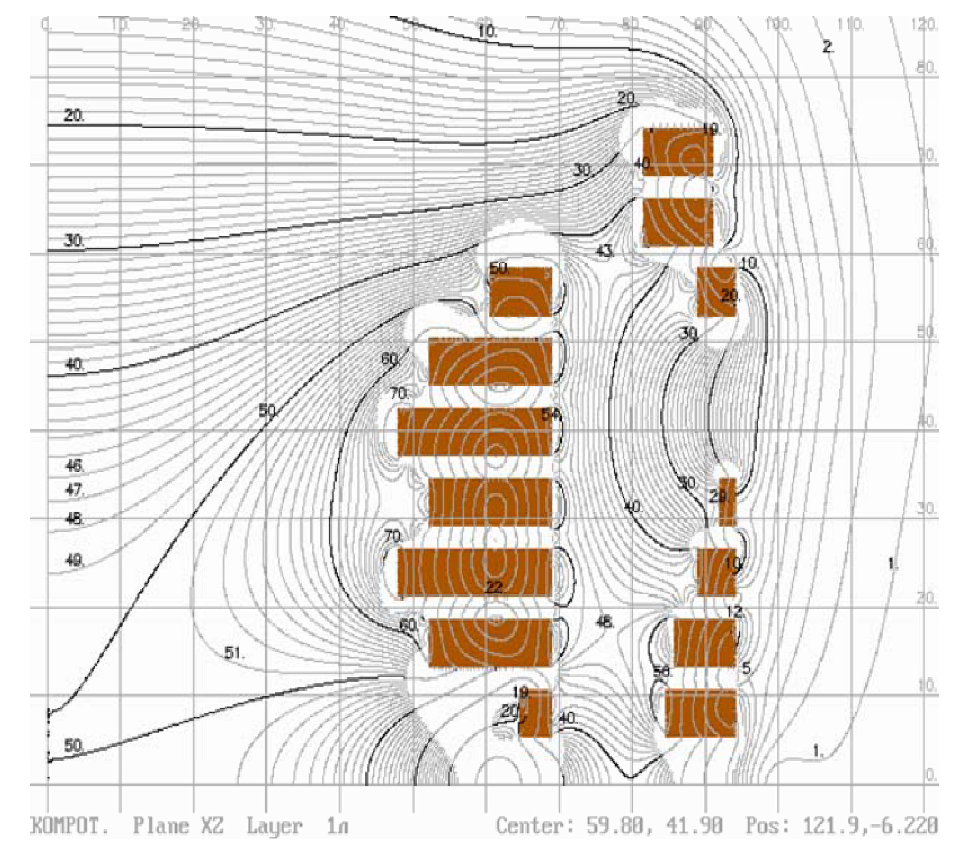
\includegraphics[width=0.5\textwidth]{sol_field1.ps}
\includegraphics[width=0.5\textwidth]{sol_field2.ps}
\caption{\small{(Top) One ``quadrant'' of the 5-T superconducting solenoid 
coil system.  Shown is the inner main coil and the outer compensation coil.  
Also shown are lines of constant field.  (Bottom) The large distance field 
distribution, showing the effect of the compensation coil.  At a 1.5~m radial 
distance at $z$=0 from the symmetry axis, the field strength is below 15~G. 
(Coordinates given in cm.)}}
\label{magnet3}
\end{figure}
%%%%%%%%%%%%%%%%%%%%%%%%%%%%%%%%%%%%%%%%%%%%%%%%%%%%%%%%%%%%%%%%%%%%%%

The total $\int B dl$ on the magnetic axis is 6.0~Tm and the stored energy at 
the 5~T central field is 25~MJ.  The main parameters are given in the 
Table~\ref{mag_parms2}.

%%%%%%%%%%%%%%%%%%%%%%%%%%%%%%%%%%%%%%%%%%%%%%%%%%%%%%%%%%%%%%%%%%%%%%%%%%%%%%
\begin{table}[htbp]
\begin{center}
\begin{tabular} {||l|c||} \hline \hline
\multicolumn{2} {||l||} {Main winding} \\ \hline
Inner diameter      & 943 mm \\ \hline
Aperture            & 780 mm \\ \hline
Max. outer diameter & 1300 mm \\ \hline
Length              & 1225.6 mm \\ \hline
Number of turns     & 4000 \\ \hline \hline
\multicolumn{2} {||l||} {Shielding winding} \\ \hline
Min. inner diameter & 1636 mm \\ \hline
Outer diameter      & 1804 mm \\ \hline
Length              & 1685.2 mm \\ \hline
Number of turns     & 1800 \\ \hline \hline
\multicolumn{2} {||l||} {General} \\ \hline
Inhomogeneity in working area & 5 ppm \\ \hline
Field in center               & 4.5 -- 5.0 T \\ \hline
Field at PMTs                 & $<$18 G \\ \hline
Max. field at the winding     & 6.8 -- 7.5 T \\ \hline
Nominal operating current     & 2399 -- 2665 A \\ \hline
Inductance                    & 6.95 H \\ \hline
Stored energy                 & 19.99 -- 24.68 MJ \\ \hline \hline
\end{tabular}
\end{center}
\caption{\small{Parameters of the solenoid reference winding.}}
\label{mag_parms2}
\end{table}
%%%%%%%%%%%%%%%%%%%%%%%%%%%%%%%%%%%%%%%%%%%%%%%%%%%%%%%%%%%%%%%%%%%%%%%%%%%%%%


%%%%%%%%%%%%%%%%%%%%%%%%%%%%%%%%%%%%%%%%%%%%%%%%%%%%%%%%%%%%%%%%%%%%%%%%
\clearpage
\pagebreak

\chapter{Tracking Systems -- Drift Chambers \& Vertex Tracker}

\fancypagestyle{myheading}{%                % Redefining plain style
\fancyhf{} % clear all header and footer fields
\fancyhead[C]{\vspace{0.5cm}\line(1,0){500}\vspace{-0.5cm}}
\fancyhead[l]{\mbox{\bfseries CLAS12 Technical Design Report}}
\fancyhead[r]{\mbox{\bfseries Version 5.1  \date{\today}}}
\fancyfoot[C]{\mbox{\bfseries  \thepage }}
\fancyfoot[r]{\mbox{\bfseries Tracking Systems}}
\fancyfoot[l]{\vspace{-1cm}\line(1,0){500}}
}
\renewcommand{\headrulewidth}{0pt}
\renewcommand{\footrulewidth}{0pt}
\pagestyle{myheading}

\section{Physics Requirements for {\tt CLAS12} Tracking}

The {\tt CLAS} detector in Hall B is being upgraded to take advantage of 
the increase of the CEBAF beam energy from 6 to 12~GeV, thus the new name,  
{\tt CLAS12}.  There are several broad areas of physics enquiry that drive 
these changes: spectroscopic studies of excited baryons, investigations of 
the influence of nuclear matter on propagating quarks, studies of polarized 
and unpolarized quark distributions, and a comprehensive measurement of 
generalized parton distributions (GPDs).  Many of the reactions of interest 
are electroproduction of exclusive and semi-inclusive final states.  The 
cross sections for these processes are small, necessitating high-luminosity 
experiments.  A variety of simulated experiments rely on luminosities of 
10$^{35}$~cm$^{-2}$s$^{-1}$ to achieve the desired statistical accuracy in 
runs of a few months duration.  The new kinematic range to be explored is 
characterized not only by smaller cross sections, but also by more outgoing 
particles per event, with those particles being emitted with higher values 
of momentum and at smaller laboratory angles.  These basic physics criteria 
drive the design. 

The deep exclusive reactions, in which an electron scattering at moderate to 
high values of $Q^2$ results in a meson-baryon final state, provide the most 
stringent requirements for the {\tt CLAS12} tracking system.  A final state 
of a few high-momentum, forward-going particles (the electron as well as one 
or more mesons), combined with a moderate-momentum baryon emitted at large 
angles, is the typical event type that determines the specifications of the 
tracking system.

The higher momentum and more forward angles of most hadrons leads us to 
split the design into a ``forward'' detector, which covers lab angles between 
5$^\circ$ and 40$^\circ$, and a ``central'' detector for hadrons with angles 
greater than 35$^\circ$.  The higher luminosity goal necessitates the use of 
a solenoidal magnet to shield the detector from M{\o}ller electrons.  To 
reduce interactions between this solenoidal field and the main {\tt CLAS12} 
toroidal field, and to facilitate construction and installation of new 
detector elements, the torus has been re-designed.  It is more compact than 
the present {\tt CLAS} torus, while providing equivalent bending power.  This 
smaller torus design provides several advantages in the overall detector 
design: it decouples the design of the central solenoid and detector from 
that of the torus and forward tracking system, and it makes detector 
installation and removal easier.  

In broad strokes, the detector must provide tracking for laboratory angles as 
small as 5$^\circ$ and as large as 125$^\circ$ in order to cover as much of 
the hadronic center-of-mass region as possible.  We require very good momentum 
and angular resolution for the scattered electron in order to determine the 
virtual photon flux factor, $\Gamma_v$, to an accuracy of a few percent.
Because the average particle momenta will be higher, the resolution of the 
tracking system must be better than the current {\tt CLAS} values; the goal 
for the fractional momentum resolution is 0.5\% to 1\% at a track momentum 
of 5~GeV.  Angular resolutions of about 1~mrad are required for the electron 
in order to know the virtual photon flux factor, and hence, the cross section, 
to a few percent. Finally, good vertex resolution will allow detection of 
secondary decay vertices and serve as a good marker for strangeness production.

Because only about 20\% of the total charged particle momenta is carried by 
tracks in the central region, the fractional momentum resolution requirement
for the central tracking system at a momentum of 1~GeV is 5\% in order to 
match the absolute momentum resolution of the forward tracking system.  This 
momentum resolution of about 50~MeV is necessary in order to positively 
identify a missing pion in these exclusive reactions.  Similarly, to keep our 
knowledge of the individual vector components of the momentum at the 25~MeV 
level, the central trackers angular resolution should be of the order of 
1.5$^\circ$.  Our present design has an expected performance about a factor 
of two better than these simple limits.  

A tracking system capable of achieving these standards was described in the 
PCDR~\cite{pcdr} and quantitatively parameterized in a ``fast'' Monte Carlo 
program~\cite{fastmc}.  A number of {\tt CLAS} collaborators used the model 
of the detector as described in FASTMC in proposals presented at JLab 
PAC30 and PAC32~\cite{PAC30,PAC32}.

%%%%%%%%%%%%%%%%%%%%%%%%%%%%%%%%%%%%%%%%%%%%%%%%%%%%%%%%%%%%%%%%%%%%%%%
\begin{figure}[ht]
\centering
\includegraphics[width=0.60\textwidth]{clas12_system}
\caption{\small{A three-dimensional view of the proposed {\tt CLAS12} 
detector highlighting the various subsystems.}}
\label{clas12}
\end{figure}
%%%%%%%%%%%%%%%%%%%%%%%%%%%%%%%%%%%%%%%%%%%%%%%%%%%%%%%%%%%%%%%%%%%%%%%

\section{Tracking System Design}

As noted above, the {\tt CLAS12} detector is divided into a forward and a 
central detector.  Fig~\ref{clas12} shows a perspective view of the 
{\tt CLAS12} detector.  A solenoid magnet surrounds the target,  followed 
by a M{\o}ller absorber on the beam-line and a high-threshold {\v C}erenkov 
counter for electron identification.  Besides curling background M{\o}ller 
electrons into the absorber, the solenoid provides a nearly constant magnetic 
field that allows charged particle momentum determination by a set of 
``central tracking chambers'' consisting of 8 layers of silicon strip sensors.
This central tracking region covers polar angles from 35$^\circ$ to 
125$^\circ$.  Just downstream of the cylindrical central tracker are the 
``forward vertex chambers'': 6 layers of silicon strip chambers.  Downstream 
of the high-threshold {\v C}erenkov counter is the torus magnet that supports 
three ``regions'' of ``forward drift chambers'', designated as Regions~1, 2, 
and 3.  Surrounding and downstream of the torus/drift chamber assembly are 
the forward time-of-flight counters, a low-threshold {\v C}erenkov counter 
for hadron identification, and two sets of electromagnetic shower counters.  
This document describes each of the elements of the {\tt CLAS12} tracking 
system, the central tracker, the forward vertex tracker, and the forward 
drift chambers.

We have designed the tracking detectors with these external constraints: a 
solenoid of 5~T central field value and a radius available for tracking 
detectors of 25~cm, a new torus with a different aspect ratio but with the 
same number of amp-turns as the present {\tt CLAS} torus, an expected
background rate consistent with a luminosity of 10$^{35}$~cm$^{-2}$s$^{-1}$, 
and a separation between the ``forward'' and ``central'' regions defined to 
be at about 40$^\circ$; specifically the forward tracking chambers are 
designed to cover scattering angles between 5$^\circ$ and 40$^\circ$ and the 
central tracker will cover 35$^\circ$ to 125$^\circ$.  Although the torus 
cryostat will limit the azimuthal coverage to about 50\% at 5$^\circ$, our 
goal is that the inactive portion of the drift chambers not further intrude 
into the active volume; i.e. the dead areas of the drift chambers (endplates, 
electronics, etc.) will be located in the ``shadow'' of the coil as viewed 
from the target.  For Region~2, this is not possible; but we shall try to 
minimize this dead area.  To summarize, we are designing the {\tt CLAS12} 
tracking system with the requirements shown in Table~\ref{tracker-specs}.

%%%%%%%%%%%%%%%%%%%%%%%%%%%%%%%%%%%%%%%%%%%%%%%%%%%%%%%%%%%%%%%%%%%%%%%%%
\begin{table}[htbp]
\begin{center}
\begin{tabular} {||l|c|c||} \hline \hline
                    & {\bf Fwd. Tracker }    & {\bf Central Tracker} \\ \hline
Angular coverage    & 5$^\circ$ - 40$^\circ$ & 35$^\circ$ - 125$^\circ$  \\ \hline
Momentum resolution & $dp/p < 1$$\%$         & $dp/p < 5$$\%$            \\ \hline
$\theta$ resolution & 1~mrad                 & 1~mrad                    \\ \hline
$\theta$ resolution & 1~mrad                 & 5 - 10~mrad               \\ \hline
$\phi$ resolution   & 1~mrad/$\sin \theta$   & 5~mrad/$\sin \theta$      \\ \hline
Luminosity          & 10$^{35}$~cm$^{-2}$s$^{-1}$ & 10$^{35}$~cm$^{-2}$s$^{-1}$ \\ \hline \hline
\end{tabular}
\caption{\small{General specifications for {\tt CLAS12} tracking.}}
\label{tracker-specs}
\end{center}
\end{table}
%%%%%%%%%%%%%%%%%%%%%%%%%%%%%%%%%%%%%%%%%%%%%%%%%%%%%%%%%%%%%%%%%%%%%%%%%

\subsection{Forward Tracking Design}

The higher beam energies available to {\tt CLAS12} mean that tracks will go 
more forward and have higher momenta than for the present {\tt CLAS} 
experiments.  We thus require better resolution from the forward drift 
chambers.  Our design should give better spatial resolution than the present 
{\tt CLAS} chambers for several reasons: the use of thicker (30-$\mu$m 
diameter) sense wires will result in a more linear drift velocity, all cells 
in a superlayer will be identical, easing the calibration, and the simpler 
mechanical structure should make these chambers easier to survey.  The other 
feature of higher energy and associated smaller cross sections, requires the 
use of higher intensity beams.  The resultant higher backgrounds represent 
the primary motivation for the central solenoidal magnet and M{\o}ller 
absorber.  The higher background can also be mitigated by cells that cover a 
smaller angular range and have a smaller active time window.

Forward tracks (angles between 5$^\circ$ and 40$^\circ$) will be 
momentum-analyzed by passing through the magnetic field of the torus.  The 
magnet provides an integral $Bdl$ of almost 3 T-m at 10$^\circ$, falling
to about 1 T-m at 30$^\circ$ (see Fig.~\ref{bdl}).

%%%%%%%%%%%%%%%%%%%%%%%%%%%%%%%%%%%%%%%%%%%%%%%%%%%%%%%%%%%%%%%%%%%%%%%%%%%
\begin{figure}[htbp]
\vspace{6.8cm}
\special{psfile=btoro1.ps hscale=55 vscale=40 hoffset=90 voffset=-10}
\caption{\small{The integral of the $B$ field times path length along rays 
from the target at various angles.}}
\label{bdl}
\end{figure}
%%%%%%%%%%%%%%%%%%%%%%%%%%%%%%%%%%%%%%%%%%%%%%%%%%%%%%%%%%%%%%%%%%%%%%%%%%%

Such forward tracks will first pass through six layers of the forward silicon 
vertex tracker (FST); a silicon strip tracker with a strip pitch of 
150~$\mu$m arranged with alternating $V$-$W$ stereo layers with a stereo angle 
of $\pm$12$^\circ$, located about 27~cm from the target.  These tracks will 
then traverse the high-threshold {\v C}erenkov counter (HTCC) before 
entering the Region~1 drift chamber at a distance of 2.1~m from the target.  
The track continues through the magnetic field region and its trajectory is 
measured in two more drift chambers, denoted Regions~2 and 3, respectively.  
The Region~2 and 3 chambers are located at 3.3 and 4.5~m from the target,
respectively.  The FST should localize hits with an estimated accuracy of 
about 50~$\mu$m perpendicular to the strip direction, while the three regions 
of drift chambers are expected to have spatial resolutions of about
250~$\mu$m per layer.  The expected momentum resolution from such an assembly 
is a function of angle, ranging from about 0.3\% at 5$^\circ$ to about 1.0\% 
at 30$^\circ$, and nearly constant as a function of momentum.  The angular 
resolution falls rapidly with increasing momentum, but should be better than 
2~mrad at a momentum of 1~GeV.

\subsection{Central Tracking Design}

The momentum and angular resolution goals for the central tracker are set by 
the requirement that we be able to positively identify a single missing pion; 
roughly a 50~MeV momentum resolution is needed, i.e. a fractional momentum 
resolution of 5\% or better at a track momentum of 1~GeV.  Our design consists 
of 8 layers of silicon strips with alternating plus and minus stereo angle 
strips.  Each detector plane is formed as a polygonal shell with the silicon
strips running along the $z$-direction.  Each single-sided layer is comprised 
of 300-$\mu$m thick silicon.  This detector has good intrinsic resolution in 
the $r$-$\phi$ coordinate due to the small strip pitch (150~$\mu$m readout and 
75~$\mu$m implant pitch). It relies on a small stereo angle to determine the 
$r$-$z$ position of tracks.  

A solenoidal magnet contains the target, the silicon vertex tracker, the 
central time-of-flight system (CTOF), and the M{\o}ller absorber.  Charged 
particles with emission angles greater than 35$^\circ$ follow helical paths 
through the 8 layers of the BST, which are arranged into four $V$-$W$ modules 
with ``$V$'' and ``$W$'' referring to strip orientations.  The time resolution 
of the CTOF ($\sim$60~ps) will enable particle identification of the charged 
tracks, as well as allowing for a very efficient rejection of out-of-time 
accidentals.

\section{Silicon Vertex Tracker for {\tt CLAS12}}

\subsection{Overview}

The Silicon Vertex Tracker (SVT), anticipated to have $\sim$65,000 channels, 
will consist of a forward silicon tracker (FST) and a barrel silicon tracker 
(BST).  The $\theta$-coverage  of the forward part is from 5$^\circ$ to 
35$^\circ$ and that of the barrel part is from 35$^\circ$ to 125$^\circ$.  
Conceptual design studies started in 2004~\cite{CN2004-42}.  For both the 
forward and barrel parts, the $\phi$ coverage is nearly $2\pi$.  The SVT will 
be centered inside the 1800-mm long solenoid, that has an outer and inner 
diameter of 2040~mm and 780~mm, respectively
.
%%%%%%%%%%%%%%%%%%%%%%%%%%%%%%%%%%%%%%%%%%%%%%%%%%%%%%%%%%%%%%%%%%%%%%%
\begin{figure}[htbp]
\centering
\includegraphics[width=0.65\textwidth]{solenoid}
\caption{\small{Side view of the solenoid magnet (units in inches -- with mm 
in parentheses).}}
\label{fig:solenoid}
\end{figure}
%%%%%%%%%%%%%%%%%%%%%%%%%%%%%%%%%%%%%%%%%%%%%%%%%%%%%%%%%%%%%%%%%%%%%%%

\subsection{Configuration}

Several configurations of the BST and the FST were studied~\cite{CN2006-21} 
with the aim to optimize the layout with respect to operability, performance 
and cost.  The BST is designed to have four regions and the FST is designed 
to have three regions.  The BST and FST form two independent detectors (see
Fig.~\ref{side-svt-layout}), providing operational flexibility in that either 
or both detectors could be used in a given experiment. There are only three 
FST regions because the FST will be used in conjunction with the three drift 
chambers in the forward region.   

%%%%%%%%%%%%%%%%%%%%%%%%%%%%%%%%%%%%%%%%%%%%%%%%%%%%%%%%%%%%%%%%%%%%%%%
\begin{figure}[htbp]
\centering
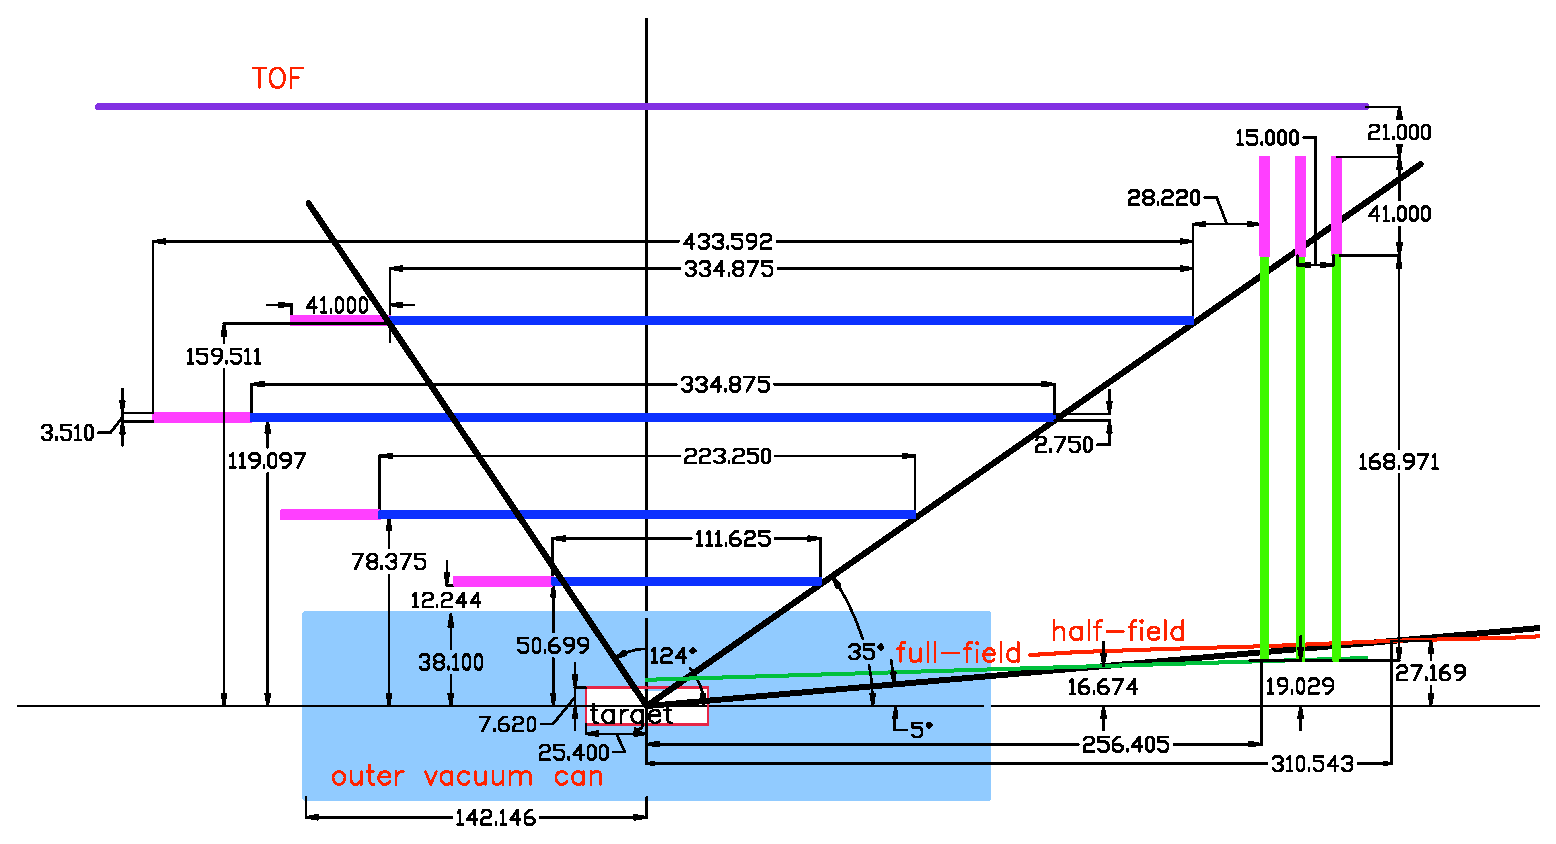
\includegraphics[width=0.9\textwidth]{side-view2a}
\caption{\small{Side view of the SVT showing the layout of the barrel and 
forward regions (all dimensions in mm).}}
\label{side-svt-layout}
\end{figure}
%%%%%%%%%%%%%%%%%%%%%%%%%%%%%%%%%%%%%%%%%%%%%%%%%%%%%%%%%%%%%%%%%%%%%%%

%%%%%%%%%%%%%%%%%%%%%%%%%%%%%%%%%%%%%%%%%%%%%%%%%%%%%%%%%%%%%%%%%%%%%%%
\begin{figure}[htbp]
\centering
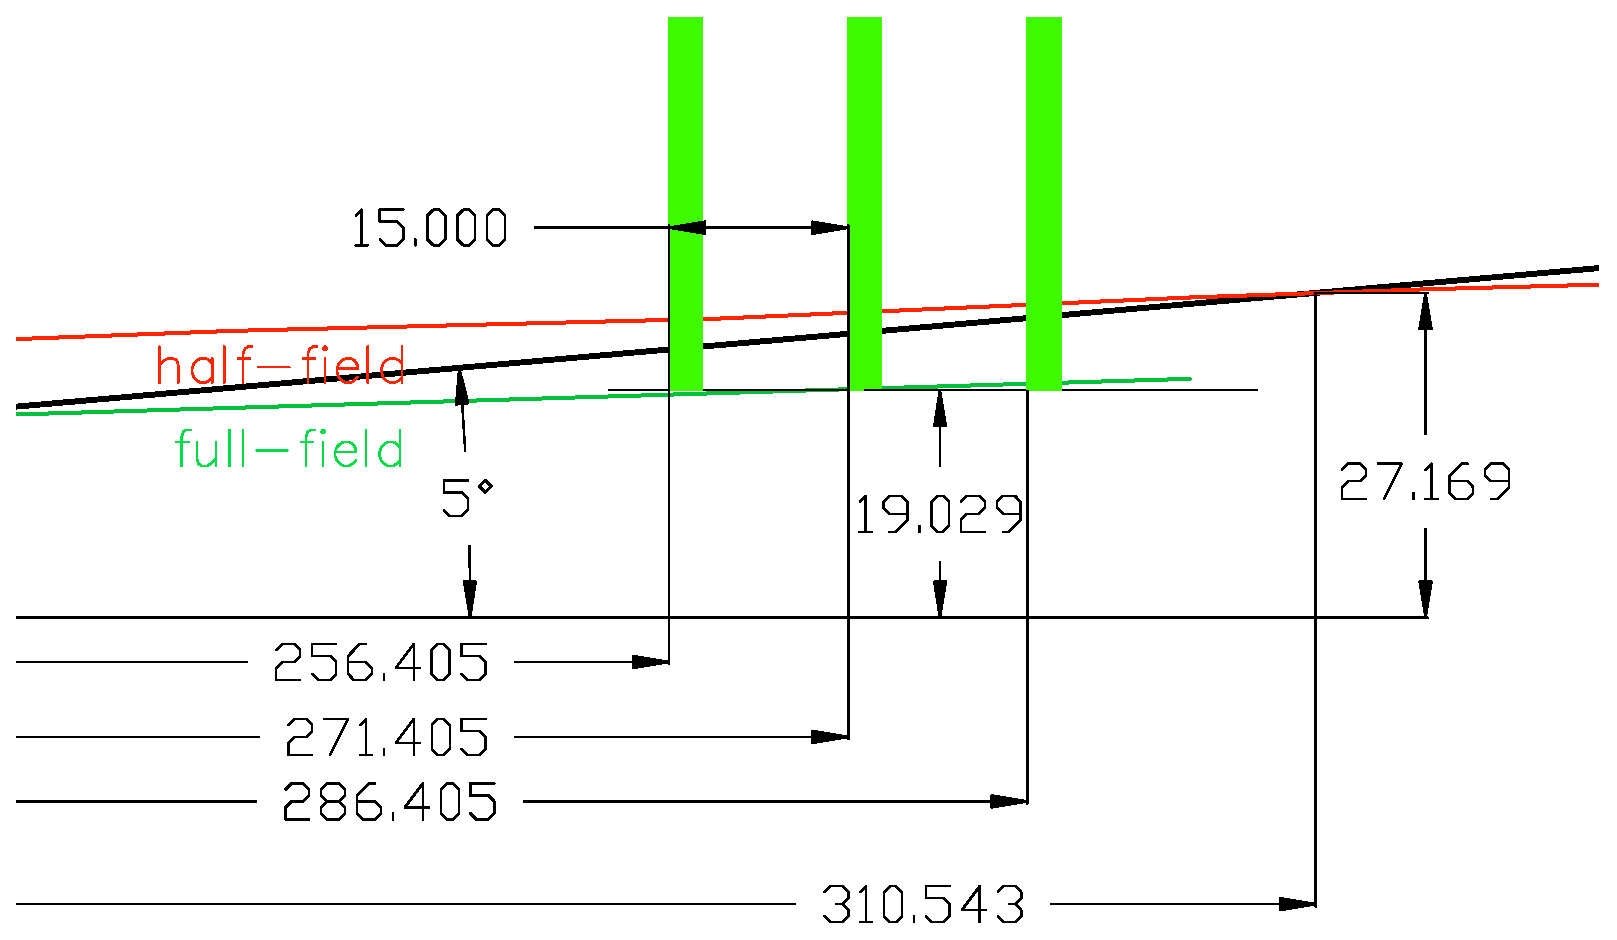
\includegraphics[width=0.9\textwidth]{cone_beam}
\caption{\small{Close up view of the three forward SVT regions near the beam 
line and the M{\o}ller absorber.}}
\label{cone_beam}
\end{figure}
%%%%%%%%%%%%%%%%%%%%%%%%%%%%%%%%%%%%%%%%%%%%%%%%%%%%%%%%%%%%%%%%%%%%%%%

\subsection{Rate Estimates}

Event and background rates were estimated using a GEANT simulation
\cite{CN2004-13,CN2006-20}.  These studies indicate that the maximum rate, 
including electromagnetic background for a full-field setting of the solenoid 
(5~T) is $\sim$40~MHz in the FST and $\sim$60~MHz in the BST.  In 
Fig.~\ref{side-svt-layout}, the green and red curve (full and half-field 
settings of the solenoid) along the beam axis is the M{\o}ller electron 
envelope, on the surface of which the rate is $\sim$1~MHz. The rate drops 
rapidly with increasing scattering angle~\cite{CN2006-20}.

To keep M{\o}ller electron rates on the FST sensors less than 1~MHz, the first 
region of the FST is placed at $z$=256.405~mm (see Figs.~\ref{side-svt-layout} 
and \ref{cone_beam}), past the intersection of the M{\o}ller electron envelope 
for the full-field setting with the keep-out zone, defined to be a cone with 
a half opening angle of 5$^\circ$.  The second and third regions of the FST 
are at $z$=271.405~mm and $z$=286.405~mm, respectively.

\subsection{Forward Silicon Tracker (FST)}

The trapezoidal sensors of the FST are designed to be identical.  Such a 
design requires that the regions be parallel to the beam axis, rather than 
ride the 5$^\circ$ keep-out cone.  In $\phi$, each FST region consists of 15 
sectors as shown in Fig.~\ref{fig:front-cone}.  

%%%%%%%%%%%%%%%%%%%%%%%%%%%%%%%%%%%%%%%%%%%%%%%%%%%%%%%%%%%%%%%%%%%%%%%
\begin{figure}[htbp]
\centering
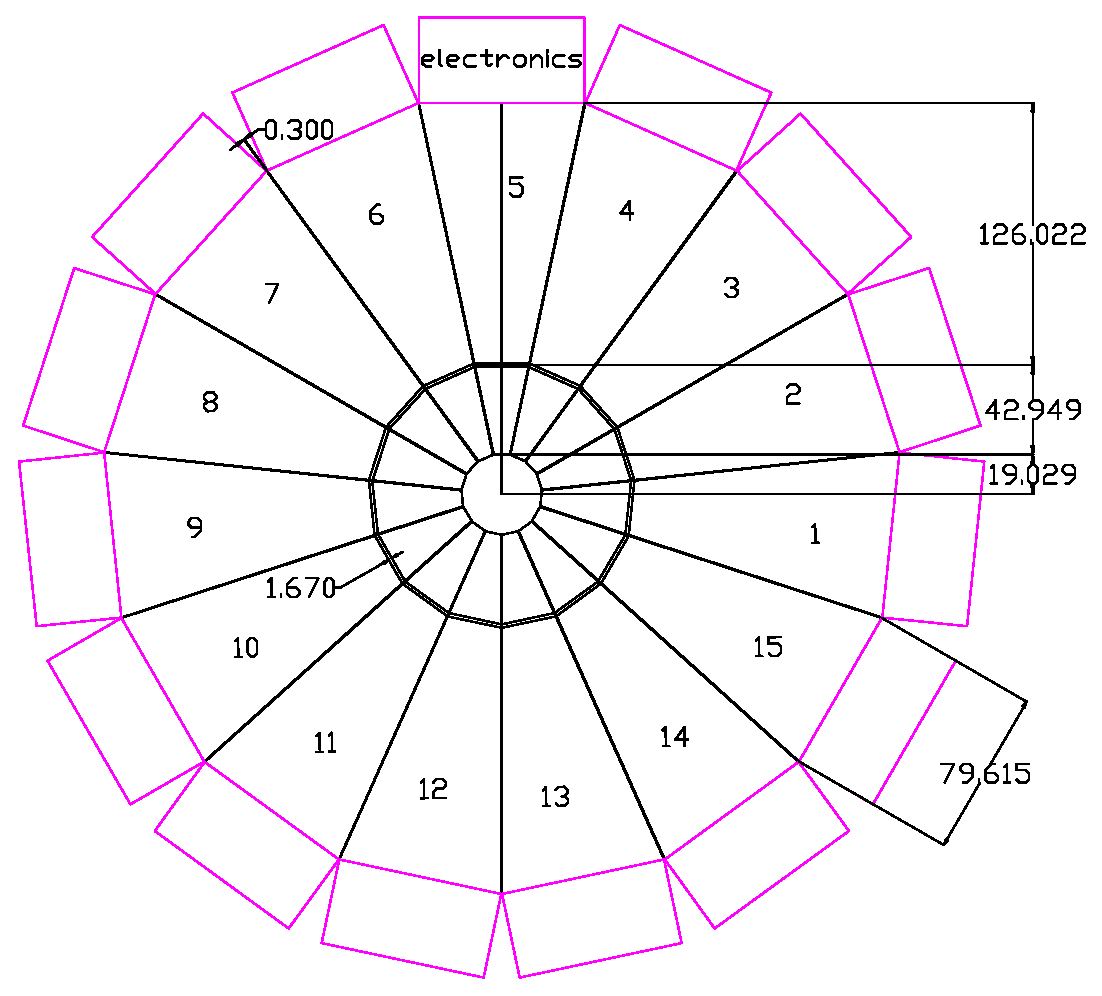
\includegraphics[width=0.5\textwidth]{front-cone}
\caption{\small{Front view of the first region of the FST showing the
layout and positioning of the trapezoidal sensors.}}
\label{fig:front-cone}
\end{figure}
%%%%%%%%%%%%%%%%%%%%%%%%%%%%%%%%%%%%%%%%%%%%%%%%%%%%%%%%%%%%%%%%%%%%%%%

In the critical region around the beam axis at $r\sim$19~mm, because the 
sensors are trapezoidal, the $V$ and the $W$ layers of a region each have 
$\sim$40 strips per sector, distributed over 2$\pi$, a total of $\sim$600 
strips per layer.  The rate near the beam axis has to be handled by these 
600 strips.  Though 600 strips per layer around the beam axis appears to be 
a small number, the readout electronics associated with these strips will 
on average have a rate-load of $\sim$10~kHz that can be handled by the 
readout electronics.

%%%%%%%%%%%%%%%%%%%%%%%%%%%%%%%%%%%%%%%%%%%%%%%%%%%%%%%%%%%%%%%%%%%%%%%
\begin{figure}[htbp]
\centering
\includegraphics[width=0.8\textwidth]{rear-barrel}
\caption{\small{Rear view of the barrel section of the SVT showing the
sensor partitioning in each region.}}
\label{fig:rear-barrel}
\end{figure}
%%%%%%%%%%%%%%%%%%%%%%%%%%%%%%%%%%%%%%%%%%%%%%%%%%%%%%%%%%%%%%%%%%%%%%%

\subsection{Barrel Silicon Tracker (BST)}

The four BST regions have $\sim$240~mm of radial space available for tracking.
Having four regions instead of the minimum three needed for track 
reconstruction provides a redundant tracking region that mitigates the risk of 
tracking inefficiencies due to layer problems such as malfunctioning strips, 
electronics, or noise.  Further, tracking simulations indicate that with four 
regions instead of three, the probability of reconstructing fake tracks for a 
given number of correlated background hits per region (that are randomly 
distributed over the four BST regions) is reduced by a factor of three.  Our 
simulations indicate that four regions should be able to handle about forty 
background hits in the time window.  The first BST region has a diameter of 
$\sim$101~mm.  The second, third, and fourth BST regions have diameters of 
$\sim$157~mm, $\sim$239~mm, and $\sim$320~mm, respectively.  The radial 
distance, $\Delta r$, between region four and region one of the BST has been 
chosen to maximize momentum resolution, which has an inverse square dependence 
on $\Delta r$.  In $\phi$, the BST regions, from the innermost to the 
outermost, are partitioned in 8, 12, 18, and 24 sectors, as shown in 
Fig.~\ref{fig:rear-barrel}.  Studies indicate that track loss due to the 
cracks between adjacent sectors in the BST is less than 5\% for a half-field 
setting of the solenoid, as long as the cracks are no wider than 2~mm.

\subsection{Dicing Layout}

The dicing layout for a trapezoidal sensor from a 6-in diameter wafer is 
shown in Fig.~\ref{fig:trap-dicing}.  The dicing process demands a 
keep-out zone of 0.25~in around the edge of the wafer.

%%%%%%%%%%%%%%%%%%%%%%%%%%%%%%%%%%%%%%%%%%%%%%%%%%%%%%%%%%%%%%%%%%%%%%%
\begin{figure}[htbp]
\centering
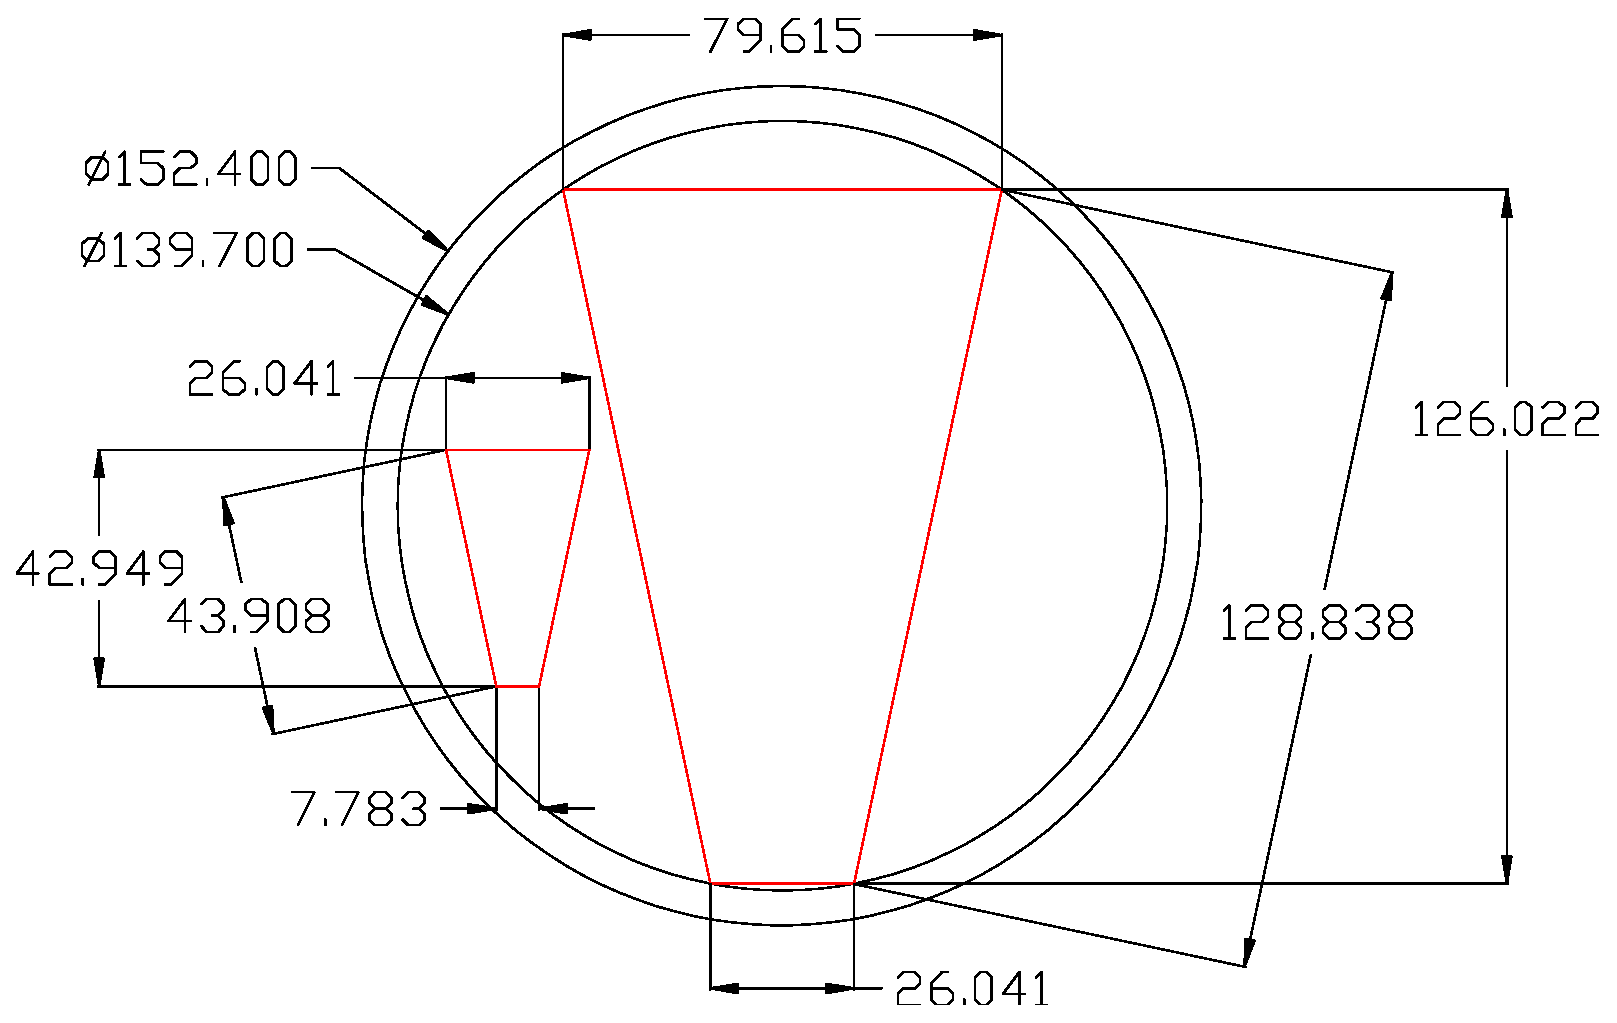
\includegraphics[width=0.6\textwidth]{trap-dicing}
\caption{\small{Trapezoidal sensor dicing from a standard 6-in wafer. All 
units in mm.}}
\label{fig:trap-dicing}
\end{figure}
%%%%%%%%%%%%%%%%%%%%%%%%%%%%%%%%%%%%%%%%%%%%%%%%%%%%%%%%%%%%%%%%%%%%%%%


The BST dicing layout of a 6-in wafer, as shown in 
Fig.~\ref{fig:barrel-dicing}, is such that it provides the longest sensors 
possible.  Such a layout reduces the number of sensors needed for the BST 
modules.  Further, cost is reduced by maximizing the yield of sensors from a 
single wafer -- minimizing the total number of wafers required for the BST.  
All BST regions use sensors with a cut size of 111.62~mm $\times$ 42.00~mm 
$\times$ 0.300~mm.

%%%%%%%%%%%%%%%%%%%%%%%%%%%%%%%%%%%%%%%%%%%%%%%%%%%%%%%%%%%%%%%%%%%%%%%
\begin{figure}[htbp]
\centering
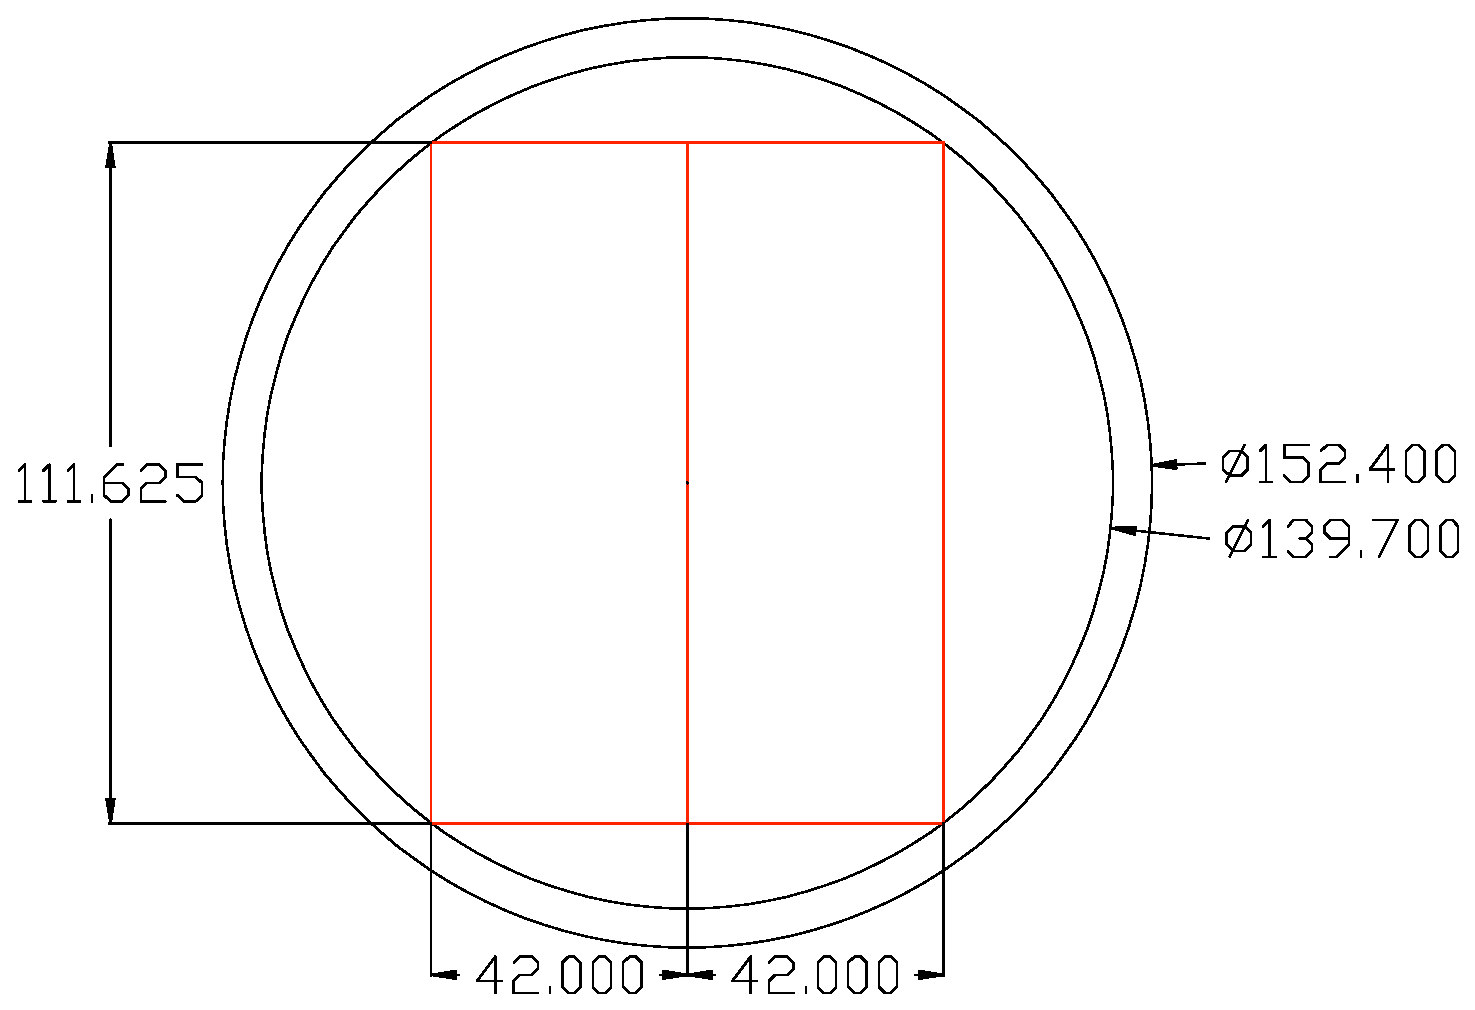
\includegraphics[width=0.6\textwidth]{barrel-dicing}
\caption{\small{Barrel sensor dicing from a standard 6-in wafer. All units 
in mm.}}
\label{fig:barrel-dicing}
\end{figure}
%%%%%%%%%%%%%%%%%%%%%%%%%%%%%%%%%%%%%%%%%%%%%%%%%%%%%%%%%%%%%%%%%%%%%%%

\subsection{Module and Strip Layout}

Fig.~\ref{fig:sensor-detail} shows the cross sectional view of the sensor.  
The lengths of the readout strips of the SVT vary from 0.5~cm to 33~cm.  The 
strip width is $\sim$8~$\mu$m and the implant depth $\sim$1.2~$\mu$m.

%%%%%%%%%%%%%%%%%%%%%%%%%%%%%%%%%%%%%%%%%%%%%%%%%%%%%%%%%%%%%%%%%%%%%%%
\begin{figure}[htbp]
\centering
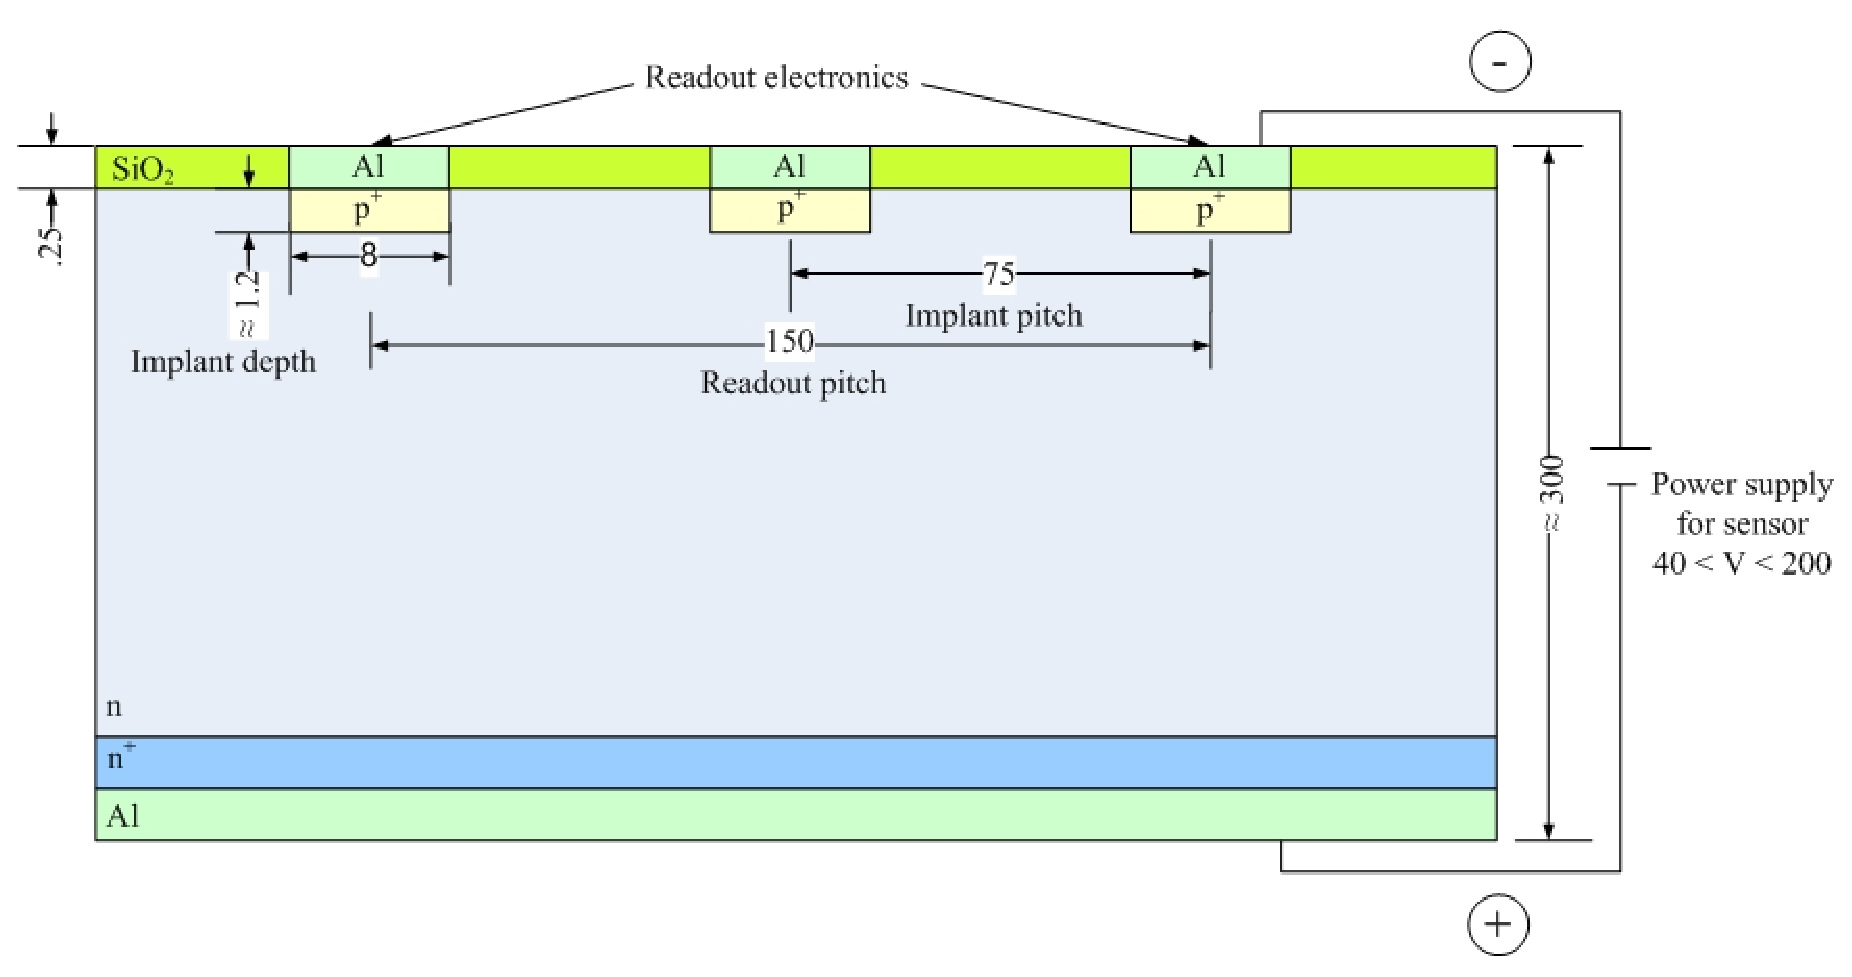
\includegraphics[width=0.7\textwidth]{sensor-detail}
\caption{\small{Cross sectional view of a sensor showing the different
layers and the spacing of the strips (all units in $\mu$m).}}
\label{fig:sensor-detail}
\end{figure}
%%%%%%%%%%%%%%%%%%%%%%%%%%%%%%%%%%%%%%%%%%%%%%%%%%%%%%%%%%%%%%%%%%%%%%%

A completed module in the BST has 256 readout channels per layer -- 512 
channels in all per module.  The modules of the FST have 512 channels per 
layer -- 1024 channels total per module.  Each FST sector consists of a 
module -- a single trapezoidal unit as shown in Fig.~\ref{fig:trap-dicing} 
that consists of a $V$ and a $W$ silicon layer that sandwich a 2-mm-thick 
Rohacell~71 carbon fiber composite.   

To reduce costs, the $V$ and $W$ layers for the modules of the different 
BST regions are made of one or more fundamental rectangular sensors.  If 
more than one sensor is needed for a module, the sensors are wire-bonded 
together.  Modules of the BST Regions 1, 2, 3, and 4 have 1, 2, 3, and 3 
sensors, respectively (see Fig.~\ref{side-svt-layout}).  Fig.~\ref{svt_views}
shows 3D renderings of how the complete SVT system is expected to look.  

%%%%%%%%%%%%%%%%%%%%%%%%%%%%%%%%%%%%%%%%%%%%%%%%%%%%%%%%%%%%%%%%%%%%%%%
\begin{figure}[htbp]
\vspace{6.7cm}
\special{psfile=overall-rear.eps hscale=33 vscale=33 hoffset=0 
voffset=0}
\special{psfile=overall-side.eps hscale=33 vscale=33 hoffset=245 
voffset=0}
\caption{\small{Overall conceptual renderings for the SVT showing a rear
view (left) and a side view (right).}}
\label{svt_views}
\end{figure}
%%%%%%%%%%%%%%%%%%%%%%%%%%%%%%%%%%%%%%%%%%%%%%%%%%%%%%%%%%%%%%%%%%%%%%%

Table~\ref{matprop} gives the radiation length of the materials used for 
the sensor structure.  Because of the large variety of commercial graphite 
fibers available for GFRP (glass fiber reinforced polymer) composites, they 
have an added bonus of being easily obtainable at an acceptable cost.  The 
preferred structural materials are GFRP and Rohacell.  The total anticipated 
radiation length for the BST is $\sim$3.5\% and for the FST $\sim$2.7\%. 

%%%%%%%%%%%%%%%%%%%%%%%%%%%%%%%%%%%%%%%%%%%%%%%%%%%%%%%%%%%%%%%%%%%%%%%
\begin{table}[htbp]
\begin{center}
\begin{tabular}{|c|c|c|c|} \hline
Material & Radiation Length (mm) & Thickness (mm) & Radiation Length [\%X0] 
\\ \hline
Silicon    &   93.7 & 0.300 & 0.320 \\ \hline
Epoxy      &  443.7 & 0.025 & 0.007 \\ \hline
GFRP       &  250.0 & 0.250 & 0.100 \\ \hline
Rohacell71 & 5450.0 & 2.000 & 0.040 \\ \hline
GFRP       &  250.0 & 0.250 & 0.100 \\ \hline
Epoxy      &  443.7 & 0.025 & 0.007 \\ \hline
Silicon    &   93.7 & 0.300 & 0.320 \\ \hline 
\end{tabular}
\end{center}
\caption{\small{Material thickness with radiation lengths for the different
layers that make up the sensors of the BST and FST.}}
\label{matprop}
\end{table}
%%%%%%%%%%%%%%%%%%%%%%%%%%%%%%%%%%%%%%%%%%%%%%%%%%%%%%%%%%%%%%%%%%%%%%%

The readout pitch for the strips, which is twice the implant pitch, is 
determined by the minimization, as far as affordable, of spatial resolution.  
Based on this criterion, the strips are designed to have an implant pitch of 
0.075~mm and a readout pitch of 0.150~mm.  The expected spatial resolution 
for this pitch spacing is about 0.050~mm and the occupancy in a layer of an 
FST region, for half-field operation of the solenoid, is less than $\sim$1.5\%.
The $V$ and $W$ layer strips for the FST sensors run parallel to the edges of 
the trapezoid (see Fig.~\ref{fig:trap-strip}), with the strips intersecting at 
an angle of 12$^\circ$.

For the BST, the 42-mm width of the sensor accommodates 256 input 
channels, at a readout strip pitch of 0.150~mm, to the two SVX4 ASICs, and 
the required keep-out zones around the sensor (see Fig.~\ref{barrel_strip}).  
The $V$ and $W$ strips are designed such that strip 1 is at an 
angle of 0$^\circ$ with respect to the length axis of the rectangular BST 
sensors and strip 256 is at an angle of 3$^\circ$.  This was done to minimize
sensor dead area.  Details are shown in Fig.~\ref{barrel_strip}.  

%%%%%%%%%%%%%%%%%%%%%%%%%%%%%%%%%%%%%%%%%%%%%%%%%%%%%%%%%%%%%%%%%%%%%%%
\begin{figure}[htbp]
\centering
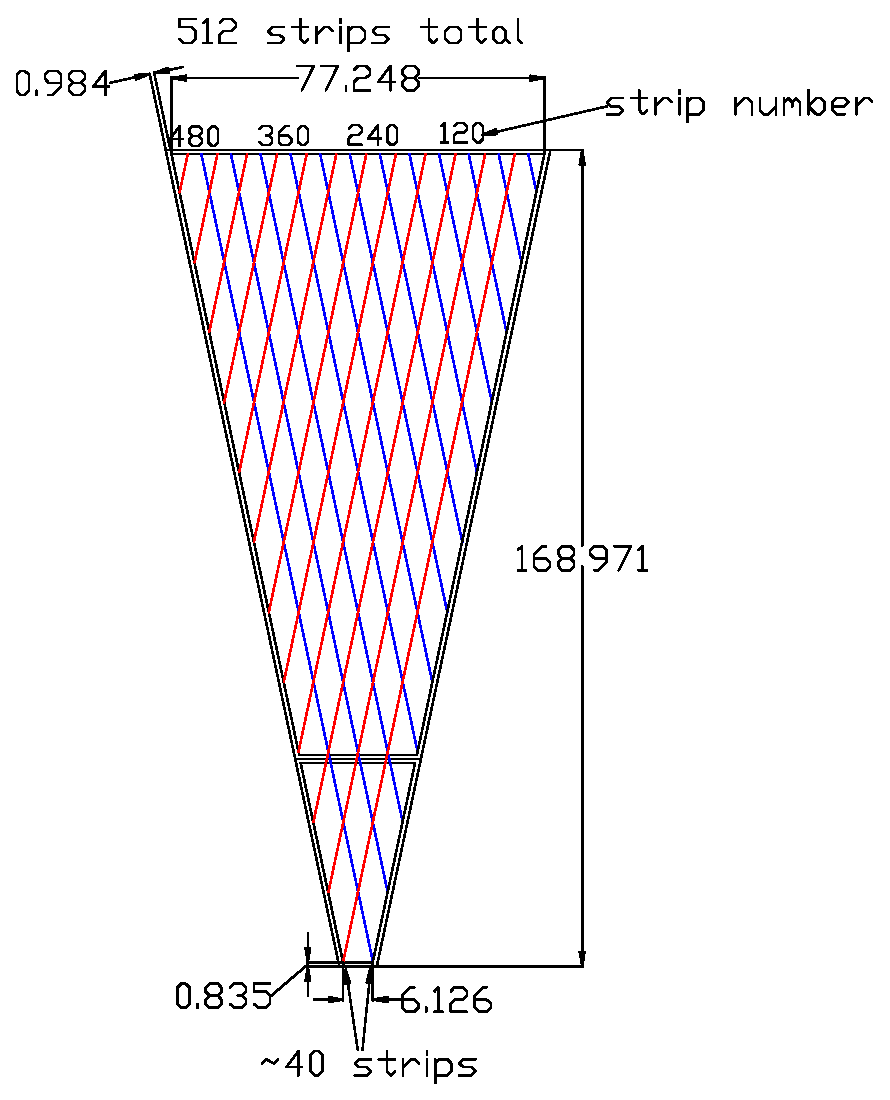
\includegraphics[width=0.6\textwidth]{trap-strip}
\caption{\small{Strip layout for the trapezoidal sensors. All units 
in mm.}}
\label{fig:trap-strip}
\end{figure}
%%%%%%%%%%%%%%%%%%%%%%%%%%%%%%%%%%%%%%%%%%%%%%%%%%%%%%%%%%%%%%%%%%%%%%%

%%%%%%%%%%%%%%%%%%%%%%%%%%%%%%%%%%%%%%%%%%%%%%%%%%%%%%%%%%%%%%%%%%%%%%%
\begin{figure}[htbp]
\centering
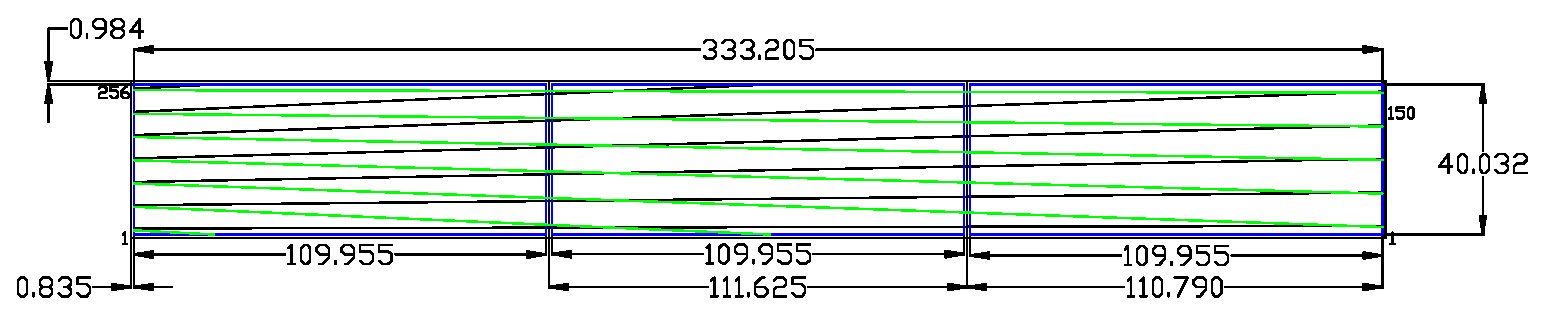
\includegraphics[width=\textwidth]{barrel-strip}
\caption{\small{A standard BST module showing the $V$ and $W$ strips.
All units in mm.}}
\label{barrel_strip}
\end{figure}
%%%%%%%%%%%%%%%%%%%%%%%%%%%%%%%%%%%%%%%%%%%%%%%%%%%%%%%%%%%%%%%%%%%%%%%

\section{Mechanical}

\subsection{Support Structure}

Fig.~\ref{svt_support} shows a view of the complete SVT, including its 
support structure.  A large stainless-steel tube is used to support the BST, 
and the FST is supported off of the BST.   The size and stiffness of the 
support tube seems extreme, but it is a simple system that has been used to 
support other detectors in high magnetic fields in {\tt CLAS} experiments, 
such as the light-weight BONUS detector.   It is expected that the total 
weight of the SVT is less than 10~kg. The calculated deflection of the 
support pipe is 0.033~mm.

%%%%%%%%%%%%%%%%%%%%%%%%%%%%%%%%%%%%%%%%%%%%%%%%%%%%%%%%%%%%%%%%%%%%%%%
\begin{figure}[htbp]
\centering
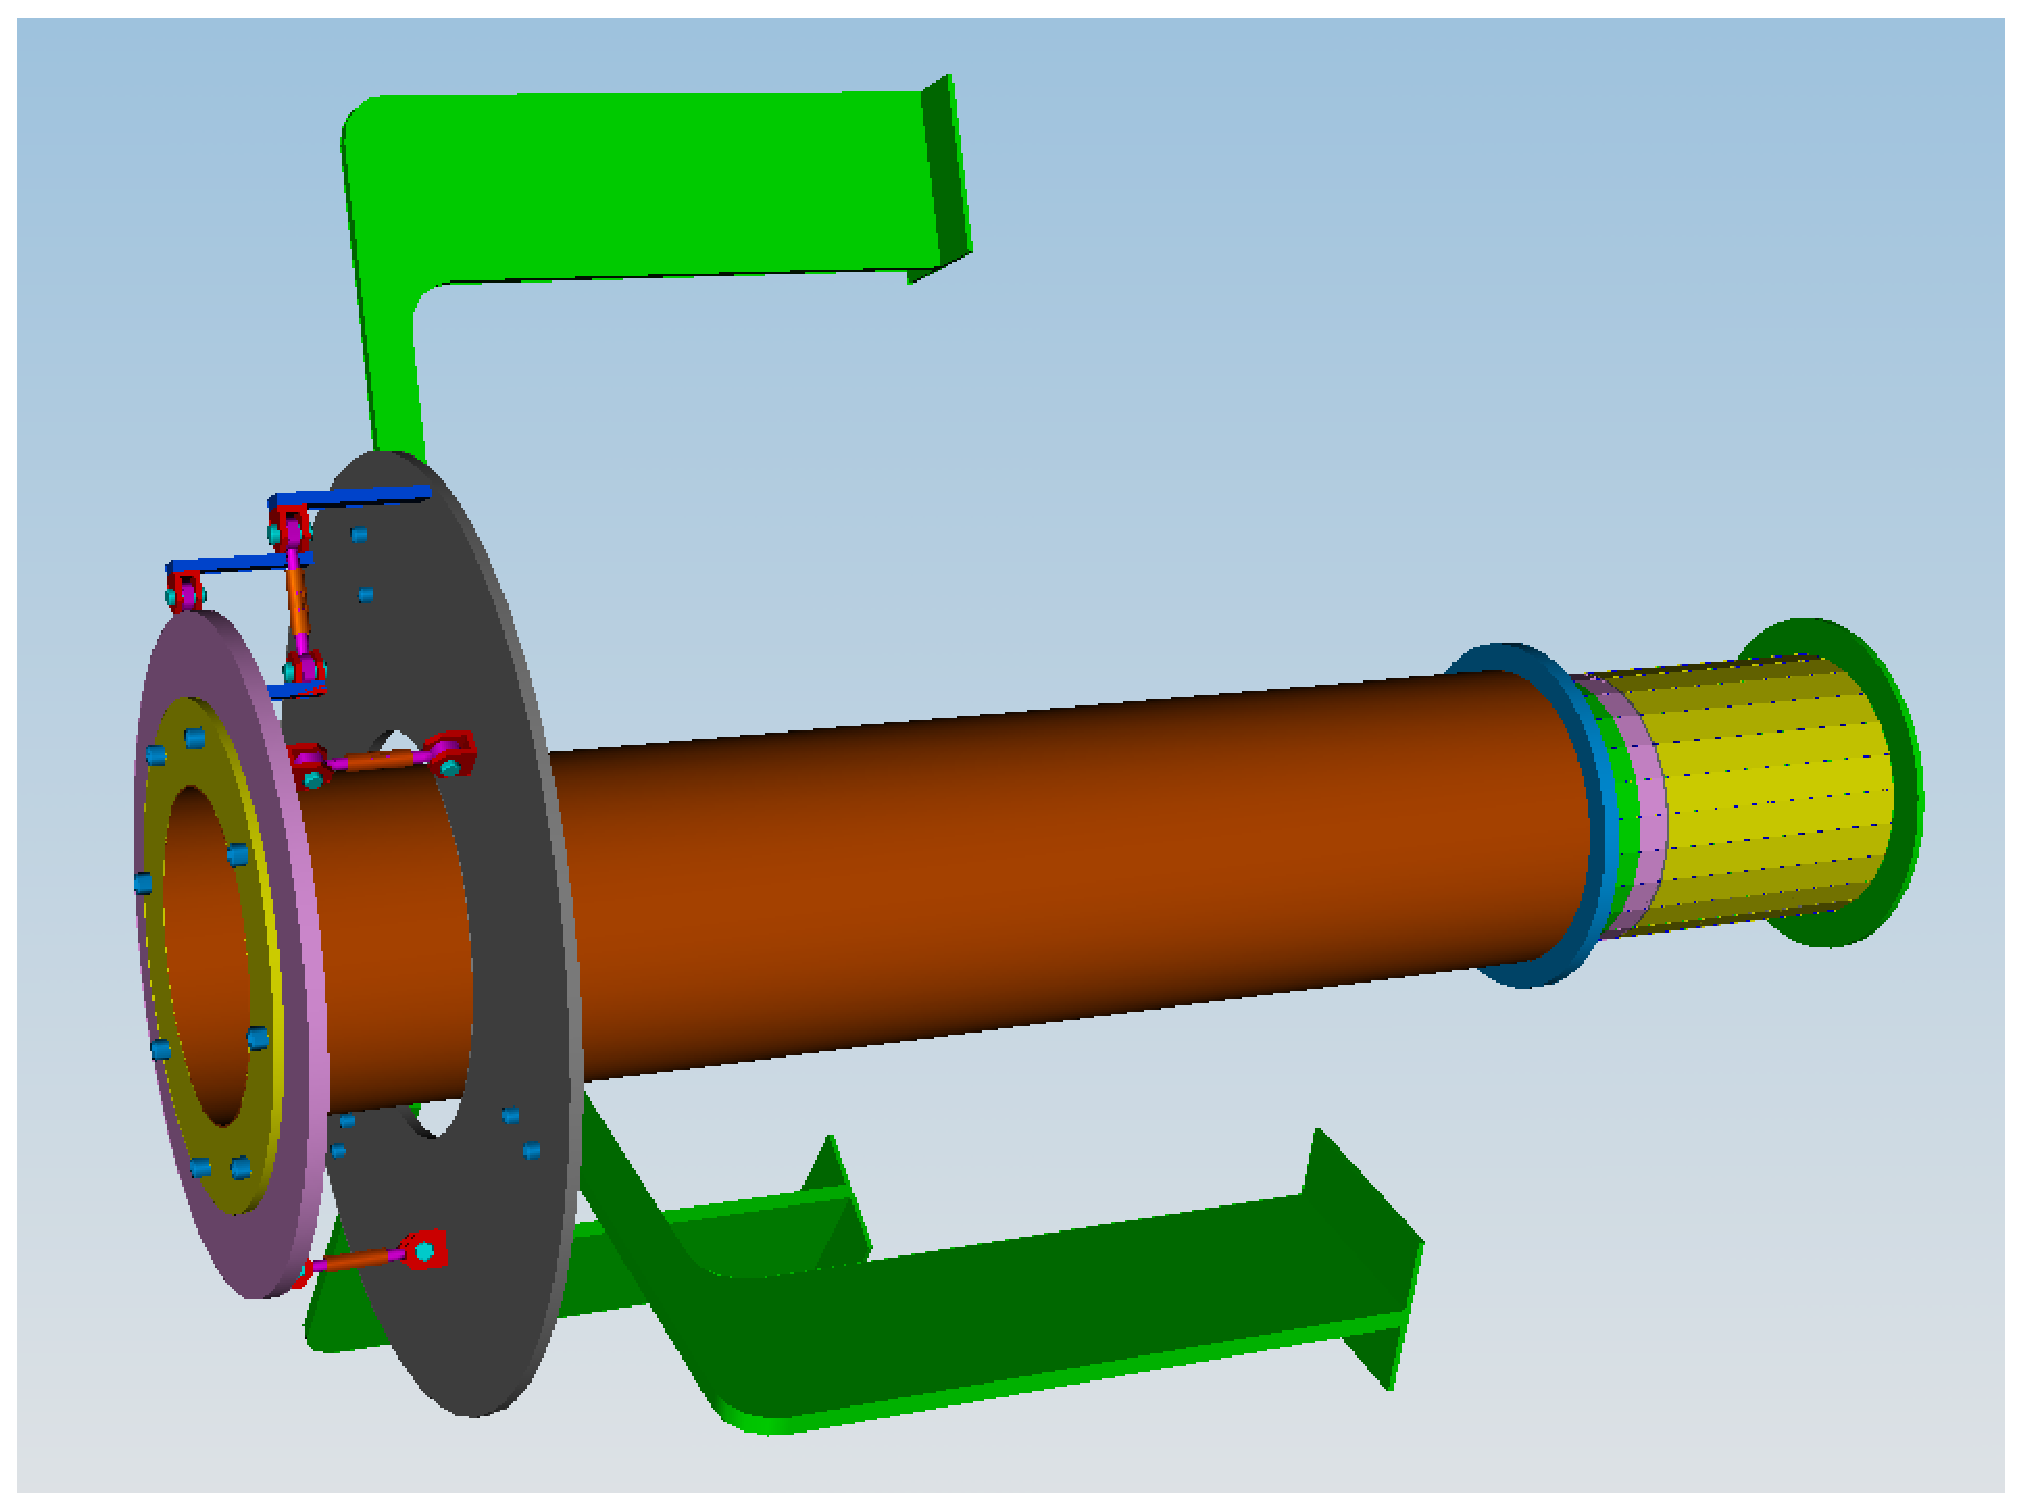
\includegraphics[width=0.60\textwidth]{dave_fig5}
\caption{\small{SVT on support arm with mounting/alignment hardware to
{\tt CLAS12} solenoid.}}
\label{svt_support}
\end{figure}
%%%%%%%%%%%%%%%%%%%%%%%%%%%%%%%%%%%%%%%%%%%%%%%%%%%%%%%%%%%%%%%%%%%%%%%

The relative mass of the support structure is more than 5 times the mass of 
the detector, and it is mounted to the solenoid, which has a mass on the order 
of 20 metric tons, thus vibration will not be an issue.

\subsection{Detector Element Deflection}

Individual staves of the barrel section have been analyzed using ANSYS 
finite element modeling software.  The worst case is Region~1, where its 
deflection is shown in Fig.~\ref{r1_deflect}.  In this modeling, all elements 
of the stave were given both density and stiffness properties, as well as the
dead weight of the electronics (10~g). Deflection of the wafer material can 
be seen to be less than 0.03~mm, which is much less than the required 0.1~mm 
that can cause self induced noise.

%%%%%%%%%%%%%%%%%%%%%%%%%%%%%%%%%%%%%%%%%%%%%%%%%%%%%%%%%%%%%%%%%%%%%%%
\begin{figure}[htbp]
\centering
\includegraphics[width=0.55\textwidth]{dave_ansys1}
\caption{\small{BST Region~1 stave deflection analysis results (units
in mm).}}
\label{r1_deflect}
\end{figure}
%%%%%%%%%%%%%%%%%%%%%%%%%%%%%%%%%%%%%%%%%%%%%%%%%%%%%%%%%%%%%%%%%%%%%%%

\subsection{Detector Element Heat Removal}

Heat removal from the SVT is a significant design issue. The design heat 
load for the SVT is to remove all the on-board electronics heat using 
chilled-water cooling. The total power to be removed is shown in 
Table~\ref{svt_power}.

%%%%%%%%%%%%%%%%%%%%%%%%%%%%%%%%%%%%%%%%%%%%%%%%%%%%%%%%%%%%%%%%%%%%%%%%%
\begin{table}[htbp]
\begin{center}
\begin{tabular} {||l|c|c||} \hline \hline
\multicolumn{3} {|c|} {Heat Load for SVX4}  \\ \hline \hline
Item                       & Barrel & Disk  \\ \hline
No. of modules             & 62     & 45    \\ \hline
Chips/module               & 4      & 8     \\ \hline 
Total chips                & 248    & 360   \\ \hline
Idle power (W)             & 47.6   & 69.1  \\ \hline
Max power/ch (mW/ch)       & 3      & 3     \\ \hline
Max power (W)              & 95.2   & 138.2 \\ \hline
Transceiver power (W)      & 0.5    & 0.5   \\ \hline
No. of transceivers/module & 4      & 4     \\ \hline
Total transceiver power (W)& 124.0  & 90    \\ \hline
Total idle power (W)       & 171.6  & 159.1 \\
(with transceiver)         &        &       \\ \hline
Total max. power (W)       & 219.2  & 228.2 \\
(with transceiver)         &        &       \\ \hline
\end{tabular}
\caption{\small{Heat load on the SVT,}}
\label{svt_power}
\end{center}
\end{table}
%%%%%%%%%%%%%%%%%%%%%%%%%%%%%%%%%%%%%%%%%%%%%%%%%%%%%%%%%%%%%%%%%%%%%%%%%

The primary mode of heat transfer will be conduction heat transfer to a 
water-cooled heat sink.  We have chosen aluminum nitride because it is a 
non-magnetic and electrically non-conductive ceramic material with good 
thermal conductivity.  Two millimeter thick aluminum nitride has been put 
into the core of the staves, replacing the Rohacell core material where 
its mass is not in the acceptance.  Finite element analysis of a Region~4 
module shows that most of the heat can be conducted away, keeping the 
electronics maximum temperature to approximately 40$^\circ$C with the heat 
sink temperature at 15$^\circ$C.  A very small amount of heat (much less 
than 1~W) must be removed from the surface of the wafers to keep them from 
warming to the maximum temperature of the chips.  This can easily be done 
by flushing the detector with a small purge of dry nitrogen.  The temperature 
distribution of a stave in Region~4 is shown in Fig.~\ref{heat_r4}. 

%%%%%%%%%%%%%%%%%%%%%%%%%%%%%%%%%%%%%%%%%%%%%%%%%%%%%%%%%%%%%%%%%%%%%%%
\begin{figure}[htbp]
\centering
\includegraphics[width=0.55\textwidth]{dave_ansys2}
\caption{\small{BST Region~4 stave heat transfer analysis results (units
in $^\circ$C).}}
\label{heat_r4}
\end{figure}
%%%%%%%%%%%%%%%%%%%%%%%%%%%%%%%%%%%%%%%%%%%%%%%%%%%%%%%%%%%%%%%%%%%%%%%

Notice that the temperature along the wafer portion of the stave is around 
23$^\circ$C.  This is because the dry nitrogen that will be purging the 
detector is assumed to be 22$^\circ$C.   Region~1 has a longer conduction 
length, and therefore, higher temperatures are expected.  Two potential 
solutions are being considered.  The first is to use a material with higher 
thermal conductivity (such as a high thermally conductive carbon composite).
The second is to locate the electronics on Region~1 closer to the cooling 
plate.
 
\section{Electronics}

\subsection{Readout}

Both the BST and FST  will be made of single-sided sensors, as single-sided
sensors avoid manufacturing problems and the higher costs associated with
double-sided sensors.  Further, the SVX4 ASIC, a candidate for the readout
electronics, supports single-sided sensors only.  The single-sided sensors
to be used are n-type, AC-coupled, and poly-biased.  After an evaluation of 
the readout ASICs that are available (see Table~\ref{tab:chips}), the 
128-channel SVX4 ASIC that is fabricated on standard 0.25-$\mu$m CMOS 
technology, is considered to be a potential candidate.  SVX4 implements a 
complete readout system and is a low-power device (at 3~mW/channel).  Further, 
the SVX4 ASIC has a good track record and is presently the readout system of 
choice for several single-sided micro-strip detectors.

%%%%%%%%%%%%%%%%%%%%%%%%%%%%%%%%%%%%%%%%%%%%%%%%%%%%%%%%%%%%%%%%%%%%%%%
\begin{table}[htbp]
\begin{center}
\begin{tabular}{|c|c|c|c|c|} \hline
Institution & Experiment & Chip & Manufacturer & Process \\ \hline
CERN & ALICE  & HAL25  & IBM       & 0.25 \\ \hline
CERN & ATLAS  & ABCD   & Honeywell & 0.8  \\ \hline
CERN & CMS    & APV25  & IBM       & 0.25 \\ \hline
CERN & LHCb   & BEETLE & IBM       & 0.25 \\ \hline
FNAL & CDF    & SVX4   & TSMC      & 0.25 \\ \hline
FNAL & D0,CDF & SVX3D  & Honeywell & 0.8  \\ \hline
KEK  & Belle  & VA1TA  & IDEAS     & 0.35 \\ \hline
SLAC & BaBar  & AToM   & Honeywell & 0.8  \\ \hline
\end{tabular}
\end{center}
\caption{\small{Available ASICs that were evaluated for use in {\tt CLAS12}.}}
\label{tab:chips}
\end{table}
%%%%%%%%%%%%%%%%%%%%%%%%%%%%%%%%%%%%%%%%%%%%%%%%%%%%%%%%%%%%%%%%%%%%%%%

As an example of the on-board electronics, a photo-composite of a BST Region~2 
module is shown in Fig.~\ref{fig:module-assembly}.  This assembly is called 
a stave.  Table~\ref{tab:onboard-electronics} lists the significant components 
of the on-detector electronics.  The operating bias voltage is expected to be 
$\sim$200~V.  For low thermal noise and production uniformity, the 
poly-silicon bias resistor is required to be $\sim$2.5~M$\Omega$.  The 
inter-strip resistance is expected to be $\sim$1~G$\Omega$.  To minimize 
signal dispersion, a strip resistance of less than 30~$\Omega$/cm is desirable.

%%%%%%%%%%%%%%%%%%%%%%%%%%%%%%%%%%%%%%%%%%%%%%%%%%%%%%%%%%%%%%%%%%%%%%%
\begin{figure}[htbp]
\centering
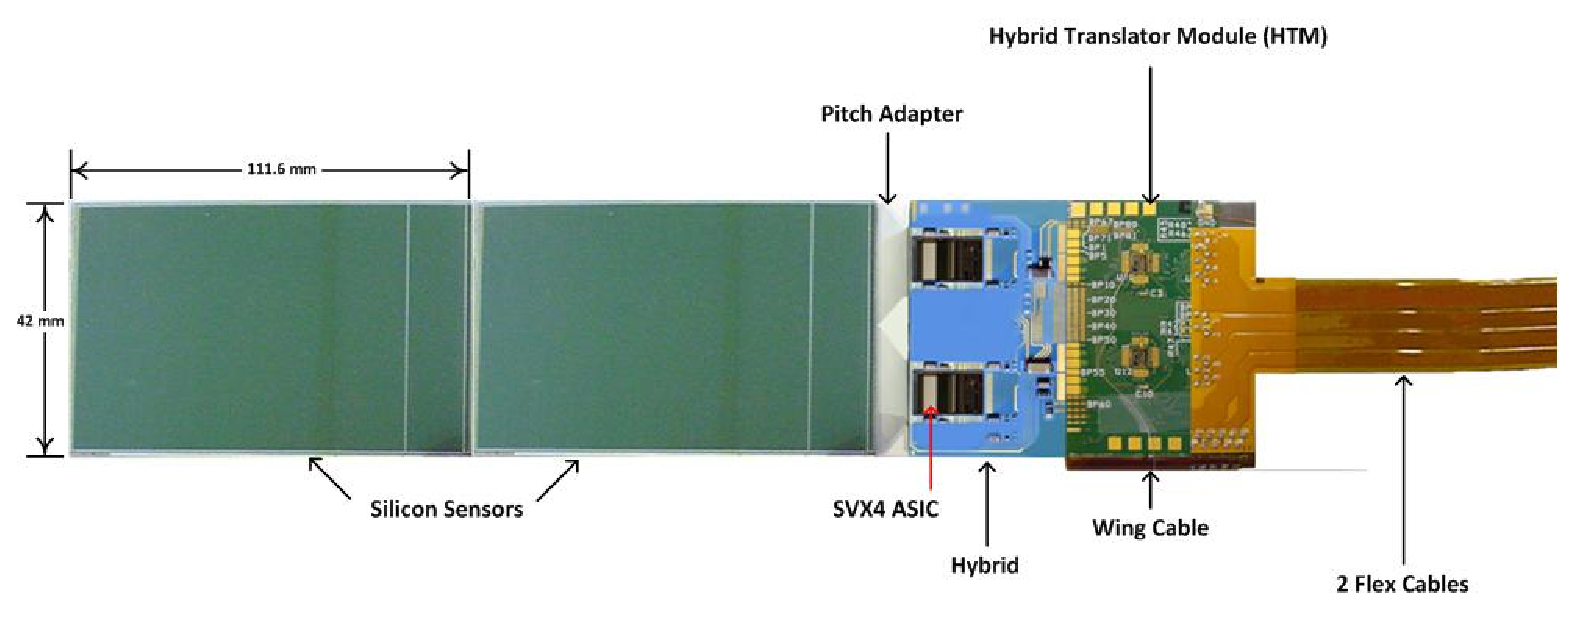
\includegraphics[width=0.85\textwidth]{module-assembly}
\caption{\small{Photo-composite of a Region~2 barrel module stave assembly.}}
\label{fig:module-assembly}
\end{figure}
%%%%%%%%%%%%%%%%%%%%%%%%%%%%%%%%%%%%%%%%%%%%%%%%%%%%%%%%%%%%%%%%%%%%%%%

%%%%%%%%%%%%%%%%%%%%%%%%%%%%%%%%%%%%%%%%%%%%%%%%%%%%%%%%%%%%%%%%%%%%%%%
\begin{table}[htbp]
\begin{center}
\begin{small}
\begin{tabular}{|l|l|l|} \hline
Component       & Basic Specifications & Function \\ \hline
Silicon sensors & Single sided, 300-$\mu$m thick, 42~mm$\times$111.62~mm (cut),
 &   \\
                & 75~$\mu$m implant pitch, 150~$\mu$m readout pitch, $V/W$ & Charge collection \\
                & layers $\pm$1.5$^\circ$, $n$-type, 2 sensors from a 6-in wafer &  \\ \hline
Pitch adapters  & Adapts SVX4 48-$\mu$m pitch to sensor 150-$\mu$m readout 
 & Hybrid to sensor \\
                & pitch       & Connection \\ \hline
Hybrids         & BeO substrate, $\sim$38~mm$\times$20~mm, bonding pads for 
  & SVX4 ASIC mounting\\
                & 2 SVX4 ASICs &  \\ \hline
Hybrid Translator & LVDS signal transceivers, $\sim$40~mm$\times$40~mm 
(smaller & Translates and repeats \\
Module (HTM)    & if possible)            & module control and \\
                &                         & data signals \\ \hline
Wing cable & Flex cable extension of HTM circuit board, & Connects signals from \\
                & wire-bond pads for bottom hybrid & top to bottom HTM \\ \hline
\end{tabular}
\end{small}
\end{center}
\caption{\small{Significant components of the on-board electronics.}}
\label{tab:onboard-electronics}
\end{table}
%%%%%%%%%%%%%%%%%%%%%%%%%%%%%%%%%%%%%%%%%%%%%%%%%%%%%%%%%%%%%%%%%%%%%%%

The SVX4 design handles sensor capacitances from 10~pF to 35~pF.  For the
FST and the BST, the total inter-strip capacitance is expected to be
$\le$1.2~pF/cm and the coupling capacitance is expected to be
$\ge$10~pF/cm for AC-coupled strips.  The equivalent noise charge (ENC) in 
a channel is given by ENC = $400 e^- + 42 e^-/$~pF.  For a capacitance of 
30~pF, the typical capacitance of a long strip, plus some additional stray 
capacitance due to the wire-bonds connecting the sensor and the chip, ENC 
is estimated to be 1800$e^-$.  This noise level is about a tenth of the 
signal level generated by a minimum ionizing particle.

Fig.~\ref{fig:svx-channel-sch} shows a block diagram of a single SVX4 
channel.  The detector signals are integrated, correlated double samples, 
the difference of which is stored in the analog pipeline.  Up to 42 
measurements can be stored in the pipeline.  Digitization is by means of a 
Wilkinson-type ADC and an 8-bit counter.  Timing control signals govern, 
among other functions, the operation of each channel's preamp reset, the 
double-correlated sampling, and the ADC.  These timing control signals must 
be generated by a trigger generated by other detectors in {\tt CLAS12}.
Once a pipeline cell is marked by the Level-1 accept (L1A) trigger, the 
counter value is stored in a FIFO buffer.  An 8-bit output bus transmits 
the data in a sequence of bytes identifying the chip, pipeline cell, the 
channel number, and the content.

%%%%%%%%%%%%%%%%%%%%%%%%%%%%%%%%%%%%%%%%%%%%%%%%%%%%%%%%%%%%%%%%%%%%%%%
\begin{figure}[htbp]
\vspace{5.7cm}
\special{psfile=svx-channel-sch.eps hscale=55 vscale=55 
hoffset=40 voffset=-5}
\caption{\small{Schematic of an SVX4 chip showing the layout for the
preamp, through the pipeline and ADC to the FIFO buffer.}}
\label{fig:svx-channel-sch}
\end{figure}
%%%%%%%%%%%%%%%%%%%%%%%%%%%%%%%%%%%%%%%%%%%%%%%%%%%%%%%%%%%%%%%%%%%%%%%

%%%%%%%%%%%%%%%%%%%%%%%%%%%%%%%%%%%%%%%%%%%%%%%%%%%%%%%%%%%%%%%%%%%%%%%
\begin{figure}[htbp]
\centering
\includegraphics[width=0.5\textwidth]{svx-floorplan}
\caption{\small{SVX4 ASIC floor plan.}}
\label{fig:svx-floorplan}
\end{figure}
%%%%%%%%%%%%%%%%%%%%%%%%%%%%%%%%%%%%%%%%%%%%%%%%%%%%%%%%%%%%%%%%%%%%%%%

Fig.~\ref{fig:svx-floorplan} shows the floor plan of the SVX4 ASIC.
The thickness of the chip is 0.25~mm.  The diced area of the chip is 
6.40~mm $\times$ 9.11~mm.  The channel input pads are 0.096~mm apart, 
center-to-center, and the pad widths are 0.048~mm.  There are two rows 
of input pads to which the outputs of the silicon sensors have to be 
wire-bonded.  Pitch adapters connect the sensor and the hybrid.  Wire-bond 
pads are located on both ends of the pitch adapter for connections to the 
SVX4 ASICs and to the sensor.  The wire-bonding pads will be compatible 
with the aluminum-wire ultrasonic wedge-bonding method.  A separate ceramic
pitch adapter will be glued onto the module support assembly.
Fig.~\ref{fig:pitch-adapter} shows the pitch adapter connections to the 
sensor and SVX4 ASICs.  Fiducial marks will be made on the pitch adapter
for assembly and alignment.  In addition to routing the sensor signals and 
the guard ground, the high voltage will be routed across the pitch adapter 
from the hybrid to the sensor bias ring.  Adequate spacing between the pitch 
adapter, high voltage trace, sensor guard, and ground will be provided.

%%%%%%%%%%%%%%%%%%%%%%%%%%%%%%%%%%%%%%%%%%%%%%%%%%%%%%%%%%%%%%%%%%%%%%%
\begin{figure}[htbp]
\centering
\includegraphics[width=0.65\textwidth]{pitch-adapter}
\caption{\small{Pitch adapter connections to the sensor.}}
\label{fig:pitch-adapter}
\end{figure}
%%%%%%%%%%%%%%%%%%%%%%%%%%%%%%%%%%%%%%%%%%%%%%%%%%%%%%%%%%%%%%%%%%%%%%%

Fig.~\ref{fig:hybrid} shows a photo-composite of the proposed hybrid for
mounting the SVX4 chips.  The hybrid will be outside of the active area, 
not on the sensor, and glued directly onto the support structure.  The 
proposed hybrid with approximate dimensions of 38~mm $\times$ 20~mm will 
be used to mount the two SVX4 readout ASICs.  The hybrid substrate uses 
beryllium oxide, which is a good heat conductor and has a long radiation 
length.  The gold bond pads of the hybrid will be aluminum-wedge bondable 
to be compatible with the other components.  The high voltage for the 
sensors will be routed across the hybrid with an adequate wire-bonding 
surface for connections to the pitch adapter and the hybrid translator 
module (HTM).  An RTD (resistance temperature detector) will be mounted 
on the hybrid for temperature measurements.

%%%%%%%%%%%%%%%%%%%%%%%%%%%%%%%%%%%%%%%%%%%%%%%%%%%%%%%%%%%%%%%%%%%%%%%
\begin{figure}[htbp]
\centering
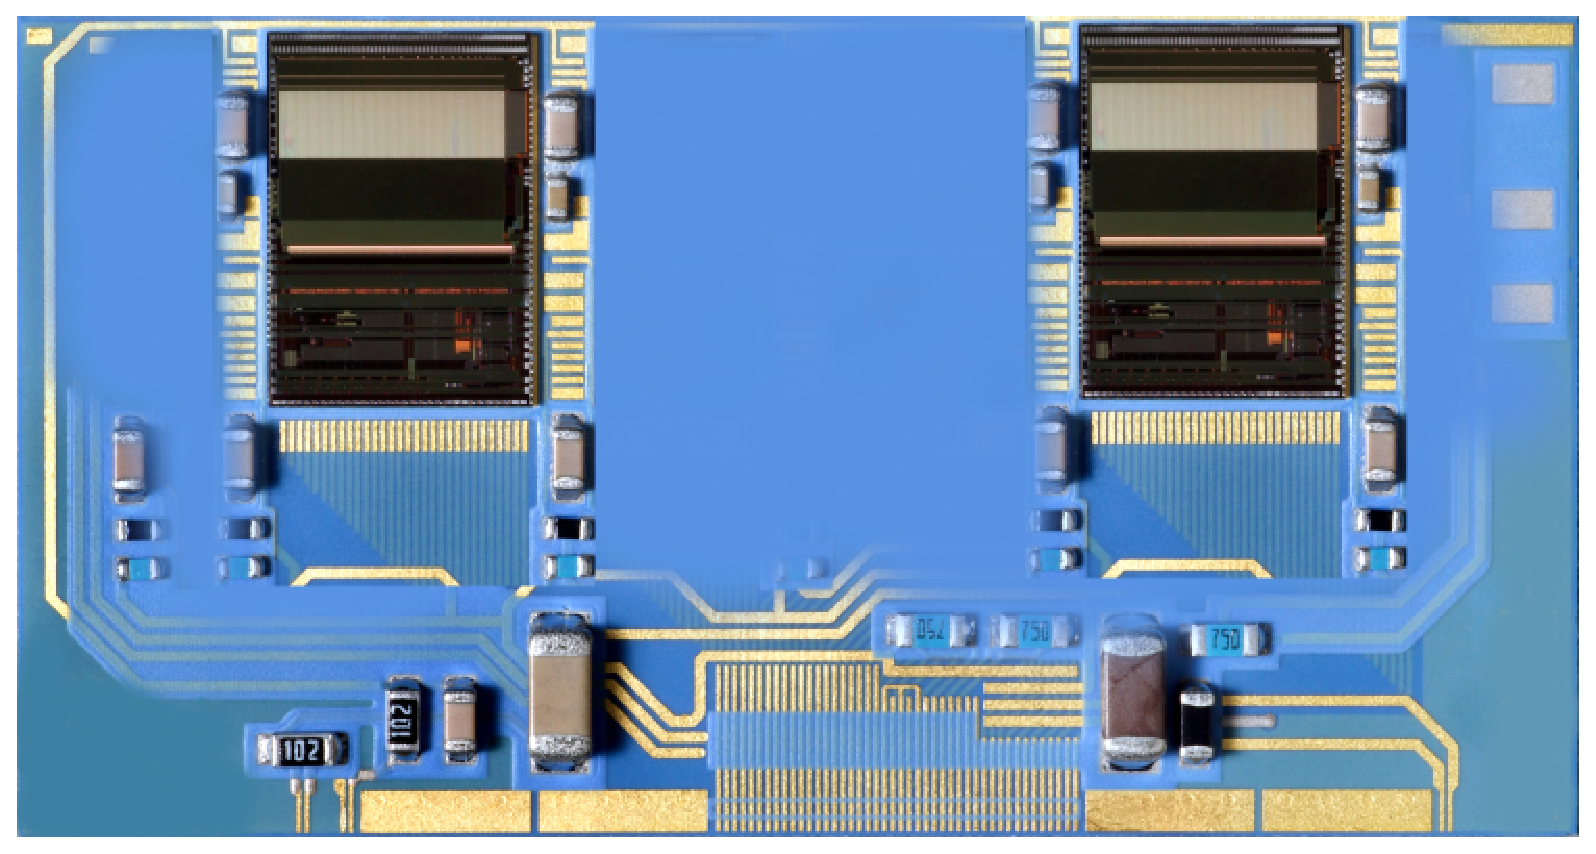
\includegraphics[width=0.5\textwidth]{hybrid}
\caption{\small{Photo-composite of the hybrid board for mounting of the
SVX4 chips.}}
\label{fig:hybrid}
\end{figure}
%%%%%%%%%%%%%%%%%%%%%%%%%%%%%%%%%%%%%%%%%%%%%%%%%%%%%%%%%%%%%%%%%%%%%%%

Separate power supplies and grounds for the analog and digital sections 
will be used.  The dielectric strength of the circuit board will be 
$\geq$650~V/mil.  SVX4 diagnostic signals have external pull-up resistors 
and will be routed to the hybrid test points.  Fig.~\ref{fig:hybrid-sch} 
shows a conceptual schematic of the hybrid based on the FNAL CDF design.

%%%%%%%%%%%%%%%%%%%%%%%%%%%%%%%%%%%%%%%%%%%%%%%%%%%%%%%%%%%%%%%%%%%%%%%
\begin{figure}[htbp]
\centering
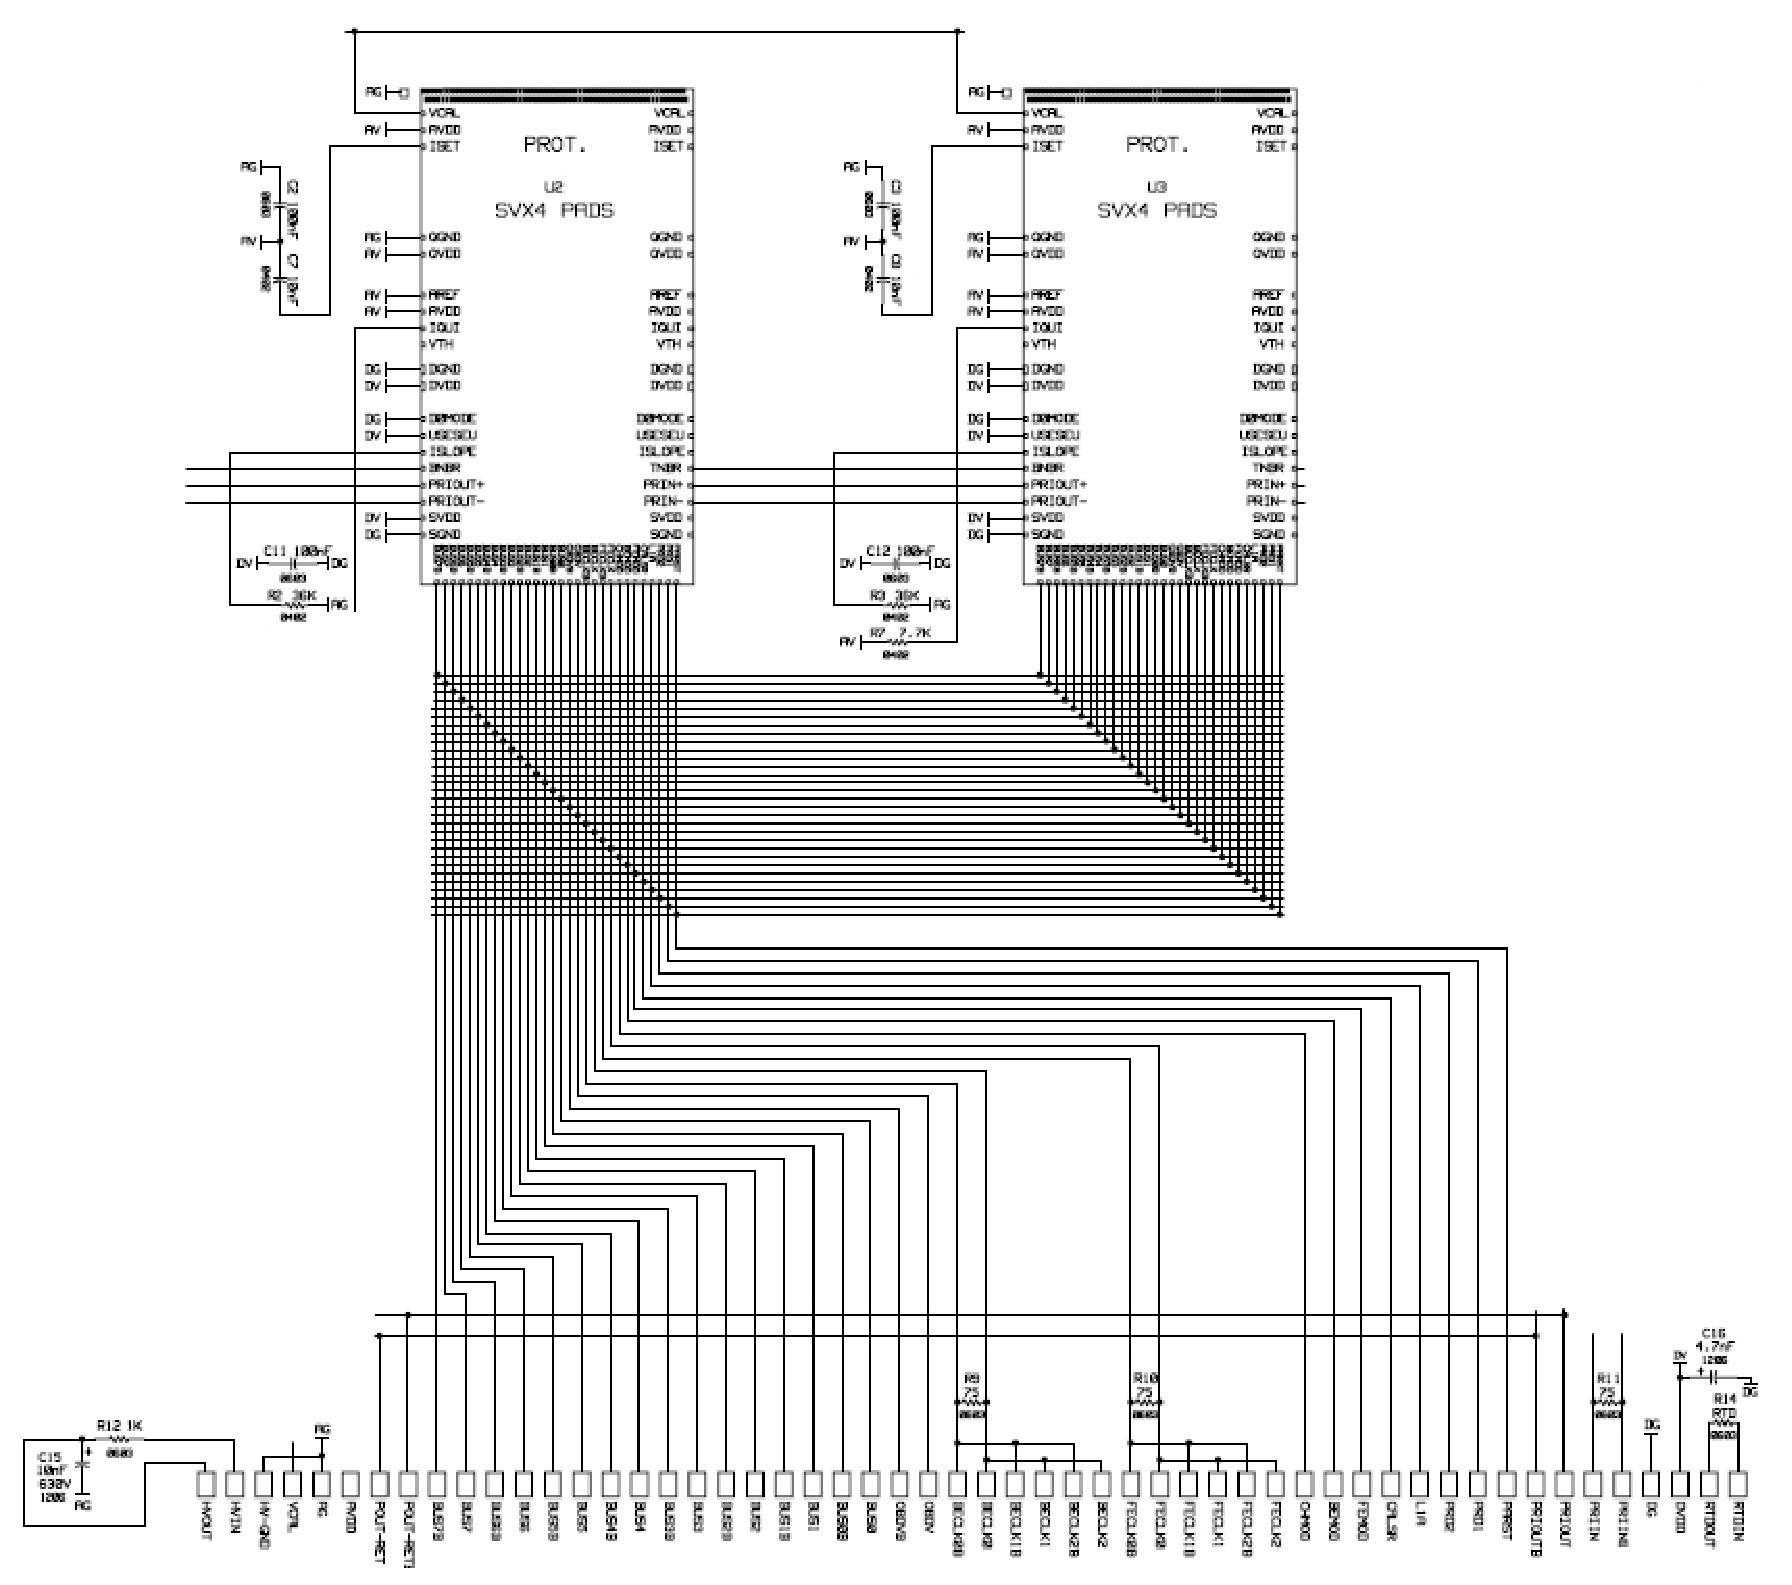
\includegraphics[width=0.9\textwidth]{hybrid-sch}
\caption{\small{Conceptual schematic of the hybrid board layout of the
SVT.}}
\label{fig:hybrid-sch}
\end{figure}
%%%%%%%%%%%%%%%%%%%%%%%%%%%%%%%%%%%%%%%%%%%%%%%%%%%%%%%%%%%%%%%%%%%%%%%

The connections for the priority in - priority out SVX4 readout chain 
allow for reading the top side and then the bottom side of the module.
The input and output for the readout chain are then routed to HTM 
transceivers and then to the external connectors.  The HTM translates and 
repeats control and data signals from the two hybrids on a module to the 
DAQ.  The HTM also routes the low voltage and high voltage supply lines 
from the flex cables to the hybrid.  Fig.~\ref{fig:readout-chain} shows a 
conceptual block diagram of the SVX4 readout chain.  Fig.~\ref{htm} (top) 
shows a FNAL HTM that has the dimensions of 39~mm $\times$ 50~mm; at JLab 
a smaller module ($\sim$40~mm $\times$ 30~mm or less) is being developed 
for {\tt CLAS12}.  Fig.~\ref{htm} (bottom) shows a block diagram of the 
HTM board.  The FNAL 10-bit low voltage differential signal ASIC 
transceiver will be used because of its high density and its good track 
record with silicon-strip detectors.  The transceiver comes in die form 
and is wire-bonded to the HTM board.

%%%%%%%%%%%%%%%%%%%%%%%%%%%%%%%%%%%%%%%%%%%%%%%%%%%%%%%%%%%%%%%%%%%%%%%
\begin{figure}[htbp]
\centering
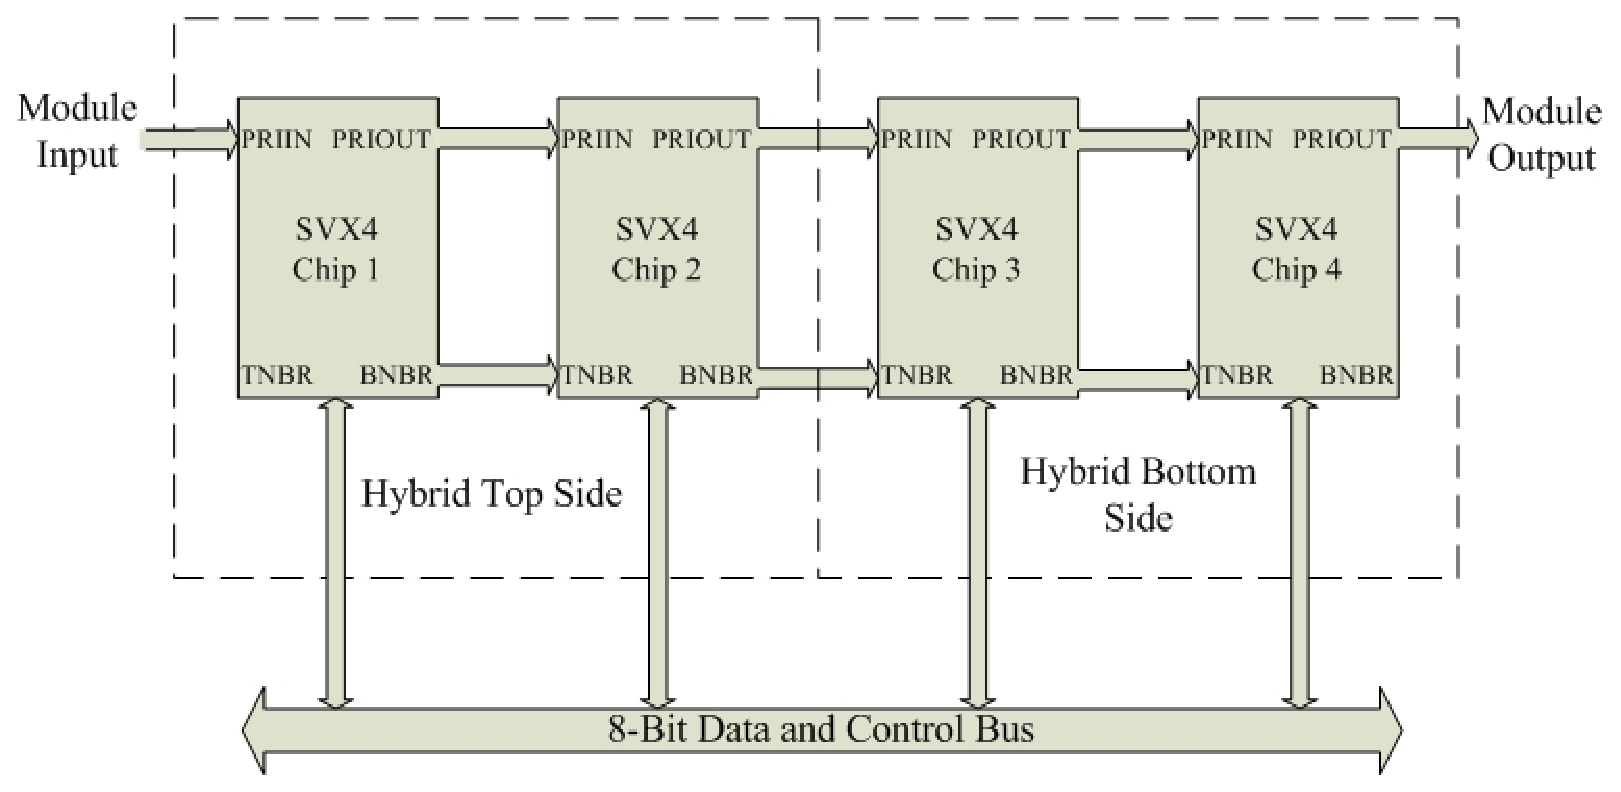
\includegraphics[width=0.75\textwidth]{readout-chain}
\caption{\small{SVX4 readout chain configuration.}}
\label{fig:readout-chain}
\end{figure}
%%%%%%%%%%%%%%%%%%%%%%%%%%%%%%%%%%%%%%%%%%%%%%%%%%%%%%%%%%%%%%%%%%%%%%%

%%%%%%%%%%%%%%%%%%%%%%%%%%%%%%%%%%%%%%%%%%%%%%%%%%%%%%%%%%%%%%%%%%%%%%%
\begin{figure}[htbp]
\vspace{13.5cm}
\special{psfile=htm-top.eps hscale=45 vscale=45 hoffset=20 voffset=235}
\special{psfile=htm-sch.eps hscale=40 vscale=40 hoffset=210 voffset=0}
\caption{\small{(Top) Top side view of the hybrid translator module (HTM).
(Bottom) Corresponding block diagram for the HTM board.}}
\label{htm}
\end{figure}
%%%%%%%%%%%%%%%%%%%%%%%%%%%%%%%%%%%%%%%%%%%%%%%%%%%%%%%%%%%%%%%%%%%%%%%

The ``wing'' cable connects the bottom-side hybrid to the transceiver on 
the HTM board.  The wing cable and the HTM will be combined together into 
a single polyimide rigid (HTM) and flex (wing cable) assembly.  In addition 
to the wing cable, the two flex cables with the data, low voltage, and high 
voltage connectors will be attached to the HTM board.  
Fig.~\ref{fig:wing-cable} shows the wing cable on bottom side of the module.  
Fig.~\ref{fig:htm} shows the HTM board and wing cable before folding.
Fig.~\ref{fig:flex-cable} shows the flex cable assembly.  The length of 
the cable is limited to $\sim$30~cm.  Fig.~\ref{routing} shows the flow of 
the cables.  All cables will be routed to the electronic racks located at 
the rear of the detector.

%%%%%%%%%%%%%%%%%%%%%%%%%%%%%%%%%%%%%%%%%%%%%%%%%%%%%%%%%%%%%%%%%%%%%%%
\begin{figure}[htbp]
\centering
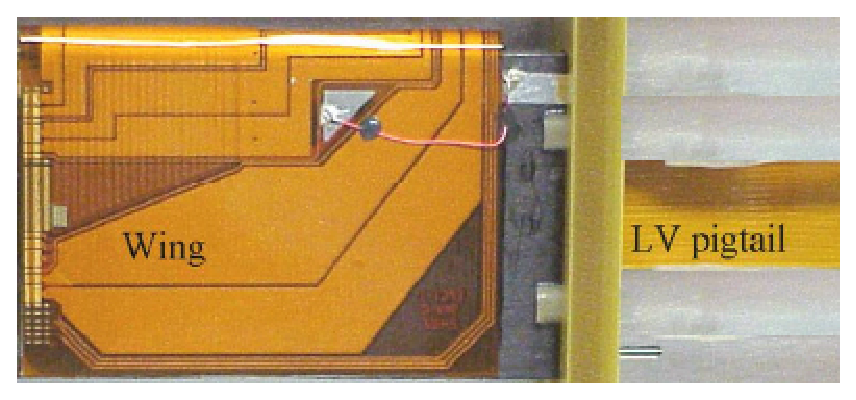
\includegraphics[width=0.65\textwidth]{wing-cable}
\caption{\small{Wing cable on the bottom of the HTM board.}}
\label{fig:wing-cable}
\end{figure}
%%%%%%%%%%%%%%%%%%%%%%%%%%%%%%%%%%%%%%%%%%%%%%%%%%%%%%%%%%%%%%%%%%%%%%%

%%%%%%%%%%%%%%%%%%%%%%%%%%%%%%%%%%%%%%%%%%%%%%%%%%%%%%%%%%%%%%%%%%%%%%%
\begin{figure}[htbp]
\centering
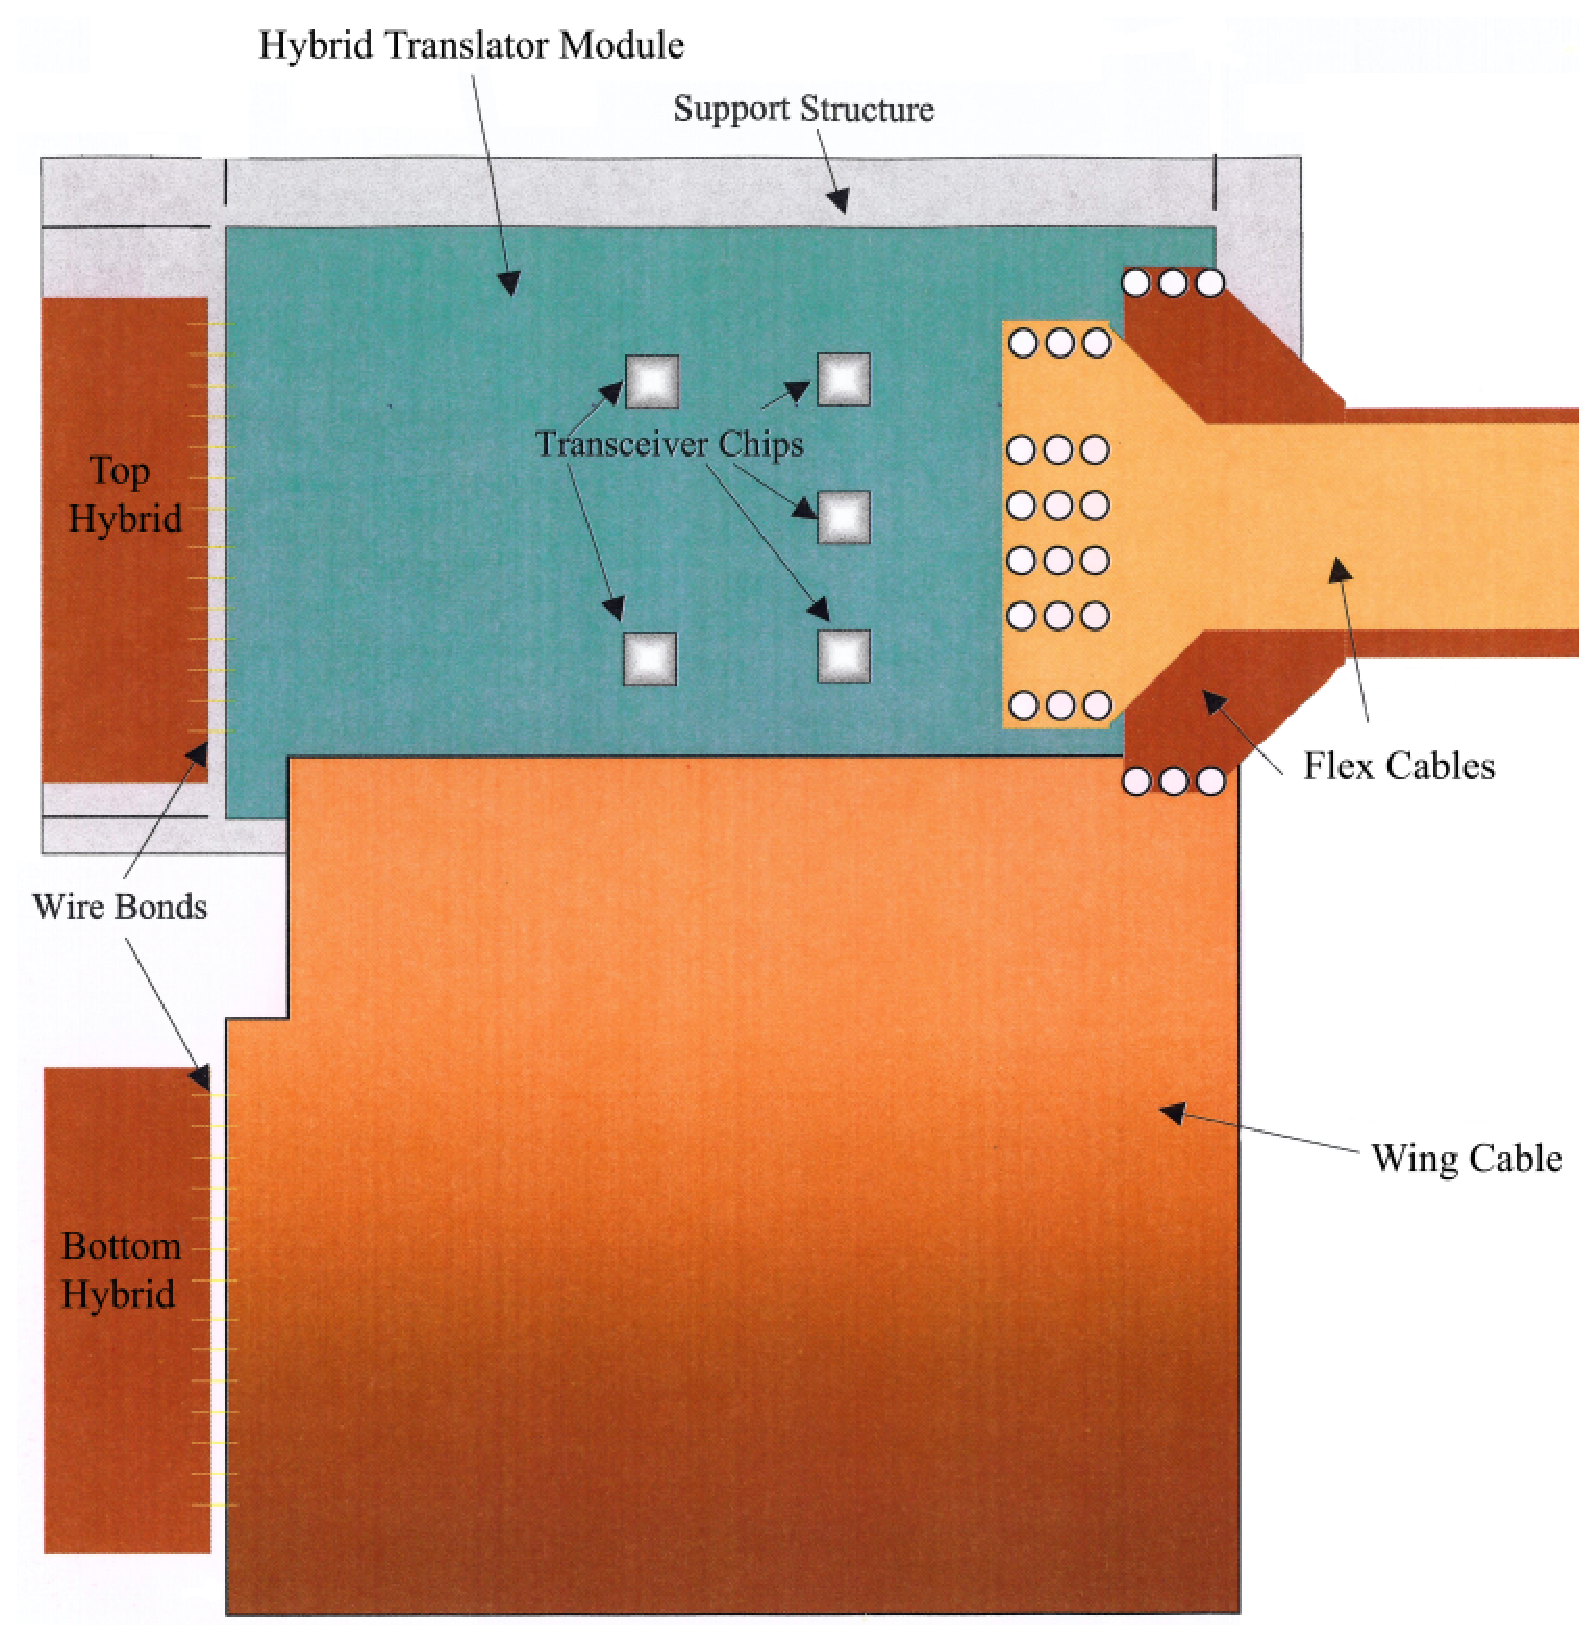
\includegraphics[width=0.5\textwidth]{htm}
\caption{\small{HTM assembly showing the wing cable to connect the top
and bottom side boards and the readout flex cable.}}
\label{fig:htm}
\end{figure}
%%%%%%%%%%%%%%%%%%%%%%%%%%%%%%%%%%%%%%%%%%%%%%%%%%%%%%%%%%%%%%%%%%%%%%%

%%%%%%%%%%%%%%%%%%%%%%%%%%%%%%%%%%%%%%%%%%%%%%%%%%%%%%%%%%%%%%%%%%%%%%%
\begin{figure}[htbp]
\centering
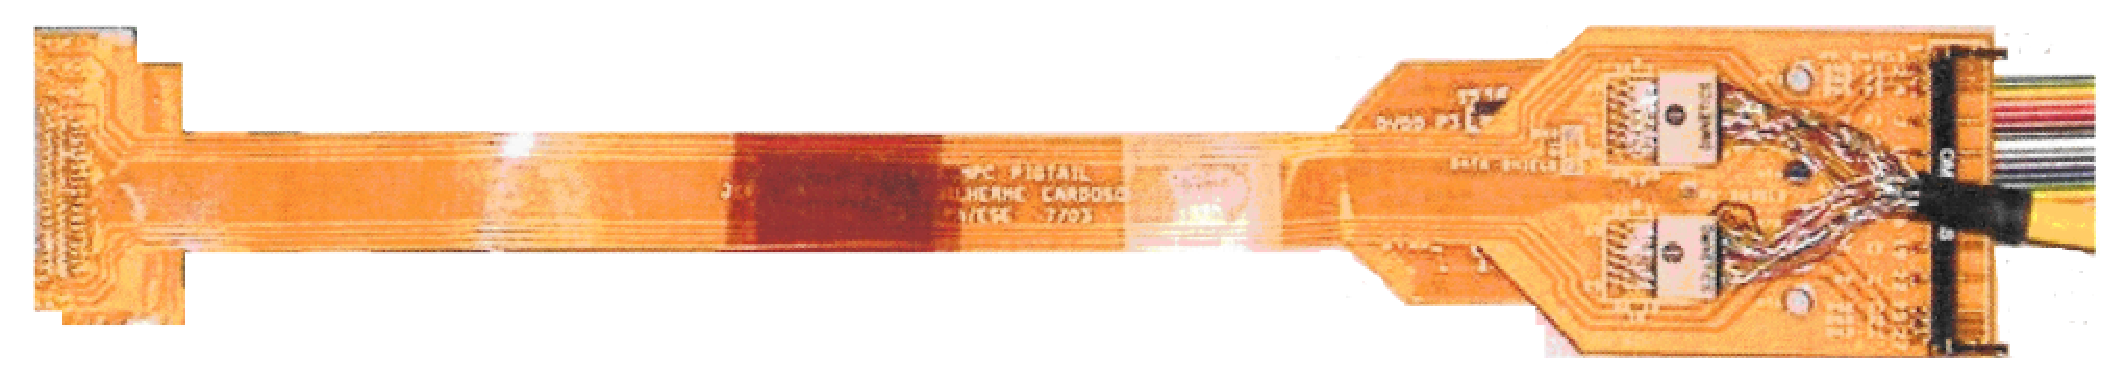
\includegraphics[width=\textwidth]{flex-cable}
\caption{\small{Photograph of the flex cable assembly.}}
\label{fig:flex-cable}
\end{figure}
%%%%%%%%%%%%%%%%%%%%%%%%%%%%%%%%%%%%%%%%%%%%%%%%%%%%%%%%%%%%%%%%%%%%%%%

%%%%%%%%%%%%%%%%%%%%%%%%%%%%%%%%%%%%%%%%%%%%%%%%%%%%%%%%%%%%%%%%%%%%%%%
\begin{figure}[htbp]
\vspace{8.5cm}
\special{psfile=cable-route.eps hscale=22 vscale=22 hoffset=85 
voffset=10}
\caption{\small{Cable routing diagram for the SVT detector.}}
\label{routing}
\end{figure}
%%%%%%%%%%%%%%%%%%%%%%%%%%%%%%%%%%%%%%%%%%%%%%%%%%%%%%%%%%%%%%%%%%%%%%%

\subsection{High and Low Voltage}

The system is designed with the highest low voltage and high voltage 
segmentation affordable, without compromising performance and operability.
Each side of the module has its own high voltage channel, two high voltage 
channels per module.  The five channels of low voltage for the module 
consist of a hybrid analog and a hybrid digital channel for the top and 
for the bottom sides of the sensor module and a digital channel for the HTM.
All of these channels operate at 2.5~V.  In addition to the low voltage and 
high voltage, a calibration voltage for each of the two hybrids connects to 
the flex cable low voltage connector.

The low voltage system consists of $\sim$625 channels in four groups.  The 
high voltage system has $\sim$240 channels.  Fig.~\ref{fig:system-connections}
shows the distribution of voltage and monitoring channels for the SVT.  The 
low voltage and high voltage supplies for the SVT will be modular with 
individual channels provided by a module within a main supply crate.  
Sensors will have a controllable and monitorable high voltage channel with 
over-current and over-voltage trip protection.  A calibration signal and a 
temperature sensor on each hybrid will be instrumented on the detector 
modules.  Table~\ref{tab:voltages} shows the distribution of low and high 
voltage channels needed for the sensors, the HTMs, and the sector collector 
modules (SCM). 

%%%%%%%%%%%%%%%%%%%%%%%%%%%%%%%%%%%%%%%%%%%%%%%%%%%%%%%%%%%%%%%%%%%%%%%
\begin{table}[htbp]
\begin{center}
\begin{small}
\begin{tabular}{|c|c|c|c|c|c|} \hline
Specification & Region 1 & Region 2 & Region 3 & Region 4 & Total \\ \hline
Hybrid 2.5 V digital channels (barrel) & 14 & 24 & 34 & 44 & 116 \\ \hline
Hybrid 2.5 V digital channels (nose cone) & 40 & 42 & 42 & 0 & 124 \\ \hline
Hybrid 2.5 V analog channels (barrel) & 14 & 24 & 34 & 44 & 116 \\ \hline
Hybrid 2.5 V analog channels (nose cone) & 40 & 42 & 42 & 0 & 124 \\ \hline
HTM LV channels (barrel) & 7 & 12 & 17 & 22 & 58 \\ \hline
HTM LV channels (nose cone) & 20 & 21 & 21 & 0 & 62 \\ \hline
SCM LV channels (barrel) & 2 & 3 & 4 & 4 & 13 \\ \hline
SCM LV channels (nose cone) & 4 & 5 & 5 & 0 & 14 \\ \hline
HV channels (barrel) & 14 & 24 & 34 & 44 & 116 \\ \hline
HV channels (nose cone) & 40 & 42 & 42 & 0 & 124 \\ \hline \hline
\end{tabular}
\end{small}
\end{center}
\caption{\small{High and low voltage channel distribution for the SVT.}}
\label{tab:voltages}
\end{table}
%%%%%%%%%%%%%%%%%%%%%%%%%%%%%%%%%%%%%%%%%%%%%%%%%%%%%%%%%%%%%%%%%%%%%%%

The CAEN crate-based high voltage systems, including the 1527 and 1527LC, 
and the WIENER universal multi-channel modular system for both low voltage 
and high voltage supply are being considered.  The WIENER modular system 
has the advantage of a common crate that will support both high voltage 
and low voltage modules.  Fig.~\ref{fig:system-connections} shows an 
overview of the connections of the system.

%%%%%%%%%%%%%%%%%%%%%%%%%%%%%%%%%%%%%%%%%%%%%%%%%%%%%%%%%%%%%%%%%%%%%%%
\begin{figure}[htbp]
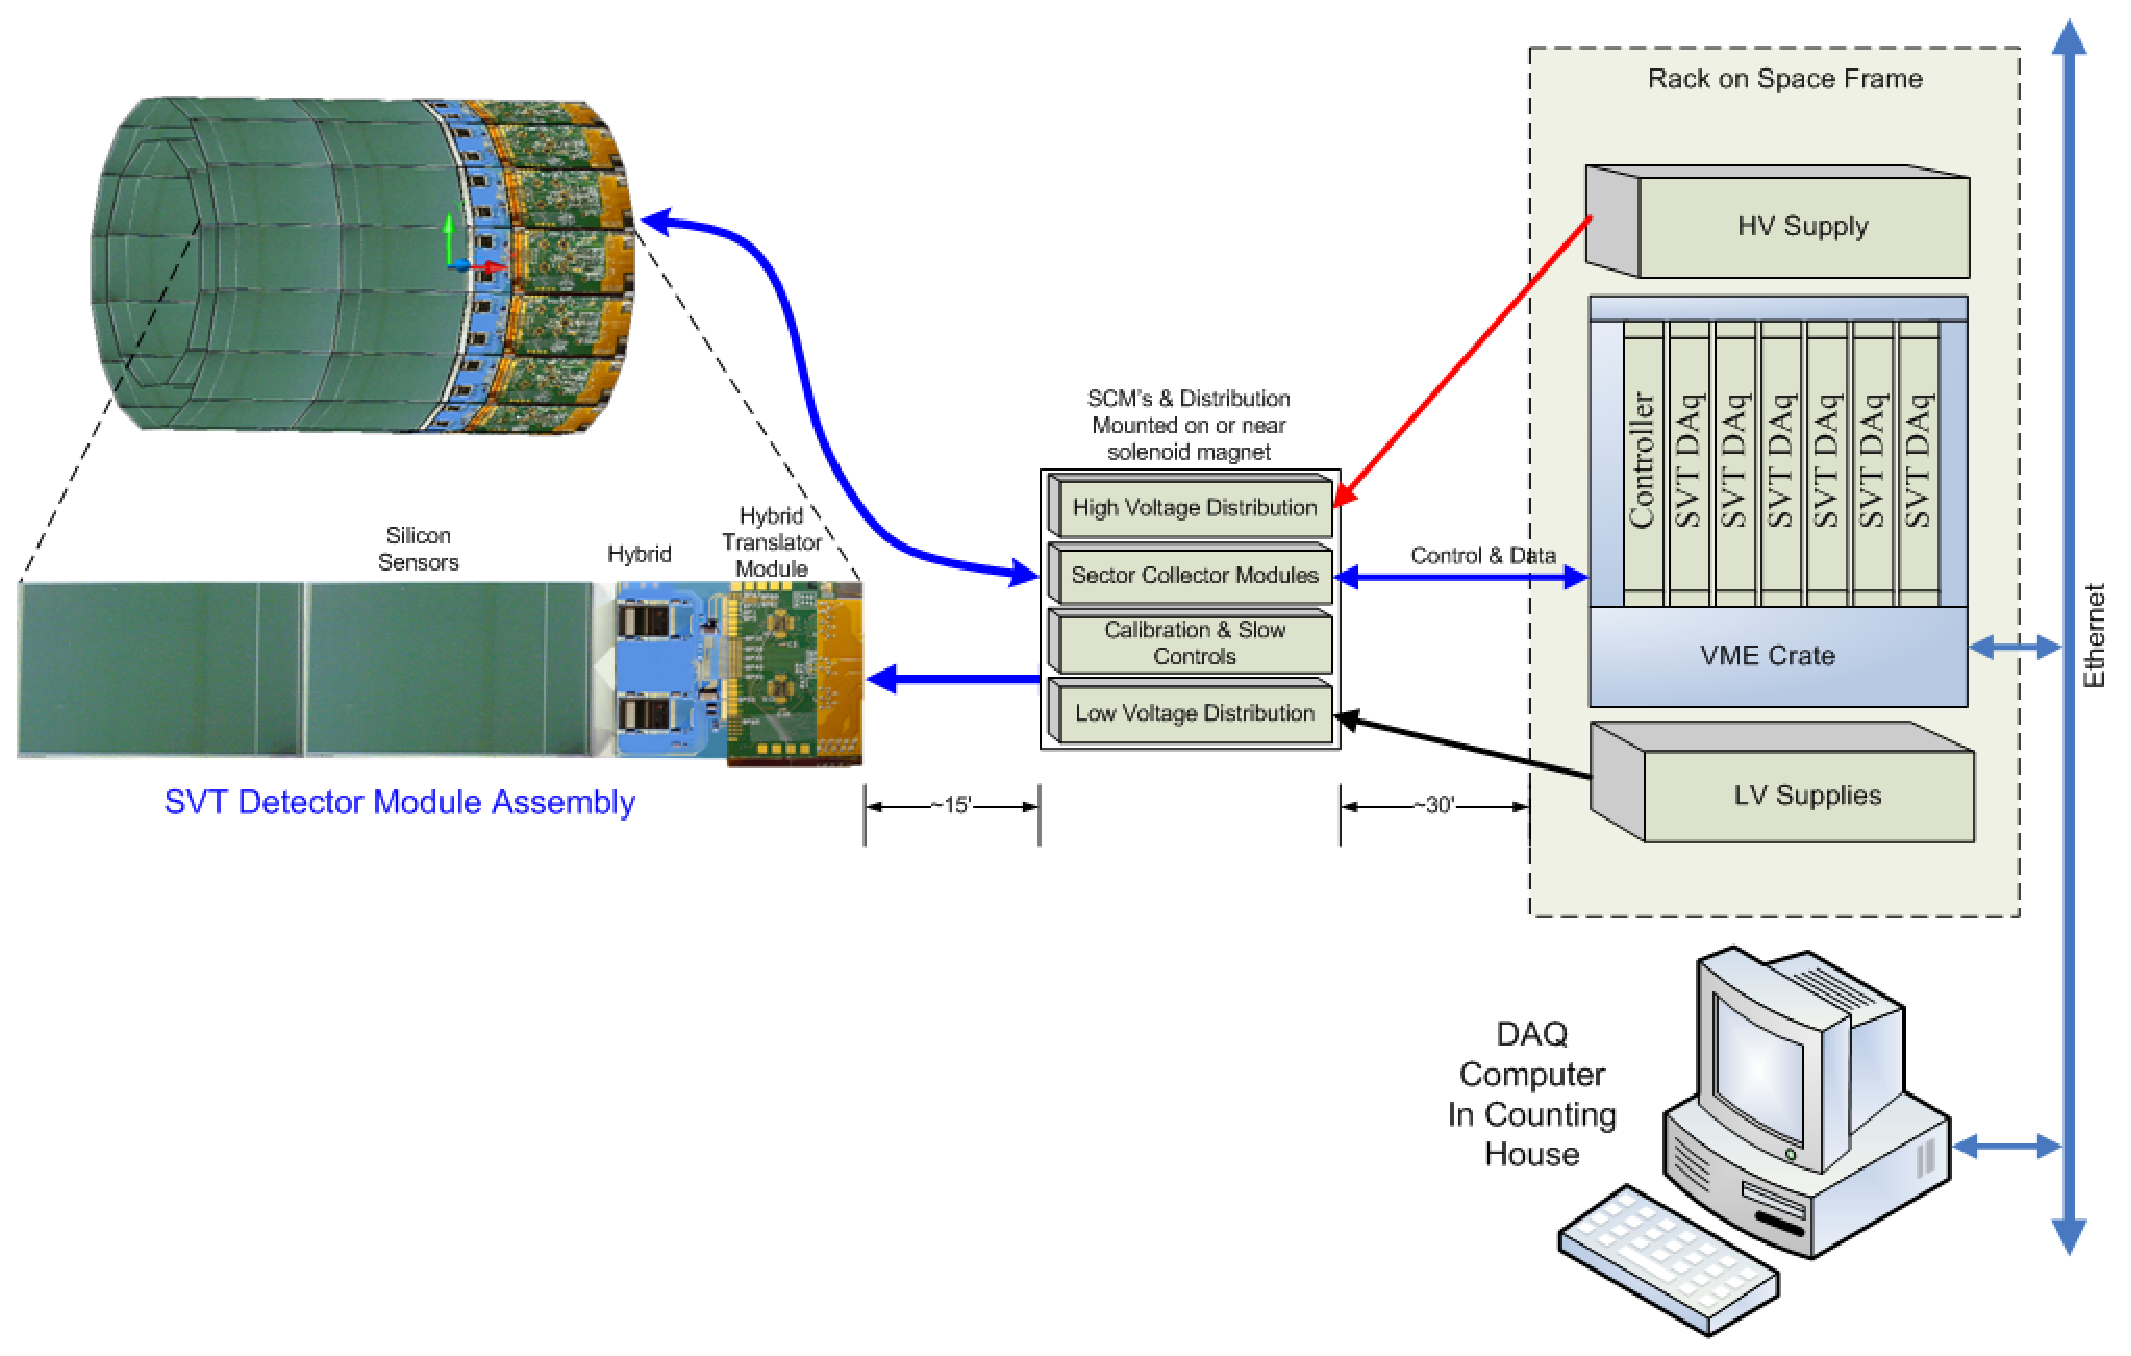
\includegraphics[width=0.9\textwidth]{system-connections}
\caption{\small{System connections overview for the SVT.}}
\label{fig:system-connections}
\end{figure}
%%%%%%%%%%%%%%%%%%%%%%%%%%%%%%%%%%%%%%%%%%%%%%%%%%%%%%%%%%%%%%%%%%%%%%%

\subsection{Slow Controls}

Calibration and testing of the detector modules and readout chain is 
accomplished by a calibration input signal (VCAL).  This external input 
on each SVX4 ASIC has the capability of injecting a small charge via a  
charge injection capacitor (25~fF).  This capacitor can be switched in 
from each preamp input to a common bus line.  A 128-bit programmable 
channel register, downloaded in the initialize mode, can function as a 
mask register and determine whether or not the injection capacitor is 
switched on for each channel.  Fig.~\ref{fig:svx-block} (left) shows the 
preamp stage of the SVX4 ASIC and the VCAL calibration input.

The slow controls system (SCS) will be responsible for controlling all 
essential run-time parameters of the experiment and for monitoring the 
status of various hardware components.  The primary goals are to enhance 
safety by providing early warnings about malfunctioning equipment and check 
the health of the experiment and the integrity of data.  The system will 
also transmit important parameters to the DAQ for insertion in the 
{\tt CLAS12} data stream.  The SCS will have the ability to trigger alarms 
to notify personnel when parameters are detected to be outside pre-defined 
limits and will have the option of automatically disabling DAQ in case of 
a severe malfunction of the equipment.  The implementation of the SCS will 
need a VME crate with an IOC and input/output boards.  Some of the hardware 
will be connected directly to the Ethernet network.  The settings of all 
critical operating parameters will be protected against computer failure.  
The failure of the computer in the system will only result in the loss of 
monitoring.  When a computer reboots, parameters will not reset to 
previous or default values but remain at currently set values.

The SVT computers and vital support hardware will be protected by 
Uninterruptible Power Supplies (UPS) with battery backup and software to 
signal an alarm and notify the operators when external power is lost.
The UPS will have surge protection and line filtering.  Monitoring and 
control of the system will be implemented through the use of a Motorola 
single board computer embedded in a VME crate running VXworks real-time 
operating system.  Sun or Hewlett-Packard workstations will support the 
user interfaces and controls.  The control software will be built using 
the toolkit provided by the Experimental Physics and Industrial Control 
System (EPICS), which is based on the client-server model.

\subsection{Data Acquisition}
\label{svt:daq}

Each channel of the SVX4 ASIC has a 42-cell deep analog pipeline.
Fig.~\ref{fig:svx-block} shows the block diagram of the ASIC.  The 
front-end of the ASIC contains the integrator and storage pipeline, which 
at a front end clock rate (FEClk) of 132~ns, allows a trigger latency of 
$\sim$4~$\mu$s.  The back-end of the ASIC has an ADC for digitization and 
the readout and driver logic.

%%%%%%%%%%%%%%%%%%%%%%%%%%%%%%%%%%%%%%%%%%%%%%%%%%%%%%%%%%%%%%%%%%%%%%%
\begin{figure}[htbp] 
\centering
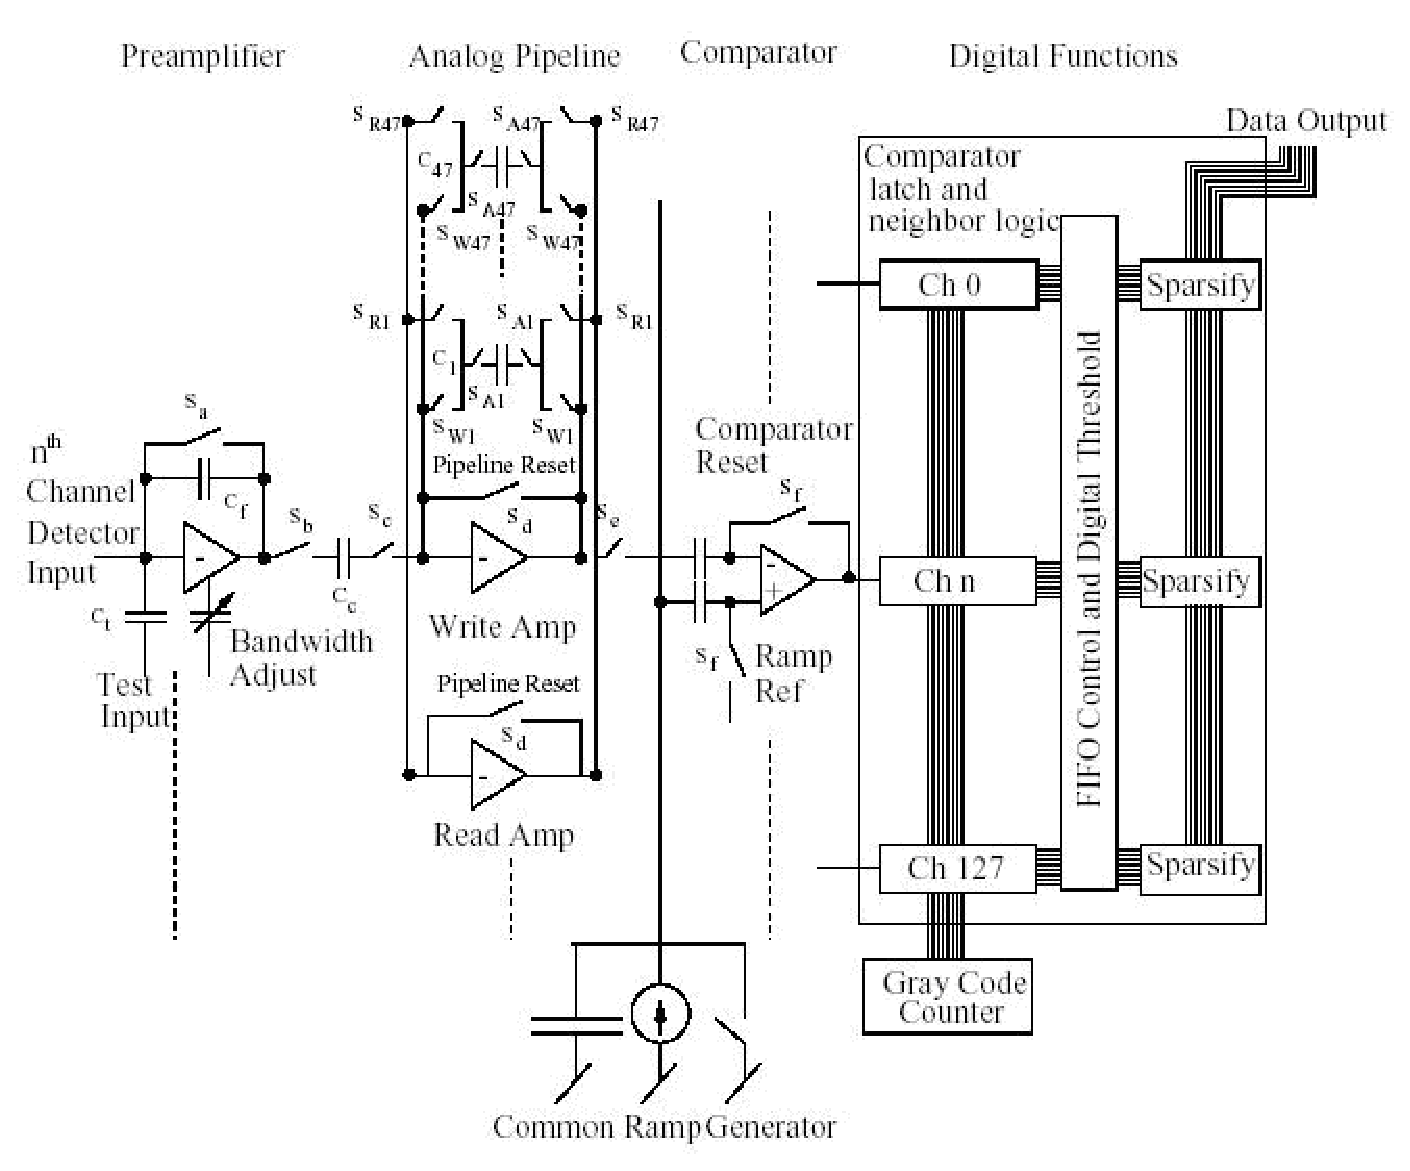
\includegraphics[width=0.75\textwidth]{svx-block}
\caption{\small{Block diagram of the SVX4.}}
\label{fig:svx-block}
\end{figure}
%%%%%%%%%%%%%%%%%%%%%%%%%%%%%%%%%%%%%%%%%%%%%%%%%%%%%%%%%%%%%%%%%%%%%%%

The Level-1 accept (L1A) signal to the ASIC is used to remove a ``hit'' 
cell from the pipeline.  The hit is temporarily stored in a FIFO buffer 
that can store up to four cells, corresponding to four L1As.  These hits 
are queued for readout to the back-end.  Once four cells are stored in 
the FIFO, additional L1As are ignored.  The trigger latency is programmed 
in the shift register during the initialize mode so that the right pipeline 
cell is read out.  L1A is normally high during acquisition and pulsed low 
to store a cell.  L1A must go low and return high between front-end clocks.  

The pedestal pipeline cell is reserved for acquiring only pedestal data.  
This cell is used during readout along with a stored cell.  The back-end 
digitizes the difference between the hit cell and the pedestal cell.  The 
pedestal cell is not part of the round robin ensemble of acquisition cells, 
hence the pedestal cell must be refreshed periodically.  Because of the 
continuous electron beam, L1A arrivals are not synchronized to the 
front-end clock, which implies that the associated detector signals are 
Poisson-distributed with respect to this clock.

SVX4 data acquisition rates at a luminosity of 
$1\times10^{35}$~cm$^{-2}$s$^{-1}$ were simulated to check their performance 
in a continuous electron beam environment.  The first aspect of the SVX4 
that was simulated was the L1A acceptance rate~\cite{CN2006-13}.  The 
triggers generated were Poisson-distributed with respect to the SVX4s FEClk.  
The simulation estimated the number of triggers that had an early arrival 
time and also estimated the number of triggers that were missed.  The results 
of the simulation showed that for half-field operation of the solenoid, 2.5~T, 
with an L1A rate of 10~kHz, $\sim$0.1\% of the triggers arrived early.  No 
triggers were missed.  The simulation was run for an L1A rate of 100~kHz as 
well, over ten times the expected trigger rate.  For these conditions only 
$\sim$1.3\% of the triggers arrived early and $\sim$0.3\% triggers were 
missed.

Another simulation checked the effect of issuing a reset and the associated 
restore operation when the pre-amplifiers on the chip saturate
\cite{CN2006-24}.  In operating the SVX4, charge is accumulated on the 
pre-amplifier and this charge needs to be periodically reset when it reaches 
$\sim$200~fC.  The results of these simulations show that at half-field of
the solenoid, a $\sim$1\% deadtime can be expected; at full-field operation 
the deadtime is $\sim$0.4\%.

SVX4 is designed for daisy-chained operation.  Daisy-chaining minimizes 
the number of bus and control lines required to operate the device.  Fewer 
control lines means less space on the high density interconnect and less 
mass in the system.  All the chips share a common communication bus and a 
common differential and back-end clock.  Each chip has two pads that are 
used for communication between adjoining chips.  After powering up the SVX4, 
the chip parameters must be downloaded before operation of the readout chips 
can begin.  For each SVX4 chip, 198 bits must be downloaded into the 
internal registers.

%%%%%%%%%%%%%%%%%%%%%%%%%%%%%%%%%%%%%%%%%%%%%%%%%%%%%%%%%%%%%%%%%%%%%%%
\begin{figure}[htbp]
\centering
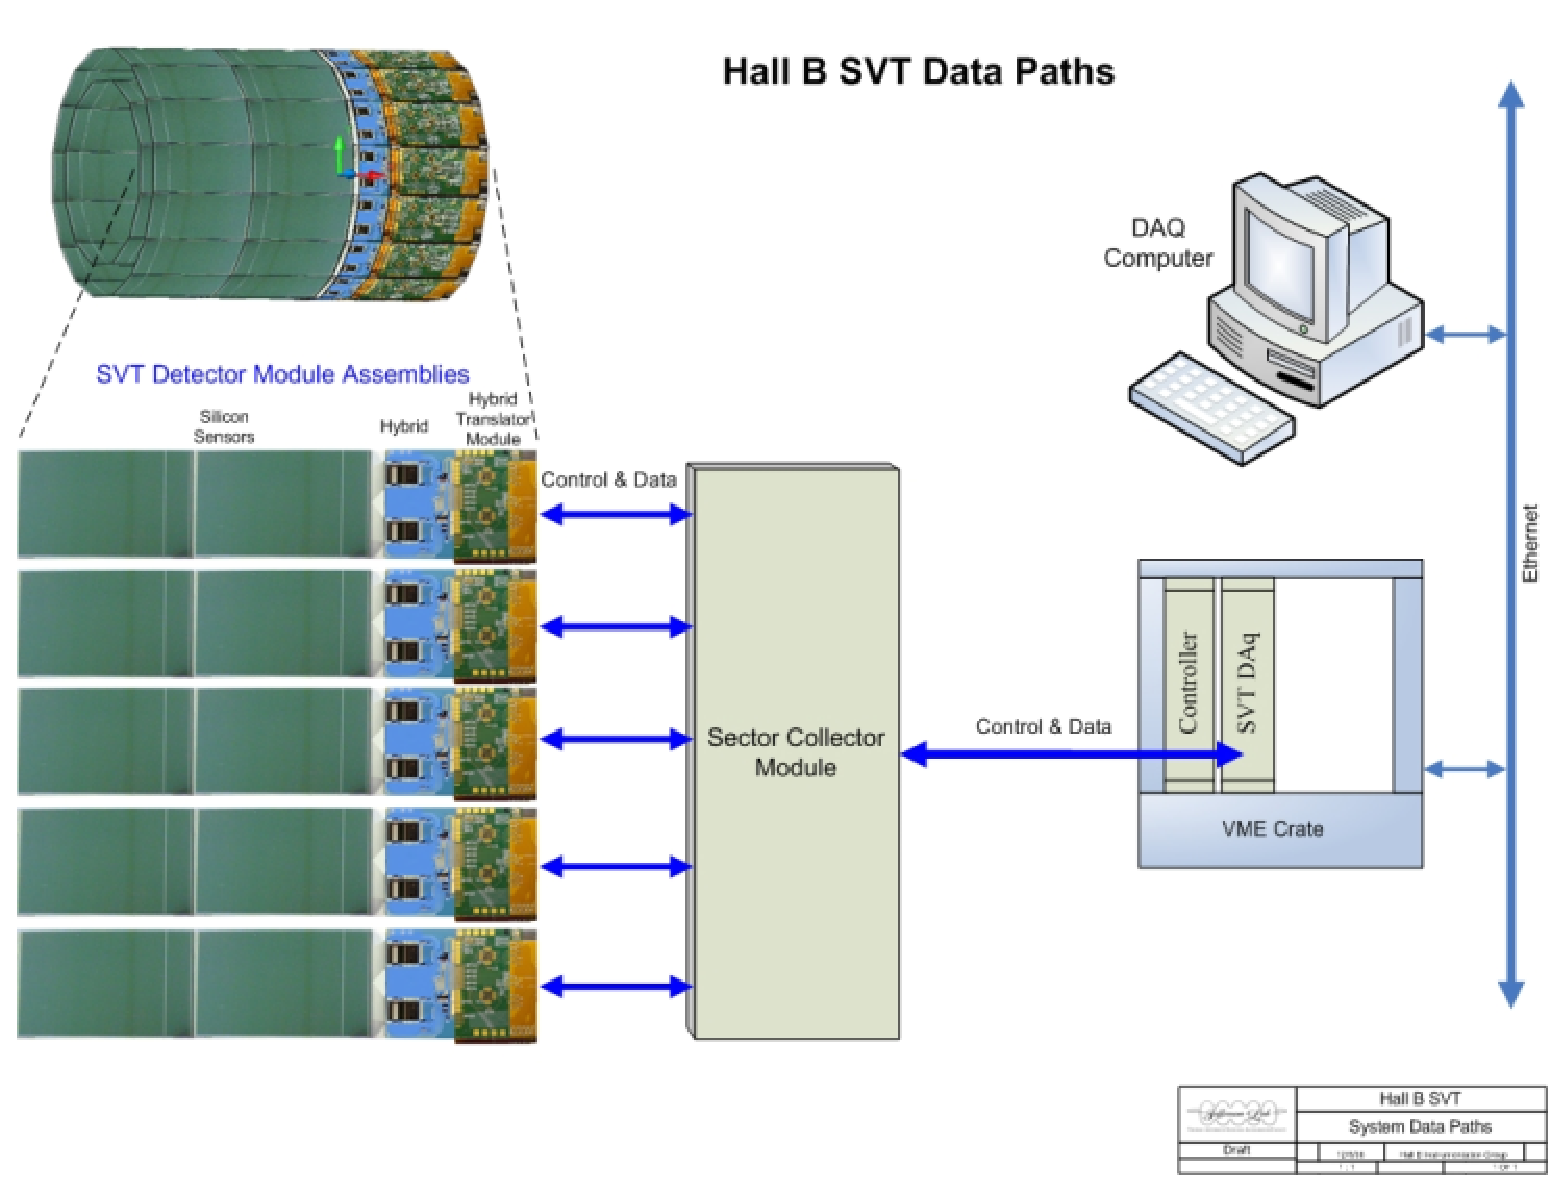
\includegraphics[width=0.70\textwidth]{data-path}
\caption{\small{SVT system data paths.}}
\label{fig:data-path}
\end{figure}
%%%%%%%%%%%%%%%%%%%%%%%%%%%%%%%%%%%%%%%%%%%%%%%%%%%%%%%%%%%%%%%%%%%%%%%

Fig.~\ref{fig:data-path} shows the data path for the Hall B SVT system.
Signals are digitized in the SVX4 ASICs on the hybrids.  The control 
signals and data bus for a module are connected to a sector collector
module (SCM).  Up to five modules are connected to an SCM that buffers 
and passes the data and control signals to the DAQ system.  SCMs may also 
be daisy-chained together to form a longer readout chain.  The readout 
chain requires only one detector module buffered by a single SCM to form 
a valid control and data path.  Unused SCM inputs are bypassed.  Increasing 
the number of SCMs connected together increases the daisy-chain length and 
the DAQ readout time.  The fastest readout is accomplished by a single 
silicon detector module, SCM, and SVT DAQ module chain.  
Fig.~\ref{fig:scm-daisy-chain} shows the daisy chain connections through 
an SCM.

%%%%%%%%%%%%%%%%%%%%%%%%%%%%%%%%%%%%%%%%%%%%%%%%%%%%%%%%%%%%%%%%%%%%%%%
\begin{figure}[htbp]
\centering
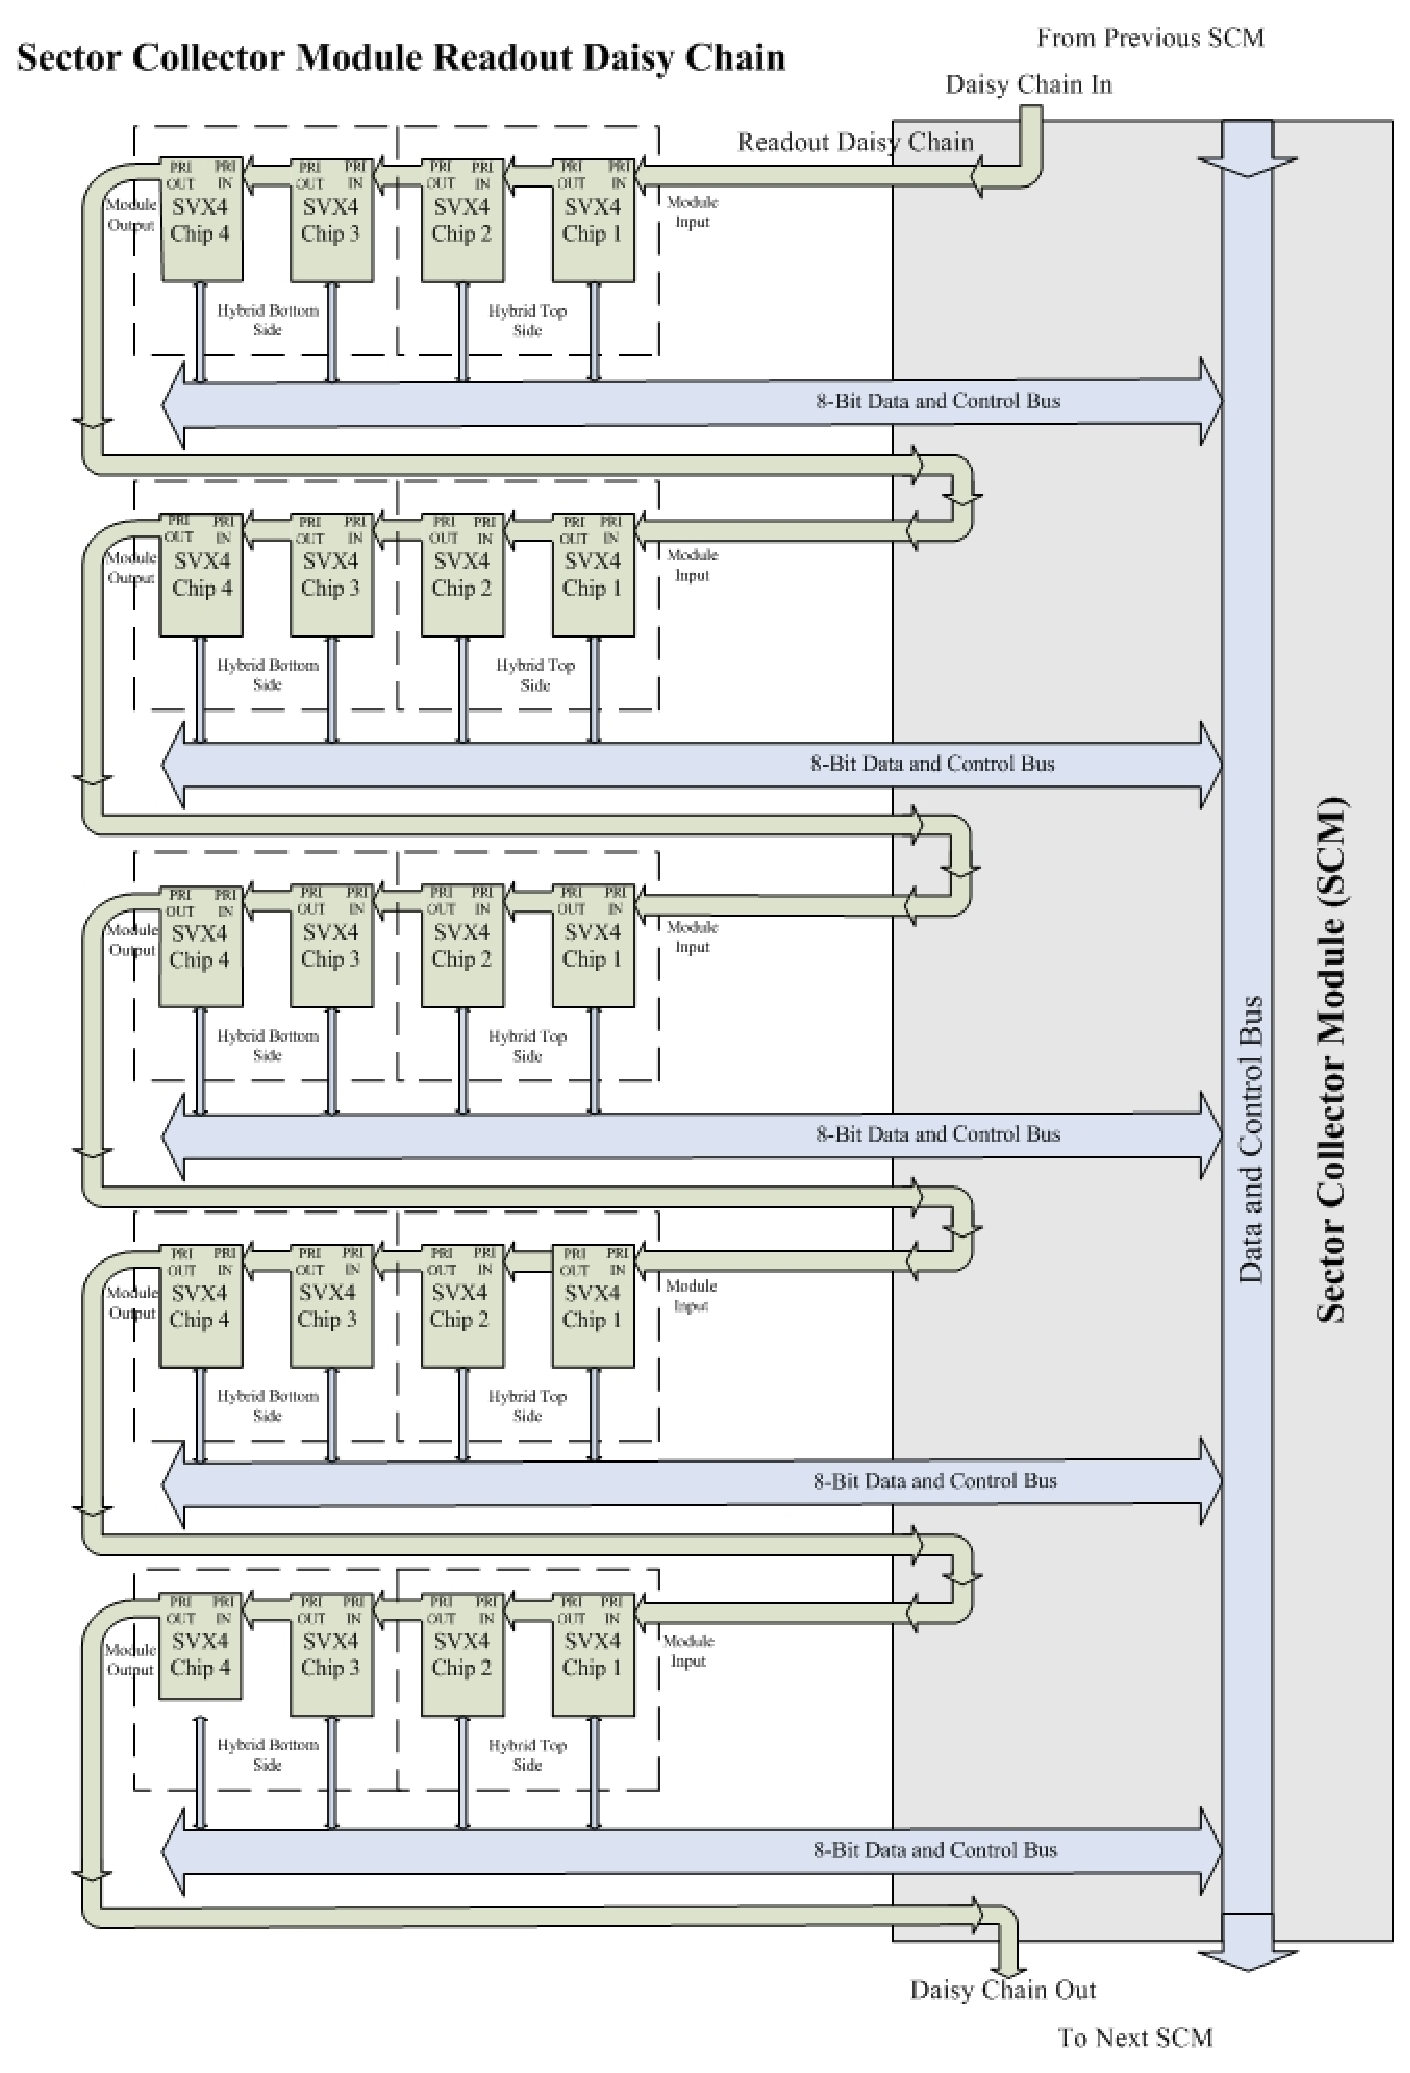
\includegraphics[width=0.6\textwidth]{scm-daisy-chain}
\caption{\small{Sector collector module daisy-chain readout.}}
\label{fig:scm-daisy-chain}
\end{figure}
%%%%%%%%%%%%%%%%%%%%%%%%%%%%%%%%%%%%%%%%%%%%%%%%%%%%%%%%%%%%%%%%%%%%%%%

For the {\tt CLAS} upgrade, VME systems will be used for both DAQ and slow 
controls.  Currently, {\tt CLAS} uses about 30 VME crates and several types 
of modules.  As a standard DAQ framework at JLab, 6U VME single board 
computers (SBCs) running VxWorks RTOS are used.  The Harvard-designed 
Silicon Readout Controller (SRC) used in FNAL-CDF was studied for possible 
implementation in our system.  This controller was originally designed for 
SVX3 readout.  The CDF-SRC printed circuit board is in 9U VME format.  This 
format is incompatible with our 6U-sized systems.  The board has nine FPGAs 
and only controls the SVX3 ASIC.  Separate VME hardware is needed to handle 
and store the data received from the silicon sensors.  In addition, this 
SRC is application specific for the pulsed accelerator at FNAL and designed 
around the triggering system used at CDF.

For control and data acquisition for the SVT, a 6U VME board compatible 
with the {\tt CLAS} data stream format is being developed~\cite{CN2004-04}.
This modular SRC will control and integrate the data received from the SVT 
readout chain into the DAQ system.  Fig.~\ref{fig:src-block} shows the block 
diagram of the prototype SRC.  The heart of the SRC design is 
Field-Programmable Gate Arrays (FPGAs).  The advantage of FPGA technology 
is that it combines the ease of software with the speed of hardware with 
permanent upgrade capabilities via downloaded updates.  FPGAs have already 
provided the lab with versatile VME bus data acquisition and control 
interfaces.  Current JLab FPGA designs provide control and monitoring for 
numerous systems by interfacing sensors and instrumentation with ADCs and
TDCs.  As shown in Fig.~\ref{fig:src-block}, data and control signals from 
the readout chain connect to the SVX4 controller FPGA logic for processing.  
Interface I/O signals are provided by the FPGA for external triggering, 
clock, and phase lock interfaces among others.  The FPGA has a memory 
management unit and PCI interface that connects to the VME interface.  
On-board memory stores the events to be read out.  The VME slave interface 
completes the data and control path to the VME backplane through bus 
transceivers.

%%%%%%%%%%%%%%%%%%%%%%%%%%%%%%%%%%%%%%%%%%%%%%%%%%%%%%%%%%%%%%%%%%%%%%%
\begin{figure}[htbp]
\centering
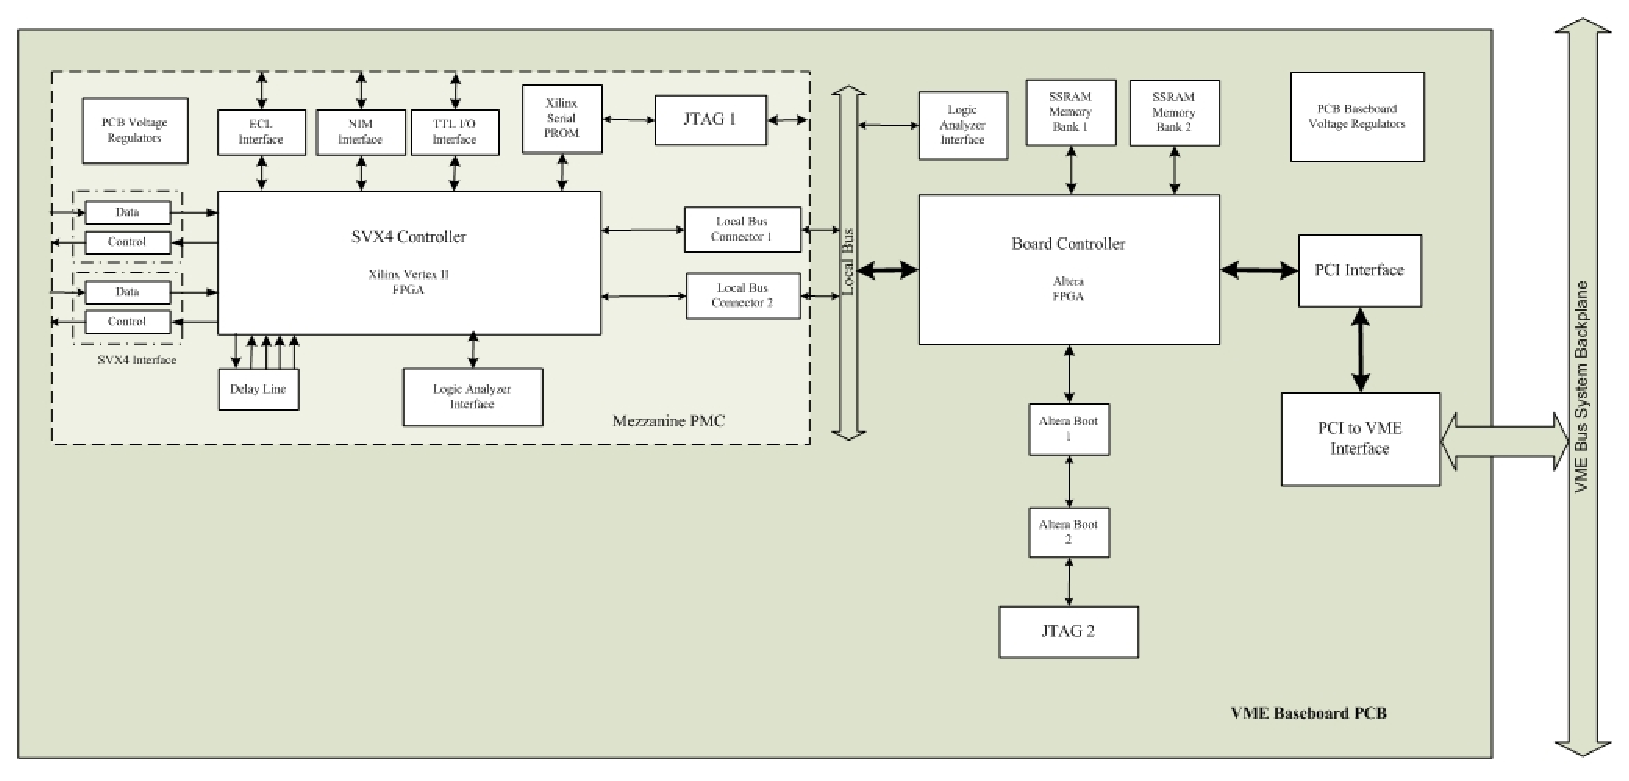
\includegraphics[width=0.7\textwidth]{src-block}
\caption{\small{SRC prototype block diagram.}}
\label{fig:src-block}
\end{figure}
%%%%%%%%%%%%%%%%%%%%%%%%%%%%%%%%%%%%%%%%%%%%%%%%%%%%%%%%%%%%%%%%%%%%%%%

The SRC generates initialize, acquisition, digitization, and readout 
timing sequences for the SVX4 ASIC.  The initialization cycle is typically 
performed once, followed by repetitive data acquisition, digitization, and 
readout sequences.  Since we will be operating the SVX4 ASIC in 
continuous data format mode, the acquisition cycle occurs simultaneously 
with the digitize and readout sequences.  After the hit cell has been 
digitized in the SVX4, the SRC starts a readout cycle and the event data 
is stored locally.  The event data will be continuously stored until the 
SRC is instructed to read out the data by the VME system controller or 
until the local memory is full.  The VME slave interface on the SRC accepts 
instructions from the VME SBC.  These instructions control the SVX4 
sequences and read out the stored events.  The SRC status register reports 
on the operating condition of the board including memory overflow.

The SRC design includes a Joint Test Action Group (JTAG) interface that 
provides In System Programming (ISP) capability.  The ability to reprogram 
the on-board components provides a permanent upgrade path via software 
updates.  It also provides a way to implement new features (even remotely) 
into an existing system after fabrication and installation.  In addition, 
JTAG technology can be used for board level interconnection and 
functionality testing.

Based on the GEANT3 simulation, approximately 16 particles will be 
generated per trigger in the cone part of the SVT when the solenoid is 
operating at half-field.  The forward cone is split into four groups, 
three of which have six modules and the last group has four modules.  The 
four group partition results in four tracks per group per trigger.  Six 
modules have 24 ASICs in all.  For each chip, the pipeline cell and ID has 
to be read; this contributes 96 bytes, whether or not there is data.  Four 
tracks in a group give rise to 6 hits, each of which requires a byte for 
cell ID and a byte for content, contributing 12 bytes per track.  Therefore 
there are 48 bytes per track from hits alone.  Therefore, there are 144 
bytes per trigger.  Since the groups are independently read out, this data 
rate translates to 1.44~MB/s for a trigger rate of 10~kHz, well below the 
56~MB/s readout rate capable by the ASIC.  Our expectations for the time 
taken for digitization and readout as a function of the number of hits in 
a sector of the FST have been computed and are shown in Fig.~\ref{readtiming}.
Each sector can handle up to 2500 hits in 105~ns (25~MHz).  A higher rate 
implies that before the digitization process can be completed a new L1A 
arrives, eventually filling up the FIFO and leading to a loss of triggers.

%%%%%%%%%%%%%%%%%%%%%%%%%%%%%%%%%%%%%%%%%%%%%%%%%%%%%%%%%%%%%%%%%%%%%%%
\begin{figure}[htbp]
\centering
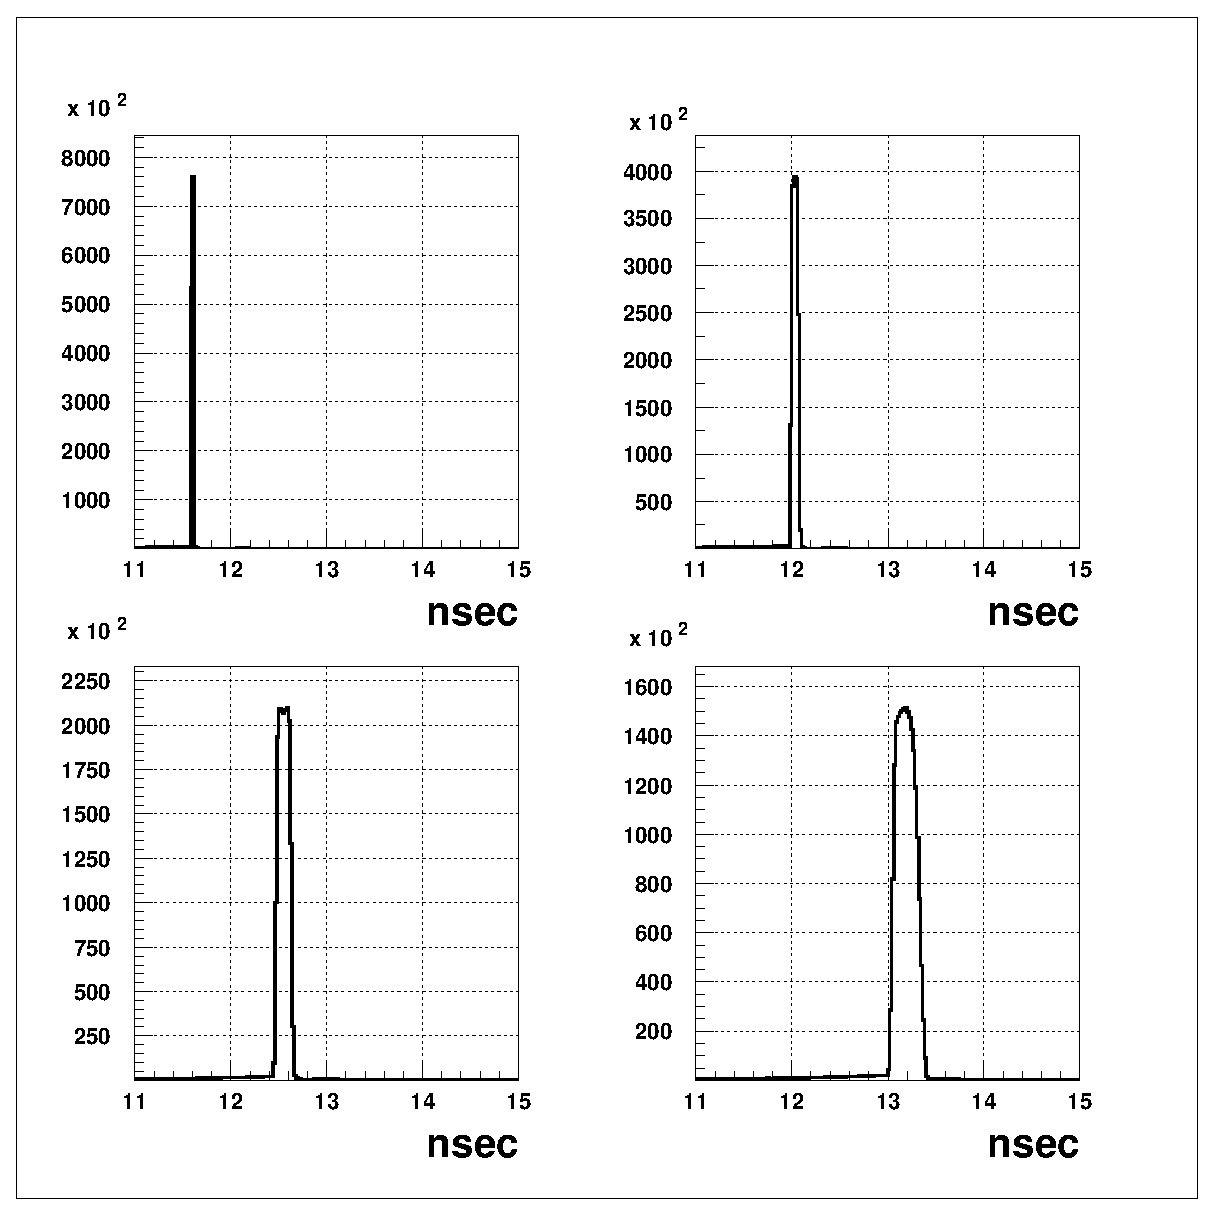
\includegraphics[width=0.8\textwidth]{timing}
\caption{\small{Readout time as a function of the number of hits in a
given layer or portion of the SVT.}}
\label{readtiming}
\end{figure}
%%%%%%%%%%%%%%%%%%%%%%%%%%%%%%%%%%%%%%%%%%%%%%%%%%%%%%%%%%%%%%%%%%%%%%%

\section{Research \& Development}

R\&D for the SVT system started in FY2004~\cite{CN2004-29}.  The R\&D 
goals are to evaluate silicon strip detector systems, assess compatibility 
of SVX4 performance with {\tt CLAS12} requirements, study the features of 
the FNAL stave design that could be useful for {\tt CLAS12}, and gain 
experience and know-how about developing support fixtures, installation, 
and DAQ by conducting lab tests and installing a test stave in Hall B for
in-beam tests~\cite{CN2004-42}.  

The initial R\&D effort~\cite{CN2005-009,CN2005-016} focused on the DAQ 
system of the stave received from FNAL.  The Hall B Instrumentation 
Group modified the DAQ hardware and software to run lab and beam tests.  
Some of the significant modifications that were made were the addition of 
plots to show the number of hits in each strip, the archiving of selected 
real-time strip plots, the storage of output data for off-line analysis, 
the ability to change the clock-base, and the addition of the external 
trigger mode.  For the operation of the stave, low and high voltage control 
programs were researched, developed, and implemented
\cite{CN2005-017,CN2005-018}.  

R\&D activities during FY2004 culminated with the conduction of beam tests
\cite{CN2005-020}.  To perform these tests, specialty cables, data 
buffers, data repeaters, controls and monitoring programs for low and high 
voltages, DAQ software, off-line analysis software, support structures, and 
finite element analyses were designed, developed, debugged, and implemented.  
The significant result of the FY2004 R\&D effort was that it provided 
hands-on experience with several facets of the endeavor to build a reliable 
state-of-the-art silicon vertex tracker tailored to meet {\tt CLAS12} 
requirements.  For FY2005 the R\&D plan was to develop a laser test stand 
and a PCI-based DAQ board~\cite{CN2005-019}.  However, due to budgetary 
considerations, work was done only on the laser test stand.  Additionally,
the prototype FPGA-based, PCI-bus-compatible, printed circuit carrier board 
for the DAQ controller of the SVT was successfully built and tested
\cite{CN2006-010} (see Fig.~\ref{fig:marc1}). 

%%%%%%%%%%%%%%%%%%%%%%%%%%%%%%%%%%%%%%%%%%%%%%%%%%%%%%%%%%%%%%%%%%%%%%%
\begin{figure}[htbp]
\centering
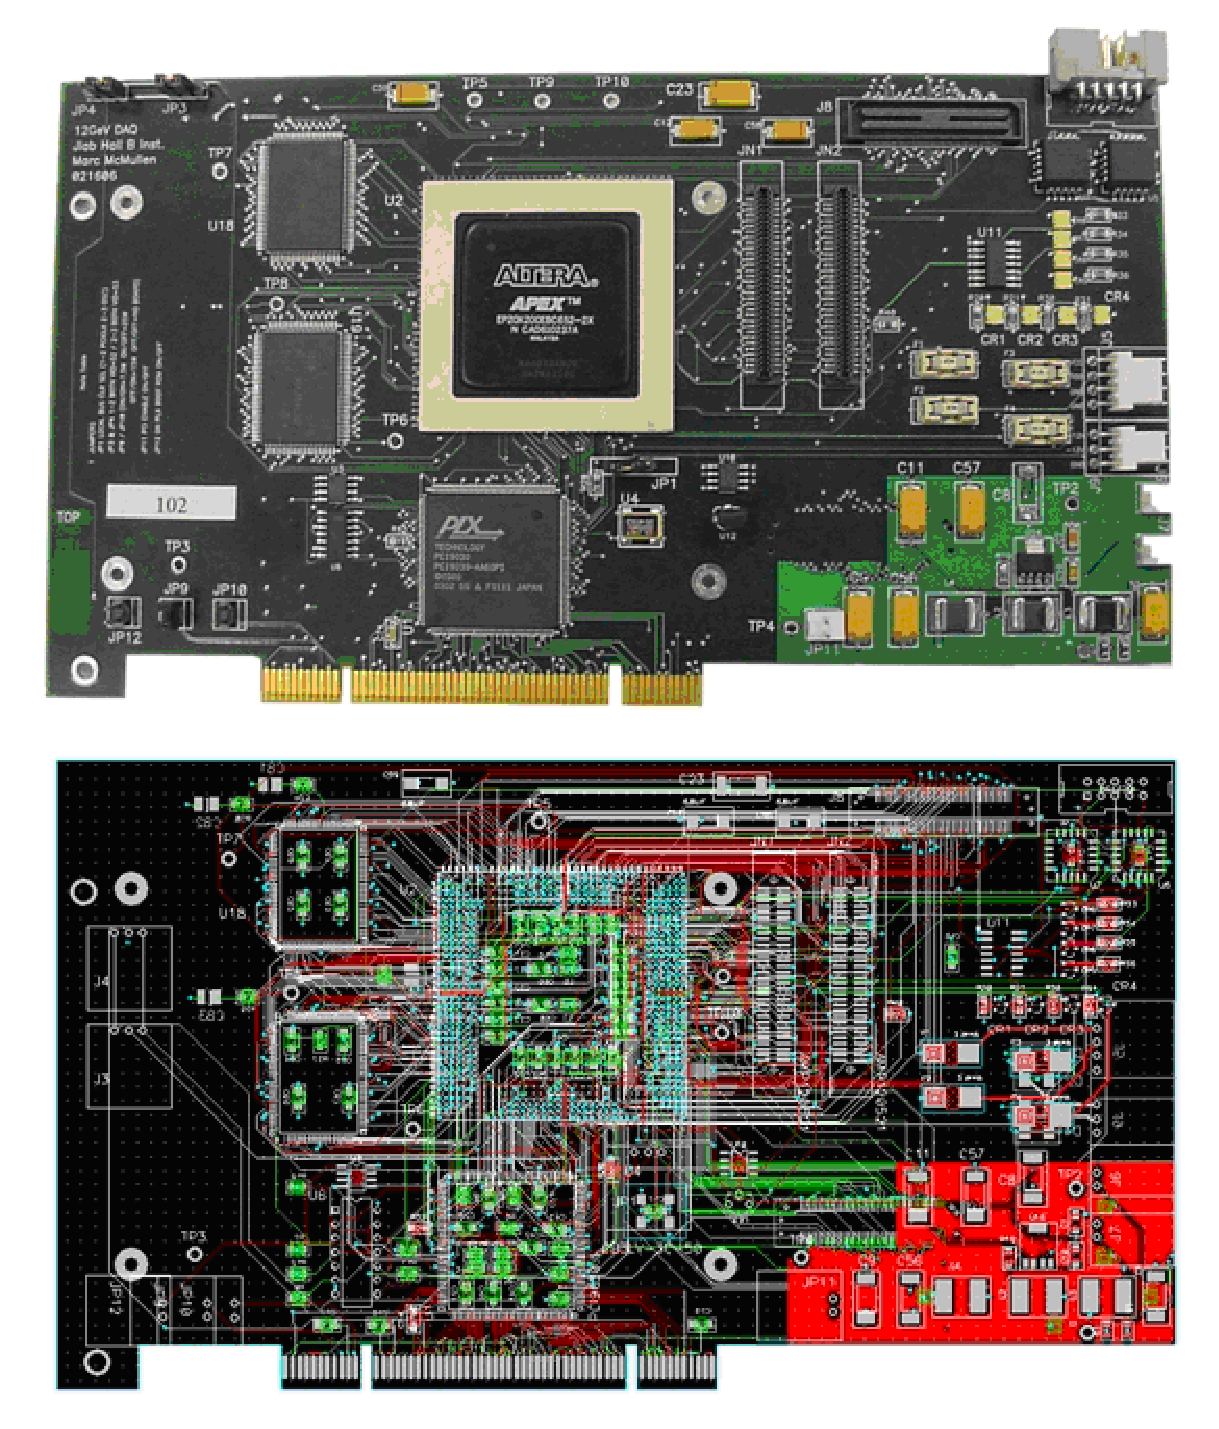
\includegraphics[width=0.45\textwidth]{marc1}
\caption{\small{New PCI-based {\tt CLAS12} DAQ base board.}}
\label{fig:marc1}
\end{figure}
%%%%%%%%%%%%%%%%%%%%%%%%%%%%%%%%%%%%%%%%%%%%%%%%%%%%%%%%%%%%%%%%%%%%%%%

%%%%%%%%%%%%%%%%%%%%%%%%%%%%%%%%%%%%%%%%%%%%%%%%%%%%%%%%%%%%%%%%%%%%%%%
\begin{figure}[htbp]
\centering
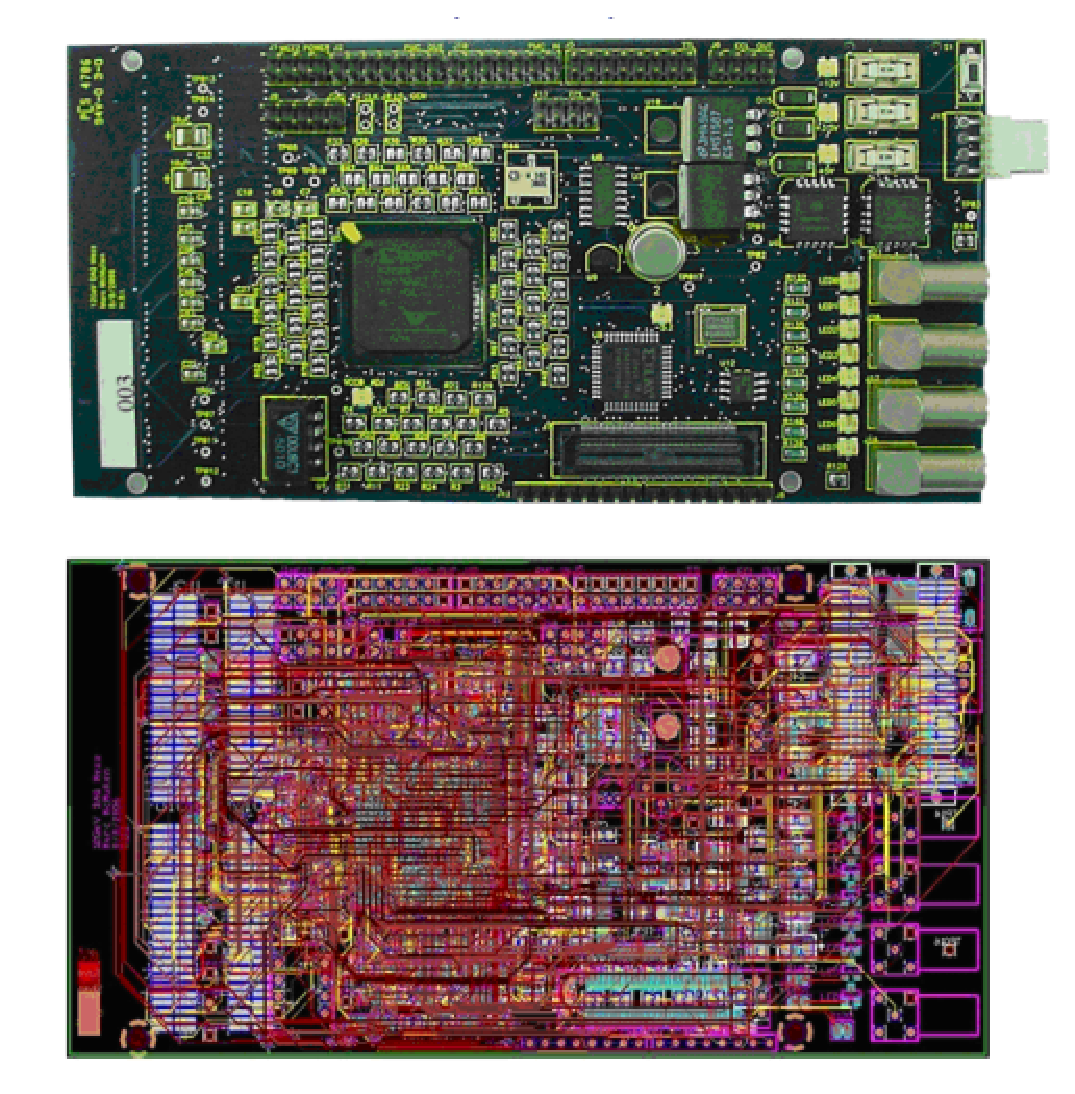
\includegraphics[width=0.5\textwidth]{marc2}
\caption{\small{SVX4-based PMC controller card.}}
\label{fig:marc2}
\end{figure}
%%%%%%%%%%%%%%%%%%%%%%%%%%%%%%%%%%%%%%%%%%%%%%%%%%%%%%%%%%%%%%%%%%%%%%%

R\&D for FY2006 focused on the design of the DAQ mezzanine circuit board
(shown in Fig.~\ref{fig:marc2}) that will be compatible with a VME board.  
The block diagram for the circuit board is shown in 
Fig.~\ref{fig:daq-pcb-block}.  The FPGA design of the SVT DAQ/controller 
board is flexible and permits use of different silicon sensor readout ASICs.

%%%%%%%%%%%%%%%%%%%%%%%%%%%%%%%%%%%%%%%%%%%%%%%%%%%%%%%%%%%%%%%%%%%%%%%
\begin{figure}[htbp]
\centering
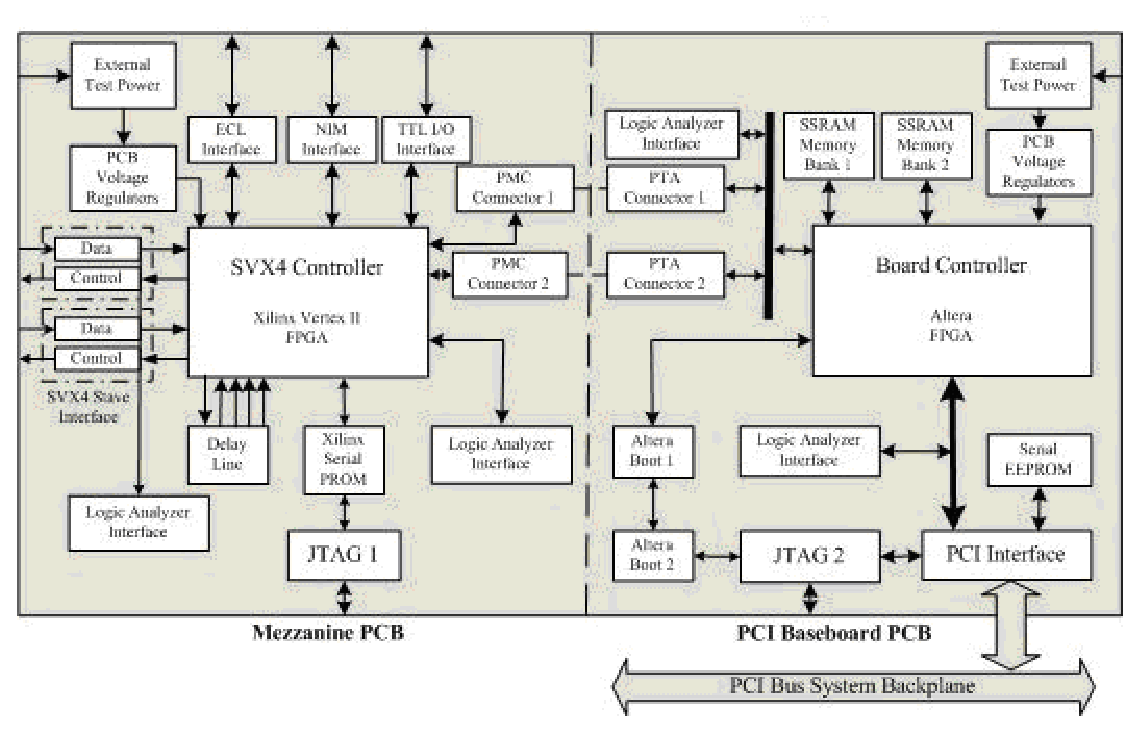
\includegraphics[width=0.75\textwidth]{daq-pcb-block}
\caption{\small{Prototype DAQ circuit board diagram.}}
\label{fig:daq-pcb-block}
\end{figure}
%%%%%%%%%%%%%%%%%%%%%%%%%%%%%%%%%%%%%%%%%%%%%%%%%%%%%%%%%%%%%%%%%%%%%%%

R\&D on the advanced conceptual design for the SVT is continuing.  Support 
structures and instrumentation strategies are being developed, and detector 
installation procedures are being studied.  Safety issues for each step of 
the detector construction and installation are being analyzed.

\section{SVT Commissioning and Operation}

The objective of the SVT commissioning plan is to debug, fix, and
calibrate system components.  Over the last several decades, much
experience in this area has been gathered by experiments at other
facilities.  The SVT commissioning program will draw on these experiences.
The commissioning plan includes studies without and with beam.

After installation of the SVT in the solenoid, a complete set of system
checks will be performed.  First, a visual inspection of cables and
electronics will be carried out.  Control, data, low voltage (LV), high
voltage (HV), and monitoring cables will be checked for proper strain relief,
sheathing, insulation integrity, and connections.

The detector will be monitored continuously by the {\tt CLAS12} slow controls
system.  The slow controls procedures to adjust critical parameters of the
equipment will be checked.  Power will not be turned on until all alarms and
fail-safe systems have been verified.  Power-up tests will be conducted first
on dummy loads.  This checkout will include all systems controlled by EPICS
as well.

Temperature and humidity conditions in and around the SVT will be monitored
continuously.  Also, light sensors inside the SVT will monitor the level of
light infiltration.

The LV system, including LV distributions, will be checked with dummy loads.
Correlations between demand, monitored, and measured voltages will be logged.
Once it is ascertained that the LV system is functional, it will be connected
to the SVT.  The HV system will be checked in a similar fashion.

Once both the LV and HV systems have been checked, the SVT will be powered
up; the power-up sequence will be, first the LV system, and then the HV
system.  The powering up of both the systems will be done in appropriate steps.
Current draw by both the systems will be automatically recorded.

Read/write tests on the ASIC registers will check whether all ASICs are able
to be programmed and whether they can be read back.  Calibration of the detector 
modules and testing of the readout chain will be accomplished by inputting an 
external signal.  This external input on each SVX4 ASIC has the capability of
injecting a small charge via a small charge injection capacitor (25~fF).  
Calibration will be done with different inject masks.  The acquired ADC spectra
will be used to calibrate the ASICs.  The performance of the system, including 
that of the front-end electronics, will be checked at the channel level by 
inspecting the occupancy plots.

Hit/no hit data will indicate noisy or dead channels.  An effort will be
made to fix channels with problems by appropriate measures, such as varying
the threshold, low, and high voltage values.

Once these basic tests have been completed, efficiency and tracking accuracy
tests will be performed using cosmic rays.  Cosmic triggers generated by the
CTOF will be used to measure the efficiency and the track reconstruction
accuracy in the Barrel Silicon Tracker.  These tests will be done for zero,
half, and full fields of the solenoid.  Tracks will be reconstructed in the
eight SVT layers in the upper hemisphere and the projected track hits will
be checked against the registered hits in the eight layers of the opposite
hemisphere.  These tests will be repeated with test beam.

\section{{\tt CLAS12} Drift Chambers}

\subsection{Overview}

The overall tracking requirements (0.5 -  1\% fractional momentum resolution 
at 5~GeV and efficient tracking at a luminosity of 
10$^{35}$~cm$^{-2}$s$^{-1}$) are the main drivers for drift chamber design.  
Because the {\tt CLAS} drift chamber system~\cite{dcnim} has operated 
successfully for 8~years, we plan to re-use many of the design concepts and 
most of the utility infrastructure.  In particular, we plan to re-use the 
present gas mixing and handling system, the high-voltage and low-voltage 
systems, the FASTBUS TDC system, and the post-amplifier/multiplexer systems.
The construction project thus consists of new chambers, on-board electronics, 
and on-board jumper cables.

The forward tracking system consists of three regions divided into six
sectors as shown in Fig.~\ref{umbrella}; located just before, inside, 
and just outside the torus field volume, and referred to as Regions~1, 2, 
and 3.  Each chamber will have its wires arranged in two superlayers of
six layers each, with the wires in the two superlayers strung with 
$\pm$6$^\circ$ stereo angles, respectively.  The cell structure will be 
hexagonal, that is, each sense wire is surrounded by six field wires.  This 
arrangement is similar to the present {\tt CLAS} design and offers good 
resolution with very good pattern recognition properties.  Refer to our 
article on the overall {\tt CLAS} detector~\cite{clasnim} and our article 
on the drift chambers themselves~\cite{dcnim} for details of the present 
detector and chambers.  The groups responsible for the {\tt CLAS12} drift
chamber construction include Old Dominion University, Idaho State
University, and Jefferson Laboratory.

%%%%%%%%%%%%%%%%%%%%%%%%%%%%%%%%%%%%%%%%%%%%%%%%%%%%%%%%%%%%%%%%%%%%%%%%
\begin{figure}[htbp]
\vspace{10.6cm}
\special{psfile=umbrella.ps hscale=60 vscale=60 hoffset=60 voffset=0}
\caption{\small{Schematic layout of the {\tt CLAS12} Forward Drift Chambers: 
Regions~1, 2, and 3.}}
\label{umbrella}
\end{figure}
%%%%%%%%%%%%%%%%%%%%%%%%%%%%%%%%%%%%%%%%%%%%%%%%%%%%%%%%%%%%%%%%%%%%%%%%

The major difference in the drift chambers for {\tt CLAS12} is that the 
cells cover a smaller solid angle than those in the present {\tt CLAS} 
chambers, allowing efficient tracking at higher luminosities because the 
accidental occupancy from particles not associated with the event is smaller.  
Table~\ref{fwd-dc-design-parms} lists the main design parameters for each 
region of the {\tt CLAS12} drift chambers.  For the purposes of simulating 
track resolutions, we assumed that the position resolution of the individual 
drift cells would be 250~$\mu$m.  

%%%%%%%%%%%%%%%%%%%%%%%%%%%%%%%%%%%%%%%%%%%%%%%%%%%%%%%%%%%%%%%%%%%%%%%%%
\begin{table}[ht]
\begin{center}
\begin{tabular} {||c|c|c|c||} \hline \hline
                     &{\bf Region 1}&{\bf Region 2}&{\bf Region 3}\\ \hline
Distance from target & 2.3 m    & 3.5 m        & 4.7 m    \\ \hline
Num. of superlayers  & 2        & 2            & 2        \\ \hline
Layers/superlayer    & 6        & 6            & 6        \\ \hline
Wires/layer          & 112      & 112          & 112      \\ \hline
Cell size            & 0.75 cm  & 1.18 cm      & 2.07 cm  \\ \hline
Active time window   & 150 ns   & 250 - 500 ns & 500 ns   \\ \hline
Resolution per wire  & 0.020 cm & 0.025 cm     & 0.030 cm \\ \hline
\end{tabular}
\caption{\small{Design parameters for the {\tt CLAS12} drift chambers.}}
\label{fwd-dc-design-parms}
\end{center}
\end{table}
%%%%%%%%%%%%%%%%%%%%%%%%%%%%%%%%%%%%%%%%%%%%%%%%%%%%%%%%%%%%%%%%%%%%%%%%%

There are also other differences in the design of the {\tt CLAS12} chambers 
compared to the current {\tt CLAS} chambers.  ways.  Successive superlayers 
have their wires arranged with a $\pm$6$^\circ$ stereo angle; the present 
arrangement has an axial layer and a 6$^\circ$ stereo layer.  For the present 
{\tt CLAS} detector, the $\phi$ resolution times $\sin \theta$ is about two 
times larger than the $\theta$ resolution.  To have more equal resolution in 
the two angles, we doubled our stereo angle from 0 and 6$^\circ$ to 
$\pm$6$^\circ$.  Unlike the present chambers, all of the wires in one of the 
superlayers are strictly parallel, and in a plane perpendicular to the wire 
direction, form perfect hexagons.  This should allow a more accurate drift 
velocity calibration than the current design with its layer-to-layer increase 
in cell size.  The choice of gas; a 92:08 Argon:CO$_2$ mixture is a small 
departure from our present 90:10 mixture and should result in a higher and 
more constant drift velocity.  We plan to run with a gas gain of 
$5 \times 10^4$.

Another departure from the present design is to design every chamber (in 
all three regions) to be self-supporting in order to ensure that they are 
easy to install and remove for maintenance.  In the present {\tt CLAS}, the 
Region~1 chambers are all bound together into a single unit in order to 
maintain the wire tension without excessively thick endplates, and the 
Region~2 chambers are actually mounted onto the magnet cryostat, with the 
cryostat itself maintaining the internal wire tensions.  None of the present 
Region~1 or 2 chambers can be accessed individually without a lengthy 
``tension-transfer'' process.  To avoid this, we are designing the Region~1 
and Region~2 chambers to be self-supporting like our present Region~3 
chambers.  To keep a very thin endplate (to minimize dead area), some of the 
wire tension in the Region~2 chambers may be borne by springs mounted to the 
torus cryostat, but many fewer springs than in the present detector.  The 
key to these improvements will be ultra-stiff endplate assemblies that 
obtain their stiffness by a flanged design.  

A third design change is to use 30-$\mu$m diameter sense wire rather than 
the presently-used 20~$\mu$m wire.  Our choice of wire is 30-$\mu$m diameter, 
gold-plated tungsten for the sense wires, 140-$\mu$m diameter, gold-plated 
aluminum for the field wires, and 140-$\mu$m diameter, stainless steel for
the guard wires.   This should make the chamber more robust to wire 
breakages.  Higher voltages will be required to achieve the same gas gain, 
and the resulting higher electric field in the drift cells will result in 
a more nearly constant drift velocity that should be easier to calibrate.
Prototypes are being built to study possible negative side-effects of the 
higher voltage operation, such as leakage currents on the circuit boards 
and/or higher rates of cathode emission from the field wire surfaces.

Fig.~\ref{garfield} shows GARFIELD calculations for a Region~3 drift cell
with both a 20-$\mu$m and a 30-$\mu$m diameter sense wire.  Here the
cells with the thicker sense wire will have a significantly higher drift 
velocity, which is desirable to reduce the time window, and hence the 
chamber occupancy.

%%%%%%%%%%%%%%%%%%%%%%%%%%%%%%%%%%%%%%%%%%%%%%%%%%%%%%%%%%%%%%%%%%%%%%%%%%%
\begin{figure}[ht]
\vspace{12.0cm}
\special{psfile=garfield1.eps hscale=30 vscale=27 hoffset=40 voffset=165}
\special{psfile=garfield2.eps hscale=30 vscale=27 hoffset=40 voffset=-5}
\special{psfile=garfield3.eps hscale=30 vscale=27 hoffset=230 voffset=165}
\special{psfile=garfield4.eps hscale=30 vscale=27 hoffset=230 voffset=-5}
\caption{\small{GARFIELD calculations of the electric field lines (top)
and drift time vs. drift distance (bottom) for a Region~3 drift cell.  The 
left plots show the configuration with a 20-$\mu$m diameter sense wire and 
the right plots show the configuration with a 30-$\mu$m diameter sense wire.
The high voltages were set to provide the same gas gain for each
configuration.}}
\label{garfield}
\end{figure}
%%%%%%%%%%%%%%%%%%%%%%%%%%%%%%%%%%%%%%%%%%%%%%%%%%%%%%%%%%%%%%%%%%%%%%%%%%%
 
\subsection{Mechanical Design}

The chambers are designed to position the wires with an accuracy of 
100~$\mu$m and to be robust and easily serviceable.  The chambers are 
being designed with in-position surveying in mind.  In order to cover 
angles down to 5$^\circ$, the dead areas of each chamber (endplates, 
printed circuit boards, etc.) must be made as small as possible.  The 
chambers in the high-field region (Region~2) must not be susceptible to 
eddy-current forces that might arise in the event of a quench of the 
superconducting torus.

We have arrived at different solutions for the three regions, but they
share some characteristics:

\begin{itemize}
\item a very accurately drilled, flat endplate is affixed to a much stiffer
frame;
\item the flanges of the frame extend beyond the endplate thickness but
do not further increase the dead area of the chamber;
\item the chambers can be supported from two points only, at two ends of
the outer ``backplate'';
\item the Region~1 and Region~3 chambers are fully self-supporting in any 
orientation relative to gravity by the aforementioned two-point attachment;
\item to further minimize dead area, the Region~2 chambers may have a portion
of the wire tension borne by springs attached to the torus cryostats;
\item when out of position, the Region~2 chamber may have temporary posts
in compression taking the wire tension;
\item signal translator boards (STB) will be mounted on the chamber and
provide a connection between the wire crimp pins and the on-board 
preamplifier hybrid units;
\item similarly, on-board high-voltage translator boards (HVTB) provide a
connection to the high-voltage for each group of wires;
\item on-board cables will run from the STBs and HVTBs to a connector box 
on the backplate.
\end{itemize}

\subsubsection{Wire Layout: Cells, Layers, Superlayers}

The wires are laid out in a ``brick-wall'' pattern with a guard wire layer 
followed by two layers of field wires and one layer of sense wires in a 
repeating pattern.  Six layers of sense wires and their corresponding field 
and guard layers constitute a single superlayer.  All of the wires in one 
superlayer are parallel.  As we progress through the three regions, the 
superlayers are alternately $U$, $V$, $U$, $V$, $U$, $V$, with ``$U$'' 
representing wires with a +6$^\circ$ stereo angle and ``$V$'', -6$^\circ$.  
The present {\tt CLAS} detector has a similar wire layout structure and we 
have had very robust track-finding ability, even in the presence of modest 
backgrounds (up to 4\% occupancy levels).  Even in the presence of 
malfunctioning areas of the chambers, tracking is still efficient even with 
only 5 superlayers active.

The proposed chambers are planar; all wires in a given layer lie within
a plane, as opposed to the present {\tt CLAS} design where wires in a given 
layer lie on a cylindrical surface.  This has the advantage that all cells 
within a given layer are equal-sized, facilitating calibration.

%%%%%%%%%%%%%%%%%%%%%%%%%%%%%%%%%%%%%%%%%%%%%%%%%%%%%%%%%%%%%%%%%%%%%%%%%%%
\begin{figure}[htbp]
\vspace{9.0cm}
\special{psfile=dcassy.ps hscale=45 vscale=45 hoffset=100 voffset=-50}
\caption{\small{Assembly drawing showing the key elements of the drift
chamber box.  Gas window, electronic boards, and cables not shown.}}
\label{dcassy}
\end{figure}
%%%%%%%%%%%%%%%%%%%%%%%%%%%%%%%%%%%%%%%%%%%%%%%%%%%%%%%%%%%%%%%%%%%%%%%%%%%

\subsubsection{Endplates and Box Assembly}

The chamber body consists of a precisely drilled flat endplate fitted into 
a stiff, machined frame.  We have already completed the design of a 
full-sized Region~1 prototype chamber.  Fig.~\ref{dcassy} shows the 
essential elements of the drift chamber: the endplates, the ``backplate'', 
the stiffening ``rails'' into which the endplates fit, and the ``noseplate'' 
that fits into a common hexagonal support ring.  Fig.~\ref{endplate} shows 
design details for the endplate itself and Fig.~\ref{frame} shows how the 
endplates fit into the associated box frame.  Table~\ref{reg1-design-parms} 
lists the design parameters for the Region~1 prototype chamber.  
Fig.~\ref{reg1fea} shows expected deflections of the endplate assembly after 
stringing (relative to unstrung).

%%%%%%%%%%%%%%%%%%%%%%%%%%%%%%%%%%%%%%%%%%%%%%%%%%%%%%%%%%%%%%%%%%%%%%%%%%%
\begin{figure}[htbp]
\vspace{21.0cm}
\special{psfile=r1_proto_1.ps hscale=22 vscale=22 hoffset=-10 voffset=300}
\special{psfile=r1_proto_2.ps hscale=50 vscale=50 hoffset=80 voffset=0}
\caption{\small{Design drawings of a Region~1 endplate showing the dimensions,
hole locations, and tolerances.}}
\label{endplate}
\end{figure}
%%%%%%%%%%%%%%%%%%%%%%%%%%%%%%%%%%%%%%%%%%%%%%%%%%%%%%%%%%%%%%%%%%%%%%%%%%%

%%%%%%%%%%%%%%%%%%%%%%%%%%%%%%%%%%%%%%%%%%%%%%%%%%%%%%%%%%%%%%%%%%%%%%%%%%%
\begin{figure}[htbp]
\vspace{9.0cm}
\special{psfile=reg1_proto_exploded.ps hscale=45 vscale=45 hoffset=60 
voffset=260 angle=-90}
\caption{\small{Drawing to show how a Region~1 endplate fits into its 
associated frame.}}
\label{frame}
\end{figure}
%%%%%%%%%%%%%%%%%%%%%%%%%%%%%%%%%%%%%%%%%%%%%%%%%%%%%%%%%%%%%%%%%%%%%%%%%%%

%%%%%%%%%%%%%%%%%%%%%%%%%%%%%%%%%%%%%%%%%%%%%%%%%%%%%%%%%%%%%%%%%%%%%%%%%
\begin{table}[htbp]
\begin{center}
\begin{tabular} {||l|c||} \hline \hline
{\bf Parameter}              &  {\bf Value}      \\ \hline
Total weight                 & 160 kg            \\ \hline
Total wires                  & 4928              \\ \hline
Diameter,tension sense wires & 30 $\mu$m, 20 g   \\ \hline
Diameter,tension field wires & 140 $\mu$m, 63 g  \\ \hline
Diameter,tension guard wires & 140 $\mu$m, 285 g \\ \hline
Total wire tension           & 352 kg            \\ \hline
Endplate span                & 1.75 m            \\ \hline
Backplate span               & 1.75 m            \\ \hline
Max. endplate deflection     & 1.6 mm            \\ \hline
Max. gravitational wire sag  & 250 $\mu$m        \\ \hline \hline
\end{tabular}
\caption{\small{Design parameters for the single-sector Region~1 drift 
chamber prototype.}}
\label{reg1-design-parms}
\end{center}
\end{table}
%%%%%%%%%%%%%%%%%%%%%%%%%%%%%%%%%%%%%%%%%%%%%%%%%%%%%%%%%%%%%%%%%%%%%%%%%

%%%%%%%%%%%%%%%%%%%%%%%%%%%%%%%%%%%%%%%%%%%%%%%%%%%%%%%%%%%%%%%%%%%%%%%%%%%
\begin{figure}[htbp]
\vspace{8.5cm}
\special{psfile=r1_def.ps hscale=60 vscale=55 hoffset=40 voffset=0}
\caption{\small{Finite-element analysis of the Region~1 prototype endplate
showing expected deflections due to wire tension.  Note that the red
areas correspond to the maximum deflections of about 1.6~mm.}}
\label{reg1fea}
\end{figure}
%%%%%%%%%%%%%%%%%%%%%%%%%%%%%%%%%%%%%%%%%%%%%%%%%%%%%%%%%%%%%%%%%%%%%%%%%%%

\subsubsection{Wires, Feedthroughs, Crimp Pins}

Table~\ref{wirechoices} lists the materials and specifications for our wires, 
feedthroughs, and crimp pins.  Our endplates are not parallel to each other, 
but instead are oriented with respect to each other at an angle of 60$^\circ$.
For this reason, the wire position is fixed not by the location of the crimp, 
but by the position at which the wire leaves the end of the feedthrough.  This 
concept was tested before the present {\tt CLAS} construction.  The nominal 
wire-stringing tension was enough to force the wire to the ``bottom'' of the 
feedthrough mouth, establishing the position within an accuracy of 25~$\mu$m.  
Fig.~\ref{feedthrough} shows the details of a feedthrough penetration.

%%%%%%%%%%%%%%%%%%%%%%%%%%%%%%%%%%%%%%%%%%%%%%%%%%%%%%%%%%%%%%%%%%%%%%%%%
\begin{table}[htbp]
\begin{center}
\begin{tabular} {||c|c||} \hline \hline
{\bf Parameter}      &  {\bf Value} \\ \hline
end-plate material & Aluminum, Stesalit \\ \hline
frame material & stainless steel \\ \hline
gas-bag material & aluminized Mylar \\ \hline
sense wire material   & gold-plated tungsten \\ \hline
field wire material   & gold-plated aluminum \\ \hline
guard wire material   & stainless steel \\ \hline
feedthrough material & Noryl \\ \hline
crimp pin material & gold-plated copper (OFHC) \\ \hline \hline
\end{tabular}
\caption{\small{Material choices for the wires, feedthroughs, and crimp pins.}}
\label{wirechoices}
\end{center}
\end{table}
%%%%%%%%%%%%%%%%%%%%%%%%%%%%%%%%%%%%%%%%%%%%%%%%%%%%%%%%%%%%%%%%%%%%%%%%%

%%%%%%%%%%%%%%%%%%%%%%%%%%%%%%%%%%%%%%%%%%%%%%%%%%%%%%%%%%%%%%%%%%%%%%%%%%%
\begin{figure}[htbp]
\vspace{5.5cm}
\special{psfile=reg1_proto_wire_angle.ps hscale=55 vscale=55 hoffset=450 
voffset=-75 angle=90}
\caption{\small{Illustration of two neighboring endplates showing the 
feedthrough penetration on each and the wire strung between the two 
feedthroughs.}}
\label{feedthrough}
\end{figure}
%%%%%%%%%%%%%%%%%%%%%%%%%%%%%%%%%%%%%%%%%%%%%%%%%%%%%%%%%%%%%%%%%%%%%%%%%%%

\subsubsection{Attachment Points}

The chambers are being designed to be supported from two points on the 
backplate without imposing a large change of stress on the wires.  This will 
facilitate installation.  Fig.~\ref{dcassy} shows a sketch of the attachments 
on the backplate of the chamber.

\subsubsection{Survey, Alignment, and Magnetic Field Mapping}

The chambers are being designed with survey and alignment in mind.  For 
accurate tracking, the chamber locations must be well-known in space, 
especially with respect to the magnetic field.  Survey points will be 
located on accessible faces of the chamber frame.  Internal surveys 
(see Section~\ref{internal}) will transfer our knowledge of the location 
of the wire holes to these faces.

The magnetic field mapping strategy has not been worked out pending a final 
design of the torus magnet, but the concept will be to use hall probes to 
locate the positions of the energized conductors within the cryostats to 
sub-millimeter accuracy, and then to calculate the fields.  We will take 
advantage of the very precise magnetic probe technology now available, and 
also of sophisticated software packages to calculate fields.  This allows us 
to design small, precise instruments that can abut the cryostats themselves 
and be surveyed accurately.

\subsection{Electronic Readout}

The signal connections to the wires are made through printed-circuit 
boards mounted along one side of each chamber, called Signal Translator 
Boards (STBs).  These boards are responsible for signal routing and 
preamplification.  On the opposite side of each sector, another set of 
circuit boards called the High Voltage Translator Boards (HVTBs) is used 
to make the high-voltage connections to the wires.

\subsubsection{On-Chamber PCBs and Cables}

The {\tt CLAS12} wire chamber geometry changes significantly from {\tt CLAS}, 
so the circuit boards that interface the high voltages for the field, sense, 
and guard wires are new designs.  The circuit boards that interface the sense 
wires to the preamplifiers (STBs) are also new designs.   These interface 
circuit boards, both for the high voltage and the preamplifiers, will be 
designed on a 96-channel format.  This format will allow for only seven 
circuit boards for each superlayer.  Each sector in a particular region will 
use these seven circuit board formats for either high voltage or 
preamplification of the sense wire signal.  Table~\ref{electronic-channels} 
gives a channel count of the system.  Fig.~\ref{r1stb} shows the traces 
routed from the signal pick-up at the plated-through holes to the signal 
inputs of the preamplifier.

%%%%%%%%%%%%%%%%%%%%%%%%%%%%%%%%%%%%%%%%%%%%%%%%%%%%%%%%%%%%%%%%%%%%%%%%%%%
\begin{figure}[htbp]
\vspace{10.0cm}
\special{psfile=r1stb.ps hscale=80 vscale=80 hoffset=30 voffset=-40}
\caption{\small{Trace routing shown on one of the Region~1 STBs being
designed.}}
\label{r1stb}
\end{figure}
%%%%%%%%%%%%%%%%%%%%%%%%%%%%%%%%%%%%%%%%%%%%%%%%%%%%%%%%%%%%%%%%%%%%%%%%%%%

Fortunately the preamplifier used for the {\tt CLAS} drift chambers can 
still be manufactured and the components are readily available.  A large 
order for the {\tt CLAS} preamplifier, CP01, was ordered less than two 
years ago, as replacements for the original 1994 design.  The new order 
included an epoxy resin encapsulation of the components on the preamplifier 
single in-line package or SIP.  The encapsulation of the components on the 
hybrid SIP preamplifier is present to prevent component corrosion.

The CP01 preamplifier specifications are suitable for the {\tt CLAS12} wire 
chamber signal levels, and provide the gain, dynamic range, rise time, low 
noise, and low power for the upgrade performance requirements.  These 
preamplifiers were designed in unison with the Amplifier Discriminator 
Boards (ADBs), that provide another level of amplification and a monostable 
discriminator pulse with the threshold setting optimized for the best 
resolution or sensitivity to a minimum ionizing signal.  The monostable 
discriminated pulse widths are then multiplexed into a single channel of a 
pipeline TDC, with a least significant count of 500~ps and 8~$\mu$s of 
pipeline memory depth.

The low voltage power supplies used for {\tt CLAS} will be used for 
{\tt CLAS12}.  These units are robust and manufactured by Hewlett Packard.  
The supplies are remotely programmable and monitored, and will provide more 
than enough power for the new wire chamber preamplifier requirements.  We 
will use the same successful method of isolating the low voltage from 
ground loops, using local voltage regulators on the preamplifier interface 
boards (STBs).  The segmentation of the low voltage distribution cables is 
based on 32 preamplifier channels per supply cable.  Each of these supply 
cables is fused with an appropriate type of fuse rated for over-current 
protection based on 32 preamplifier loads.  We plan to re-use our CAEN 
system 527 high voltage supplies with somewhat finer segmentation than our 
current system, consistent with our total channel count dropping from 34000 
to about 24000.

We plan to use 17-pair twisted pair cable for routing our signals from the 
STBs to the chamber backplate.  The cable is round-jacketed with a 
0.025-in pitch so that the overall cable dimension is smaller than the 
standard 17-pair cable.  This smaller outer diameter cable will only be 
used from the STBs to the on-chamber ``service panels''.  The standard 
17-pair cable will be used from the chamber service panel to the readout 
electronics racks.

%%%%%%%%%%%%%%%%%%%%%%%%%%%%%%%%%%%%%%%%%%%%%%%%%%%%%%%%%%%%%%%%%%%%%%%%%
\begin{table}[htbp]
\begin{center}
\begin{tabular} {||c|c||} \hline \hline
{\bf Component}           & {\bf Number} \\ \hline
STB boards (6 types)      & 252 total \\ \hline
HVTB boards (6 types)     & 252 total \\ \hline
low-voltage cables        & 252 total  \\ \hline
high-voltage cables       & 252 total  \\ \hline
signal cables (17-pair)   & 1512 \\ \hline
total signals             & 24192 \\ \hline \hline
\end{tabular}
\caption{\small{Electronic channel counts for the readout, high voltage,
and low voltage.}}
\label{electronic-channels}
\end{center}
\end{table}
%%%%%%%%%%%%%%%%%%%%%%%%%%%%%%%%%%%%%%%%%%%%%%%%%%%%%%%%%%%%%%%%%%%%%%%%%

\subsubsection{Post-Amplifiers, Discriminators, Multiplexers, TDCs}

We plan to re-use our post-amplifier and discriminator boards, as well
as the associated multiplexing scheme.  We also plan to re-use our LeCroy 
1877 TDC modules.  For details of these systems, refer to our drift chamber 
technical paper in Ref.~\cite{dcnim}.

\subsection{Gas System}

We have an extensive gas-handling system that has performed well.  We plan 
to re-use it with only minor modifications of the plumbing.  Full details 
of this system and its design are described in our drift chamber technical 
paper in Ref.~\cite{dcnim}.

\subsection{Drift Chamber Construction}

The chambers are being designed with individual holes and holders for
each wire, i.e. a ``strung'' rather than a ``wound'' chamber.  Our 
inspection and assembly procedures are designed to produce devices with 
wires placed and known by external survey to an accuracy of 100~$\mu$m, 
in order to achieve our goal of a 250~$\mu$m positional accuracy per wire 
layer.  In addition to accuracy, we have chosen materials and designed 
procedures to insure a quiet and long-lived detector.  The construction 
and winding techniques are based on our already successful {\tt CLAS} 
drift chamber design.

\subsubsection{Inspection and Cleaning}

A visual and tactile inspection will be performed on the endplates and 
structural frame once we have accepted delivery.  If deemed necessary, 
the surfaces will be sanded using 320-grit paper on a orbital sander to 
de-burr them in preparation for measurements.  The endplates and structural 
frame will undergo a gross cleaning by soaking in a low residue laboratory 
degreasing solution with hand scrubbing, followed by a high-pressure water 
rinse. The parts will then receive their final cleaning using an ultrasonic 
bath of a laboratory-grade detergent solution.  After two hours they will 
be removed from the bath and rinsed with de-ionized water and then sprayed 
with methanol to aid drying. Once dry, the parts are heat-sealed in nylon 
bags with a nitrogen atmosphere to await assembly.

Smaller parts such as feedthroughs and hardware are cleaned using a 
bench-top ultrasonic cleaner with laboratory detergent, followed by a 
de-ionized water rinse and a dousing of methanol to facilitate drying.  
In addition, the injection-molded parts are specified to be free of silicon 
mold releases.

\subsubsection{Box Assembly}

The box assemblies for Regions~1 and 3 consist of a structural frame to 
which the endplates are attached.  This is achieved by first welding the 
frame to a reasonable tolerance then skim-cutting and drilling the 
endplate-receiving surfaces of the frame in a 5-axis milling machine.  The 
cleaned endplates and cleaned structural frame are then joined using pins 
to locate them with low out-gassing epoxy (Shell Epon 826 resin/Versamid 140 
hardener) on the contact surfaces and bolts to clamp and secure them.  When 
the epoxy has cured, the box assembly is sent to the measurement lab for 
fiducialization.  Once this is complete, the feedthroughs are inserted and 
set in place using the same epoxy that was used to bond the endplates to 
the frame.

\subsubsection{Internal Survey}
\label{internal}

A statistical sampling of the feedthrough hole locations and diameters 
will be performed on all endplates and structural components upon receipt 
from the vendor as part of the normal verification procedure.  The JLab
Survey Group will be using a Faro hard probe configuration on their portable 
coordinate measuring machine in a temperature-controlled laboratory for 
these measurements. The goal is to ensure the feedthrough holes are within 
the 0.200-mm true position tolerance and that the hole diameters are within 
the specified tolerance range. 

Once the box frame and endplates are assembled, and before the feedthroughs 
are installed, a seven parameter least squares transformation is used to 
fiducialize the assembly in the measurement laboratory using a Faro laser 
tracker.  This translation will provide a reference from the feedthrough hole 
locations on the endplates to tooling on the outside of the chamber that can 
be seen once it is installed in {\tt CLAS12}.  The chamber location in the 
hall will be ascertained also using the Faro laser tracker.  The measurement 
group will then provide a formula that we can use to determine the wire 
locations in space.  We can expect an overall wire location accuracy of 
approximately 0.2~mm using this system.

%%%%%%%%%%%%%%%%%%%%%%%%%%%%%%%%%%%%%%%%%%%%%%%%%%%%%%%%%%%%%%%%%%%%%%%%%%%
\begin{figure}[htbp]
\vspace{8.2cm}
\special{psfile=reg1_proto_fiducial_holes.ps hscale=45 vscale=45 hoffset=100 
voffset=-73}
\caption{\small{Location of the fiducial holes that allow transfer of wire 
feedthrough locations to the front (upstream) edge of the chamber frame.}}
\label{holes}
\end{figure}
%%%%%%%%%%%%%%%%%%%%%%%%%%%%%%%%%%%%%%%%%%%%%%%%%%%%%%%%%%%%%%%%%%%%%%%%%%%

Because of the difficulty in producing the metal inserts of the feedthroughs, 
there is a high incidence of cracks and unwanted ovality in the flared section 
of the parts.  We will be measuring and qualifying each of the metal inserts 
using magnifiers and run-out jigs before shipping them to the injection 
molders. 

\vskip 0.2cm

\noindent
Note: 1) Faro tracker quoted precision, point-to-point = 0.061~mm.  Total 
volumetric precision (25~m cubed) is 0.086~mm.

\vskip 0.1cm

\noindent
Note: 2) Error budget for the installed feedthrough points/line:

\vskip 0.2cm

a. Initial inspection/fiducialization of endplates = 0.086~mm.

b. Secondary fiducialization of assembled box frame fiducials = 0.05~mm.

c. Installation survey standard error = approx. 0.1~mm.

\vskip 0.2cm

The rms value for each feedthrough hole location in the installation would 
be approximately 0.14~mm.  To define a point on the wire you would need to 
take the standard error for its two feedthrough holes.  Therefore, the rms 
of any calculated point on the wire would be almost exactly 0.2~mm (assuming 
the wire is straight).  This value would then be translated in $x$ and $y$ 
for each end of the wire to account for the offsets due to the feedthroughs.

\subsubsection{Stringing}

The detector will be gravity-strung using the same basic methodology 
used when stringing the current {\tt CLAS} drift chambers.  The detector box 
assembly will be mounted to a stringing fixture.  The frame will connect to 
the fixture using attachments that place the detector-frame system such that 
they rotate along the center of mass.  This will permit safer and easy 
rotation of the detector by hand.  A gantry crane will be used to lift the 
detector onto and off the stringing fixture and to raise the small end of 
the detector to account for the stereo angles.

The stringing fixture is very basic.  It is mounted to the floor using 
concrete anchors.  This minimizes floor obstruction as the box must be 
rotated to the opposite side to string the second set of wires.  The box 
and frame assembly should be far enough away from the uprights such that 
they do not interfere with stringing activities.  There is sufficient 
adjustment to gravity string the wires.  There is a gross adjustment using 
the gantry crane to lift the telescoping side and pin it on the adjustment 
collar.  The collar has a fine adjustment to allow setting it at the most 
favorable stringing angle.  The detector box will be rotated 180$^\circ$ to 
string the second superlayer.

Once the detector is installed onto the fixture, wire feedthrough 
insulators will be inserted and glued into each hole. Special care must be 
taken to use only the minimal amount of glue required to provide a solid gas 
seal and to prevent glue contamination inside the detector.  Once one 
endplate is filled, the assembly will be rotated such that the other side 
can be done.  Once all wire feedthrough inserts are in place, the box 
will be pre-tensioned.

\subsubsection{Mounting Electronics Boards}

The signal side of each chamber is tiled with multi-layered printed circuit 
boards called Signal Translation Boards (STBs).  These boards were designed 
to capacitively decouple high voltage from the signals, and then to route 
the signals to the single in-line package (SIP) transimpedance preamplifiers 
mounted on these boards.  The amplified differential signals are then sent 
via 20-m long twisted-pair lines to the main {\tt CLAS12} readout electronics.

The connections between the sense-wire crimp pins and the plated-through holes 
of the STB boards are made using short conductive-rubber tubes.  This material 
consists of silver-plated and/or nickel-plated glass spheres embedded in a 
silicon-rubber matrix.  These tubes pass through the plated-through hole and 
over the end of the crimp pins, making the electrical contract between the 
wire and the circuit board.  A small plastic cap inserted into the end of the 
tube ensures good contact with the circuit board.  This approach has the 
advantages of reducing the space needed for connections, preventing crimp pins 
from being pulled from the feedthroughs when disconnecting the boards from the 
wires, and reducing the cost compared to metal connectors.  This detail is 
shown in Fig.~\ref{crimp}.

%%%%%%%%%%%%%%%%%%%%%%%%%%%%%%%%%%%%%%%%%%%%%%%%%%%%%%%%%%%%%%%%%%%%%%%%%%%
\begin{figure}[htbp]
\vspace{8.0cm}
\special{psfile=reg1_proto_ft_assy.ps hscale=47 vscale=47 hoffset=110 
voffset=-75}
\caption{\small{An assembly drawing showing how the crimp pin is inserted
into the feedthrough and how the conductive elastomer tube fits over the 
crimp pin and inside the plated-through hole on the printed circuit board to 
make the electrical connection.}}
\label{crimp}
\end{figure}
%%%%%%%%%%%%%%%%%%%%%%%%%%%%%%%%%%%%%%%%%%%%%%%%%%%%%%%%%%%%%%%%%%%%%%%%%%%

\subsubsection{Positional Error Budget}

In order to achieve a position resolution of 250~$\mu$m, the chambers have to 
be built accurately, positioned precisely, and carefully calibrated.   There 
are three main categories of error: internal geometry, positioning accuracy,
and uncertainties in the time-to-distance translation.
Table~\ref{errorbudget} lists the main contributors to the error on the 
internal geometry or position of the wire relative to fiducial marks on the 
endplates.  The quadratic sum of these terms gives 130~$\mu$m.  Errors in 
external surveys can be compensated by ``straight-track'' alignment runs to 
the level of 60~$\mu$m.  

Intrinsic resolutions due to random-walk in the ion drift will be 
approximately 100~$\mu$m times the square root of the drift distance in 
centimeters; i.e. 90 - 150~$\mu$m for Region~1 and Region~3.  This term has 
to be added to a variety of ``time-slewing'' effects due to amplifier 
rise-time and discrete location of ions.  These time-slewing mechanisms 
mainly affect the resolution near the wire and near the edge of the drift 
cell.  We see this clearly in our present data.  In an approximate sense, 
this term has a size of about 150~$\mu$m.  Adding the time-walk and 
time-slewing terms in quadrature gives us about 200~$\mu$m for the drift 
velocity dependent error.  A total quadratic sum of the internal positional 
error (130~$\mu$m), the external positioning error after alignment (60~$\mu$m),
and the drift velocity dependent error (200~$\mu$m), yields our estimate of 
250~$\mu$m error per layer of measurement.   

%%%%%%%%%%%%%%%%%%%%%%%%%%%%%%%%%%%%%%%%%%%%%%%%%%%%%%%%%%%%%%%%%%%%%%%%%
\begin{table}[htbp]
\begin{center}
\begin{tabular} {||c|r||} \hline \hline
{\bf Contribution}                &  {\bf Size $\sigma$~~} \\ \hline
Endplate hole placement           & 100~$\mu$m \\ \hline
Location in feedthrough           & 50~$\mu$m \\ \hline
Grav. wire sag (uncorrected)      & 250~$\mu$m \\ \hline
Grav. wire sag (corrected)        & 25~$\mu$m \\ \hline
Endplate deflection (uncorrected) & 0.8 mm \\ \hline
Endplate deflection (corrected)   & 40~$\mu$m \\ \hline
Transfer of feedthrough locations to tooling balls & 50~$\mu$m \\ \hline
{\bf Quadratic sum}               & 130~$\mu$m \\ \hline \hline
\end{tabular}
\caption{\small{Various contributions to inaccuracies in the internal wire 
positions.}}
\label{errorbudget}
\end{center}
\end{table}
%%%%%%%%%%%%%%%%%%%%%%%%%%%%%%%%%%%%%%%%%%%%%%%%%%%%%%%%%%%%%%%%%%%%%%%%%

\subsubsection{Quality Assurance}

The detector will be strung in a class-10000 clean room to maintain clean 
wires and detector surfaces.  Wire tensions will be monitored daily during 
the stringing process.  All tension test results will be collected and saved 
in a database.  All out of range wires will be replaced on a daily basis.  
Each step completed during the stringing process will be independently 
checked at the end or beginning of each shift.

Once stringing is complete, wires will be checked for shorts and cross-talk 
prior to installing the HV boards.  Wire tensions will be randomly tested and 
the results will compared to those previously determined.  HV testing will be 
completed prior to installing the signal translator boards.

\subsection{Drift Chamber Operation}

The chambers will operate for many years in a wide variety of experimental
conditions.  We will draw on the present {\tt CLAS} infrastructure to supply 
gas and power (low voltage and high voltage) to the chamber, to monitor these 
systems, and to provide shift-takers with an online determination of various 
key tracking parameters: the number of hits per track, the online position 
resolution, the number of hits per layer and wire, the maximum drift time, 
and a plot of time differences for nearby wires that show characteristic 
peaks when coherent noise is present.  We will follow procedures similar to 
those described in our technical article~\cite{dcnim} on the {\tt CLAS} 
drift chambers.  We do not anticipate any changes in the concepts for these 
operations.

\subsubsection{Alignment}

During {\tt CLAS} operation we have had numerous occasions to remove a chamber
in order to inspect or fix some problem.  After such a repair period, we
found it necessary to do a special ``$B$=0'' run in order to line up the 
removed and replaced chamber with the untouched chambers in the same sector.  
Our mechanical procedures allowed us to replace the chamber with millimeter 
accuracy; the alignment procedure fine-tuned our positional knowledge to an 
accuracy of better than 100~$\mu$m.

The {\tt CLAS12} chambers have a simpler and smaller geometry (planar 
chambers in a triangular box) and the positioning fixtures will be located 
closer together, thus we hope to replace a removed chamber with much better 
accuracy.

\section{Expected Tracking System Performance}
\label{simulation}

We have studied rate effects in the central SVT (the BST).  A GEANT4 study 
shows that the primary accidental background impinging on the BST is $\gamma$ 
rays, and that the total rate will be about 60~MHz per layer.  The vast 
majority ($>$90\%) of these photons produce only one hit in a particular 
layer. We have conducted two studies of the effect of background on the BST: 
in one we studied the effect of uncorrelated background while in the second 
we used a realistic GEANT4 simulation of the electromagnetic and hadronic 
background.  

The first study considered uncorrelated, evenly-distributed background.
Because the number of strips per layer is very large, the main deleterious 
effect of such a background is to produce `fake' tracks from these accidental 
hits.  We applied a cut-based track-finding algorithm to a set of events 
generated from random hits in each layer, augmented with a 10\% 
`punch-through' probability, that is, for each hit, there was a 10\% chance 
that a strip in the adjacent layer would also be hit.  We tuned up the cuts 
so that true tracks were found with greater than 95\% probability.  
Fig.~\ref{fakes} shows the number of reconstructed fake tracks plotted vs. 
the assumed rate of accidental hits per layer for two cases: one with a 
6-layer BST and the other with an 8-layer BST.  For each configuration, we 
see a similar behavior: at low background there are few fake tracks and the 
number begins to grow exponentially at some background level.  Note that 
these fake tracks can be significantly reduced using other information, e.g. 
the central TOF counters, but nevertheless, we would like to keep the number 
of fake tracks as found in the BST alone below some number, for example, five
per event.  Fig.~\ref{fakes} shows that if we wish to stay below five fake 
tracks per event, an 8-layer BST design will extend the luminosity reach of 
the detector by about 40\% over a 6-layer design.  We also note that a 
60-MHz accidental background integrated over the 150-ns live-time of the SVT 
will create only about 8 accidental hits per plane.  At this level of 
background, we should find essentially no fake tracks and the accidental 
background will be dominated by real, out-of-time hadrons from other events.

%%%%%%%%%%%%%%%%%%%%%%%%%%%%%%%%%%%%%%%%%%%%%%%%%%%%%%%%%%%%%%%%%%%%%%%%%
\begin{figure}[htpb]
\vspace{7.8cm}
\special{psfile=fakes.ps hscale=50 vscale=40 hoffset=95 voffset=-55}
\caption{\small{A plot of the number of reconstructed fake tracks as a 
function of the number of accidental hits per layer in the BST for two 
cases: a 6-layer (filled) and an 8-layer (open circles) version.}}
\label{fakes}
\end{figure}
%%%%%%%%%%%%%%%%%%%%%%%%%%%%%%%%%%%%%%%%%%%%%%%%%%%%%%%%%%%%%%%%%%%%%%%%%

The second study was a full GEANT4 simulation followed by realistic
event reconstruction in the presence of the background.  After optimizing
our reconstruction code on clean events, we turned it to the task of finding
one (known) track embedded in a sea of background.  As expected from the
simpler study, we saw very little loss of efficiency in finding the known
track, but we did find accidental tracks.  The number of these accidental
tracks was proportional to the background rate and had a characteristic
shape.  If there was a real track in the simulated event, then the background
consisted of two parts:a number of ``sister'' tracks with nearly the same
momentum as the real track and a smooth
background of fake tracks with no connection to the real track.  This smooth
component peaks at small values of momenta.  The ``sister'' tracks are caused
by using most of the hits from the real track along with the wrong choice
of hit, when an accidental hit was adjacent or very near a real hit.
These combinations would probably be removed during an analysis, but 
they will worsen the resolution.

Our studies also show that the number of fake tracks is very sensitive to a 
cut on the energy deposited in a single strip.  It seems that we can
remove most of the fake track candidates with a 20~keV cut on the hits 
from the BST.  Note that a minimum ionizing particle is expected to deposit 
about 140 KeV of energy on traversing one strip. 

\section{Charged Particle Tracking}

This section presents the SOCRAT package that has been developed for charged 
particle reconstruction with the future {\tt CLAS12} spectrometer.  This 
spectrometer has been designed to run at luminosities of 
10$^{35}$~cm$^{-2}$ s$^{-1}$, providing an efficient and accurate detection of 
particles over a wide kinematic range.  This has lead to split the spectrometer 
into two independent parts:

\begin{itemize}
\item a central tracker, ensuring the detection of baryons with moderate momentum 
and polar angles $\theta$ between 35$^\circ$ and 125$^\circ$.
\item a forward tracker, covering the region between 5$^\circ$ and 35$^\circ$.
\end{itemize}

The requirements in terms of resolutions are summarized in 
Table~\ref{intro_requirements} for these two subsystems.

%%%%%%%%%%%%%%%%%%%%%%%%%%%%%%%%%%%%%%%%%%%%%%%%%%%%%%%%%%%%%%%%%%%%%%%%%%%
\begin{table}[ht!]
\centering
\begin{tabular}{|c|c|c|} \hline
                   & Central Tracking &  Forward Tracking \\ \hline
$\sigma_{p}/p$     & 5\%              &  $<$ 1\%     \\
$\sigma_{\theta}$  & $<$ 20 mrad      &  $<$ 1 mrad  \\
$\sigma_{\phi}$    & 5 mrad           &  $<$ 3 mrad  \\ \hline
\end{tabular}
\caption{\small{Required performances in the central and forward trackers for 
particles at 1 and 5~GeV, respectively.}}
\label{intro_requirements}
\end{table}
%%%%%%%%%%%%%%%%%%%%%%%%%%%%%%%%%%%%%%%%%%%%%%%%%%%%%%%%%%%%%%%%%%%%%%%%%%%

This tracking section is organized as follows: Section~\ref{sec_evtgener} is 
dedicated to details on the event generation.  We present in Section~\ref{sec_KF} 
a brief overview of the Kalman Filter algorithm that we use for the final track 
fitting.  The tracking in the central region is described in 
Section~\ref{sec_central}, where we detail our track finding and track fitting 
methods.  The resulting performance of the tracking is then derived and compared 
with the initial requirements. The effect of the background in terms of fake track 
reconstruction is also discussed.  Finally, we study the effect of various 
misalignments on the performance, thus deriving constraints on the accuracy of the 
alignment of the detectors.  Section~\ref{sec_forward} is dedicated to the forward 
tracker, and is basically organized as in Section~\ref{sec_central}.  In this region, 
the matching of tracks reconstructed in the DC and in the FST is particularly 
important, and is discussed in detail.

\subsection{Event Generation}
\label{sec_evtgener}

In order to test the tracking code and evaluate its performance, realistic tracks 
and events should be generated.  For the moment, these events can be simulated in 
two different ways:

\begin{itemize}
\item using a GEANT4 simulation of the {\tt CLAS12} spectrometer.  The development 
of the {\tt gemc} package already allows Socrat to reconstruct tracks from GEANT, 
using hit information stored in a root tree;
\item using a Socrat internal routine.
\end{itemize}

Ultimately, we want to use only events coming from GEANT, as they are much more 
realistic.  However, because of the number of electrons needed in GEANT to 
simulate full luminosity (more than 60,000), the event production is very time 
consuming.  The internal routine, on the other hand, is relatively fast (a track 
with background is generated in about 10~ms in the central tracker, less than 100~ms 
in the forward), and was made quite realistic by taking into account:

\begin{itemize}
\item the multiple scattering;
\item the available magnetic field tables (and linear interpolation);
\item a full digitization for all detectors (SVT and DC);
\item (uncorrelated) background. This is in fact the less realistic point, as the 
correlation of background hits is neglected.
\end{itemize}

\noindent
If both the forward and the central tracking code are tested, the routine generates 
one track in each region, with the same vertex position.

\subsection{The Kalman Filter Algorithm}
\label{sec_KF}

We present here a practical approach to the Kalman Filter, which we used for all 
our track fitting, both in the central and forward regions; further details can 
be found in Refs.~\cite{Fruhwirth,Welch}.  This algorithm provides a recursive way 
to estimate the state of a system evolving in space and time, by using discrete 
measurements and minimizing the corresponding $\chi^2$.  If we assume the system can 
be described by an $n$-vector $\vec{x}_k$ at some discrete step $k$ of its evolution, 
where a \emph{measurement} $\vec{m}_k$ is performed.  The $m$-vector $\vec{m}_k$ is 
related to $\vec{x}_k$ via some unitary transformation that can be written:

\begin{equation}
\vec{m}_k = {\bf H_k} \cdot \vec{x}_k.
\end{equation} 

\noindent
We then define the state of the system, extrapolated to a next step (in practice, to 
the next measurement), as:

\begin{equation}
\vec{x}_k^{k+1} = {\bf F_k}\cdot \vec{x}_k,
\end{equation}

\noindent
where ${\bf F_k}$ is some known propagation operator.  At the step $k+1$, the 
algorithm has to perform an update of the system state, using both an extrapolated 
vector (i.e. all previous measurements) and the current measurement.  Writing 
${\bf C_k}$ (resp. ${\bf M_k}$) the covariance matrix of $\vec{x_k}$ 
(resp. $\vec{m_k}$), and defining the covariance matrix of the extrapolated state 
$\vec{x}_k^{k+1}$:

\begin{equation}
{\bf {C}_k^{k+1}} = {\bf F_k}\cdot{\bf C_k}\cdot{\bf F_k}^T+{\bf Q_k},
\end{equation}

\noindent
with some process noise matrix $\bf{Q_k}$, the $\chi^2$ can be written as:

\begin{align}
\nonumber \chi^2 &= (\vec{x}_{k+1}-\vec{x}_k^{k+1})^T \cdot \left( {\bf C_k^{k+1}} \right)^{-1} \cdot (\vec{x}_{k+1}-\vec{x}_k^{k+1})\\
&+ ( {\bf H_{k+1}} \cdot \vec{x}_{k+1}-\vec{m}_{k+1})^T \cdot \left( {\bf M_{k+1}} \right)^{-1} \cdot ({\bf H_{k+1}} \cdot \vec{x}_{k+1}-\vec{m}_{k+1})
\end{align}

\noindent
The minimization gives:

\begin{equation}
\vec{x}_{k+1} = {\bf C_{k+1}} \cdot \left(\left({\bf C_k^{k+1}}\right)^{-1} \cdot \vec{x}_k^{k+1} + {\bf H_{k+1}}^T \cdot \left({\bf M_{k+1}}\right)^{-1} \cdot {\bf H_{k+1}} \cdot {\bf H_{k+1}}^T \cdot \vec{m}_{k+1} \right),
\end{equation}

\noindent
with the updated covariance matrix:

\begin{equation}
{\bf C_{k+1}} = \left(\left({\bf C_k^{k+1}} \right)^{-1} + {\bf H_{k+1}}^T \cdot \left({\bf M_{k+1}}\right)^{-1} \cdot {\bf H_{k+1}} \right)^{-1}.
\end{equation}

\paragraph{Application for Central Tracking:}

In our case, $\vec{x}$ is a 5-vector and, due to the approximate $\phi$ symmetry of 
the BST, we chose the following state vector for the filter:

\begin{equation}
\vec{x} = (z, \phi, p_x, p_y, p_z)^T,
\end{equation}

\noindent
where $z$ is the coordinate along the beam axis, $\phi$ is the azimuthal angle 
(calculated from the origin of the frame), and $p_x$, $p_y$, $p_z$ are the 
momentum components.

It is easy to show that the evolution of this state vector between $t$ and $t+dt$ is:

\begin{equation}
\left (
   \begin{array}{c}
      z \\
      \phi \\
      p_x \\
      p_y \\
      p_z \\
   \end{array}
   \right )_{t+dt} = 
\left (
   \begin{array}{c c c c c}
      1 & 0 & 0 & 0 & \frac{dt}{m} \\
      0 & 1 & \frac{-ydt}{mr^2} & \frac{xdt}{mr^2} & 0 \\
      0 & 0 & 1 & \frac{qBdt}{m} & 0 \\
      0 & 0 & \frac{-qBdt}{m} & 1 & 0 \\
      0 & 0 & 0 & 0 & 1 \\
   \end{array}
   \right )
\left (
   \begin{array}{c}
      z \\
      \phi \\
      p_x \\
      p_y \\
      p_z \\
   \end{array}
   \right )_{t},
\end{equation}

\noindent
where $r = \sqrt{x^2+y^2}$.  Multiplying all these matrices between two BST double 
layers directly gives the propagation matrix $\bf{F_k}$ introduced above.

As a double layer measures exactly $z$ and $\phi$ at a given $r$, the measurement
matrix is simply:

\begin{equation}
\bf{H_k} = \left (
   \begin{array}{c c c c c}
      1 & 0 & 0 & 0 & 0 \\
      0 & 1 & 0 & 0 & 0 \\
   \end{array}
   \right )
\end{equation}

\noindent
Finally, the multiple scattering effect can be correctly taken into account using 
the process noise matrix $\bf{Q_k}$.

\subsection{Central Tracking}
\label{sec_central}

\subsubsection{BST Design}

Charged particle reconstruction in the central region of {\tt CLAS12} is provided
by the Barrel Silicon Tracker (BST) that is located inside a 5-T solenoid.  The 
strip angles of the BST run between 0$^\circ$ and 3$^\circ$ for one layer, and 
between 0$^\circ$ and -3$^\circ$ for the next one.  Because the strips with small 
angles are longer, the average crossing angle for a superlayer is around 2$^\circ$ 
(and depends on the polar angle $\theta$).

\subsubsection{Track Finding and Track Fitting}

\paragraph{Track Finding:}

The basic idea of the track finding procedure is to find hit candidates in each 
double layer, and to find combinations that could define a track.  Because the 
strips have a graded angle on a polygonal structure, they are not at a constant 
radius from the beam line.  For this reason, it would be complicated to directly 
run the fitting procedure using the strip information.  So, the finding routine 
first tries to associate strips from the two layers of a double layer to define a 
3-dimensional point.  In a first step, this 3-dimensional point is the intersection 
of the strips, assuming the particle crosses the tile with a 90$^\circ$ 
angle\footnote{This is because at this stage, we know nothing about the angle of 
the track candidate.}.  Only the strips whose intersection is in the BST acceptance 
(within a 10-cm margin) are kept and considered as hit candidates.

Once all the hit candidates have been found, the program loops over hits in each 
double layer, and searches for combinations that are relatively close to a circle. 
If there are hits on each superlayer that can be associated, the following 
requirements have to be fulfilled:

\begin{itemize}
\item the first two hits should be close in $\phi$: $|\phi_2-\phi_1|$ $<$ 0.7 or 
$>$ (2$\pi$ - 0.7);
\item the transverse momentum calculated with the first three hits should be in a 
reasonable range, $p_T$ $>$ 0.2~GeV and $<$ 4~GeV; also the hits should be close in 
$\phi$, \mbox{$|\phi_3-\phi_2|$ $<$ 0.7} or $>$ (2$\pi$ - 0.7); last but not least, 
the circle should not be too far from the beam axis ($(x,y)=(0,0)$): 
$|R-\sqrt{x_C^2+y_C^2}|$ $<$ 8~mm;
\item the last hit (on the 4$^{th}$ double layer) should be close to the previously 
fitted circle $C$, \mbox{$d(P_4,C)$ $<$ 0.07$R$ + 0.01/$R$} (the second term takes 
into account the multiple scattering), and the angle $\theta_{23,34}$ between the 
lines ($P_2P_3$) and ($P_3P_4$) should be small, $\cos{\theta_{23,34}}$ $>$ 0.75.
\end{itemize}

If one of the double layers cannot produce a hit satisfying these requirements, the 
search is not abandoned, as the redundancy allows for finding tracks with only 3 out 
of 4 double layers, but the criteria and values defined above are slightly modified. 
These values have been tuned to reach a 99\% efficiency of track finding, assuming a 
perfect acceptance\footnote{Using the internal track generation routine, a perfect 
acceptance can be easily simulated by putting all the dead zone sizes to zero.}.

Once a combination of 3 or 4 hits has been found to be a good track candidate, it 
is possible to quickly obtain a relatively good estimate of the track parameters, 
assuming the track is a helix.  We then use these parameters to derive the incident 
angle of the track on all the double layers, and recalculate the intersection points 
of the corresponding strips.  As the involved strips do not have the same stereo 
angle, this recalculation is not straightforward: it is equivalent to find two 
3-dimensional points on 2 non-parallel lines, joined by a given unit vector.  To 
make the calculation fast enough, Socrat directly uses the inverted 6$\times$6 system 
that we solved with Maple.  It turned out that, for small momentum particles, this 
recalculation has a non-negligible effect on the track parameters themselves, so a 
few iterations are needed in practice.

The total track finding efficiency (including the acceptance) is shown in 
Fig.~\ref{sec_central:pic_eff2d} as a function of some track parameters.  One can 
see some zones of inefficiency that correspond to $\phi$ values for which at least 
two edges of the polygons are crossed by the particles.  The positions of these 
zones slightly depends on $p_T$ (directly related to the curvature), especially at 
small momenta.  The resulting inefficiency may be lowered by rotating the double 
layers separately to decrease the probability of crossing at least 2 dead zones.

%%%%%%%%%%%%%%%%%%%%%%%%%%%%%%%%%%%%%%%%%%%%%%%%%%%%%%%%%%%%%%%%%%%%%%%%%%%
\begin{figure}[ht!]
\centering
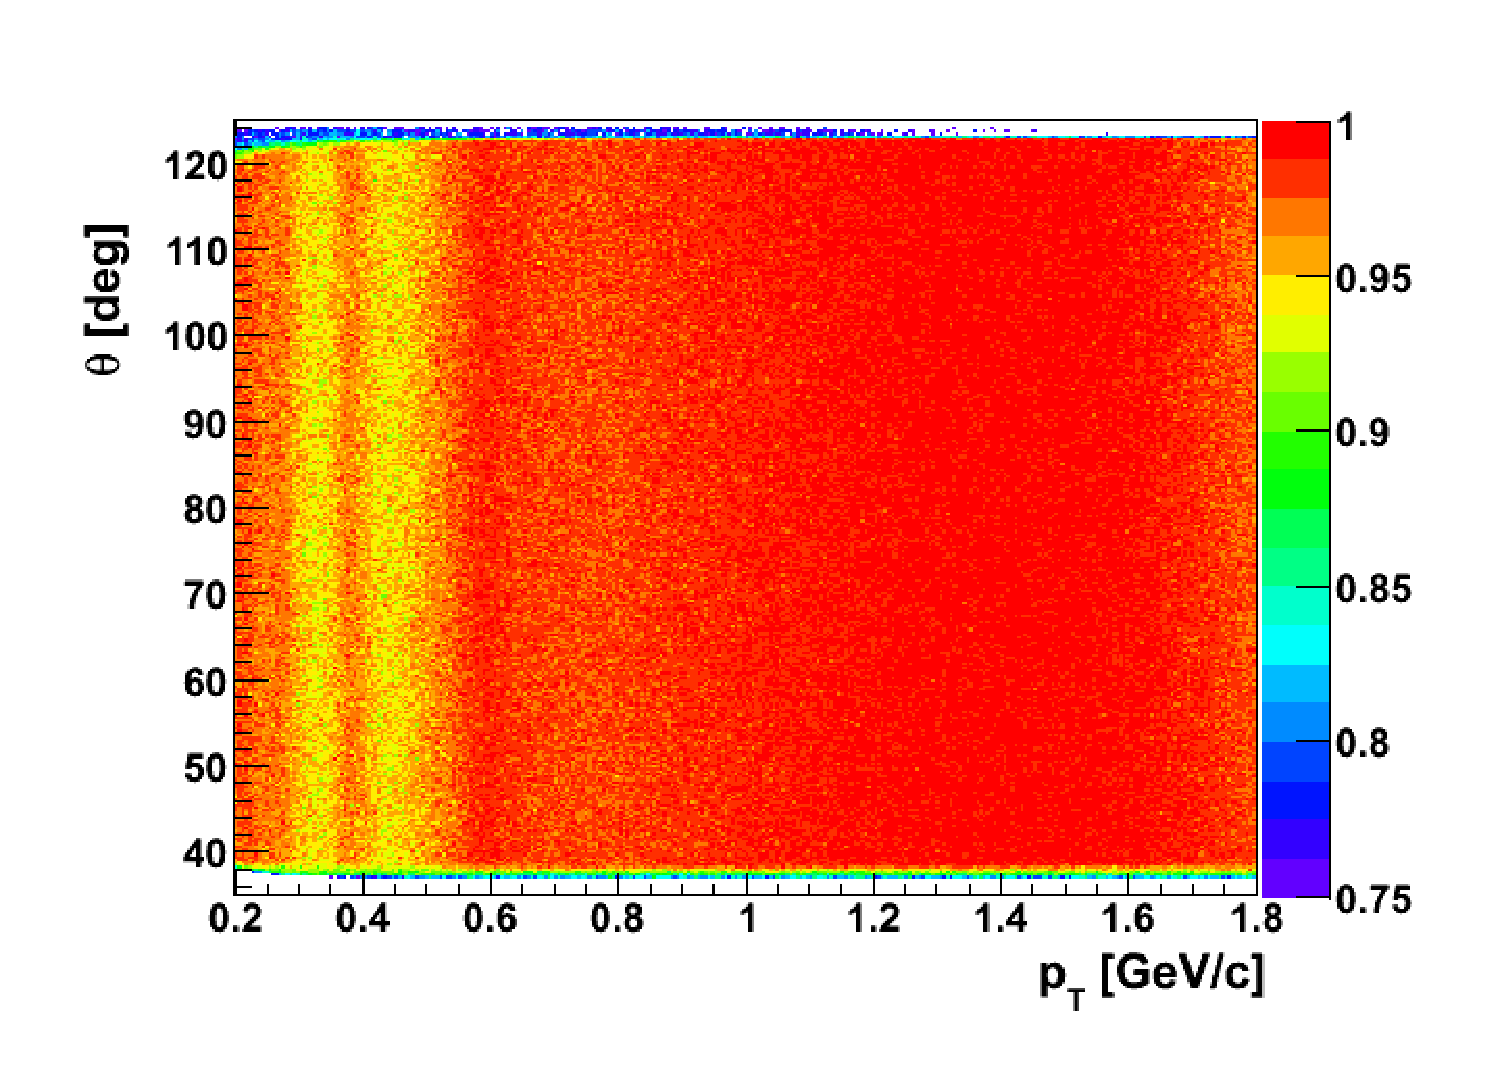
\includegraphics[width=0.49\textwidth]{SVT_2deff_thetapT.eps}
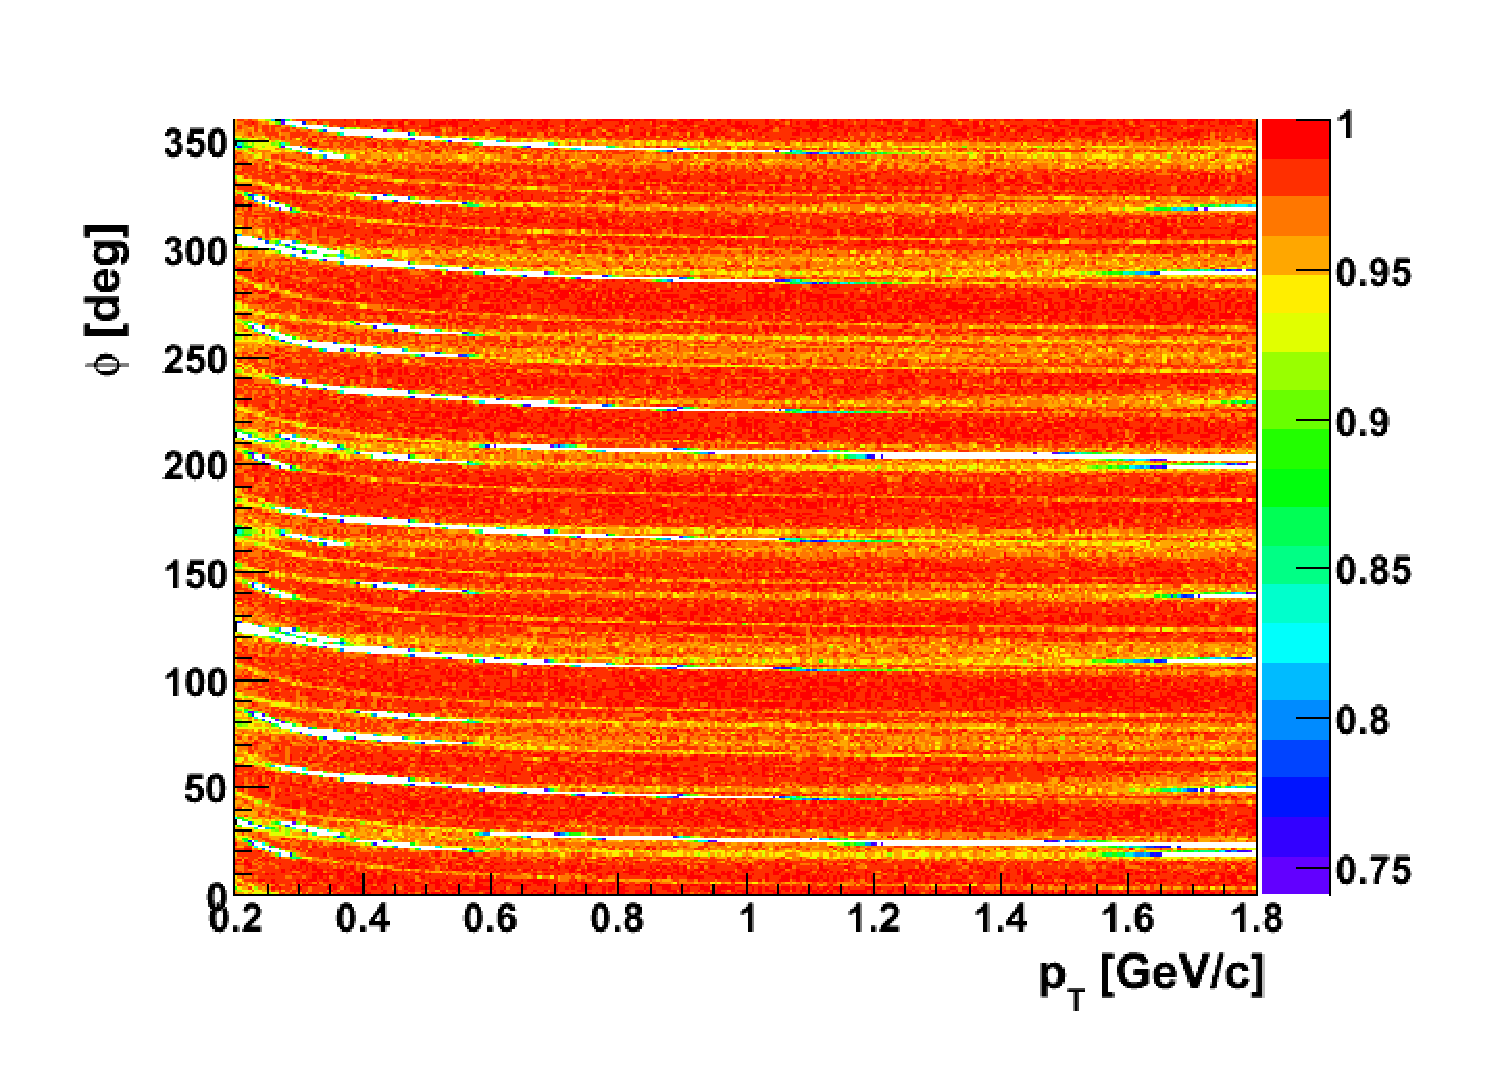
\includegraphics[width=0.49\textwidth]{SVT_2deff_phipT.eps}
\caption{\small{Track finding efficiency as a function of the transverse momentum 
$p_T$ and the polar angle $\theta$ (left) or the azimuthal angle $\phi$ (right).}}
\label{sec_central:pic_eff2d}
\end{figure}
%%%%%%%%%%%%%%%%%%%%%%%%%%%%%%%%%%%%%%%%%%%%%%%%%%%%%%%%%%%%%%%%%%%%%%%%%%%

For a 1-mm long target, the integrated efficiency is:

\begin{equation}
\langle \epsilon \rangle = 94\%.
\end{equation}

\noindent
For a 10-cm long target, this efficiency is around 90\%.  If we use only 3 double 
layers (no redundancy), the inefficiency reaches around 1/3.

\paragraph{Track Fitting:}

Once good track candidates have been identified, the corresponding list of hits is 
sent to the fitter algorithm.  This algorithm is based on the Kalman Filter that we 
described in Section~\ref{sec_KF}.  An important issue is the initialization of the 
state vector and its corresponding covariance matrix.  An analytic estimation of 
$\vec{x}$ is obtained assuming the track is a helix, the solenoid field being quite 
homogeneous across the entire BST.  The initial covariance matrix we choose is 
diagonal, with \emph{relatively} large values for the diagonal terms: around 2~mm for 
the $z$ uncertainty, 1$^\circ$ for $\phi$, 40~MeV for $p_x$ and $p_y$, and 100~MeV 
for $p_z$.  We also introduced a $p_T$ dependence on these terms to take into account 
the uncertainty due to the multiple scattering.  A further improvement would be to 
also introduce a $\theta$ dependence, as small biases were observed for angles close 
to 35$^\circ$ and 125$^\circ$.

Finally, the Kalman Filter is run, starting from the last available measurement, and 
going backwards.  It is stopped when it reaches the distance of closest approach to 
the beam axis, the corresponding point defining the \emph{vertex} of the current 
track.

\subsubsection{Tracking Performance}

The resolutions in $p_T$, $\theta$, $\phi$, and $z$ have been obtained using proton 
tracks at 90$^\circ$.  Because of the multiple scattering, these resolutions depend 
on the transverse momentum, and we used the following expressions to fit the different 
distributions:

\begin{equation}
\sigma_{p_T}/p_T = \sqrt{\left(\sigma_{1,p}\times p\right)^2
+\left(\frac{\sigma_{2,p}}{p\beta}\right)^2}
\end{equation}

\begin{equation}
\sigma_{\theta} = \sqrt{\left(\sigma_{1,\theta}\right)^2
+\left(\frac{\sigma_{2,\theta}}{p\beta}\right)^2}
\end{equation}

\begin{equation}
\sigma_{\phi} = \sqrt{\left(\sigma_{1,\phi}\times p\right)^2
+\left(\frac{\sigma_{2,\phi}}{p\beta}\right)^2}
\end{equation}

\begin{equation}
\sigma_{z} = \sqrt{\left(\sigma_{1,z}\times p\right)^2
+\left(\frac{\sigma_{2,z}}{p\beta}\right)^2}.
\end{equation}

\noindent
The 8 $\sigma_{i,X}$ extracted from the fits are summarized in 
Table~\ref{sec_central:table_resol}.  We see that the original requirements from 
Table~\ref{intro_requirements} are satisfied, even if we are at the upper limit for 
the $\theta$ resolution.

%%%%%%%%%%%%%%%%%%%%%%%%%%%%%%%%%%%%%%%%%%%%%%%%%%%%%%%%%%%%%%%%%%%%%%%%%%%
\begin{table}[ht!]
\centering
\begin{tabular}{|c|c|c|}\hline
                   &  $\sigma_1$ &  $\sigma_2$   \\ \hline
$p$                & 2.72\%      &  1.06\% GeV    \\
$\theta$           & 21.6 mrad   &  1.75 mrad GeV  \\
$\phi$             & 4.60 mrad   &  1.50 mrad GeV  \\
$z$                & 2.30 mm     &  0.13 mm GeV    \\ \hline
\end{tabular}
\caption{\small{Resolutions obtained in the central tracker for protons tracks at 
90$^\circ$.}}
\label{sec_central:table_resol}
\end{table}
%%%%%%%%%%%%%%%%%%%%%%%%%%%%%%%%%%%%%%%%%%%%%%%%%%%%%%%%%%%%%%%%%%%%%%%%%%%

The performance obtained with the Kalman Filter algorithm were also compared with 
estimates that can be analytically derived using the MOMRES program~\cite{momres}. 
To do this, we used only tracks with hits in all the double layers. 
Fig.~\ref{sec_central:pic_momrescomparison} shows that very good agreement is found 
between the two estimates, thus giving us confidence in our tracking code.  We can 
also note that the $p_T$ dependence of the obtained resolutions is very close to the 
expected ones (used for the fits).

%%%%%%%%%%%%%%%%%%%%%%%%%%%%%%%%%%%%%%%%%%%%%%%%%%%%%%%%%%%%%%%%%%%%%%%%%%%
\begin{figure}[ht!]
\centering
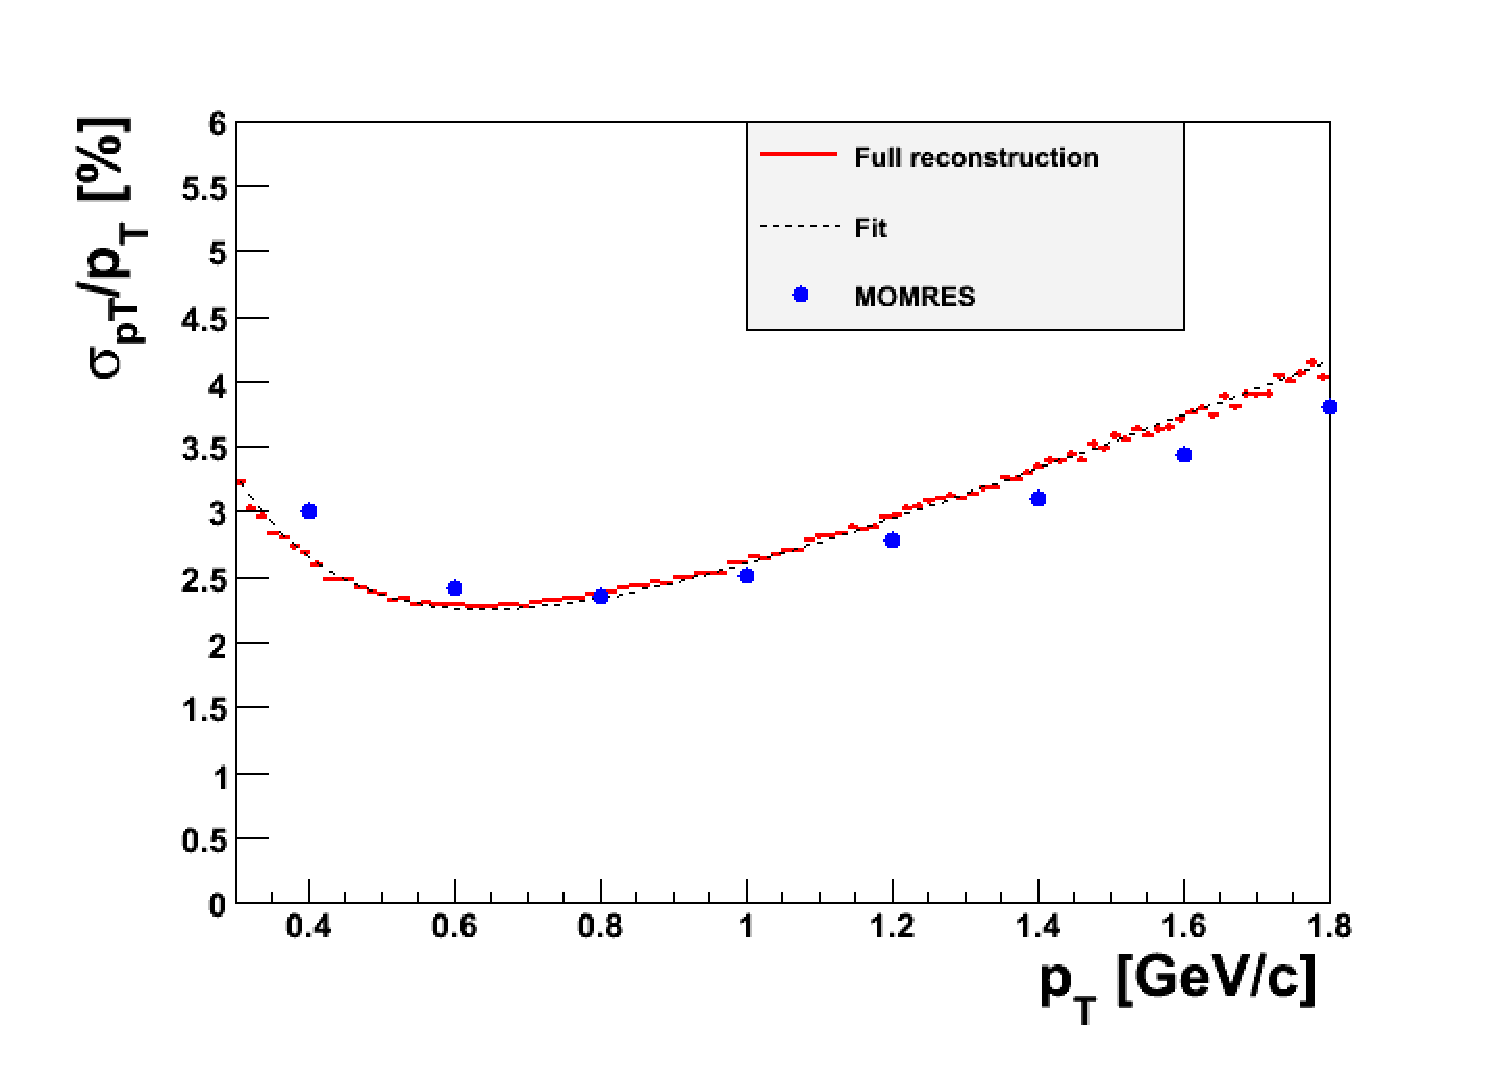
\includegraphics[width=0.49\textwidth]{sigmaptopt_VS_pT_SVTreal_theta60_4outof4_withfit.eps}
\includegraphics[width=0.49\textwidth]{sigmaphi_VS_pT_SVTreal_theta60_4outof4_withfit.eps}
\caption{\small{Comparison of the resolution in $p_T$ (left) and $\phi$ (right) 
obtained with the full reconstruction code and with the MOMRES program (proton tracks 
at $\theta$ = 60$^\circ$).}}
\label{sec_central:pic_momrescomparison}
\end{figure}
%%%%%%%%%%%%%%%%%%%%%%%%%%%%%%%%%%%%%%%%%%%%%%%%%%%%%%%%%%%%%%%%%%%%%%%%%%%

Finally, Table~\ref{sec_central:table_resolangle} shows the effect of the maximum 
strip angle on the resolutions, using the sample of tracks that has been used for 
the MOMRES comparison.  We see that the $\theta$ resolution can be improved 
significantly by using a larger angle, without significantly affecting the $p_T$ and 
$\phi$ resolutions.  However, a larger crossing angle will increase the 
reconstruction of fake tracks in the presence of background, which still needs to be 
quantified.

%%%%%%%%%%%%%%%%%%%%%%%%%%%%%%%%%%%%%%%%%%%%%%%%%%%%%%%%%%%%%%%%%%%%%%%%%%%
\begin{table}[ht!]
\centering
\begin{tabular}{|c|c|c|c|c|} \hline
$\alpha_{max}$ ($^{\circ}$) & $\sigma_{1,\theta}$ (mrad) & $\sigma_{1,p}$ (\%) & $\sigma_{1,\phi}$ (mrad) & $\sigma_{1,z}$ (mm)  \\ \hline
3    & 18.9   &  2.69  &    4.50   &  2.35  \\
6    & 12.0   &  3.04  &    5.09   &  1.43  \\
12   & 9.77   &  3.26  &    5.48   &  1.12  \\
15   & 8.74   &  4.05  &    6.66   &  0.93  \\ \hline
\end{tabular}
\caption{\small{Evolution of the resolutions with the maximum strip angle 
$\alpha_{max}$.}}
\label{sec_central:table_resolangle}
\end{table}
%%%%%%%%%%%%%%%%%%%%%%%%%%%%%%%%%%%%%%%%%%%%%%%%%%%%%%%%%%%%%%%%%%%%%%%%%%%

\subsubsection{Effect of the Background}

Background hits in the BST can degrade the tracking resolution, and produce fake 
tracks that will complicate the data analysis.  The first case happens when a fake 
hit is accidentally close to a good one, creating a \emph{sister} track that is 
similar to the original one.  But thanks to the good spatial resolution of the BST, 
only very close sister tracks can pass all the tracking filters (including a final 
$\chi^2$ cut), so that the effect on the resolution is very limited.  The creation 
of purely fake tracks, on the other hand, can be more problematic, and needs precise 
simulation on the background rate to be estimated.

The total number of tracks reconstructed in the BST for single particle events with 
uncorrelated background is presented in Fig.~\ref{sec_central:pic_background}.  We 
see that below 100~MHz per BST layer, the number of reconstructed tracks is rather 
limited, but tends to increase more rapidly above 100~MHz.  A detailed analysis shows 
that below this critical rate, additional tracks are mainly sister tracks, whereas 
they are essentially fakes above, when the density of hits is high enough.

%%%%%%%%%%%%%%%%%%%%%%%%%%%%%%%%%%%%%%%%%%%%%%%%%%%%%%%%%%%%%%%%%%%%%%%%%%%
\begin{figure}[ht!]
\centering
\includegraphics[width=0.7\textwidth]{SVT_trackcand_vs_rate.eps}
\caption{\small{Number of reconstructed tracks for single track events as a function 
of the (uncorrelated) background rate in the BST (see text for details).}}
\label{sec_central:pic_background}
\end{figure}
%%%%%%%%%%%%%%%%%%%%%%%%%%%%%%%%%%%%%%%%%%%%%%%%%%%%%%%%%%%%%%%%%%%%%%%%%%%

More detailed simulations were done using GEANT3 and GEANT4 they indicated that, 
with a luminosity of 10$^{35}$~cm$^{-2}$s$^{-1}$, the background rates do not 
exceed 60~MHz in the BST, i.e. well below the critical 100~MHz limit.  But they 
also showed that the background is slightly correlated, so a few fake tracks are 
indeed seen, as illustrated in Fig.~\ref{sec_central:pic_dvcs}.  However, the 
Central Time-Of-Flight (CTOF) allows for rejection of some of them (see 
Fig.~\ref{sec_central:pic_dvcs} left), thanks to its very good time resolution.  
The remaining tracks have almost the same momentum as the original one (\emph{sister} 
tracks, see Fig.~\ref{sec_central:pic_dvcs} right).  Using a merging algorithm for 
these tracks (to be written), the overall reconstructed events will be clean enough 
for most of the data analyses.

%%%%%%%%%%%%%%%%%%%%%%%%%%%%%%%%%%%%%%%%%%%%%%%%%%%%%%%%%%%%%%%%%%%%%%%%%%%
\begin{figure}[ht!]
\centering
\includegraphics[width=0.49\textwidth]{EvtDisplay_fullLumi_newDVCS_event52_20keVcut_ctof_1MeVcut.eps}
\includegraphics[width=0.49\textwidth]{ptrecons_Edepgt20keV.eps}
\caption{\small{(Left): DVCS event generated with GEANT4 at full luminosity.  The 
proton track (indicated by the pink line) has been correctly identified.  Two fake 
tracks are also visible, but can be rejected using the CTOF information. (Right): 
reconstructed momentum of tracks from DVCS events. On average, three tracks per event 
are reconstructed, most of them are very close to the original one.}}
\label{sec_central:pic_dvcs}
\end{figure}
%%%%%%%%%%%%%%%%%%%%%%%%%%%%%%%%%%%%%%%%%%%%%%%%%%%%%%%%%%%%%%%%%%%%%%%%%%%

\subsubsection{Misalignments}

All the resolutions and performances presented up to now assume a perfectly aligned 
BST.  In practice, many reasons -- from manufacturing to installation -- can 
introduce misalignments~\cite{2008-009}, thus degrading the resolution, not to 
mention introducing systematic shifts in momentum or angles.  To study these effects, 
we studied the use of different geometrical parameters in the track generation and 
the track reconstruction routines of Socrat.  For each BST double layer, the following 
parameters can be misaligned:

\begin{itemize}
\item its radius $R$ (expansion/contraction);
\item its global $\phi$ (rotation around the beam axis);
\item its $z$ position (translation along the beam axis).
\end{itemize}

In practice, one specifies the accuracy of the alignment for all these parameters 
(the accuracy can be different between two double layers), and the program generates 
misalignments on Gaussians with the corresponding widths.  The average effect on the 
resolution can then be estimated by running the program many of times to avoid bias 
from particular configurations.  Fig.~\ref{sec_central:pic_misalignR} illustrates the 
effect of misalignment in $R$.  On the left plot, no misalignments are introduced: 
the resolution found is independent of the sample of events, and no systematic shifts 
in momentum are observed.  On the right plot, one can see that a 200~$\mu$m accuracy 
on $R$ has a limited effect on the momentum resolution, but introduces a shift in 
momentum of the order of 0.8\%.

%%%%%%%%%%%%%%%%%%%%%%%%%%%%%%%%%%%%%%%%%%%%%%%%%%%%%%%%%%%%%%%%%%%%%%%%%%%
\begin{figure}[ht!]
\centering
\includegraphics[width=0.49\textwidth]{BST_misalignment_SigmaR0microns.eps}
\includegraphics[width=0.49\textwidth]{BST_misalignment_SigmaR200microns.eps}
\caption{\small{Momentum resolution and shift of 0.6~GeV protons at 60$^\circ$ 
without any misalignment (left) and with $R$ misalignment of 200~$\mu$m (right). 
Each entry of these histograms corresponds to a sample of 50k tracks, and a setup 
with misalignments randomly generated with a Gaussian of 0 and 200~$\mu$m widths,
respectively.}}
\label{sec_central:pic_misalignR}
\end{figure}
%%%%%%%%%%%%%%%%%%%%%%%%%%%%%%%%%%%%%%%%%%%%%%%%%%%%%%%%%%%%%%%%%%%%%%%%%%%

As this shift is the largest effect of misalignment, it has been studied as a 
function of misalignments in $R$ and $\phi$ (the misalignment in $z$ has almost no 
effect on momentum resolution, and limited effect on other track parameters).  These 
studies are summarized in Fig.~\ref{sec_central:pic_misalignRPhi}.  If we want to 
keep the momentum shift below 0.5\%, the plots tell us we need an accuracy:

\begin{itemize}
\item better than 100 microns in $R$;
\item better than 0.2 mrad in $\phi$.
\end{itemize}

%%%%%%%%%%%%%%%%%%%%%%%%%%%%%%%%%%%%%%%%%%%%%%%%%%%%%%%%%%%%%%%%%%%%%%%%%%%
\begin{figure}[ht!]
\centering
\includegraphics[width=0.49\textwidth]{MomShift_vs_Rmisalign.eps}
\includegraphics[width=0.49\textwidth]{MomShift_vs_Phimisalign.eps}
\caption{\small{Typical size of the momentum shift as a function of misalignments in 
$R$ (left) and $\phi$ (right) (0.6~GeV protons at 60$^\circ$).}}
\label{sec_central:pic_misalignRPhi}
\end{figure}
%%%%%%%%%%%%%%%%%%%%%%%%%%%%%%%%%%%%%%%%%%%%%%%%%%%%%%%%%%%%%%%%%%%%%%%%%%%

\noindent
These constraints seem to be compatible with what can be reasonably achieved.

Finally, we checked that misalignments in all the variables simultaneously have 
effects that are compatible with the ones obtained with separate misalignments, as 
illustrated in Fig.~\ref{sec_central:pic_misalignRZPhi}.

%%%%%%%%%%%%%%%%%%%%%%%%%%%%%%%%%%%%%%%%%%%%%%%%%%%%%%%%%%%%%%%%%%%%%%%%%%%
\begin{figure}[ht!]
\centering
\includegraphics[width=0.49\textwidth]{BST_misalignment_SigmaR50microns_SigmaZ20microns_SigmaPhi01mrad.eps}
\includegraphics[width=0.49\textwidth]{BST_misalignment_SigmaR200microns_SigmaZ100microns_SigmaPhi1mrad.eps}
\caption{\small{Momentum resolution and shift of 0.6~GeV protons at 60$^\circ$ with 
two different sets of misalignments: $\delta$$R$ = 50~$\mu$m; $\delta$$z$ = 20~$\mu$m; 
$\delta$$\phi$ = 0.1 mrad (left); $\delta$$R$ = 200~$\mu$m; $\delta$$z$ = 100~$\mu$m; 
$\delta$$\phi$ = 1 mrad (right).}}
\label{sec_central:pic_misalignRZPhi}
\end{figure}
%%%%%%%%%%%%%%%%%%%%%%%%%%%%%%%%%%%%%%%%%%%%%%%%%%%%%%%%%%%%%%%%%%%%%%%%%%%

\subsection{Forward Tracking}
\label{sec_forward}

\subsubsection{DC and FST Design}

The FST allows the detection of particles between 5$^\circ$ and 35$^\circ$.  Its 
major component is a set of 36 planes of Drift Chambers, divided in three regions of 
two superlayers each, ensuring highly efficient detection with large redundancy. 
Each region is divided in six sectors of 60$^\circ$, each of them containing six 
planes of 112 wires.  From studies of the current {\tt CLAS} DC, the space resolution 
is expected to be around 250--300~$\mu$m.  The momentum determination will be provided 
by the use of a toroidal magnetic field surrounding Region~2.

The other element of this tracker is the FST, which consists of three double layers of 
silicon strips located between the target and the DC.  Each layer is made with 15 
trapezoids, with stereo strip angles of $\pm$12$^\circ$.  

\subsubsection{Tracking in the DC}

The tracking in the Drift Chambers is performed in three successive steps that will be 
described below:

\begin{itemize}
\item first, we look for combinations of \emph{clusters} that can define a track 
candidate;
\item then we identify a \emph{road} in each of the selected clusters (and solve the 
left-right ambiguity of the corresponding hits);
\item finally we run the Kalman Filter algorithm on the track candidates for which 
roads were successfully identified.
\end{itemize}

\paragraph{Cluster and Track Finding:}

If a particle goes through a DC superlayer, it will leave a collection of hits 
forming a continuous series of wire numbers (e.g. wire number 37 in first plane, 38 
in second, 37 in third, etc.).  The very first step of the tracking is therefore to 
loop over all the hits of an event to find these series (called \emph{clusters}), 
with hits in all the planes of the current superlayer.  To have overall fast and 
efficient tracking, the number of found clusters should be limited, so the occupancy 
in the DC should not exceed a few percent, as illustrated in 
Fig.~\ref{sec_forward:pic_Nclusters}.

%%%%%%%%%%%%%%%%%%%%%%%%%%%%%%%%%%%%%%%%%%%%%%%%%%%%%%%%%%%%%%%%%%%%%%%%%%%
\begin{figure}[ht!]
\centering
\includegraphics[width=0.7\textwidth]{Ncluster_vs_occupancy.eps}
\caption{\small{Evolution of the number of clusters per DC superlayer for single 
track events with (uncorrelated) background.}}
\label{sec_forward:pic_Nclusters}
\end{figure}
%%%%%%%%%%%%%%%%%%%%%%%%%%%%%%%%%%%%%%%%%%%%%%%%%%%%%%%%%%%%%%%%%%%%%%%%%%%

The next step is to form a \emph{track segment} candidate, that is a combination of 
two close clusters in a given region. for real tracks, the average wire numbers 
$W_1$ and $W_2$ of two consecutive clusters satisfy the inequality 
$|W_1$ - $W_2|$ $<$ $K\times$$W_1$, with $K$ around 0.15.  In practice, we obtained 
a cluster matching efficiency close to 100\% by using:

\begin{equation}
|W_1-W_2| < 0.18 \times W_1 + 5.
\end{equation}

Finally, we look for a combination of track segments in all the DC regions that could 
define a track candidate.  As the number of track segments is limited with the 
expected occupancy, we simply require at this stage that they all are in a single 
sector.  The very few remaining bad candidates will be rejected during the fitting 
procedure.

The result of the track finding is illustrated in 
Fig.~\ref{sec_forward:pic_trackfinding}, which shows the initial distribution of hits 
in the DC, and the final remaining candidates.

%%%%%%%%%%%%%%%%%%%%%%%%%%%%%%%%%%%%%%%%%%%%%%%%%%%%%%%%%%%%%%%%%%%%%%%%%%%
\begin{figure}[ht!]
\centering
\includegraphics[width=0.6\textwidth]{DC_clusterfinding_step0.eps}
\includegraphics[width=0.6\textwidth]{DC_clusterfinding_step3.eps}
\caption{\small{(Top): distribution of initial hits in all the DC planes (single track 
event with 10\% uncorrelated occupancy); (bottom): remaining track candidates.}}
\label{sec_forward:pic_trackfinding}
\end{figure}
%%%%%%%%%%%%%%%%%%%%%%%%%%%%%%%%%%%%%%%%%%%%%%%%%%%%%%%%%%%%%%%%%%%%%%%%%%%

\paragraph{Road Finding:}

Even without any background, a real cluster cannot be used directly for the fit, as 
left-right ambiguities should be solved.  In the presence of background, a real 
cluster may also contain fake hits that are accidentally close to the real ones.  To 
solve these two problems, we developed the following iterative procedure:

\begin{itemize}
\item we first try to fit each hit combination of a cluster with a straight line, in 
a plane perpendicular to the wire direction.  At this stage, we only use the wire 
position, with an uncertainty corresponding to the drift distance;
\item this preliminary fit allows us to discard some hits (on the edges of the 
cluster), and to solve, for a particular combination, some left-right ambiguities. 
The next iteration uses only the remaining hits, with the real hit position if the
left-right ambiguity has been solved.  The fits are then more and more precise, so 
that more and more ambiguities are solved;
\item after four iterations, all of the remaining ambiguities are solved using the 
latest fit.
\end{itemize}

Note that for the moment, the final road cannot contain more than one hit per plane, 
even if particles with large incidence angle can indeed leave two good hits within 
a single layer.

If the initial track is relatively close to a wire, it is sometimes not possible to 
decide whether it was on the left or on the right: in total, our procedure makes 
the correct decision for 90\% of the hits.  In the presence of background, this 
probability decreases, as a fake hit can ``kill'' a good one, or be close enough to 
be identified as good, and then spoil the fit.  However, this effect is limited, as 
shown in Fig.~\ref{sec_forward:pic_roadsincluster}, proving that our procedure is 
relatively robust.

%%%%%%%%%%%%%%%%%%%%%%%%%%%%%%%%%%%%%%%%%%%%%%%%%%%%%%%%%%%%%%%%%%%%%%%%%%%
\begin{figure}[ht!]
\centering
\includegraphics[width=0.7\textwidth]{wrongLR_vs_occupancy.eps}
\caption{\small{Probability to wrongly solve the left-right ambiguity as a function 
of the DC occupancy.}}
\label{sec_forward:pic_roadsincluster}
\end{figure}
%%%%%%%%%%%%%%%%%%%%%%%%%%%%%%%%%%%%%%%%%%%%%%%%%%%%%%%%%%%%%%%%%%%%%%%%%%%

\paragraph{Track Fitting:}

The final sets of hits are then sent to the Kalman Filter algorithm, as for the 
central part.  Because of the geometry of the Forward Tracker (measurements at 
approximately constant $z$), the state vector chosen is now:

\begin{equation}
\vec{x} = (x, y, u_x, u_y, Q/p)^T,
\end{equation}

\noindent
where $x$ and $y$ are the coordinates in a plane perpendicular to the beam axis, 
$u_x$ and $u_y$ are the slopes of the projected track in the $xz$ and $yz$ planes, 
respectively, and $Q/p$ is the charge divided by the momentum.

The first four components of this state vector are easily initialized at the last 
plane of Region~3.  The last component is estimated using the angles before (using a 
linear fit in Region~1) and after (using Region~3) the toroidal field, $\theta_1$ 
and $\theta_3$.  We then use the well known formula:

\begin{equation}
Q/p = \frac{\theta_3-\theta_1}{0.3\times \int{Bdl}},
\end{equation}

\noindent
with a parameterization of the field integral $\int{Bdl}$ as a function of the 
position in Region~1 (this parameterization is different for positively and negatively
charged particles).

The initial uncertainties on these components (used in the covariance matrix) were 
chosen to be 3~cm for the position terms, 80~mrad for the slopes, and 50\% for $Q/p$.

As for the central part, the fit is then stopped at the closest distance to the beam 
axis.  However, for some specific reactions, we may want to determine the vertex 
position more accurately, and the DC are then used in combination with the FST.  The 
key issue is then the accuracy of the extrapolation of the track parameters between 
the first DC plane and the last FST layer (located more than 2~m upstream).

\subsubsection{Matching with the FST}

The track finding procedure in the FST is quite simple, as the double layers are very 
close to each other, so track candidates are almost straight lines.  We therefore 
select combinations of strips producing three almost aligned points in space, 
pointing not too far from the beam axis.  The corresponding cuts have been optimized 
to identify at least 99\% of the \emph{reconstructable} tracks.

As the FST is always used with the DC, and not as a standalone tracker, we do not 
need \emph{a priori} to require a hit in each layer.  However, all the dead zones are 
aligned in the current design, so that a particle missing one layer will miss at least 
another one with a probability of around 99.5\%.  Besides, requiring only two out of 
three double layers increases the reconstruction of fake tracks by a large factor. 
We thus require three out of three double layers to define a track candidate in the 
FST.  The resulting acceptance efficiency is shown in Fig.~\ref{sec_forward:pic_FSTeff} 
as a function of the polar and azimuthal angles of the particles.

%%%%%%%%%%%%%%%%%%%%%%%%%%%%%%%%%%%%%%%%%%%%%%%%%%%%%%%%%%%%%%%%%%%%%%%%%%%
\begin{figure}[ht!]
\centering
\includegraphics[width=0.7\textwidth]{FVT_2deff_phitheta_thintarget.eps}
\caption{\small{Acceptance efficiency of the FST as a function of the polar and 
azimuthal angles of the tracks, requiring three out of three double layers.}}
\label{sec_forward:pic_FSTeff}
\end{figure}
%%%%%%%%%%%%%%%%%%%%%%%%%%%%%%%%%%%%%%%%%%%%%%%%%%%%%%%%%%%%%%%%%%%%%%%%%%%

For a 1-mm long target, the integrated efficiency of the FST is:

\begin{equation}
\langle \epsilon \rangle = 92\%.
\end{equation}

\noindent
The next step is to be able to match track candidates from the FST and from the DC. 
To do this, we run the Kalman Filter algorithm on DC candidates, extrapolate down 
to the FST, and look for a \emph{close} FST candidate.  The accuracy of this 
extrapolation should be good enough not to match with another track (fake or not). 
Fig.~\ref{sec_forward:pic_matching} shows that, for a large fraction of tracks, the 
extrapolated position is within a few mm circle around the original position of the 
particle.  A 1-cm cut is therefore applied on the distance between the extrapolation 
and the FST track to match the two candidates.  This allows a 98\% matching efficiency 
without background; the effect of the DC occupancy (that deteriorates the accuracy of 
the fit) is shown in Fig.~\ref{sec_forward:pic_matcheff}.

%%%%%%%%%%%%%%%%%%%%%%%%%%%%%%%%%%%%%%%%%%%%%%%%%%%%%%%%%%%%%%%%%%%%%%%%%%%
\begin{figure}[ht!]
\centering
\includegraphics[width=0.49\textwidth]{CircleConfusion_theta15_proton_DCocc0_FVT0MHz.eps}
\includegraphics[width=0.49\textwidth]{CircleConfusion_theta15_proton_DCocc4_FVT40MHz.eps}
\caption{\small{$xy$ distribution of the DC track extrapolated down to the last FST 
layer with respect to the original position of the track. (Left): without any 
background; (right): with a 4\% occupancy in the DC.}}
\label{sec_forward:pic_matching}
\end{figure}
%%%%%%%%%%%%%%%%%%%%%%%%%%%%%%%%%%%%%%%%%%%%%%%%%%%%%%%%%%%%%%%%%%%%%%%%%%%

%%%%%%%%%%%%%%%%%%%%%%%%%%%%%%%%%%%%%%%%%%%%%%%%%%%%%%%%%%%%%%%%%%%%%%%%%%%
\begin{figure}[ht!]
\centering
\includegraphics[width=0.6\textwidth]{matchingEff_vs_occupancy.eps}
\caption{\small{FST-DC matching efficiency as a function of the DC occupancy.  A
4\% occupancy degrades the efficiency by around 10\%.}}
\label{sec_forward:pic_matcheff}
\end{figure}
%%%%%%%%%%%%%%%%%%%%%%%%%%%%%%%%%%%%%%%%%%%%%%%%%%%%%%%%%%%%%%%%%%%%%%%%%%%

When the matching is successful, it appears that the fit is too unstable to be 
performed in a single step.  We thus introduced some iterations as follows: in a 
first step, the Kalman Filter fits the track backwards, assuming a larger space 
resolution for the FST (7 times larger); the track is then extrapolated forwards, 
and refit using only the DC.  The final fit is performed backwards again, using the 
real resolution for the FST.  We are now able to derive the resolutions obtained in 
the Forward Tracker, and to study the effect of the FST.

\subsubsection{Tracking Performance}

The resolutions of momentum, polar angle $\theta$, azimuthal angle $\phi$, vertex 
position $z$, and distance of closest approach to the beam axis $b$ are presented in 
Fig.~\ref{sec_forward:pic_resolproton} for proton tracks at 15$^\circ$, using the DC 
alone, or in combination with the FST.  Fig.~\ref{sec_forward:pic_resolelectron} shows 
the same resolutions for electron tracks.  The effect of the DC occupancy on the 
resolution is very limited, as illustrated in Fig.~\ref{sec_forward:pic_phiresol} for 
the $\phi$ resolution.

%%%%%%%%%%%%%%%%%%%%%%%%%%%%%%%%%%%%%%%%%%%%%%%%%%%%%%%%%%%%%%%%%%%%%%%%%%%
\begin{figure}[ht!]
\centering
\includegraphics[width=0.29\textwidth]{DC_vs_DCFVT_theta15_sigmapop_DCocc4_FVT40MHz.eps}
\includegraphics[width=0.29\textwidth]{DC_vs_DCFVT_theta15_sigmatheta_DCocc4_FVT40MHz.eps}
\includegraphics[width=0.29\textwidth]{DC_vs_DCFVT_theta15_sigmaphi_DCocc4_FVT40MHz.eps}
\includegraphics[width=0.29\textwidth]{DC_vs_DCFVT_theta15_sigmaz_DCocc4_FVT40MHz.eps}
\includegraphics[width=0.29\textwidth]{DC_vs_DCFVT_theta15_sigmab_DCocc4_FVT40MHz.eps}
\caption{\small{Resolutions in $p$, $\theta$, $\phi$, $z$, and $b$ (distance of 
closest approach to the beam axis) for 15$^\circ$ protons with and without the FST. 
A 4\% occupancy in the DC and 40~MHz in the FST have been assumed.}}
\label{sec_forward:pic_resolproton}
\end{figure}
%%%%%%%%%%%%%%%%%%%%%%%%%%%%%%%%%%%%%%%%%%%%%%%%%%%%%%%%%%%%%%%%%%%%%%%%%%%

%%%%%%%%%%%%%%%%%%%%%%%%%%%%%%%%%%%%%%%%%%%%%%%%%%%%%%%%%%%%%%%%%%%%%%%%%%%
\begin{figure}[ht!]
\centering
\includegraphics[width=0.29\textwidth]{DC_vs_DCFVT_electrons_theta15_sigmapop_DCocc4_FVT40MHz.eps}
\includegraphics[width=0.29\textwidth]{DC_vs_DCFVT_electrons_theta15_sigmatheta_DCocc4_FVT40MHz.eps}
\includegraphics[width=0.29\textwidth]{DC_vs_DCFVT_electrons_theta15_sigmaphi_DCocc4_FVT40MHz.eps}
\includegraphics[width=0.29\textwidth]{DC_vs_DCFVT_electrons_theta15_sigmaz_DCocc4_FVT40MHz.eps}
\includegraphics[width=0.29\textwidth]{DC_vs_DCFVT_electrons_theta15_sigmab_DCocc4_FVT40MHz.eps}
\caption{\small{Resolutions in $p$, $\theta$, $\phi$, $z$, and $b$ (distance of 
closest approach to the beam axis) for 15$^\circ$ electrons with and without the 
FST.  A 4\% occupancy in the DC and 40~MHz in the FST have been assumed.}}
\label{sec_forward:pic_resolelectron}
\end{figure}
%%%%%%%%%%%%%%%%%%%%%%%%%%%%%%%%%%%%%%%%%%%%%%%%%%%%%%%%%%%%%%%%%%%%%%%%%%%

%%%%%%%%%%%%%%%%%%%%%%%%%%%%%%%%%%%%%%%%%%%%%%%%%%%%%%%%%%%%%%%%%%%%%%%%%%%
\begin{figure}[ht!]
\centering
\includegraphics[width=0.7\textwidth]{phiResol_vs_occupancy.eps}
\caption{\small{Evolution with the DC occupancy of the $\phi$ resolution (the 
$p$ independent term) in the forward tracker.}}
\label{sec_forward:pic_phiresol}
\end{figure}
%%%%%%%%%%%%%%%%%%%%%%%%%%%%%%%%%%%%%%%%%%%%%%%%%%%%%%%%%%%%%%%%%%%%%%%%%%%

If we compare with the original requirements from Table~\ref{intro_requirements}, 
we see that the DC design satisfies all of the proposed performances.  Concerning 
the FST, it largely improves the vertex determination (up to a factor 10 on $b$), 
and also allows a better determination of $p$ and $\phi$ at large momenta.

\subsubsection{Misalignments}

As for the BST, we implemented in Socrat the possibility to misalign the detectors 
or the magnetic fields.  For a given region of the DC, the following parameters can 
be misaligned:

\begin{itemize}
\item the distance $R$ to the target;
\item the tilt around its local $x'$ axis (25$^\circ$ being the nominal value);
\item the distance of the first wire to the beam axis.
\end{itemize}

\noindent
Two parameters of an FST double layer can also be misaligned.  These are:

\begin{itemize}
\item its azimuthal position $\phi$;
\item its position along the beam axis $z$.
\end{itemize}

\noindent
Finally, Socrat can misalign the toroidal field in $x$, $y$, and $z$, with respect 
to the rest of the spectrometer.

Due to the large number of parameters, we illustrate only the effect of misalignment 
in $R$ for Region~3 of the DC, and in $z$ for the torus, as shown in 
Fig.~\ref{sec_forward:pic_FTmisalign}.  We see that both the DC and the torus should 
be aligned within a fraction of a millimeter.  In general, our studies are consistent 
with the rule saying that a detector needs to be aligned within a fraction of its 
space resolution for a given parameter: e.g. less than 50~$\mu$m for the transverse 
position of the FST, and a few hundred microns for the longitudinal one (because of 
the angle of the tracks).

%%%%%%%%%%%%%%%%%%%%%%%%%%%%%%%%%%%%%%%%%%%%%%%%%%%%%%%%%%%%%%%%%%%%%%%%%%%
\begin{figure}[ht!]
\centering
\includegraphics[width=0.49\textwidth]{DCFVT_aligned_VS_DC3DR1mm_Deltapop.eps}
\includegraphics[width=0.49\textwidth]{DCFVT_aligned_VStorusDz10mm_Deltapop.eps}
\caption{\small{Effect of misalignments on the reconstructed momentum as a function 
of $p$: (left): $R$ translation of DC Region~3 by 1~mm; (right): $z$ translation of 
the toroidal field by 10~mm.}}
\label{sec_forward:pic_FTmisalign}
\end{figure}
%%%%%%%%%%%%%%%%%%%%%%%%%%%%%%%%%%%%%%%%%%%%%%%%%%%%%%%%%%%%%%%%%%%%%%%%%%%

\subsection{Conclusion}

We described in this section the program we developed for charged particle 
reconstruction with the {\tt CLAS12} spectrometer.  In the central and forward 
parts, track finding procedures, as well as a Kalman Filter algorithm, were 
successfully applied.  They provide for efficient reconstruction with resolutions 
that are in agreement with initial estimations and fulfill the physics requirements. 
The effect of the background has been quantified, and seems to be limited . 
Misalignments of all the detectors have also been studied, providing constraints on 
the position accuracy that will be needed, in particular for the BST.  For the 
Forward Tracker, we showed that a highly efficient matching can be obtained between 
the FST and DC tracks, and we quantify the large improvement of the FST on the 
vertex determination.

The global track reconstruction is however not yet finished.  More studies will be 
needed using GEANT4 simulations, particularly to study the effect of the correlated 
background on the tracking efficiency in the DC.  A vertex fit, gathering 
information from the central and forward regions, has to be developed.  Some smaller 
improvements can also be implemented, for example to take into account double hits 
from a single track in the DC.

\section{Expected Physics Performance}

We have used a series of programs to calculate the acceptance and 
reconstructed physics parameters for event types of interest.  The program 
CLASEV~\cite{clasev} served as an event generator and analysis program. 
Depending on the value of input flags, it generates certain types of events, 
that is, it produces a set of 4-momenta for the primary hadrons in the 
hadronic center-of-mass and allows some of them to decay into the final-state 
hadrons and transforms their momenta to the lab system.  For each final-state 
track, it calls FASTMC (our fast, parametric Monte Carlo program for
{\tt CLAS12}) to determine if the track falls within a fiducial acceptance 
window and to determine its final, smeared lab momentum.  It then produces 
selected physics analysis variables (e.g. missing mass) from calculations 
involving the smeared momenta of the tracks that were accepted. 
Fig.~\ref{massplot} shows the expected missing mass resolution expected for 
{\tt CLAS12} from FASTMC simulation studies based on the current design 
specifications for a number of different reactions.  For all cases studied, 
the results are quite encouraging in terms of identifying the missing 
particle cleanly for each reaction.  Our GEANT3 results are in accord
with the FASTMC results.

We also show some results from our FASTMC simulation of $e \pi^+$ events
in which the recoil baryon is detected by missing mass.  
Fig.~\ref{centralmassplot} shows the missing mass spectrum expected when
the $\pi^+$ is detected in the forward tracker (left) or central tracker
(right).  We have sufficient resolution to study resonant production and
to compare, for example, u-channel, s-channel and t-channel processes.

%%%%%%%%%%%%%%%%%%%%%%%%%%%%%%%%%%%%%%%%%%%%%%%%%%%%%%%%%%%%%%%%%%%%%%%%%%%
\begin{figure}[htbp]
\vspace{14.0cm}
\special{psfile=mm1.ps hscale=39 vscale=36 hoffset=0 voffset=160}
\special{psfile=mm2.ps hscale=39 vscale=36 hoffset=235 voffset=160}
\special{psfile=mm3.ps hscale=40 vscale=37 hoffset=0 voffset=-55}
\special{psfile=mm4.ps hscale=40 vscale=37 hoffset=240 voffset=-55}
\caption{\small{Simulation results from FASTMC highlighting the expected 
missing mass resolution of {\tt CLAS12} with the nominal design 
specifications for the tracking detectors (drift chambers and SVT).  Shown 
are the spectra for the reactions $ep \to e'\pi+X$ (UL), $ep \to e'K^+X$ (UR),
$ep \to e'p\pi^+X$ (LL), and $ep \to e\rho^+X$ (LR).}}
\label{massplot}
\end{figure}
%%%%%%%%%%%%%%%%%%%%%%%%%%%%%%%%%%%%%%%%%%%%%%%%%%%%%%%%%%%%%%%%%%%%%%%%%%%

%%%%%%%%%%%%%%%%%%%%%%%%%%%%%%%%%%%%%%%%%%%%%%%%%%%%%%%%%%%%%%%%%%%%%%%%%%%
\begin{figure}[htbp]
\vspace{6.0cm}
\special{psfile=clas12pipforward.eps hscale=39 vscale=36 hoffset=0 voffset=0}
\special{psfile=clas12pipcentral.eps hscale=39 vscale=36 hoffset=235 voffset=0}
\caption{\small{Simulation results from FASTMC highlighting the expected 
missing mass resolution of {\tt CLAS12} for events in which we detect only
a $\pi^+$ and the electron for two cases: on the left when the $\pi^+$
is detected in the forward tracker, and on the right when detected in
the central tracker.}}
\label{centralmassplot}
\end{figure}
%%%%%%%%%%%%%%%%%%%%%%%%%%%%%%%%%%%%%%%%%%%%%%%%%%%%%%%%%%%%%%%%%%%%%%%%%%%

\section{Safety and Quality Assurance Issues}

\subsection{Safety}

There are safety issues in the construction, installation, and operation
phases of the {\tt CLAS12} drift chamber and SVT projects that we address 
in this section.  Safety will be addressed from the start as an integral 
part of all activities and plans.  All of our workers will receive 
appropriate training prior to being permitted to perform any activities 
on the detectors.

\subsubsection{Drift Chamber}

Table~\ref{dc-safety} briefly summarizes the issues and the mitigation 
strategies employed for the drift chamber system.

%%%%%%%%%%%%%%%%%%%%%%%%%%%%%%%%%%%%%%%%%%%%%%%%%%%%%%%%%%%%%%%%%%%%%%%%%
\begin{table}[htbp]
\begin{center}
\begin{small}
\begin{tabular} {||c|c|c||} \hline \hline
{\bf Operation} & {\bf Issue}     &  {\bf Mitigation} \\ \hline
Cleaning parts  & Solvents & Use of non-volatiles; masks \\ \hline
Box assembly & Material handling, welding & Standard procedures \\ \hline
Stringing & Material handling  & Design overview, reviewed procedures \\ \hline
Installation & Material handling & Design overview, reviewed procedures \\ \hline
Gas delivery      & Flammability; ODH & Non-flammable mixture, small lines \\ \hline
Gas delivery      & Over/under pressure & Active controls, passive bubblers \\ \hline
LV power          & Over-heating & Each line individually fused \\ \hline
HV power          & Shock & Current-limited supplies, reviewed procedures \\ \hline
Routine operation & Sparking & Fast-trip supplies \\ \hline
Repair & Material handling & Design overview, reviewed procedures \\ \hline \hline
\end{tabular}
\end{small}
\caption{\small{Safety issues in the {\tt CLAS12} drift chamber project.}}
\label{dc-safety}
\end{center}
\end{table}
%%%%%%%%%%%%%%%%%%%%%%%%%%%%%%%%%%%%%%%%%%%%%%%%%%%%%%%%%%%%%%%%%%%%%%%%%

The only significant safety issues are in the construction, installation, 
and operation of the chambers.  During the construction phase, we receive 
a number of machined parts from industry that must be cleaned thoroughly 
before assembly into a chamber.  Our anticipated cleaning strategy is to 
use safe, non-volatile cleaning agents that are friendly to the environment 
and to human health.  All of our activities are coordinated by written 
procedures that are reviewed by our safety staff at the lab.

During construction of the chamber boxes, we handle heavy metallic items and 
bolt or weld certain items.  All of these activities are handled by personnel 
with adequate safety training, wearing suitable protective gear.  The designs 
of all mechanical assemblies are reviewed by trained mechanical engineers and 
experienced technicians.

During stringing of the chamber, the technicians and stringers work on 
elevated platforms.  The platform designs are reviewed in a similar fashion 
to the chamber mechanical designs, and all work is closely supervised by 
experienced technicians.

Operation of the chambers involves the use of a gas-handling system.  We use 
non-flammable gas mixtures delivered to the chambers at low pressure.  There 
are intermediate storage tanks filled with gas at moderate (a few atmospheres)
of pressure.  The gas-mixing and delivery system will be the same as the 
present {\tt CLAS} system with minor modifications, so we will continue to 
follow our present safety procedures that include some engineering controls 
in the gas-mixing shed to mitigate possible ODH conditions and extensive 
active and passive controls to mitigate over- and under-pressure conditions 
that could harm the drift chambers.

The normal operation also involves delivery of low-voltage power to the 
on-chamber amplifiers.  Although the low voltage (less than 8~V) means that 
there is no electrocution hazard, there is a potential for over-heating and 
fire ignition because of the relatively high currents involved.  Each supply 
is capable of supplying up to 50~mA of current.  Our mitigation strategy is 
to not allow more than 3~A of current on any output line, enforced by the 
placement of individual fuses on every wire that leaves the supply. 

The Hall B Drift Chamber Low Voltage (DCLV) supply and distribution system 
consists of 18 HP 6651A power supplies. Each power supply has a maximum 
current output of 8~VDC and 50~A of current. The power supplies are connected 
to the Hall B 120~VAC clean power located in the individual racks of the 
space frame that are protected by an electrical breaker panel. The supplies 
have a 10~A current limiting fuse for its own A.C. line protection.  The 
DCLV system supplies DC power to the drift chamber Signal Translator Boards 
(STBs). The output voltage can be set at the supply, as well as a current 
limit. In Hall B the current limits are individually set for each 
region/sector. The power is then supplied to the STBs via a distribution 
chassis.  Each chassis is safety interlocked and contains 3 bus bars 
(positive, negative, and earth ground), of which the positive and negative 
are connected to the individual STBs through current limiting fuses.  The 
individual fuses provide the nominal current draw plus 20\% for transient 
spikes. The distribution system for Region~3 was upgraded in 2003 to provide 
segmentation of the axial and stereo boards, thus reducing the damage of a 
permanent short by half. The upgrade consisted of adding new power wires 
from the distribution to the STBs and adding an additional breakout chassis. 
The breakout chassis provided individual fuses for each side of the STB in 
front of the distribution fuse.  Each breakout fuse is rated for the nominal 
current draw of its respective channel on the STB plus 40\% for transient 
spikes.  In the event of a short on the chamber there is a written procedure 
for changing out fuses located in the Hall B counting house and the drift 
chamber expert manual.  Monitoring of the supplies is done using a PC-based 
LabView program from the Hall B counting house.

Operation also involves the delivery of high-voltage to the drift chamber 
wires.  The operating voltages are between 1000 and 2000~V, depending on 
the section in question.  In all cases, the high voltage supplies are 
current-limited.  No channel can deliver more than 40~$\mu$A of current.  
Administrative procedures are in place to prevent accidental shocks from 
taking place.

The Hall B Drift Chamber High Voltage (DCHV) system consists of 3 CAEN 527 
supplies, with each containing up to 10 A934 (P/N) modules, distribution 
chassis, and software-based monitoring and control system.  Each module has 
a safety interlock that controls the output of power. The entire system has 
programmable firmware to set the current limit, voltage, and ramp rate, as 
well as system monitoring. The crate is connected to the Hall B clean power 
system and the A.C. input power is fused at the chassis. The modules output 
high voltage to a distribution system that consists of a summation and 
distribution chassis for the areas of the drift chamber. The current is 
limited to 20~$\mu$A output from the modules.  Monitoring and control is 
done via the DCHV TCL/TK program.

\subsubsection{SVT}

The only significant safety issues are in the construction, installation, 
and operation of the SVT.  During the construction phase, we receive 
a number of machined parts from industry that must be cleaned thoroughly 
before assembly.  Our anticipated cleaning strategy is to use safe, 
non-volatile cleaning agents that are friendly to the environment and to 
human health.  All of our activities are coordinated by written 
procedures that are reviewed by our safety staff at the lab.

The normal operation also involves delivery of low-voltage power to the 
on-board amplifiers.  Although the low voltage (less than 8~V) means that 
there is no electrocution hazard, there is a potential for over-heating and 
fire ignition because of the currents involved.  The design of the
low voltage system will include appropriate current fusing to ensure
safety to personnel and to the equipment.

Operation of the SVT also involves the delivery of high-voltage to the 
detector.  The design of the high voltage supplies will include 
over-current and over-voltage protection.   Administrative procedures are 
in place to prevent accidental shocks from taking place.

\subsection{Quality Assurance}

Quality Assurance (QA) begins before the procurement of components and 
detector construction and continues beyond detector installation and 
commissioning.  This section details plans for QA for the drift chambers
and SVT for {\tt CLAS12}.

\subsubsection{Drift Chambers}

QA issues include not only the drift chambers themselves, but also the
associated high voltage system, low voltage system, gas system, and the 
actual environment the detector lives in.  There will be six identical 
units of each of three detector regions, for a total of 18 drift chambers. 
The challenge here will be to tightly control detector fabrication, 
stringing, instrumentation, and testing, while staying within the project's 
budget and schedule.  The following summary outlines some of the QA 
procedures that we will be implementing.

The electronics components will be accepted from the vendor by the JLAB Fast 
Electronics Group (FEG).  The FEG will inspect, test, and clean all 
components in accordance with written procedures that they will develop.  
All components will be sealed in anti-static bags and stored in a proper 
environment until needed.  Written certifications will be kept for all 
components.

The detector frame or box will be a mechanical assembly. This assembly will 
be built on an alignment fixture.  Precision positioning pins to locate 
reference points to the actual wire positions will be one of the features of 
the fixture. The JLAB survey group will be involved in this process from its 
inception.  Each completed assembly will be surveyed to verify it is within 
tolerance. The detector frame or box will then be cleaned before it enters the 
clean room for final component assembly and stringing.

All of the components will be inspected and cleaned prior to use as it is 
critical for maximizing detector lifetime.  Written procedures will be 
followed and records will be kept to identify the cleaning and inspection 
status of all components. Components will be stored in sealed bags in the 
clean room where feasible.

The {\tt CLAS12} drift chambers will be strung in a clean room environment. 
Technicians will wear clean room coats, gloves, shoe covers, and hair nets. 
Only clean gloves and clean tools will come into contact with the detector 
and its components.  All technicians who work in the clean room will be 
trained in proper clean room practices.  Written cleaning procedures and 
schedules will be developed to insure proper clean room maintenance. 
Supervisors will frequently inspect all areas to verify proper practices are 
followed.

Written procedures will be developed from the prototype experience for all 
detector assembly and stringing steps.  Fabricators and stringers will be 
trained by experienced persons in all required steps and procedures. They 
will be closely supervised to ensure compliance with written procedures and 
to prevent any deviation from accepted practice. 

At the end of each stringing shift, the wires will be tested for proper 
tension using a magnetic field and variable frequency oscillator. The 
frequency measured at the wires first fundamental for that length wire will 
be used to determine the wires tension. Wires with out of specification 
tension will be removed and new wires will be strung in their place. This test 
also verifies proper continuity of the wire from pin to pin. It will also 
identify crossed or twisted wires because those will show a decrease in 
signal amplitude.

The next tests are a redundant check for shorted or twisted wires missed 
during visual inspection and tension testing.  Prior to signal and high 
voltage board installation, the field and guard wire layers are wire wrapped. 
Once the high voltage side is wrapped, a multimeter will be used to determine 
if there are any shorts between layers or between and sense wires and the 
wire wrapped layers.  A multimeter will also be used to determine shorts and 
twisted wires in the same layer by measuring the resistance of each wire 
between the wire-wrap side and the pin on the opposite side. Since wire 
lengths are all known, the resistance of each wire is also known. Twisted 
wires will have much lower resistance than would be expected from that 
wire length.  The high voltage boards are installed and connections are made. 
A multimeter is then used to measure the resistance between sense layers. 
There should be infinite resistance between layers, and any other result 
indicates a short or twisted pair. The multimeter is then used to measure 
the resistance from the signal side of the wire to the high voltage bus. 
This should read $\approx$1~M$\Omega$, which is the value of the  
current-limiting resistor in the circuit.  A reading of 0.5~M$\Omega$ 
indicates a shorted or twisted pair.

Final testing includes high voltage tests and cosmic ray tests before and 
then after the final cabling and patch panel installation. The detector will 
then be stored in a temperature and humidity controlled area until 
installation. 

\subsubsection{SVT}

QA planning for the SVT system includes the following areas:

\begin{itemize}

\item Bench testing of each of the individual components of the SVT hardware
prior to module assembly.  This includes the silicon sensors, readout
chips, circuit boards, wire bonds, and cabling;

\item Testing of complete stave assemblies and modules prior to assembling
the detector as a unit;

\item Encapsulation of the wire bonds to prevent breakage or stress;

\item Including fiducial marks on all custom silicon components for alignment;

\item All assembly will be done in a clean room following established clean
room conventions;

\item Use of custom fixtures to prevent damage during shipment of components;

\item Use of alignment markers on the support structure for detector 
installation.
\end{itemize}

The quality assurance planning is being done in conjunction with a
value engineering (VE) approach for the design.  It is expected that the
VE for the SVT will improve the QA rating for the design.  The steps that
are being taken include:

\begin{itemize}

\item Use of one silicon sensor design for the barrel SVT and one design for 
the forward SVT for a total of only two total different sensors in the
system.  This allows for a lower number of spares to be purchased and
also allows for the possibility that sensor blocks can be interchanged
between regions;

\item The SVT design employs previously design readout chips.  The design
of these chips has therefore been extensively studied and detailed
performance evaluations have been completed;

\item Common circuit boards and electronic components will used for the
barrel and forward SVT.  These boards will follow industry and JLab
standards for design;

\item Whenever possible, the SVT design makes use of ``off-the-shelf''
components to improve reliability.
\end{itemize}

\subsection{Conformance with JLab ES\&H Manual}
	
All activities will be analyzed in accordance with the JLAB ES\&H Manual 
to identify any and all hazards associated with the work and any and all 
safety requirements mandated.  All persons involved and all persons in the 
vicinity will be briefed on all potential hazards involved in all activities.
However, all activities are considered low risk, common, and routine in 
nature and are all fully covered by the ES\&H Manual.

Many operations will be performed around and in the vicinity of equipment 
and other activities.  Procedures to identify and mitigate risks due to
trip and fall hazards will be developed.  Similar procedures will be
developed for work involving the use ladders, work platforms, and scaffolds. 
Standard safety procedures will be followed for all work involving the use
of cranes and hoists.  Instrumenting, testing, and troubleshooting the 
detectors may require Class 1 Mode 1 and Class 1 Mode 2 limited testing and 
diagnostics and will be performed according to EH\&S requirements.










%%%%%%%%%%%%%%%%%%%%%%%%%%%%%%%%%%%%%%%%%%%%%%%%%%%%%%%%%%%%%%%%%%%%%%%%
\clearpage
\pagebreak

\chapter{High Threshold {\v C}erenkov Detector}

\fancypagestyle{myheading}{%                % Redefining plain style
\fancyhf{} % clear all header and footer fields
\fancyhead[C]{\vspace{0.5cm}\line(1,0){500}\vspace{-0.5cm}}
\fancyhead[l]{\mbox{\bfseries CLAS12 Technical Design Report}}
\fancyhead[r]{\mbox{\bfseries Version 5.1  \date{\today}}}
\fancyfoot[C]{\mbox{\bfseries  \thepage }}
\fancyfoot[r]{\mbox{\bfseries HTCC}}
\fancyfoot[l]{\vspace{-1cm}\line(1,0){500}}
}
\renewcommand{\headrulewidth}{0pt}
\renewcommand{\footrulewidth}{0pt}
\pagestyle{myheading}

\section{Introduction}
\label{Introduction}

The High Threshold {\v C}erenkov Counter (HTCC) is one of the major 
components of the {\tt CLAS12} spectrometer.  It will be used for 
electron identification in all experiments with electron beams.  In 
combination with the Low Threshold {\v C}erenkov Counter (LTCC), it 
will make possible the identification of charged $\pi$-mesons over 
the entire momentum range up to a maximum of 5~GeV.  An overall view 
of the {\tt CLAS12} spectrometer is given in Fig.~\ref{CLAS12}.  Part 
of the infrastructure in the Hall~B experimental area and other 
equipment are shown as well.

%%%%%%%%%%%%%%%%%%%%%%%%%%%%%%%%%%%%%%%%%%%%%%%%%%%%%%%%%%%%%%%%%%%%%%
\begin{figure}
\begin{center}
\epsfig{file=Youri/pictures/CD3_CLAS12.eps,width=10.5cm}
\caption{\small{{\tt CLAS12} spectrometer in experimental Hall~B. The
HTCC is shown mounted on the extension of Level-1 of the space frame
just downstream and outside of the solenoid.}}
\label{CLAS12}
\end{center}
\end{figure}
%%%%%%%%%%%%%%%%%%%%%%%%%%%%%%%%%%%%%%%%%%%%%%%%%%%%%%%%%%%%%%%%%%%%%%
   
The HTCC is located between the central and forward detectors of 
{\tt CLAS12}, and is mounted on a separate cart that can be moved along the 
beam direction.  The radiating gas for the HTCC is CO$_2$ at room 
temperature and pressure.  The threshold for the detection of charged 
$\pi$-mesons is 4.9~GeV.  In the entire momentum range below threshold in 
which the detection efficiency for electrons is 99.99\%, the pion rejection 
factor is greater than 300.  For 2.0~GeV pions, it is greater than 750. The 
optical configuration in the HTCC is chosen to be similar to the LTCC 
currently used in {\tt CLAS}.  However, since the detector is positioned 
upstream of the drift chambers and therefore has to be ``thin'', it was 
decided to use one reflection from a single mirror in a given module, as 
opposed to two for the LTCC.  The current design comprises 48 light 
reflection and collection modules.  The main working parameters of the 
HTCC are given in Table~\ref{htcc_parms}.  The overall performance 
requirements and the scope of the primary problems that need to be solved 
are shown in Table~\ref{htcc_reqs}.

%%%%%%%%%%%%%%%%%%%%%%%%%%%%%%%%%%%%%%%%%%%%%%%%%%%%%%%%%%%%%%%%%%%%%%
\begin{table}[htbp]
\begin{center}
\begin{tabular}{|c|c|}  \hline
Channels           & 48 (6 sectors of (2$\times$4) channels each) \\ \hline
Working Gas        & CO$_2$ at 1~atm and room temperature         \\ \hline
Mirror Type        & Ellipsoidal, 48 segments                     \\ \hline
Photomultipliers   & XP4508 (5~in, quartz face-plate)             \\ \hline
Pion Threshold     & 4.9 GeV                                      \\ \hline
Electron Threshold & 15 MeV (electrons)                           \\ \hline
Rejection Factor   & $>$300 at $p<$ 4.9 GeV                       \\ \hline
\end{tabular}
\end{center}
\caption{\small{The main working parameters for the design of the HTCC.}}
\label{htcc_parms}
\end{table}
%%%%%%%%%%%%%%%%%%%%%%%%%%%%%%%%%%%%%%%%%%%%%%%%%%%%%%%%%%%%%%%%%%%%%%

%%%%%%%%%%%%%%%%%%%%%%%%%%%%%%%%%%%%%%%%%%%%%%%%%%%%%%%%%%%%%%%%%%%%%%
\begin{table}[htbp]
\begin{center}
\begin{tabular}{|p{0.4\textwidth}|p{0.55\textwidth}|} \hline
Performance Requirement            & R\&D tasks to be addressed \\ \hline
High electron detection efficiency & Development of technology of ellipsoidal mirror construction. One reflection of {\v C}erenkov photons in most events. \\ \hline 
Run at luminosity $\geq 10^{35}$/cm$^2$s & 48 channels. Flexibility in assigning certain 
angular acceptance to a particular channel. \\ \hline
Acceptance $\Delta \phi = 2\pi$ in angular range $5^\circ \leq \theta \leq 
35^\circ$ & Designing mirrors with no support/alignment parts within the
acceptance.  No dead zones between mirror segments. \\ \hline
Total thickness $\leq$ 200~mg/cm$^2$ & Developing technology of mirror 
construction using components of low density and no residual stress. \\ \hline
Reliability & Safe maintenance and operation of the detector. PMTs and other components can be reached and 
replaced if necessary in-situ. \\ \hline
\end{tabular}
\end{center}
\caption{\small{The overall performance requirements of the HTCC and the
scope of the primary problems that need to be solved.}}
\label{htcc_reqs}
\end{table}
%%%%%%%%%%%%%%%%%%%%%%%%%%%%%%%%%%%%%%%%%%%%%%%%%%%%%%%%%%%%%%%%%%%%%%

\subsection{Optical Requirements}
\label{Optical Requirements}

The upgraded {\tt CLAS12} spectrometer incorporates several major components 
inherited from {\tt CLAS}, such as the Forward Time-of-Flight Counters, 
the Low Threshold {\v C}erenkov Counters, and the Forward Electromagnetic 
Calorimeters.  {\tt CLAS12} will be built in the same experimental area. 
This places constraints on the overall {\tt CLAS12} design, and consequently,
on all detector components, while requiring the most efficient acceptance 
coverage.

The HTCC occupies very limited space downstream of the central detector
and is mounted between the Silicon Vertex Tracker and the Region~1 drift 
chambers.  Fig.~\ref{geometry} illustrates the basic optics of the detector, 
and Fig.~\ref{3dview} shows a 3-dimensional view of the mirror and 
PMTs for one sector.  The design is such that the photons are reflected only 
once by one of the ellipsoidal mirrors and then directly impinge on the 
photocathode of a photomultiplier tube.  However, since the optical design 
must be forgiving in the sense that the light collection efficiency must be 
relatively insensitive to the target length and position, the 5-inch PMTs 
are equipped with {\it Winston} light collection cones to account for the
smearing of the photon distributions due to the influence of the magnetic 
field of the central solenoid on the particle trajectories, 

%%%%%%%%%%%%%%%%%%%%%%%%%%%%%%%%%%%%%%%%%%%%%%%%%%%%%%%%%%%%%%%%%%%%%%
\begin{figure}[ht]
\begin{center}
\epsfig{file=Youri/pictures/CD3_2D_GEO.eps,width=10cm,angle=-90}
\caption{\small{Geometry of the HTCC: an ellipsoidal mirror segment is 
obtained by revolving a corresponding ellipse about its major axis. 
Adjacent segments intersect along planes.  The resulting 4 ellipsoidal 
segments are revolved about the $y$-axis (the beam direction) through 
$\pm$15$^\circ$.  The two highlighted mirror portions are cut to accept 
polar angles from $5^\circ$ to $35^\circ$, and by the median and coil 
planes for one sector, as shown in the right figure.}}
\label{geometry}
\end{center}
\end{figure}
%%%%%%%%%%%%%%%%%%%%%%%%%%%%%%%%%%%%%%%%%%%%%%%%%%%%%%%%%%%%%%%%%%%%%%

%%%%%%%%%%%%%%%%%%%%%%%%%%%%%%%%%%%%%%%%%%%%%%%%%%%%%%%%%%%%%%%%%%%%%%
\begin{figure}
\begin{center}
\epsfig{file=Youri/pictures/CD3_3D_GEO.eps,width=10cm,angle=-90}
\caption{\small{3D-view of the mirror and the PMTs for one HTCC sector.}}
\label{3dview}
\end{center}
\end{figure}
%%%%%%%%%%%%%%%%%%%%%%%%%%%%%%%%%%%%%%%%%%%%%%%%%%%%%%%%%%%%%%%%%%%%%%

The optical properties of the mirrors, Winston cones, and PMTs are 
optimized for maximum reflection and detection of the {\v C}erenkov 
light.  Since much of the {\v C}erenkov light is in the ultraviolet (UV), 
the working surfaces of the mirrors and cones will consist of evaporated
coatings of aluminum, which has a high reflectivity from the near UV 
through the visible wavelength regions.  An evaporated magnesium fluoride 
(MgF$_2$) protective coating will be provided to prevent oxidation of the 
aluminum, while transmitting light through the required wavelength range. 
The photomultiplier tubes will be Photonis XP4508 units with a quartz 
face plate, again, to maximize efficiency in the UV range. 
 
\subsection{Physical Environment} 
\label{Physical Environment}

The HTCC is a single module detector covering all six sectors for scattering 
angles in the range $\theta = 5^\circ$ to $35^\circ$ in the entire 
$\Delta \phi = 2\pi$ range.  Since the detector is a single unit, it can be 
moved along the beam direction or removed from the beam if necessary.  It is 
located in the strong magnetic field of the superconducting solenoid of the 
central detector.  The light collection geometry of the HTCC is such that all 
48 PMTs are located in the fringe field domain at radial distances from
161.3~cm to 194.7~cm from the electron beam.  These distances are chosen to be 
maximal, while still small enough to fit in the Hall~B tunnel and space 
frame infrastructure, while allowing movement of the detector upstream for 
{\tt CLAS12} alignment and maintenance purposes.

The space occupied by the HTCC along the beam direction defines the 
intensity of the {\v C}erenkov photons expected at a given pressure of the 
working gas.  The design of {\tt CLAS12} specifies that the entrance window 
of the {\v C}erenkov counter is located $\sim$0.5~in downstream of the SVT 
of the central detector, and the exit window is 10~cm upstream of the Region~1 
drift chambers.  That leaves the distance that the scattered electrons travel 
in the CO$_2$ radiator of $\sim$131~cm at $\theta = 5^\circ$ and $\sim$181~cm 
at $\theta = 35^\circ$.  The geometry of the HTCC is optimized to keep the
differences in path lengths minimal.  The distribution of magnetic fringe 
fields was taken into consideration in locating the PMTs.  The optics and
estimated signal strength are discussed below.

The intrinsic angular and momentum resolutions of {\tt CLAS12}, along with 
its capability of running at high luminosities, puts serious constraints on 
both the thicknesses and materials that can be used in the HTCC mirror 
construction.  These limitations on materials and estimates of required and 
achievable mirror thicknesses are given in Section~\ref{Mirror}.
 
Another constraint comes from the acceptance specifications for the
Region~1, 2, and 3 (R1, R2, and R3, respectively) drift chambers, which are 
located downstream of the HTCC.  The polar angle acceptance for the drift 
chambers, $\theta = 5^\circ $ to $40^\circ$, is greater than for the HTCC. 
The support structure for the elliptical mirrors has to be located in the 
relatively narrow {\it shadow} region of the coil planes of the {\tt CLAS12} 
torus magnet, and the mirror substrate support built of as light materials 
as possible.
 
\subsection{Overall Design}
\label{Overall design}

The overall approach to working out the HTCC design is a two-fold task,
first to outline the general demands on the HTCC performance and then to 
define the ranges for critical parameters of the major components such 
as the ellipsoidal mirrors.

The main requirements are:

\begin{itemize}
\item High electron detection efficiency, low background;
\item Capability of running at a luminosity of 
$1 \times 10^{35}$~cm$^{-2}$s$^{-1}$;
\item Angular acceptance $5^\circ \leq \theta \leq 35^\circ$ and
$\Delta \phi \approx 2 \pi$;
\item Lightweight -- as little material as possible within the acceptance to 
meet the expected angular and momentum resolutions of {\tt CLAS12} ($\delta 
\theta \leq 1.5$~mrad, $\delta \phi \leq 5$~mrad, and $\Delta p/p \leq 1\%$).
\end{itemize}

%%%%%%%%%%%%%%%%%%%%%%%%%%%%%%%%%%%%%%%%%%%%%%%%%%%%%%%%%%%%%%%%%%%%%%
\begin{figure}
\begin{center}
\epsfig{file=Youri/pictures/CD3_FIG2_3_1.eps,width=7cm,angle=-90}
\caption{\small{A view of the front face of the HTCC showing the 
entrance window in red.}}
\label{back}
\end{center}
\end{figure} 
%%%%%%%%%%%%%%%%%%%%%%%%%%%%%%%%%%%%%%%%%%%%%%%%%%%%%%%%%%%%%%%%%%%%%%

A front view of the HTCC is shown in Fig.~\ref{back}.  Some specific 
features of the HTCC design include:

\begin{itemize}
\item Thin entry and exit windows of black Kapton or Tedlar film\\ 
($\sim$3.5~mg/cm$^2$ and $\sim$11~mg/cm$^2$, respectively);
\item Ultra-thin, self-supporting mirror structure;
\item Capability of working with different types of Tungsten M{\o}ller 
shields. 
\end{itemize}

The total radiation length of the detector is $\sim$1.7\%, including 
contributions of the CO$_2$ radiator gas ($\sim$0.9\%), and of the mirror 
($<0.8$\%). Since the number of photons per event is proportional to the 
total radiation length of the radiator, the only way to decrease the 
thickness of the detector without compromising its performance is to use 
thinner mirror backing.  Figs.~\ref{resolution}a, b, and c illustrate the 
changes in the {\tt CLAS12} resolution for different mirror thicknesses: 
standard ($\sim$200~mg/cm$^2$) and reduced to $\sim$100~mg/cm$^2$.  The 
results show relatively small improvements in momentum, angular, and spatial 
resolutions for thinner mirrors, indicating that the influence of the mirror 
thickness is small or comparable with contributions of other {\tt CLAS12} 
detector components.

%%%%%%%%%%%%%%%%%%%%%%%%%%%%%%%%%%%%%%%%%%%%%%%%%%%%%%%%%%%%%%%%%%%%%%
\begin{figure}
\begin{center}
\epsfig{file=Youri/pictures/FIG2_3_2a.eps,width=6.5cm,angle=-90}
\vspace{0.5in}
\epsfig{file=Youri/pictures/FIG2_3_2b.eps,width=6.5cm,angle=-90}
\vspace{0.5in}
\epsfig{file=Youri/pictures/FIG2_3_2c.eps,width=6.5cm,angle=-90}
\vspace{0.5in}
\caption{\small{Momentum, angular, and spatial resolution of {\tt CLAS12} 
for pions.}}
\label{resolution}
\end{center}
\end{figure} 
%%%%%%%%%%%%%%%%%%%%%%%%%%%%%%%%%%%%%%%%%%%%%%%%%%%%%%%%%%%%%%%%%%%%%%

\section{Optical Design and Construction}
\label{Details}

The most challenging aspect of the HTCC is the construction of the
elliptical mirrors.  In addition to being very lightweight and 
self-supporting, there must not be shadowing among adjacent mirrors or gaps 
between them. This problem has been worked out as follows: each mirror 
surface is an ellipsoid of rotation, so the line of intersection of adjacent  
mirror surfaces is curved.  Two coplanar ellipses, each revolved about its 
major axis, give two ellipsoids of rotation, (1) and (2), represented by the
following equations:
 
\begin{eqnarray}
\label{elips}
\frac{x^2+(y-y_1)^2}{a_1^2} &+& \frac{(z-z_1)^2}{b_1^2} = 1  \nonumber\\
\hspace{1in}\\
\frac{x^2+(y \cdot \cos \theta-z \cdot \sin \theta)^2}{a_2^2} &+& 
\frac{(y \cdot \sin \theta-z \cdot \cos \theta)^2}{b_2^2} = 1. \nonumber  
\end{eqnarray}

\noindent
In the above, $(0,y_1,z_1)$ are the coordinates of the center of the ellipse 
(1), $a_1, a_2$, and $b_1, b_2$, respectively, are the minor and major radii 
of the ellipses, and $\theta$ is the angle between the major axis $b_2$ and 
the $z$-axis in the $y-z$-plane.  Considering the system in the $x = c < a_1$  
plane, we get (assuming $a_1 < a_2$): 

\begin{eqnarray}
\label{elips_var}
\frac{(y-y_1)^2}{a_1^2} &+& \frac{(z-z_1)^2}{b_1^2} = c_1^2 \nonumber \\
\hspace{1in}\\
\frac{(y \cdot \cos \theta-z \cdot \sin \theta)^2}{a_2^2} &+& 
\frac{(y \cdot \sin \theta-z \cdot \cos \theta)^2}{b_2^2} = c_2^2. \nonumber  
\end{eqnarray} 
 
By excluding one variable from eq.(\ref{elips_var}), we arrive at a general 
quartic equation:

\begin{equation}
p_0z^4 + p_1 z^3 + p_2 z^2 + p_1 z + p_4=0, \nonumber \\
\end{equation} 

\noindent
which always can be solved, and in the case of the HTCC geometry, has 
two roots (see Fig.~\ref{figelips}). So, from eq.(\ref{elips_var}),  
we obtain two roots $P_1^{(c)}(y_1,z_1)$ and $P_2^{(c)}(y_2,z_2)$ 
in the plane $x = c$; they also satisfy eq.(\ref{elips}) at $x = c$: 
$P_1^{(c)}(c,y_1,z_1)$ and $P_2^{(c)}(c,y_2,z_2)$ are the roots of 
eq.(\ref{elips}).  Two other roots of eq.(\ref{elips}) can be found at 
$x=0$ (the $y-z$-plane): $P_3(0,y_1,z_1)$ and $P_4(0,y_2,z_2)$.  Three out 
of any four roots define a plane.  It can be shown that the remaining 
root belongs to the same plane as well.  Since we arbitrarily used $x = c$,  
all points of intersection (intersection curve) of the two ellipsoids belong
to the same plane.  This allows us to build mutually self-supporting
ellipsoidal mirrors in which there are no gaps or shadowing of one mirror by 
the next.  As a result, the cutting of the segments along the perimeter and
the final assembly become relatively simple. Moreover, there will be no 
shadowing of one mirror by another, and no ``dead'' zones for any electrons 
from the target within the acceptance.  This also eliminates the need of 
having a support structure for any single mirror segment, and consequently 
makes it possible to construct the most efficient and lightweight mirror. 

%%%%%%%%%%%%%%%%%%%%%%%%%%%%%%%%%%%%%%%%%%%%%%%%%%%%%%%%%%%%%%%%%%%%%%
\begin{figure}
\begin{center}
\epsfig{file=Youri/pictures/CD_2_FIG2_4_1.eps,width=10cm,angle=-90}
\caption{\small{Ellipses of adjacent mirrors intersecting in two points.}}
\label{figelips}
\end{center}
\end{figure} 
\begin{figure}
\begin{center}
\epsfig{file=Youri/pictures/CD3_PLANES.eps,width=10cm,angle=-90}
\caption{\small{Planes of intersection of adjacent mirror segments.}}
\label{planes}
\end{center}
\end{figure} 
%%%%%%%%%%%%%%%%%%%%%%%%%%%%%%%%%%%%%%%%%%%%%%%%%%%%%%%%%%%%%%%%%%%%%%

Fig.~\ref{planes} shows four intersecting mirrors forming half of the mirror  
array for one sector.  The coordinates of the points defining the planes of 
intersection between segments were used in the corresponding Monte Carlo 
simulations.  Fig.~\ref{mirror} illustrates the concept of the compound 
elliptical mirror assembly.  The approximate dimensions of segment \#4 
are given in inches.

%%%%%%%%%%%%%%%%%%%%%%%%%%%%%%%%%%%%%%%%%%%%%%%%%%%%%%%%%%%%%%%%%%%%%%
\begin{figure}
\begin{center}
\epsfig{file=Youri/pictures/CD3_SEGM_CUT.eps,width=8cm,angle=-90}
\caption{\small{Elliptical mirror segments cut along the planes of 
intersection.  A set of four segments cover half of the acceptance of one 
sector.  An identical set covers the other half of the acceptance.}}
\label{mirror}
\end{center}
\end{figure} 
%%%%%%%%%%%%%%%%%%%%%%%%%%%%%%%%%%%%%%%%%%%%%%%%%%%%%%%%%%%%%%%%%%%%%%

The tolerances for construction are critical for HTCC performance. 
The typical tolerances for cutting the substrates are of order 0.001~in 
and have been achieved in prototyping.  So, the expected average
deviation from the nominal geometry would be mostly due to the accuracy that 
can be achieved at the assembly stage.  It is anticipated to keep the assembly 
tolerance within $\pm$0.010~in for one mirror segment.  Parallel shifts 
will not affect the light collection because of the large overall acceptance,
whereas unwanted rotation of a segment during assembly might require some 
adjustment of the PMT positions, which would be unacceptable.  At the given 
average half width of the segments, $\sim$5~in (see Fig.~\ref{mirror}), the
angular equivalent of $\pm$0.01~in is $\sim$2~mrad or less.  This is the 
worst possible case since all segments except \#1 are of length greater than 
5.60~in.  The average distance between the mirrors and the corresponding PMTs 
is $\sim$80.5~in. Therefore, the shift of the image in the focal plane of 
the PMTs is less then 0.15~in ($\sim$3.8~mm). This estimate will be
examined in R\&D. 

\subsection{Mirror Prototyping}
\label{Mirror}
 
All of the main features of the HTCC and the properties of its components 
will be examined and checked by prototyping and testing of the key elements. 
In this section we present results on the prototyping of one mirror segment 
obtained in FY06, and describe current R\&D efforts on building a mirror 
consisting of 3 mirror segments.  The main R\&D goal is to find ways of 
building an elliptical mirror of:

\begin{itemize}
\item 200 mg/cm$^2$ total thickness;
\item minimal residual stress (no adjustment in-situ);
\item highest possible specular reflectivity of working surface;
\item reasonable cost.
\end{itemize}

A mirror substrate consists of a thermally shaped plain Mylar film of 
thickness 0.005~in, laminated to an ellipsoidal substrate made of rigid 
Polymethacrylimide polymer foam Rohacell HF31 ($\rho \approx 31$~mg/cm$^3$). 
In the entire construction procedure, the working surface of the Mylar film 
stays untouched. The aluminum reflector and optical coating of magnesium 
fluoride (MgF$_2$) will be vacuum deposited onto the mylar surface after 
the substrate and mylar are joined as a completed unit. A set of molding 
tools is used for the shaping of the Mylar film into the ellipsoidal shape 
that mates precisely with the Rohacell substrate to avoid residual stresses.  
One of the mold fixtures attached to the bottom-plate of the vacuum chamber 
is shown in Fig.~\ref{mold}.  The top surface of the mold is cut to the 
precise shape of the specified ellipsoid of rotation by computer-controlled 
milling using a ball-end mill. The thickness of the film is taken into 
account.  The top of the mold is then polished to remove scalloping left 
after milling.  The Mylar film is shaped by this surface, so the finish 
has to be smooth enough to avoid a {\it'' telegraph wire''} effect, although 
the surface does not have to be of mirror quality.  
 
%%%%%%%%%%%%%%%%%%%%%%%%%%%%%%%%%%%%%%%%%%%%%%%%%%%%%%%%%%%%%%%%%%%%%%
\begin{figure}
\begin{center}
\epsfig{file=Youri/pictures/CD_2_MOLD.eps,width=10cm,angle=-90}
\caption{\small{The mold installed on the bottom-plate.}}
\label{mold}
\end{center}
\end{figure} 
%%%%%%%%%%%%%%%%%%%%%%%%%%%%%%%%%%%%%%%%%%%%%%%%%%%%%%%%%%%%%%%%%%%%%%

For better control of the Mylar film edges and to minimize effects of 
thermal contraction, a thin aluminum support guard is installed surrounding 
the mold, as shown in Fig.~\ref{support1}.  There is a small gap of 1/8-in 
width left between the support and mold.  The support has a profile (shown 
in red) parallel to the edge of the ellipsoidal surface of the mold.  The gap 
is so small that the edge of the shaped Mylar film is defined not by the
mold, but by the support.  This results in a better alignment of the film 
with the foam substrate while gluing.

%%%%%%%%%%%%%%%%%%%%%%%%%%%%%%%%%%%%%%%%%%%%%%%%%%%%%%%%%%%%%%%%%%%%%%
\begin{figure}
\begin{center}
\epsfig{file=Youri/pictures/CD_2_SUPPORT.eps,width=10cm,angle=-90}
\caption{\small{The support installed around the mold.}}
\label{support1}
\end{center}
\end{figure}  
%%%%%%%%%%%%%%%%%%%%%%%%%%%%%%%%%%%%%%%%%%%%%%%%%%%%%%%%%%%%%%%%%%%%%%

In Fig.~\ref{vacuum} the wall of the vacuum chamber (molding box) attached 
to the bottom plate is shown.  There are high-temperature-rated vacuum 
o-rings installed both on the top and bottom of the wall.
 
%%%%%%%%%%%%%%%%%%%%%%%%%%%%%%%%%%%%%%%%%%%%%%%%%%%%%%%%%%%%%%%%%%%%%%
\begin{figure}
\begin{center}
\epsfig{file=Youri/pictures/CD_2_WALL.eps,width=7cm,angle=-90}
\caption{\small{The vacuum chamber with the mold.}}
\label{vacuum}
\end{center}
\end{figure}  
%%%%%%%%%%%%%%%%%%%%%%%%%%%%%%%%%%%%%%%%%%%%%%%%%%%%%%%%%%%%%%%%%%%%%%

The profile of the top of the wall is cylindrical, such that there is an 
approximately constant clearance of $\sim$1/4~in between this surface and 
the ellipsoidal surface of the mold.  The inside gap between the wall and 
support is quite wide.  It has to be wide enough for the Mylar film to 
form concave channels under applied pressure.  These channels are formed all 
the way around the support and are necessary for tension relief when the  
chamber is being cooled down and then depressurized.

%%%%%%%%%%%%%%%%%%%%%%%%%%%%%%%%%%%%%%%%%%%%%%%%%%%%%%%%%%%%%%%%%%%%%%
\begin{figure}
\begin{center}
\epsfig{file=Youri/pictures/CD_2_MYLAR.eps,width=10cm,angle=-90}
\caption{\small{The vacuum chamber with the mold and the pre-cut Mylar film.}}
\label{Mylar}
\end{center}
\end{figure} 
%%%%%%%%%%%%%%%%%%%%%%%%%%%%%%%%%%%%%%%%%%%%%%%%%%%%%%%%%%%%%%%%%%%%%%

A portion of Mylar film is placed on top of the vacuum chamber, as shown 
(in transparent yellow) in Fig.~\ref{Mylar}. The top surface of the 
Mylar remains untouched during cutting and installation of the film. 
A flange is placed on the top of the Mylar and tightened down to the wall.
Then the air in the chamber is pumped out so that the Mylar is 
deflected under atmospheric pressure, as in Fig.~\ref{Mylar_var}.

%%%%%%%%%%%%%%%%%%%%%%%%%%%%%%%%%%%%%%%%%%%%%%%%%%%%%%%%%%%%%%%%%%%%%%
\begin{figure}
\begin{center}
\epsfig{file=Youri/pictures/CD_2_FLANGE.eps,width=10cm,angle=-90}
\caption{\small{The vacuum chamber with the mold and the Mylar film.}}
\label{Mylar_var}
\end{center}
\end{figure} 
%%%%%%%%%%%%%%%%%%%%%%%%%%%%%%%%%%%%%%%%%%%%%%%%%%%%%%%%%%%%%%%%%%%%%%

At this point, while still at room temperature, the Mylar is touching 
the mold, and the area of contact between them is about 60-70\% of maximum. 
To provide a 100\% contact, the vacuum chamber is heated in an oven to
a temperature of 170$^\circ$C. During the heating process, which takes about 
4~hours, the chamber remains connected to a vacuum pump located outside the 
oven.  To increase the deflection of the unsupported portion of Mylar film 
(along the wall), additional pressure is applied to the film.  This is done 
by covering the vacuum chamber with a lid installed on the top of the flange, 
as shown in Fig.~\ref{Mylar_pres}.  The volume under the lid is then 
pressurized with dry nitrogen.

%%%%%%%%%%%%%%%%%%%%%%%%%%%%%%%%%%%%%%%%%%%%%%%%%%%%%%%%%%%%%%%%%%%%%%
\begin{figure}
\begin{center}
\epsfig{file=Youri/pictures/CD_2_LID.eps,width=7cm,angle=-90}
\caption{\small{Vacuum chamber equipped with lid allowing molding of Mylar 
film at higher pressures.}}
\label{Mylar_pres}
\end{center}
\end{figure} 
%%%%%%%%%%%%%%%%%%%%%%%%%%%%%%%%%%%%%%%%%%%%%%%%%%%%%%%%%%%%%%%%%%%%%%

The maximal differential pressure applied to the Mylar can be as high 
as 3~kg/cm$^2$.  Tested stable results were obtained at differential 
pressures in the range from 2.0 to 2.55~kg/cm$^2$, depending on the
temperature.  The cooling of the chamber back to room temperature is the 
last step in the thermal shaping.  The working differential pressure, once 
reached, is monitored and kept constant during the entire cooling cycle. 
After completion, the differential pressure is brought back to atmosphere 
and the lid is removed.  A frame, shown in Fig.~\ref{glue}, is glued onto 
the already shaped Mylar film. The bottom surface of the frame has the 
required ellipsoidal shape.  On the top there is a groove cut for a vacuum 
o-ring.  In the figure, several installed studs are shown in red. 
Fig.~\ref{glue_var} illustrates the gluing of the frame onto the pressurized 
thermally shaped Mylar.  The largest portion of the Mylar, even while 
pressurized, is stress free.  That portion of the surface that is in full 
contact with the mold, is leaning on it, and therefore no stresses are 
involved here. Only the unsupported deflected portion of Mylar that is out 
of the gluing frame is under stress.  After the glue is polymerized, a flat 
Plexiglas lid is attached to the frame, and the vacuum chamber is released. 
The deflected portion of Mylar provides stress relief.  The Mylar film, 
shaped at no residual stress, together with the frame and lid, is cut out as a 
single unit for future use. 

%%%%%%%%%%%%%%%%%%%%%%%%%%%%%%%%%%%%%%%%%%%%%%%%%%%%%%%%%%%%%%%%%%%%%%
\begin{figure}
\begin{center}
\epsfig{file=Youri/pictures/CD_2_FRAME.eps,width=10cm,angle=-90}
\caption{\small{The HTCC gluing frame.}}
\label{glue}
\end{center}
\end{figure} 
%%%%%%%%%%%%%%%%%%%%%%%%%%%%%%%%%%%%%%%%%%%%%%%%%%%%%%%%%%%%%%%%%%%%%%

%%%%%%%%%%%%%%%%%%%%%%%%%%%%%%%%%%%%%%%%%%%%%%%%%%%%%%%%%%%%%%%%%%%%%%
\begin{figure}
\begin{center}
\epsfig{file=Youri/pictures/CD_2_FRAME_LID.eps,width=10cm,angle=-90}
\caption{\small{Gluing frame with Plexiglas lid on the top and Mylar 
attached to the bottom.}}
\label{glufr}
\end{center}
\end{figure}
%%%%%%%%%%%%%%%%%%%%%%%%%%%%%%%%%%%%%%%%%%%%%%%%%%%%%%%%%%%%%%%%%%%%%%

%%%%%%%%%%%%%%%%%%%%%%%%%%%%%%%%%%%%%%%%%%%%%%%%%%%%%%%%%%%%%%%%%%%%%%
\begin{figure}
\begin{center}
\epsfig{file=Youri/pictures/CD_2_FRAME_GLUED.eps,width=10cm,angle=-90}
\caption{\small{The frame glued onto the thermally shaped Mylar film leaves 
the film stress free after the chamber is depressurized.}}
\label{glue_var}
\end{center} 
\end{figure}
%%%%%%%%%%%%%%%%%%%%%%%%%%%%%%%%%%%%%%%%%%%%%%%%%%%%%%%%%%%%%%%%%%%%%%

The other important component of the mirror is the mechanical support
substrate, which is made of rigid foam.  A sheet of polymer foam is sanded 
down, under its own weight, until it provides a flat base.  The top of the 
flat sheet is cut by CNC milling to the concave ellipsoidal shape, which 
mates to the back surface of the Mylar mirror substrate, as seen in 
Fig.~\ref{flatface}.  The length and width are appropriate for gluing the 
frame and mold.

%%%%%%%%%%%%%%%%%%%%%%%%%%%%%%%%%%%%%%%%%%%%%%%%%%%%%%%%%%%%%%%%%%%%%%
\begin{figure}
\begin{center}
\epsfig{file=Youri/pictures/FIG2_5_9.eps,width=10cm,angle=-90}
\caption{\small{The substrate: flat face down, cylindrical top.}}
\label{flatface}
\end{center} 
\end{figure}
%%%%%%%%%%%%%%%%%%%%%%%%%%%%%%%%%%%%%%%%%%%%%%%%%%%%%%%%%%%%%%%%%%%%%%

In order to process the front (working) surface, the substrate is mounted 
on an auxiliary table and glued to it along the edges at several locations, 
as shown in Fig.~\ref{auxiliar}.  The top of the table and back of the 
substrate have precisely the same ellipsoidal shape, thus providing the 
required rigidity for further processing.

%%%%%%%%%%%%%%%%%%%%%%%%%%%%%%%%%%%%%%%%%%%%%%%%%%%%%%%%%%%%%%%%%%%%%%
\begin{figure}
\begin{center}
\epsfig{file=Youri/pictures/FIG2_5_10.eps,width=8cm,angle=-90}
\caption{\small{The substrate mounted on the auxiliary table.}}
\label{auxiliar}
\end{center} 
\end{figure}
%%%%%%%%%%%%%%%%%%%%%%%%%%%%%%%%%%%%%%%%%%%%%%%%%%%%%%%%%%%%%%%%%%%%%%

Fig.~\ref{computer} shows the cutting of the working surface to the shape 
of an ellipsoid.  The ellipsoid parameters were defined by taking into
account the thickness of the anticipated glue joint and of the thermally 
shaped Mylar film.  The process was optimized to achieve a surface finish 
on the foam smooth enough so that no polishing would be necessary. Due to 
the properties of foam structure, there were no scallops observed after 
milling.  In Fig.~\ref{prototype} sample pieces of the thermally shaped 
Mylar films are shown, along with the mold used in shaping them, and the 
completely processed foam substrate mounted on the auxiliary table.

%%%%%%%%%%%%%%%%%%%%%%%%%%%%%%%%%%%%%%%%%%%%%%%%%%%%%%%%%%%%%%%%%%%%%%
\begin{figure}
\begin{center}
\epsfig{file=Youri/pictures/FIG2_5_11.eps,width=10cm,angle=-90}
\caption{\small{Computer-controlled cutting of the ellipsoidal surface of 
the foam substrate.}}
\label{computer}
\end{center} 
\end{figure}
%%%%%%%%%%%%%%%%%%%%%%%%%%%%%%%%%%%%%%%%%%%%%%%%%%%%%%%%%%%%%%%%%%%%%%

%%%%%%%%%%%%%%%%%%%%%%%%%%%%%%%%%%%%%%%%%%%%%%%%%%%%%%%%%%%%%%%%%%%%%%
\begin{figure}
\begin{center}
\epsfig{file=Youri/pictures/CD3_GLUING.eps,width=10cm,angle=-90}
\caption{\small{Precision assembly of the mirror substrate.}}
\label{prototype}
\end{center}
\end{figure}
%%%%%%%%%%%%%%%%%%%%%%%%%%%%%%%%%%%%%%%%%%%%%%%%%%%%%%%%%%%%%%%%%%%%%%

The final step in mirror construction is the gluing of the shaped Mylar 
onto the ellipsoidal substrate.  The gluing frame, with transparent 
Plexiglas lid on the top and the Mylar film attached to the bottom (see 
Fig.~\ref{glufr}), is pressurized at a differential pressure up to 
$\sim$2$\times$10$^{-2}$~Torr, so that the film bulges out beyond its 
normal convexity.  Low viscosity de-gassed epoxy with extended 
polymerization time is uniformly applied to the ellipsoidal surface of 
the substrate that remains attached to the auxiliary table.  Then the 
pressurized frame with bulged Mylar is placed on top of the substrate 
slowly enough to let trapped air bubbles escape. A transparent lid allows 
visual control of the quality of the joint.  The Mylar is fully pressed 
against the substrate, and stays under uniformly distributed pressure 
until the epoxy is cured.  The position of the frame relative to the table 
is controlled by using special tooling for precision assembly of the mirrors.  
After curing, the frame is depressurized, the lid removed, and the auxiliary 
table with its components is placed back on the CNC milling machine.  The 
inner portion of the composite substrate is directly cut out through an 
opening on the frame.  Measurements have shown that the total thickness of 
the composite substrate was 73-74~mg/cm$^2$.  There is a potential of 
further decreasing a mirror's thickness without altering the technology 
described in this section.  It would leave some contingency in varying the 
mirror thickness within a factor of $\sim$2, while optimizing the overall 
rigidity.

In 2007-2008 R\&D is planned to check the last step of construction of the
mirror consisting of three different ellipsoidal segments.  A critical 
issue to be addressed is whether the estimated tolerances of assembly can 
be achieved. 

Each of the three mirror segments, once built according to already 
established technology, is put on the modified auxiliary table with special 
trim grooves for compound-angle cuts. Then all four sides (one at a time) 
are cut on a 5-axis milling machine at appropriate angles (all different), 
defining the orientation of the planes along which the ellipsoids intersect.  
The accuracy of cutting (including positioning) is typically $\pm$0.001~in 
or better. Fig.~\ref{compl_cut} shows a substrate that has been processed 
along all sides (in yellow) mounted on the modified auxiliary table.

%%%%%%%%%%%%%%%%%%%%%%%%%%%%%%%%%%%%%%%%%%%%%%%%%%%%%%%%%%%%%%%%%%%%%%
\begin{figure}
\begin{center}
\epsfig{file=Youri/pictures/CD_2_SBS_ON_TBL.eps,width=10cm,angle=-90}
\caption{\small{Completely cut substrate mounted on the modified auxiliary 
table.}}
\label{compl_cut}
\end{center}
\end{figure}
%%%%%%%%%%%%%%%%%%%%%%%%%%%%%%%%%%%%%%%%%%%%%%%%%%%%%%%%%%%%%%%%%%%%%%

The sides of all segments are trimmed using their own tables since the 
angles and dimensions are different for each. But, the back surfaces of 
all three segments, and the top of the corresponding tables, are cylindrical 
with the same parameters. So, the segments can be mounted next to each 
other on a larger table with the top surface of the same cylindrical shape. 
This is illustrated in Fig.~\ref{segments}.  After alignment checks of 
the substrates, they will be glued together along the planes of intersection.

%%%%%%%%%%%%%%%%%%%%%%%%%%%%%%%%%%%%%%%%%%%%%%%%%%%%%%%%%%%%%%%%%%%%%%
\begin{figure}
\begin{center}
\epsfig{file=Youri/pictures/CD_2_B_TBL_SBS.eps,width=10cm,angle=-90}
\caption{\small{Mirror segments mounted on the Big Table.  The left and 
right sides of the mirrors are planes along which will be glued adjacent 
combined mirrors.}}
\label{segments}
\end{center}
\end{figure}
%%%%%%%%%%%%%%%%%%%%%%%%%%%%%%%%%%%%%%%%%%%%%%%%%%%%%%%%%%%%%%%%%%%%%%

\subsection{Light Collection Cones}
\label{Light Collection}

GEANT simulations of the HTCC optics and performance show that for a
point-like target with no magnetic field, almost all {\v C}erenkov photons 
from each segment are focused on its corresponding PMT photocathode of 
diameter 110~mm. This is minimal for the Photonis 5-in PMTs.  In experiments 
with {\tt CLAS12}, standard cryogenic targets are 50-mm long, and in some 
experiments, targets as long as 100~mm can be used.  For all experiments 
with electron beams, the superconducting solenoid and the {\v C}erenkov 
counters will be used.  As was mentioned in 
Section~\ref{Optical Requirements}, to have efficient {\v C}erenkov light 
collection for extended targets in magnetic fields, light collection (Winston) 
cones are necessary.  To define the main parameters for the Winston Cones, we 
required an opening diameter of 7.5~in and a distance from the PMT 
photocathode to be equal to 8~in, allowing magnetic shields to be extended far 
enough beyond the photocathode.  Direct comparison of the angular acceptance 
of the Winston Cones with results from Monte Carlo simulations, showed that 
the Winston Cone's acceptance is much wider, and the opening diameter is big 
enough to collect at least 95\% of the {\v C}erenkov light in experiments 
with both polarities of the {\tt CLAS12} torus magnet without any 
adjustments of the PMT locations or orientations.

There are well established and experimentally checked technologies for 
constructing Winston Cones.  Such light concentrators were built for the 
existing Low Threshold {\v C}erenkov Counter (LTCC) of {\tt CLAS} by 
electro-forming technology and have shown sustained undiminished 
performance for more than a decade.  The technical specifications and 
requirements of the proposed Winston cone for the HTCC, similar to those 
used in {\tt CLAS}, are given in Table~\ref{HTCCtab}.  The corresponding 
parameters are given in Fig.~\ref{Winston}.

%%%%%%%%%%%%%%%%%%%%%%%%%%%%%%%%%%%%%%%%%%%%%%%%%%%%%%%%%%%%%%%%%%%%%%
\begin{figure}
\begin{center}
\epsfig{file=Youri/pictures/CD3_WC.eps,width=10cm,angle=-90}
\caption{\small{Winston cones for the HTCC.}}
\label{Winston}
\end{center}
\end{figure}
%%%%%%%%%%%%%%%%%%%%%%%%%%%%%%%%%%%%%%%%%%%%%%%%%%%%%%%%%%%%%%%%%%%%%%

%%%%%%%%%%%%%%%%%%%%%%%%%%%%%%%%%%%%%%%%%%%%%%%%%%%%%%%%%%%%%%%%%%%%%%
\begin{table}
\begin{center}
\begin{tabular}{|l|c|c|} \hline
Specification             & Date              & Source    \\ \hline
Winston Cone Definition   &                   &           \\ \hline
\begin{minipage}[l]{0.68\textwidth} A Winston Cone is a non-imaging 
light collector designed to collect light from a range of incident 
angles on a given circular area and to collect that light onto a 
smaller area.  The Winston Cone is not a focusing device, but it is 
highly efficient in collecting light.  In general, the shape is 
that of a parabola that revolves about the axis of symmetry of the 
parabola.\end{minipage}   &                   &           \\ \hline
Basics                    &                   &           \\ \hline
\begin{minipage}[l]{0.68\textwidth}
Material = nickel alloy outer surface with inner coatings of aluminum and magnesium fluoride (see below)
\end{minipage}            & 12/2006           & P. Stoler \\ \hline
Weight = $\sim$4 lbs      & 12/2006           & Y. Sharabian \\ \hline
Life time = 30 years with no optical degradation & 12/2006  & P. Stoler\\ \hline
Dimensions  = 7.5 in $\times$ 8.0 in long     & 12/2006 & Y. Sharabian\\ \hline
\begin{minipage}[l]{0.68\textwidth}
Optical and structural properties tolerant to a high radiation dose 
of 20 Mrad/20 years
\end{minipage}            & 09/1991           & C. Zorn    \\ \hline
Most radiation consists of x-rays with some relativistic particles & 05/1992 & C. Zorn\\ \hline
Manufacturing = electroforming          &                   &            \\ \hline
Slope errors $<1^\circ$   & 12/2006           & D. Kashy   \\ \hline
Surface finish of Root Mean Square = 0.5 $\mu$m & 12/2006 & Y. Sharabian\\ \hline
\begin{minipage}[c]{0.68\textwidth}
Scratches occurring in forming operation, etc. need not be removed 
provided in the final product there are less than 4/cone and\\ 
\begin{tabular}{cl}
1) & they are less than 2.54~cm in length \\
2) & they are less than 0.15~$\mu$m deep \\
\end{tabular} \\
Open ends flat within 0.03~in
\end{minipage}            & 12/2006           & Y. Sharabian \\ \hline
Optics                    & 12/2006           & Y. Sharabian \\ \hline
\begin{minipage}[c]{0.68\textwidth}
\begin{tabular}{cl}
 & Acceptance angle for incident light = 28.3$^\circ$ \\
 & Reflectivity $>$88\% between 220~nm and 600~nm \\
 & for all glancing angles $<$30$^\circ$ \\
\end{tabular} \\
\end{minipage}             &                  &              \\ \hline
\end{tabular}
\end{center}
\caption{\small{Specifications for the HTCC Winston cones for {\tt CLAS12}.}} 
\label{HTCCtab}
\vspace{0.5cm}
\end{table}
%%%%%%%%%%%%%%%%%%%%%%%%%%%%%%%%%%%%%%%%%%%%%%%%%%%%%%%%%%%%%%%%%%%%%%

%%%%%%%%%%%%%%%%%%%%%%%%%%%%%%%%%%%%%%%%%%%%%%%%%%%%%%%%%%%%%%%%%%%%%%
\begin{table}
\begin{center}
\begin{tabular}{|c|c|c|} \hline
{\bf MATERIAL} & 12/2006 & P. Stoler \\ \hline
\begin{minipage}[c]{0.68\textwidth}
Nickel Alloy: \\
\begin{tabular}{cl}
 &   Thickness = 0.040-in nominal \\
 &   Application method = electro-formed \\
\end{tabular} \\     
Aluminum: \\
\begin{tabular}{cl}
 &   Thickness $\approx$ 0.04~$\mu$m \\
 &   Application method = vacuum (vapor) deposition \\
 &   Non-magnetic \\
\end{tabular} \\ 
Magnesium fluoride (protective coating) \\ 
\begin{tabular}{cl}
 &   Thickness = as required to meet reflectivity specifications \\ 
 &   Application method = vacuum (vapor) deposition \\
 &   Non-magnetic \\
\end{tabular} 
\end{minipage} & & \\ \hline \hline
\begin{minipage}[l]{0.68\textwidth}
{\bf ENVIRONMENTAL} 
\end{minipage} & 12/2006 & Y. Sharabian \\ \hline
\begin{minipage}[l]{0.68\textwidth}
Operating in CO$_2$ at 1.001~atm, temperature = 22$^\circ$C;
Stored in plastic bag w/ambient air to avoid dust contamination;
DO NOT contact reflective surface with anything;
Wash reflective surface w/only optical liquid.
\end{minipage} & & \\ \hline
\end{tabular}
\end{center}
\caption{\small{Specifications for the HTCC Winston cones for {\tt CLAS12}.}}
\label{TCC}
\end{table}
%%%%%%%%%%%%%%%%%%%%%%%%%%%%%%%%%%%%%%%%%%%%%%%%%%%%%%%%%%%%%%%%%%%%%%

\section{DAQ for HTCC}

Signals from the {\v C}erenkov counter will be used in generation of 
the {\tt CLAS12} event trigger and for timing purposes.  The PMTs will 
supply an anode signal over a coaxial cable to a passive splitter installed 
on the forward carriage.  One of the output signals from the splitter will go 
to a flash ADC (see Fig.~\ref{singlHTCC}) and the other one to will go
to a timing discriminator connected to a pipeline TDC. 
 
%%%%%%%%%%%%%%%%%%%%%%%%%%%%%%%%%%%%%%%%%%%%%%%%%%%%%%%%%%%%%%%%%%%%%%
\begin{figure}
\vspace{2.0cm}
\begin{center}
\epsfig{file=Youri/pictures/CD_2_SERJ.eps,width=5.5cm,angle=-90}
\caption{\small{Single channel scheme of readout for the HTCC.}}
\label{singlHTCC}
\end{center}
\end{figure}
%%%%%%%%%%%%%%%%%%%%%%%%%%%%%%%%%%%%%%%%%%%%%%%%%%%%%%%%%%%%%%%%%%%%%%

The flash ADC will have 12-bit resolution and a 250~MHz clock. The pipeline 
TDCs will provide 85~ps time resolution.  The timing discriminators will 
have built-in scalers for each channel.  The sums from the flash ADCs will 
be delivered to the trigger processing boards and will be used to generate 
the Level-1 trigger, along with the other fast detectors of {\tt CLAS12}. 
The mirror segmentation in polar angle will allow use of the HTCC for 
selecting angle ranges at Level~1.

\section{HTCC Gas System Overview}
\label{gassystem}

The {\tt CLAS} gas supply system for the existing LTCC counter will be 
used for the HTCC, with minor upgrades of two reserved lines.  Gas will 
be supplied via CO$_2$ dewar boil off of Coleman-grade gas, 99.98\% 
minimum purity.  The pressure is reduced in three stages.  The dewar 
output will be set to 175~psig, the house line regulator will be set to 
35~psig, and the hall supply to 15~psig.  A continuous flow of gas, 
CO$_2$, will be supplied to the detector via an MKS Mass Flow Controller 
(see Fig.~\ref{gas1}).

%%%%%%%%%%%%%%%%%%%%%%%%%%%%%%%%%%%%%%%%%%%%%%%%%%%%%%%%%%%%%%%%%%%%%%
\begin{figure}
\begin{center}
\vspace{0.5cm}
\epsfig{file=Youri/pictures/CD_2_George.eps,width=10cm,angle=-90}
\caption{\small{A diagram of the HTCC gas system.}}
\label{gas1}
\end{center}
\end{figure}
%%%%%%%%%%%%%%%%%%%%%%%%%%%%%%%%%%%%%%%%%%%%%%%%%%%%%%%%%%%%%%%%%%%%%%

The pressure in the detector is controlled by pumping gas out of the 
detector via a pump and an MKS proportional control valve.  An MKS pressure 
controller adjusts the valve position to maintain 0.05-in water equivalent
pressure in the detector.  Both the supply and exhaust systems will fail 
safe on loss of power and will require a manual restart when power is 
restored.

Both active and passive over-pressure and under-pressure protections for 
the detectors will be used.  Active protection will use an Omega process 
controller to operate the solenoid isolation valves.  One valve isolates 
the detector from the gas supply to prevent an over-pressure condition. 
The other solenoid isolates the detector from the exhaust manifold to 
prevent an under-pressure condition.  These solenoid valves also isolate 
the detectors in case of power failure.  The active level automatically 
provides action to mitigate the pressure problem.  Passive protection uses 
oil-filled bubblers that will be installed on the detector itself.  If the 
differential pressure inside the detector exceeds 0.125-in water equivalent, 
gas will either vent to atmosphere or be sucked into the detector to prevent 
damage.  The bubblers will be sized such that they can vent the full gas 
system supply or exhaust flow in case both the pressure control system and 
active safety systems fail.
 
\section{Simulations of Detector Performance}

Extensive Monte Carlo simulations were carried out as part of the detector
design procedures. This section describes some of the features of the 
expected detector performance based on the current design.

\subsection{Optical Properties of Physical Components}

The criterion for the choice of physical components is to maximize the
production and detection of electron {\v C}erenkov light with the maximum 
threshold energy for pion {\v C}erenkov radiation.  Fig.~\ref{transparancy} 
is a composite showing the properties of the various materials that
play important roles in the {\v C}erenkov performance. 

%%%%%%%%%%%%%%%%%%%%%%%%%%%%%%%%%%%%%%%%%%%%%%%%%%%%%%%%%%%%%%%%%%%%%%
\begin{figure}[htbp]
\centering
\includegraphics[height=12cm,angle=0]{MC-simulation/nphe_calc.eps}
\caption{\small{The optical properties of components of the HTCC
relative to maximizing the number of detected photoelectrons
as a function of photon wavelength.  The transparency of CO$_2$ is 
shown in blue, the reflectivity of aluminum in black, the photo-efficiency 
of a PMT with a UV glass window in red, and a quartz window in green. 
The magenta line represents the {\v C}erenkov spectrum (in arbitrary 
units).}}
\label{transparancy}
\end{figure}
%%%%%%%%%%%%%%%%%%%%%%%%%%%%%%%%%%%%%%%%%%%%%%%%%%%%%%%%%%%%%%%%%%%%%%

\subsubsection{Radiator Gas} 

The choice of radiator gas is CO$_2$, which has excellent optical 
transparency for wavelengths as low as 200~nm (see Fig.~\ref{transparancy}).
This is an important feature since the spectrum of {\v C}erenkov light is 
approximately $dn/d\lambda\propto 1/\lambda^2$.  The low index of 
refraction, $n \sim 1.00041$, corresponds to a pion threshold energy of 
4.7~GeV.  The trade-off is that fewer photons are produced at such low 
values of $n$. However, as will be seen, the number of collected photons 
is high enough to ensure a high detection efficiency. 

\subsubsection{Photomultiplier Tubes}

The use of 5-in photomultiplier tubes was chosen as the best match for the 
optical properties of the HTCC. This will be clear in the section on the 
photon spacial distributions at the face of the PMTs.  After consideration 
of PMTs from several manufacturers~\footnote{ElectronTubes, Burle, Hamamatsu, 
Photonis}, the Photonis XP4508 was chosen to have the best overall 
characteristics for our requirements. The window material is an important 
consideration.  Fig.~\ref{transparancy} compares the quantum efficiency of 
the Photonis XP4508 with UV glass and quartz windows. Clearly, the quartz 
window is superior in the low wavelength regime in which there are a large 
number of photons, and it matches the transparency range of the CO$_2$, as 
well as the reflectivity of the Al-MgF$_2$ mirror surfaces, which are also 
shown in Fig.~\ref{transparancy}.

The intensity and spectrum of \v{C}erenkov photons is given by the 
Frank-Tamm relation:

\begin{equation}
\frac{dN_{\gamma}}{dE} = \left( \frac{\alpha}{\hbar c} \right) Z^2 L
\left[1-(\frac{1}{n(E)\beta})^2 \right],
\end{equation} 

\noindent
where $Z$ is the particle charge, $n(E)$ is the index of refraction,
$L$ is particle trajectory length, and $(\frac{\alpha}{\hbar c}) = 
370$~eV$^{-1}$cm$^{-1}$. The expected number of obtained photoelectrons 
is then:
   
\begin{equation}
N_{ph.e.} = \int {}{}  \frac{dN_\gamma} {dE} \varepsilon(E)dE,
\end{equation}

\noindent
where $\varepsilon(E)$ is the detection efficiency of photons with energy 
$E$.  $\varepsilon(E)$ depends on the {\v C}erenkov gas transparency, 
reflection losses, quantum sensitivity of the PMT, and the probability of
missing the PMT because of geometry factors.  

The calculated mean number of photoelectrons per 1~cm of the trajectory is 
0.1477 for a UV glass PMT window and 0.2086 for a quartz PMT window.  The 
difference is essentially because of the fact that the {\v C}erenkov photon 
spectrum has an enhancement at low wavelengths -- see 
Fig.~\ref{transparancy}.  For our Monte Carlo simulations we assume quartz 
PMT windows.  The number of obtained photoelectrons was corrected for 
mirror imperfections and possible misalignments.  The correction 
coefficient, derived from the ratio of the Monte Carlo simulations and 
the experimental number of photoelectrons for the CLAS LTCC, was equal to 
2/3.

The shape of the PMT surface has also been considered, since the 
reflectivity of the PMT window, and thus the quantum efficiency, depends 
on the distribution of the angles of the photons relative to the PMT 
surface.   Fig.~\ref{angles} shows the simulated distribution of photon 
angles relative to the normal to the PMT surface for convex and flat 
windows, respectively.  It is seen that the distribution for the flat 
surface is closer to the surface normal than for the convex surface, and 
thus the flat surface quartz window was chosen as most appropriate for our 
purposes.

%%%%%%%%%%%%%%%%%%%%%%%%%%%%%%%%%%%%%%%%%%%%%%%%%%%%%%%%%%%%%%%%%%%%%%
\begin{figure}[htbp]
\centering
\includegraphics[height=8cm,angle=0]{MC-simulation/angles.eps}
\caption{\small{The simulated distribution of photon angles relative to 
the normal to the PMT surface for convex (red) and flat (blue) windows, 
respectively. The enhancement near the 15$^\circ$ (blue curve) is due to 
the photons, reflected off the Winston cone.}}
\label{angles}
\end{figure}
%%%%%%%%%%%%%%%%%%%%%%%%%%%%%%%%%%%%%%%%%%%%%%%%%%%%%%%%%%%%%%%%%%%%%%

\subsection{Distributions of Photons Incident on the PMT Faces}

Simulations were carried out to assess the HTCC response to scattered
electrons as a function of scattering angle in both $\theta$ and $\phi$.  
The results discussed in this section are for electrons of energy 2~GeV 
uniformly distributed in $d\Omega=\cos \theta d\theta d\phi$.  Each mirror 
is designed to direct the {\v C}erenkov light that impinges upon it onto 
the face of a specific PMT.  Fig.~\ref{four-tubes} shows the distribution 
of photons reaching PMTs in the PMT surface plane. 

The electrons originate from a target of length 10~cm, which is centered at 
the nominal central target position, with the full magnetic field 
configuration.  It is observed that the photons are constrained to circles 
of diameter approximately 16~cm, which is somewhat larger than the 11~cm 
PMT active diameters. Thus, light collection cones (Winston Cones) have 
been designed to redirect the photons that arrive outside of the 
photosensitive areas of the PMTs into the photosensitive areas.  All 
calculations were made for a Winston Cone window diameter of 7.5~in. 

%%%%%%%%%%%%%%%%%%%%%%%%%%%%%%%%%%%%%%%%%%%%%%%%%%%%%%%%%%%%%%%%%%%%%%
\begin{figure}[htbp]
\centering
\includegraphics[height=14cm,angle=0]{MC-simulation/all_pmt.eps}
\caption{\small{The distribution of photons reaching the PMTs in the PMT
surface plane. Circles show the PMT size.}}
\label{four-tubes}
\end{figure}
%%%%%%%%%%%%%%%%%%%%%%%%%%%%%%%%%%%%%%%%%%%%%%%%%%%%%%%%%%%%%%%%%%%%%%

Fig.~\ref{nph-accept-2d} shows the overall acceptance in the number of 
photoelectrons as a function of $\theta$ and $\phi$ for one half of a 
sector, corresponding to the {\it standard} conditions described above. 
The results are the same for the 12 symmetrically placed half sectors 
corresponding to full $\Delta\phi = 2 \pi$.  Fig.~\ref{nph-vs-theta-phi} 
shows the projections of Fig.~\ref{nph-accept-2d} vs. $\theta$ and $\phi$,
respectively.  One observes that the mean number of photoelectrons is 
greater than 10 for scattered electrons in the angular range from about 
$5^\circ$ to $36^\circ$.  The $\theta$ dependence of the photoelectron 
number reflects the trajectory length dependence.

%%%%%%%%%%%%%%%%%%%%%%%%%%%%%%%%%%%%%%%%%%%%%%%%%%%%%%%%%%%%%%%%%%%%%%
\begin{figure}[htbp]
\centering
\includegraphics[height=12cm,angle=0]{MC-simulation/nph-accept-2d.eps}
\caption{\small{The overall acceptance in the number of photoelectrons
as a function of $\theta$ and $\phi$ for one half of a sector.}}
\label{nph-accept-2d}
\end{figure}
%%%%%%%%%%%%%%%%%%%%%%%%%%%%%%%%%%%%%%%%%%%%%%%%%%%%%%%%%%%%%%%%%%%%%%

%%%%%%%%%%%%%%%%%%%%%%%%%%%%%%%%%%%%%%%%%%%%%%%%%%%%%%%%%%%%%%%%%%%%%%
\begin{figure}[htbp]
\centering
\includegraphics[height=8cm,angle=0]{MC-simulation/nph-vs-theta.eps}
\includegraphics[height=8cm,angle=0]{MC-simulation/nph-vs-phi.eps}
\caption{\small{The projections of Fig.~\ref{nph-accept-2d} vs. 
$\theta$ and $\phi$, respectively.}}
\label{nph-vs-theta-phi}
\end{figure}
%%%%%%%%%%%%%%%%%%%%%%%%%%%%%%%%%%%%%%%%%%%%%%%%%%%%%%%%%%%%%%%%%%%%%%

%%%%%%%%%%%%%%%%%%%%%%%%%%%%%%%%%%%%%%%%%%%%%%%%%%%%%%%%%%%%%%%%%%%%%%
\begin{figure}[htbp]
\centering
\includegraphics[height=12cm,angle=0]{MC-simulation/targ_field1.eps}
\caption{\small{The effect of the magnetic field and target length on the 
performance of the detector.  (a) is a point-like target, no magnetic field; 
(b) 10-cm target, no magnetic field; (c) and (d) are for a point-like target 
and a 10-cm target, respectively, in the 5~T solenoid magnetic field.}}
\label{fields}
\end{figure}
%%%%%%%%%%%%%%%%%%%%%%%%%%%%%%%%%%%%%%%%%%%%%%%%%%%%%%%%%%%%%%%%%%%%%%

The effect of the fields and target length on the performance of the 
detector are illustrated in Fig.~\ref{fields}a, b, c, and d, which show 
the distribution of photons on one PMT, number 2.  Case a) is a point-like 
target without magnetic field and case b) is a 10-cm target without magnetic 
field. Cases c) and d) are the point-like target and 10-cm target,
respectively, in the 5-T solenoid magnetic field.  Fig.~\ref{fields} shows 
that the distortions due to the target length and magnetic field are not 
very large, and the 7.5-inch diameter Winston Cone is an adequate choice
to collect all {\v C}erenkov light.

\subsection{Background Rates}

GEANT was used to estimate the background rate due to scattered electrons,
and electrons and positrons from secondary interactions with the detector 
materials.  Initial electrons with energy 11~GeV interact with the 5-cm 
liquid-hydrogen target in the 5-T solenoid magnetic field.  The beam pipe 
shielding starts from about 40~cm from the target.  The beam pipe shielding 
is between $2^\circ$ and $4^\circ$.  The PMT rates were reduced to the 
standard luminosity at 11~GeV, $10^{35}$~cm$^{-2}$s$^{-1}$.  The beam pipe 
shielding material was tungsten.

%%%%%%%%%%%%%%%%%%%%%%%%%%%%%%%%%%%%%%%%%%%%%%%%%%%%%%%%%%%%%%%%%%%%%%
\begin{figure}[htbp]
\centering
\includegraphics[height=6cm,angle=0]{MC-simulation/setup12.eps}
\includegraphics[height=6cm,angle=0]{MC-simulation/backgr1.eps}
\caption{\small{The experimental setup and background rates estimate.}}
\label{background1}
\end{figure}
%%%%%%%%%%%%%%%%%%%%%%%%%%%%%%%%%%%%%%%%%%%%%%%%%%%%%%%%%%%%%%%%%%%%%%

Fig.~\ref{background1} illustrates the beam pipe shielding setup and 
background PMT rates.  The highest rate is for the PMT at the lowest polar
angle.

For possible using the Inner Calorimeter for DVCS studies the other shielding
was designed. It covers the open angle from  $1^\circ$ to $1.5^\circ$,
and also the angle from  $5^\circ$ to $5.5^\circ$ . The setup and the
estimated background rate in this case is shown  in Fig.~\ref{background2}.
The background rate is a bit higher in this case, but
it can be easily handled by the data acquisition system.

 
%%%%%%%%%%%%%%%%%%%%%%%%%%%%%%%%%%%%%%%%%%%%%%%%%%%%%%%%%%%%%%%%%%%%%%
\begin{figure}[htbp]
\centering
\includegraphics[height=6cm,angle=0]{MC-simulation/dvcs12setup.eps}
\includegraphics[height=6cm,angle=0]{MC-simulation/backgr2.eps}
\caption{\small{DVCS12 setup and background rates estimate.}}
\label{background2}
\end{figure}
%%%%%%%%%%%%%%%%%%%%%%%%%%%%%%%%%%%%%%%%%%%%%%%%%%%%%%%%%%%%%%%%%%%%%%

%%%%%%%%%%%%%%%%%%%%%%%%%%%%%%%%%%%%%%%%%%%%%%%%%%%%%%%%%%%%%%%%%%%%%%
%\begin{figure}[htbp]
%\centering
%\includegraphics[height=6cm,angle=0]{MC-simulation/dvcs12setup.eps}
%\includegraphics[height=6cm,angle=0]{MC-simulation/backgr2.eps}
%\caption{\small{The experimental setup and background rate estimate 
%(case 2).}}
%\label{background2}
%\end{figure}
%%%%%%%%%%%%%%%%%%%%%%%%%%%%%%%%%%%%%%%%%%%%%%%%%%%%%%%%%%%%%%%%%%%%%%

%%%%%%%%%%%%%%%%%%%%%%%%%%%%%%%%%%%%%%%%%%%%%%%%%%%%%%%%%%%%%%%%%%%%%%
\begin{figure}[htbp]
\centering
\includegraphics[height=8cm,angle=0]{MC-simulation/pions_nphe.eps}
\caption{\small{The amplitude distribution of detected pions (in 
photoelectrons) for 2~GeV (red curve) and 4~GeV pions (green curve).
The blue curve shows the amplitude distribution for the detected electrons.}}
\label{pions_nphe}
\end{figure}
%%%%%%%%%%%%%%%%%%%%%%%%%%%%%%%%%%%%%%%%%%%%%%%%%%%%%%%%%%%%%%%%%%%%%%

%%%%%%%%%%%%%%%%%%%%%%%%%%%%%%%%%%%%%%%%%%%%%%%%%%%%%%%%%%%%%%%%%%%%%%
\begin{figure}[htbp]
\centering
\includegraphics[height=8cm,angle=0]{MC-simulation/pions1a.eps}
\includegraphics[height=8cm,angle=0]{MC-simulation/pions1b.eps}
\caption{\small{The simulated pion rejection factor of pions to electron 
identification for initial 2~GeV and 4~GeV pions.  The different curves 
represent different amplitude thresholds: red is for one photoelectron, 
green for two photoelectrons, and blue for three photoelectrons.}}
\label{pion-rejection}
\end{figure}
%%%%%%%%%%%%%%%%%%%%%%%%%%%%%%%%%%%%%%%%%%%%%%%%%%%%%%%%%%%%%%%%%%%%%%

The $\pi/e$ rejection factor is very important for the {\v C}erenkov 
detector.  Pions can produce $\delta$-electrons, which can be detected in 
the HTCC.  However, the amplitude distribution of such events is low. 
Fig.~\ref{pions_nphe} shows the amplitude distribution of detected pions 
(in photoelectrons) for 2~GeV (blue curve) and 4~GeV pions (red curve).

Fig.~\ref{pion-rejection} shows the $\pi/e$ rejection factor, calculated as 
the ratio of electron to pion detection efficiency, for 2~GeV and 4~GeV 
pions.  The red line shows the $\pi/e$ rejection factor with a threshold 
of one photoelectron, green - two photoelectrons, and blue - three 
photoelectrons.  The $\pi/e$ rejection factor can be as high as 500 even 
for high momentum pions.  It must be noted that the electron detection 
efficiency is still very high at thresholds up to three photoelectrons: 
99.99\% for two photoelectrons and 99.90\% for three photoelectrons.

\subsection{Timing Parameters}

GEANT can be used to estimate the trajectory length and the ray-tracing 
length difference for {\v C}erenkov photons for different PMTs.  The 
detection time difference is shown in Fig.~\ref{timing}.  It is evident 
that HTCC signals can be used for good time-of flight measurements, because 
even at larger $\theta$ angles, the timing is within $\pm$0.2~ns.

%%%%%%%%%%%%%%%%%%%%%%%%%%%%%%%%%%%%%%%%%%%%%%%%%%%%%%%%%%%%%%%%%%%%%%
\begin{figure}[htbp]
\centering
\includegraphics[height=10cm,angle=0]{MC-simulation/timing.eps}
\caption{\small{ The detection time difference for different HTCC PMTs.}}
\label{timing}
\end{figure}
%%%%%%%%%%%%%%%%%%%%%%%%%%%%%%%%%%%%%%%%%%%%%%%%%%%%%%%%%%%%%%%%%%%%%%

\section{PMT Studies}

\subsection{PMT Magnetic Shielding Studies}

The PMTs of the HTCC will be located in a region in which there will 
be a significant magnetic field, primarily from the solenoid magnet 
that surrounds the target and central detector system.  The field 
varies considerably with distance from the solenoid, with a maximum 
value of as much as 50~G in the region of the PMTs closest to the 
solenoid.  To give an idea of the magnitude of the problem, we note 
that for tests we have carried out, the PMT gain is reduced by a factor
of two for a magnetic field of 0.4~G perpendicular to the PMT axis    
and 1.3~G parallel to the PMT axis.  The standard PMT magnetic shield 
that can be obtained from the PMT manufacturer is totally inadequate to 
reduce the ambient field to even these levels, so that it is necessary 
to custom design a magnetic shielding system appropriate for the
{\tt CLAS12} HTCC configuration.  The design is being carried out with 
the aid of the TOSCA magnetic field program. 

Figs.~\ref{lin_r}, \ref{log_r}, \ref{lin_z}, and \ref{log_z} present the 
residual magnetic field at the PMT axis for a standard single-layer PMT 
magnetic shield for three values of the field: 50~G, 40~G, and 30~G, 
with the direction of the magnetic field perpendicular and parallel to the 
PMT axis (linear and logarithmic $y$-scales are shown).  In the first 
case, the residual magnetic field inside the PMT volume is around 8~G, 
2~G, and 1~G for a magnetic field of 50~G, 40~G, and 30~G, respectively. 
For the second case (the field is along the PMT axis), the field residual 
is significantly higher.  The residual magnetic field inside the PMT volume 
is around 30~G, 10~G, and 1-2~G for magnetic fields of 50~G, 40~G, and 
30~G, respectively.  We may conclude from this calculation that:

\begin{itemize}
\item We need additional magnetic shielding to suppress the residual 
magnetic field to the level of 0.5~G;
\item The residual field is significantly (several times) higher when 
the magnetic field is directed along the PMT axis;
\item The shielding needs to extend beyond the PMT window for at least 
one PMT diameter.
\end{itemize}

We modeled three-layer magnetic shielding configurations using the 
TOSCA program.  Fig.~\ref{3layers} shows the residual field for 3 
different configurations with cylindrical PMT magnetic shielding with 
the magnetic field directed along the PMT axis.  The magnetic shielding 
has 1-mm thickness for every layer.  For these studies, the following
conditions apply:

\begin{itemize}
\item Single layer tube made of co-netic $\mu$-metal (shown in black),
\item Two layers made of netic and co-netic $\mu$-metals (shown in red),
\item Three layers made of netic, co-netic, and co-netic $\mu$-metals 
(shown in blue).
\end{itemize}

The residual magnetic field with the three-layer shielding is below 1~G 
in the region $\pm$5~cm, which is inside the specifications for the
magnetic field parallel to the PMT axis.  The perpendicular field will 
be several times lower, based on our calculations with the standard PMT 
magnetic shielding.

%%%%%%%%%%%%%%%%%%%%%%%%%%%%%%%%%%%%%%%%%%%%%%%%%%%%%%%%%%%%%%%%%%%%%%%%
\begin{figure}
\hspace{0.5cm}
\begin{centering}
\includegraphics[height=7.5cm]{Magnetic-shielding/shield_r_lin.eps}
\vspace{0.5cm}
\caption{\small{Standard single-layer PMT magnetic shielding (shown in 
black).  The magnetic field is perpendicular to the PMT axis.  The result 
with applied external fields of 50~G is shown in blue, 40~G in red, and 
30~G in black.  The PMT photocathode position is shown by the black 
vertical line.}}
\label{lin_r}
\end{centering}
\end{figure}
%%%%%%%%%%%%%%%%%%%%%%%%%%%%%%%%%%%%%%%%%%%%%%%%%%%%%%%%%%%%%%%%%%%%%%%%

%%%%%%%%%%%%%%%%%%%%%%%%%%%%%%%%%%%%%%%%%%%%%%%%%%%%%%%%%%%%%%%%%%%%%%%%
\begin{figure}
\hspace{0.5cm}
\begin{centering}
\includegraphics[height=7.5cm]{Magnetic-shielding/shield_r_log.eps}
\vspace{0.5cm}
\caption{\small{Same as in Fig.~\ref{lin_r} but with a logarithmic $y$-axis.
The PMT photocathode position is shown by the black vertical line.}}
\label{log_r}
\end{centering}
\end{figure}
%%%%%%%%%%%%%%%%%%%%%%%%%%%%%%%%%%%%%%%%%%%%%%%%%%%%%%%%%%%%%%%%%%%%%%%%

%%%%%%%%%%%%%%%%%%%%%%%%%%%%%%%%%%%%%%%%%%%%%%%%%%%%%%%%%%%%%%%%%%%%%%%%
\begin{figure}
\hspace{0.5cm}
\begin{centering}
\includegraphics[height=7.5cm]{Magnetic-shielding/shield_z_lin.eps}
\vspace{0.5cm}
\caption{\small{Standard single-layer PMT magnetic shielding (shown in black).
The applied magnetic field is along the PMT axis: 50~G is shown in blue, 
40~G in red, and 30~G in black.  The PMT photocathode position is shown by 
the black the vertical line.}}
\label{lin_z}
\end{centering}
\end{figure}
%%%%%%%%%%%%%%%%%%%%%%%%%%%%%%%%%%%%%%%%%%%%%%%%%%%%%%%%%%%%%%%%%%%%%%%%

%%%%%%%%%%%%%%%%%%%%%%%%%%%%%%%%%%%%%%%%%%%%%%%%%%%%%%%%%%%%%%%%%%%%%%%%
\begin{figure}
\hspace{0.5cm}
\begin{centering}
\includegraphics[height=7.5cm]{Magnetic-shielding/shield_z_log.eps}
\vspace{0.5cm}
\caption{\small{Same as Fig.~\ref{lin_z} but with a logarithmic $y$-axis.}}
\label{log_z}
\end{centering}
\end{figure}
%%%%%%%%%%%%%%%%%%%%%%%%%%%%%%%%%%%%%%%%%%%%%%%%%%%%%%%%%%%%%%%%%%%%%%%%

%%%%%%%%%%%%%%%%%%%%%%%%%%%%%%%%%%%%%%%%%%%%%%%%%%%%%%%%%%%%%%%%%%%%%%%%
\begin{figure}
\hspace{0.5cm}
\begin{centering}
\includegraphics[height=7.5cm]{Magnetic-shielding/3layers.eps}
\vspace{0.5cm}
\caption{\small{The effect of cylindrical PMT magnetic shielding, in which
the applied magnetic field is 20~G along the PMT axis. Single-layer shielding 
is shown in black, two-layer shielding is shown in red, and three-layer
shielding is shown in blue.  The PMT photocathode position is shown by 
the black vertical line.}}
\label{3layers}
\end{centering}
\end{figure}
%%%%%%%%%%%%%%%%%%%%%%%%%%%%%%%%%%%%%%%%%%%%%%%%%%%%%%%%%%%%%%%%%%%%%%%%

\subsection{Magnetic Shielding Test Stand}

A test stand (Fig.~\ref{magstand}) was used to study the magnetic 
shielding properties.  The magnetic shielding was placed inside a black 
box that is located between two circular magnetic coils that produce an 
external magnetic field.  A high-current power supply allows us to vary 
the current up to 107~A, which corresponds to a magnetic field value of 
68~G.  The calibration line showing the relation between current and the 
magnetic field is shown in Fig.~\ref{magcalibration}.  We have measured 
the magnetic field along the PMT axis inside the shielding by using the 
Gauss/Teslameter (Model 5070) measuring device. The results of the 
measurements for the single shielding layers are shown in 
Fig.~\ref{magshield1}.  Note that the first shielding layer is a prototype 
shield that was ordered for testing from the manufacturer.  It is a 
cylindrical magnetic shield, 50\% alloy of NiFe with a 6.19-in outer 
diameter, 6.06-in inner diameter, and 18.7-in long.  The second shield layer 
is a standard PMT magnetic shield.  Fig.~\ref{prototype-shielding} shows a 
drawing of the PMT and Winston Cone inserted inside the prototype shield. 
Results of the measurements for the double-layer shielding are shown in 
Fig.~\ref{magshield2}.  According to Fig.~\ref{magshield2}, we expect a
0.3~G magnetic field on the PMTs with the two-layer shield in a nominal 
30~G external magnetic field.  Studies of the PMT performance affected 
by different magnetic field conditions are underway.

%%%%%%%%%%%%%%%%%%%%%%%%%%%%%%%%%%%%%%%%%%%%%%%%%%%%%%%%%%%%%%%%%%%%%%%%
\begin{figure}
\hspace{0.5cm}
\begin{centering}
\includegraphics[height=7.5cm]{Magnetic-shielding/mag_stand.eps}
\vspace{0.5cm}
\caption{\small{Photograph of the magnetic shielding test stand.  The 
black box that contains the test shielding is located between the 
magnetic coils.}}
\label{magstand}
\end{centering}
\end{figure}
%%%%%%%%%%%%%%%%%%%%%%%%%%%%%%%%%%%%%%%%%%%%%%%%%%%%%%%%%%%%%%%%%%%%%%%%

%%%%%%%%%%%%%%%%%%%%%%%%%%%%%%%%%%%%%%%%%%%%%%%%%%%%%%%%%%%%%%%%%%%%%%%%
 \begin{figure}
 \hspace{0.5cm}
 \begin{centering}
  \includegraphics[height=7.5cm]{Magnetic-shielding/mag_calibration.eps}
 \vspace{0.5cm}
 \caption{\small{The current to magnetic field value calibration curve.}}
\label{magcalibration}
\end{centering}
 \end{figure}
%%%%%%%%%%%%%%%%%%%%%%%%%%%%%%%%%%%%%%%%%%%%%%%%%%%%%%%%%%%%%%%%%%%%%%%%

%%%%%%%%%%%%%%%%%%%%%%%%%%%%%%%%%%%%%%%%%%%%%%%%%%%%%%%%%%%%%%%%%%%%%%%%
 \begin{figure}
 \vspace{1.cm}
 \begin{centering}
  \includegraphics[height=7.5cm,angle=0]{Magnetic-shielding/magshield1.eps}
 \includegraphics[height=7.5cm,angle=0]{Magnetic-shielding/magshield2.eps}
 \hspace{0.1cm}
 \caption{\small{Results of the measurements of the magnetic field along 
the PMT axis inside the single-layer shield.  Left panel: The cylindrical 
shielding.  Right panel: The conventional PMT shielding.}}
\label{magshield1}
 \end{centering}
 \end{figure}
%%%%%%%%%%%%%%%%%%%%%%%%%%%%%%%%%%%%%%%%%%%%%%%%%%%%%%%%%%%%%%%%%%%%%%%%

%%%%%%%%%%%%%%%%%%%%%%%%%%%%%%%%%%%%%%%%%%%%%%%%%%%%%%%%%%%%%%%%%%%%%%%%
\begin{figure}
\hspace{0.5cm}
\begin{centering}
\includegraphics[height=10cm,angle=-90]{Magnetic-shielding/mag_shield.eps}
\vspace{0.5cm}
\caption{\small{Assembly of a photomultiplier tube with a Winston Cone 
magnetic shield.}}
\label{prototype-shielding}
\end{centering}
\end{figure}
%%%%%%%%%%%%%%%%%%%%%%%%%%%%%%%%%%%%%%%%%%%%%%%%%%%%%%%%%%%%%%%%%%%%%%%%

%%%%%%%%%%%%%%%%%%%%%%%%%%%%%%%%%%%%%%%%%%%%%%%%%%%%%%%%%%%%%%%%%%%%%%%%
 \begin{figure}
 \hspace{0.5cm}
 \begin{centering}
  \includegraphics[height=9.5cm]{Magnetic-shielding/magshield3.eps}
 \vspace{0.5cm}
 \caption{\small{Results of the measurements of the magnetic field along 
the PMT axis inside the double-layer shield combined from the two single 
layers shown in Fig.~\ref{magshield1}.}}  
\label{magshield2}
\end{centering}
 \end{figure}
%%%%%%%%%%%%%%%%%%%%%%%%%%%%%%%%%%%%%%%%%%%%%%%%%%%%%%%%%%%%%%%%%%%%%%%%

\subsection{PMT Laboratory Studies}

\subsubsection{Introduction}

Particles that pass through a medium with a higher velocity than the
phase velocity of light in that medium electromagnetically radiate
photons.  This is called {\v C}erenkov radiation.  The {\v C}erenkov 
photons are produced at an angle relative to the particle direction given by:

\begin{equation}
\cos\theta = \frac{1}{n\beta},
\end{equation}

\noindent
where $n$ is the index of refraction and $\beta=v/c$ is the particle 
velocity.

{\v C}erenkov detectors are usually used for particle identification.
Threshold {\v C}erenkov detectors make a yes/no decision based on whether 
the particle is above or below the threshold velocity $\beta_t=1/n$.
The more powerful use of {\v C}erenkov radiation comes from measuring the 
ring-correlated angles of emission of the {\v C}erenkov photons in a 
Ring Imaging {\v C}erenkov Counter (RICH).

The High Threshold {\v C}erenkov Counter for {\tt CLAS12} contains three 
main elements:

\begin{itemize}
\item a radiator through which the charged particle passes;
\item a mirror;
\item a photodetector.
\end {itemize} 

As  {\v C}erenkov radiation is a weak source of photons, light collection 
and photodetector efficiency must be as high as possible.

The number of photoelectrons ($N_{p.e.}$) per unit path length of a particle 
with charge $ze$ is:

\begin{equation}
\frac{dN_{p.e.}}{dx}=2\pi\alpha z^2\int{\frac {\epsilon(\lambda)}{\lambda^2}\displaystyle\left(1-\frac{1}{\beta^2n^2(\lambda)}\right)d\lambda},
\end{equation}

\noindent
where $x$ is the path length, $\epsilon(\lambda)$ is the efficiency for 
collecting the {\v C}erenkov light and transducing it into photoelectrons,
and $n(\lambda)$ is the index of refraction of the radiator, which is a 
function of photon energy or photon wavelength $\lambda$.  The typical 
energy-dependent variation of the index of refraction is modest, so we can 
write

\begin{equation}
\frac{dN_{p.e.}}{dx} = 2\pi\alpha z^2\displaystyle\left(1-\frac{1}{\beta^2n^2}\right)\int{\frac {\epsilon(\lambda)}{\lambda^2}d\lambda}.
\end{equation}

\noindent
The {\v C}erenkov detector quality factor (figure of merit) $N_0$ is defined 
as:

\begin{equation}
N_0 = 2\pi\alpha z^2\int{\frac {\epsilon(\lambda)}{\lambda^2}d\lambda},
\end{equation}

\noindent
So that

\begin{equation}
N_{p.e.}\approx L N_0 <sin^2\theta>,
\end{equation}

\noindent
where $L$ is the radiator length.

Careful designs of the {\v C}erenkov counter give values of $N_0$ for a 
PMT detection system working in the visible and near UV, that collect 
most of the {\v C}erenkov light of about 100~cm$^{-1}$.

The overall efficiency and rejection factors of the {\v C}erenkov counters 
are controlled by Poisson fluctuations, which can be especially critical for 
the separation of species where one particle type is dominant.  The 
effective number of photoelectrons is often less than the average number 
calculated above due to additional noise from the photodetector.  So, it is 
extremely important to design the detector with as high an average number of 
photoelectrons as possible.

The number of detected photoelectrons ($N_{p.e.}$), which is directly 
connected with the efficiency for collecting the {\v C}erenkov light and 
transducing it in photoelectrons $\epsilon(\lambda)$, contains several 
components:

\begin{equation}
\epsilon(\lambda) = \epsilon_{gas}(\lambda)\times\epsilon_{mirror}(\lambda)\times\epsilon_{PMT}(\lambda),
\end{equation}

\noindent
where $\epsilon_{gas}(\lambda)$ is the gas transparecy,
$\epsilon_{mirror}(\lambda)$ is the mirror reflectivity, and
$\epsilon_{PMT}(\lambda)$ is the PMT quantum efficiency.

One of the ways to increase the figure of merit $N_0$ is to use a PMT with 
a quartz input window.  The intensity of the photons produced in 
{\v C}erenkov radiation varies as $dN/d\lambda\sim1/\lambda^2$.  Therefore, 
it is critical to use PMTs that are efficient at low wavelengths where most 
of the light is produced.  The wavelength cutoff for a quartz PMT is in the 
region from 160--180~nm, in comparison with the 220--240~nm range for the 
UV glass PMT.  However, the quartz PMTs are more expensive.
 
\subsubsection{{\v C}erenkov Light Detection}
\label{sec:Cerenkov-Light-Detection}

The High Threshold {\v C}erenkov Counter (HTCC) for {\tt CLAS12} will 
contain a total of 48 mirrors and 48 PMTs.  The shape of the mirrors
and distribution of the PMTs for one sector of the detector is illustrated
in Fig.~\ref{HTCC_design}.  Two different types of PMTs were considered for 
the {\v C}erenkov Counters: the Photonis XP4508 quartz-faced PMT and the 
XP4500 UV glass-faced PMT.  Both models have uniform electron collection 
over their bialkali photocathodes and measure 5~in in diameter.  However, 
as seen in Fig.~\ref{quanteff_absorb}, the quartz PMTs are expected to have 
better quantum efficiency at low wavelengths than the UV glass PMTs. With 
increased efficiency, the quartz PMT should be able to detect more photons 
at higher energies than standard UV glass PMTs.
 
To study the performance of PMTs, a cosmic ray stand was used, which is 
described in Section~\ref{cosmicstand}.  In addition to studies of light 
collection by two different PMT types, we also measured the impact on light 
collection from different gas environments.  We used air and nitrogen.
Note that the HTCC will use CO$_2$ gas, but we will neglect the difference 
between CO$_2$ and nitrogen gas in our tests.  Nitrogen gas absorbs less 
light than air at low wavelengths.  The absorption factor of a gas, detailed 
in Fig.~\ref{quanteff_absorb}, is the fraction of light that the gas will 
allow to pass through it.  PMTs in a nitrogen gas environment should be able 
to detect more {\v C}erenkov light than those in air due to this improved 
transparency at low wavelengths. 

%%%%%%%%%%%%%%%%%%%%%%%%%%%%%%%%%%%%%%%%%%%%%%%%%%%%%%%%%%%%%%%%%%%%%%%
\begin{figure}
\hspace{0.5cm}
\begin{centering}
\includegraphics[height=9.0cm]{PMT-studies/vpk_2.eps}
\vspace{0.5cm}
\caption{\small{The current optical design for one sector of the HTCC. 
Eight PMTs will collect the {\v C}erenkov light reflected off of four 
mirrors.}}
\label{HTCC_design}
\end{centering}
\end{figure}
%%%%%%%%%%%%%%%%%%%%%%%%%%%%%%%%%%%%%%%%%%%%%%%%%%%%%%%%%%%%%%%%%%%%%%%

%%%%%%%%%%%%%%%%%%%%%%%%%%%%%%%%%%%%%%%%%%%%%%%%%%%%%%%%%%%%%%%%%%%%%%%
\begin{figure}
\vspace{0.5cm}
\begin{centering}
\includegraphics[height=6.0cm]{PMT-studies/pmt_2.eps}
\includegraphics[height=6.0cm]{PMT-studies/pmt_1.eps}
\vspace{0.5cm}
\caption{\small{Left: The quantum efficiency as a function of wavelength 
of the two Photonis PMT models being tested. Right: The absorption factors 
of nitrogen gas and air as a function of wavelength.}}
\label{quanteff_absorb}
\end{centering}
\end{figure}
%%%%%%%%%%%%%%%%%%%%%%%%%%%%%%%%%%%%%%%%%%%%%%%%%%%%%%%%%%%%%%%%%%%%%%%

Multiplying the gas absorption factor by the PMT quantum efficiency
and the $1/\lambda^2$ {\v C}erenkov light production dependence
gives, to a constant factor, the amount of {\v C}erenkov light collected
as a function of wavelength. The predicted amounts of light collected
for different gas and PMT-face configurations are plotted in 
Fig.~\ref{light_comparison}.  Taking the ratio of their integrals
for quartz and UV-glass in air gives:

\begin{equation}
\label{eq:light_ratio}
\frac{\textrm{Light}_{Quartz,\textrm{ }Air}}
{\textrm{Light}_{UV-Glass,\textrm{ }Air}} = 
\frac{\int_{0}^{\infty}QE_{Quartz}(\lambda)*AF_{Air}(\lambda)/\lambda^2d\lambda}
{\int_{0}^{\infty}QE_{UV-Glass}(\lambda)*AF_{Air}(\lambda)/\lambda^2\lambda}
= 1.2,
\end{equation}

\noindent
yielding a predicted 20\% improvement in light collection. Similarly,
in a nitrogen gas environment, this improvement increases to 25\%.
However, comparing the air and nitrogen gas environments for the quartz-faced
PMTs only results in a 4.5\% predicted increase in light collection.
The UV glass-faced PMT is predicted to achieve no appreciable improvement
in light collection in a nitrogen gas. This is because the quantum
efficiency of the XP4500 rapidly approaches zero for light with 
$\lambda < 200$~nm, the region where nitrogen gas has the most improvement 
over air.  These predictions are only preliminary, rough estimates as the
quantum efficiency measurements of the PMTs supplied by the manufacturer
are only characteristic approximations. 

%%%%%%%%%%%%%%%%%%%%%%%%%%%%%%%%%%%%%%%%%%%%%%%%%%%%%%%%%%%%%%%%%%%%%%%
\begin{figure}
\vspace{0.5cm}
\begin{centering}
\includegraphics[height=5.5cm]{PMT-studies/pmt_6.eps}
\includegraphics[height=5.5cm]{PMT-studies/pmt_5.eps}
\includegraphics[height=5.5cm]{PMT-studies/pmt_3.eps}
\includegraphics[height=5.5cm]{PMT-studies/pmt_4.eps}
\vspace{0.5cm}
\caption{\small{To a constant factor, the predicted amount of light collected 
as a function of wavelength for different PMT face and gas configurations,
plotted against each other for comparison.}}
\label{light_comparison}
\end{centering}
\end{figure}
%%%%%%%%%%%%%%%%%%%%%%%%%%%%%%%%%%%%%%%%%%%%%%%%%%%%%%%%%%%%%%%%%%%%%%%

\subsubsection{Cosmic Ray Stand}
\label{cosmicstand}

The predicted increase of detected photoelectrons in quartz-faced
PMTs is significant, so a test stand (see Fig.~\ref{test_stand})
was constructed to determine whether this performance increase is
reproducible.  A stack of 32 quartz plates was used as a medium for
{\v C}erenkov light generation as cosmic muons passed through them.
As diagrammed in Fig.~\ref{test_stand}, the {\v C}erenkov light was 
produced at a 46.7$^\circ$ angle from the incoming cosmic rays and was 
internally reflected until passing out of the end of the quartz plate. In 
a light-tight and air-tight box, the {\v C}erenkov radiation emitted by 
these cosmic rays was collected by two PMTs located an average of 11~cm 
away from the quartz plates.  While one of the PMTs was being tested, a 
second PMT was used as a reference to confirm the consistency of the 
experiment from test to test.  Three Photonis XP4508 quartz-faced PMTs and 
three Photonis XP4500 UV glass-faced PMTs were tested in air, and one of 
each type in nitrogen gas, which is close in optical properties to CO$_2$, 
which will be used in the HTCC.  A flow meter and pressure gauge were used 
to regulate the supply of nitrogen gas to the chamber during the final tests. 

%%%%%%%%%%%%%%%%%%%%%%%%%%%%%%%%%%%%%%%%%%%%%%%%%%%%%%%%%%%%%%%%%%%%%%%
\begin{figure}
\vspace{0.5cm}\begin{centering}
\includegraphics[height=5.0cm]{PMT-studies/IMG_0196.eps}
\includegraphics[height=5.0cm]{PMT-studies/cc_test.eps}
\vspace{0.5cm}
\caption{\small{A photograph (left) and schematic (right) of the cosmic 
ray stand used for testing the {\v C}erenkov light collection of different 
PMTs.  Trigger counters above and below the chamber detect a signal when 
a cosmic ray has passed through the quartz plates, and the two PMTs collect
the resulting {\v C}erenkov radiation. A flow meter and pressure gauge
are used to supply and regulate nitrogen gas to the chamber.}}
\label{test_stand}
\end{centering}
\end{figure}
%%%%%%%%%%%%%%%%%%%%%%%%%%%%%%%%%%%%%%%%%%%%%%%%%%%%%%%%%%%%%%%%%%%%%%%

To collect data, small scintillators attached to PMTs above and below
the test chamber were used to trigger event recording. A coincidence
between both PMTs indicated that a cosmic ray had passed through the
quartz plates, producing {\v C}erenkov light.  The trigger and data
acquisition systems are pictured and diagrammed in Fig.~\ref{trig_daq}.
The pulse height of the electrical signals from the PMT dynodes were
converted to digital ADCs for analysis. The ADC spectra of the two
trigger counters and the two {\v C}erenkov counters for one test run
are shown in Fig.~\ref{sample_adc}.  Cuts were placed around the peaks 
of the ADC spectra of the trigger PMTs to remove background events.  Also, 
the high voltage supplied to the PMTs was fixed throughout the experiment 
to make sure that the response of each of the PMTs was consistent. 

%%%%%%%%%%%%%%%%%%%%%%%%%%%%%%%%%%%%%%%%%%%%%%%%%%%%%%%%%%%%%%%%%%%%%%%
\begin{figure}
\vspace{0.5cm}\begin{centering}
\includegraphics[height=5.0cm]{PMT-studies/cerenk-daq.eps}
\includegraphics[height=5.0cm]{PMT-studies/daq.eps}
\vspace{0.5cm}
\caption{\small{Left: Data acquisition hardware. Right: Diagram of the 
triggering and DAQ process.}}
\label{trig_daq}
\end{centering}
\end{figure}
%%%%%%%%%%%%%%%%%%%%%%%%%%%%%%%%%%%%%%%%%%%%%%%%%%%%%%%%%%%%%%%%%%%%%%%

%%%%%%%%%%%%%%%%%%%%%%%%%%%%%%%%%%%%%%%%%%%%%%%%%%%%%%%%%%%%%%%%%%%%%%%
\begin{figure}
\vspace{0.5cm}\begin{centering}
\includegraphics[height=5.0cm]{PMT-studies/triggers.eps}
\includegraphics[height=5.0cm]{PMT-studies/cerenk_counters.eps}
\vspace{0.5cm}
\caption{\small{ADC spectra of the two trigger counters (top) and two 
{\v C}erenkov counters (bottom) for one test run.}}
\label{sample_adc}
\end{centering}
\end{figure}
%%%%%%%%%%%%%%%%%%%%%%%%%%%%%%%%%%%%%%%%%%%%%%%%%%%%%%%%%%%%%%%%%%%%%%%

\subsubsection{Calibration of the ADC Scale}

The ADC spectra of the test PMTs must be converted into units of collected
number of photoelectrons ($N_{p.e.}$) to judge PMT performance.  This 
conversion is linear because the multi-stage signal amplification process 
of the PMTs is independent of the number of photons detected.  The ADC
conversion factor for each PMT was found by using an LED to fix the
source intensity.  The LED and test PMTs were placed in a light-tight
box for testing.  Multiple tests were performed for each PMT, each
with a different intensity of LED source photons. 

The energy response of a PMT to a fixed intensity source of photons
is described by a Poisson-like distribution, 

\begin{equation}
N(ADC) = \frac{N_{0}\mu^{\frac{ADC}{\mu_1}}e^{-\mu}}{\mu_{1}
\Gamma(\frac{ADC}{\mu_1}+1)},\textrm{ }\Gamma(x)=\int_0^\infty t^{x-1}e^{-t}dt,
\end{equation}

\noindent
where $\mu$ is the average number of photoelectrons, $\mu_1$ is
the ADC to $N_{p.e.}$ conversion factor, and $N_0$ is the scaling factor.
The Poisson distribution fits to the ADC spectra of different light
intensities for the three UV-glass-faced PMTs and the three quartz-faced
PMTs are shown in Figs.~\ref{poisson_uvglass} and \ref{poisson_quartz},
respectively. To find the average conversion factor, the average ADC
vs. the average $N_{p.e.}$ were plotted in Figs.~\ref{linear_uvglass}
and \ref{linear_quartz} and fit to a linear function.  The slope
of these fits gives the ADC to $N_{p.e.}$ conversion factor for each 
test PMT. 

%%%%%%%%%%%%%%%%%%%%%%%%%%%%%%%%%%%%%%%%%%%%%%%%%%%%%%%%%%%%%%%%%%%%%%%
\begin{figure}
\vspace{0.5cm}
\begin{centering}
\includegraphics[height=10.0cm]{PMT-studies/uv_9700_v1_fits.eps}
\end{centering}
\begin{centering}
\includegraphics[height=9.5cm]{PMT-studies/uv_9705_v1_fits.eps}
\includegraphics[height=9.5cm]{PMT-studies/uv_9719_v1_fits.eps}
\vspace{0.5cm}
\caption{\small{Poisson fits to ADC spectra of the three UV glass-faced 
PMTs.  Here, $P1$ is the ADC to $N_{p.e.}$ conversion factor $\mu_1$, and 
$P2$ is the average number of photoelectrons, $\mu$.}}
\label{poisson_uvglass}
\end{centering}
\end{figure}
%%%%%%%%%%%%%%%%%%%%%%%%%%%%%%%%%%%%%%%%%%%%%%%%%%%%%%%%%%%%%%%%%%%%%%%

%%%%%%%%%%%%%%%%%%%%%%%%%%%%%%%%%%%%%%%%%%%%%%%%%%%%%%%%%%%%%%%%%%%%%%%
\begin{figure}
\vspace{0.5cm}
\begin{centering}
\includegraphics[height=10.0cm]{PMT-studies/qt_0100_v2_fits.eps}
\end{centering}
\begin{centering}
\includegraphics[height=9.5cm]{PMT-studies/qt_0102_v1_fits.eps}
\includegraphics[height=9.5cm]{PMT-studies/qt_0103_v1_fits.eps}
\vspace{0.5cm}
\caption{\small{Poisson fits to ADC spectra of the three quartz-faced 
PMTs.  Here, $P1$ is the ADC to $N_{p.e.}$ conversion factor $\mu_1$, 
and $P2$ is the average number of photoelectrons, $\mu$.}}
\label{poisson_quartz}
\end{centering}
\end{figure}
%%%%%%%%%%%%%%%%%%%%%%%%%%%%%%%%%%%%%%%%%%%%%%%%%%%%%%%%%%%%%%%%%%%%%%%

%%%%%%%%%%%%%%%%%%%%%%%%%%%%%%%%%%%%%%%%%%%%%%%%%%%%%%%%%%%%%%%%%%%%%%%
\begin{figure}
\vspace{0.5cm}
\begin{centering}
\includegraphics[height=8.5cm]{PMT-studies/uv_9700_v1_result.eps}
\end{centering}
\begin{centering}
\includegraphics[height=8.0cm]{PMT-studies/uv_9705_v1_result.eps}
\includegraphics[height=8.0cm]{PMT-studies/uv_9719_v1_result.eps}
\vspace{0.5cm}
\caption{\small{Linear fits to the average ADC value vs. the average 
$N_{p.e.}$ of the Poisson distributions of the three UV glass-faced PMTs. 
The slopes are the ADC to $N_{p.e.}$ conversion factors.}}
\label{linear_uvglass}
\end{centering}
\end{figure}
%%%%%%%%%%%%%%%%%%%%%%%%%%%%%%%%%%%%%%%%%%%%%%%%%%%%%%%%%%%%%%%%%%%%%%%

%%%%%%%%%%%%%%%%%%%%%%%%%%%%%%%%%%%%%%%%%%%%%%%%%%%%%%%%%%%%%%%%%%%%%%%
\begin{figure}
\vspace{0.5cm}
\begin{centering}
\includegraphics[height=8.5cm]{PMT-studies/qt_0100_v2_result.eps}
\end{centering}
\begin{centering}
\includegraphics[height=8.0cm]{PMT-studies/qt_0102_v1_result.eps}
\includegraphics[height=8.0cm]{PMT-studies/qt_0103_v1_result.eps}
\vspace{0.5cm}
\caption{\small{Linear fits to the average ADC value vs. the average 
$N_{p.e.}$ of the Poisson distributions of the three quartz-faced PMTs.  
The slopes are the ADC to $N_{p.e.}$ conversion factors.}}
\label{linear_quartz}
\end{centering}
\end{figure}
%%%%%%%%%%%%%%%%%%%%%%%%%%%%%%%%%%%%%%%%%%%%%%%%%%%%%%%%%%%%%%%%%%%%%%%

To check that these conversion factors were correct, each PMT was tested
with the LED emitting only a single photon.  As seen in 
Fig.~\ref{numphe_check}, the conversion factors were applied to the ADC 
spectra and the mean number of photoelectrons for each distribution was 
approximately one, indicating that the conversion factors are correct. 

%%%%%%%%%%%%%%%%%%%%%%%%%%%%%%%%%%%%%%%%%%%%%%%%%%%%%%%%%%%%%%%%%%%%%%%
\begin{figure}
\hspace{0.5cm}
\begin{centering}
\includegraphics[height=10.5cm]{PMT-studies/al_phe.eps}
\vspace{0.5cm}
\caption{\small{$N_{p.e.}$ spectra for a single-photon LED source for 
the six test PMTs.  The means of each distribution are all near one, 
indicating that the ADC to $N_{p.e.}$ conversion factors are correct.}}
\label{numphe_check}
\end{centering}
\end{figure}
%%%%%%%%%%%%%%%%%%%%%%%%%%%%%%%%%%%%%%%%%%%%%%%%%%%%%%%%%%%%%%%%%%%%%%%

\subsubsection{{\v C}erenkov Light Test Results}

Using the ADC to $N_{p.e.}$ conversion factors, the three Photonis XP4508
quartz- and three Photonis XP4500 UV glass-faced PMTs were tested with 
the cosmic ray stand filled with air.  The results of the tests, with each
measured for about a week, are shown in Fig.~\ref{numphe_all}, which
highlights the $N_{p.e.}$ spectra from collecting the {\v C}erenkov
radiation.  Fig.~\ref{avg_numphe} illustrates the average $N_{p.e.}$ for 
each PMT-face type, yielding an increase of $45 \pm 4$\% in the number of 
detected {\v C}erenkov photoelectrons in quartz-faced PMTs over UV 
glass-faced PMTs.  This result is larger than the predicted increase of 20\% 
found in eq.(\ref{eq:light_ratio}).  This difference is most likely due to 
an error in the rough quantum efficiency estimate that the manufacturer 
supplied.  Fig.~\ref{ref_pmt} shows a fit to the average number of 
photoelectrons collected by the quartz reference PMT throughout the two 
months of testing.  In five tests, the maximum deviation from the average of 
58 photoelectrons was 4.1\%, which may be considered as an estimate of the 
systematic uncertainty of the experiment. 

%%%%%%%%%%%%%%%%%%%%%%%%%%%%%%%%%%%%%%%%%%%%%%%%%%%%%%%%%%%%%%%%%%%%%%%
\begin{figure}
\hspace{0.5cm}
\begin{centering}
\includegraphics[height=10.5cm]{PMT-studies/all_phe_spectra.eps}
\vspace{0.5cm}
\caption{\small{$N_{p.e.}$ spectra from collecting {\v C}erenkov light in 
the cosmic ray stand for the three UV glass- and three quartz-faced PMTs.}}
\label{numphe_all}
\end{centering}
\end{figure}
%%%%%%%%%%%%%%%%%%%%%%%%%%%%%%%%%%%%%%%%%%%%%%%%%%%%%%%%%%%%%%%%%%%%%%%

%%%%%%%%%%%%%%%%%%%%%%%%%%%%%%%%%%%%%%%%%%%%%%%%%%%%%%%%%%%%%%%%%%%%%%%
\begin{figure}
\hspace{0.5cm}
\begin{centering}
\includegraphics[height=7.5cm]{PMT-studies/uv.eps}
\includegraphics[height=7.5cm]{PMT-studies/qt.eps}
\vspace{0.5cm}
\caption{\small{Fits to find the average $N_{p.e.}$ for UV glass- and 
quartz-faced PMTs.}}
\label{avg_numphe}
\end{centering}
\end{figure}
%%%%%%%%%%%%%%%%%%%%%%%%%%%%%%%%%%%%%%%%%%%%%%%%%%%%%%%%%%%%%%%%%%%%%%%

%%%%%%%%%%%%%%%%%%%%%%%%%%%%%%%%%%%%%%%%%%%%%%%%%%%%%%%%%%%%%%%%%%%%%%%
\begin{figure}
\hspace{0.5cm}
\begin{centering}
\includegraphics[height=9.5cm]{PMT-studies/stab.eps}
\vspace{0.5cm}
\caption{\small{The number of photoelectrons collected by the reference 
PMT during testing.  The maximum deviation of 4.1\% is a reflection of 
the systematic uncertainty of the experiment.}}
\label{ref_pmt}
\end{centering}
 \end{figure}
%%%%%%%%%%%%%%%%%%%%%%%%%%%%%%%%%%%%%%%%%%%%%%%%%%%%%%%%%%%%%%%%%%%%%%%

%%%%%%%%%%%%%%%%%%%%%%%%%%%%%%%%%%%%%%%%%%%%%%%%%%%%%%%%%%%%%%%%%%%%%%%
\begin{figure}
\hspace{0.5cm}
\begin{centering}
\includegraphics[height=9.5cm]{PMT-studies/gas_spectra.eps}
\vspace{0.5cm}
\caption{\small{$N_{p.e.}$ spectra for UV-glass and quartz-faced PMTs in 
a nitrogen gas environment.}}
\label{ntogas}
\end{centering}
\end{figure}
%%%%%%%%%%%%%%%%%%%%%%%%%%%%%%%%%%%%%%%%%%%%%%%%%%%%%%%%%%%%%%%%%%%%%%%

%%%%%%%%%%%%%%%%%%%%%%%%%%%%%%%%%%%%%%%%%%%%%%%%%%%%%%%%%%%%%%%%%%%%%%%
\begin{figure}
\hspace{0.5cm}
\begin{centering}
\includegraphics[height=9.5cm]{PMT-studies/gas.eps}
\vspace{0.5cm}
\caption{\small{Ratio of light collection in nitrogen gas to the air 
environment for UV-glass and quartz`faced PMTs.}}
\label{gas}
\end{centering}
\end{figure}
%%%%%%%%%%%%%%%%%%%%%%%%%%%%%%%%%%%%%%%%%%%%%%%%%%%%%%%%%%%%%%%%%%%%%%%

One quartz- and one UV glass-faced PMT were tested in the cosmic ray
stand with the chamber filled with nitrogen gas.  Fig.~\ref{ntogas}
illustrates the $N_{p.e.}$ spectra for these tests, yielding an average
photoelectron detection increase of 82\%.  This is much larger than
the predicted increase of 25\% from Section~\ref{sec:Cerenkov-Light-Detection}.
As mentioned previously, the rough quantum efficiency distributions
supplied by Photonis are likely incorrect.  Additionally, only one PMT 
of each type was tested; thus this difference may be inflated by the 
inconsistent response between PMTs of the same model.  So, this estimate 
based on a single measurement is very crude.  The amount of light collected 
by the quartz-faced PMT in a nitrogen gas environment was 7\% more than in 
air, similar to the predicted increase of 4.5\% from
Section~\ref{sec:Cerenkov-Light-Detection}.  The amount of light collected 
by the UV glass-faced PMT actually decreased by 2\% in nitrogen gas, as 
opposed to the negligible difference that was predicted (see Fig.~\ref{gas}). 

In summary, using a cosmic ray test stand, the Photonis XP4508 quartz-faced 
PMTs were found to collect 45\% more {\v C}erenkov radiated photoelectrons
in air than the Photonis XP4500 UV glass-faced PMTs.  In a nitrogen gas 
environment, the {\v C}erenkov light collection of the quartz-faced
PMTs improved by an additional 7\%, so the total gain is estimated  
to be 55\% ($1.45\times1.07$=1.55). 

\section{Mechanical Design}

The basic shape of the HTCC is naturally generated by a combination of 
the dimensions and positions of the surrounding equipment, certain 
required acceptance angles, and the planned focal points of the mirror 
within.  The body will serve primarily as a gas volume container, and 
should have as little material as possible within to obstruct either the 
{\v C}erenkov light, or particles to other detectors.  An overall view of 
the appearance of the HTCC is shown in Fig.~\ref{overall}.
 
%%%%%%%%%%%%%%%%%%%%%%%%%%%%%%%%%%%%%%%%%%%%%%%%%%%%%%%%%%%%%%%%%%%%%%%%%
\begin{figure}[h]
\vspace{0.5cm}
\begin{centering}
\includegraphics[height=9.0cm,angle=-0]{Mechanical/CD3_Cyril_1.eps}
\hspace{0.1cm}
\caption{\small{Overall appearance of the HTCC viewed from upstream side.}}
\label{overall}
\end{centering}
\end{figure}
%%%%%%%%%%%%%%%%%%%%%%%%%%%%%%%%%%%%%%%%%%%%%%%%%%%%%%%%%%%%%%%%%%%%%%%%%

\subsection{Main Structure}

The geometry of the detector strongly dictates the shape of the HTCC's main 
structure.  The mirror design is a twelve segment combined mirror, and the 
light is focused to twelve banks of 4 photomultiplier tubes per bank.  For 
this mirror, a twelve-sided shell centered around the beamline was designed, 
with space on each segment to mount one row of four PMTs. The shell was 
designed to completely enclose all of the PMTs, mounting hardware, shielding, 
etc..  The strength of the structure comes from the entry cone, the downstream 
mirror housing, and the connecting ribs of rectangular tubing.  The outer 
web of aluminum angles and tees will add to the strength of the unit, but 
is primarily to serve as a frame for panels used to seal the gas volume. The 
structure is still simple, and can be constructed of flat and rolled, 
machined and welded plates, tees, and/or angles of Aluminum (see 
Fig.~\ref{structure}).

%%%%%%%%%%%%%%%%%%%%%%%%%%%%%%%%%%%%%%%%%%%%%%%%%%%%%%%%%%%%%%%%%%%%%%%%%
\begin{figure}[h]
\vspace{0.5cm}
\begin{centering}
\includegraphics[height=9.0cm,angle=-90]{Mechanical/CD3_Cyril_2.eps}
\hspace{0.1cm}
\caption{\small{Mechanical housing of the HTCC.}}
\label{structure}
\end{centering}
\end{figure}
%%%%%%%%%%%%%%%%%%%%%%%%%%%%%%%%%%%%%%%%%%%%%%%%%%%%%%%%%%%%%%%%%%%%%%%%%

\subsection{PMT Mount}

Our original goal was to have the PMTs mounted to the outer surface of 
the HTCC to make maintenance easier, but finding an effective way to seal 
the gas volume, while maintaining some degree of adjustability at each PMT 
within the space available proved to be challenging.  Instead, each PMT, 
Light Concentrator, and any shielding is mounted to one bracket, as shown
in Fig.~\ref{bracket}.  The brackets are mounted to a plate (eight each) as
shown in Fig.~\ref{plate}, and the gas volume of the HTCC is sealed via 
access panels located radially beyond the PMTs as shown in Fig.~\ref{pannels}.
This system is relatively easier and less expensive to manufacture, easy to 
assemble, and each PMT is independently adjustable.

%%%%%%%%%%%%%%%%%%%%%%%%%%%%%%%%%%%%%%%%%%%%%%%%%%%%%%%%%%%%%%%%%%%%%%%%%
\begin{figure}[h]
\vspace{0.5cm}
\begin{centering}
\includegraphics[height=8.0cm,angle=-0]{Mechanical/CD3_Cyril_3.eps}
\hspace{0.1cm}
\caption{\small{Photomultiplier tube with Winston Light Concentrator, 
magnetic shield layers, and mounting block.}}
\label{bracket}
\end{centering}
\end{figure}
%%%%%%%%%%%%%%%%%%%%%%%%%%%%%%%%%%%%%%%%%%%%%%%%%%%%%%%%%%%%%%%%%%%%%%%%%

%%%%%%%%%%%%%%%%%%%%%%%%%%%%%%%%%%%%%%%%%%%%%%%%%%%%%%%%%%%%%%%%%%%%%%%%%
\begin{figure}[h]
\begin{centering}
\includegraphics[height=11.0cm,angle=-90]{Mechanical/CD3_Cyril_4.eps}
\hspace{0.1cm}
\caption{\small{Four photomultiplier tubes with Winston Light Concentrators 
and magnetic shield layers mounted to a plate.}}
\label{plate}
\end{centering}
\end{figure}
%%%%%%%%%%%%%%%%%%%%%%%%%%%%%%%%%%%%%%%%%%%%%%%%%%%%%%%%%%%%%%%%%%%%%%%%%

%%%%%%%%%%%%%%%%%%%%%%%%%%%%%%%%%%%%%%%%%%%%%%%%%%%%%%%%%%%%%%%%%%%%%%%%%
\begin{figure}[h]
\vspace{0.5cm}
\begin{centering}
\includegraphics[height=14cm,angle=-90]{Mechanical/CD3_Cyril_5.eps}
\hspace{0.1cm}
\caption{\small{Access panels covering identical banks of 4 PMTs.}}
\label{pannels}
\end{centering}
\end{figure}
%%%%%%%%%%%%%%%%%%%%%%%%%%%%%%%%%%%%%%%%%%%%%%%%%%%%%%%%%%%%%%%%%%%%%%%%%

\subsection{Mirror Positioning and Alignment}

Using six dual ball-socket adjustment linkages that contact the mirror in 
three places, the mirror can be securely supported and adjusted in all 
directions without inducing any torsional stress upon the mirror.  With 
this system (see Fig.~\ref{linkage}), the mirror would also be protected 
from possible stresses that the main shell may sustain, whether via 
temperature changes, transport, maintenance, or other unforeseen events. 

%%%%%%%%%%%%%%%%%%%%%%%%%%%%%%%%%%%%%%%%%%%%%%%%%%%%%%%%%%%%%%%%%%%%%%%%%
\begin{figure}[h]
\begin{centering}
\includegraphics[height=7.0cm,angle=-0]{Mechanical/CD_2_Cyril_6.eps}
\hspace{0.1cm}
\caption{\small{HTCC mirror supported in three places using adjustment 
linkages.}}
\label{linkage}
\end{centering}
\end{figure}
%%%%%%%%%%%%%%%%%%%%%%%%%%%%%%%%%%%%%%%%%%%%%%%%%%%%%%%%%%%%%%%%%%%%%%%%%

\subsection{Upstream and Entry}

The upstream end of the HTCC must wrap closely around the CTOF and 
solenoid magnet, to both avoid interfering with the light paths, and to 
allow for the greatest possible acceptance angle from the target. This 
results in a cup shape that reaches from the outside of the solenoid magnet, 
around the downstream CTOF light guides, with a cone in the center that 
follows the light guides back in toward the center of the solenoid, stopping 
just before the SVT.  This entry cone must be as thin as possible to retain 
every available degree of entry angle.  Currently, the optimized entry 
acceptance angle of 36$^\circ$ is limited by the solenoid shape and the 
position of the CTOF light guides.  This angle is only achievable using 
equipment clearances as low as 0.20~in, and an entry cone thickness of 
0.040~in.  At this thickness, the cone could be made of aluminum or a 
carbon composite; it is not a structural member, and only needs to be 
strong enough to support itself and the entry window.  A view of the entry 
structure is shown in Fig.~\ref{entry}.

%%%%%%%%%%%%%%%%%%%%%%%%%%%%%%%%%%%%%%%%%%%%%%%%%%%%%%%%%%%%%%%%%%%%%%%%%
\begin{figure}[h]
\begin{centering}
\includegraphics[height=16.0cm,angle=270]{Mechanical/CD3_Cyril_7.eps}
\hspace{0.1cm}
\caption{\small{HTCC mechanical entry structure.}}
\label{entry}
\end{centering}
\end{figure}
%%%%%%%%%%%%%%%%%%%%%%%%%%%%%%%%%%%%%%%%%%%%%%%%%%%%%%%%%%%%%%%%%%%%%%%%%

\subsection{Exit Scheme}

From the portion of the shell where the photomultiplier tubes are mounted, 
a cylindrical tube reaches downstream to house and support the mirror and 
adjustment fixtures, and finally interfaces with the exit window.  The 
exit window of the HTCC is located approximately 0.5~in past the mirror of 
the HTCC. It must allow up to 41$^\circ$ particles to pass through the gas 
volume unobstructed.  Because of the shape of the next detector in the 
beamline (Region~1 drift chamber), the outer edge of the HTCC exit window 
must be beveled to avoid interference with Region~1, see Fig.~\ref{exit}.

%%%%%%%%%%%%%%%%%%%%%%%%%%%%%%%%%%%%%%%%%%%%%%%%%%%%%%%%%%%%%%%%%%%%%%%%%
\begin{figure}[h]
\vspace{1cm}
\begin{centering}
\includegraphics[height=15.0cm,angle=-90]{Mechanical/CD3_Cyril_8.eps}
\hspace{0.1cm}
\vspace{1cm}
\caption{\small{View of the mechanical components of the outer shell.}} 
\label{exit}
\end{centering}
\end{figure}
%%%%%%%%%%%%%%%%%%%%%%%%%%%%%%%%%%%%%%%%%%%%%%%%%%%%%%%%%%%%%%%%%%%%%%%%%

\section{HTCC System Quality Assurance Procedures}

This section provides a list of quality assurance (QA) steps for the 
construction of the HTCC counter for {\tt CLAS12}.  The information
given here is based on experience from construction of the {\v C}erenkov 
counter for the existing {\tt CLAS} detector and on the HTCC R\&D results.

\subsection{QA Procedures for the Combined Mirror Construction}

Quality assurance procedures for the HTCC combined mirror construction
include several items:

\begin{itemize}

\item {\it Mirror Substrates}: All constructed mirror substrates (96 
segments) will be checked to ensure all dimensions and tolerances meet
the design requirements.  The substrates will then be sent to the vendor
for the reflector and protection coating deposition;

\item {\it Reflectivity}: All coated mirror segments will be tested in 
several randomly chosen points to provide input control to ensure the
reflectivity is as specified in the design requirements;

\item {\it Assembly}: The assembly of the sections of the mirror sector 
will be done separately using positioning tables and a class-2 laser for 
orientation checks;

\item {\it Preparation for Assembly}: The overall dimensions of the portions 
will be checked one more time before final assembly;

\item {\it Final Assembly}: Assembly will be performed using a foam
assembly table that will consist of 12 separate identical portions of 
smaller size, aligned and attached to the flat metal base plate.  A metal 
ring with inner diameter equal to the outer diameter of the combined mirror 
will be used as a part of the final assembled product.  The alignment 
(position and orientation) for each of the left and right mirror portions 
will be controlled with a laser.

\end{itemize}

\subsection{PMT Quality Control}

\begin{itemize}

\item {\it PMT Handling}: The PMTs are susceptible to damage from shock,
and care must be taken when handling them both before and after they
are mounted.  In addition, care must be taken to avoid any scratches on
the PMT face during handling and installation;

\item {\it PMT HV Testing}: HV checks of the detectors will be performed
and the dark current will be measured for each PMT.  Any measured
dark current more than 100~nA is an indication of a bad PMT;

\item {\it PMT Testing}:  The PMT output signals will be checked using 
light emitting diodes (LEDs).  During these measurements, the HV will 
be adjusted to make sure that the one-photoelectron signals have the same 
pulse height.  The output signal will be checked by studying the ADC 
spectrum.  All ADC spectra will be written to a database for future 
reference. 

\end{itemize}

\subsection{QA for Magnetic Shielding}

The PMT magnetic shielding consists of several layers of magnetic material.
It is very important to check that the magnetic properties of the PMT 
shielding correspond to specifications.  The assembled magnetic shielding 
should be tested at the magnetic test stand.  The PMT signal from an LED 
should be within specifications at a magnetic field of 50~G.

\section{HTCC System Safety Issues}

There is potential shock hazard if the high voltage is contacted or if 
grounding fails.  The safety concerns include:

\begin{itemize}

\item Grounding scheme - necessary to prevent electrical shock;

\item Every PMT should have a cover that electrically protects the PMT  
from the support structure;

\item The HV to the phototubes should be turned off if maintenance of 
the tubes or based required;

\item An interlock on the HV should be implemented to protect personnel and 
equipment;

\item Access to the test area and dark box should be key protected;

\item Eyes should be protected when handling PMTs;

\item Under normal operation the HV should be controlled by a slow-controls 
system.  The control should indicate an {\it off for maintenance} option;

\item The HV power supply should have low current trip limits on each PMT 
line, thus sustained currents are not possible;

\item Only HV-rated connectors and coaxial cables should be used;
 
\item Elevated work areas - access to the HTCC system for installation
and repairs will be via man-lifts.  Operators will employ appropriate
harnessing and fall protection;

\item Staging and installation - special procedures will have to be 
detailed for the installation of the mirrors and PMTs.

\end{itemize}

It is expected that the safety issues involved with this work involve
low risk for personnel injury or equipment damage, especially with the
use of appropriately planned and supervised work activities.


%%%%%%%%%%%%%%%%%%%%%%%%%%%%%%%%%%%%%%%%%%%%%%%%%%%%%%%%%%%%%%%%%%%%%%%%
\clearpage
\pagebreak

\chapter{Central TOF Detector}

\fancypagestyle{myheading}{%                % Redefining plain style
\fancyhf{} % clear all header and footer fields
\fancyhead[C]{\vspace{0.5cm}\line(1,0){500}\vspace{-0.5cm}}
\fancyhead[l]{\mbox{\bfseries CLAS12 Technical Design Report}}
\fancyhead[r]{\mbox{\bfseries Version 5.1  \date{\today}}}
\fancyfoot[C]{\mbox{\bfseries  \thepage }}
\fancyfoot[r]{\mbox{\bfseries CTOF}}
\fancyfoot[l]{\vspace{-1cm}\line(1,0){500}}
}
\renewcommand{\headrulewidth}{0pt}
\renewcommand{\footrulewidth}{0pt}
\pagestyle{myheading}

\section{Introduction}

The new time-of-flight system for {\tt CLAS12} will have a refurbished 
forward-angle detector and a barrel scintillation detector for triggering 
and time-of-flight measurements in the central region -- the central 
time-of-flight (CTOF) detector.  The design of the CTOF barrel includes
50 counters as shown in Figs.~\ref{barrel} and \ref{barrel2}.  Each CTOF
counter is 66-cm long and $\approx$3.5$\times$3~cm$^2$ in cross section.  
These counters will be placed inside the superconducting solenoid (nominal 
field 5~T) at a radius from the beam axis of $\approx$25~cm.  Our goal in 
the {\tt CLAS12} upgrade program is to achieve a timing resolution, 
$\sigma_{TOF}\approx 50$~ps, which will allow $\ge 200$~ps separation
\footnote{This value corresponds to $4\sigma_{TOF}$ separation at the given 
momenta in the transverse direction.  A resolution change to 
$\sigma_{TOF}\approx 60$~ps translates to a $3.3\sigma_{TOF}$ separation between 
the different hadron species at the same momenta.} of pions from kaons up to 
0.64~GeV and pions from protons up to 1.25~GeV.  Fig.~\ref{ctof_timing} shows
the flight time for charged particles incident upon the CTOF counters as
a function of momentum.

%%%%%%%%%%%%%%%%%%%%%%%%%%%%%%%%%%%%%%%%%%%%%%%%%%%%%%%%%%%%%%%%%%%%%%%%%%%
\begin{figure}[htbp]
\centering
\includegraphics[width=0.7\textwidth]{CLASTOF.ps}
\caption{\small{The design of the {\tt CLAS12} central TOF detector.}}
\label{barrel}
\end{figure}
%%%%%%%%%%%%%%%%%%%%%%%%%%%%%%%%%%%%%%%%%%%%%%%%%%%%%%%%%%%%%%%%%%%%%%%%%%%

%%%%%%%%%%%%%%%%%%%%%%%%%%%%%%%%%%%%%%%%%%%%%%%%%%%%%%%%%%%%%%%%%%%%%%%%%%%
\begin{figure}[htbp]
\centering
\includegraphics[width=.98\textwidth]{HTCC_CTOF_STUDY_060507_WRAP.eps}
\caption{\small{The layout of the {\tt CLAS12} central TOF detector.  
The solenoid is shown by the hatched area.  The scintillators form a barrel, 
66-cm long with an inner radius 24.945~cm.  At the upstream and downstream
ends, 50-mm diameter light guides are included that have a pitch of 
20$^\circ$ and 41$^\circ$, respectively.  The 1.4 -- 1.6-m long light guides 
for conventional PMTs may be replaced with $\leq$1-m long light guides to 
accommodate magnetic-field-immune photo-detectors.}}
\label{barrel2}
\end{figure}
%%%%%%%%%%%%%%%%%%%%%%%%%%%%%%%%%%%%%%%%%%%%%%%%%%%%%%%%%%%%%%%%%%%%%%%%%%%

%%%%%%%%%%%%%%%%%%%%%%%%%%%%%%%%%%%%%%%%%%%%%%%%%%%%%%%%%%%%%%%%%%%%%%%%%%%
\begin{figure}[htbp]
\centering
\includegraphics[width=0.7\textwidth]{ctof90deg.eps}
\caption{\small{Time of flight in the transverse direction vs. particle 
momentum for protons (top), kaons (middle), and pions (bottom).}}
\label{ctof_timing}
\end{figure}
%%%%%%%%%%%%%%%%%%%%%%%%%%%%%%%%%%%%%%%%%%%%%%%%%%%%%%%%%%%%%%%%%%%%%%%%%%%

The timing information in {\tt CLAS12}~\cite{r2} will be referenced to 
a stable radio-frequency signal from the accelerator.  Therefore, the 
time-of-flight resolution is determined as $\sigma_{TOF} = 0.5 \sigma_{PMT}$.
Thus we aim to develop a CTOF counter with an effective resolution of a
single photomultiplier, with $\sigma_{PMT} \leq 72$~ps.  We refer to 
$\sigma_{PMT}$ as an ``effective resolution'' since it is determined by 
the scintillator rise time ($\leq 1$~ns), light collection efficiency, 
discrimination, and the experimental environment, as well as by the 
excellent intrinsic timing characteristics of modern photomultipliers 
tubes (PMTs).

In our R\&D program we are following a conservative strategy, i.e. we 
are aiming for the best possible resolution using double-sided readout 
with conventional PMTs and very long light guides ($\leq 1.5$~m), delivering 
light to an area outside of the central solenoid where the associated 
magnetic fields are low (see Fig.~\ref{fig:mmap1}).

%%%%%%%%%%%%%%%%%%%%%%%%%%%%%%%%%%%%%%%%%%%%%%%%%%%%%%%%%%%%%%%%%%%%%%%
\begin{figure}[htbp]
\centering
\includegraphics[width=0.9\textwidth]{mmap1.eps}
\caption{\small{Location of R2083 PMTs (cross-hairs) in relation to the 
magnetic field map for the central {\tt CLAS12} solenoid.}}
\label{fig:mmap1}
\end{figure}
%%%%%%%%%%%%%%%%%%%%%%%%%%%%%%%%%%%%%%%%%%%%%%%%%%%%%%%%%%%%%%%%%%%%%%%

We have proven both experimentally and with calculations that long light 
guides should have an increasing cross section moving from the scintillator
to the PMT.  This feature allows delivery of about twice as much light 
compared to a light guide of a constant cross section.  Therefore it is 
preferable to use PMTs with large photocathodes.  The actual length and 
configuration of the light guides will be defined by the maximum magnetic 
field that can be tolerated by a conventional PMT.  Bent light guides, shown 
on the downstream side of Fig.~\ref{barrel2}, will be used with ordinary PMTs, 
which have to be protected against magnetic fields $\leq 1000$~G.  On the 
upstream side magnetic fields are below 500~G.

In parallel, we are pursuing other possible solutions based on modern PMTs  
that are capable of operating in high magnetic fields, such as micro-channel
plate, fine-mesh, and metal-channel PMTs.  The review of possible candidates 
is given in Section~\ref{phdrev}.  At the current time, all of the aforementioned  
PMTs are being considered as options for the CTOF system. 

At the 5~T nominal solenoid field, long light guides of complex shape 
are unavoidable elements of the CTOF counter instrumented with both ordinary 
and/or fine-mesh PMTs. In order to investigate the design and technology for 
bent light guides (see Section~\ref{design2083}), we consider a realistic 
pilot design for the CTOF barrel with light guides shaped as a narrow pyramid.
In Section~\ref{mutchler} we focus on the design of long light guides and 
optimization of the light guides via Monte Carlo calculations.  Prototyping 
and reference measurements of $\sigma_{PMT}$ with ordinary and magnetic field 
insensitive photo-detectors are described in Section~\ref{measurements}.  
From our R\&D program, coupled with the results of detailed Monte Carlo 
calculations,  we estimate $\sigma_{PMT}$ for different possible CTOF 
designs (see Section~\ref{estimates}).

Within the program of employing magnetic-field-immune PMTs, we have measured 
the timing resolution of counters instrumented with micro-channel plate (MCP) 
PMTs with an on-board preamplifier.  We describe details of our measurements 
in Section~\ref{meas85011}.  Such PMTs are supposed to be attached directly to
the scintillators.  The corresponding pilot design is given in 
Section~\ref{des85011}.  However, the performance of MCP PMTs with on-board 
amplifiers is the subject of future tests in magnetic fields up to 4.5~T.

Another magnetic-field-immune ($\leq 1$~T) photo-detector is the fine-mesh
(FM) PMT.  We also plan to test more precise metal-channel (MC) PMTs for 
their performance in magnetic fields up to $\leq 0.2$~T with magnetic shielding.
Both types require significantly shorter ($\le$1~m) light guides to deliver 
light to the locations with a low enough field.

We emphasize that our conservative design with ordinary PMTs may accommodate 
new photo-detectors, provided the space reserved for the long light guides can 
be used to house the new PMTs.

\section{Counter Prototyping and Reference Measurements}
\label{measurements}

Several prototype scintillation counters were manufactured at Kyungpook 
National University (KNU) in 2004-2007.  In cooperation with the Detector 
Group at JLab, two reference counters were made with double-sided readout 
via MCP PMTs.  In all of our prototypes, we have used Bicron-408 
scintillators $2 \times 3 \times 50$~cm$^3$ in size.  Each prototype counter 
was instrumented with test PMTs on both ends for a double-sided readout.
The detailed description of the prototypes, test measurements, analysis 
methods, and results are published in several {\tt CLAS} notes and NIM 
papers~\cite{Baturin:2005,r1,llg,barb06}.

We have used two basic configurations for measuring the effective PMT time 
resolution.  Our main setup for express measurements consists of only one 
counter.  In order to measure the effective resolution of the PMTs, we placed 
a radioactive source on the surface of the scintillator.  Using the 
double-sided readout of the signal time and amplitude, we determined the 
location of the source via the difference between the arrival times of the
two signals.  The standard deviation of the determined source location is 
proportional to the product of $\sigma_{PMT}$ and the known effective speed 
of light in the scintillator.

For reference we use a triplet of identical counters exposed to cosmic rays.
The reference triplet consists of three identical scintillator bars with 
double-sided readout.  The spacing between the middle and top counters and the
middle and bottom counters was matched.  To determine the effective 
resolution of the PMTs we use the method of cosmic ray tracking.  The track 
coordinates are determined in each of the three counters via time difference 
measurements in each counter.  For each counter we also determine the time 
of a light flash in the scintillator as the mean value of the arrival times 
at both ends.  Thus we exclude coordinate-dependent delays caused by light 
propagation from the hit point to the PMTs.  For the straight tracks with 
constant velocity, the hit time of the middle counter equates to the mean 
value of the top and bottom hits.  This fact results from the simple geometry 
of the setup.  Therefore, the difference in timing between the top and
middle and the bottom and middle counters should be zero, while the 
distribution of the residual values is determined by fluctuations in the PMT 
timing.  In order to determine the effective $\sigma_{PMT}$, we study the 
distribution of the residuals.  The standard deviation of residuals is 
proportional to $\sigma_{PMT}$.

In our studies we have shown with different measurement methods
\cite{Baturin:2005,r1,barb06} that the effective time resolution of a 
Hamamatsu R2083 PMT attached directly to our test scintillators may be as 
good as $\approx$52~ps.  This value relates to a minimum ionizing particle 
energy deposition of $\approx$6.6~MeV in 3~cm of plastic.  However, if the 
1-m long light guides, shaped as a cut pyramid, mediate the light signal, 
then the resolution drops to $\approx$78~ps. 

The effective resolution of the Burle 85011 multi-anode (64 anodes) 
micro-channel plate PMT of $\approx$75~ps was measured using a single 
counter setup with the radioactive source method.  Amplification of the
PMT signal via an on-board amplifier, which was designed at JLab for 
this purpose, was required for these measurements.  The amplification 
allows the MCP to operate at a reduced gain, thus its counting rate 
capability is higher~\cite{Baturin:2005}.

Recently at Kyungpook National University~\cite{kuznetsov} we studied
a setup with six Hamamatsu R7761 fine-mesh PMTs attached directly to our 
reference scintillators.  With this setup we have determined the effective 
$\sigma_{R7761}$ to be $\approx$60~ps in the central region of the triplet.   
The method of time resolution measuring with the radioactive source was also 
used with a narrow 45-MeV proton beam incident on the center of our reference 
counter with double-sided readout.  The effective $\sigma_{R7761}$ was 
determined to be $\approx$34~ps. The full range of 45~MeV protons in plastic 
scintillator is 25~mm, therefore the protons stop completely in the scintillator.
However, due to the Birks effect, the energy deposition of 45-MeV protons is 
only $\approx$35~MeV.  We plan further studies with this setup to address the 
coordinate and angular dependence of the effective resolution.

Below we describe in more detail the studies with the setup of three counters
instrumented with six 1-m long light guides~\cite{llg} and single counters 
instrumented with Burle 85011 micro-channel plate PMTs and Hamamatsu R7761-70 
fine-mesh PMTs.

Comparing the various tests, we conclude that the effective time resolution of 
the PMTs in our prototypes is mostly dictated by the statistical fluctuations  
in the number of primary photoelectrons.  Therefore, we conclude that further 
progress in improving the effective time resolution may be provided with 
better light guide design and optical properties, better coupling of the PMTs 
to the light guides, and improved scintillator output in the corresponding 
wavelength area.

\subsection{Time Resolution Measurements with R2083 PMT Triplets}

Six light guides with our pyramid shape were manufactured at KNU.  The light 
transportation efficiency (LTE) of these light guides was found to be 
$LTE=0.44\pm0.04$ via Monte-Carlo calculations~\cite{mutch} and various 
measurements~\cite{llg}.  In order to increase the produced light, the 
orientation of the scintillators was changed to 3~cm along the cosmic particle 
track.  The obtained values of the effective $\sigma_{PMT}$ are listed in 
Table~\ref{crt} in comparison to other measurements at different conditions. 

%%%%%%%%%%%%%%%%%%%%%%%%%%%%%%%%%%%%%%%%%%%%%%%%%%%%%%%%%%%%%%%%%%%%%%%%%%%
\begin{table}[htbp]
\begin{center}
\begin{tabular}{|c|c|c|c|c|c|c|} \hline
  & Setup \& Method                & Year &lg(N)&$\Delta E$ (MeV) & $\sigma_{PMT}$(ps)& Status \\ \hline
1 & 2$\times$R2083,2cm,2$\times$LG(1 m)& 2004 &6    & $T_{\beta}<2.28$ &        &\small{Publ.}   \\
  & coordinate meth.;$^{90}$Sr   &      &  $vs~x$   & $\to$ 4.4        & 89.1$\pm$4.0        &                \\ \hline
2 & 2$\times$Burle 8501-501,NoLGs & 2004 &6 & $T_{\beta}<2.28$ & $\approx$80,    &\small{Publ.}   \\ 
  & coordinate meth.;$^{90}$Sr   &      &  $vs~x$   & $\to$ 4.4        & 125$\pm$4           &                \\ \hline
3 & 6$\times$R2083,2 cm,No LGs   & 2004 &6 & cosmic            &  &\small{Publ.}   \\
  & cosmic ray tracking            &    & $vs~x,\theta$  & $\approx$4.4     & 59.1$\pm$0.7       &                \\ \hline
4 & Same as \#3                    & 2005 &5 &                  &                     &\small{Publ.}   \\
  &                                &      &  $vs~x,\theta$ & $\approx$4.4     & 62.3$\pm$0.4       &                \\ \hline
5 & 6$\times$R2083, 3 cm, NoLGs    & 2005 &5 &                  &                     &\small{Publ.}   \\
  & cosmic ray tracking            &      &  $vs~x,\theta$ & $\approx$6.6     & 52.0$\pm$0.6       &                \\ \hline
6 & Same as \#5                    & 2006 &5 &                  &                    &\small{Publ.}   \\
  & \textbf{reference with no LG}  &      & $vs~x,\theta$  & $\approx$6.6     & \textbf{52.2$\pm$0.4}       &                \\ \hline
7 & 6$\times$R2083, 2 cm,          & 2005 &  &                  &                   &   \\
  & 2$\times$LG (1 m),             &      &5 & $\approx$4.4     & 92.3$\pm$0.5      &                \\
  & cosmic ray tracking            &      & $vs~x,\theta$  &                  &     &\small{Publ.}   \\ \hline
8 & 6$\times$ R2083, 3 cm,         & 2005 &5 &                  &                   &                \\
  & 2$\times$LG (1 m)              &      & $vs~x,\theta$  & $\approx$6.6     & 83.6$\pm$0.6       &\small{Publ.}   \\ \hline
9 & Same as \#8                    & 2006 &5 &                  &                    &                \\
  & \textbf{reference with LGs}    &      & $vs~x,\theta$  & $\approx$6.6     & \textbf{77.9$\pm$0.6}       &\small{Publ.}   \\  \hline
10& 2$\times$Burle 85011, NoLGs    & 2006 &6 & $T_{\beta}<2.28$ & 86.6$\pm 1;10^6$ s$^{-1}$ &              \\ 
  & coordinate method; $^{90}$Sr   &      & $vs~x$  & $\to$6.6         & 71.4$\pm 1;10^5$ s$^{-1}$ &\small{Publ.} \\ \hline
11& 2$\times$FM R7761-70, NoLGs    & 2007 &3 & cosmic           & $60-66$               &\small{Discon-}  \\ 
  & cosmic ray tracking            &      &$x\approx0$  & $\approx$6.6     &                &\small{tinued}       \\ \hline
12& 2$\times$FM R7761-70, NoLGs    & 2008 &3 & protons          & $\approx34$           & \small{In Progr.}  \\ 
  & cosmic ray tracking            &      & $x\approx0$ & $\approx$45      &                &              \\ \hline                  
\end{tabular}
\end{center}
\caption{\small{Reference measurements of the effective time resolution 
(standard deviation) of different PMTs.  The values of $\sigma_{PMT}$ in rows 
1--10 of this table are averaged over -25~cm$<x<$25~cm and 
-45$^\circ$ $< \theta <$45$^\circ$.  The uncertainties shown in this table 
are derived from the fitting procedures.  The possible systematic uncertainty 
is 6\% on the given values.}}
\label{crt}
\end{table}
%%%%%%%%%%%%%%%%%%%%%%%%%%%%%%%%%%%%%%%%%%%%%%%%%%%%%%%%%%%%%%%%%%%%%%%%%%%

The best $\sigma_{PMT}$=52~ps=$\sigma_{NLG}$ was obtained with our no light 
guide (NLG) setup (see Fig.~\ref{nlgres}), while with the 1-m long 
pyramid-shaped light guides (LLG), we have measured $\sigma_{PMT}$ = 77.9~ps 
= $\sigma_{LLG}$ (see Fig.~\ref{lgres}).  One can see from these two figures 
that $x$-dependent systematics in the residuals are significant only in the 
case of direct contact to the scintillators, while in the measurements performed 
with light guides, these effects are negligible. 

This systematic effect reflects a combination of at least two phenomena. 
The first one is the coordinate dependence of the effective speed of light in the  
scintillator bar.  The reason is that the closer the hit is to the PMT, the more d
irect light with higher longitudinal speed participates in the PMT signal developing 
at the threshold level.  The second effect is the well known time walk effects
associated with the discriminators.

However, if long light guides are implemented, then the direct light does not 
share in the signal build-up and the signal size becomes significantly longer 
due to the larger light path variations.  As one can see from Figs.~\ref{nlgres}
and \ref{lgres}, both effects are much less pronounced in the measurements with   
the long light guides.
 
%%%%%%%%%%%%%%%%%%%%%%%%%%%%%%%%%%%%%%%%%%%%%%%%%%%%%%%%%%%%%%%%%%%%%%%
\begin{figure}[htbp]
\centering
\includegraphics[width=0.8\textwidth]{cosmic-6pmtnlg_picture.ps}
\caption{\small{Effective time resolution of a PMT ($\sigma$) in the triplet 
without light guides.  (UL) scatter-plot of residuals vs. longitudinal 
coordinate $x$; the dashed line shows mean values, (UR) overall distribution of 
residuals, (LL) local $\sigma$ vs. $x$ with mean value $\sigma=52.2\pm0.4$~ps, 
(LR) ADC values.}} 
\label{nlgres}
\end{figure}
%%%%%%%%%%%%%%%%%%%%%%%%%%%%%%%%%%%%%%%%%%%%%%%%%%%%%%%%%%%%%%%%%%%%%%%

%%%%%%%%%%%%%%%%%%%%%%%%%%%%%%%%%%%%%%%%%%%%%%%%%%%%%%%%%%%%%%%%%%%%%%%
\begin{figure}[htbp]
\centering
\includegraphics[width=0.8\textwidth]{cosmic-6pmtllg_picture.ps}
\caption{\small{Effective time resolution of a PMT ($\sigma$) in the triplet 
with 1-m long straight light guides.  (UL) scatter-plot of residuals vs. 
longitudinal coordinate $x$ ;the dashed line shows mean values, (UR) overall 
distribution of residuals, (LL) local $\sigma$ vs. $x$ with mean value 
$\sigma=77.9\pm0.6$~ps, (LR) ADC values.}}
\label{lgres}
\end{figure}
%%%%%%%%%%%%%%%%%%%%%%%%%%%%%%%%%%%%%%%%%%%%%%%%%%%%%%%%%%%%%%%%%%%%%%%

To estimate the effective $\sigma_{PMT}$ in different counter designs (i.e. 
with different dimensions of the light guides, etc.) we use the above 
declared values and the empirical relations deduced from Monte Carlo 
simulations~\cite{mutch} for ``extrapolation'' of the measured $\sigma_{PMT}$ 
to the different designs.

We emphasize that the resolution with 1-m long light guides, $\sigma_{LLG}$, 
is worse due to the absorption of $\approx$56\% of the light in the light 
guides.  The amount of light at the photocathodes is proportional to the 
light transmission efficiency ($LTE$) of the light guides and, assuming the 
statistical nature of the resolution, we can estimate $\sigma_{LLG}$ as:

\begin{equation}
\frac{1}{\sqrt{LTE}}\sigma_{NLG} =\frac{1}{\sqrt{0.44}}\times52.2~{\rm ps}
=78.7~{\rm ps},
\label{eq31}
\end{equation}

\noindent
where $\sigma_{NLG}$ is the measured resolution.  The resulting value  
matches to the reference from row--9 of Table~\ref{crt} within a 1\% accuracy.
Therefore, we conclude that in our test setup the effective $\sigma_{PMT}$ 
is determined mostly by the statistics of the primary photoelectrons, i.e. 
by the amount of light at the photocathodes.  We use this experimental fact 
as the main rule in our further estimations of $\sigma_{PMT}$ in various 
environments.

\subsection{Time Resolution Measurements with a Burle 85011 PMT}
\label{meas85011}

For these measurements the new assembly of a Burle 85011 PMT with an 
``on-board'' preamplifier (with a gain value of $\times$50) and a high 
voltage divider that was designed at JLab was employed.  The design of the 
circuit board is described in Ref.~\cite{pa85011}.  This design follows the 
requirement implied by the final goal of $\sigma_{PMT}\le$72~ps in time 
resolution.

The Burle~85011 photocathode is formed by 64 pads $0.6\times0.6$~cm$^2$ in 
size.  We took into account the fact that the MCP PMT resolution may be 
limited by the signal propagation time through the pad, which is spread 
between 0 at the point of the pad-wire contact and $l_{max}/c$ for the most 
remote point, at the distance $l_{max}$.
  
We used the central $6\times6$ pads as a single photocathode.  In order 
to avoid additional jitter due to propagation from the individual pads, the 
central 36 pads were grouped into three amplification channels via isochronous 
transmitting lines.  The resulting three signals are summed up, also 
isochronously, at the last stage of amplification.  Thus we guarantee that 
the jitter caused by signal propagation is defined by the size of a single 
pad, which amounts to only 10~ps (i.e. negligible).

The test counter with our ``standard '' scintillator was assembled at KNU 
and resolution measurements with a radioactive source were recently performed.
We present the results below.

\paragraph*{Effective Time Resolution at the Ultimate Gain:}

A sample plot given by the coordinate method with extrapolation to the 
energy loss in a 3-cm thick scintillator is shown in Fig.~\ref{mcp85011sample}.
The extrapolated time resolution $\sigma_{PMT}$=71.4~ps was obtained at the 
ultimate MCP gain of $0.89\times10^6$.  This resolution is very close to our 
goal.  Unfortunately the counting rate at such a high gain is limited to 
$10^5s^{-1}$~\cite{Baturin:2005}.  Therefore, we have measured the resolution 
at lower gains and present below the measured dependence upon the MCP gain.  
Prior to determining the gain, one has to measure the number of primary 
photoelectrons ($N_{ppe}$) emitted from the photocathodes. 

%%%%%%%%%%%%%%%%%%%%%%%%%%%%%%%%%%%%%%%%%%%%%%%%%%%%%%%%%%%%%%%%%%%%%%%
\begin{figure}[htbp]
\centering
\includegraphics[width=0.8\textwidth]{esxm_picture13.ps}
\caption{\small{Effective time resolution of a Burle 85011 MCP PMT obtained 
with the location method of the $^{90}$Sr source placed in the center of the 
counter.  (UL) energy ($E$) spectrum of $\beta$-particles, (LL) coordinate 
distribution ($x$) of $\beta$-particles with $E>1$~MeV, (UR) $\sigma_x$ of 
the peak vs $E$, (LR) $<x>$ vs  $E$.}}
\label{mcp85011sample}
\end{figure}
%%%%%%%%%%%%%%%%%%%%%%%%%%%%%%%%%%%%%%%%%%%%%%%%%%%%%%%%%%%%%%%%%%%%%%%

\paragraph*{Number of Primary Photoelectrons in the MCP:}

We have measured the number of primary photoelectrons produced by MIPs using
the technique developed within the coordinate method~\cite{Baturin:2005}.
The PMT output signals were split in order that a fraction $f$=0.16 of 
the initial current fed the ADC inputs, while the rest triggered the 
corresponding discriminators.
 
The ADC spectrum of $\beta$-particles was then used to determine the number 
of primary photoelectrons and their dependence upon $\beta$-particle energy.  
The corresponding graphs are shown in Fig.~\ref{mcpnppe85011}.  These
results were extrapolated to determine the expected number of primary
photoelectrons in a 2-cm thick scintillator, which was found to be 
$N_{ppe}=370\pm8$ (note that this value relates to both photocathodes). This
result is in good agreement with expectations using the quantum efficiency
(QE) specified in the Burle 85011 data sheet. 

%%%%%%%%%%%%%%%%%%%%%%%%%%%%%%%%%%%%%%%%%%%%%%%%%%%%%%%%%%%%%%%%%%%%%%%
\begin{figure}[htbp]
\centering
\includegraphics[width=0.8\textwidth]{enppe_picture13.ps}
\caption{\small{Determination of the number of primary photoelectrons.  (UL) 
Energy ($E$) spectrum of $\beta$-particles, (UR) $N_{ppe}$ vs $E$.  We 
expect the number of primary photoelectrons to be $369 \pm 2$ for a MIP 
energy of $\approx$4.4~MeV, (LL) spectrum of $(e_l-e_r)$, where $e_{l,r}$ are 
the energies measured from the two sides of the counter, (LR) mean value of 
$(e_l-e_r)$ vs. $\beta$-particle energy.}}
\label{mcpnppe85011}
\end{figure}
%%%%%%%%%%%%%%%%%%%%%%%%%%%%%%%%%%%%%%%%%%%%%%%%%%%%%%%%%%%%%%%%%%%%%%%

\paragraph*{Measurements of the MCP Gain:}

The MCP gain ($G$) was determined using the measured $N_{ppe}$ and the
$\beta$-particle spectra measured with the ADCs as:

\begin{equation}
G = \frac{2 \times \alpha \times A_{0}}{f \times e \times N_{ppe} \times G_a},
\label{gain}
\end{equation}

\noindent
where $A_0$ is the pedestal-subtracted ADC value corresponding to the upper 
edge of the $\beta$-spectrum, $E_0$=2.28~MeV, $\alpha$ is the ADC channel 
width (0.25~pC), $G_a$ is the amplification factor of the preamplifier (50), 
$f$ is the aforementioned spitting factor, and $e$ is the charge of the
electron.  The factor of 2 in the numerator is from the number of 
photocathodes.  A plot of the determined gain as a function of the MCP 
voltage is shown in Fig.~\ref{hvvsgain85011}.

%%%%%%%%%%%%%%%%%%%%%%%%%%%%%%%%%%%%%%%%%%%%%%%%%%%%%%%%%%%%%%%%%%%%%%%
\begin{figure}[htbp]
\centering
\includegraphics[width=0.65\textwidth]{hvvsgain_picture85011.ps}
\caption{\small{High voltage vs. MCP gain.  Curves (1) and (2) are fits to 
a power law form.  (1)-left PMT, (2)-right PMT.}}
\label{hvvsgain85011}
\end{figure}
%%%%%%%%%%%%%%%%%%%%%%%%%%%%%%%%%%%%%%%%%%%%%%%%%%%%%%%%%%%%%%%%%%%%%%%

\paragraph*{Time Resolution vs. MCP Gain:}

We have measured the effective time resolution of a Burle 85011 PMT at 
different high voltage settings.  The resolution yielded by the coordinate 
method is shown in Fig.~\ref{sigmamip85011} as a function of the MCP gain. 
One can see that at a gain of $0.5\times10^5$, where the MCP can operate 
at a 1~MHz counting rate~\cite{Baturin:2005}, the effective time resolution 
with a 3-cm thick scintillator is only $86.6 \pm 1$~ps.  With this value we 
are 20\% away from our goal of 72~ps.  Thus a further significant 
improvement of $N_{ppe}$ is required.

%%%%%%%%%%%%%%%%%%%%%%%%%%%%%%%%%%%%%%%%%%%%%%%%%%%%%%%%%%%%%%%%%%%%%%%
\begin{figure}[htbp]
\centering
\includegraphics[width=0.62\textwidth]{res85011vsgain_picture85011.ps}
\caption{\small{Resolution of the Burle 85011 PMT vs. the MCP gain ($G$).  
The circles are for $\sigma$ at $\Delta E$=2.28~MeV.  The squares are for 
$\Delta E$=6.6~MeV (which corresponds to MIPs in a 3-cm thick scintillator). 
The curves are fits to the $G^{-2}$ dependence.  The amplification factor 
of the PMT signals is 50.}}
\label{sigmamip85011}
\end{figure}
%%%%%%%%%%%%%%%%%%%%%%%%%%%%%%%%%%%%%%%%%%%%%%%%%%%%%%%%%%%%%%%%%%%%%%%

\subsection{Measurements with Fine-Mesh Photomultipliers}
\label{secfinemesh}

Using the same triplet technique as for the R2083 PMTs, we have measured 
$\sigma_{PMT}$ of the fine-mesh PMTs.  In our standard counter triplet
\cite{Baturin:2005,llg} the ordinary PMTs in the middle counter were 
replaced with 27-mm Hamamatsu R7761 fine-mesh PMTs.  All PMTs were in 
direct contact with the scintillators.  The corresponding 
$\sigma_{R7761}$=64~ps is shown in Fig.~\ref{finemesh01} in comparison to 
the Hamamatsu R2083 PMTs.  It was further improved to $\approx$60~ps 
with cuts in the central region of the triplet instrumented with R7761 
PMTs and identical discriminators~\cite{kuznetsov}.

%%%%%%%%%%%%%%%%%%%%%%%%%%%%%%%%%%%%%%%%%%%%%%%%%%%%%%%%%%%%%%%%%%%%%%%
\begin{figure}[htbp]
\vspace{8.0cm}
\special{psfile=tau041007.eps hscale=45 vscale=45 hoffset=0 voffset=-15}
\special{psfile=tau0117a.eps hscale=45 vscale=45 hoffset=235 voffset=-15}
\caption{\small{Spectra of the 6 PMT time residuals scaled by $2/\sqrt{3}$.
Left panel: distribution with two R7761-70 PMTs and four R2083 PMTs (right).  
Right panel: distribution obtained with six R2083 PMTs.  The actual effective
$\sigma_{R7761}$=64~ps is derived from the RMS width of the left panel.  The  
reference $\sigma_{R2083}=52 \pm 1$~ps from the right panel coincides with 
the previously reported value from Table~\ref{crt}.}}
\label{finemesh01}
\end{figure}
%%%%%%%%%%%%%%%%%%%%%%%%%%%%%%%%%%%%%%%%%%%%%%%%%%%%%%%%%%%%%%%%%%%%%%%

The time residual spectrum  at the center of the reference counter
instrumented with two R7761-70 PMTs is shown in Fig.~\ref{finemesh02}.  
It was obtained with the 45-MeV proton beam at an $\approx10^5s^{-1}$ 
counting rate \footnote{For details see KNU presentation 
http://www.jlab.org/$\sim$baturin/KNUpresentation0208.pdf.}.  Protons completely 
stop in the bulk of the scintillator, therefore the deposited energy is 
$\approx$10 times higher than the reference MIP energy deposition.  The standard 
deviation $\sigma$=24~ps of this distribution translates into 
$\sigma_{R7761}\approx 34$~ps for a single PMT.  In order to compare this result 
to our reference from Table~\ref{crt} (line 5), this value has to be scaled to 
the reference energy 6.6MeV by a factor of $\sqrt{(45~{\rm MeV}/6.6~{\rm MeV})}$.  The 
additional  factor of $\sqrt{0.77}
$\footnote{This number was obtained from 
the paper\\
T.J. Gooding and H.G. Pugh. Nucl. Instr. and Meth. 7 (1960), p. 189.\\
see also \\
R.L. Craun and D.L. Smith. Nucl. Instr. and Meth. 80 (1970), p. 239.}
accounts for the reduced light output of 45-MeV protons due to Birks effect.
Since PMTs were attached directly to the scintillator, the effective PMT area was reduced by a 
factor of $\approx$0.8. All of this results in the following preliminary  
resolution of:

\begin{equation}
\sigma_{R7761} \approx 34~{\rm ps} \times \sqrt{\frac{45}{6.6} \times 0.77 \times 0.8 }
= 70~{\rm ps}.
\label{eq776}
\end{equation}

\noindent
However, the uncertainty on this value has to be determined experimentally. 
This result was obtained in direct contact to the scintillator and the proton 
beam hit the center of the counter, where the left and right signals are almost 
identical.  Therefore, effects related to the signal shapes cancel out.

In this test, one PMT signal was used as a TDC ``start'', while another provided
the TDC ``stop''.  Therefore, all events were concentrated within a few TDC channels. 
In this situation, the differential nonlinearity of the TDC, which may be as high as 
15\%, directly affects the measured time resolution.   
     
Therefore, further studies of differential nonlinearity effects, as well as of 
coordinate and angular dependence with realistic light guides, are required in order 
to establish the ultimate effective time resolution of the fine-mesh PMTs.
 
%%%%%%%%%%%%%%%%%%%%%%%%%%%%%%%%%%%%%%%%%%%%%%%%%%%%%%%%%%%%%%%%%%%%%%%
\begin{figure}[htbp]
\vspace{8.0cm}
\special{psfile=KNU45MEV.eps hscale=100 vscale=100 hoffset=110 voffset=-15}
\caption{\small{The time residual spectrum at the center of the reference 
counter obtained with R7761 fine mesh PMTs with a 45-MeV proton beam.  The 
standard deviation is $24.2\pm0.6$~ps.}}
\label{finemesh02}
\end{figure}
%%%%%%%%%%%%%%%%%%%%%%%%%%%%%%%%%%%%%%%%%%%%%%%%%%%%%%%%%%%%%%%%%%%%%%%

\section{Review of Modern Photo-Detectors}
\label{phdrev}

Different possible approaches to the design of the {\tt CLAS12} CTOF
counter are considered below in relation to the advantages and disadvantages 
of different photo-detectors. 

\subsection{Ordinary Dynode PMTs}

Following our conservative strategy, we will maintain our effort to achieve 
the desired timing resolution with ordinary Hamamatsu R2083 PMTs.  The gain 
and timing characteristics of R2083 PMTs are very good for this purpose (see 
Table~\ref{table1PMTS}).  However, for ordinary PMTs there is no other option 
than to be placed outside of the region of high magnetic field.  Therefore, 
$\approx$1.5-m long light guides are required to deliver the light to an area 
with $B \le 30$~mT.  Shorter light guides will require a heavy magnetic shield 
composed of 3 concentric cylinders.  In addition, according to the preliminary 
design shown in Fig.~\ref{barrel2}, the light guides on the downstream side 
will have to be bent by $139^\circ$.  This reduces the net light at the PMT,
the ultimate limit of which is dictated by the desired time resolution.  
Therefore significant progress is required in the light guide design and 
manufacturing technique.

%%%%%%%%%%%%%%%%%%%%%%%%%%%%%%%%%%%%%%%%%%%%%%%%%%%%%%%%%%%%%%%%%%%%%%%%%%%
\begin{table}[htbp]
\begin{center}
\begin{tabular}{|l|r|r|r|r|r|r|}   \hline
PMT Model Characteristics       & R2083      &  H8500     & R6504 & R5924  & R7761   & 85011        \\ 
                                & Dynode     &   MC       & FM    &  --    &   --    &  MCP         \\ \hline  
Photocathode sizes, mm         & $d$=46     &$49\times49$& $d$=51& $d$=39 & $d$=27  & $49\times49$ \\ \hline
Anode configuration             & 1          & $8\times8$ &   1   &  --    &   --    & $8\times8$   \\ \hline
Area ratio PMT/SC (9.6~cm$^2)$  & 1.77       &  2.19      & 2.14  & 1.24   & 0.6     & 2.19         \\ \hline
Wavelength max. response, nm    & 420$\pm$80 &    --      & --    & --     & --      & 400$\pm$80   \\ \hline
-//-  at 10\% of max. QE, nm    & $300-650$  &    --      & --    &  --    & --      & --           \\ \hline
Window thickness, mm            &  1         &    1.5     &  1    &   --   &  --     &  2           \\ \hline
Number of stages                & 8 dyn.     &  12dyn.    & 19 fm &   --   &  --     & 2MCP         \\ \hline
Photocathode material          & Bi-alk.    &    --      &  --   &   --   &  --     & --           \\ \hline
Photocathode radius, mm        & 55         &   flat     &  --   &   --   &  --     & --           \\ \hline
Sensitivity@420nm, $\mu$A/lm    & 80         &   55       &  70   &   --   &  --     & 55           \\ \hline
Sensitivity in blue, $\mu$A/lm  & 10         &   8        &  9    &  --    &  --     & 8            \\ \hline
Quantum efficiency@420mn        & .22        &   0.2      &  0.22 &  0.22  & 0.22    & 0.12         \\ \hline
Anode rise time, ns             & 0.7        &   0.8      &  2.7  & 2.5    & 2.3     & 0.3          \\ \hline
Transit time ($t_T$), ns        & 16         &   6        &  11   & 9.5    &  7.5    & 4            \\ \hline
$t_T$ spread (FWHM), ps         & 370        &   400      & 470   &  440   &  350    & 80           \\ \hline
Gain$\times$10$^{-6}$           & 2.5        &   1        &  10   &   --   &   --    & 0.5          \\ \hline
Dark current, nA                & 100        &    32      &    50 &   50   &  30     & 1            \\ \hline
\end{tabular}
\end{center}
\caption{\small{Technical data of the R2083 PMT from Hamamatsu in comparison with 
other candidates.}}
\label{table1PMTS}
\end{table}
%%%%%%%%%%%%%%%%%%%%%%%%%%%%%%%%%%%%%%%%%%%%%%%%%%%%%%%%%%%%%%%%%%%%%%%%%%%%%%%%%

\subsection{Micro-Channel Plate Photomultipliers}

An alternative solution with micro-channel plate (MCP) PMTs is very attractive
for the following reason.  Due to the immunity of MCPs to magnetic fields, 
proven up to $\leq 2$~T\cite{kich}, micro-channel plate PMTs could be 
attached directly to the scintillators.  Therefore, the mechanical design of 
the barrel may be significantly simpler.  The intrinsic timing properties of 
MCP PMTs are perfect.  The properties of one such photomultiplier (Burle 
85011) are shown in Table~\ref{table1PMTS}.
  
The single photon timing resolution (see Fig.~\ref{mcpt}) remains below  
$\sigma_{TTS}$=35~ps up to $\approx$2~T and perhaps higher fields.  The 
gain (see Fig.~\ref{mcpg}) also does not degrade in such high magnetic 
fields~\cite{kich}.

%%%%%%%%%%%%%%%%%%%%%%%%%%%%%%%%%%%%%%%%%%%%%%%%%%%%%%%%%%%%%%%%%%%%%%%%%%%
\begin{figure}[htbp]
\centering
\includegraphics[width=0.65\textwidth]{fig02MC.ps}
\caption{\small{Transition time spread of the MCP PMT vs. magnetic field.}}
\label{mcpt}
\end{figure}
%%%%%%%%%%%%%%%%%%%%%%%%%%%%%%%%%%%%%%%%%%%%%%%%%%%%%%%%%%%%%%%%%%%%%%%%%%%

%%%%%%%%%%%%%%%%%%%%%%%%%%%%%%%%%%%%%%%%%%%%%%%%%%%%%%%%%%%%%%%%%%%%%%%%%%%
\begin{figure}[htbp]
\centering
\includegraphics[width=0.65\textwidth]{fig01MC.ps}
\caption{\small{Gain of the MCP PMT vs. magnetic field at different 
orientations.}} 
\label{mcpg}
\end{figure}
%%%%%%%%%%%%%%%%%%%%%%%%%%%%%%%%%%%%%%%%%%%%%%%%%%%%%%%%%%%%%%%%%%%%%%%%%%%

Unfortunately, the quantum efficiency of MCP PMTs is about one-half that of 
ordinary PMTs, which has a direct adverse effect on the TOF resolution.
However, very good resolution of a MCP photo-detector was already shown in 
Fig.~\ref{mcpt}.  In addition, it was shown~\cite{vavra} recently that the 
effective $\sigma_{PMT}$ of a Burle 85011 may be as good as 70~ps in a 
magnetic field up to 1.5~T.  In our aforementioned measurements, we have   
achieved a resolution of $\approx$75~ps, which is almost sufficient for our 
goals.  

Hence, the two approaches look almost equivalent with respect to the timing 
resolution.  The advantage of a R2083 PMT with its higher quantum efficiency 
is compensated by the loss of about half of the light in the light guides.
Almost nothing can be done with the quantum efficiency of MCP PMTs unless the 
PMT design is completely changed.

In the design with long light guides, we can try to optimize the light guides 
via Monte Carlo simulations for a maximum possible $LTE$, including the 
solution with PMTs capable of operating in moderate magnetic fields of 
$\approx$0.5~T.  In addition, we can use more refractive materials, such as 
Lexan.  It has a refractive index equal to that of the scintillators.  However, 
its attenuation length is higher.  Thus the gain in resolution may be achieved 
with relatively short light guides (0.5~m -- 1~m).

\subsection{Fine-Mesh and Metal-Channel Photomultipliers}
\label{fimemech}

The light deficiency problem may be solved with fine-mesh (FM) PMTs, 
which have been shown to operate at $\leq 1$~T or metal-channel (MC) PMTs,
provided they can be shown to operate well in fields up to 0.2~T with a proper 
shield.  The light guides can be about a factor of two shorter and we can use 
all of the experience that we have obtained with the design implementing the 
long light guides (see Section~\ref{design2083}). 

\paragraph{Fine-Mesh PMTs:}

In fine-mesh PMTs, the conventional dynode system is replaced with a ladder  
of fine-grade metal mesh at a certain potential.  The gain and resolution
\cite{kich} of a fine-mesh PMT vs. magnetic field are shown in 
Figs.~\ref{fmg} and \ref{fmt}, respectively.

%%%%%%%%%%%%%%%%%%%%%%%%%%%%%%%%%%%%%%%%%%%%%%%%%%%%%%%%%%%%%%%%%%%%%%%%%%%
\begin{figure}[htbp]
\centering
\includegraphics[width=0.65\textwidth]{fig03MC.ps}
\caption{\small{Gain of the R2490-05 fine-mesh PMT vs. magnetic field at 
different orientations.}} 
\label{fmg}
\end{figure}
%%%%%%%%%%%%%%%%%%%%%%%%%%%%%%%%%%%%%%%%%%%%%%%%%%%%%%%%%%%%%%%%%%%%%%%%%%%

%%%%%%%%%%%%%%%%%%%%%%%%%%%%%%%%%%%%%%%%%%%%%%%%%%%%%%%%%%%%%%%%%%%%%%%%%%%
\begin{figure}[htbp]
\centering
\includegraphics[width=0.65\textwidth]{fig04MC.ps}
\caption{\small{Transition time spread of the R2490-05 fine-mesh PMT vs. 
magnetic field.}}
\label{fmt}
\end{figure}
%%%%%%%%%%%%%%%%%%%%%%%%%%%%%%%%%%%%%%%%%%%%%%%%%%%%%%%%%%%%%%%%%%%%%%%%%%%

The behavior of modern FM PMTs R5505, R7761, and R5924 from Hamamatsu has 
been recently studied in magnetic fields up to 1.2~T~\cite{fmtr01}.  The 
generic time resolution of the 2-in R5924 PMT ($\approx$60~ps) was found 
unchanged up to a field of $\approx$0.8~T.  This characteristic was measured 
with light pulses equivalent to $\approx$300 photoelectrons.  In our recent
measurements, in which Hamamatsu R7761 FM PMTs were in direct contact with 
the scintillator, we also have achieved a similar time resolution~\cite{kuznetsov}. 

The counter instrumented with two fine-mesh PMTs attached to a 1-m long 
scintillator was tested in Ref.~\cite{foucher}.  This counter may be 
considered as a rough approximation a single element of the CTOF system.  
For this setup with a 6-cm thick Bicron-408 scintillator, we estimated 
$\sigma_{TOF}\approx 70$~ps.  The effective timing resolution of fine-mesh 
PMTs of $\sigma_{FM} \approx 63$~ps may be extracted from the data obtained
\cite{csn1} with  $50 \times 2 \times 5$~cm$^3$ Bicron-408 and 
$\approx$50-cm long light guides.

The closest in size to the R2083 PMT is the R6504 fine-mesh PMT (see
Table~\ref{table1PMTS}) from Hamamatsu with a QE $\approx$ 20\% at 420~nm.  
We emphasize that with expanding light guides (toward the PMTs), we gain 
about a factor of two in light collected at the PMT~\cite{llg}.  Therefore, 
PMTs with wide enough photocathodes are required to accommodate this design.  
Unfortunately, this PMT is already discontinued.  The timing characteristics 
of the R5924 PMT are almost the same, but it has a two times smaller sensitive 
area.  However, it is still larger than the scintillator cross section, therefore 
we plan to test it.  The R7761 PMT has almost a twice smaller sensitive area
(5.6~cm$^2$) compared to the size of the scintillator cross-section (9.6~cm$^2$). 
Therefore, it is  unlikely to collect enough light with realistically long light 
guides of 0.7--0.8~m length.  The reason is that even without attenuation, the 
transmittance of a light guide cannot exceed 0.58.\footnote{This is the ratio of 
the PMT area to the input area, which limits the acceptance due to phase space 
conservation.}

Unfortunately, the rise time of the R6504/R5924 PMT signal is $\approx$4 
times longer than that of the R2083 PMT.  In addition, the transition time 
spread is 100~ps higher than the 370~ps for the R2083.  We plan to measure 
the resolution of the R5924 PMT in addition to smaller FM tubes, metal-channel 
PMTs, the R2083 PMT, and MCP PMTs, using the same test setup and methods.

\paragraph{Metal-Channel Photomultipliers:}

Another interesting photo-detector worthwhile to investigate as a 
component of the CTOF counter is the metal-channel PMT, such as the
H8500 or R7400 PMTs from Hamamatsu.  The H8500 is a 64-channel PMT with a 
square photocathode.  The dynode system is formed by channels in  
precisely machined metal sheets.  Such PMTs have excellent timing 
characteristics, which are very close to that of the R2083 PMT, i.e. 
$\sigma_{TTS} \approx$400~ps, QE$\approx$ 20\%, and they have a high gain 
(see Table~\ref{table1PMTS}).

In our future tests we are going to verify whether such PMTs can operate at 
fields of $\leq$0.2~T with appropriate shielding.  This photo-detector may 
be a good candidate for further consideration in combination with light guides 
of moderate length.  

\subsection{Silicon Photomultipliers}

In recent years a variety of semiconductor devices (see Table~\ref{apd}) have 
been developed for light detection.  Their advantage of operating in high 
magnetic fields and with a small size detecting element is very attractive for 
designers of TOF systems.  A matrix of such detectors, with arbitrary dimensions, 
could be attached directly to the scintillators inside the magnetic field.  

%%%%%%%%%%%%%%%%%%%%%%%%%%%%%%%%%%%%%%%%%%%%%%%%%%%%%%%%%%%%%%%%%%%%%%%%%%%
\begin{table}[htbp]
\begin{center}
\begin{tabular}{|c|c|c|c|c|c|c|} \hline
APD name      & Size         & Drift dist.   & FWHM & $\sigma_t$ & Rate & QE \\ 
              &   mm         & $\mu$m & ps   & ps       &    s$^{-1}$       & 420 nm \\ \hline
5343          & $d$=1        & 10     & 82   & 35  & $10^7$ & 1-5\%  \\ \hline
5344~LC       & $d$=3        & 20     & 160  & 68  &        & 1-5\%  \\ \hline
SPL~2625      & $d$=3        & 120    & 1300 & 550 & $10^7$ & 1-5\%  \\ \hline
Beveled Edge  &              &        &      &     &        & 1-5\%  \\
LAAPD         & $d$=16       & 40     & 400  & 115 &        & 1-5\%  \\ \hline
30719         & $5\times5$   & 10     & 170  & 72  &        & 1-5\%  \\ \hline
C~30626       & $5\times5$   & 100    & 800  & 340 &$10^7$  & 1-5\%  \\ \hline
C~30703       & $10\times10$ & 180    & 1600 & 680 &        & 1-5\%  \\ \hline
SiPM          & $3\times3$   & 0      & 155  & 66  &$10^7$  &14-20\% \\ \hline
MPPC S10362-33-10C& $3\times3$   & 0  & 200  & 85  &$10^7$  &70\% \\ \hline
\end{tabular}
\caption{\small{Semiconductor device characteristics.}}
\label{apd}
\end{center}
\end{table}
%%%%%%%%%%%%%%%%%%%%%%%%%%%%%%%%%%%%%%%%%%%%%%%%%%%%%%%%%%%%%%%%%%%%%%%%%%%

A silicon photomultiplier~\cite{dolgo} is a $3 \times 3$~mm$^2$ matrix of 
5625 pixel photodiodes ($30 \times 30$~$\mu$m$^2$) with a common output. 
The photodiodes operate in the Geiger regime of bulk carrier amplification.  
Therefore, an almost immediate (no drift required) signal from a single 
photon may be seen with a standard shape and amplitude ($\approx$2.5~mV).  
The time resolution of a SiPM may be as high as 66~ps~\cite{dolgo} with 
3-mm thick BC-418 scintillator.  It is very important that the output may 
be triggered by the first arriving ``direct'' photons.  However, the noise 
at the nominal operating voltage is as high as $10^5-10^6$. 

The QE is a product of the pixel packing efficiency ($\approx$0.5) and the
Geiger mode efficiency ($\approx$0.6).  At 420~nm, the quantum efficiency
is $\approx$14\%, and it is likely that this may be improved to reach the 
QE of ordinary photo-detectors.  In addition, the signal has a tail 
$\approx$5~$\mu$s long.  Thus the recovery time may be as high as 5~$\mu$s.  
However, due to the large number of pixels, the SiPM count rate capability 
of light flashes with $\approx$500 photons, for example, is limited by a
rate of $\approx 10^7$~s$^{-1}$, which is typical for conventional PMTs.  
Nevertheless the optical cross-talk may significantly reduce its count rate 
capability.  For use in {\tt CLAS12}, the SiPMs would have to reside in a  
high radiation environment.  Therefore, their radiation hardness has to be 
addressed.  Due to all of the above reasons, SiPMs may be considered as a
candidate for future studies and an upgrade possibility for the {\tt CLAS12} 
CTOF system.
 
\subsection{Avalanche PhotoDiodes}

In the avalanche photodiode~\cite{apd}, the carriers are drifting with a 
velocity of 0.1~$\mu$m/ps toward the narrow region in which the avalanche 
develops. In such a device, the single photon time resolution is determined 
by the drift distance $x$, thus, roughly, $\sigma_{APD}\propto x$.  In 
addition, the dependence on the sizes is quite significant.  For example, 
the $x$=10-$\mu$m thick device 5343, roughly 1~mm in diameter, manifested a 
time resolution $\sigma \approx 35$~ps, while the $5\times5$~mm$^2$ 30719 
$x$=10-$\mu$m thick device shows $\sigma\approx$72~ps.  The thicker the 
device the higher is its QE, but the worse its time resolution.  The related 
parameters of available APDs are listed in Table~\ref{apd}.  The quantum 
efficiency of such a photo-detector is roughly 2\% -- 5\% in the region of 
BC-408 emittance, while for longer wavelengths, it may be as high as 70\%. 
In addition, their gain is quite low ($\approx10^4$) and amplification is 
required.  The behavior in a high radiation environment is not determined yet.
Therefore, at the present time, such photo-detectors may be considered as 
unlikely candidates for use in the {\tt CLAS12} CTOF system.

\section{Pilot Design with Conventional R2083 PMTs}
\label{design2083}

This design is based on a traditional and well-established approach of using 
ordinary photomultipliers coupled to scintillators via long light guides.
Hamamatsu R2083 PMTs have excellent timing characteristics.  In order to 
approach our goal for the effective $\sigma_{R2083}$=72~ps, we have been 
developing long (1~m) light guides of non-trivial shape with significantly 
improved light transmission efficiency ($\approx$44\%).  Also we are thinking 
about implementing a better light guide manufacturing approach using cast Acrylic,
which is a widespread technology for commercial applications.  The advantage of 
cast Acrylic is that the product has a near-perfect surface.  Thus, time-consuming 
polishing is not required.  In addition, we will keep an eye on the progress in 
organic materials with a refractive index close to that of scintillators, such as 
commercially available Lexan.   

\subsection{Detector Specification and Design Criteria}
\label{sbasval}

The nominal CTOF design, which starts with ordinary R2083 phototubes, may 
accommodate other types of photo-detectors, such as magnetic-field-immune 
micro-channel, fine-mesh, or more sensitive metal-channel phototubes of 
similar sizes.  The only thing that would have to be done in the design is
to change the lengths (cross section) of the corresponding light guide at 
the PMT side.  However, the space reserved for the light guides in the 
design has to be wide enough to accommodate these PMTs.  The independent 
parameters that determine the design of a single CTOF counter, including its 
light guides, are listed in Table~\ref{basval}.

%%%%%%%%%%%%%%%%%%%%%%%%%%%%%%%%%%%%%%%%%%%%%%%%%%%%%%%%%%%%%%%%%%%%%%%%%%%
\begin{table}[htbp]
\begin{center}
\begin{tabular}{|l|c|} \hline
Diameter of PMT in $\mu$-metal case        & 60~mm       \\
Diameter of the PMT photocathode          & 46~mm       \\
Number of scintillators                    & 50          \\
Thickness of scintillator along $r$-axis   & 31.5~mm     \\
Inner radius of the  barrel                & 25.0~cm     \\
Lengths of the scintillator barrel         & 66~cm       \\
Length of Upstream light guides            & 130--140~cm \\
Length of Downstream light guides          & 150--160~cm \\
The downstream opening angle               & $\pm 36^\circ$ \\\hline
\end{tabular}
\caption{\small{Basic values determining the CTOF counter design.}}
\label{basval}
\end{center}
\end{table}
%%%%%%%%%%%%%%%%%%%%%%%%%%%%%%%%%%%%%%%%%%%%%%%%%%%%%%%%%%%%%%%%%%%%%%%%%%%

The CTOF barrel has to be as hermetic as possible.  Therefore, due to the 
cylindrical symmetry of the setup, all elements of a single counter, 
including the scintillator, both downstream and upstream light guides, and 
PMTs, all have to fit into a $\phi$ range of 7.2$^\circ$ in the 
$(r,\phi)$-plane.  A schematic view of such a counter is shown in 
Figs.~\ref{bentlg03} and \ref{bentlgud03}.

%%%%%%%%%%%%%%%%%%%%%%%%%%%%%%%%%%%%%%%%%%%%%%%%%%%%%%%%%%%%%%%%%%%%%%%%%%%
\begin{figure}[htbp]
\centering
\includegraphics[width=0.7\textwidth]{JLABt0R2083-2.ps}
\caption{\small{The pilot design of the {\tt CLAS12} CTOF counter.
(1) R2083 PMT from Hamamatsu, (2) Acrylic light guides, (3) scintillators,
and (4) supporting cones and rings. The magnetic field is shown by the
vectors.}}
\label{bentlg03}
\end{figure}
%%%%%%%%%%%%%%%%%%%%%%%%%%%%%%%%%%%%%%%%%%%%%%%%%%%%%%%%%%%%%%%%%%%%%%%%%%%

%%%%%%%%%%%%%%%%%%%%%%%%%%%%%%%%%%%%%%%%%%%%%%%%%%%%%%%%%%%%%%%%%%%%%%%%%%%
\begin{figure}[htbp]
\centering
\includegraphics[width=0.7\textwidth]{bentlgupdownstream.ps}
\caption{\small{Upstream (1) and downstream (2) view of the CTOF detector.}}
\label{bentlgud03}
\end{figure}
%%%%%%%%%%%%%%%%%%%%%%%%%%%%%%%%%%%%%%%%%%%%%%%%%%%%%%%%%%%%%%%%%%%%%%%%%%%

\subsubsection{Scintillator Dimensions}

The length of the scintillators is predefined to be 50~cm.  Other dimensions  
of the scintillator are determined by the total number of counters 
(predefined as 50) and the inner radius of the scintillating barrel 
(predefined as 25~cm).  The scintillator cannot be a rectangular bar due to 
the cylindrical geometry of the setup.  The cross section of the scintillator 
is shown in Fig.~\ref{sccross}.  Since a single counter has to fit into a 
sector $2\gamma=7.2^\circ$, the cross section of the scintillator has to be a 
symmetric trapezoid with the sizes 31.46~mm and 35.4~mm for the bottom and 
top sides, respectively, and 31.5~mm high.  In this figure the trapezoid is 
inscribed into the cross section of the photocathode of the R2083 PMT.  

%%%%%%%%%%%%%%%%%%%%%%%%%%%%%%%%%%%%%%%%%%%%%%%%%%%%%%%%%%%%%%%%%%%%%%%%%%%
\begin{figure}[htbp]
\centering
\includegraphics[width=0.7\textwidth]{t0sccross.ps}
\caption{\small{The cross section of the scintillator inscribed into the 
photocathode of the R2083 PMT from Hamamatsu.  Light guides will join the
PMTs via the cylindrical side of the same diameter as the R2083 photocathode,
i.e. 46~mm.}} 
\label{sccross}
\end{figure}
%%%%%%%%%%%%%%%%%%%%%%%%%%%%%%%%%%%%%%%%%%%%%%%%%%%%%%%%%%%%%%%%%%%%%%%%%%%

\subsubsection{Dimensions of the PMT Housing}

In this design we assume that R2083 PMTs from Hamamatsu will be used, and 
that they will be housed in a metal case 60~mm in diameter.  This 
determines the divergence of the upstream light guides.  It is clear that 
50 adjacent PMTs with the specified diameter will form a ring of 
$\approx 50\times (60+10)~{\rm mm}/\pi = 111.4$~cm in diameter (we add 
10~mm to the diameter of the PMT case as tolerance).  With this number we set 
the radius of the ``PMT area'' $R_{PMT}$=55~cm.  Note, that it is not possible 
to place 50 adjacent PMTs, mounted on the ends of 1-m long light guides, 
at an $r$-coordinate below $R_{PMT}$. 

\subsubsection{Dimensions of the PMT Photocathode}

In the hermetic configuration, the expanding light guide has to match the 
cross section of the scintillator from one side.  At the PMT end, it has 
to match the photocathode of the PMT.  Therefore, it is natural to 
manufacture the ``pyramid'' light guides from Acrylic cylinders with a 
diameter of 46~mm, corresponding to the diameter of the R2083 PMT
photocathode.

\subsection{Light Guides} 

From the PMT-end, the 1-m long light guide has to match the circular 
photocathode of the PMT.  Therefore, light guides will be manufactured 
from Acrylic cylinders $\ge 46$~mm in diameter, which is the specified diameter 
of the R2083 PMT photocathode.  From the opposite side, it has to match 
the trapezoidal cross section of the scintillator.

It was shown via Monte Carlo calculations~\cite{mutch} that the light 
transportation efficiency depends significantly on the length of the 
cylindrical part of the light guide.  The corresponding dependence upon 
the length of the non-cylinder part of a 1-m long light guide is shown in 
Fig.~\ref{plgef}.

%%%%%%%%%%%%%%%%%%%%%%%%%%%%%%%%%%%%%%%%%%%%%%%%%%%%%%%%%%%%%%%%%%%%%%%%%%%
\begin{figure}[htbp]
\centering
\includegraphics[width=0.6\textwidth]{transitionvscyl.ps}
\caption{\small{The light transportation efficiency (vertical scale) of the 
``pyramid'' light guide vs. the length (horizontal scale) of the milled 
surface.}}
\label{plgef}
\end{figure}
%%%%%%%%%%%%%%%%%%%%%%%%%%%%%%%%%%%%%%%%%%%%%%%%%%%%%%%%%%%%%%%%%%%%%%%%%%%

The design of the upstream light guide is shown in Fig.~\ref{lgupstream}. 
The sides of the cylinder will be milled to form a wedge up to a radius of 
36.55~cm in the $(r,\phi)$-plane in order to fit into the 
$\Delta \phi=7.2^\circ$ sector.  The straight cylindrical parts will be longer
in order to deliver light to the area of $B<30$~mT.  Therefore at the nominal 
field $B$=5~T, the total length of the light guide will be $\approx$1.5~m.
 
The scintillator ends of the light guides will be further machined in order 
to form focusing mirrors on the inner and outer surfaces, respectively. 
Such machining is also necessary to form a trapezoid at this end for coupling 
to the scintillator.

%%%%%%%%%%%%%%%%%%%%%%%%%%%%%%%%%%%%%%%%%%%%%%%%%%%%%%%%%%%%%%%%%%%%%%%%%%%
\begin{figure}[htbp]
\centering
\includegraphics[width=0.7\textwidth]{t0lgupstr.ps}
\caption{\small{The design of the upstream light guide.}}
\label{lgupstream}
\end{figure}
%%%%%%%%%%%%%%%%%%%%%%%%%%%%%%%%%%%%%%%%%%%%%%%%%%%%%%%%%%%%%%%%%%%%%%%%%%%

%%%%%%%%%%%%%%%%%%%%%%%%%%%%%%%%%%%%%%%%%%%%%%%%%%%%%%%%%%%%%%%%%%%%%%%%%%%
\begin{figure}[htbp]
\centering
\includegraphics[width=0.7\textwidth]{t0lgdown.ps}
\caption{\small{The design of the downstream 1-m long light guide.}}
\label{lgdownstream}
\end{figure}
%%%%%%%%%%%%%%%%%%%%%%%%%%%%%%%%%%%%%%%%%%%%%%%%%%%%%%%%%%%%%%%%%%%%%%%%%%%

\subsection{Downstream Light Guides}

From the PMT-end, the light guide will match the circular photocathode of 
the PMT.  Therefore, the light guides will be manufactured from bent Acrylic 
rods of corresponding diameter.  From the opposite side, it has to match the 
trapezoidal cross section of the scintillator.  In addition, these light 
guides have a pitch of 45$^\circ$ relative to the scintillator to provide an 
immediate opening for forward-going particles.  Another complication is that 
these light guides have to be bent twice by 45$^\circ$ and 90$^\circ$, 
respectively.
 
The pilot design of the downstream light guide is shown in Fig.~\ref{lgdownstream}. 
The mirrors at the scintillator end will be milled similarly to the upstream 
light guide.  The minimum length of this light guide will be $\approx$1.6~m, 
provided the magnetic field at the PMT end will be $\le$50~mT at a nominal 
field $B$=5~T.

\section{PMT Magnetic Shields}
 
The main CTOF design is based on using ordinary PMTs coupled to the 
scintillators via $\approx$1.5-m-long light guides of a complex 
design\footnote{We anticipate that at the final design stage, regular 
PMTs may be replaced with fine-mesh PMTs with two times shorter light 
guides.  These PMTs are insensitive to fields up to 5000~G.}.  Our reference  
PMT is the 51-mm R2083 PMT from Hamamatsu.  It has a spherical photocathode 
in order to equalize the travel distances of the primary photoelectrons and 
is quite similar to the Phillips XP4312 PMT, which is 76~mm in diameter, hence 
it is less sensitive to magnetic fields.  The XP4312 PMT was thoroughly studied 
in 1993 by J.~Flint and E.~Smith as a candidate for the {\tt CLAS} TOF detectors
\footnote{J.~Flint and E.~Smith, ``Tests of Phillips XP4312/D1 PMTs in a Magnetic 
Field'', CLAS-Note-94-008.}.  It manifests an additional time smearing of 
$\sigma \approx 30$~ps at fields of 0.25--0.4~G at the photocathode, which 
corresponds to an external field of 30~G, reduced by the 1-mm thick $\mu$-metal 
shield that is 80~mm in diameter\footnote{See the corresponding field map in Fig.~13 
of CLAS-Note-94-008.}.  Since our PMT is similar in design, we can estimate that
the maximum field at the photocathode would be 0.2--0.4~G.

Two kinds of PMT shielding are possible in principle: passive and active shielding. 
Active shielding means using a solenoid around the PMT to cancel the internal field.  
We do not plan on using active shielding because, firstly, in our case, the fringe  
fields are not solenoidal, and secondly, such shields would be more complex and more 
costly, and thirdly, it may be a source of additional electronic noise.

With passive shielding, a diamagnetic superconducting cylinder could be used to 
block the magnetic field inside the cylinder.  Such shielding would be very complex 
and expensive, as well as requiring cryogenics for cooling.

Therefore, we plan to study a traditional approach based on the properties of 
ferromagnetic cylinders.  In such shielding, the magnetic field lines are 
concentrated in the bulk of a ferromagnet, reducing the fringe fields inside the 
cylinder.  However, the efficiency of such shielding at high fields is limited by 
the effect of saturation.

We plan to achieve field reduction to the 0.25-G level with a shield composed of 
three concentric ferromagnetic cylinders.  The important parameter in the CTOF 
design, is the external diameter $D_{s}$ of the magnetic shield.  This parameter
is determined by the radial coordinate $r_{50}$ of the 50 adjacent shields:

\begin{equation}
\label{dsmax}
D_{s} = 2\frac{r_{50}}{\sin(3.6^\circ)} = 134.277 \times r_{50}.
\end{equation}

The characteristics of the PMTs relevant to the design of the magnetic shields
are given in Table~\ref{PMT_char}.

%%%%%%%%%%%%%%%%%%%%%%%%%%%%%%%%%%%%%%%%%%%%%%%%%%%%%%%%%%%%%%%%%%%%%%%%%%%
\begin{table}[htbp]
\begin{center}
\begin{tabular}{|c|c|c|c|c|c|c|c|c|c|}  \hline 
PMT     & $D_{pm}$ & $S_a$  & $L_{m}$ & $B_{t}$  & $M$         & $r_{50}$ & $D_{sm}$ & $L_{LG}$ & $B_{o}$   \\
        & mm       & mm$^2$ &  mm     & G        & kg          & mm      &          &  mm       & G         \\ \hline
R2083-u & 54       & 1662   & 120     & 0.25     & $\approx$5  & 826     &  88.     & 1400      & $\le500$  \\ \hline
R2083-d & --       &  --    & --      & --       & $\approx$10 & 1090    & 146.4    & 1600      & $\le1000$ \\ \hline
H8500-u & 72       & 2400   & 15      & $\le500$ & $\approx$10 &  596    &  80.1    & 945       & 2000      \\ \hline 
H8500-d & --       &  --    & --      &  --      & $\approx$10 & 890     & 119.5    & 945       & 3000      \\ \hline
\end{tabular}
\end{center}
\caption{\small{Characteristics of the PMTs relevant to the CTOF magnetic
shield design.}}
\label{PMT_char}
\end{table}
%%%%%%%%%%%%%%%%%%%%%%%%%%%%%%%%%%%%%%%%%%%%%%%%%%%%%%%%%%%%%%%%%%%%%%%%%%%

\noindent
Here,

\begin{itemize} 
\item $D_{pm}$ - nominal diameter of the PMT; 
\item $S_a$    - PMT sensitive area;
\item $L_{m}$  - maximum length to protect against the magnetic field;
\item $B_{t}$  - maximum tolerated field by the ``naked'' PMT;
\item $M$      - expected shield mass; 
\item $r_{50}$ - radial coordinate according to the current design;
\item $D_{sm}$ - maximum possible diameter of the PMT shield via Eq.(\ref{dsmax});
\item $L_{LG}$ - shortest possible light guide length in current design;
\item $B_{o}$  - magnetic field at the PMT location at the specified light guide length.
\end{itemize}

According to this table, the upstream R2083 PMTs have to withstand against 
a field $\leq 500$~G, provided the light guide length is 1400~mm.  In this case, 
the diameter of the magnetic shield has to be below 88~mm.  The downstream 
R2083 PMT meets a significantly higher non-uniform magnetic field.  Provided 
the downstream light guide length is 1600~mm, the maximum field would be 
$\leq 1000$~G, while the magnetic shield diameter may be as high as 146~mm. 

The metal-channel H8500 PMT may operate at 200~G without magnetic shielding.
However, with a powerful enough shield,  both kinds of PMTs could operate at  
higher fields.  In such a situation, shorter light guides could be used,
which would lead to an improved resolution. 

R2083 PMTs will be used in the assembly H2431, enclosed into the 200-mm long,
0.8-mm thick $\mu$-metal of 60~mm external diameter.  However, we plan to 
change the H2431 design in order to arrange a overhang of 50--60~mm from the 
photocathode side.  This is required for a more efficient shielding design
\footnote{The internal field drops significantly at a depth of one radius of 
the shield.}.

\subsection{Ferromagnetic Shielding}

In ferromagnetic shields, the field lines are concentrated in the bulk of 
the ferromagnetic, thus reducing the fringe fields inside the protecting  
area.  The problem with infinite hollow ferromagnetic cylinders in uniform 
transverse magnetic fields may be solved analytically\footnote{See E.~Smith,
GlueX-doc-843.}, as well as the problem of ellipsoids in axial fields.  
Therefore, the following practical formulas are recommended by the Magnetic 
Shield Corporation for rough estimates of magnetic shield parameters:

\begin{equation}
S = \frac{B_o}{B_{in}}\approx \mu({B_m})\frac{t}{D_+}~~~;
~~~B_m \approx B_o\frac{D_+}{0.8t}~~~;
~~~t\approx B_o\frac{D_+}{0.8B_m},
\label{eq000}
\end{equation}

\noindent
where $S$ is the shielding factor of a cylinder, $\mu(B_m)$ is the 
permeability as a function of the field $B_m$ in the shielding material,
$B_o$ is the external field, $B_{in}$ is the field inside the 
ferromagnet, $t$ is the thickness of the shielding material, and $D_+$ 
is the external diameter of the cylinder.  For a set of separated coaxial 
cylinders, the shielding factor may be estimated as the product of 
the individual factors.

\subsubsection{Finite Element Analysis}

Two external layers are the most important element for shield performance.  
Therefore, we have analyzed a double-layer magnetic shield against 3000~G.  The 
parameters of such a pilot shield are listed in Table~\ref{ca001}. 

%%%%%%%%%%%%%%%%%%%%%%%%%%%%%%%%%%%%%%%%%%%%%%%%%%%%%%%%%%%%%%%%%%%%%%%%%%%%%%%%%%
\begin{table}[htbp]
\begin{center}
\begin{tabular}{|c|c|c|c|c|c|c|c|c|c|} \hline
Cyl & $B_{o}$  & $D_+$ & $D_-$ & $t$ & $B_m$ & $\approx\mu$ & $S$  & $B_{in}$ & $Fm$      \\ 
$n$ &  G       & mm    & mm    & mm  & G     &              &      & G        &           \\ \hline  
1   & 3000     & 136   &   86  & 25  & 20000 & 600          & 40   & 80       & Netic     \\ \hline
2   & 80       &  84   &   80.8& 1.6 & 5300  & 150000       & 2850 & 0.03     & Hiperm-49 \\ \hline
\end{tabular}                                                      
\end{center}
\caption{\small{Two-layer shield design parameters. $n$ - layer number starting 
from the external layer, $B_{o}$ - external field, $D_+$ - external diameter, 
$t$ - ferromagnetic thickness from Eq.(\ref{eq000}), $B_m$ - field in the 
ferromagnetic from Eq.(\ref{eq000}), $\mu$ - permeability from the magnetization 
curve, $S$ - shielding factor, $B_{in}$ - field inside the shielding or the external 
field for a next layer, and $Fm$ - ferromagnetic material.}}
\label{ca001}
\end{table}
%%%%%%%%%%%%%%%%%%%%%%%%%%%%%%%%%%%%%%%%%%%%%%%%%%%%%%%%%%%%%%%%%%%%%%%%%%%%%%%%%%
\clearpage

The result of the finite element analysis (FEA) calculations\footnote{Calculations 
were performed by the Mu-shield Company (D.~Grilli).} in a perpendicular field is 
shown in Fig.~\ref{GRILLI}.  According to this plot, the minimum field inside 
the shield is 0.23~G, which is 15 times higher than the naive estimate from  
Table~\ref{ca001}.  This means that the interaction between layers is 
important and has to be analyzed via more advanced FEA calculations.

%%%%%%%%%%%%%%%%%%%%%%%%%%%%%%%%%%%%%%%%%%%%%%%%%%%%%%%%%%%%%%%%%%%%%%%%%%%
\begin{figure}[htbp]
\centering
\includegraphics[width=.8\textwidth]{magshieldGrilli-1.ps}
\caption{\small{Sample of a field map for the 2-layer PMT shield in the 
3000~G external field.  The field in the center is 0.23~G.}}
\label{GRILLI}
\end{figure}
%%%%%%%%%%%%%%%%%%%%%%%%%%%%%%%%%%%%%%%%%%%%%%%%%%%%%%%%%%%%%%%%%%%%%%%%%%%

In Fig.~\ref{VBT3CY}, the pilot design of a 3-layer shield is shown.  A very high 
permeability Netic will be used for the external layer.  For the middle layer, 
Hiperm-49 may be used, since it has higher permeability at lower fields.  For the 
inner shielding, a very soft Co-Netic may be considered.  The dimensions will be 
further optimized via FEA calculations. 

%%%%%%%%%%%%%%%%%%%%%%%%%%%%%%%%%%%%%%%%%%%%%%%%%%%%%%%%%%%%%%%%%%%%%%%%%%%
\begin{figure}[htbp]
\centering
\includegraphics[width=1.0\textwidth]{R2083-3000-ph.eps}
\caption{\small{Pilot design of the PMT magnetic shield.}}
\label{VBT3CY}
\end{figure}
%%%%%%%%%%%%%%%%%%%%%%%%%%%%%%%%%%%%%%%%%%%%%%%%%%%%%%%%%%%%%%%%%%%%%%%%%%%

In Fig.~\ref{VBT3CYFM} we show a sample of the shield performance in a
1000~G axial field.  This field map was obtained with the POISSON-Superfish  
program,  which performs two-dimensional net calculations in limited space.
The boundary conditions applied enforced that the field lines be parallel to 
the axis at the borders.  An axial uniform field inside the area has been  
created with a current running over a thin cylinder.  The resulting field in 
the center is determined to be 0.5~G.  Further optimization is required in order 
to achieve 0.25~G in the region of the PMT dynodes.

%%%%%%%%%%%%%%%%%%%%%%%%%%%%%%%%%%%%%%%%%%%%%%%%%%%%%%%%%%%%%%%%%%%%%%%%%%%
\begin{figure}[htbp]
\centering
\includegraphics[width=.6\textwidth]{VBT3CYLSHIELDNUB02.eps}
\caption{\small{Sample of a field map for the 3-layer PMT shield in the 
1000~G external field.  The field in the center is 0.5~G.}}
\label{VBT3CYFM}
\end{figure}
%%%%%%%%%%%%%%%%%%%%%%%%%%%%%%%%%%%%%%%%%%%%%%%%%%%%%%%%%%%%%%%%%%%%%%%%%%%

\subsubsection{Hybrid Magnetic Shield with Compensating Coil}

The inner magnetic field strongly depends on the ferromagnetic properties, which 
are very sensitive to the fabrication technology.  Therefore, we are looking for 
more robust protection of the PMTs.  For this purpose, we can consider use of a   
combination of passive and active elements of shielding.  In Fig.~\ref{VBT3CYUS1} 
we present the novel design of a magnetic shield with a compensating coil inside the 
shield assembly.  A small current on the order of 0.1~A running through a 1-mm thick 
wire, is enough to reduce the inner PMT field to the desired values below 0.1~G.
The detailed magnetic field map inside the PMT is shown in Fig.~\ref{VBT3CYUS2}.
As seen from this figure, the internal field is below 0.1~G, while the external field 
is 400~G.

The total current running through the compensating coil is  $\approx$50~A, while the 
coil is $\approx$200-mm long.  Thus it may contain 200 turns of 1-mm thick wire with 
a current of only 0.25~A.  Certainly, higher fields may be exterminated with a higher 
currents in the compensation coil.  Thus, hybrid magnetic shields are very promising. 
We plan further developments and prototyping of this type of shielding.

%%%%%%%%%%%%%%%%%%%%%%%%%%%%%%%%%%%%%%%%%%%%%%%%%%%%%%%%%%%%%%%%%%%%%%%%%%%
\begin{figure}[htbp]
\centering
\includegraphics[width=.6\textwidth]{VBTUPST3CY1COREF0001.eps}
%\includegraphics[width=.6\textwidth]{HyMagSh400G.eps}
\caption{\small{Hybrid magnetic shield for the R2083 PMT with the compensating coil
wound around the H2431 assembly.  At in the 400~G external field, the inner PMT field  
is below 0.1~G.}}
\label{VBT3CYUS1}
\end{figure}
%%%%%%%%%%%%%%%%%%%%%%%%%%%%%%%%%%%%%%%%%%%%%%%%%%%%%%%%%%%%%%%%%%%%%%%%%%%

%%%%%%%%%%%%%%%%%%%%%%%%%%%%%%%%%%%%%%%%%%%%%%%%%%%%%%%%%%%%%%%%%%%%%%%%%%%
\begin{figure}[htbp]
\centering
\includegraphics[width=.6\textwidth]{VBTUPST3CY1COREF0002.eps}
\caption{\small{Hybrid magnetic shield for the R2083 PMT with the compensating 
solenoid around the H2431 assembly in a 400~G external field. ``Zoomed in'' field 
map inside the PMT.  The length of arrows indicate the magnetic field.  The maximum 
field, corresponding to the longest arrow, is 1~G.  As seen from this figure, in the 
region of the PMT photocathode at an axial coordinate of $\approx$4~cm, the field is 
0.1~G.}}
\label{VBT3CYUS2}
\end{figure}
%%%%%%%%%%%%%%%%%%%%%%%%%%%%%%%%%%%%%%%%%%%%%%%%%%%%%%%%%%%%%%%%%%%%%%%%%%%

\section{Optical Tests of Acrylic}
  
In our studies of Acrylic light guides~\cite{r1,llg}, we have almost doubled 
the transmittance of our 1-m-long Acrylic light guides, fashioning it as a 
pyramid at the scintillator side and as a cylinder at the PMT end.  In order 
to achieve the desired  $\sigma_{TOF}\approx 50$~ps, a further $\approx$50\%  
improvement of the light guide transmittance is necessary.  Since the light 
guide geometry is almost optimized, a sensible gain may be achieved via modest  
improvement of several factors, e.g. we need shorter and more transparent 
Acrylic with better surface properties, more reflective wrapping, and better 
coupling to the PMTs. 

First we concentrated on the optical properties of commercial cast Acrylic 
rods, which are of special interest for use as our light guides.  Our primary 
motivation was a confusion with manufacturer's specifications for the Acrylic 
transparency.  In their reference measurements, the transparency (92\%--94\%) 
has been determined as a percentage of the radiance passed through a $\approx$3-mm 
thick Acrylic film.  Thus surface reflections are included into the specified 
numbers, which appears to be almost irrelevant to the bulk attenuation. 
Otherwise, the attenuation length would be unrealistically low.  Moreover, a 
better reflection from surfaces is an advantage for light guiding.  Hence, using 
the manufacturer's specifications, one may even neglect what could be a good 
guiding material. 

With this purpose, we have developed simple hand-held tools and methods for 
the express evaluation of Acrylic optical properties.  Such methods are very 
desirable for the detector quality assurance during development and construction.  
We briefly describe these methods in the following sections.

\subsection{Practical Transmittance Measurements}
\label{PTM}

We define the practical transmittance of Acrylic light guides as the ratio of 
the light guide output radiation to the input radiation.  These values are 
the main subject of our efforts, and therefore, we need to measure it quickly 
and precisely, with an accuracy of $\approx$1\%.  This allows us to monitor 
all steps of development and fabrication.
 
%%%%%%%%%%%%%%%%%%%%%%%%%%%%%%%%%%%%%%%%%%%%%%%%%%%%%%%%%%%%%%%%%%%%%%%%%%%
\begin{figure}[htbp]
\begin{center}
\includegraphics[clip=true,angle=-90,width=0.7\textwidth]{LGTEMEASUREMENT.ps}
\end{center}
\caption{\small{Transmittance measurements. (1) Acrylic rod, (2) light source,
(3) Acrylic piece, (4) silicon photodetector, (5) Teflon film as a diffuser, 
(6) mount units, and (7) digital voltmeter.}}
\label{pratra}
\end{figure}
%%%%%%%%%%%%%%%%%%%%%%%%%%%%%%%%%%%%%%%%%%%%%%%%%%%%%%%%%%%%%%%%%%%%%%%%%%%

We measure the practical transmittance in the following way (see Fig.~\ref{pratra}).
Diffuse light is injected into the Acrylic rod (light guide) along its axis from 
one side.  At the opposite end we mount a IL1400 radiometer, which functions as a 
photodetector.  In order to determine the transmittance $T$ we compare two 
measurements of the transmitted radiation $R$.  The first value has been measured  
with a very short reference rod and the second value has been measured with a long 
Acrylic rod.  The difference between the two measurements is due to the transmittance 
of the Acrylic light guide.  This has been estimated as:  

\begin{equation}
T = \frac{R(l_x)}{R(l_s)},
\label{trans}
\end{equation}

\noindent
where $l_x$ is the length of the long rod under test (141.5~cm), $l_s$ is the length 
of the short rod (2.52~cm), and $R(l)$ is the radiation measured with a sample of
length $l$.  We also determine a more ``practical'' attenuation length $\lambda_p$ 
using:

\begin{equation}
\lambda_p= \frac{(l_s-l_x)}{ln(T)},
\label{pracat}
\end{equation}

\noindent
assuming an exponential attenuation along the light guide.
 
For monitoring the luminosity we have developed a method based on precise 
measurements of the consuming power.  For this purpose we record the voltage 
and current of the light source power supply.  We observe a strong correlation 
between the precise voltage and the radiometer's readout.  This correlation has 
been used to bring it to the same voltage, thus to the same radiation power. 

In our first tests, the surface of the Acrylic rod remained as it was processed  
at the factory.  We then had it polished and remeasured the transmittance.
A sample of the measured radiance vs. voltage is shown in Fig.~\ref{leds8}.

%%%%%%%%%%%%%%%%%%%%%%%%%%%%%%%%%%%%%%%%%%%%%%%%%%%%%%%%%%%%%%%%%%%%%%%%%%%
\begin{figure}[htbp]
\begin{center}
\includegraphics[width=13.8cm,clip=true,bb=20 150 620  720]{8ledsalmir2fil071107_picture.ps.gz}
\end{center}
\caption{\small{Practical transmittance measurements.  Top panel: radiance 
of short reference sample.  Bottom panel: radiance of the Acrylic rod under test.
Vertical axis: radiometer readout.  Horizontal axis: power supply voltage ($V$).}}
\label{leds8}
\end{figure}
%%%%%%%%%%%%%%%%%%%%%%%%%%%%%%%%%%%%%%%%%%%%%%%%%%%%%%%%%%%%%%%%%%%%%%%%%%%

From this figure we conclude that the practical transmittance of this Acrylic 
rod is 55.6\%.  In order to test the reproducibility, we repeated measurements 
a second time and measured 58.8\%.   After changing to a stabilized power
supply for the lamp, we measured 58.9\%.  Thus, we have approached the desired 
$\approx$1\% level of accuracy in the transmittance measurement.  Note that
re-polishing the Acrylic rod at the JLab mechanical shop resulted in slightly 
reduced transmittance of 54.4\%.
  
\subsection{Bulk Attenuation Length and Surface Quality}
\label{BAL}

We assume that attenuation of light in the bulk Acylic rod is proportional to 
the inhomogeneity and foreign inclusions.  That is the reason for a luminous line 
in the bulk Acylic irradiated with a strong laser beam ($\approx$1~W).  Therefore, 
we assume that one can estimate the light attenuation length via precise measurement 
of the luminosity of this line.  

\subsubsection{Absolute Measurements}
\label{absmea}

With a narrow laser beam one can determine the absolute value of the bulk 
attenuation length.  The setup and method is similar to that shown in 
Fig.~\ref{pratra}.  As in the former method, we compare two successive 
measurements performed with short and long samples, respectively. The only 
difference is that the laser beam is now axial.  However, the sensitive area 
of the IL1400 photodetector (1$\times$1~cm$^2$) is wide enough to cover the 
transmitted beam, which is just slightly wider than the original beam at the 
same distance.  The bulk attenuation length was then determined using  
Eq.(\ref{pracat}).  The obtained values for various setups and monitoring 
methods are listed in Table~\ref{attlen}.

%%%%%%%%%%%%%%%%%%%%%%%%%%%%%%%%%%%%%%%%%%%%%%%%%%%%%%%%%%%%%%%%%%%%%%%%%%%
\begin{table}[htbp]
\begin{center}
\begin{tabular}{|l|c|c|c|} \hline
Light (nm) & Power Supply & Monitor & $\lambda$ (m) \\ \hline
Laser 475  & $\approx$3 V & light   & $5.4\pm0.7$ \\ \hline
Laser 532  & $\approx$3 V & light   & $5.5\pm0.7$ \\ \hline
Laser 532  & 3.0 V        & current & $6.7\pm0.2$ \\ \hline
Laser 532  & 3.0 V        & current & $6.6\pm0.2$ \\ \hline
\end{tabular}
\end{center}
\caption{\small{Bulk attenuation length ($\lambda$) of the reference 
Acrylic rod.}}
\label{attlen}
\end{table}
%%%%%%%%%%%%%%%%%%%%%%%%%%%%%%%%%%%%%%%%%%%%%%%%%%%%%%%%%%%%%%%%%%%%%%%%%%%

We have convinced ourselves that the measurements with a monitored voltage
(current) of the power supply are more reliable than monitoring of the laser  
luminosity.  Therefore, we determine the bulk attenuation length of the 
Acylic rods from our manufacturer as $\approx 6.65\pm0.5$~m, from the last 
two lines of Table~\ref{attlen}.

\subsection{Relative Measurements}

We have developed a simple express method for relative measurements of  
attenuation in Acylic rods.  For this purpose we detect the light scattered 
at large angles from the area exposed to the laser beam.  A special hand-held  
tool provides a certain acceptance for the radiometer.  The laser beam creates 
a luminous line across the rod.  The radiometer reads the light scattered in 
transverse directions; the surface is excluded from the acceptance.  We have 
checked 2-in rods from several distributors.  The results are listed in 
Table~\ref{samatt}.

%%%%%%%%%%%%%%%%%%%%%%%%%%%%%%%%%%%%%%%%%%%%%%%%%%%%%%%%%%%%%%%%%%%%%%%%%%%
\begin{table}[htbp]
\begin{center}
\begin{tabular}{|l|c|c|r|r|} \hline
 Purchased     & Technology  & Comment,        & Radiance    & $\lambda(m)$ \\
    from       &             &  status         & (nW/cm$^2$) &              \\ \hline
Prof. Plastic-0& cast,1.41 m & reference       & 17.7        & $6.65\pm0.2$  \\ \hline
Plast. Craft-1 & cast,148 mm & pol. butt-ends  & 16.1        & $7.31\pm0.3$ \\ \hline
Plast. Craft-2 & cast,153 mm &unpol.butt-ends  & 21.6        & $5.44\pm0.3$ \\ \hline
Plast. Craft-3 & cast,200 mm &unpol.butt-ends  & 32.1        & $3.66\pm0.2$ \\ \hline
KNU sample     & cast,205 mm & pol. butt-ends  & $\ge18.2$   & $\leq 6.1$    \\ \hline  
McMaster-Carr Supp.Cmp.& extr.,400 mm & unpol. butt-ends & 48.7 & $2.42\pm0.2$ \\ \hline
\end{tabular}
\end{center}
\caption{\small{Bulk attenuation length ($\lambda$ (532 nm)) of 2-in Acrylic 
rods from different manufacturers.}}
\label{samatt}
\end{table}
%%%%%%%%%%%%%%%%%%%%%%%%%%%%%%%%%%%%%%%%%%%%%%%%%%%%%%%%%%%%%%%%%%%%%%%%%%%

The dispersal of the radiometer readout is significant.  These values are 
calibrated in units of attenuation length, as was described in the previous 
section.  The samples vary in attenuation length\footnote{The readout values 
are calibrated in units of attenuation length as described in Section~\ref{absmea}.} 
by almost a factor of three.  The 2-in Acylic rods from Professional Plastic Inc.
gives $\approx$18~nW/cm$^2$ in our hand-held tool.  This value will be our future 
reference.  The best readout (over the length) for the Acylic sample from South 
Korea is about the same.  However, this sample has numerous local inclusions 
separated by a few mm.  These inclusions manifest themselves as a reduced 
practical transmittance ($\lambda_p \approx$1.5-2~m) of the sample.  In addition, 
due to the fact that this rod was machined (with a lathe) from a flat piece of  
Acylic, its surface was damaged, perhaps to the depth of a few microns, which 
resulted in a hazy view from the end of the rod.    

We have selected Professional Plastic Inc. as our provider of Acylic for the 
{\tt CTOF} project.  However, we plan further casting for better Acylic samples.

\subsection{Surface Quality Measurements}

We have developed an express method for estimating the quality of a polished surface.  
This method is based on measuring the scattered light from the light guide surface 
illuminated with a laser beam.  A special hand-held tool provides a certain surface 
impact angle and acceptance for the IL1400 radiometer.   Note that in this case some 
part of the bulk scattered light is also accepted by the radiometer.  However, it may 
be subtracted from the readout.  The method has been calibrated with the reference 
Acrylic rod.  The typical reference readout of the IL1400 with this rod was 
20~nW/cm$^2$.  

\paragraph{Practical Transmittance After Polishing:}
Unfortunately, after we had the JLab mechanical shop polish our Acrylic samples, 
the surface readout increased by 50\%.  The scratches on the polished surface
indicate that this problem was caused by the environment in the shop.

\paragraph{Practical Transmittance After Painting with Lacquer:}
The technique of vapor polishing is very close to painting.  Therefore, we have 
checked the effect of painting on the practical transmittance of a previously 
buffed 20-cm long Acylic rod.  The result is quite confusing.  The surface readout 
dropped almost by a factor of two after painting with Acylic lacquer.  The 
surface looks quite smooth.  However, the practical transmittance of a 205-mm long 
sample dropped by $\approx$10\%.  The possible reasons for this unexpected effect  
are firstly, the higher refractive index, secondly, surface cracks due to aggressive 
solvents, and thirdly, worse transmission spectrum of the laser.  All of this
has to be carefully investigated in future.

\subsection{Future Applications}
\label{CAO}

We have developed express hand-held methods for measuring both the bulk and the 
surface attenuation of light guides.  Our basic assumption on the proportionality 
of the attenuation to the scattering has to be verified.  The developed methods 
allow us the following:

\begin{itemize}
\item to assure a proper attenuation length of Acylic in the light guides;
\item to monitor the surface quality of light guides;
\item to perform R\&D for better light guide transmittance.
\end{itemize} 

The immediate practical results of these methods include:

\begin{itemize}
\item we have selected the manufacturer of Acylic rods with the lowest attenuation;
\item customer buffing does not necessarily improve the surface quality; other 
methods should be used;
\item manufacturer's specifications should be interpreted with care.
\end{itemize}

We plan to use these methods for comparison of Acylic surfaces after  
ordinary buffing, flame polishing, and, perhaps, vapor polishing.

\section{Studies with Monte Carlo Calculations}
\label{mutchler}

We have calculated the transport efficiency of the light guides using the 
code BARTIM described in the Appendix of Ref.~\cite{mutch}.  In this 
Monte Carlo program, a photon is either totally internally reflected or 
reflected or refracted according to the Fresnel equations.  Imperfections 
on the surface are modeled by reducing the total internal reflection 
co-efficient, IR, below 100\%.  The light that escapes the scintillator (or 
light guide) is specularly reflected with the appropriate reflection 
co-efficient $R$.  The calculations were performed for the light guide 
configuration shown in Fig.~\ref{bentlg03}.  The dimensions given in 
Figs.~\ref{lgupstream} and \ref{lgdownstream} for the upstream and downstream 
light guides, respectively, were used.  The beam was taken to be incident 
normally at the center of the scintillator.  The transmission and loss of 
light at various positions are tabulated in Table~\ref{mud1}.

%%%%%%%%%%%%%%%%%%%%%%%%%%%%%%%%%%%%%%%%%%%%%%%%%%%%%%%%%%%%%%%%%%%%%%%%%%%
\begin{table} [htbp]
\begin{center}
\begin{tabular}{|l|c|c|} \hline
Percentage lost at a given position  & Upstream & Downstream \\ \hline
Scintillator - light guide interface & 5.9      & 16.9       \\ \hline 
Absorption (all sections)            & 20.7	& 16.8 	     \\ \hline
Lost in straight sections  	     & 25.0	& 17.6 	     \\ \hline
Lost in bends  	                     & --	& 10.2       \\ \hline
Lost at PMT  	                     & 3.8 	& 2.9        \\ \hline \hline 
Transmitted  	                     & 44.6	& 35.5 	     \\ \hline
\end{tabular}
\caption{\small{Calculated values of the light guide transmission efficiency 
and losses for the two sides.}}
\label{mud1}
\end{center}
\end{table}
%%%%%%%%%%%%%%%%%%%%%%%%%%%%%%%%%%%%%%%%%%%%%%%%%%%%%%%%%%%%%%%%%%%%%%%%%%%

The parameters used in this calculation were $R$=0.9, IR=0.99, and a bulk 
attenuation length of 4~m in the Acrylic.  It was assumed that the wrapping 
was a radiant mirror film VM-2000 from 3M as described and measured in 
Ref.~\cite{mutch}.

\subsection{Effect of Trapezoidal Shape of Scintillator on Light Propagation}
\label{mu1}

The effect of the scintillator's trapezoidal cross section was investigated.  
It was found that only about 7.2\% of the light generated in the center of the 
scintillator was lost, compared with a rectangular scintillator bar.  The 
sloped sides of the light guide, that allowed the 46-mm cylinder to mesh with 
the smaller scintillator, may actually improve the light transport efficiency. 
It directs the light upward, which is needed to match the direction of the 
light guide. 

\subsection{Effect of Coupling Angles Between Light Guides and Scintillators}
\label{mu2}

The effect of changing the pitch angle of the upstream light guide from 
18$^\circ$ to 30$^\circ$ was investigated.  The transmission varied by less 
than 1\%.  Varying the downstream angle is more difficult as it would impinge 
on the forward acceptance.  Therefore we did not investigate this.

\subsection{Effect of Bending}
\label{mu3}

The effect of varying the bend radius of the upstream light guide was examined.
The radius was varied from 10.0, 11.75, 13.3 to 14.3~cm.  Surprisingly, the 
results were insensitive to the radius of the bend.  The smaller the radius, 
the smaller the losses in the bend, but this was compensated for by increased 
losses in the straight sections, which were now longer.  This seems 
counterintuitive, but the bend radius appears to be sufficiently large that the 
losses are dominated by the length of a given section.  

\subsection{Effect of Up and Down Mirrors of Light Guides}
\label{mu4}

The effect of the angle and the quality of the polish, IR value, are shown in 
the top and bottom panels of Fig.~\ref{trans1}.  There is a weak dependence on 
the lower angle, with a broad maximum at about 9$^\circ$.  This angle was used 
in the calculations shown in Table~\ref{mud1}.  The dependence on the upper 
angle is even weaker.  We took it to be 9$^\circ$ also, but any angle between 
7$^\circ$ and 15$^\circ$ is acceptable. 

%%%%%%%%%%%%%%%%%%%%%%%%%%%%%%%%%%%%%%%%%%%%%%%%%%%%%%%%%%%%%%%%%%%%%%%%%%%
\begin{figure}[htbp]
\centering
\includegraphics[width=0.7\textwidth]{trans.ps}
\caption{\small{Light transmission vs. 1). the ``down mirror'' orientation 
angle (left panel) and 2). the reflectivity of the light guide surface (right 
panel).}}
\label{trans1}
\end{figure}
%%%%%%%%%%%%%%%%%%%%%%%%%%%%%%%%%%%%%%%%%%%%%%%%%%%%%%%%%%%%%%%%%%%%%%%%%%%

\subsection{Light Guide Transmission Efficiency vs. Refractive Index}
\label{mu5}

We compared the light guide transmission efficiency for two materials -- 
Acrylic ($n$=1.49) and Lexan ($n$=1.58) -- to estimate the benefit of using
a more optically dense material for the light guides.  If we assume equal 
attenuation lengths, Lexan transmits 10\% more light, primarily by 
eliminating the losses at the scintillator -- light guide interface. 
Unfortunately the transparency of Lexan is about half that of Acrylic.
Taking this into account, the Lexan transmits only 93\% of the light. 
However, we have to consider this option, keeping in mind possible  
progress in the plastic industry.

\subsection{Matching of the Light Guide to the PMT Entrance Window}
\label{mu6}

The photocathode of the R2083 PMT is $\approx$1-mm thick in the center.  
According to the information obtained from the Hamamatsu experts, the 
shape of the photocathode is a sphere of 55~mm in radius with 
$\approx \pm 25^\circ$ polar opening.  On the other hand, the entrance 
window is flat.  Therefore, the distance between the flat end of the light 
guide and the photocathode ranges from 1~mm in the center to 6~mm at the 
edge of the photocathode.  That may cause significant loss of light through 
the edges of the PMT entrance window.  If the scintillator is directly 
coupled to the PMT, 32\% of the light output is lost.  However after the 
light has been transported through the light guide, the phase space has 
been restricted to mostly forward angles. In this case the loss is only 8-9\%.

\subsection{Effect of the Photocathode Diameter}
\label{mu7}

The number of reflections drops if the light guide has a larger diameter in 
its cylindrical part.  The downstream light guide was modeled with a 52.0-mm 
diameter light guide.  This transported about 6\% more light to the PMT, but 
it was then lost.  A larger diameter tube could collect most of this light, 
giving a net gain in the signal.

Another possibility that we have investigated is the use of a reducing cone 
at the end coupled to the PMT.  The length of the cone was varied, keeping 
the overall length of the cone plus the last straight section constant at 
250~mm.  In accordance with Fig.~\ref{plgef}, the optimum length of the cone 
was found to be about 50~mm.  However this did not improve the light guide 
transmission.  Once again the extra light was lost at the PMT. (Note, the 
effect of the curvature of the photocathode was taken into account in these 
calculations).

\subsection{Effect of Light Guide Length}
\label{mu8}

We investigated the effect of decreasing the light guide length by about 
250~mm.  This yields a transport efficiency of 48.8\% for the upstream 
light guide and 37.8\% for the downstream light guide.  This is an 
$\approx$10\% and 6\% improvement over the numbers quoted in Table~\ref{mud1} 
for 1-m long light guides, respectively.  This result may be used for further 
estimations of longer light guides.

\subsection{Light Guides to Metal-Channel Photomultipliers}
\label{mu9}

Finally, we investigated the possibility of using rectangular Hamamatsu 
metal-channel tubes with shorter light guides.  If a tandem of such PMTs  
and on-board preamplifiers can tolerate magnetic fields up to $\approx$0.3~T, 
then it may be placed closer to the scintillator.

A tube that might be suitable is the Hamamatsu H8500 that has a photocathode 
$49\times49$~mm$^2$.  The minimum light guide length is constrained by the 
requirement that the tubes ($52\times52$~mm$^2$ external size) are at a radius 
sufficient to provide clearance between the tubes.  This would be about 
70~cm for the upstream light guide and 50~cm for the downstream one.

For preliminary estimations the light guides were taken to be straight guides 
40-mm wide by 47.5-mm thick.  The transmission and loss of light at various 
positions are tabulated in Table~\ref{mud2}.  The loss at the PMT was not 
estimated since the light guide is smaller than the photocathode and the 
photocathode is flat.

%%%%%%%%%%%%%%%%%%%%%%%%%%%%%%%%%%%%%%%%%%%%%%%%%%%%%%%%%%%%%%%%%%%%%%%%%%%
\begin{table} [htbp]
\begin{center}
\begin{tabular}{|l|c|c|} \hline
Percentage lost at a given position  & Upstream & Downstream \\ \hline
Scintillator - light guide interface & 5.9      & 16.9       \\ \hline 
Absorption                           & 15.9	& 10.4 	     \\ \hline
Lost from sides  	             & 19.9 	& 16.0 	     \\ \hline
Lost at PMT  	                     & N/A 	& N/A 	     \\ \hline \hline 
Transmitted  	                     & 58.3 	& 56.7 	     \\ \hline
\end{tabular}
\end{center}
\caption{\small{Calculated values of the light guide transmission efficiency 
and losses for rectangular light guides.  The upstream side guide is 70-cm 
long angled at 22$^\circ$ and the downstream guide is 50-cm long angled at 
45$^\circ$.  There are no other bends in the light guides.  The light guides 
are coupled to rectangular Hamamatsu H8500 tubes $49\times 49$~mm$^2$.  The 
light guides are 40-mm wide and 47.5-mm thick.}}
\label{mud2}
\end{table}
%%%%%%%%%%%%%%%%%%%%%%%%%%%%%%%%%%%%%%%%%%%%%%%%%%%%%%%%%%%%%%%%%%%%%%%%%%%

This is a 30\% and 58\% increase in the light transmission efficiency, 
respectively, over the results in Table~\ref{mud1}.  However these gains 
will be offset by the reduced photocathode efficiency of a metal-channel 
tube, which is typically 20--22\% vs. the 26--28\% of regular tubes.  However, 
there will be a net gain on the downstream side and the pulse height on the 
two ends will be approximately equal. 

\section{Estimations of $\sigma_{TOF}$ for Different CTOF Designs}
\label{estimates}

According to Table~\ref{mud1}, the light transport efficiency of an optimized 
straight light guide is $LTE$=44.6\%.  This value is in agreement with the 
previous experimentally determined value $44.2 \pm 4$\%.  The $LTE$ of the 
bent light guide is lower, 35.5\% (see Table~\ref{mud1}).

Using the previously measured $\sigma_{PMT}$=77.9~ps (see Table~\ref{crt}), 
obtained with a symmetric counter and 1-m long straight ``pyramid'' light 
guides, we can estimate the time-of-flight resolution of optimized 
asymmetric counters in the following way.  As was shown in Ref.~\cite{r4} 
for asymmetric light collection, the best timing is achieved by using a 
weighted average of the two PMTs with $\sigma_A$ and $\sigma_B$ respectively:

\begin{equation}
\label{eq0}
\sigma_{TOF}=\sqrt{\frac{(A\sigma_A)^2+(B\sigma_B)^2}{(A+B)^2}},
\end{equation}

\noindent
where $A$ and $B$ are proportional to the pulse heights (amount of light) 
of the two tubes, attached to straight ($A$) and bent ($B$) light guides, 
respectively.  Note that $A \propto LTE_A$, as well as  $B \propto LTE_B$.
If we define $f = A/B$ and $\sigma_{PMT}=\sigma_A= \frac{1}{\sqrt{f}}\sigma_B$,
then

\begin{equation}
\label{eq1}
\sigma_{TOF}=\sigma_{PMT}\sqrt{\frac{f}{1+f}}.
\end{equation}

\paragraph{Resolution with 1-m Long Light Guides:}

Using data from Table~\ref{mud1} we find:  

\begin{equation}
\label{eq2}
f = \frac{A}{B}=\frac{LTE_A}{LTE_B}=44.6/35.5=1.256.
\end{equation}

\noindent
Thus for an asymmetric counter with 1-m long light guides we estimate:

\begin{equation}
\label{eq3}
\sigma_{TOF} = 0.746\times\sigma_{PMT} = 0.746\times77.9~{\rm ps} =
58.1~{\rm ps},
\end{equation} 

\noindent
which is only 16\% worse of the desired value 50~ps. However, that means 
that the amount of light would have to be increased by a factor of
1.16$^2$=1.346.

\paragraph{Resolution with 1.5-m Long Light Guides:}

If the total length of the light guides is 1.5~m, the amount of light will 
drop by $\approx$22\% (see Ref.~\ref{mu8}), thus the resolution will be 
$\approx$64~ps, which is 28\% worse than the desired value.  In this
regard, we hope that improving the surface quality up to IR-0.995 using  
cast Acylic for the light guides and wrapping them with VM2000, may gain us
a factor of $\approx$1.2 in the number of photons at the PMT window.
Thus we may gain a total factor of $\approx$1.1$^{-1}$ in the resolution, 
i.e. $\sigma_{TOF}\approx$58~ps.  In a pessimistic scenario we may 
simply increase the thickness of the scintillator to 4~cm to get an 
additional factor of $\approx1.15^{-1}$.

\paragraph{Resolution with Metal-Channel PMTs H8500 and Light Guides:}

Below we consider a counter with two H8500 MC PMTs viewing the scintillator 
via light guides $700 \times 40 \times 47$~mm$^3$ and 
$500 \times 40 \times 47$~mm$^3$ in size.  In this estimation we assumed 
that in direct contact to the scintillator the resolution of the H8500 is 
the same as for the R2083.  This is a reasonable assumption since the timing 
characteristics of these PMTs are almost identical.  The estimate was done 
in the same way as above for the R2083 PMT, using the calculated parameters 
of the light guides given in Table~\ref{mud2}.  The resulting estimate for 
$\sigma_{TOF}\approx$49~ps is listed in Table~\ref{table4}, row~5.  Of 
course, we plan to measure the resolution of the H8500 PMT in the environment 
of a high magnetic field.

%%%%%%%%%%%%%%%%%%%%%%%%%%%%%%%%%%%%%%%%%%%%%%%%%%%%%%%%%%%%%%%%%%%%%%%%%%%
\begin{table}[htbp]
\begin{center}
\begin{tabular}{|c|c|c|c|c|c|} \hline
                        &     &               &                      & RF reference      & Light  \\ 
Counter design          & $f$ & $LTE_l/LTE_r$ & $\sqrt\frac{f}{1+f}$ & $\sigma_{TOF}$/ps & deficiency  \\ 
LG $\leftrightarrow$ LG &     &               &                      &                   & factor  \\ \hline
Pyr. $\leftrightarrow$ Pyr. & 1.00 & .44/.44  & 0.71 & \textbf{55}   & 1.21   \\
1~m, 2$\times$ R2083    &     &               &      &  ref. measur. &         \\ \hline
Pyr. $\leftrightarrow \supset$ Pyr.& 1.25     & .446/.355   & 0.75 & 58 &  1.35      \\
1~m, 2$\times$ R2083    &      &     &     &  $estimate$  &           \\ \hline
Pyr. $\leftrightarrow \supset$ Pyr.& 1.19  & .372/.313   & 0.737 & 63 &  1.58      \\
1.5~m, 2$\times$ R2083  &      &     &     &    $estimate$    &           \\ \hline
Bar $\leftrightarrow $ Bar & 1.03 & .583/.567 & 0.712 & 49  & 0.94         \\
0.7~m, 2$\times$ H8500  &      &     &     &   $estimate$   &           \\ \hline
MCP PMT$\leftrightarrow $MCP~PMT & 1. & 1./1. & 0.71& 61 at 1.0~MHz & 1.5 \\
2$\times$ Burle~85011   &      &     &     & 50 at 0.1~MHz  &           \\ \hline
CTOF counter       & 1.33   & .4/.3& 0.76 & 60    & 1.4     \\
(1.4m \& 1.6m)     &       &      &      &    $estimate$     &       \\ \hline
\end{tabular}    
\caption{\small{TOF resolution for different CTOF counter designs.  The 
measured reference values from lines 6, 9, and 10 of Table~\ref{crt} were 
used to evaluate $\sigma_{TOF}$.}}
\label{table4}
\end{center}
\end{table}
%%%%%%%%%%%%%%%%%%%%%%%%%%%%%%%%%%%%%%%%%%%%%%%%%%%%%%%%%%%%%%%%%%%%%%%%%%%

\section{Pilot Design with FM/MC Photomultipliers}

In parallel we will develop the design with PMTs capable of operating in high  
magnetic fields.  In addition to measurements with fine-mesh PMTs, we plan  
to measure the time resolution with metal-channel PMTs.  Unlike fine-mesh 
PMTs, such photo-detectors are sensitive to magnetic fields.  However, the 
signal rise time of metal-channel PMTs is significantly shorter compared to 
fine-mesh PMTs (0.8~ns vs. 2.7~ns).  We plan to test H8500 PMTs, with a magnetic 
shield, up to fields of 0.2~T, most probably with amplification to the PMT signals, 
as was done in our studies with MCP PMTs.

In the low-field area of $\leq$0.3~T, fine-mesh/metal-channel PMTs may be used 
with light guides $\leq$0.8-m long.  In addition, their sensitive surface is 
wider ($49\times49$~mm$^2$), therefore an expanding light guide may deliver 
more light to the photocathodes.  

The pilot design, utilizing advantages of fine-mesh/metal-channel PMTs, is 
shown in Fig.~\ref{JLABt0H8500}.  The scintillators are of the same shape 
as in the design with conventional R2083 PMTs.  The upstream and downstream 
light guides, delivering light to the area of tolerable magnetic fields  
are 86-cm and 50-cm long, respectively, with corresponding pitch angles of  
21$^\circ$ and 45$^\circ$.  These parameters provide room for the 50 adjacent 
H8500 PMTs at $r\approx$55~cm.

%%%%%%%%%%%%%%%%%%%%%%%%%%%%%%%%%%%%%%%%%%%%%%%%%%%%%%%%%%%%%%%%%%%%%%%%%%%
\begin{figure} [htbp]
\centering
\includegraphics[width=0.8\textwidth]{JLABt0H8500.ps}
\caption{\small{The design of the {\tt CLAS12} CTOF counter with H8500 
PMTs from Hamamatsu.  Acrylic light guides may be rectangular in cross 
section at the photocathode ($49\times49$~mm$^2$). The length of the 
upstream/downstream light guides is 863/441~mm, respectively.  At the 
scintillator end, the light guides and the Bicron-408 are trapezoids in 
cross section.  Magnetic fields are shown with vectors.}}
\label{JLABt0H8500}
\end{figure}
%%%%%%%%%%%%%%%%%%%%%%%%%%%%%%%%%%%%%%%%%%%%%%%%%%%%%%%%%%%%%%%%%%%%%%%%%%%

The light guides will be rectangular in cross section at the PMT side for 
the metal-channel H8500 PMTs.  At the scintillator side, they will have a 
trapezoidal cross section of variable size, which couples to the cross section 
of the scintillator at the corresponding end.  Up to a certain radius of 
$\approx$39~cm, the light guides are in close contact to each other, thus 
forming a body enclosed between two cones. Above this radius the light guides 
form a ``fan''.  Similar to the light guides for the R2083 PMT design, they 
have ``focusing mirrors'' at the scintillator side.  These relatively short 
straight scintillators may be easily machined or casted.  The expected 
resolution ($\approx$49~ps) of counters with metal-channel PMTs is listed in 
Table~\ref{table4}.

In the design with fine-mesh PMTs, the light guides may be even shorter.
We plan future resolution tests with fine-mesh PMTs of large sensitive area, 
such as the R5924, instrumented with realistic light guides.

\section{Pilot Design with Micro-Channel Plate PMTs}
\label{des85011}

A general view of the pilot {\tt CLAS12} CTOF counter with 85011 MCP PMTs 
from Burle is shown in Fig.~\ref{JLABt0H85011}.  A detailed view is shown in  
Fig.~\ref{JLABH85011}.  One multi-anode PMT is supposed to convert the light 
from two scintillators, left and right.  

%%%%%%%%%%%%%%%%%%%%%%%%%%%%%%%%%%%%%%%%%%%%%%%%%%%%%%%%%%%%%%%%%%%%%%%%%%%
\begin{figure} [htbp]
\centering
\includegraphics[width=0.75\textwidth]{JLABt0H85011.ps}
\caption{\small{General view of the {\tt CLAS12} CTOF counter with 
Burle 85011 MCP PMTs.  (1) Mirror film, (2) two adjacent scintillators,
and (3) Burle 85011 multi-anode assembly.}}
\label{JLABt0H85011}
\end{figure}
%%%%%%%%%%%%%%%%%%%%%%%%%%%%%%%%%%%%%%%%%%%%%%%%%%%%%%%%%%%%%%%%%%%%%%%%%%%

%%%%%%%%%%%%%%%%%%%%%%%%%%%%%%%%%%%%%%%%%%%%%%%%%%%%%%%%%%%%%%%%%%%%%%%%%%%
\begin{figure} [htbp]
\centering
\includegraphics[width=0.7\textwidth]{JLABH85011.ps}
\caption{\small{A closer view of the {\tt CLAS12} CTOF counter with Burle
85011 MCP PMTs.}}
\label{JLABH85011}
\end{figure}
%%%%%%%%%%%%%%%%%%%%%%%%%%%%%%%%%%%%%%%%%%%%%%%%%%%%%%%%%%%%%%%%%%%%%%%%%%%

The outputs of the corresponding anodes will be assembled to produce a common 
signal for each scintillator.  The scintillators, Bicron-408, are machined 
with a trapezoidal cross section.  We note that the inner radius can be 
reduced in two different ways, provided that the sizes of the PMT housings 
remain the same $(72\times72$~mm$^2$).  The first way is via implementing  
staggered counters, as shown in Fig.~\ref{JLABH85011-1}.  In this case 
$r_{min}$=206~mm, but the length of scintillators has to be increased by 
52~mm (the thickness of the 85011 PMT assembly).  The second option is to 
reduce the number of counters from 50 with $r_{min}$=275~mm to 44 with 
$r_{min}$=250.4~mm.

%%%%%%%%%%%%%%%%%%%%%%%%%%%%%%%%%%%%%%%%%%%%%%%%%%%%%%%%%%%%%%%%%%%%%%%%%%%
\begin{figure} [htbp]
\vspace{7.7cm}
\special{psfile=JLABH85011-1.ps hscale=57 vscale=57 hoffset=10 voffset=0}
\caption{\small{Staggering the CTOF counters with Burle 85011 MCP PMTs.}}
\label{JLABH85011-1}
\end{figure}
%%%%%%%%%%%%%%%%%%%%%%%%%%%%%%%%%%%%%%%%%%%%%%%%%%%%%%%%%%%%%%%%%%%%%%%%%%%

\section{Outlook}

We have experimentally verified that the resolution of our test 
installation is mostly dictated by the statistics of the primary photons.  
We have measured a reference resolution for the setup of three counters with 
long light guides.  With this reference value we have estimated the 
time-of-flight resolution (relative to the RF signal of the accelerator) for 
different counter designs.  Estimations were done using Eq.(\ref{eq0}) and  
Eq.(\ref{eq1}).  The resulting values are listed in Table~\ref{table4} 
together with the deficiency factors in the amount of light.

\paragraph{CTOF Counter with Conventional R2083 PMTs:}

For the current design with 1.3--1.5m long light guides (row-7) the resolution 
is likely to be improved to the desired value with better technology for
the light guide production and further optimization of the design, including 
bent and thicker scintillators ($\approx$4~cm).  The desired increase of 
total transmittance is about 40\%, i.e. the transmittance has to be 50\% 
and 60\% for the downstream and upstream light guides, respectively.

\paragraph{CTOF Counter with MCP PMTs:}

Recently we found a way to form a dense barrel with MCP PMTs from Burle, 
or similar PMTs from Hamamatsu.  The design with MCPs looks promising. 
According to our recent measurements with Burle 85011 PMTs, the timing 
resolution may be as good as 61~ps (see Table~\ref{table4}, row-6 ) at a
1~MHz rate. It may even be as good as 50~ps at a 0.1~MHz rate.  Thus this 
approach may be an alternative to the counters with 1.5-m long light guides 
at fields below 1.5~T.  In order to operate at higher fields, short light 
guides ($\approx$50~cm) have to be implemented, but in combination with 
the reduced QE, this will have a significant adverse effect on the resolution. 

The main disadvantage of MCP PMTs is that their counting rate capability is 
significantly lower compared to ordinary PMTs.  This is an effect of a 
positive charge, created by the avalanche on the inner surface of the 
micro-channels, which leaks out slowly through the resistive material of 
the micro-channel plate.  This effect has been reduced with a combination of 
a MCP PMT operating at low high voltage and a preamplifier~\cite{Baturin:2005}.  
We hope that progress on the design with MCP PMTs may be achieved via further 
development of the on-board preamplifier.  In addition, a new MCP PMT from 
Burle with 10 and 5~$/mu$m may be available in the future.  With their smaller 
capillaries, they may withstand higher magnetic fields and higher counting rates. 

\paragraph{CTOF Counter with Fine-Mesh/Metal-Channel PMTs:}

As seen from Table~\ref{table4}, the design with the H8500 PMT (row-5) looks 
promising.  We hope that the actual light transmission efficiency will be 
better for light guides shaped as ``pyramids'' with focusing mirrors.  However, 
a strong magnetic shield is required in order to use 1-m long light guides. 
We plan a further study of light guides with Monte Carlo simulations and Finite 
Element Analysis of multi-layer magnetic shields.

The advantages of metal-channel PMTs are as follows: 3.5 times lower signal 
rise time compared to fine-mesh PMTs and higher counting rate capability 
compared to micro-channel plate PMTs.  We plan to make a CTOF counter 
prototype with magnetic field shielding and perform resolution tests in 
magnetic fields $\leq$0.2~T.

Fine-mesh PMTs have an advantage of experimentally confirmed immunity of 
their time resolution to magnetic fields up to 0.6~T~\cite{fmtr01}.  However, 
due to $\approx$3.5 times longer signal rise time, their resolution has to be  
worse.  In the near future we plan to perform resolution tests of fine-mesh 
R5924 PMTs as a component of a realistic CTOF counter with 0.8-m long light 
guides.  

\section{Construction}
 
The steps involved in the construction of the CTOF scintillators are listed 
below along with general quality assurance guidelines.

\begin{enumerate}

\item \textbf{Wrapping the light guides with reflecting \& opaque materials:} 
The reflecting material will be procured in sheets of size
$14'' \times 18' \times 65 \mu$m.  The sheets must be precisely assembled to 
avoid gaps that could introduce light leaks.  Sheets of Enhanced Specular 
Reflector (ESR) from 3M-Vikuity will be glued to the inner surface of the 
opaque plastic (Tedlar from DuPont).  Therefore, the opaque plastic will be 
shipped with adhesive on one side.

The thickness of the reflecting wrapping (65~$\mu$m) of the scintillators and 
light guides has to be uniformly equal, otherwise the radius of the 
scintillating barrel becomes larger.  No double layers are allowed.

All wrapping materials must be handled with gloves to avoid deposits.  A 
clean work area should prevent dust and debris from adhering to the surfaces, 
especially to the adhesive side of the opaque plastic.  All wrapping steps 
must ensure that no wrinkles or air pockets are introduced.

The bent part of the long light guides cannot be wrapped with the ESR sheets. 
Instead, a narrow customer-made tape of ESR may be used for the helix-like 
wrapping.  All seams have to be at the outer surface of the cones formed by 
the light guides.  The wrapping has to stop at $\approx$1~mm from the ends.

\item \textbf{Scintillators:}
The scintillators will be procured by EJ Technologies with diamond cut 
surfaces according to our specifications.  During the wrapping process care
must be taken that all seams are at the outer surface of the barrel, i.e. at 
the wide side of the scintillator.  All wrapping has to stop $\approx$1~mm 
away from the ends.

\item \textbf{Scintillating barrel mounting:} 
Careful visual inspection of the rubber foam tape that is being employed to 
protect the scintillators from direct contact to the metallic backing 
structure.  Also procedures must be carefully followed to be sure that any 
tape employed has good adhesion to all contact surfaces.  Sufficient 
measurements must be made when positioning the scintillators on the support 
structure to ensure that all alignment tolerances are met.

\item \textbf{Boot attachment:}
Light tight boots must be attached prior to mounting the light guides.  The 
light tight boots must be individually inspected for holes, seams, and proper 
joining.  Any boots with noticeable defects should be discarded.

\item  \textbf{Mounting light guides to the supporting cones:} 
Care must be taken to avoid any damage to the light guides.  The light guides 
will be spring-loaded along their axis in order to provide good optical 
contact to the scintillators.  This load has to be carefully adjusted for 
each light guide after final assembly of the CTOF.  Careful visual inspection 
must be made of the rubber foam tape that is being employed to protect the 
light guides from direct contact to the backing structures.  Also
procedures must be carefully followed to be sure that any tape employed
has good adhesion to all contact surfaces.

\item \textbf{Optical contact:}
Procedures to eliminate air bubbles in the optical grease between 
the scintillators and light guides must be followed.

\item \textbf{Joining the barrel to the light guide cones:}
Care should be taken to ensure proper orientation of the three parts in 
radius, azimuth, and the $z$ direction.  The stagger structure of the 
scintillators and light guides must ensure precise compliance between the
scintillators and light guides.  The final alignment will be guaranteed by 
conic flanges.  Prior to doing this, all optical contacts must be inspected. 
  
\item \textbf{PMT mounting:}
The PMT and magnetic shield will be first assembled together to form a single 
unit.  The PMT inside will be spring-loaded in the axial direction for good 
and gentle mechanical/optical contact to the light guide.  These 100 units 
have to be mounted on two supporting rings at the upstream and downstream
ends of the CTOF.  Care must be taken to provide good optical contact with 
the light guides and to ensure proper orientation along the axial axis.
The units must be secured from any possible future displacements under 
magnetic forces from the solenoid.

\item \textbf{Workmanship:} 
Accuracy in workmanship is very important as mishandling and poor 
construction procedures can reduce the detector resolution noticeably.  All 
measurements have to be precise and all construction procedures and 
tolerances have to be rigidly followed.

\end{enumerate}

\section{CTOF System Quality Assurance Procedures}

This section provides a list of quality assurance (QA) steps prior to
the construction of the CTOF system. 

\paragraph{Scintillators, light guides, and reflecting materials:} 

Upon arrival of the scintillator material and light guides from the 
manufacturer, all pieces should be visually inspected with UV light 
for scratches, marks, and defects.  All pieces should be measured for 
tolerances.  The light transmission efficiency of each light guide must 
be measured with a radiometer and compared to the reference samples.
Any product outside of acceptable size, light transmission, or condition 
should be shipped back to the manufacturer.  The all-plastic pieces have 
to be packed properly for storage until the assembly period.

In all steps of handling the scintillators and light guides, white gloves 
and lab coats should be worn.  Wrapping with reflective films has to be 
performed in the clean room.  Any naked plastic should be covered if it 
needs to be left exposed for any period of time.  The scintillator material 
is very susceptible to damage from scratches, heat, cold, shock, and alcohol.
Care must be taken at each step of the construction process to monitor
the environmental conditions.

\paragraph{Magnetic shields and light guide handling:} 

The PMTs and magnetic shielding are susceptible to damage from shock, and 
care must be taken to handle them with care both before and after they are 
mounted.  Care must be taken to avoid any damage on the light guides and 
PMTs during handling and installation.  The magnetic shielding has to be 
reliably secured in order to avoid even small displacements due to magnetic 
forces induced by the solenoid.  The magnetic forces may be very strong and 
the forces applied to the magnetic materials have to be estimated and taken 
into account.

\paragraph{Detector testing:} 

HV checks of the detectors should be performed and the dark current should 
be measured for each PMT.  Any measured dark current more than 100~nA is 
an indication of a possible light leak.  Attempts to find light leaks should 
continue to ensure that the measured currents are the same in the testing 
area with the lights on and off.  Light guide transmission measurements 
should be performed on all light guides to ensure that they are within 
specifications.

\paragraph{Installation:} 

Quality assurance during installation must involve procedures for proper 
and safe handling of the detector structures to be sure that they are not 
subject to any shocks or stresses, as well as to ensure that support 
frames and lifting structures do not put any stresses on the light guides, 
scintillators, or PMTS.  Care must be taken so that the installation 
procedure does not affect the integrity of the surface wrapping.  Finally, 
procedures must be followed regarding voltage and signal connections to the 
detectors to be sure that all cables are labeled and sufficient strain-relief 
or slack is allowed so that no stresses are put on the detectors or readout 
electronics. 

\section{Personnel Safety Issues}

There are several important areas of personnel safety concern:

\begin{enumerate}

\item \textbf{Chemical injury:} The construction procedure involves the 
use of glues and epoxies that can cause irritation if they come in contact 
with skin or eyes.  Safety precautions dictate the requirements to use 
gloves when mixing or handling glues, epoxies, or paints, as well as 
appropriate eye protection.

\item \textbf{Cutting tool injury:} A sizeable number of construction tasks 
involve the use of scissors and Exacto blades.  Extreme care must be taken 
when undertaking activities using these instruments to avoid personal injury 
and cuts.

\item \textbf{Fall protection:} During construction the light guide and 
scintillator assemblies will have to be handled and manipulated.  Personnel 
protecting shoes and helmets must be used when lifting or supporting loads. 
Operators will employ appropriate harnessing and fall protection.  Signage
and personnel barriers will be installed to prevent trip and fall hazards.

\item \textbf{Magnetic fields:} High magnetic field environments require that 
only non-magnetic tools and hardware should be used for assembly in order to 
avoid potential damage to the detector components or injuries to personnel.
\end{enumerate}

\section{CTOF System Safety Issues}

The main areas of the detector safety concern are the following:

\begin{enumerate}

\item Grounding scheme - necessary to prevent electrical shock.

\item Elevated work areas - access to the CTOF system for installation
and repairs will be via man-lifts and crane lifts.  

\item Staging and installation - special procedures will have to be 
detailed for the installation of light guides and PMTs, as well as of the
upstream and downstream assemblies.

\item Cable installation - floor grating will be removed and care should be 
taken to prevent personnel injury and damage to unprotected cables.

\item Magnetic shielding - in addition to gravity, the force induced by a 
very high magnetic field has to be taken into account in the design of 
the detector supports.

\end{enumerate}

It is expected that the safety issues involved with this work involve
low risk for personnel injury or equipment damage, especially with the
use of appropriately planned and supervised work activities.

\section{Conclusions}

The development of the prototype detector is attributed to the Nuclear 
Physics Group of Kyungpook National University.  Two experienced researchers 
and four students are engaged in this R\&D work. KNU provides infrastructure
for this project: there are mechanical, computer, and administrative 
services.  Generous private workshops situated around the University
are available as well.

The R\&D is done in connection with the Hall~B staff physicists at JLab. 
The significant support of the JLab Detector Group made it possible to 
perform resolution measurements with a novel micro-channel plate PMT. 
Monte-Carlo simulations were performed at Bonner Nuclear Laboratory at Rice 
University.  A NIM paper and 5 CLAS-Notes describing the R\&D results
have been completed.

The Korean Advanced Institute of Science and Technology will provide  
expertise and assistance in testing the prototype counters in a 
magnetic-field environment.  Test measurements will be carried out at the 
50-MeV proton beam of the M-50 cyclotron of Seoul University.  The approval 
for such measurements and the appropriate funding have been obtained.  The 
test measurements of the timing resolution in the magnetic field are 
scheduled to begin in the second half of 2007.  The results of these 
measurements will be the basis for the construction of the first real 
counter, which will take place in the fall of 2008.  However, prior to 
launching this program, measurements with long light guides will be 
performed.


%%%%%%%%%%%%%%%%%%%%%%%%%%%%%%%%%%%%%%%%%%%%%%%%%%%%%%%%%%%%%%%%%%%%%%%%
\clearpage
\pagebreak

\chapter{FTOF System}

\fancypagestyle{myheading}{%                % Redefining plain style
\fancyhf{} % clear all header and footer fields
\fancyhead[C]{\vspace{0.5cm}\line(1,0){500}\vspace{-0.5cm}}
\fancyhead[l]{\mbox{\bfseries CLAS12 Technical Design Report}}
\fancyhead[r]{\mbox{\bfseries Version 5.1  \date{\today}}}
\fancyfoot[C]{\mbox{\bfseries  \thepage }}
\fancyfoot[r]{\mbox{\bfseries FTOF}}
\fancyfoot[l]{\vspace{-1cm}\line(1,0){500}}
}
\renewcommand{\headrulewidth}{0pt}
\renewcommand{\footrulewidth}{0pt}
\pagestyle{myheading}

\section{FTOF System Overview}

The Forward Time-of-Flight System (FTOF) will be a major component of the 
{\tt CLAS12} forward detector used to measure the time-of-flight of charged 
particles emerging from the target.  The average path length from the target 
to the FTOF counters will be roughly 650~cm.  The requirements for the FTOF 
system include excellent timing resolution for particle identification and 
good segmentation for flexible triggering and prescaling options.  The design
parameters were chosen to allow for separation of pions and kaons up to 
roughly 3~GeV.  The most energetic particles are produced at small angles.  
The system specifications call for a time resolution of $\sigma_{TOF}$=80~ps 
at the more forward angles of {\tt CLAS12} and 150~ps at angles larger than
36$^\circ$.  The system must also be capable of operating in a high-rate 
environment.  The maximum counting rate occurs in the forward direction 
where, at an operating luminosity of $1\times10^{35}$~cm$^{-2}$s$^{-1}$, the 
average rate per scintillator is approximately 250~kHz.

The discriminated scintillator signals will be used in certain situations 
in the {\tt CLAS12} Level-1 trigger.  Therefore, the system must provide 
signals representing a uniform response with adequate granularity to select 
particles reaching the detectors.  The timing in the trigger hardware will 
be limited by the flight time variations between fast particles (e.g. 
electrons) and slow particles (e.g. protons), which can be as large as 50~ns.
Therefore, precise timing information will only be achieved in off-line 
software analysis using the momentum and position measured with the drift 
chamber system.

The FTOF system will also be used for energy-loss measurements in specific 
instances.  Pulse height information, being directly proportional to energy 
deposited, provides an independent means for the identification of slow 
particles.  In this regard, the flight time can provide for a more accurate 
measurement of particle energy than magnetic analysis for slow particles, 
where the effects of multiple scattering are the largest.

In order to meet the requirements for the tight timing resolution, the major 
considerations in the design of the FTOF system are:

\begin{itemize}

\item {\it Scintillator Size:} The overall size of the system will demand 
careful consideration of light collection in order to optimize the time 
resolution of the system.  Also, the width of each scintillator determines
the granularity of the scattering angle definition in the trigger.

\item {\it Geometry:} The projected space behind the coils of the main
{\tt CLAS12} torus is inactive and therefore useful for locating the
light guides, photomultiplier tubes (PMTs), voltage dividers, and cables.  
The remaining area in the forward direction is the fiducial region of the 
detector and must be covered with scintillator counters.

\item {\it Magnetic Field:} The PMTs will have to be properly shielded
from the stray magnetic fields of the {\tt CLAS12} torus.

\item {\it Crossing Tracks:} Particle trajectories from the target can
intersect adjacent TOF counters.  Therefore light from both counters
will have to be summed to optimize particle identification in the data
analysis.

\end{itemize}

Each component of the design must satisfy these design constraints and be
optimized against cost considerations.

In each sector of {\tt CLAS12}, the FTOF system will be comprised of three 
sets of TOF counters, referred to as panels (called panel-1a, 1b, and 2),
in each sector.  Each panel consists of an array of rectangular scintillators
with a PMT on each end.  Panel-1 refers to the sets of counters located at 
forward angles (roughly 5$^\circ$ to 36$^\circ$) (where the two panels are
necessary to meet the 80~ps resolution requirements) and panel-2 refers to 
the sets of counters located at larger angles (roughly 36$^\circ$ to 
45$^\circ$).  The positioning and attachment of the FTOF system panels to 
the forward carriage of {\tt CLAS12} are shown in Fig.~\ref{fwd_car}.

%%%%%%%%%%%%%%%%%%%%%%%%%%%%%%%%%%%%%%%%%%%%%%%%%%%%%%%%%%%%%%%%%%%%%%%%%%%
\begin{figure}[htbp]
\vspace{9.0cm}
\special{psfile=fwd_car.eps hscale=32 vscale=32 hoffset=110 voffset=0}
\caption{\small{View of the FTOF counters for {\tt CLAS12} highlighting
the location of the panel-1 and panel-2 counters.  This figure was generated
from our 3--D CAD model.}}
\label{fwd_car}
\end{figure}
%%%%%%%%%%%%%%%%%%%%%%%%%%%%%%%%%%%%%%%%%%%%%%%%%%%%%%%%%%%%%%%%%%%%%%%%%%%

The panel-1 counters will consist of the current {\tt CLAS} panel-1 TOF 
counters (called panel-1a) and a new set of panel-1 counters (called 
panel-1b).  The existing panel-1a counters consist of 23 scintillators, each 
measuring 5.08-cm thick and 15-cm wide.  The lengths of these counters 
range from roughly 32~cm at the smallest scattering angles to roughly 
375~cm at the largest scattering angles.  The scintillators are constructed 
from Bicron BC-408 and are read out through short acrylic light guides 
to 2-in Thorn EMI-9954A PMTs.  The new panel-1b counters will consist of an 
array of 58 scintillators constructed from Bicron BC-404 scintillator for
the shorter counters and BC-408 for the longer counters, each 6-cm wide and 
6-cm thick with a range of lengths to match the panel-1a counters.  This new 
panel will be mounted off of the forward carriage in front of the existing 
panel-1a counters.  One sector of the FTOF system highlighting the panel-1 
counters is shown in Fig.~\ref{ftof_pic}.  Note that the existing panel-1a
arrays extend down to only 8$^\circ$ in the {\tt CLAS} geometry.  As the
positioning of the forward carriage in {\tt CLAS12} becomes finalized, we
will then decide on the number, lengths, and widths of additional scintillator
bars to add at the small-angle apex of the panel-1a arrays to ensure
acceptance down to 5$^\circ$.

%%%%%%%%%%%%%%%%%%%%%%%%%%%%%%%%%%%%%%%%%%%%%%%%%%%%%%%%%%%%%%%%%%%%%%%%%%%%%
\begin{figure}[htbp]
\vspace{8.8cm}
\special{psfile=panel1_sector.eps hscale=47 vscale=47 hoffset=135 voffset=0}
\caption{\small{View of the FTOF panel-1 counters for {\tt CLAS12} for one
sector from the 3-D CAD model of the detector.}}
\label{ftof_pic}
\end{figure}
%%%%%%%%%%%%%%%%%%%%%%%%%%%%%%%%%%%%%%%%%%%%%%%%%%%%%%%%%%%%%%%%%%%%%%%%%%%%%

The panel-2 counters will consist of the current {\tt CLAS} panel-2 TOF 
counters, which include 11 22-cm wide, 5.08-cm thick scintillators in each 
sector.  The length of these counters ranges from roughly 370~cm to 
430~cm.  The scintillators are constructed from Bicron BC-408 and are 
read out through curved acrylic light guides to 3-in Philips XP4312B PMTs. 
These scintillators are included to give complete acceptance for 
outbending charged particles incident upon the {\tt CLAS12} drift chambers.  
Monte Carlo simulations are currently underway to determine how many of the
panel-2 counters will need to be included in {\tt CLAS12} to match the
acceptance of the drift chamber system.  Note that the exact number of
the panel-2 counters that is required depends directly on the final size 
of the Region~3 chambers (which is still being optimized).  Given the
present design of the outermost {\tt CLAS12} drift chambers, it appears that
no more than 5 to 6 of the existing panel-2 counters will be required in each
sector.

%%%%%%%%%%%%%%%%%%%%%%%%%%%%%%%%%%%%%%%%%%%%%%%%%%%%%%%%%%%%%%%%%%%%%%%%%%%%%
\begin{figure}[htbp]
\vspace{7.5cm}
\special{psfile=panel_layout.eps hscale=70 vscale=70 hoffset=150 voffset=-5}
\caption{\small{View of the forward TOF panel-1 and panel-2 scintillators
for a single sector for the existing {\tt CLAS} TOF system.}}
\label{panel_layout}
\end{figure}
%%%%%%%%%%%%%%%%%%%%%%%%%%%%%%%%%%%%%%%%%%%%%%%%%%%%%%%%%%%%%%%%%%%%%%%%%%%%%

In the current {\tt CLAS} detector, the panel-2 counters are mounted to the
side carriages (called the north and south clam shells).  However, in
the {\tt CLAS12} design these panels will be mounted on the existing
forward carriage.  Work is presently underway to engineer and design the
supports and attachment scheme.  A schematic representation of the layout 
of panel-1 and panel-2 for a single sector of the existing {\tt CLAS} TOF 
system is shown in Fig.~\ref{panel_layout}.

\section{Design Requirements}
\label{design_req}

In {\tt CLAS12}, operated with a maximum beam energy of roughly 11~GeV,
forward-going charged hadrons will have momenta up to roughly 5 - 6~GeV.  
Mounted in front of the FTOF system will be the existing {\tt CLAS} low 
threshold {\v C}erenkov system.  The planned radiator gas for this system will
be C$_4$F$_{10}$ (perfluorobutane), as in the current detector system.  This 
gas has an index of refraction of $n$=1.00153, and thus a threshold for pion
detection of roughly 2.6~GeV.  This threshold sets the momentum range where
the FTOF system must be able to separate kaons from pions.  To separate pions 
from kaons up to 2.6~GeV and pions and kaons from protons up to 5.6~GeV, a 
timing resolution of $\sigma_{TOF} \approx$80~ps has to be achieved for the 
panel-1 counters (see Fig.~\ref{delta_tof}).  This assumes a 4$\sigma$ 
difference in flight-time between the two particles over a 650-cm path 
length and allows identification of a hadron species in the presence of 
other hadrons with up to ten times higher rates.

%%%%%%%%%%%%%%%%%%%%%%%%%%%%%%%%%%%%%%%%%%%%%%%%%%%%%%%%%%%%%%%%%%%%%%%%%%%%%
\begin{figure}[htbp]
\vspace{7.0cm}
\special{psfile=tdiff.ps hscale=70 vscale=70 hoffset=30 voffset=-125}
\caption{\small{Time differences, $\Delta t$, between protons and pions,
between protons and kaons, and between kaons and pions (as indicated) over
the 650-cm path length from the target to the FTOF system.  The 
horizontal lines indicate the $4\sigma$ separation time differences for
the panel-1b and panel-1a counters.}}
\label{delta_tof}
\end{figure}
%%%%%%%%%%%%%%%%%%%%%%%%%%%%%%%%%%%%%%%%%%%%%%%%%%%%%%%%%%%%%%%%%%%%%%%%%%%%%

The requirement of 80~ps for the FTOF timing resolution is expected to be
achievable for the panel-1 system with the planned design.  The TOF counters 
from the existing {\tt CLAS} detector have a timing resolution of about 
150~ps~\cite{smith1}.  The new FTOF system is expected to have an improved 
timing resolution relative to the existing TOF panel (panel-1a) by a factor 
of $\sqrt{15/6}$, or the square root of the ratio of the scintillator widths.  
Thus, due to the improved light collection efficiency, the new TOF panel-1b
should provide a timing resolution of about 95~ps or less.  The resolution 
expected from the two timing measurements in panel-1 is then expected to be 
$\sigma_{TOF} = ((1/150~{\rm ps})^2 + (1/95~{\rm ps})^2)^{-1/2} = 80$~ps.  
Timing resolutions of 60~ps have been achieved with small scintillator 
counters~\cite{kim}.  For counters 200~cm in length, prototypes have achieved 
a resolution of about 70~ps~\cite{chen}.

%%%%%%%%%%%%%%%%%%%%%%%%%%%%%%%%%%%%%%%%%%%%%%%%%%%%%%%%%%%%%%%%%%%%%%%%%%%%%
\begin{figure}[htbp]
\vspace{12.0cm}
\special{psfile=r2_shadow.eps hscale=75 vscale=75 hoffset=60 voffset=5 angle=-2.5}
\caption{\small{View of the projected shadow (in light yellow) created by the 
main torus cryostats and drift chambers as projected on the face of the FTOF 
system (shown in orange and dark red).}}
\label{shadow1}
\end{figure}
%%%%%%%%%%%%%%%%%%%%%%%%%%%%%%%%%%%%%%%%%%%%%%%%%%%%%%%%%%%%%%%%%%%%%%%%%%%%%

As with the design of the current {\tt CLAS} TOF counters, the inactive
components of the detector for the FTOF system must be designed to fit
fully within the projected space (the shadow) behind the superconducting 
coils of the main torus.  Therefore all light guides, PMTs, voltage 
dividers, and cables have tight constraints on how much space they can 
take up.  Fig.~\ref{shadow1} shows the shadow created by the main torus 
cryostats and drift chambers as projected on the face of the FTOF system.  
This picture comes from our CAD model of the {\tt CLAS12} system for one 
particular design assumption for the drift chamber endplate design.  The 
limits of the shadow region are actually defined at the current time by 
the Region~2 drift chamber system.  While the Region~1 and Region~3 
chambers have their endplates, on-board electronics, and readout cables 
located in the shadow of the torus cryostats, the Region~2 chambers are 
located fully between the cryostats.  Thus the Region~2 endplates define
the ultimate shadow for the definition of the FTOF panel-1 inactive
region.  Fig.~\ref{phi_cov} shows the $\phi$ angle coverage for each
counter of the FTOF system.

%%%%%%%%%%%%%%%%%%%%%%%%%%%%%%%%%%%%%%%%%%%%%%%%%%%%%%%%%%%%%%%%%%%%%%%%%%%%%
\begin{figure}[htbp]
\vspace{9.0cm}
\special{psfile=phi_cov.ps hscale=85 vscale=85 hoffset=-35 voffset=-140}
\caption{\small{Calculation of the $\phi$ angle coverage of each counter
in the FTOF system using the nominal design for the FTOF system.  The
discontinuity in the $\phi$ coverage for panel-1b is due to the use of
shorter PMTs for the first six counters (97-mm long Hamamatsu R9779 PMTs), 
whereas the larger angle counters employ slightly longer PMTs (131-mm long 
Photonis XP20D0B PMTs).}}
\label{phi_cov}
\end{figure}
%%%%%%%%%%%%%%%%%%%%%%%%%%%%%%%%%%%%%%%%%%%%%%%%%%%%%%%%%%%%%%%%%%%%%%%%%%%%%

\section{FTOF System Description}

The time-of-flight detectors provide an electronic signal for the data 
acquisition system, which reflects the time a particle passes through the 
scintillator.  Passing through the scintillator, the particle ionizes the 
material and subsequently generates scintillation light; these photons travel 
on various paths inside of the scintillator and the light guide, may 
get absorbed, reflected (internally or on outer coatings), and ultimately 
impinge on the photocathode of the photomultiplier tube (PMT), producing a 
current of photoelectrons.  In several stages this current gets amplified 
within the PMT and is then available as an electronic output pulse.  The 
pulse finally passes through various components of the electronics system, 
including a discriminator and a time-to-digital converter (TDC) for computer 
readout.  These various processes influence and determine the total time 
resolution $\sigma_{TOF}$.  It is convenient to parameterize $\sigma_{TOF}$ 
with the following formula:

\begin{equation}
\sigma_{TOF} = \sqrt{\sigma_0^2 + \frac{\sigma_1^2 + (\sigma_P L/2)^2}
{N_{pe}\exp(-L/2 \lambda)}}.
\end{equation}

The parameters in this formula quantify the characteristics of the detector 
geometry and components (i.e. scintillator, PMTs, and electronics).  In 
particular, $\lambda$ is the attenuation length of the scintillator and $L$ 
its length; $\sigma_0$ represents the intrinsic resolution of the electronics 
and other processes that are independent of the light intensity, $\sigma_1$ 
models the jitter in the combined single-photoelectron response of the 
scintillator and PMT, and $\sigma_P$ accounts for path length variations 
in the light collection.  Path length variations in the scintillator scale 
with the distance from the source to the PMT, which we take to be half the 
length of the counter ($L/2$), since the scintillators are read out at either 
side.  The statistical behavior of the last two terms is indicated by scaling 
the single-photoelectron responses by $\sqrt{N_{pe}}$, where $N_{pe}$ is the 
average number of photoelectrons seen by the PMT of a counter with an 
infinitely long attenuation length.  For scintillators that are several 
meters long, the dominant contribution comes from transit time variations of 
photon paths in the scintillator.  Parameters for the present {\tt CLAS} TOF 
system are given in Ref.~\cite{tof_note}.

\subsection{Geometry}

Fig.~\ref{sigma_tof} illustrates how the detector size (width and length) 
affects the timing resolution.  As a guide to necessary improvements in the 
time resolution of the system, we scale the parameterization of the 
{\tt CLAS} system from the present 15-cm wide counters down to 6~cm in width.
An important consideration is a good match of the detector cross section to 
the size of the PMT entrance window.  How exactly the connection is optimized
(e.g. with or without a light guide), needs to be studied with Monte Carlo 
simulations and detector prototypes, which are being built at the University 
of South Carolina.  Preliminary results indicate that the best time
resolutions are obtained without light guides.  Fig.~\ref{sigma_tof} also 
shows how, by means of a combined measurement from the two detector planes, 
one can improve on the time resolution.

%%%%%%%%%%%%%%%%%%%%%%%%%%%%%%%%%%%%%%%%%%%%%%%%%%%%%%%%%%%%%%%%%%%%%%%%%%%%%
\begin{figure}[t]
\vspace{8.0cm}
\special{psfile=ftof_width_6cm.eps hscale=50 vscale=50 hoffset=420 
voffset=-35 angle=90}
\caption{\small{Expected time resolution for the existing panel-1a counters
(15-cm wide) with an assumed intrinsic electronic resolution of 40~ps.  Also 
shown are predictions for the new panel-1b counters (6-cm wide) and for the
combined panel-1a and panel-1b counters.  The arrow along the bottom of the
plot shows the range of scintillator lengths in the FTOF panel-1 counters.}}
\label{sigma_tof}
\end{figure}
%%%%%%%%%%%%%%%%%%%%%%%%%%%%%%%%%%%%%%%%%%%%%%%%%%%%%%%%%%%%%%%%%%%%%%%%%%%%%

\subsection{Scintillation Material}

The parameterization of $\sigma_{TOF}$ is used to study the possible 
improvements in resolution based on a trade-off between the decay time of 
the scintillator ($\sigma_1$) and the number of photoelectrons ($N_{pe}$) 
arriving at the PMT, which depends on the attenuation length $\lambda$.  The 
bulk attenuation length and the scintillator decay times for three typical 
scintillators are listed in Table~\ref{parms}.  The actual value for the 
attenuation length in a given setup may differ and will be measured on 
prototype detectors. In Fig.~\ref{sc_tof} the expected resolution is plotted 
as a function of counter length for the three scintillators listed in 
Table~\ref{parms}. For the figure we have used bulk attenuation lengths for 
BC-404 and BC-418, while we have used the measured values for BC-408, which 
is used in the current {\tt CLAS} TOF system.  The plot illustrates that 
the overall performance of short counters, less than 200~cm in length, is 
improved by the use of fast scintillators with small decay times $\tau$, 
whereas for long counters, the existing material BC-408 with its larger 
attenuation length is the better choice.  The final choice for the short 
FTOF counters is an open question and will be explored experimentally.  

The new scintillation counters, which are formed in a casting process
against glass surfaces, will be milled using a diamond-edge fly cutting 
technique on two sides of the counters and the ends.  This process has been 
shown to leave the surface typically flatter and smoother than hand-polished 
surfaces.  Costs associated with diamond-tooled finishes on all four
sides of the scintillator bar are significantly more than on two sides only.
The technical representatives at Saint-Gobain Crystals have indicated that
scintillation bars with only two sides diamond-tool finished and two casted
against glass, perform better than bars with all four sides machined.  We
will perform bench tests to verify these claims before making a final decision.

The geometry and materials for the interface between the scintillator and PMT, 
and the wrapping material for the scintillator to provide for light-tightness 
and improved light collection are important design parameters and will be 
studied on prototypes to provide for a maximum of photoelectrons.

%%%%%%%%%%%%%%%%%%%%%%%%%%%%%%%%%%%%%%%%%%%%%%%%%%%%%%%%%%%%%%%%%%%%%%%%%%%%%
\begin{table}[htbp]
 \begin{minipage}{1.5cm}
~~
 \end{minipage}
 \begin{minipage}{8.0cm}
   \begin{tabular} {|c|c|c|} \hline
     Scintillator & Bulk ($\lambda$) (cm) & $\tau$ (ns) \\ \hline
     BC-408 & 380 & 2.1 \\
     BC-404 & 160 & 1.8 \\
     BC-418 & 100 & 1.4 \\ \hline
   \end{tabular}
 \end{minipage}
 \begin{minipage}{8.0cm}
   \begin{tabular} {|c|c|} \hline
     PMT ($2''$) & Rise Time (ns) \\ \hline
     XP20D0B   & 2.5 \\
     XP2020    & 1.5 \\
     XP2020/UR & 1.4 \\
     R9779     & 1.8 \\ \hline 
   \end{tabular}
 \end{minipage}
\caption{\small{Attenuation lengths $\lambda$ and decay times $\tau$ for 
various scintillators (left) and rise times (right) for various photomultiplier
tubes.  The present {\tt CLAS} TOF system utilizes BC-408 scintillator coupled 
to 2-in Thorn EMI9954A PMTs (panel-1a) and 3-in Philips XP4312B PMTs
(panel-2).}}
\label{parms}
\end{table}
%%%%%%%%%%%%%%%%%%%%%%%%%%%%%%%%%%%%%%%%%%%%%%%%%%%%%%%%%%%%%%%%%%%%%%%%%%%%%

%%%%%%%%%%%%%%%%%%%%%%%%%%%%%%%%%%%%%%%%%%%%%%%%%%%%%%%%%%%%%%%%%%%%%%%%%%%%%
\begin{figure}[htbp]
\vspace{8.0cm}
\special{psfile=ftof_att_6cm.eps hscale=50 vscale=50 hoffset=430 voffset=-35 
angle=90}
\caption{\small{Resolution for various scintillation materials showing the 
trade-off between attenuation length and decay time.  Estimates assume 6-cm 
wide scintillators and an intrinsic resolution of the electronics of 40~ps.
The arrow along the bottom of the plot shows the range of scintillator lengths 
in the FTOF panel-1 counters.}}
\label{sc_tof}
\end{figure}
%%%%%%%%%%%%%%%%%%%%%%%%%%%%%%%%%%%%%%%%%%%%%%%%%%%%%%%%%%%%%%%%%%%%%%%%%%%%%

\subsection{Light Guides}
\label{lgs}

Preliminary simulation studies indicate that the best time resolutions 
for the panel-1b counters will be obtained without light guides since 
the number of photons entering the PMT window is higher by a factor of 
two than with the best optimized light guide of non-zero length.  
Eliminating the light guides altogether allows for long enough 
scintillators to cover the full fiducial region given the constraints of 
the PMT, voltage divider, and cable sizes.

\subsection{Photomultiplier Tubes}
\label{sec:pmt}

Prototypes have realized a timing resolution of 70~ps for 200-cm long 
detectors using Philips XP2020/UR PMTs, which have 25\% faster rise times 
than the more standard Philips XP2262 PMTs.  This is achieved with an 
improved transit-time spread across the photocathode.  PMTs contribute to 
a large fraction of the total hardware costs for the FTOF system.  Careful 
prototyping of the detectors is therefore especially important for the 
selection of a specific tube and voltage divider network, as, e.g., the 
XP2020/UR is about twice as expensive as the XP2262.  While we plan to 
perform detailed prototyping efforts to optimize the choice of components, 
we expect that a faster PMT will be required.  In Table~\ref{parms} we 
give the rise times for various common tubes.  Faster PMTs are available, 
but in practice should be matched to the rise times of the combined 
scintillator-light guide system.  

PMT performance must be carefully weighed against the tube geometry.
An important criterion for the new panel-1b counters is that they
cover the same $\phi$ range as the drift chambers.  In other words,
all of the inactive system elements must reside within the projected
shadow of the torus coils/drift chambers.  Thus it is imperative to
select a PMT model that meets this requirement.  The choice of the PMTs 
for the panel-1b counter readout will employ two different PMTs.  For 
the first six counters, we will employ Hamamatsu R9779 PMTs (97-mm long).  
For the remaining counters we will employ Photonis XP20D0B PMTs (131-mm 
long).  The design requirement to match the acceptances of the FTOF system 
to the drift chambers is an important consideration.  The coverage 
specification for the drift chambers is to provide 50\% $\phi$ coverage 
at $\theta$=5$^\circ$.  This specification is only met for the FTOF 
system when using the shorter PMTs.  This $\phi$ coverage of the panel-1b
counters with this design choice is highlighted in Fig.~\ref{phi_cov}.  The 
final number of counters readout with the Hamamatsu PMTs still needs to be 
finalized.  The issue will be a compromise between the physics requirements 
for large $\phi$ coverage at small polar angles and the increased costs
of the Hamamatsu PMTs compared to the Photonis PMTs.  Also the timing
specifications for the Hamamatsu PMTs are slightly worse than for the
Photonis PMTs.  However, this is offset by the improved light collection
for the shorter counters.

\subsection{Voltage Dividers}

A schematic diagram of the high-voltage divider currently used for the
{\tt CLAS} TOF panel-1a and panel-2 readout is shown in Fig.~\ref{divider}
\cite{smith1}.  For the panel-1b counters we are presently planning on
using the Photonis Imaging Systems VD127K/T transistorized hybrid voltage 
divider as shown in Fig.~\ref{divider}.  Each of these active dividers use 
high-voltage transistors to fix the PMT gain by stabilizing the voltage and
to protect the PMT against high light levels by shutting down the circuit 
in an over-current situation.  

The tube-base assembly for the current {\tt CLAS} panel-1a counters is shown 
in Fig.~\ref{tube_base}.  In order to allow the scintillator to span the
maximum area of the detector, the PMT and voltage divider are required to
fit in the shadow of the main torus magnet.  The same constraint will be
imposed on the tube-base assemblies for {\tt CLAS12}.  A design of this
sort meets our requirements of an extremely compact design.

%%%%%%%%%%%%%%%%%%%%%%%%%%%%%%%%%%%%%%%%%%%%%%%%%%%%%%%%%%%%%%%%%%%%%%%%%%%%%
\begin{figure}[htbp]
\vspace{9.5cm}
\special{psfile=divider.eps hscale=43 vscale=43 hoffset=-15 voffset=-40}
\special{psfile=photonis_base.ps hscale=35 vscale=45 hoffset=215 voffset=270 angle=-90}
\caption{\small{(Left) Schematic diagram of the high-voltage divider for the 
EMI-9954A PMT used for the current {\tt CLAS} panel-1 readout.  The last four 
stages of the divider are stabilized by high-voltage FETs.  (Right) Schematic
diagram of the active Photonis VD127K/T dividers planned for the panel-1b 
counters.}}
\label{divider}
\end{figure}
%%%%%%%%%%%%%%%%%%%%%%%%%%%%%%%%%%%%%%%%%%%%%%%%%%%%%%%%%%%%%%%%%%%%%%%%%%%%%

%%%%%%%%%%%%%%%%%%%%%%%%%%%%%%%%%%%%%%%%%%%%%%%%%%%%%%%%%%%%%%%%%%%%%%%%%%%%%
\begin{figure}[htbp]
\vspace{5.2cm}
\special{psfile=tube_base.eps hscale=65 vscale=65 hoffset=60 voffset=-10}
\caption{\small{Side view of the PMT-base assembly mounted on the {\tt CLAS}
panel-1a TOF scintillators.  The compact design is required by space 
limitations in the detector for the 2-in PMT.}}
\label{tube_base}
\end{figure}
%%%%%%%%%%%%%%%%%%%%%%%%%%%%%%%%%%%%%%%%%%%%%%%%%%%%%%%%%%%%%%%%%%%%%%%%%%%%%

\subsection{Assembly}

Each scintillation counter will be individually wrapped, and assembled with
two photomultiplier tubes, one at each end.  The layers are shown in 
Fig.~\ref{wrap} for the existing panel-1a and panel-2 counters.  The outer 
coverings of the scintillator consist of two layers of aluminum foil, one 
strip of 5-mil lead foil on the side facing the target, and finally, one 
layer of black Kapton.  The lead foil was included to shield the scintillators 
from background x-rays produced in the target.  This is the only extra 
material facing the target.

For the new panel-1b counters, studies are underway to decide on the final
wrapping materials, especially with regard to adding a thin lead sheet for
x-ray absorption on the side facing the target.  Currently we plan on
wrapping the counters in a single layer of metalized mylar film and then
a double layer of Tedlar PVF film for light tightness.  Presently we are not 
planning to change the wrapping of the existing panel-1a and panel-2 counters 
as a cost reduction measure.

%%%%%%%%%%%%%%%%%%%%%%%%%%%%%%%%%%%%%%%%%%%%%%%%%%%%%%%%%%%%%%%%%%%%%%%%%%%%%
\begin{figure}[ht]
\vspace{6.5cm}
\special{psfile=panel1a_wrap.eps hscale=70 vscale=70 hoffset=40 voffset=-205}
\caption{\small{Cross section of counter wrapping for the existing {\tt CLAS} 
panel-1a and panel-2 counters. The UV-transmitting fiber is used for the
laser calibration system.  The lead foil is to absorb low-energy background 
x-rays from the target.}}
\label{wrap}
\end{figure}
%%%%%%%%%%%%%%%%%%%%%%%%%%%%%%%%%%%%%%%%%%%%%%%%%%%%%%%%%%%%%%%%%%%%%%%%%%%%%

After wrapping, each panel-1a and panel-2 scintillator was attached to a 
support structure, light guides and photomultiplier tubes were glued in 
place, and an optical fiber installed for the laser calibration system. 
Dymax 3-20262 UV-curing optical cement was used as a bond for the light
guide/scintillator interface, as well as the PMT/light guide interface.
This approach is also planned for the panel-1b counters.

The panel-1a and panel-2 counters are each supported individually by a
composite sandwich structure of stainless steel skins on structural foam 
that is attached to the detector frame only at the two ends. The composite 
structure, which mounts on the scintillator side facing away from the target,
provides uniform material thickness to the scattered particles.  The support 
was undersized so the counters could be placed as close together as allowed 
by the wrapping material.  The assembly with support is shown in 
Fig.~\ref{support}.

%%%%%%%%%%%%%%%%%%%%%%%%%%%%%%%%%%%%%%%%%%%%%%%%%%%%%%%%%%%%%%%%%%%%%%%%%%%%%
\begin{figure}[ht]
\vspace{10.5cm}
\special{psfile=panel1a_mount.eps hscale=70 vscale=70 hoffset=10 voffset=-145}
\caption{\small{Counter and support assembly. a) Top view and enlarged end 
view of the panel-1a and panel-2 assemblies.  b) Side view of the panel-2
mounting assembly.}}
\label{support}
\end{figure}
%%%%%%%%%%%%%%%%%%%%%%%%%%%%%%%%%%%%%%%%%%%%%%%%%%%%%%%%%%%%%%%%%%%%%%%%%%%%%

The panel-1a counters were mounted on 1-in-thick supports to minimize the 
thickness of the package from the standpoint of Coulomb multiple scattering
and energy loss considerations.  The maximum deflection for the installed 
scintillators is 4.4~mm, as estimated from deflection tests and the compound 
angle of each detector,  which relieves the overall support requirements.
The space for the panel-2 counters allowed for 3-in-thick sandwich supports,
which were mechanically much stiffer and resulted in no appreciable 
deflection. 

The mounting of the panel-1b counters in front of the existing panel-1a
counters is being designed to allow for minimal additional material in the
active area of the detectors.  Fig.~\ref{tofsupport1} shows the current 
mounting plan for the panel-1 counters.  Here the panel-1b counters will 
be mounted on a triangular support frame very similar in design to that 
employed for the existing panel-1a counters.  Side views of the panel-1 
counters showing the individual support frames is shown in 
Fig.~\ref{tofsupport2}.  The support frames for the two panels in each 
sector will be mounted to the forward carriage using legs that project 
through the gaps between the PCAL and EC detectors.

%%%%%%%%%%%%%%%%%%%%%%%%%%%%%%%%%%%%%%%%%%%%%%%%%%%%%%%%%%%%%%%%%%%%%%%%%%%%%
\begin{figure}[ht]
\vspace{7.0cm}
\special{psfile=tof_panel1_support.eps hscale=50 vscale=50 hoffset=85 voffset=0}
\caption{\small{Panel-1 counter support structure diagram showing the
angle brackets used to attach the counters in the different panels to their
associated support frames.}}
\label{tofsupport1}
\end{figure}
%%%%%%%%%%%%%%%%%%%%%%%%%%%%%%%%%%%%%%%%%%%%%%%%%%%%%%%%%%%%%%%%%%%%%%%%%%%%%

%%%%%%%%%%%%%%%%%%%%%%%%%%%%%%%%%%%%%%%%%%%%%%%%%%%%%%%%%%%%%%%%%%%%%%%%%%%%%
\begin{figure}[ht]
\vspace{9.5cm}
\special{psfile=support1.eps hscale=50 vscale=50 hoffset=5 voffset=10}
\special{psfile=support2.eps hscale=27 vscale=27 hoffset=180 voffset=30}
\caption{\small{Side views of the panel-1 counters in a single sector 
showing the panel-1a and panel-1b counters mounted on their associated
support frames.  These figures were generated from our 3--D CAD model.}}
\label{tofsupport2}
\end{figure}
%%%%%%%%%%%%%%%%%%%%%%%%%%%%%%%%%%%%%%%%%%%%%%%%%%%%%%%%%%%%%%%%%%%%%%%%%%%%%

\subsection{Magnetic Shielding}

The FTOF PMTs will be located roughly 650~cm from the target in a local
magnetic field that should be less than 24~G (maximum that occurs in
the axial direction with respect to the PMT), given the field map for the 
current design of the {\tt CLAS12} torus.  A magnetic shield for the PMTs 
must be included to reduce both the axial and transverse components of the 
field, especially near the photocathode.  These conditions are similar to 
those of the PMTs in the current {\tt CLAS} TOF system.  In the existing 
panel-1a and panel-2 counters, the magnetic shield consists of a cylinder 
made from 0.020-in thick $\mu$-metal, with the shield extending 2-in beyond 
the front face of the PMT.  For the panel-1b counters, we are planning on a 
design that consists of a cylinder made from 1 to 2-mm thick $\mu$-metal, 
with the shield ending at the front face of the PMT.  The outside face of 
the cylinder will have a $\mu$-metal endcap to improve the shielding
against the axial field and the cable connections to the voltage divider
(anode, dynode, and high voltage) will be made through the shield.  Detailed 
studies of these PMTs will be carried out in various magnetic fields to 
optimize the final design of the magnetic shielding.

\subsection{Laser Calibration System} 
\label{sec:laser}

A system of ultraviolet (UV) lasers is used to test and calibrate the 
existing {\tt CLAS} TOF counters.  This system will continue to be employed
and will be updated to include connections to the new panel-1b counters. 
The UV light is delivered to the center of each scintillator via a silica 
optical fiber.  The fiber core diameter is 200~$\mu$m with a 240-$\mu$m 
cladding.  The TDC and ADC information from the laser pulses is then used
to calibrate the overall timing and pulse-height time-walk. 

The calibration system consists of optical tables located near the 
counters.  Each optical table contains a Laser Photonics LN203C nitrogen 
laser operating at 337~nm enclosed in an aluminum box for RF shielding 
and personnel safety.  The laser beam is directed through an opening in 
the aluminum enclosure to a series of optical and mechanical elements.  
The laser beam first encounters a flat quartz plate that reflects a small 
fraction ($\approx$ 4\%) of the light back to a fast photodiode circuit
that is used as a reference to time the laser to the TOF scintillators.
Most of the laser light passes through a variable neutral-density filter 
with a dynamic range of 1:40.  This filter can be used to attenuate the 
light over a range of values suitable for measuring the time-walk correction 
of the scintillators.  The filter is adjusted by a remotely controlled 
stepping motor.  Downstream of the filter, the beam is expanded by a 
CTR 5$\times$3 diffuser.  The diffused beam incident on the fibers is 
uniform to within 30\%.  The beam can then be partially intercepted by a 
``mask'' controlled by a stepping motor.  Several different hole patterns 
along the ``mask'' can be positioned to illuminate various combinations of 
fiber bundles.  Each bundle consists of seven all-silica 100-$\mu$m-diameter 
fibers (numerical aperture is 0.22) that are 13-m long and distributed to 
the various scintillators.  For the panel-1a counters, there are 24 bundle 
ends that are arranged in a four-by-six rectangular array behind the ``mask'' 
within an area of 3.0~cm$^2$.

%%%%%%%%%%%%%%%%%%%%%%%%%%%%%%%%%%%%%%%%%%%%%%%%%%%%%%%%%%%%%%%%%%%%%%%%%%%%%
\begin{figure}[htbp]
\vspace{9.5cm}
\special{psfile=tof_elec1.eps hscale=60 vscale=58 hoffset=60 voffset=-5}
\caption{\small{Overall schematic of the electronics used in the current
{\tt CLAS} TOF system.}}
\label{electronics_old}
\end{figure}
%%%%%%%%%%%%%%%%%%%%%%%%%%%%%%%%%%%%%%%%%%%%%%%%%%%%%%%%%%%%%%%%%%%%%%%%%%%%%

\subsection{Electronics}

The FTOF counters will generate prompt signals for the {\tt CLAS12} 
Level-1 trigger electronics, as well as signals for pulse-height and 
timing analysis.  The overall layout of the TOF electronics currently used 
in {\tt CLAS} is shown in Fig.~\ref{electronics_old}.  In this design the 
PMT dynode pulses go to a pretrigger circuit to generate the Level-1 trigger.
Each PMT anode pulses go to a LeCroy 1881M FASTBUS ADC and a CAEN VME 1190 
pipeline TDC (100~ps LSB) for readout.  A simplified design using pipeline 
TDCs, flash ADCs (or pipeline ADCs), and improved electronics for forming 
the trigger signals is planned for {\tt CLAS12} (see 
Fig.~\ref{electronics_new}).  With the incorporation of the new ADCs, the 
miles of delay cables employed in the current TOF system can be eliminated.

The intrinsic resolution of the electronics system ($\sigma_0$) must be 
reduced and it has been measured to be as small as 14~ps in various setups
\cite{smith2}.  There are many contributions to this term, and each electronic 
component will be chosen to insure that it meets our specifications.  In 
order to achieve the rate capability at a luminosity of 
$1 \times 10^{35}$~cm$^{-2}$s$^{-1}$, a high-resolution pipeline TDC will be 
used for the new panel-1b counters.  These modules may be the commercially 
available modules used for the readout of the existing {\tt CLAS} TOF 
counters, or may be electronics developed at JLab.  For instance, the JLab 
Fast Electronics group is developing such a TDC based on the COMPASS F1 chip. 
Presently, we assume $\sigma_0$ = 40~ps in our estimates in 
Figs.~\ref{sigma_tof} and \ref{sc_tof}, limited by the resolution of the 
COMPASS F1 TDC chip. 

%%%%%%%%%%%%%%%%%%%%%%%%%%%%%%%%%%%%%%%%%%%%%%%%%%%%%%%%%%%%%%%%%%%%%%%%%%%%%
\begin{figure}[htbp]
\vspace{6.7cm}
\special{psfile=tof_elec2.eps hscale=60 vscale=60 hoffset=70 voffset=0}
\caption{\small{Overall schematic of the electronics planned for the new
{\tt CLAS12} FTOF system.}}
\label{electronics_new}
\end{figure}
%%%%%%%%%%%%%%%%%%%%%%%%%%%%%%%%%%%%%%%%%%%%%%%%%%%%%%%%%%%%%%%%%%%%%%%%%%%%%

\subsubsection{Cables}

Fast timing of signals from the FTOF system requires cables with low 
signal distortion.  Measurements were made of the response of several 
types of coaxial cable for the existing {\tt CLAS} TOF system, including 
RG-58, the usual cable for fast NIM electronics, RG-213, and Belden 9913, 
a low-loss semi-solid polyethylene cable.  The lengths of the cables 
($\sim$400~ns) were chosen to match the time required to form a first-level 
trigger for {\tt CLAS}.  The response of the cables to a NIM logic signal, 
-0.75~V and 10~ns duration, was measured, and the transmission of pulses 
through the cable was simulated.  Note that the cable dispersion in high 
quality Belden 9913 is approximately equal to the dispersion in standard 
RG-213 cable for the same delay because the slower velocity in RG-213 
($\beta = 0.66$) compared to Belden 9913 ($\beta= 0.84$) compensates for 
the larger attenuation.  We plan to keep the Belden 9913 cable from the PMT 
dynode to the trigger electronics and RG-213 from the anode to the ADC and 
discriminator for panels-1a and 2.  The faster trigger cables reduce the 
need for additional signal delay.  Since the panel-1b counters will
typically not be in the trigger for {\tt CLAS12} electron runs, the
preferred choice of readout cable for the new panel-1b counters is to
use short standard RG-58 cables to feed into a nearby pipeline TDC and
ADC readout system.

\subsubsection{High-Voltage Supplies}

The photomultipliers for the FTOF counters will operate at about 2000~V with
negative polarity.  The maximum dark current drawn by the PMTs for the
existing panel-1a counters is about 20~nA and is about 30~nA for the
panel-2 PMTs.  The current {\tt CLAS} TOF system is powered by five 
LeCroy 1458 mainframes that can contain up to sixteen cards, each supplying 
12 independent channels for a maximum of 192 channels per mainframe.  This
system will be reused for the FTOF system, however due to the number of HV
channels in the panel-1b system, additional HV channels will have to
be added to the system.

\section{Simulations and Reconstruction}

The FTOF system is being modeled within our GEANT4 Monte Carlo framework.  
Fig.~\ref{gsim_ftof} shows a representation of the counters in this model,
including panel-1a, panel-1b, and panel-2 in each sector of {\tt CLAS12}.
The output of the Monte Carlo are the ADC and TDC values associated with
the two ends of each counter where there is a hit, modeled with the
appropriate resolution expected for these detectors.  At the current time, 
the coding for the full FTOF reconstruction is being implemented in the 
Monte Carlo.  Studies of the angular coverage of the counters, particle 
identification vs. momentum, reconstruction for tracks that cross multiple 
counters, and the impacts of the panel support frames will be carried out
in the near future.  However, even with the low-level ADC and TDC information
currently available, we can already gain some insight into the expected 
coverage and response of this system.

%%%%%%%%%%%%%%%%%%%%%%%%%%%%%%%%%%%%%%%%%%%%%%%%%%%%%%%%%%%%%%%%%%%%%%%%%%%%%
\begin{figure}[htbp]
\vspace{15.0cm}
\special{psfile=ftof_gemc.eps hscale=80 vscale=80 hoffset=20 voffset=10}
\caption{\small{Model of the FTOF system included in our GEANT3 Monte 
Carlo. (a). Perspective view looking downstream of the six FTOF sectors 
divided into panel-1a, 1b, and 2. (b) Close-up view of (a) focussing in 
on a single sector. (c). View of the back of panel-1a (looking upstream) 
showing details of the definitions of panel-1a (pink) and panel-1b (green).}}
\label{gsim_ftof}
\end{figure}
%%%%%%%%%%%%%%%%%%%%%%%%%%%%%%%%%%%%%%%%%%%%%%%%%%%%%%%%%%%%%%%%%%%%%%%%%%%%%

Fig.~\ref{ftof_acc} shows the acceptance of the {\tt CLAS12} FTOF system
in terms of $\phi$ and $\theta$.  Plots of this sort serve to define the 
shadow region in terms of $\phi$ vs. $\theta$ defined by the main torus 
cryostat and the drift chamber system.  In this shadow, all of the inactive 
components of the detectors must reside, including light guides, PMTs, 
voltage dividers, magnetic shielding, support frames and structures, and 
cables.  Fig.~\ref{ftof_acc} shows the thrown particles in the simulation
and the particles reconstructed by the FTOF system.  The final definition 
of the shadow region serves to define the lengths of the new panel-1b 
counters as a function of polar angle, as well as the number of required
panel-2 counters.

%%%%%%%%%%%%%%%%%%%%%%%%%%%%%%%%%%%%%%%%%%%%%%%%%%%%%%%%%%%%%%%%%%%%%%%%%%%%%
\begin{figure}[htbp]
\vspace{14.0cm}
\special{psfile=theta.eps hscale=49 vscale=47 hoffset=-20 voffset=200}
\special{psfile=phi.eps hscale=44 vscale=48 hoffset=225 voffset=200}
\special{psfile=y_vs_x.eps hscale=50 vscale=55 hoffset=90 voffset=-10}
\caption{\small{Preliminary GEANT4 Monte Carlo output showing the 
geometric coverage of the panel-1b FTOF system in terms of $\theta$ (deg) 
(UL) and $\phi$ (UR) (deg).  Here the black curves are the thrown events 
and the red curves are the reconstructed events.  Also shown for panel-1b
is the reconstructed $y$-coordinate vs. $x$ coordinate (m) (bottom) for the 
full FTOF system.}}
\label{ftof_acc}
\end{figure}
%%%%%%%%%%%%%%%%%%%%%%%%%%%%%%%%%%%%%%%%%%%%%%%%%%%%%%%%%%%%%%%%%%%%%%%%%%%%%

%\section{Engineering and Design: Task List and Time Line}
%
%The engineering and design tasks and time line of the {\tt CLAS12} FTOF 
%system are based in large part on our experiences with the design and
%construction of the existing {\tt CLAS} TOF system.  In this section
%we present an overview of the specific engineering and design tasks and
%time line that are associated with the {\tt CLAS12} FTOF system.  Shown
%below is an overview of the engineering and design time line to complete
%the various tasks by the beginning of FY09.
%
%\begin{tabbing}
%~~~~~$\bullet$ Student Training \hskip 7.0cm                 \= 8/2005 \\
%~~~~~$\bullet$ PMT and Scintillator Acquisition              \> 8/2005 \\
%~~~~~$\bullet$ Assembly Hall Acquisition 		     \> 9/2005 \\
%~~~~~$\bullet$ Data Acquisition System Implementation        \> 6/2006 \\
%~~~~~$\bullet$ Detector Lab Infrastructure	 	     \> 7/2006 \\
%~~~~~$\bullet$ Verification of Electronics Specifications    \> 8/2006 \\
%~~~~~$\bullet$ Calibration of Different TDCs		     \> 7/2006 \\
%~~~~~$\bullet$ Verification of Current TOF Specifications    \> 8/2006 \\
%~~~~~$\bullet$ First Prototype Tests for FTOF	             \> 9/2006 \\
%~~~~~$\bullet$ Prototype Tests for Different Geometries      \> 8/2007 \\
%~~~~~$\bullet$ Prototype Tests with Different PMTs	     \> 8/2007 \\
%~~~~~$\bullet$ Overall Optimized Time Resolution	     \> 8/2007 \\
%~~~~~$\bullet$ Prototype Detector Beam Tests at JLab	     \> 9/2007 \\
%~~~~~$\bullet$ Planning of Final Detector Design	     \> 9/2007 \\
%~~~~~$\bullet$ Design of Detector Assembly Tools	     \> 9/2007 \\
%~~~~~$\bullet$ Detector Calibration System Design	     \> 9/2008 \\
%~~~~~$\bullet$ Complete Detector Design		             \> 9/2008 \\
%~~~~~$\bullet$ Detector Component Acquisition	             \> 9/2008 \\
%~~~~~$\bullet$ Complete Infrastructure for Assembly	     \> 9/2008 \\
%\end{tabbing}
%
%\section{Construction Cost}
%
%The construction costs associated with the FTOF system are provided in
%Table~\ref{costs}.  Here the specific costs associated with the PMTs,
%scintillator material, light guides, voltage dividers, mechanical support,
%signal and high voltage cables, and the laser calibration system are 
%provided.  This table also provides a proposed breakdown of the construction 
%costs on a year-by-year basis over the four-year construction period for
%this system.  Note that the costs (associated with the new panel-1b
%counters) are based on 58 counters/sector $\times$ 6~sectors $\times$ 
%2~ends/counter or 700~units.  All costs are scaled up by 10\% to account for 
%taxes, shipping, and handling.
%
%%%%%%%%%%%%%%%%%%%%%%%%%%%%%%%%%%%%%%%%%%%%%%%%%%%%%%%%%%%%%%%%%%%%%%%%%%%%%
%\begin{table}[htbp]
%\begin{center}
%\begin{tabular}{|l|l|l|l|l|l|} \hline
%                       &           &  \multicolumn{4} {|c|} {Year} \\ \cline{3-6}
%~~~~~~~~~~{\bf Item}   & {\bf Cost}& ~~~1     & ~~~2     & ~~~3     & ~~~4    \\ \hline  
%1. PMTs                & \$630.7k  & \$210.2k & \$210.2k & \$210.2k & \$0     \\ \hline 
%2. Scintillator        & \$345.4k  & \$115.1k & \$115.1k & \$115.1k & \$0     \\ \hline
%3. Light Guides        & \$215.6k  & \$71.9k  & \$71.9k  & \$71.9k  & \$0     \\ \hline
%4. Voltage Dividers    & \$105.5k  & \$35.2k  & \$35.2k  & \$35.2k  & \$0     \\ \hline
%5. Magnetic Shielding  & \$65.5k   & \$21.8k  & \$21.8k  & \$21.8k  & \$0     \\ \hline
%6. Mechanical Support  & \$70.2k   & \$0      & \$0      & \$35.1k  & \$35.1k \\ \hline
%7. Signal Cables       & \$28.7k   & \$9.6k   & \$9.6k   & \$9.6k   & \$0     \\ \hline
%8. High Voltage Cables & \$53.5k   & \$17.8k  & \$17.8k  & \$17.8k  & \$0     \\ \hline
%9. Laser System        & \$41.8k   & \$13.9k  & \$13.9k  & \$13.9k  & \$0     \\ \hline
%~~~~~~~~~~{\bf Total}  & \$1556.9k & \$495.5k & \$495.5k & \$530.6k & \$35.1k  \\ \hline
%\end{tabular}
%\end{center}
%\caption{\small{Breakdown of the construction costs for the {\tt CLAS12} FTOF 
%system, including a proposed cost breakdown of the over the four-year duration 
%of the construction project.}}
%\label{costs}
%\end{table}
%%%%%%%%%%%%%%%%%%%%%%%%%%%%%%%%%%%%%%%%%%%%%%%%%%%%%%%%%%%%%%%%%%%%%%%%%%%%%
%
%Each of the budget items included in Table~\ref{costs} is expanded in more
%detail below to discuss specifically what is included in each budget category,
%what manufacturers and models are being considered, and the source of the
%quote.
%
%\vskip 0.5cm
%
%\noindent
%\underline{PMTs:}
%
%\vskip 0.3cm
%
%The cost estimate for the panel-1b PMTs assumes that we will employ Philips
%XP2020/UR devices.  Our pricing information comes from Photonis Imaging Sensors.
%The have quoted us a price of \$819/PMT.  The budgeted amount for the PMTs is
%given by:
%
%\begin{center}
%\$819/PMT $\times$ 700 PMT $\times$ 1.1 (taxes/S\&H) = \$630.7k
%\end{center}
%
%\noindent
%\underline{Scintillator:}
%
%\vskip 0.3cm
%
%The scintillator cost is based on using BC-404 scintillator for the new panel-1b
%counters.  We have obtained a quote from Saint-Gobain Crystals to manufacture 
%six pieces each of our 58 different length scintillators.  The cost assumes that 
%two surfaces of the rectangular counter are cast against a glass surface and the 
%other two surfaces and ends are diamond-tool finished.  The total number of 
%pieces of 6-cm wide by 6-cm high scintillator ranging from 32~cm to 376~cm in 
%length is 384.  The budgeted amount for the scintillator is given by:
%
%\begin{center}
%\$314k $\times$ 1.1 (taxes/S\&H) = \$345.4k
%\end{center}
%
%\noindent
%\underline{Light Guides:}
%
%\vskip 0.3cm
%
%The light guides that will be constructed for the panel-1b counters are detailed
%in Fig.~\ref{lightg}, and will be constructed from acrylic.  We have obtained
%a quote from Saint-Gobain Crystals to manufacture the 700 light guides for the 
%system.  The budgeted amount for the light guides is given by:
%
%\begin{center}
%\$280/guide $\times$ 700 guides $\times$ 1.1 (taxes/S\&H) = \$215.6k
%\end{center}
%
%\noindent
%\underline{Voltage Dividers:}
%
%\vskip 0.3cm
%
%The voltage dividers that will be employed for the panel-1b counters are detailed
%in Fig.~\ref{divider}.  These units are Photonis Imaging Sensor VD127K/T dividers,
%and the company provided the quote for the 700 dividers.  The budgeted amount for 
%the voltage dividers is given by:
%
%\begin{center}
%\$137/divider $\times$ 700 dividers $\times$ $\times$ 1.1 (taxes/S\&H) = \$105.5k
%\end{center}
%
%\noindent
%\underline{Magnetic Shielding:}
%
%\vskip 0.3cm
%
%The magnetic shielding includes 700 cylinders of 1-mm thick $\mu$-metal.  We
%have obtained a quote from The MuShield Company, Inc. for \$85/unit.  The 
%budgeted amount for the magnetic shielding is given by:
%
%\begin{center}
%\$85/unit $\times$ 700 units $\times$ 1.1 (taxes/S\&H) = \$65.5k
%\end{center}
%
%\noindent
%\underline{Mechanical Support:}
%
%\vskip 0.3cm
%
%The costs for the mechanical supports for the panel-1b scintillators are taken
%directly from the costs associated with the mechanical supports for the panel-1a
%scintillators (from 1994) scaled by an inflation factor of 1.3.  The source of 
%the estimate is Elton Smith of Jefferson Lab who was responsible for the system.  
%The budgeted amount for the mechanical supports is given by:
%
%\begin{center}
%\$54k $\times$ 1.3 = \$70.2k
%\end{center}
%
%\noindent
%\underline{Signal Cables:}
%
%\vskip 0.3cm
%
%We are planning to purchase pre-made signal cables for the panel-1b counters.  
%We have received a quote from Pasternack Enterprises for 72-ft long RG-58 
%cables.  Note that for each PMT there are two signal cables needed, one for 
%the anode and one for the dynode.  The budgeted amount for the signal cables 
%is given by:
%
%\begin{center}
%\$18.65/cable $\times$ 1400 cables $\times$ 1.1 (taxes/S\&H) = \$28.7k
%\end{center}
%
%\noindent
%\underline{High Voltage Cables:}
%
%\vskip 0.3cm
%
%We are planning to purchase pre-made high voltage cables for the panel-1b 
%counters.  We have received a quote from Pasternack Enterprises for 72-ft
%long RG-59B/U cables.  The budgeted amount for the high voltage cables is 
%given by:
%
%\begin{center}
%\$69.42/cable $\times$ 700 cables $\times$ 1.1 (taxes/S\&H) = \$53.5k
%\end{center}
%
%\noindent
%\underline{Laser System:}
%
%\vskip 0.3cm
%
%The costs associated with the laser system include the optical fibers that run 
%from the scintillators to the laser and connector pieces to attach the optical 
%fibers to the fibers attached directly to the counters.  The costs are based on 
%the 1996 purchase order for the {\tt CLAS} panel-1a fibers and connectors scaled 
%by a factor of 1.3 for inflation.  The budgeted amount for the fibers assumes 
%that we will purchase the same fiber bundle arrays used for {\tt CLAS}.  Each 
%fiber bundle includes 7 optical fibers, one of which in each bundle is employed 
%as a spare.  The vendor for the original {\tt CLAS} fibers was RoMack Inc.  In 
%the budget estimates we scale the costs by a factor of 2.52, which represents 
%the ratio of the number of panel-1b scintillators to the number of panel-1a 
%scintillators (i.e. 58/23).  The budgeted amount for the optical fibers is 
%given by:
%
%\begin{center}
%\$11k $\times$ 2.52 $\times$ 1.3 $\times$ 1.1 (taxes/S\&H) = \$39.6k
%\end{center}
%
%For the fiber connectors, the original purchase order for the panel-1a system 
%was with Cameo Electronics.  The cost was \$600 for 100 connectors.  The
%budgeted amount for the fiber connectors is given by:
%
%\begin{center}
%\$600 $\times$ 2.52 $\times$ 1.3 $\times$ 1.1 (taxes/S\&H) = \$2.2k
%\end{center}
%
%\section{Design and Construction Responsibilities} 
%
%This section provides a breakdown of the design and construction manpower
%responsibilities.  The contributing institutions are the University of
%South Carolina (USC) and JLab.  Table~\ref{manpower} provides a breakdown
%of the manpower contributions as a function of year, with years 1 through
%4 representing the FTOF construction period.  Table~\ref{tasks} provides
%further information about which group and which position will be responsible
%for the various design and construction tasks.   Fig.~\ref{usc_tests} 
%shows the test setup currently in place at USC for the testing of the
%{\tt CLAS12} scintillators for the FTOF system.
%
%%%%%%%%%%%%%%%%%%%%%%%%%%%%%%%%%%%%%%%%%%%%%%%%%%%%%%%%%%%%%%%%%%%%%%%%%%%%%
%\begin{table}[htbp]
%\begin{center}
%\begin{small}
%\begin{tabular}{|c|c|c|c|c|c|c|c|c|c|c|} \hline
%                       & \multicolumn{8} {|c|} {Year} & PED & Construction \\ \cline {2-9}
%                       & -2 & -1 & 0 & 1 & 2 & 3 & 4 & Total & Subtotal & Subtotal \\ \hline
%{\bf USC Labor}        & & & & & & & & & &  \\ \cline{1-1}
%Professor              & 20 &  30 &  30 &  30 &  30 &  30 &  30 & 200 &  80 & 120 \\
%Graduate Student       & 15 &  20 &  20 &  20 &  20 &  20 &  20 & 135 &  55 &  80 \\
%Undergraduate Student  & 40 &  50 &  50 &  50 &  50 &  50 &  50 & 340 & 140 & 200 \\
%Staff (Grant)          &  5 &  15 &  15 &  20 &  20 &  20 &  20 & 115 &  35 &  80 \\
%Staff (Other)          &  2 &  15 &   2 &   2 &   1 &   1 &   1 &  24 &  19 &   5 \\
%Contributed University &  0 &   0 &   0 &   0 &   0 &   0 &   0 &   0 &   0 &   0 \\ \hline
%Total                  & 82 & 130 & 117 & 122 & 121 & 121 & 121 & 814 & 329 & 485 \\ \hline \hline
%{\bf JLab Labor}       & & & & & & & & & & \\ \cline{1-1}
%Scientist              & 0 & 2 &  2 &  2 &  2 &  6 & 10 &  24 &  4 & 20 \\
%Mechanical Technician  & 0 & 0 &  0 &  0 & 10 & 10 & 10 &  30 &  0 & 30 \\
%Mechanical Engineer    & 0 & 0 &  4 &  4 &  1 &  1 &  1 &  12 &  8 &  4 \\
%Mechanical Designer    & 0 & 0 & 10 & 10 &  2 &  0 &  0 &  28 & 18 & 10 \\
%Electrical Engineer    & 0 & 0 & 23 & 23 &  0 &  0 &  0 &  45 & 45 &  0 \\
%Electrical Designer    & 0 & 0 & 10 & 10 &  0 &  0 &  0 &  20 & 20 &  0 \\ \hline
%JLab Total             & 0 & 2 & 49 & 49 & 15 & 17 & 21 & 159 & 95 & 64 \\ \hline
%\end{tabular}
%\end{small}
%\end{center}
%\caption{\small{Manpower contributions to the {\tt CLAS12} FTOF design and
%construction tasks as a function of time. All manpower estimates in man-weeks.
%Year 1 marks the start of the construction phase of the project.}}
%\label{manpower}
%\end{table}
%%%%%%%%%%%%%%%%%%%%%%%%%%%%%%%%%%%%%%%%%%%%%%%%%%%%%%%%%%%%%%%%%%%%%%%%%%%%%
%
%
%%%%%%%%%%%%%%%%%%%%%%%%%%%%%%%%%%%%%%%%%%%%%%%%%%%%%%%%%%%%%%%%%%%%%%%%%%%%%
%\begin{table}[htbp]
%\begin{center}
%\begin{tabular}{|l|c|c|c|c|} \hline
%                & \multicolumn{3} {|c|} {JLab} & USC \\ \hline
%{\bf PED Tasks} & Electrical & Scientist & Mechanical & University \\ \hline
%Attach to Carriage                &   & x & x & x \\
%Backing Structure for Scintillator&   & x & x & x \\
%Cable Routing                     &   & x &   &   \\
%Pretrigger Design                 & x & x &   & x \\
%Cross Talk Tests                  &   &   &   & x \\
%Voltage Divider Optimization      & x & x &   & x \\
%Light Guide Optimization          &   &   &   & x \\
%Prototype Detector Optimization   &   &   &   & x \\
%Magnetic Shielding Design         &   & x & x & x \\
%PMT Housing and Grounding         &   & x & x & x \\ \hline
%\end{tabular}
%\end{center}
%\caption{\small{Responsibilities for design and construction tasks at JLab and USC.}}
%\label{tasks}
%\end{table}
%%%%%%%%%%%%%%%%%%%%%%%%%%%%%%%%%%%%%%%%%%%%%%%%%%%%%%%%%%%%%%%%%%%%%%%%%%%%%

%%%%%%%%%%%%%%%%%%%%%%%%%%%%%%%%%%%%%%%%%%%%%%%%%%%%%%%%%%%%%%%%%%%%%%%%%%%%%
%\begin{figure}[htbp]
%\vspace{7.0cm}
%\special{psfile=usc_test.ps hscale=45 vscale=50 hoffset=5 voffset=10}
%\caption{\small{Photograph of the test setup for the {\tt CLAS12} FTOF
%system at the University of South Carolina in March 2007.}}
%\label{usc_tests}
%\end{figure}
%%%%%%%%%%%%%%%%%%%%%%%%%%%%%%%%%%%%%%%%%%%%%%%%%%%%%%%%%%%%%%%%%%%%%%%%%%%%%

%\begin{tabbing}
%~~~~~~~~~~{\bf Key Milestones for Construction} ~~~~~\= Start   ~~~~~~~  \= Finish\\
%~~~~~~~~~~Ordering all detector components      \> 9/2008	\> 1/2009\\
%~~~~~~~~~~Testing all detector components       \> 9/2008	\> 9/2010\\
%~~~~~~~~~~Staged assembly of TOF counters       \> 9/2008	\> 1/2011\\
%~~~~~~~~~~Testing Electronics                   \> 5/2009	\> 9/2010\\
%~~~~~~~~~~TOF counter frame                     \> 1/2010	\> 1/2011\\
%~~~~~~~~~~Mounting and cabling		        \> 1/2011	\> 7/2011\\
%~~~~~~~~~~Readout and final testing	        \> 2/2011	\> 9/2011
%\end{tabbing}

\section{FTOF System Quality Assurance Procedures}

This section provides a list of quality assurance (QA) steps for
the construction of the FTOF system for {\tt CLAS12}.  The information
given here is based on experience from construction of the TOF
system for the current {\tt CLAS} detector system.

\vskip 0.5cm

{\it Scintillator Material:}  Upon arrival of the scintillator material
from the manufacturer, all scintillator should be unwrapped and
inspected with UV light for scratches, marks, and defects.  All pieces
should be measured for tolerances.  Any plastic outside of acceptable
size, clarity, or condition should be shipped back to the manufacturer.

\vskip 0.5cm

{\it Scintillator Handling:} In all steps of handling the scintillator
material, white gloves and lab coats should be worn.  Whenever possible,
observe clean room-like procedures.  Naked plastic should be covered if 
it needs to be left exposed for any period of time.  The scintillator 
material is very susceptible to damage from scratches, heat, cold, and 
shock.  Care must be taken at each step of the construction process to 
monitor the environmental conditions and to be sure that the detectors 
and materials are handled with care.

\vskip 0.5cm

{\it Workmanship:} Accuracy in workmanship is very important as
mishandling and poor construction procedures can reduce the detector
resolution noticeably.  All measurements have to be precise and all
construction procedures and tolerances have to be rigidly followed.

\vskip 0.5cm

{\it Construction Steps:}  The steps involved in the construction of
the FTOF scintillators are listed below along with general QA
guidelines.

\begin{itemize}

\item Preparation of wrapping layers: The dimensions of the wrapping
materials must be precise to avoid any gaps that could cause local
efficiency problems or introduce light leaks.  Proper cutting implements
must be employed with sharp blades always in use.  All wrapping materials
must be handled using gloves to avoid surface deposits.  A clean work
area is required to avoid any debris adhering to the surface.  Finally
all wrapping steps must ensure smooth material finishes to ensure optimal 
resolution.  

\item Fiber preparation and gluing: Fibers must be cut so that the ends
are perfectly flat.  Any ridges in these fibers will give rise to a
surface for reflections that could impact the calibrations.  Also the
cut ends must be properly polished and cleaned.  Care must be taken 
when gluing the fibers into position to ensure that no glue gets on the
ends of the fibers.  Care in handling and routing of the fibers is
required to ensure that they are not bent in such a manner that they
could crack or break.

\item Wrapping: Strict procedures must be followed when wrapping the
aluminum and Tedlar about the scintillator material.  The wrapping
materials and the tape employed tend to curl or wrinkle when under
stress.  When smoothing the materials during the wrapping process care
must be taken not to rip the materials or introduce scratches in the
material layers or the scintillator itself.

\item Support structure preparation and mounting: Careful visual inspection 
must be employed of any tape that is being employed to attach the counters
to the backing structure to be sure it is free from defects.  Also
procedures must be followed carefully to be sure that any tape employed
has good adhesion to all contact surfaces.  Sufficient measurements
must be made when positioning the scintillators on the support structure
to ensure that all alignment tolerances are met.

\item Mounting the PMTs: Care must be taken to ensure that instructions 
for mixing epoxy used to attach the PMTs are precisely followed.  Procedures 
to eliminate or reduce air bubbles in the epoxy must also be followed.

\end{itemize}

\vskip 0.5cm

{\it PMT Handling:} The PMTs are susceptible to damage from shock and
care must be taken to handle them with care both before and after they
are mounted.  In addition, care must be taken to avoid any scratches on
the PMT face during handling and installation.

\vskip 0.5cm

{\it Detector Testing:} HV checks of the detectors should be performed
and the dark current should be measured for each PMT.  Any measured
dark current more than 100~nA is an indication of a possible light
leak or bad PMT.  Attempts to find light leaks should continue to ensure 
that the measured currents are the same in the testing area with lights on 
and lights off.  Attenuation length measurements should be performed on
selected detectors to ensure that they are within the manufacturers
stated specifications.

\vskip 0.5cm

{\it Installation:} Quality assurance during installation must involve
procedures for proper and safe handling of the detector structures to
be sure that they are not subject to any shocks or stresses, as well as
to ensure that support frames and lifting structures do not put any
stresses on the detector, the light guides, or the PMTs.  Care must be
taken that the installation procedure does not affect the integrity of
the surface wrapping.  Finally, procedures must be followed regarding
voltage and signal connections to the detectors to be sure that all
cables are labeled and sufficient strain-relief or slack is allowed for
so no stresses are put on the detectors or readout electronics. 

\section{FTOF System Safety Issues}

During construction there are three important areas of safety concern.  
These include:

\begin{itemize}

\item The construction procedure involves the use of glue, epoxy, and
paints that can cause irritation if they come in contact with skin
or eyes.  Safety precautions dictate the requirements to use gloves when
mixing or handling glues, epoxies, or paints, as well as appropriate eye 
protection.

\item A sizeable number of construction tasks involve use of scissors
and Exacto blades.  Extreme care must be taken when undertaking activities
using these instruments to avoid personal injury and cuts.

\item During construction the scintillator bars and scintillator
assemblies will have to be handled and manipulated.  Care must be taken
when lifting or supporting loads to avoid personal injury.

\end{itemize}

There are four main areas of safety concern for installation and operation
of the FTOF system.  These include:

\begin{itemize}

\item Grounding scheme - necessary to prevent electrical shock.

\item Elevated work areas - access to the FTOF system for installation
and repairs will be via man-lifts.  Operators will employ appropriate
harnessing and fall protection.

\item Staging and installation - special procedures will have to be 
detailed for the installation of these large and heavy detector panels.

\item Cable installation - floor grating will be removed and signage
and personnel barriers will be installed to prevent trip and fall
hazards.

\end{itemize}

It is expected that the safety issues involved with this work involve
low risk for personnel injury or equipment damage, especially with the
use of appropriately planned and supervised work activities.

\section{Collaboration}

The design, prototyping, and construction of the FTOF system is the
primary responsibility of the University of South Carolina and
Jefferson Laboratory.  USC is currently in the stage of R\&D to optimize 
the design of the panel-1b counters and to demonstrate that the combined 
panel-1a/panel-1b system will meet the design specification of 80~ps 
timing resolution. 


%%%%%%%%%%%%%%%%%%%%%%%%%%%%%%%%%%%%%%%%%%%%%%%%%%%%%%%%%%%%%%%%%%%%%%%%
\clearpage
\pagebreak

\chapter{Pre-Shower Calorimeter}

\fancypagestyle{myheading}{%                % Redefining plain style
\fancyhf{} % clear all header and footer fields
\fancyhead[C]{\vspace{0.5cm}\line(1,0){500}\vspace{-0.5cm}}
\fancyhead[l]{\mbox{\bfseries CLAS12 Technical Design Report}}
\fancyhead[r]{\mbox{\bfseries Version 5.1 \date{\today}}}
\fancyfoot[C]{\mbox{\bfseries  \thepage }}
\fancyfoot[r]{\mbox{\bfseries Pre-shower Calorimeter}}
\fancyfoot[l]{\vspace{-1cm}\line(1,0){500}}
}
\renewcommand{\headrulewidth}{0pt}
\renewcommand{\footrulewidth}{0pt}
\pagestyle{myheading}

\section{Overview and Physics Requirements}

The primary goal of experiments using the {\tt CLAS12} detector at energies
up to 11~GeV is the study of internal nucleon dynamics by accessing the 
nucleon's generalized parton distributions (GPDs).  This is accomplished 
through the measurement of deeply virtual Compton scattering (DVCS), deeply 
virtual meson production (DVMP), and single spin asymmetries (SSA). Towards 
this end, the detector has been tuned for studies of exclusive and 
semi-inclusive reactions in a wide kinematic range. 

The {\tt CLAS12} program of experiments goes further than just GPDs and 
includes experiments such as the space-time characteristics of 
hadronization. Detection of $\pi^0$s and $K^0$s is important to 
complement the measurements of nuclear attenuation seen for charged pions
and kaons.  These experiments depend on the ability to detect neutral and
charged pions at high momentum.

Copious amounts of high-energy particles, both charged and neutral, will be 
produced at experiments to be done at {\tt CLAS12}.  Electromagnetic
calorimeters for the {\tt CLAS12} detector should have sufficient radiation
length to absorb the full energy of the electromagnetic showers produced by 
high-energy electrons and photons.  High-energy neutral pions present a 
challenge as well, as they decay immediately into two photons with an 
opening angle that decreases as the $\pi^0$ momentum increases.  Unless 
there is sufficient position resolution in the electromagnetic calorimeter 
of the {\tt CLAS12} detector, the two photons from $\pi^0$ decay could be 
seen as a single high-energy photon.

The separation of single high-energy photons from the photons of $\pi^0$ 
decay is very important to the deeply virtual Compton scattering (DVCS) 
experiments that represents a major physics program planned for {\tt CLAS12}.
A single high-energy photon is produced in the reaction $ep \to ep\gamma$
and the largest background to this process is from single $\pi^0$ 
production, $ep \to ep\pi^0$.  Clearly, good $\pi^0$ detection is crucial 
to separate these two processes.  In addition, direct $\pi^0$ production 
complements the DVCS measurements by accessing GPDs at low and high 
momentum transfer $|t|$.

Simulations have shown that the existing electromagnetic calorimeter (EC)
of {\tt CLAS}~\cite{ec} will not be able to absorb the full energy of the
electromagnetic showers produced by electrons and photons with momenta 
above 5~GeV.  The leakage from the back of the calorimeter will diminish 
the energy resolution, see Fig.~\ref{fig:ecsim}a.  For the simple 
kinematics of $\pi^0$ decay, above a momentum of 5.5~GeV the opening angle 
of the decay photons becomes too small to be resolved with the existing 
EC system, which is at a distance of about 6~m from the target.  The readout 
segmentation of the EC is only $\sim$10~cm.  Simulations with the GEANT 
software for the {\tt CLAS12} geometry show that these pions would be seen 
as a single cluster (i.e., one photon) by the event reconstruction 
software, see Fig.~\ref{fig:ecsim}b.

%%%%%%%%%%%%%%%%%%%%%%%%%%%%%%%%%%%%%%%%%%%%%%%%%%%%%%%%%%%%%%%%%%%%%%%%%
\begin{figure}[ht]
\vspace{70mm}
\special{psfile=../preshower/ecres.eps hscale=45 vscale=45 hoffset=30 
voffset=-15}
\special{psfile=../preshower/2clusteff.eps hscale=45 vscale=45 hoffset=245 
voffset=-15}
\mbox{
\begin{picture}(-10,-10)(350,0)
\put(520,170){\large {\bf (a)}}
\put(740,170){\large {\bf (b)}}
\end{picture}}
\caption{\small{Performance of the EC at high energies. a) The energy 
resolution of the EC as a function of the inverse square root of energy. 
b) The efficiency of reconstruction of two clusters from $\pi^0$ decay
photons as a function of pion momentum, filled red squares.  The open
symbols correspond to the probability that a single cluster is 
reconstructed with the same energy as the simulated pion.}} 
\label{fig:ecsim} 
\end{figure}
%%%%%%%%%%%%%%%%%%%%%%%%%%%%%%%%%%%%%%%%%%%%%%%%%%%%%%%%%%%%%%%%%%%%%%%%%

To reconstruct the energy of high-energy showering particles and to
separate high-energy $\pi^0$s and photons, a pre-shower detector (PCAL), 
with finer granularity, will be built and installed in front of the 
current EC.  The PCAL will have a similar geometry as the current EC.  It 
will consist of a lead-scintillator sandwich with three stereo readout planes. 
Initial simulations have shown~\cite{natalia,whitlow} that 15 layers of 
1-cm thick scintillator layers, segmented into 4.5-cm wide strips, 
sandwiched between lead sheets of 2.2-mm thickness, corresponds to about 
5.5 radiation lengths, and will be sufficient to address issues arising at 
high energies.

In summary, accurate reconstruction of high-energy electromagnetic showers 
and detection of $\pi^0$s, and in particular the ability to distinguish 
single high-energy photons from the two-photon clusters from $\pi^0$ decay, 
is essential to the experimental program using the {\tt CLAS12} detector at 
high energies that will be part of the GPD program.  Efficient detection of 
high-momentum $\pi^0$s is also needed for a variety of other {\tt CLAS12} 
proposals.  The physics dictates the need for a pre-shower calorimeter to 
be placed in front of the existing EC.  Simulations show that good $\pi^0$ 
identification can be obtained with full coverage of the EC front surface. 
In addition to the improved performance in the reconstruction of 
electromagnetic showers, the increase of the overall scintillator thickness 
in the {\tt CLAS12} forward electromagnetic calorimeters will increase the 
detection efficiency for neutrons. 



\section{Conceptual Design}

The design parameters of the PCAL were established using the full GEANT 
simulations of the PCAL-EC system.  As a tool, a modified GEANT simulation 
computer program for the {\tt CLAS} detector was used.  The PCAL was 
positioned in front of the current EC as shown in Fig.~\ref{fig:clas12fwd}.  
These studies are described in detail in Refs.~\cite{natalia,whitlow} and are 
summarized below.  The mechanical design depends on the number of 
scintillator-lead layers, on the angular coverage of the PCAL, and on the 
size of the readout segmentation.  These parameters were determined by the 
physics requirements for the detection and identification of high-energy 
electrons, photons, and $\pi^0$s via $2\gamma$ decay.  

%%%%%%%%%%%%%%%%%%%%%%%%%%%%%%%%%%%%%%%%%%%%%%%%%%%%%%%%%%%%%%%%%%%%%%%%%
\begin{figure}[ht]
\vspace{100mm}
\special{psfile=../preshower/clas12fwd.epsi hscale=55 vscale=50 hoffset=70 
voffset=-60}
\caption{\small{Particle ID detector package of the {\tt CLAS12} forward
region.  The low threshold {\v C}erenkov counter is shown in magenta, two
layers of FTOF counters are shown in green and yellow, the PCAL is shown 
in red, and the EC in blue.}}  
\label{fig:clas12fwd} 
\end{figure}
%%%%%%%%%%%%%%%%%%%%%%%%%%%%%%%%%%%%%%%%%%%%%%%%%%%%%%%%%%%%%%%%%%%%%%%%%

Initial simulations were carried out with 15 layers of lead and 
scintillator (similar to the inner part of the EC), using 35-mm wide 
segmentation for the scintillator layers, corresponding to about 108 
readout channels in each stereo view.  Events were generated in a uniform 
distribution of $\pi^0$ and photon events at the target with momenta up 
to 12~GeV.  Reconstruction of clusters was done using the standard cluster 
reconstruction algorithm of the EC, but applied to both the PCAL and EC.  
As shown in Fig.~\ref{fig:ecpcal}, the combined PCAL and EC system retains 
good energy resolution, $\sigma_E \sim 0.1\sqrt E$, and a constant 
efficiency for two-cluster reconstruction up to the highest momenta. 

%%%%%%%%%%%%%%%%%%%%%%%%%%%%%%%%%%%%%%%%%%%%%%%%%%%%%%%%%%%%%%%%%%%%%%%%%
\begin{figure}[ht]
\vspace{70mm}
\special{psfile=../preshower/ecpcal_res.eps hscale=45 vscale=45 hoffset=20 
voffset=-15}
\special{psfile=../preshower/eff_12gev.epsi hscale=45 vscale=45 hoffset=220 
voffset=-90}
\mbox{
\begin{picture}(-10,-10)(350,0)
\put(520,170){\large {\bf (a)}}
\put(765,170){\large {\bf (b)}}
\end{picture}}
\caption{\small{Performance of the combined PCAL-EC detector at high 
energies, shown with blue points. a) The energy resolution of the 
{\tt CLAS12} electromagnetic calorimetry system as a function of the 
inverse square root of energy. b) The efficiency of reconstruction of two 
clusters from $\pi^0$ decay photons as a function of pion momentum. Red 
symbols correspond to the EC performance presented in 
Fig.~\ref{fig:ecsim}.}}  
\label{fig:ecpcal} 
\end{figure}
%%%%%%%%%%%%%%%%%%%%%%%%%%%%%%%%%%%%%%%%%%%%%%%%%%%%%%%%%%%%%%%%%%%%%%%%%

Keeping the number of layers at 15, the width of the readout segments 
(strips) was varied from 35~mm (108 channels) up to 60~mm (65 channels). In 
Fig.~\ref{fig:lw}a, the two-cluster reconstruction efficiency is presented 
for different strip widths.  The magenta points correspond to a 60-mm strip 
width, the blue points are for 50-mm segmentation, the green points for 43-mm
strip width, and the red points are for 35-mm width.  The efficiency 
decreases with energy for wider strips, but remains reasonably high if the 
strip size is kept at less than 50~mm. 

Other simulations were performed using 9 or 12 layers in the PCAL design, 
clearly showing a loss of two-cluster reconstruction efficiency.  In
Fig.~\ref{fig:lw}b, the two-cluster reconstruction efficiency is shown as a 
function of $\pi^0$ momentum for 9 (red), 12 (green), and 15 (blue) layers. 
Clearly, the 15 layer configuration has the highest efficiency.  The reduced 
efficiency in the other cases is mainly due to insufficient radiation 
thickness for high-energy photons to convert and deposit sufficient energy 
for the shower to be detected.  Simulations were repeated for the 12-layer 
case, by doubling the thickness of the first 3 layers of lead.  This 
configuration had a comparable two-cluster reconstruction efficiency as the 
original 15-layer design, but poorer energy resolution. 

%%%%%%%%%%%%%%%%%%%%%%%%%%%%%%%%%%%%%%%%%%%%%%%%%%%%%%%%%%%%%%%%%%%%%%%%%
\begin{figure}[ht]
\vspace{70mm}
\special{psfile=../preshower/str_width-1.epsi hscale=45 vscale=45 hoffset=30 
voffset=-15}
\special{psfile=../preshower/mod-3-4-5.epsi hscale=45 vscale=45 hoffset=230 
voffset=-88}
\mbox{
\begin{picture}(-10,-10)(350,0)
\put(520,30){\large {\bf (a)}}
\put(745,30){\large {\bf (b)}}
\end{picture}}
\caption{\small{Performance of different configurations of the PCAL.  a) 
The reconstruction efficiency for two clusters from $\pi^0$ decay photons 
as a function of pion momentum for different readout segmentation.  The 
magenta points correspond to 60-mm strip width, the blue points are for 
50-mm segmentation, the green points for 43-mm strip width, and the red 
points are for 35-mm width.  b) The reconstruction efficiency for two 
clusters for different numbers of scintillator-lead layers. The red points 
correspond to a 9-layer configuration, the green points are for 12 layers, 
and the blue points are for 15 layers.}}  
\label{fig:lw} 
\end{figure}
%%%%%%%%%%%%%%%%%%%%%%%%%%%%%%%%%%%%%%%%%%%%%%%%%%%%%%%%%%%%%%%%%%%%%%%%%

Additional simulations were performed using variable segmentation of the 
scintillator layers.  Keeping constant the total number of readout channels 
per sector, it was found that the maximum efficiency can be obtained if 
half of each stereo layer is equipped with 45-mm wide strips and half with 
90-mm wide strips (double-strip readout). The triangular stereo layers
overlap such that there is always a region with 45-mm wide strips in one of 
the stereo layers, as shown in Fig.~\ref{fig:vwidt}.  There is only a small 
loss of two-cluster efficiency at the highest momenta for this geometry 
compared with 45-mm wide strips in all stereo layers, see 
Fig.~\ref{fig:vwidteff}.  It should be noted that at forward angles (short 
$U$-strips), where most of the high-energy $\pi^0$s are produced, all three 
stereo readout views have small readout segmentation. 

%%%%%%%%%%%%%%%%%%%%%%%%%%%%%%%%%%%%%%%%%%%%%%%%%%%%%%%%%%%%%%%%%%%%%%%%%
\begin{figure}[ht]
\vspace{90mm}
\special{psfile=../preshower/vwidth.eps hscale=60 vscale=60 hoffset=40 
voffset=10}
\caption{\small{Variable segmentation for different stereo readout planes 
($U$, $V$, and $W$).  There is always a region with single strip (45-mm 
segmentation) readout in one of the stereo layers.}}  
\label{fig:vwidt}
\end{figure}
%%%%%%%%%%%%%%%%%%%%%%%%%%%%%%%%%%%%%%%%%%%%%%%%%%%%%%%%%%%%%%%%%%%%%%%%%

%%%%%%%%%%%%%%%%%%%%%%%%%%%%%%%%%%%%%%%%%%%%%%%%%%%%%%%%%%%%%%%%%%%%%%%%%
\begin{figure}[ht]
\vspace{9.3cm}
\special{psfile=../preshower/eff_64pmt.eps hscale=60 vscale=60 hoffset=80 
voffset=-10}
\caption{\small{Various combinations of 45-mm and 90-mm readout 
segmentation.  For the black histogram only 45-mm readout is used, amounting
to a total of 258 channels per sector.  The other histograms correspond to 
cases when part of the layer was read out in 90-mm segments, keeping the 
total number of channels to 192 per sector.}}  
\label{fig:vwidteff} 
\end{figure}
%%%%%%%%%%%%%%%%%%%%%%%%%%%%%%%%%%%%%%%%%%%%%%%%%%%%%%%%%%%%%%%%%%%%%%%%%

The proposed design of the PCAL covers the full angular range of the EC. 
The PCAL has 15 scintillator and 14 lead layers, confined between two 
endplates.  A variable width of the readout segmentation will be used to
minimize the number of readout channels, while retaining sufficient
resolution for the separation of close clusters. It is proposed to
use 45-mm segmentation for the short strips in $U$, and for the long
strips in the $V$ and $W$ stereo readout planes, at least half of the 
height of the layer.  For the remaining part, 90-mm wide segmentation can 
be used (two strips).  The total number of readout channels will be limited 
to 192 per sector. 

\section{Mechanical Design}

Experience gained in the design and construction of the {\tt CLAS}
electromagnetic calorimeters, followed by 10 years of successful operation 
of these detectors, forms the basis of the PCAL design.  A calorimeter of 
sampling structure with lead as the radiator and scintillator as the active 
medium is an economical way of covering a large detection area.  The triangular
shape of the EC with sides of order of 4.5~m in length, matches well the 
forward-angle acceptance of {\tt CLAS12}.  In the EC, three stereo readout 
planes were used, segmented into 36 transverse stacks and into two 
longitudinal parts.  The calorimeter showed good performance in terms of 
energy and position reconstruction of showering particles.  The proposed 
geometry of the PCAL is similar to the geometry of the existing EC, however 
the mechanical design will have a few essential differences. 

The 15 layers of the PCAL will have all the same size, i.e. no pointing 
geometry as in the EC. This will simplify the design of the container, 
including the individual elements inside, and the assembly process.  The 
triangular boxes will contain scintillators, lead, and support elements, and
will have 1.5-in thick aluminum side walls and two composite endplates.  The 
endplates will be constructed from 2-in thick composite foam, sandwiched 
between 2-mm thick stainless steel sheets connected with aluminum bars. 
Initial FEA calculations showed that the deflection of the plates is less 
than 1.5~mm in the center in the installed position~\cite{philippe}, see 
Fig.~\ref{fig:plate}.  

%%%%%%%%%%%%%%%%%%%%%%%%%%%%%%%%%%%%%%%%%%%%%%%%%%%%%%%%%%%%%%%%%%%%%%%%%%%
\begin{figure}[ht]
\vspace{8.5cm}
\special{psfile=../preshower/endplate.eps hscale=90 vscale=90 hoffset=80 
voffset=-5}
\caption{\small{FEA simulation of the endplate deflection in the position of 
the PCAL in {\tt CLAS12} Sector 2.  The maximum deflection with 2-in thick
Rohacell foam sandwiched between 2-mm thick stainless steel sheets is
less than 1.5~mm.}}
\label{fig:plate} 
\end{figure}
%%%%%%%%%%%%%%%%%%%%%%%%%%%%%%%%%%%%%%%%%%%%%%%%%%%%%%%%%%%%%%%%%%%%%%%%%%%

%%%%%%%%%%%%%%%%%%%%%%%%%%%%%%%%%%%%%%%%%%%%%%%%%%%%%%%%%%%%%%%%%%%%%%%%%%%
\begin{figure}[ht]
\vspace{110mm}
\special{psfile=../preshower/pcal_scint.eps hscale=50 vscale=50 hoffset=30 
voffset=10}
\caption{\small{View of the opening of one PCAL sector. Three subsequent
scintillator layers have strips oriented parallel to one of the sides of
the triangle.}}
\label{fig:pcals} 
\end{figure}
%%%%%%%%%%%%%%%%%%%%%%%%%%%%%%%%%%%%%%%%%%%%%%%%%%%%%%%%%%%%%%%%%%%%%%%%%%%

Light from the scintillator strips will be transported to a photo-detector 
via wavelength-shifting fibers embedded in grooves on the surface of 
the scintillator strips.  There will be no need for optical connections 
inside the box.  This will allow for use of simple bars to secure the 
scintillator and lead layers in place inside the box, see 
Fig.~\ref{fig:pcals}.  Spacers will be used to position the scintillators 
and lead sheets inside the box within 1-2~mm tolerances. 

%%%%%%%%%%%%%%%%%%%%%%%%%%%%%%%%%%%%%%%%%%%%%%%%%%%%%%%%%%%%%%%%%%%%%%%%%%%
\begin{figure}[ht]
\vspace{110mm}
\special{psfile=../preshower/pcal_all_6.eps hscale=50 vscale=50 hoffset=30 
voffset=10}
\caption{\small{Six sector view of the PCAL.  The PMTs are shown in red and
magenta.  The PMTs for two sides are aligned along the openings between 
the sectors.  On the third side, the side perpendicular to the beam direction, 
the PMTs will occupy the space along the side where no fixtures for mounting 
other detectors exist.}}  
\label{fig:pcal6} 
\end{figure}
%%%%%%%%%%%%%%%%%%%%%%%%%%%%%%%%%%%%%%%%%%%%%%%%%%%%%%%%%%%%%%%%%%%%%%%%%%%

The fibers will be brought to the outside via feedthroughs in the side walls. 
There will be only a few feedthroughs, spaced along each side of the 
triangle.  Fibers from several scintillator strips will be routed to a single
feedthrough inside the box and will be spread out to the PMT adapters on the 
outside.  There will be shelves mounted along the side walls at the level of 
the backplate that will hold adapters for the fiber-PMT connections.  The 
shelves for the two sides will be located in the space between neighboring 
sectors to allow access to PMTs from the forward carriage (from behind the 
EC), see Fig.~\ref{fig:pcal6}.  For the side perpendicular to the beam 
direction, the location and the length of the shelves will be defined by the 
space free from the mounting arms of the low threshold {\v C}erenkov counter.  
There will be thin aluminum covers along the shelves to make the PCAL 
container light tight.




\section{Signal Readout and Triggering}

The electrical connections of the PCAL PMTs will be as follows: the
voltage dividers for the PCAL PMTs will have high voltage (HV) as input and 
the anode signal as an output.  Each PMT will be furnished with a separately 
regulated HV power source.  The charge and the time of the anode signals for 
each PMT will be measured using a flash ADC (FADC) and a multi-hit TDC (MTDC),
respectively.  The PMT anode signal will be sent to a splitter through about 
15~m of RG-58 cable, with approximately a $1:3$ split.  The larger portion 
of the split, $\sim$75\%, will be sent to a discriminator input.  Outputs from 
the discriminator will feed the MTDC and a scaler. The second output of the 
splitter, $\sim$25\% of the signal, will go to the FADC.  The PCAL will be 
included in the trigger system of {\tt CLAS12}.  The trigger signals from 
the PCAL modules will be formed using the fast readout of the FADCs and the 
FPGA programming of the mainframe controller.  This type of trigger 
organization will allow for more sophisticated and robust trigger 
configurations compared to the total energy sum trigger configuration that
is available in the current {\tt CLAS} detector.  

The energy uniformity of the calorimeter response is one of the important 
aspects in the configuration of the trigger system.  The response of the 
PCAL to electromagnetic energy deposited in the scintillator material across 
the calorimeter front face depends upon several factors.  Assuming that the 
same amount of energy deposited in the scintillator generates the same amount 
of light in the scintillating fibers independent of the position across the
calorimeter, the light attenuation along in the fiber remains the major
factor that determines the PMT response for a given scintillator stack
in the $U$, $V$, and $W$ views.  A typical light attenuation length for 
green fibers is $L_0$ = 300 - 400~cm.  Depending upon the $X-Y$ position at 
the calorimeter face, the light may travel up to nearly 500~cm before it
reaches the photomultiplier.  Therefore, the signal may be attenuated by a 
factor of $\sim$4 when reaching the PMT photo-cathode.  Therefore the
response of the individual $U$, $V$, or $W$ stacks can vary by large factors,
making the response highly non-uniform.  However, the triangular structure of 
the PCAL with nearly equal side lengths, and with the scintillators oriented 
approximately 120$^\circ$ relative to each other, reduces this non-uniformity 
drastically when the signals from all strips are added together.  In fact, in 
the case of linear attenuation, the sum of the signals from the $U$, $V$, and 
$W$ strips is independent of the $X-Y$ position at the calorimeter face. 
However, in a more realistic case, the signal drops like an exponential 
function of the distance, i.e. $I(L) = I_0 \times \exp(-L/L_0)$, where $L$ is 
the distance along the fiber from where the signal was generated.  Adding all 
signals up will generate significantly higher sums ($\sim$40\%) at the
edges and corners of the calorimeter than in the center.  While this effect 
can be corrected in the offline analysis, it could, however, significantly 
bias the calorimeter response towards lower energy deposition near the edges 
when used in a total energy trigger.  To avoid this non-uniformity, the PCAL 
response can be made more uniform by giving lower weight factors to the 
shorter strips than to the longer strips in the trigger logic using the FADCs 
and the FPGA programming.  The non-uniformity can be reduced to a few percent 
across the entire PCAL face.  

\section{Prototyping and Component Testing}

The design goals for the PCAL detailed in the previous sections are based 
on the proposed geometry for {\tt CLAS12}, the combined performance of the 
PCAL, the existing EC for {\tt CLAS12}, and experience gained from the 
construction followed by 10 years of successful operation of the EC~\cite{ec}. 
In addition, several factors have established the preliminary design.
These principle considerations include: 

\begin{itemize}
\item Comparable geometric coverage for the PCAL with respect to the EC;
\item Good resolution/calorimetry coverage for up to 10~GeV photons and 
electrons;
\item Improved particle identification ability to enhance final state
reconstruction at higher energies; 
\item Information on the longitudinal shower development for $e/\pi$
discrimination;
\item Fast calorimeter response for use in the Level-1 trigger;
\item Sufficient position information to resolve $\pi^0 \to \gamma \gamma$; 
\item Compatibility with the present EC and other {\tt CLAS} components;
\item Mechanical stability;
\item Mechanical support viability;
\item Constructibility (reasonable facilities, manpower and resources
to assemble the detectors); 
\item Reasonable options for testing components in order to establish
PCAL operational parameters. 
\end{itemize}

In the construction of the existing EC system, the components were 
carefully characterized (e.g. scintillator attenuation, light transmission, 
photo-electron efficiencies). Calibration procedures were developed and 
continue to be improved to update the relevant properties (e.g. PMT gains 
and pedestal).  This information has been used to construct algorithms for 
extracting particle identification, particle position, and particle energy 
\cite{ecrec}.  An EC electronic sum is available as part of the current 
trigger options for {\tt CLAS} and has proven to be essential for limiting 
the amount of recorded data, while identifying useful final states.  The 
calorimeter has operated reliably, providing critical information on reaction 
final states, with sound performance in terms of maintenance and stability. 
The mechanical structures for the calorimeter movement and support work well. 
Thus part of the PCAL design has been based on the existing EC.

To match the above goals, a lead-scintillator sampling calorimeter with a
wavelength shifting fiber readout was chosen.  Scintillator light readout 
systems with embedded fibers are well known.  This technique was used, for
example, in the MINOS FAR detector~\cite{MINOS}, and many other ``tile''
calorimeters. 

The main design features of the PCAL are:

\begin{itemize}
\item Triangular shape with sides of order 4.0~m in length;
\item Sampling structure with Pb as the radiator and scintillator as the 
      active medium;
  \begin{itemize}
  \item Lead 2.2~mm (available sheets) [simulation verifies this choice of 
        sheet depth];
  \item Scintillator strips:
      \begin{itemize}
      \item Scintillator 10-mm longitudinal depth;
      \item Strip width will be important in determining position resolution;
      \item Simulation suggests that 4.5-cm width is adequate to reach 
            required position resolution;
      \item $U$, $V$, and $W$ readout;
      \end{itemize}
   \end{itemize}
\item Light readout needs to reach several photo-electrons/MeV of deposited 
      energy;
\item Components need to be combined to reduce the required number of PMTs;
\item Wavelength-shifting fibers are the chosen method for light collection.
\end{itemize}

Component testing was primarily focused on finding the components that did 
not compromise the design goals, while minimizing costs.  Tests were 
conducted to find the optimal:
 
\begin{itemize}
\item Wavelength-shifting fibers;
\item Photomultiplier tubes;
\item Number of fibers per strip;
\item Grooved scintillators;
\item Glue that binds fibers and scintillators and improves optical properties.
\end{itemize}

Tests were also designed to characterize combinations of components in
terms of the number photo-electrons/MeV and to verify the expected 
attenuation lengths for the scintillator and the fiber.

For these test measurements, several different types of scintillator,
wavelength-shifting fibers (WLS - single and multi-clad), and PMTs were 
studied, see Table~\ref{tab:req}.  Extruded scintillators from Fermilab (FNAL) 
and Kharkov, as well as commercial scintillators from Eljen were compared on 
the basis of light yield and cost.  The FNAL and Kharkov strips are grooved 
during the extrusion by the die~\cite{fnalex,yerex}, whereas the grooves for 
the Eljen scintillators were machined by the manufacturer.  The grooves 
provide insets for the WLS fibers.  The fibers are held in place by either a 
UV-cured glue or an epoxy.  Light absorption by the fiber is influenced by 
the optical properties of the glue.  Preliminary results indicate that an 
optical epoxy is adequate, both in terms of bonding and light transmission. 
The more expensive UV-cured optical glues were used during these tests.  The 
FNAL and Kharkov scintillator strips were coated with a reflective material 
(1-mm titanium dioxide, excluding the inside surface of grooves) to improve 
light collection.  Tests on the Eljen scintillator were done with and without 
an additional aluminized-mylar surface. The Hamamatsu R1450-13 and R6095 PMTs 
were tested because of their high quantum efficiency at 500~nm.  R1450-13
and R6095 PMTs were chosen with QE $>$ 18\ and $>$16\% at 500~nm and studied 
as possible options.  Light yield measurements were done with Kuraray 1.5-mm 
and 2-mm diameter Y11 fibers to determine the dependence of the light yield 
on the fiber diameter.  Finally, a sufficient sample of scintillator-WLSF-PMT 
combinations was studied to determine the optimal combination.

%%%%%%%%%%%%%%%%%%%%%%%%%%%%%%%%%%%%%%%%%%%%%%%%%%%%%%%%%%%%%%%%%%%%%%%%%
\begin{table}[hbt!]
\begin{center}
\begin{tabular}{|c||c|c|c|} \hline 
PMT           & Type    & Photo-cathode & \# of stages \\
              &         &               &              \\ \hline
Hamamatsu     & R7899EG & 25 mm         & 10 \\
              & R1450-13& 19 mm         & 10 \\
              & R6095   & 28 mm         & 11 \\ \hline 
ElectronTubes & 9124B   & 30 mm         & 11 \\ \hline 
Photonis      & XP1912  & 19 mm         & 10 \\
              & XP2802  & 19 mm         & 10 \\ \hline \hline 
WLS fibers    & Type    & Diameter      & Cladding \\ \hline 
Kuraray       & Y11     & 2 mm          & Single   \\
              & Y11     & 1.5 mm        & Single   \\
              & Y11     & 1 mm          & Single   \\
              & Y11     & 1 mm          & Multi    \\ \hline 
Bicron        & BC-91A  & 1 mm          & Single   \\ 
              & BC-92   & 1 mm          & Single   \\ \hline \hline 
Scintillators & Type    & Cross section &\# of grooves \\ \hline 
Eljen Tech.   & EJ-204  & $3\times 1$ cm$^2$ & 4  \\
              & EJ-204  & $3\times 1$ cm$^2$ & No grooves \\ \hline 
FNAL          & MINOS   & $4\times 1$ cm$^2$ & 1  \\ \hline 
Amcrys-Plast, Kharkov   &               & $2.6\times 1$ cm$^2$ & 2 \\
                        &               & $2.6\times 1$ cm$^2$ & 3 \\ \hline  
\end{tabular}
\end{center} 
\caption{\small{Pre-shower calorimeter readout components used in the test.}} 
\label{tab:req} 
\end{table} 
%%%%%%%%%%%%%%%%%%%%%%%%%%%%%%%%%%%%%%%%%%%%%%%%%%%%%%%%%%%%%%%%%%%%%%%%%

\subsection{Setup}

Measurements were performed in the semi-clean room in the EEL building at 
JLab using a 4-m long dark box (see Fig.~\ref{fig:dbox}).  The box was 
instrumented with a moving cart.  In Fig.~\ref{fig:setup}, a schematic view 
of the setup is shown.  Scintillator strips with fibers were secured inside 
the box.  The trigger PMT was attached directly to the end of the 
scintillator strip through an acrylic light guide.  For the 
scintillator-light guide and the light guide-PMT connections, Bicron BC-630 
optical grease was used. 

%%%%%%%%%%%%%%%%%%%%%%%%%%%%%%%%%%%%%%%%%%%%%%%%%%%%%%%%%%%%%%%%%%%%%%%%%
\begin{figure}[!tbh]
\vspace{110mm} 
\special{psfile=../preshower/dbox.eps hscale=50 vscale=50 hoffset=35 voffset=0}
\caption{\small{Picture of the dark box. The moveable cart is mounted on 
rails.}}
\label{fig:dbox}
\end{figure}
%%%%%%%%%%%%%%%%%%%%%%%%%%%%%%%%%%%%%%%%%%%%%%%%%%%%%%%%%%%%%%%%%%%%%%%%%

WLS fibers were glued inside the scintillator grooves using Dymax UV-curable 
optical glue OP-52.  The fibers were extended about 40~cm from the end of the 
scintillator in order to connect to the photo-cathode of a test PMT.  The 
test PMT was installed inside a plastic housing, a tube with $\mu$-metal 
shielding inside.  The housing tube had two end-caps, one with connectors for 
the HV and signal cables, and the another with an adapter for the fiber 
connection~\cite{adapter}.  To secure the fiber on the photo-cathode of the 
test PMT, several plastic adapters were built with thin metallic tubes as 
inserts.  The inner diameter of the tubes was chosen to have a tight fit for 
the fibers.  The tubes were aligned along the axis of the PMT and guided the 
fibers in the direction perpendicular to the photo-cathode.  Bicron BC-630 
optical grease was used between the fiber and the photo-cathode for good 
optical contact.     

%%%%%%%%%%%%%%%%%%%%%%%%%%%%%%%%%%%%%%%%%%%%%%%%%%%%%%%%%%%%%%%%%%%%%%%%%
\begin{figure}[!t]
\vspace{50mm} 
\special{psfile=../preshower/setup.eps hscale=70 vscale=60 hoffset=70 voffset=0}
\caption{\small{Schematic view of the setup for the light yield measurements.}}
\label{fig:setup}
\end{figure}
%%%%%%%%%%%%%%%%%%%%%%%%%%%%%%%%%%%%%%%%%%%%%%%%%%%%%%%%%%%%%%%%%%%%%%%%%

The readout electronics of the system consisted of a LeCroy 1881M ADC and a 
Philips 704 discriminator.  As a gate for the ADC, the discriminated pulse 
from the trigger PMT was used.  Signals of the test and the trigger PMTs were 
delayed and connected to the ADC inputs, see Fig.~\ref{fig:setup}.  The
ADC information was read out using the standard {\tt CLAS} data
acquisition (DAQ) software.

\subsection{Determination of the Number of Photo-electrons} 

For the analysis of the photo-electron statistics, the method developed in
Ref.~\cite{yield} was used.  Each ADC spectrum was fit with a sum of a 
Poisson distribution, $P_i(N_{pe})$, convoluted with a Gaussian function,
$C_i(n_{ch})$.  Poisson distributions describe the photo-electron 
distribution, while the Gaussians are used to describe the PMT response. 
The predicted ADC spectrum for a given average number of photo-electrons 
will be:

\begin{eqnarray}
\label{eq:fit}
A&=&c\cdot\sum_i P_i(N_{pe})\times C_i(n_{ch}) \\
\label{eq:pi}
P_i(N_{pe})&=&\frac {N^i_{pe}\cdot e^{-N_{pe}} } {i!} \\
\label{eq:ci}
C_i(n_{ch})&=&\frac {1} {\sigma_1\cdot\sqrt{i}} \cdot
\exp \left( -(\frac {n_{ch}-(a_1+(i-1)\cdot a_0)} 
{\sigma_1\cdot\sqrt{2i}})^2 \right). 
\end{eqnarray}
 
In eq.(\ref{eq:fit}), the summation goes over the possible number of
photo-electrons in the spectrum, $i$.  The coefficient $c$ is for the 
overall normalization and $N_{pe}$ is the average number of photo-electrons. 
In eq.(\ref{eq:ci}), $n_{ch}$ is the pedestal-subtracted ADC channel number. 
The parameters $a_1$ and $\sigma_1$ are the position and the standard 
deviation of the single photo-electron peak in units of ADC channel. 
$a_0$ is the distance between two adjacent photo-electron peaks in units 
of ADC channel (not necessarily equal to $a_1$). The fit parameters were 
$c$, $N_{pe}$, and $a_0$. 

The parameters $a_1$ and $\sigma_1$ were defined from fits to a single
photo-electron distribution for each of the test PMTs.  Two examples of 
single photo-electron peaks are shown in Fig.~\ref{fig:sing}.  The left 
plot shows the response of the Photonis XP2802 PMT as the light intensity 
is lowered.  The right graph shows a single photo-electron peak for the 
Hamamatsu R6095 PMT.

%%%%%%%%%%%%%%%%%%%%%%%%%%%%%%%%%%%%%%%%%%%%%%%%%%%%%%%%%%%%%%%%%%%%%%%%%
\begin{figure}[tb]
\vspace{90mm} 
\special{psfile=../preshower/rel_spec_xp2802.eps hscale=60 vscale=60 hoffset=35
voffset=0}
\special{psfile=../preshower/r6095_spe_fit.eps hscale=42 vscale=50 hoffset=235
 voffset=0}
\caption{\small{(Left) ADC distribution of the XP2802 PMT corresponding to a 
few and single photo-electrons.  (Right) Fit to the single photo-electron 
distribution of the Hamamatsu R6095 PMT.  The fit was done using the sum of 
two Gaussians, one for the ADC pedestal and a second one for the single 
photo-electron distribution.}}
\label{fig:sing}
\end{figure}
%%%%%%%%%%%%%%%%%%%%%%%%%%%%%%%%%%%%%%%%%%%%%%%%%%%%%%%%%%%%%%%%%%%%%%%%%

\subsection{Determination of the Absolute Light Yield}

Since the measurements were carried out with a $\beta$-source, the amount 
of energy deposited for a given event will vary significantly.  Most of 
the measurements were done with a $^{90}$Sr source that provided a 2.3-MeV 
$\beta$ based on the decay $^{90}{\rm Sr} \to 0.546~{\rm MeV} \beta^- +
^{90}{\rm Y}  \to 2.28~{\rm MeV} \beta^-$.  The measured responses will,
however, depend on the part of the $\beta$ spectrum that was selected by the 
trigger PMT.  A typical spectrum is shown in Fig.~\ref{fig:trigpm}.  To reduce 
the systematics due to variations in the trigger conditions and to estimate 
the deposited energy, events from the endpoint of the $\beta$ spectrum 
($\sim$2~MeV) were used in the comparisons.  The endpoint was identified by 
increasing the trigger threshold until the average $N_{pe}$ remained constant. 
In Fig.~\ref{fig:b14}, fits to the ADC distributions of the Hamamatsu R7899EG 
and R6095 PMTs for different trigger settings (ADC channel 550 to 600) are 
presented.  The dependence of $N_{pe}$ on the trigger PMT ADC channel is 
shown in Fig.~\ref{fig:npe}.  As one would expect, the number of 
photo-electrons increases with increasing trigger ADC channel and flattens 
out at the end.  The number of photo-electrons at the endpoint was taken as 
the light yield corresponding to a $\sim$2~MeV energy deposition.

%%%%%%%%%%%%%%%%%%%%%%%%%%%%%%%%%%%%%%%%%%%%%%%%%%%%%%%%%%%%%%%%%%%%%%%%%
\begin{figure}[h!t]
\vspace{130mm} 
\special{psfile=../preshower/trig_test_adc.eps hscale=70 vscale=80
hoffset=55 voffset=-5} 
\caption{\small{ADC spectra of the trigger and test PMTs. The test PMT ADC
distributions for different slices of the trigger PMT ADC were fitted to get 
the photo-electron statistics.}} 
\label{fig:trigpm}
\end{figure}
%%%%%%%%%%%%%%%%%%%%%%%%%%%%%%%%%%%%%%%%%%%%%%%%%%%%%%%%%%%%%%%%%%%%%%%%%

%%%%%%%%%%%%%%%%%%%%%%%%%%%%%%%%%%%%%%%%%%%%%%%%%%%%%%%%%%%%%%%%%%%%%%%%%
\begin{figure}[h!t]
\vspace{130mm} 
\special{psfile=../preshower/bin14_7899_6095.eps hscale=80 vscale=80 
hoffset=35 voffset=-5} 
\caption{\small{Fit to the ADC spectra of the Hamamatsu R7899EG and R6095
PMTs with eq.(\ref{eq:pi}). The spectra correspond to the trigger PMT ADC 
channels 550 to 600.}} 
\label{fig:b14}
\end{figure}
%%%%%%%%%%%%%%%%%%%%%%%%%%%%%%%%%%%%%%%%%%%%%%%%%%%%%%%%%%%%%%%%%%%%%%%%%

%%%%%%%%%%%%%%%%%%%%%%%%%%%%%%%%%%%%%%%%%%%%%%%%%%%%%%%%%%%%%%%%%%%%%%%%%
\begin{figure}[ht!]
\vspace{11.5cm} 
\special{psfile=../preshower/npe_7899_6095.eps hscale=70 vscale=70 hoffset=75 
voffset=0} 
\caption{\small{Dependence of $N_{pe}$ on the trigger PMT ADC channel.  The 
closed squares are $N_{pe}$ for the R7899EG PMT and the open squares are for 
the R6095 PMT.  The solid line curve is the $\chi^2$ distribution for the 
fit to the spectra of the R7899EG PMT.}} 
\label{fig:npe}
\end{figure}
%%%%%%%%%%%%%%%%%%%%%%%%%%%%%%%%%%%%%%%%%%%%%%%%%%%%%%%%%%%%%%%%%%%%%%%%%

\subsection{Light Yield with Single-Fiber Readout}

Studies of the PMT response were performed with the same FNAL scintillator 
and the single-clad 1-mm diameter Y11 WLS fiber (WLSF).  Sample results are 
shown in Fig.~\ref{fig:diffpm}.  The response was extrapolated to the endpoint 
energy by increasing the trigger thresholds.  All of the fits show the 
expected flattening at the end of the spectrum.  The tabulated yields 
(see Table \ref{tab:diffpm}) are based on the endpoint extrapolation to 
$\sim$2~MeV energy deposition. 

%%%%%%%%%%%%%%%%%%%%%%%%%%%%%%%%%%%%%%%%%%%%%%%%%%%%%%%%%%%%%%%%%%%%%%%%%
\begin{figure}[ht!]
\vspace{130mm} 
\special{psfile=../preshower/diff_pmt_npe.eps hscale=60 vscale=60 hoffset=75 
voffset=0}
\mbox{
\begin{picture}(-120,-120)(350,0)
\put(450,7){\large {\bf Trigger PMT ADC bin center}}
\put(380,210){\large {\bf $N_{pe}$}}
\end{picture}}
\caption{\small{Dependence of $N_{pe}$ on the trigger PMT ADC channel.  The
closed squares are $N_{pe}$ for R7899EG (red), R6095 (black), XP2802 (blue), 
and R1450 (green) PMTs.  The open squares are the $\chi^2$ distributions for 
the fits (in the same color coding).}} 
\label{fig:diffpm}
\end{figure}
%%%%%%%%%%%%%%%%%%%%%%%%%%%%%%%%%%%%%%%%%%%%%%%%%%%%%%%%%%%%%%%%%%%%%%%%%

%%%%%%%%%%%%%%%%%%%%%%%%%%%%%%%%%%%%%%%%%%%%%%%%%%%%%%%%%%%%%%%%%%%%%%%%%
\begin{table}[ht!]
\begin{center}
\begin{tabular}{|c||c|c|c|c|c|c|} \hline 
PMT & R7899EG & R6095 & XP2802 & R1450 & 9124B \\ \hline
$N_{pe}$ & 10.3 & 7.6 & 7.3 & 6.5 & 4.7   \\ \hline 
$\sigma_{N_{pe}}$ & 0.53 & 0.57 & 0.39 & 0.17 & 0.14 \\ \hline 
$\chi^2$ & 1.7 & 0.92 & 1.16 & 1.23 & 0.7 \\ \hline  
\end{tabular} 
\end{center} 
\caption{\small{The number of photo-electrons for different PMTs
corresponding to a 2~MeV energy deposition in the FNAL extruded scintillator 
with one groove.  Readout employed a 1-mm diameter, single-clad Y11 WLS 
fiber.}}
\label{tab:diffpm} 
\end{table} 
%%%%%%%%%%%%%%%%%%%%%%%%%%%%%%%%%%%%%%%%%%%%%%%%%%%%%%%%%%%%%%%%%%%%%%%%%

The Hamamatsu R7899EG (green extended photo-cathode) PMT has the highest 
light yield, followed by the Hamamatsu R6095 PMT with $\sim$26\% fewer 
photo-electrons.  The other PMTs, the PHOTONIS XP2902, the ElectronTubes 
9124B, and the Hamamatsu R1450, did not perform as well. 

%%%%%%%%%%%%%%%%%%%%%%%%%%%%%%%%%%%%%%%%%%%%%%%%%%%%%%%%%%%%%%%%%%%%%%%%%
\begin{figure}[htb!]
\vspace{120mm} 
\special{psfile=../preshower/diff_scint.eps hscale=60 vscale=60 hoffset=75 
voffset=0} 
\mbox{
\begin{picture}(-120,-120)(350,0)
\put(450,7){\large {\bf Trigger PMT ADC bin center}}
\put(380,210){\large {\bf $N_{pe}$}}
\end{picture}}
\caption{\small{Dependence of $N_{pe}$ on the trigger PMT ADC channel.  The
closed squares are $N_{pe}$ for the FNAL extruded scintillator strip (red), 
Kharkov extruded scintillator strip (green), and the Eljen diamond-cut strip 
(blue).  Note that the FNAL and Kharkov scintillator strips have a reflective
coating, while the Eljen scintillator was wrapped only in aluminized mylar.}} 
\label{fig:diffsc}
\end{figure}
%%%%%%%%%%%%%%%%%%%%%%%%%%%%%%%%%%%%%%%%%%%%%%%%%%%%%%%%%%%%%%%%%%%%%%%%%

Comparison of the scintillators was done using an R6095 PMT.  All of 
the strips had a 1-mm, single-clad Y11 fiber glued in the groove on the 
surface of the strip.  The EJ204 scintillator did not have a reflective 
coating, therefore two measurements with and without wrapping were done. 
The results are tabulated in Table~\ref{tab:scint} and are shown in 
Fig.~\ref{fig:diffsc}.  The FNAL extruded scintillator showed the highest 
light yield.

%%%%%%%%%%%%%%%%%%%%%%%%%%%%%%%%%%%%%%%%%%%%%%%%%%%%%%%%%%%%%%%%%%%%%%%%%
\begin{table}[ht!]
\begin{center}
\begin{tabular}{|c||c|c|c|c|} \hline 
         & FNAL & Eljen & Eljen   & Kharkov \\
         &      &       & wrapped &         \\ \hline 
$N_{pe}$ & 7.6  & 2.5   & 5.7     & 6.8     \\ \hline 
$\sigma_{N_{pe}}$ & 0.57 & 0.55 & 0.33 & 0.23 \\ \hline 
$\chi^2$ & 0.92 & 1.08 & 1.1 & 1.02 \\ \hline  
\end{tabular} 
\end{center} 
\caption{\small{The number of photo-electrons for 2~MeV of energy deposition 
in different scintillator strips. Readout was with 1-mm, single-clad Y11 WLS
fibers and an R6095 PMT.}} 
\label{tab:scint} 
\end{table} 
%%%%%%%%%%%%%%%%%%%%%%%%%%%%%%%%%%%%%%%%%%%%%%%%%%%%%%%%%%%%%%%%%%%%%%%%%

The candidate WLS fibers were studied. Different fiber types and fiber
diameters were glued into the FNAL scintillator strip and the photo-electron 
statistics were measured with the Hamamatsu R7899EG PMT.  The relative light 
yield for different fibers is presented in Fig.~\ref{fig:wfs}.  The light 
yield for the Bicron G92 fiber is not presented because it was too low (not a 
surprise since G92 is designed to have a fast response time and has a small 
attenuation length).

The number of photo-electrons was observed to increase with the diameter of 
the fiber.  A 1.5-mm fiber has $\sim$25\% more light than a 1-mm diameter 
fiber, and a 2-mm fiber has $\sim$40\% more light.  The light yield is also 
higher for multi-clad fibers compared to single-clad by about 20\%.  Bicron 
G91A 1-mm diameter, single-clad fiber has about 10\% less light yield than 
Kuraray 1.0-mm, single-clad Y11 fiber.

%%%%%%%%%%%%%%%%%%%%%%%%%%%%%%%%%%%%%%%%%%%%%%%%%%%%%%%%%%%%%%%%%%%%%%%%%
\begin{figure}[ht!]
\vspace{110mm} 
\special{psfile=../preshower/diff_fibers.eps hscale=70 vscale=70 hoffset=70 
voffset=-20} 
\caption{\small{Light yield for different WLS fiber readout relative to 1-mm
diameter, single-clad Y11 fiber. In all cases, the fibers were glued to the
FNAL extruded fiber and the Hamamatsu R7899 PMT was used for the readout.}} 
\label{fig:wfs}
\end{figure}
%%%%%%%%%%%%%%%%%%%%%%%%%%%%%%%%%%%%%%%%%%%%%%%%%%%%%%%%%%%%%%%%%%%%%%%%%

\subsection{More Measurements}

Additional measurements have been performed to check the systematics of the 
results.  The same scintillator-WLSF-PMT combinations were measured at several 
settings.  Results from different measurements were consistent to within a 
few percent.  One of the major sources of uncertainty is the determination
of the single photo-electron peak position and the Gaussian width for a given
PMT.  Therefore, measurements for one PMT but several different voltages were
performed.  In Fig.~\ref{fig:diffhv}, the dependence in the measured number of 
photo-electrons vs. the trigger PMT response for different HV settings is
shown.  The maximum difference in the estimated number of photo-electrons for 
the extrapolated end point is $<$10\%.

%%%%%%%%%%%%%%%%%%%%%%%%%%%%%%%%%%%%%%%%%%%%%%%%%%%%%%%%%%%%%%%%%%%%%%%%%
\begin{figure}[ht!]
\vspace{120mm} 
\special{psfile=../preshower/636_637_638.eps hscale=60 vscale=60 hoffset=70 
voffset=0} 
\mbox{
\begin{picture}(-120,-120)(350,0)
\put(450,7){\large {\bf Trigger PMT ADC bin center}}
\put(380,220){\large {\bf $N_{pe}$}}
\end{picture}}
\caption{\small{Light yield for the Hamamatsu R6095 PMT operated at different
HV settings.  The blue squares correspond to 800~V, the red squares are at 
850~V, and the green squares are at 900~V.  The open squares correspond to 
the $\chi^2$ distributions of the fits.}}
\label{fig:diffhv}
\end{figure}
%%%%%%%%%%%%%%%%%%%%%%%%%%%%%%%%%%%%%%%%%%%%%%%%%%%%%%%%%%%%%%%%%%%%%%%%%

Measurements were made with cosmic ray muons in order to verify the above 
results.  The light yield for the R6095 PMT with FNAL scintillator and 
1-mm diameter single-clad Y11 fibers was determined.  As a gate for the ADC, 
the coincidence of the trigger PMT and the scintillator counter positioned
above the scintillator strip was used.  The counter had 1-cm thick, 
$1.5 \times 4$~cm$^2$ scintillator.   A fit to the test PMT spectrum, 
selected with a cut on the trigger PMT ADC in the range of MIP energy 
deposition, yielded $\sim$9 photo-electrons.  There is a difference of 
$\sim$20\% compared to the number of photo-electrons obtained with the 
$^{90}$Sr source ($\sim$2~MeV energy deposition). This difference can be 
explained by the fact that in the cosmic setup, the average path of particles 
is $>$1~cm.  Also the energy loss in the 1-mm titanium dioxide coating 
would lower the $\beta$ energy deposited, but it would not influence the 
cosmic ray muon energy deposition.  More precise measurements of the absolute 
photo-electron yield will be done with a box prototype (see below).

\subsection{Multiple Fiber Readout}

In the final design of the PCAL, each scintillator strip will be read out 
with three WLS green fibers embedded in the grooves on the surface of the
scintillator strip.  To estimate the expected light yield for the three 
fiber readout, the Amcrys-Plast, Kharkov extruded scintillator strips with
three grooves were used with Kuraray 1-mm diameter, single-clad Y11 fibers. 
In Fig.~\ref{fig:13f}, the light yield dependences on the trigger PMT ADC 
bin center are shown for one, two, and three fiber readout. The source 
($^{90}$Sr) position was unchanged during these measurements.  As one can 
see, the number of photo-electrons is proportional to the number of fibers. 
In the figure the open squares represent the $\chi^2$ distribution for the 
fit to the two fiber readout case.

%%%%%%%%%%%%%%%%%%%%%%%%%%%%%%%%%%%%%%%%%%%%%%%%%%%%%%%%%%%%%%%%%%%%%%%%%
\begin{figure}[ht!]
\vspace{12.0cm} 
\special{psfile=../preshower/1_to_3f.eps hscale=70 vscale=70 hoffset=60 
voffset=0}
\caption{\small{Dependence of $N_{pe}$ on the trigger PMT ADC channel for one 
(closed squares), two (closed upward triangles), and three (closed downward 
triangles) WLS fiber readout from the Kharkov scintillator strip with three 
grooves on the surface. The source was $^{90}$Sr and the readout PMT was the 
R6095.  The open squares represent the $\chi^2$ distributions for the fit to 
the two fiber readout case.}} 
\label{fig:13f}
\end{figure}
%%%%%%%%%%%%%%%%%%%%%%%%%%%%%%%%%%%%%%%%%%%%%%%%%%%%%%%%%%%%%%%%%%%%%%%%%

The source position dependence was studied using three fiber readout.  The
source was moved on the surface of the strip from one side to the other, and 
the measurements of the light yield were performed at four points.  The 
results are shown in Fig.~\ref{fig:coord}.  No dependence on the position 
of the source is observed.  However, it should be noted that the multi-fiber 
readout and the position dependence should be checked with the final strip 
geometry since the Kharkov scintillators are only 2.63-cm wide, while for 
the pre-shower, 4.5-cm wide scintillators will be used.

%%%%%%%%%%%%%%%%%%%%%%%%%%%%%%%%%%%%%%%%%%%%%%%%%%%%%%%%%%%%%%%%%%%%%%%%%
\begin{figure}[ht!]
\vspace{110mm} 
\special{psfile=../preshower/coord_dep.eps hscale=70 vscale=70 hoffset=60 
voffset=-5}
\caption{\small{Dependence of $N_{pe}$ on the trigger PMT ADC channel for 
the three fiber readout of the Kharkov three-groove scintillator strip. 
Different color symbols correspond to different position of the $^{90}$Sr 
source. For light readout, the R6095 PMT was used.}} 
\label{fig:coord}
\end{figure}
%%%%%%%%%%%%%%%%%%%%%%%%%%%%%%%%%%%%%%%%%%%%%%%%%%%%%%%%%%%%%%%%%%%%%%%%%

\subsection{Summary of the Test Measurements}

The light yield for several different types of scintillator strips, WLS
green fibers, and PMTs was measured.  The purpose of these measurements
was to select the best combination of the scintillator-WLSF-PMT based on
the performance and price.  Systematic uncertainties of the relative
light yield measurements of different combinations of
scintillator-WLSF-PMT were $<$10\%. For the absolute light yield, the 
estimated systematic uncertainty was $\sim$20\%.

The best results were obtained with the FNAL extruded scintillator, Kuraray 
Y11 fibers, and the Hamamatsu R7899EG PMT. The Hamamatsu R6095 PMT, selected 
with QE $>$16\% at 500~nm, showed only $\sim$25\% less light yield, while in 
price it is about 33\% times less expensive.  Multi-clad fiber readout showed 
$\sim$20\% more light than single-clad fiber readout, but it is about 35\% 
more expensive. 

Based on the measurement results and the available price estimates, the 
choice for the pre-shower will be: the FNAL extruded scintillator, Kuraray
1-mm diameter, single-clad Y11 fiber, and the Hamamatsu R6095 PMT,
selected with QE $>$16\% at 500~nm.  It should be noted that by the
performance and price, extruded scintillators from Amcrys-Plast, Kharkov 
(Ukraine), Bicron G91A wavelength-shifting fibers, and the Hamamatsu 
R1450 PMT, selected to have $>$18\% quantum efficiency at 500~nm, were not
too far from the best choice set and generally meet the requirements
for the pre-shower.     

%%%%%%%%%%%%%%%%%%%%%%%%%%%%%%%%%%%%%%%%%%%%%%%%%%%%%%%%%%%%%%%%%%%%%%%%%
\begin{table}[htbp]
\begin{center}
\begin{tabular}{||c||c||} \hline 
 Component    & Optimal Choice \\ \hline 
 WLS Fiber    & Kuraray 1-mm diameter, single clad WLS fiber (Y11) \\ \hline 
 PMT          & Hamamatsu R6095 PMT, selected with QE $>$16\% at 500~nm \\ \hline  
 Scintillator & FNAL extruded scintillator \\ \hline  
\end{tabular} 
\end{center} 
\caption{\small{Final choice for the pre-shower calorimeter components.}}
\label{tab:choice} 
\end{table} 
%%%%%%%%%%%%%%%%%%%%%%%%%%%%%%%%%%%%%%%%%%%%%%%%%%%%%%%%%%%%%%%%%%%%%%%%%

\clearpage

\subsection{Prototype of the PCAL Module}

A small-size prototype has been designed and constructed from existing
materials.  The cross section of the prototype has a rectangular shape and 
is on the order of 30~cm.  The prototype contains 15 layers of scintillator 
and 14 layers of lead.  Top and side views of this prototype are shown in 
Fig.~\ref{fig:boxpro1}.  The scintillator layers were read out on three 
sides ($X1$, $Y$, $X2$), so as to mimic the final ($UVW$) readout planned 
for the PCAL.  In each view there were five readout strips channels. 
The scintillator and lead layers were stacked using horizontal supports to 
secure them inside the box.  There were openings made in these supports and 
on the side walls to allow the WLS fibers to come out of the box.  To connect 
to the PMTs, the fibers were glued inside holders located on shelfs that were 
attached along the side plates, outside of the box.  The ends of the fibers 
were polished and the PMTs were attached to the fibers using an optical gel. 
Only $X1$ and $Y$ views were furnished with Hamamatsu R6095 PMTs. On $X2$, 
5 different PMTs were used.  The full five module longitudinal depth in each 
view of the prototype will allow accurate characterization of the shower and 
a fairly complete determination of the combined response of the components in 
terms of energy and timing.  The prototype will be placed in the Hall B beam 
for direct studies with electrons.

%%%%%%%%%%%%%%%%%%%%%%%%%%%%%%%%%%%%%%%%%%%%%%%%%%%%%%%%%%%%%%%%%%%%%%%%%
\begin{figure}[htb]
\vspace{8.5cm} 
\special{psfile=../preshower/presh_box_1.eps hscale=40 vscale=40 hoffset=40 
voffset=0}
\special{psfile=../preshower/presh_box_3.eps hscale=60 vscale=60 hoffset=245 
voffset=10}
\caption{\small{Two views of the box prototype currently under construction. 
The full 5 module longitudinal depth will allow study of the behavior of 
shower development and actual sampling features using cosmic rays or
possibly from in-beam tests.}}
\label{fig:boxpro1}
\end{figure}
%%%%%%%%%%%%%%%%%%%%%%%%%%%%%%%%%%%%%%%%%%%%%%%%%%%%%%%%%%%%%%%%%%%%%%%%%

The first measurements with the prototype were performed using cosmic ray
muons.  In Fig.~\ref{fig:cosmset}, a schematic of the test setup is shown. 
As a trigger, a coincidence of a scintillator counter, located on top of
the prototype, with an OR of one of the prototype layers was used.  The
signals from each PMT were split into two parts with a ratio of $2:1$.  The 
larger part was sent to the discriminator and then to the trigger logic 
and TDCs.  The smaller part was delayed and sent to the ADC inputs. 

%%%%%%%%%%%%%%%%%%%%%%%%%%%%%%%%%%%%%%%%%%%%%%%%%%%%%%%%%%%%%%%%%%%%%%%%%
\begin{figure}[htb]
\vspace{13.cm} 
\special{psfile=../preshower/pcalDAQ.epsi hscale=57 vscale=57 hoffset=-10 
voffset=0}
\caption{\small{Schematic layout of the cosmic test setup of the PCAL 
prototype.}}
\label{fig:cosmset}
\end{figure}
%%%%%%%%%%%%%%%%%%%%%%%%%%%%%%%%%%%%%%%%%%%%%%%%%%%%%%%%%%%%%%%%%%%%%%%%%

The main purpose of the cosmic test was to determine the average number of
photo-electrons per MeV of energy deposition, and to compare this with the
single strip measurements presented above. In Fig.~\ref{fig:XADC}, ADC 
spectra of all five PMTs on the $X1$ view are shown.  In these
distributions, events when only a single PMT is fired in all three views 
are selected.  This selection ensures an MIP crossing through the system. 
The ADC distributions in the figure correspond to the MIP energy
distribution and have a characteristic Landau shape.  Fits were performed
using two Gaussian functions and the peak position of the Gaussian with
the narrower width was taken as the point of 2~MeV energy deposition in a
single scintillator strip.  The corresponding distribution of the $Y$ view 
is shown in Fig.~\ref{fig:YADC}.  

%%%%%%%%%%%%%%%%%%%%%%%%%%%%%%%%%%%%%%%%%%%%%%%%%%%%%%%%%%%%%%%%%%%%%%%%%
\begin{figure}[htb]
\vspace{14.cm} 
\special{psfile=../preshower/adc_x1.epsi hscale=60 vscale=60 hoffset=40 
voffset=0}
\caption{\small{ADC spectra of the $X1$ view PMTs corresponding to the MIP 
energy deposition.}}
\label{fig:XADC}
\end{figure}
%%%%%%%%%%%%%%%%%%%%%%%%%%%%%%%%%%%%%%%%%%%%%%%%%%%%%%%%%%%%%%%%%%%%%%%%%


%%%%%%%%%%%%%%%%%%%%%%%%%%%%%%%%%%%%%%%%%%%%%%%%%%%%%%%%%%%%%%%%%%%%%%%%%
\begin{figure}[htb]
\vspace{14.cm} 
\special{psfile=../preshower/adc_y.epsi hscale=60 vscale=60 hoffset=40 
voffset=0}
\caption{\small{ADC spectra of the $Y$ view PMTs corresponding to the MIP 
energy deposition.}}
\label{fig:YADC}
\end{figure}
%%%%%%%%%%%%%%%%%%%%%%%%%%%%%%%%%%%%%%%%%%%%%%%%%%%%%%%%%%%%%%%%%%%%%%%%%

To determine the photo-electron statistics, for each PMT position, the
single photo-electron peak at a given voltage was measured using a
setup with a trigger PMT and a LED.  For accurate determination of the
single photo-electron peak position, the gain vs. voltage for each PMT was
measured in the single photo-electron regime and in the regime when a large
amount of light was directed to the photo-cathode.  Corrections to the
light emission stability of the LED were applied using the trigger PMT
pulse.  In Table~\ref{tab:pestat} the obtained photo-electron statistics for
all 10 R6095 PMTs are presented.  The average number of photo-electrons 
obtained is in good agreement with the expected number of photo-electrons 
from previous test measurements with single strips.

%%%%%%%%%%%%%%%%%%%%%%%%%%%%%%%%%%%%%%%%%%%%%%%%%%%%%%%%%%%%%%%%%%%%%%%%%
\begin{table}[hbt!]
\begin{center}
\begin{tabular}{|c|c|c|c|c|c|} \hline 
    & &  & ADC peak & ADC
peak & \# of p.e. \\ 
Channel & \# of fibers & PMT HV (V)  & for MIP (1/3) & for s.p.e.
& for 1 MeV \\ 
\hline
X1-1 & 15 & 786 & $82.9\pm0.5$& 3.3& 7.5 \\
X1-2 & 15 & 791 & $95.4\pm0.2$& 2.9& 9.7 \\
X1-3 & 15 & 841 & $105.5\pm0.3$& 4.3& 7.2 \\
X1-4 & 15 & 825 & $104.\pm0.3$& 3.8& 8.1 \\
X1-5 & 14 & 855 & $116.3\pm0.6$& 5.1& 6.7 \\
Y-1 & 15 & 865 & $128.3\pm0.7$& 3.4& 11.3 \\
Y-2 & 14 & 822 & $102.9\pm0.5$& 3.7& 8.1 \\
Y-3 & 15 & 818 & $96.4\pm0.3$& 2.2& 12.8 \\
Y-4 & 15 & 762 & $87.4\pm0.2$& 2.9& 8.8 \\
Y-5 & 15 & 733 & $78\pm0.6$&1.9& 11.9 \\
\hline
\end{tabular}
\end{center} 
\caption{\small{Results of cosmic test measurements for the $X1$ and $Y$
PMT views.  The ADC value for the MIP energy deposition corresponds to 
1/3 of the PMT signal after the splitter.}} 
\label{tab:pestat} 
\end{table} 
%%%%%%%%%%%%%%%%%%%%%%%%%%%%%%%%%%%%%%%%%%%%%%%%%%%%%%%%%%%%%%%%%%%%%%%%%

\clearpage
\section{Construction}

Construction of the PCAL consists of several quasi-independent
processes.  Each process requires independent manpower and work
space.  Most of these processes require a clean environment.  The
handling of many items, such as scintillator strips, fibers, 
$\mu$-metal shields, lead, PMTs, etc., requires the use of gloves. 
Below are the steps/processes involved and the resources needed in 
the construction of the PCAL.

\begin{enumerate}

\item Preparation of scintillator strips with WLS fibers requires a
semi-clean area with a 4.5-m long table and open shelves for about 
3000~m of scintillator strips.  A table should be instrumented with 
fixtures for gluing.  This process requires tools for measuring 
dimensions and tools for cutting and gluing the optical fibers. 
Preparation of the scintillator-fiber assembly will be done for one 
sector at a time.  The work will include:  

  \begin{itemize}
    \item visual inspection of the scintillator strips;
    \item cut the strips to the correct length and measure dimensions;
    \item cut and inspect the fibers;
    \item glue the fibers into the grooves;
    \item inspect the gluing quality.
  \end{itemize}

\item Assembly and tests of the PMTs and dividers requires a room with 
a dark box and storage shelves. The process requires tools for mechanical 
assembly, an oscilloscope, a HV system for the PMTs, cables, electronics,
and a DAQ system.  Work will include:  

  \begin{itemize}
    \item assembly of dividers to the end-caps of the PMT housing;   
    \item assembly of the PMT housing, cleaning the plastic tubes
          and end-caps, and installation of the $\mu$-metal shield;   
    \item full assembly of the PMT, divider, and housing system;
    \item measurement of the relative sensitivity to green light (500~nm) 
          and the gain of each PMT using a photo-diode, and compare with 
          specifications.
  \end{itemize}

\item Stacking of the scintillator and lead layers requires a semi-clean
room $8\times 8$~m$^2$ in area.  The room should have access to an overhead 
crane or other lifting device to move the lead sheets.  The process will 
require wide paper or Teflon sheets to place between the lead and scintillator
layers.  The stacking will be done one sector at a time.  The work will 
include:

  \begin{itemize}
    \item cleaning and assembly of the backplate and the side walls of 
          the box;
    \item stacking scintillator and lead layers;
    \item after scintillator layer is in place, add fixtures and shims to
          secure the position of the scintillator layer from all sides; 
          cover the layer with paper or Teflon sheets and add the lead sheet;
    \item after all layers are stacked, put enough paper or Teflon sheets
          on top of the last layer to have a tight, uniform compression of 
          the scintillator-lead layers between the two endplates;
    \item put on the front-plate and bolt it to the side walls;
    \item inspect that all fibers are in place and that there are no broken 
          fibers;
    \item move the PCAL module where a high-load crane is available and
          rotate it to have the front-plate down;
    \item move the module to the area where the PMTs will be assembled.
  \end{itemize}

\noindent
The plate that holds the weight of the PCAL should have a strong-back
support to prevent bowing.  There should be at least two strong-backs,
one for stacking and a second for the PMT assembly.

\item Mounting of fiber-adapters and PMTs requires a semi-clean room of
$6 \times 6$~m$^2$ area, with gluing fixtures, polishing instruments, 
black masking tape, tools for mechanical assembly, an oscilloscope, a HV 
power supply, and HV and signal cables.  The work will include:

  \begin{itemize}
    \item mount shelves and fiber-PMT adapters;
    \item position fibers inside the adapters according to the readout 
          channel distribution and glue them into place;   
    \item cut and polish the ends of the fibers;
    \item clean shelves and adapters;
    \item mount aluminum sheet covers;
    \item mount PMTs;
    \item check for light leaks; if there are light leaks use black masking 
          tape to cover;
    \item move the PCAL module to the test area.
  \end{itemize}

\item Test of the PCAL module with cosmic particles requires a room of about 
$6 \times 6$~m$^2$ area, that is air conditioned, and includes cables and
electronics for one module and a working DAQ system.  The work will include 
cabling, checking each channel, data taking, and analysis.

\end{enumerate}

\section{PCAL Quality Assurance}

In each process of the PCAL construction, appropriate steps will be taken
to ensure the quality of the final product.  Quality controls will
include -- accuracy of mechanical assembly of the box, quality of
scintillator strips, quality of fiber gluing, and checks of the PMTs and 
dividers.  Quality assurance of the mechanical assembly will include 
verification of the dimensions of the parts, and the assembly will be
checked to be within the specified tolerances.  During the assembly, 
after installation of each layer, mechanical dimensions will be measured 
to ensure correctness of the assembly procedure.  As for quality checks 
for the gluing process and for the scintillators and fibers, we will 
follow practices used during the assembly of the existing {\tt CLAS}
calorimeters.  The scintillator strips will undergo visual and dimensional 
checks.  The glued fibers will be checked using a UV light to identify 
any cracks on the cladding or bad gluing. The frequency of these checks 
will be defined after we have more experience with the scintillators and
fibers, and the gluing process is determined.  Each PMT will be tested to 
verify the required QE for green light and the required gain.  After a 
module is assembled, the light yield and time response of each channel will 
be tested using cosmic particles.

\section{PCAL Safety Issues}

There are no major hazards in use of materials, high-power electrical 
supplies, mechanical tools, or radioactive materials.  Construction of 
the PCAL includes work with lead sheets, adhesives, HV power supplies 
for the PMTs, and some heavy lifting. In current operation of the 
{\tt CLAS} detector, work with lead, heavy lifting, and work with adhesives 
are done routinely. These types of work practices are covered by the
JLab EH\&S manual and routine monitoring practices.

Lead work will be handled by personnel who have "Lead Worker Training"
(SAF 136). Lead work practice includes use of appropriate PPEs, wet washing 
the lead or using HEPA vacuums to clean oxides from the surfaces, 
appropriate cleansing of personnel in contact with the lead, appropriate
TOSPs or OSPs and task hazard analysis, and using HEPA vacuums to clean 
the work areas after lead handling.

Adhesives will be used to glue the fibers.  Gluing will be done in a clean,
well-ventilated room.  All personnel working on the gluing process will be 
trained in the use of adhesives.  Different types of adhesives are routinely 
used in Hall B operation, and all technical staff and users are familiar
with the associated hazards and follow the JLab ES\&H manual with regards
to chemical hygiene and respiratory protection.  Material Safety Data Sheets 
(MSDS) for all chemicals in use will be available, and every worker will be 
familiarized with the hazards in the MSDS.

Moving the PCAL modules will be done by qualified personnel using
appropriate lifting and moving tools and procedures.  One of the
requirements for the work area is access to an overhead crane for this
purpose. 


\section{Collaboration}

Several institutions are involved in the design, prototyping, and
construction of the PCAL.  The main contributions by these institutions
will be in the manpower needed for the pre-design simulations, as
well as for the design, testing, and prototyping.  In the construction 
stage, individual institutions can take over separate tasks or participate 
in different activities.  The main groups are: 

\begin{itemize}

\item Yerevan Physics Institute (YerPhI) -- will provide scientists
  experienced in the detector design, construction, and simulation, as 
  well as students to help during the assembly and testing of the PCAL
  modules.  It is expected also that some parts needed for the
  prototyping and construction can be made at YerPhI facilities
  (e.g. adapters for the fiber-PMT connection). The YerPhI collaboration
  already has made significant contributions in the simulations, design,
  and prototyping of the PCAL.

\item James Madison University (JMU) -- will provide scientists and
  students to participate in the design, prototyping, and construction
  of the PCAL. The JMU group already has made significant contributions 
  to the testing of the PCAL components.

\item Institut de Physique Nucleaire d'Orsay (INP) -- will provide
  engineers to participate in the design of the PCAL.  The INP group 
  has already made significant contributions to the design of the PCAL.

\item Ohio University (OU) -- will provide scientists and students to 
  participate in the design, prototyping, and construction of the PCAL. 
  The OU group has already made contributions to the design of the PCAL 
  components.

\item Norfolk State University (NSU) -- will provide scientists and
  students to participate in the prototyping and construction
  of the PCAL. 

\item Jefferson Lab (JLAB) -- will manage the project, and will lead the
  design, prototyping, and construction of the PCAL.  JLab will provide
  infrastructure for the project, work space for different activities,
  and engineering and technical help.

\end{itemize}

%%%%%%%%%%%%%%%%%%%%%%%%%%%%%%%%%%%%%%%%%%%%%%%%%%%%%%%%%%%%%%%%%%%%%%%%
\clearpage
\pagebreak

\chapter{Beamline Elements}

\def\1035{10$^{35}$~cm$^{-2}$s$^{-1}$}
\def\degg{$^{\circ}$ }
\def\qsq{$Q^2 $}
\def\co2{$CO_2 $}
\def\microns{$\mu m $}
\def\gevcsq{$GeV/c^2 $}
\def\gev{$GeV $}
\def\gevc{$GeV/c $}
\def\plots{epsfiles}
\def\tex{tex}

\fancypagestyle{myheading}{%                % Redefining plain style
\fancyhf{} % clear all header and footer fields
\fancyhead[C]{\vspace{0.5cm}\line(1,0){500}\vspace{-0.5cm}}
\fancyhead[l]{\mbox{\bfseries CLAS12 Technical Design Report}}
\fancyhead[r]{\mbox{\bfseries Version 5.1  \date{\today}}}
\fancyfoot[C]{\mbox{\bfseries  \thepage }}
\fancyfoot[r]{\mbox{\bfseries Beamline Elements}}
\fancyfoot[l]{\vspace{-1cm}\line(1,0){500}}
}
\renewcommand{\headrulewidth}{0pt}
\renewcommand{\footrulewidth}{0pt}
\pagestyle{myheading}

\section{Longitudinally Polarized Solid Target}

\subsection{Physics Requirements}

The proposed experimental program requires use of a polarized solid state 
target.  The target will be polarized via the method of Dynamic Nuclear 
Polarization (DNP), which is a well established technique that has been 
used extensively in nuclear and particle physics experiments, including 
the ones performed in Hall B.  Dynamically polarized target systems 
consist of a hydrogenated (polarized protons) or deuterated (polarized 
neutrons) compound containing paramagnetic centers, such as unpaired 
electrons, placed in a high magnetic field and cooled to low temperatures, 
with a $B/T$ ratio of the order of 5~T/K.  In these conditions, the free 
electron spins can approach polarization of 100\%. The high polarization 
of unpaired electrons is then transferred dynamically to the nucleons by 
irradiating the target material at a frequency near that of the electron 
spin resonance. This technique typically achieves a proton polarization of 
80-90\% and a deuteron polarization of 30-40\%.  The nucleons in the 
target will be polarized either parallel or anti-parallel to the electron 
beam direction.  The main systems required to realize DNP are a 
superconducting magnet to provide a strong (5~T) field, a $^4$He evaporation 
refrigerator to maintain the target material at $\sim$1~K, a target insert 
that will house the target material and some additional instrumentation, a 
microwave system to transfer the polarization to the nucleon spins, and a 
Nuclear Magnetic Resonance (NMR) system to determine the state of the 
polarization.

\subsection{Polarized Target Design}

\subsubsection{Polarizing Magnet and the Cryostat}

In {\tt CLAS12} the polarizing magnetic field will be provided by the 
superconducting solenoid of the central detector. The target will be 
placed in the center of a warm solenoid bore with the center of the target 
approximately 2~m away from the upstream entrance of the magnet.  A diagram 
for such a setup is shown in Fig.~\ref{target-in}.

The solenoid magnet is in the design stage, and not all parameters are well 
known at the moment.  Some additional correction coils might be necessary to 
improve the field uniformity around the target cell. The DNP method requires 
that the target material is placed in a magnetic field of uniformity 
$\Delta B/ < 10^{-4}$. The current magnet design provides for such a region 
of field uniformity in a cylinder of 30~mm in diameter and 100~mm in length. 
Some properties of the magnet are listed in Table~\ref{Magnet}. 

%%%%%%%%%%%%%%%%%%%%%%%%%%%%%%%%%%%%%%%%%%%%%%%%%%%%%%%%%%%%%%%%%%%%%%%
\begin{figure}[htbp]
\centering
\includegraphics[width=0.6\textwidth]{\plots/target-in.eps}
\caption{\small{A schematic drawing of the polarized target cryostat 
inside of the solenoid magnet.}}
\label{target-in}
\end{figure}
%%%%%%%%%%%%%%%%%%%%%%%%%%%%%%%%%%%%%%%%%%%%%%%%%%%%%%%%%%%%%%%%%%%%%%%

%%%%%%%%%%%%%%%%%%%%%%%%%%%%%%%%%%%%%%%%%%%%%%%%%%%%%%%%%%%%%%%%%%%%%%%%%%%
\begin{table}[htbp]
\begin{center}
\begin{tabular}{|c|c|} \hline
Type           & Superconducting solenoid \\ \hline 
Aperture       & 0.78~m warm bore \\ \hline
Central field  & 2.5-5~T \\ \hline
Dimensions     & 1.10~m OD x 0.78~m ID x 1.800~m long \\ \hline
Region of $\Delta B/B < 10^{-4}$ &  cylinder: 10~cm long, 3~cm OD \\ \hline
\end{tabular}
\end{center}
\caption{\small{Solenoid magnet properties.}}
\label{Magnet}
\end{table}
%%%%%%%%%%%%%%%%%%%%%%%%%%%%%%%%%%%%%%%%%%%%%%%%%%%%%%%%%%%%%%%%%%%%%%%%%%%

%%%%%%%%%%%%%%%%%%%%%%%%%%%%%%%%%%%%%%%%%%%%%%%%%%%%%%%%%%%%%%%%%%%%%%%%%%%
\begin{figure}[ht]
\centering
\includegraphics[width=0.7\textwidth]{\plots/ConceptCutaway1a.eps}
\caption{\small{A schematic drawing of the polarized solid target cryostat 
and target insert for {\tt CLAS12}.}} 
\label{cryostat}
\end{figure}
%%%%%%%%%%%%%%%%%%%%%%%%%%%%%%%%%%%%%%%%%%%%%%%%%%%%%%%%%%%%%%%%%%%%%%%%%%%

The target cryostat will house the evaporation refrigerator, the target 
insert, and some instrumentation necessary for the microwave and NMR 
operations. The cryostat needs to be designed to allow its operation in a 
warm bore magnetic field. The `target ladder' used in previous experiments 
is not compatible with this geometry.  The cryostat will contain a single 
cell filled with a polarizable target material.  It would also be possible 
to place a carbon target upstream or downstream of the polarized target cell.
A conceptual design of the target cryostat is shown in Fig.~\ref{cryostat}.
The main component of the cryostat is a $^4$He evaporation refrigerator. 
The refrigerator is inserted horizontally through a pumping tube between the 
pumps and the evaporation chamber. One important difference between this 
design and the previously used polarized target in Hall B is that the 
refrigerator will reside along the beam line, so that the amount of 
material in the way of the beam needs to be minimized. 
 
The evaporation chamber will be situated in the bore of the magnet.  The 
silicon vertex tracker (SVT) will also be installed in the magnet bore, 
surrounding the target, and imposing constraints on the chamber dimensions. 
The constraining radius of the SVT is 40.25~mm in the current design, which 
is NOT compatible with the current target design, in which the minimum outer 
diameter of the target cryostat is 10~cm.  This volume of the cryostat will 
contain the outer vacuum space, heat shield, and the evaporation chamber. 
Diagrams of the cryostat section surrounded by the SVT planes are shown in 
Fig.~\ref{target-svt}. To make this picture possible, the cryostat diameter 
had to be shrunk to 7.6~cm.

%%%%%%%%%%%%%%%%%%%%%%%%%%%%%%%%%%%%%%%%%%%%%%%%%%%%%%%%%%%%%%%%%%%%%%%%%%%
\begin{figure}[htbp]
\centering
\includegraphics[width=4in]{\plots/target-svt2.eps}
\includegraphics[width=4in]{\plots/target-svt.eps}
\caption{\small{Diagrams of the target cryostat surrounded by the SVT 
planes.}}
\label{target-svt} 
\end{figure}
%%%%%%%%%%%%%%%%%%%%%%%%%%%%%%%%%%%%%%%%%%%%%%%%%%%%%%%%%%%%%%%%%%%%%%%%%%%

%%%%%%%%%%%%%%%%%%%%%%%%%%%%%%%%%%%%%%%%%%%%%%%%%%%%%%%%%%%%%%%%%%%%%%%%%%%
\begin{table}[hbt]
\begin{center}
\begin{tabular}{|c|c|c|} \hline
Name   & Material  & Dimensions  \\
\hline 
Outer Vacuum Jacket & Al & 0.5 mm \\
\hline
Heat Shield & Al & 0.5 mm \\
\hline
Cup Wall & Kel-F & 0.5 mm\\
\hline
Cup/Cell Windows & Al& 0.025 mm \\
\hline
Cell & Kel-F/torlon & 0.3 mm\\
\hline
\end{tabular}
\end{center}
\caption{\small{New cryostat and insert design parameters.}}
\label{fridge}
\end{table} 
%%%%%%%%%%%%%%%%%%%%%%%%%%%%%%%%%%%%%%%%%%%%%%%%%%%%%%%%%%%%%%%%%%%%%%%%%%%
 
\subsubsection{Target Insert, Cells, $\mu$-waves, and NMR}

The target material will be placed in the cell inside of a cup, with both 
containers made of hydrogen-free plastic. The cup will be attached to a thin 
aluminum structure that can be inserted through the beam tube. The schematic 
of the insert is shown on the bottom of Fig.~\ref{cryostat}.  The dimensions 
of the target cell are determined by the size of the region of field 
uniformity, and geometric constraints of the cryostat. The cup will have an 
opening on the top for the LHe fill, while the cell will have small holes so 
that the target material will be sitting in a bath of LHe, while also being 
showered by LHe coming from the run valve. The flow of LHe in the cryostat 
will be maintained by a series of pumps located outside of the cryostat. The 
entrance and exit windows of the target cell and cup could be made out of 
thin aluminum or Kapton foils. The microwave radiation needed to polarize 
the target will be guided through a designated waveguide inserted through the 
upstream entrance window of the cryostat.  The guide will have a slit directly 
underneath the target cup, providing continuous microwave radiation directed 
at the target cell.  With this arrangement, the target cup will act as a 
resonating cavity.     

Ammonia and deuterated ammonia will be used as target material with the 
electron beam and {\tt CLAS12}. (We will also investigate the possibility of 
using $^6$LiH(D) as a target material). Ammonia will be frozen and broken up 
into small beads (to optimize the cooling surface) that fill the target cup.
Some parameters of frozen ammonia are listed in Table~\ref{ammo}.  These 
targets offer high polarization, good resistance to radiation damage, and a 
relatively high ratio of polarizable nucleons per total number of nucleons. 
With the goal luminosity, $L$, of 1$\times$10$^{35}$~cm$^{-2}$s$^{-1}$ and the 
tentative target dimensions of 3.0~cm in diameter and 3.3~cm in length, we can 
estimate the rate of charge accumulation, $J$.  We estimate the packing factor 
to be $f_{\mathrm eff} \sim$ 0.6.

\begin{eqnarray}
J &=& f_{\rm eff}\times l \times \rho \times N_A \times N_{nucl} \times 
(1~{\rm mole}/17~{\rm g}) \times L\\ \nonumber
J &=& 0.6 \times 3.3 \times 0.91 \times  (1~{\rm mole}/17~{\rm g}) \times 
6.02\times 10^{23} \times 17 \times 10^{35}\\ \nonumber
J &=& 9.22 \times 10^{10} e^-/{\rm s} \\ \nonumber
I &=& J\times 1.60 \times 10^{-19}~{\rm C}/e^- = 14.7 \times 10^{-9}~{\rm A}.
\end{eqnarray}

\noindent
Compared to the existing target (4~nA current, 1-cm long), this represents 
an increase by a factor of $\sim$12. 

%%%%%%%%%%%%%%%%%%%%%%%%%%%%%%%%%%%%%%%%%%%%%%%%%%%%%%%%%%%%%%%%%%%%%%%%%%%
\begin{table}[hbt]
\begin{center}
\begin{tabular}{|c|c|} \hline
Chemical Structure  & NH$_3$(ND$_3$)   \\ \hline
Target Diameter     & 3 cm \\ \hline
Target Length       & 3.3 cm \\ \hline
Density             & 0.917(1.056) g/cm$^3$ \\ \hline
Dilution Factor     & $\approx 0.15 (0.22)$ \\ \hline
Packing Factor      & $\approx$ 0.6 \\ \hline
\end{tabular}
\end{center}
\caption{\small{Some parameters of the ammonia targets.}}
\label{ammo}
\end{table}
%%%%%%%%%%%%%%%%%%%%%%%%%%%%%%%%%%%%%%%%%%%%%%%%%%%%%%%%%%%%%%%%%%%%%%%%%%%

The target polarization will be monitored during the run via the NMR system 
in the field of the solenoid magnet. The calibration of the proton NMR can be 
done by measurements of polarization in thermal equilibrium, taken with the 
polarizing magnet. In cases when the deuteron signal is too small for the 
thermal equilibrium measurement, the polarization can be monitored through 
the ratio of the two peaks of the NMR signal ($R$-ratio method).  The target 
cell size in the current design is relatively large, which will allow for 
placement of the coils inside of the cell, resulting in a measurable thermal 
equilibrium signal, so the polarization of deuterium will be monitored by 
the area and ratio methods.

\subsubsection{Heat Load and Pumping Requirements}

Assuming the energy loss of 2~MeV/g/cm$^2$, the heat load due to the beam 
will be:

\begin{equation}
J \times (2\times10^6~{\rm eV/g/cm}^2)\times \rho \times f_{\rm eff}
\times l \times (1.602\times 10^{-19}~{\rm J/eV}) = 0.053~{\rm W}.
\end{equation}

The heat load due to the microwaves is more difficult to estimate. Systems 
with movable target ladders, such as the existing Hall B polarized target 
and the UVa-SLAC target, use horns to direct microwaves toward the target. 
In these systems the target is not located inside a microwave cavity and 
the microwave power delivered to the target region is typically 0.5~W to 1~W. 
In systems with a single, fixed target, it is possible to locate the target 
inside a multi-mode cavity with highly conductive walls.  The Yale-SLAC 
polarized target operated with 0.5~W of microwave power even though the 
volume of target material was relatively large (25~cm$^3$).  A value of 0.5~W 
of microwave power should be a relatively safe assumption for this target.
The total heat load is expected to be 0.55~W.

The heat of evaporation of $^4$He at 1~K is approximately 80~J/mole.  To 
provide 0.55~W, a flow rate of 0.0069~moles/s will be required.  At 1.0~K 
the vapor pressure of $^4$He is 0.160~mb.  The displacement of the pumping 
system will be:

\begin{equation}
.0069~{\rm mole/s} \times (22.4~{\rm l/mole})\times (1~{\rm b}/0.160 
\times 10^{-3}~{\rm b}) = 966~{\rm l/s} = 3480~{\rm m}^3/{\rm hr}.
\end{equation}

The measured pumping speed for the existing Hall B polarized target pump set 
is 3300~m$^3$/hr.  A larger pumping system will be required.  It is desirable 
to use hermetically sealed pumps in order to avoid contamination of helium 
gas that is returned to the liquefier. A system based on the WKP6000 AM 
series (Pfeiffer) would be suitable.

\subsection{Expected Performance}

With the magnetic field of 5~T and temperature of $\sim$1~K, we expect 
to obtain polarization values of 80-90\% (30-40\%) for the ammonia 
(deuterated ammonia) targets.  Target polarization will be monitored 
using the NMR system.  The target cell size in the current design is 
relatively large, which will allow for placement of the NMR coils inside 
of the cell resulting in a measurable thermal equilibrium signal. The 
polarization of deuterium will be monitored by the area and ratio methods.
Typical NMR signals for the proton and deuterium targets are shown in 
Fig.~\ref{nmr}.  The signals are obtained from the small target cells 
with NMR coils wrapped on the outside, and represent the minimum expected 
quality.

%%%%%%%%%%%%%%%%%%%%%%%%%%%%%%%%%%%%%%%%%%%%%%%%%%%%%%%%%%%%%%%%%%%%%%%%%%
\begin{figure}
\centering
\begin{minipage}[t]{0.5\linewidth}
\centering
\includegraphics[width=2.45in]{\plots/NH3.eps} 
\end{minipage}%
\begin{minipage}[t]{0.5\linewidth}
\centering
\includegraphics[width=2.45in]{\plots/ND3.eps} 
\end{minipage}
\caption{\small{NMR signals for polarized NH$_3$(left) and ND$_3$(right).}}
\label{nmr}
\end{figure}
%%%%%%%%%%%%%%%%%%%%%%%%%%%%%%%%%%%%%%%%%%%%%%%%%%%%%%%%%%%%%%%%%%%%%%%%%%

Ammonia can accumulate a charge of $\sim 10^{15}$ electrons/cm$^2$ before 
showing signs of deterioration.  Accumulated radiation damage can be mostly 
restored through the annealing process, in which the target material is 
heated to temperatures of 80-90~K for short periods of time.  At a flux of 
9.22$\times$10$^{10}$ electrons/s (14.7~nA), a 3-cm diameter target would 
accumulate a dose of $\sim$5$\times$10$^{15}$~$e^-$/cm$^2$ in 4 days 
(106~hours).  If ammonia is used as the target material then frequent target 
anneals and target changes should be anticipated.  Experience with the 
existing Hall B polarized target has demonstrated that withdrawing the 
target to a heated region, rather that attempting to heat the 1~K section 
of the cryostat, is an effective method of annealing the target.  A load 
lock for the target insert could be useful both for frequent target 
anneals and changes.  It may also be desirable to increase the diameter 
in order to extend target lifetime.  A history of target polarization as 
a function of accumulated charge and anneal cycles is shown in 
Figs.~\ref{raddamage-nh3} and \ref{raddamage-nd3}.

%%%%%%%%%%%%%%%%%%%%%%%%%%%%%%%%%%%%%%%%%%%%%%%%%%%%%%%%%%%%%%%%%%%%%%%%%%
\begin{figure}[htbp]
\centering
\includegraphics[width=0.8\textwidth]{\plots/nh3_rad_damage.eps}
\caption{\small{$^{15}$NH$_3$ polarization as a function of time.}}
\label{raddamage-nh3}
\end{figure}
%%%%%%%%%%%%%%%%%%%%%%%%%%%%%%%%%%%%%%%%%%%%%%%%%%%%%%%%%%%%%%%%%%%%%%%%%%

%%%%%%%%%%%%%%%%%%%%%%%%%%%%%%%%%%%%%%%%%%%%%%%%%%%%%%%%%%%%%%%%%%%%%%%%%%
\begin{figure}[htbp]
\centering
\includegraphics[width=0.8\textwidth]{\plots/nd3_rad_damage.eps}
\caption{\small{$^{15}$ND$_3$ polarization as a function of time.}}
\label{raddamage-nd3}
\end{figure}
%%%%%%%%%%%%%%%%%%%%%%%%%%%%%%%%%%%%%%%%%%%%%%%%%%%%%%%%%%%%%%%%%%%%%%%%%%



\section{M{\o}ller Polarimeter}

\subsection{Physics Requirements and Polarimeter Design}

Several experiments in the proposed experimental program require the use of
polarized electron beams.  The design of the polarimeter for the upgrade is 
similar to the present polarimeter and will provide a similar uncertainty in 
the polarization measurement: $\Delta P_B/P_B\approx$2.5\%.

The polarimeter is based upon elastic electron-electron scattering.  The
electrons are detected in coincidence at center-of-mass scattering angles
near 90$^\circ$ where the analyzing power of the reaction, and therefore
the beam asymmetry, is a maximum.  For a beam of polarization $P_B^z$ and a
target of polarization $P_T^z$, the measured beam-helicity asymmetry is
given by:

\begin{equation}
\label{eq-Asym}
A=\frac{N_+-N_-}{N_++N_-}={\bar A}_{zz}P_B^zP_T^z,
\end{equation}

\noindent
where $N_+$ ($N_-$) is the number of counts with positive (negative) beam
helicity and ${\bar A}_{zz}$ is the average analyzing power for the beam 
and target polarized along the beam direction.  By detecting both of the 
scattered electrons over a small range of scattering angles, the reaction 
kinematics are fixed.  Thus, this method has the advantage, as compared to 
single-arm M{\o}ller polarimetry, of producing a clean data set without 
having to do energy-dependent background subtractions.  In the present 
{\tt CLAS} M{\o}ller polarimeter, accidental rates are typically less than 
5\% of the real rate for normal operating conditions.  Furthermore, the 
accidental rate is measured and included in the corrections.

The general layout of the present Hall B polarimeter is shown in
Fig.~\ref{fig-layout}.  It is located in the beamline immediately upstream
of the tagger. The system consists of a target chamber, two quadrupole
magnets, and two detectors in the horizontal plane on either side of the
beamline. The target is a permendur foil that is magnetized with a small
Helmholtz-coil system. The two quadrupoles separate the scattered electrons
from the unscattered beam. The two detectors are lead/scintillating fiber
composites. The magnets are powered by a power supply providing currents up
to 2676~A but is capable of providing 4800~A.

%%%%%%%%%%%%%%%%%%%%%%%%%%%%%%%%%%%%%%%%%%%%%%%%%%%%%%%%%%%%%%%%%%%%%%%%%
\begin{figure}[ht]
\centering
\includegraphics[width=12cm,angle=270]{layout.ps}
\caption{\small{Layout of the Hall B M{\o}ller polarimeter.}}
\label{fig-layout}
\end{figure}
%%%%%%%%%%%%%%%%%%%%%%%%%%%%%%%%%%%%%%%%%%%%%%%%%%%%%%%%%%%%%%%%%%%%%%%%%

The major components of the polarimeter -- target, magnets, detectors, and
power supply -- will be reused for 11~GeV operation, however, the relative
positioning of these elements will need to be modified and the
water-cooling system will need to be upgraded.  At a beam energy of 11~GeV,
the scattered electrons are not sufficiently deflected by the magnetic
field to reach the detectors in the present configuration.  Our simulations
indicate that running the power supply at the maximum current of 4800~A,
improves the situation.  At this current, the present cooling system cannot
handle the heat load, thus the need for an upgraded cooling system.

In addition, while the deflection angle of the scatted electrons increases
with the larger magnet currents, it is still not sufficient for the
electrons to be detected in the present configuration.  Simulations
indicate that this can be remedied by a combination of increasing the
flight path from the downstream quadrupole to the detectors, moving the
detectors closer to the beamline, and increasing the separation between the
quadrupoles. This will likely require moving both quadrupoles as well as
the target. More simulations are necessary to determine the geometrical 
configuration required for optimal operation.  We are thus planning for 
all three changes.

The changes to the geometrical configuration of the present polarimeter
will require several changes to the beamline and auxillary hardware.  This
includes new beam pipes, bellows, anchors, cables, and beam exit windows.

At 11~GeV a larger center-of-mass scattering-angle range will be
detected with the present detector system.  This reduces the effective
analyzing power of the polarimeter and thus increases measurement times
required to achieve the desired statistical precision.  Therefore, it will
be necessary to increase the segmentation of the detectors to restrict
and/or identify electrons in the desired angle range. This can be done
placing a smaller scintillator in front of each of the existing detectors.
These detectors would be half as wide and the same height as the present
detectors: 8~cm wide by 9~cm high.  This is preferable to simply reducing
the size of the present detectors, since the full present width is required
if polarization measurements are ever needed for beam energies in the range
of 5-8~GeV.

Finally, the existing polarimeter target system can be reused in its
present configuration.  However, since has been in use now since 1998, it
would be prudent to remeasure the target polarization, and if necessary,
replace the target material.  Replacement target material is in our
possession as well as the equipment to do the measurements.

\subsection{Collaboration and Responsibilities}

Florida International University is actively involved in this project. The
FIU nuclear physics group (5 faculty, 1 post doc, and 8 graduate students)
is currently supported by a DOE grant. The group's contribution to
{\tt CLAS12} will be the design of the polarimeter, construction of additional
detectors, and refurbishment of the target.  Design of the final polarimeter 
configuration will require further simulations to optimize performance. 
%Further simulations to determine the polarimeter's average analyzing power 
%will take place in 2008.  Construction of detectors and target refurbishment 
%are short lead-time items and are listed as being
%done in 2011 but can be done as late as 2012.



\section{Other Beamline Devices}

The other beamline devices concerned by the upgrade are:

\begin{itemize}

\item Raster. The raster is used to evenly spread the heat load of the beam
on the surface of the target. It consists of two pairs of kicking magnets
for vertical and horizontal rastering. The water-cooled magnet coils can be 
used to raster an 11-GeV beam. The present power supplies are not powerful 
enough to provide a suitable magnetic field, but they will be upgraded for 
the {\tt CLAS} 6~GeV DVCS experiment. The new power supplies will be 
powerful enough for a 11~GeV beam. Consequently, no upgrade will be 
necessary for the raster.

\item Faraday Cup. The Faraday cup (FCup) is the device presently used for 
monitoring of the absolute beam current in Hall B. The higher luminosity and
beam energy will make standard operations of the FCup impossible. However,
the FCup can be used at low luminosity for calibration of other devices
measuring beam current. The beam stopper will then be inserted at high
luminosity and the current will be provided by nanoAmps BPMs (see next
item). Consequently, no hardware or software upgrade is necessary for the 
Faraday cup. 

\item Beam Position Monitors (BPMs). The BPMs measure both the position and
the current of the electron beam. The BPM can work with an 11-GeV beam 
as they are. They are currently read out by the slow controls system. 
However, upgrading the data acquisition to 60~Hz is necessary in order to 
monitor the beam current and beam charge asymmetry at a large enough speed
in the absence of Faraday cup monitoring. This necessitate a fast intensity
60~Hz signal. The lock-in amplifiers will have to be reconfigured. It is
necessary to provide VtoA for the 6 channels (phase/amp) per nA and scalers
for the 18 channels, as well as writing the corresponding software.
%The cost of the upgrade of the nanoAmps BPM is estimated to 10K. The other 
%Hall B beam line monitors, such as SLM, do not require any upgrade to operate 
%at 12 GeV.
\end{itemize}



%%%%%%%%%%%%%%%%%%%%%%%%%%%%%%%%%%%%%%%%%%%%%%%%%%%%%%%%%%%%%%%%%%%%%%%%
\clearpage
\pagebreak

\chapter{Additional Equipment Required for Physics Program}

\fancypagestyle{myheading}{%                % Redefining plain style
\fancyhf{} % clear all header and footer fields
\fancyhead[C]{\vspace{0.5cm}\line(1,0){500}\vspace{-0.5cm}}
\fancyhead[l]{\mbox{\bfseries CLAS12 Technical Design Report}}
\fancyhead[r]{\mbox{\bfseries Version 5.1  \date{\today}}}
\fancyfoot[C]{\mbox{\bfseries  \thepage }}
\fancyfoot[r]{\mbox{\bfseries Additional Equipment}}
\fancyfoot[l]{\vspace{-1cm}\line(1,0){500}}
}
\renewcommand{\headrulewidth}{0pt}
\renewcommand{\footrulewidth}{0pt}
\pagestyle{myheading}

\section{Transversely Polarized Target}

Measurements of the transverse target single spin asymmetry (SSA) for 
different final state particles in semi-inclusive and exclusive hard 
processes, including photon deeply virtual Compton scattering (DVCS), and
pseudoscalar and vector meson production in a wide range of different 
kinematic variables are a critical part of the {\tt CLAS12} physics program.
Our preliminary studies show that it is technically possible to run a 
polarized target with {\tt CLAS12}.  Two main options for a transversely 
polarized target are currently under consideration:

\begin{itemize}
\item Standard transverse target with 4.2~T field;
\item HD target.
\end{itemize}

\subsection{Standard Transversely Polarized Target}

For {\tt CLAS12} operation with the standard transversely polarized
target, the solenoid magnet and central detector will be removed 
and replaced by a stand-alone polarized target, similar to the existing 
polarized target used in electron scattering experiments.  As the magnetic 
field orientation is transverse to the beam direction, the electron beam 
will be deflected vertically. This will be compensated for by installing a 
magnetic chicane system upstream of the target so that the beam after the
target is again in the horizontal plane.  Special care is needed for 
shielding of the electromagnetic background, especially M{\o}ller electrons.
Note that the chicane system is necessary for transverse target operation,
and has to be robust enough to allow the beam to go through the center of 
the target and restored afterwards to go into the beam dump.

%%%%%%%%%%%%%%%%%%%%%%%%%%%%%%%%%%%%%%%%%%%%%%%%%%%%%%%%%%%%%%%%%%%%%%%%%%
\begin{figure}
\begin{center}
\epsfig{file=solfield.eps,width=14.0cm,height=8cm}
\vskip -0.2cm
\caption{\small{Transverse target magnetic field distribution in terms of
$B_z$ (kG) vs. $z$-coordinate (cm) for different radial distances.}}
\label{fig:solfield}
\end{center}
\end{figure}
%%%%%%%%%%%%%%%%%%%%%%%%%%%%%%%%%%%%%%%%%%%%%%%%%%%%%%%%%%%%%%%%%%%%%%%%%%

The basis for the design of a transversely polarized target is the 5~T 
magnet, which has been used very successfully in SLAC and JLab, along 
with a 1~K $^4$He evaporation refrigerator. The 5~T magnet was optimized 
for scattering with longitudinal polarization, but allowed a reasonable 
aperture for scattering with a transverse field.  This mode was used at 
both SLAC and JLab.  A similar magnet was built and operated successfully
with {\tt CLAS} in Hall B; modifications to the design were mandated by 
the magnet having to be supported inside {\tt CLAS}, and it could not be 
configured to operate with a magnetic field transverse to the electron beam. 
Both magnets were designed and built by Oxford Instruments, and through a 
cooperative effort with JLab and the University of Virginia, Oxford 
Instruments produced an optimized design for a high-field transverse magnet 
to be used in {\tt CLAS} for the 6-GeV program.  However, the target concept 
is such that it can be operated with {\tt CLAS12} as well.
 
The target will have a warm bore for the target cryostat that also allows 
detection of slow protons in specially designed magnetic field insensitive 
detectors located around the target cryostat. The target field map is shown 
in Fig.~\ref{fig:solfield}.  The magnet specifications are listed in 
Table~\ref{mag_parms}.

%%%%%%%%%%%%%%%%%%%%%%%%%%%%%%%%%%%%%%%%%%%%%%%%%%%%%%%%%%%%%%%%%%%%%%%%%%
\begin{table}[htbp]
\begin{center}
\begin{tabular}{|l|l|} \hline 
Central Field & 4.2~T at 4.2~K \\ \hline
Homogeneity   & 1 part in 10$^4$ over a 15~mm DSV (diameter spherical vol.) \\
              & 3 parts in 10$^4$ over a 25~mm DSV \\ \hline
Cold vertical access & 100~mm (helium temperature) \\
(for target access)  &                             \\ \hline
Bore access   & $\pm$35$^\circ$ onto a 25-mm diameter sphere. \\
              & Removable room temperature re-entrant cones on axis to \\
              & within 12~cm of central field position. \\ \hline
Split access  & Vertical: $\pm$35$^\circ$ onto 25-mm diameter sphere. \\
              & Horizontal: $\pm$22.5$^\circ$ onto a point. \\ \hline
\end{tabular}
\end{center}
\caption{\small{Listing of polarized target magnet parameters.}}
\label{mag_parms}
\end{table} 
%%%%%%%%%%%%%%%%%%%%%%%%%%%%%%%%%%%%%%%%%%%%%%%%%%%%%%%%%%%%%%%%%%%%%%%%%%

The refrigerator is vertical and will be very similar to that used in the
UVA/SLAC/JLab system with the target samples easily inserted and removed. The
target can operate in a beam of up to 100~nA, but it will be much less in
{\tt CLAS12}. Initial ammonia polarizations give $\pm$95\% for protons and 
38\% to 48\% for deuterons. The target is polarized continuously by applying
microwaves, and the most important process affecting the polarization value 
is radiation damage.  However, this can be repaired by warming the ammonia 
to about 100~K for up to an hour, after which the polarization returns to its 
starting value or, in the case of deuterons, actually improves. This process 
can be repeated many times before the target material must be changed.
Fig.~\ref{fig:sidistrans} shows the kinematic coverage of {\tt CLAS} and
{\tt CLAS12} with the transversely polarized target.

%%%%%%%%%%%%%%%%%%%%%%%%%%%%%%%%%%%%%%%%%%%%%%%%%%%%%%%%%%%%%%%%%%%%%%%%%%
\begin{figure}
\begin{center}
\epsfig{file=sidistrans.eps,width=14.0cm,height=8cm}
\vskip-0.2cm
\caption{\small{Kinematic coverage with the transversely polarized target 
(electron angles below 22.5$^\circ$).  The plots on the left show (top
to bottom) $\theta_e$ vs. $p_e$, $\theta_{\pi}$ vs. $p_{\pi}$, and $Q^2$ vs. 
$p_t$ for {\tt CLAS12}.  The plots on the right are the same but for
{\tt CLAS} at 6~GeV.}}
\label{fig:sidistrans}
\end{center}
\end{figure}
%%%%%%%%%%%%%%%%%%%%%%%%%%%%%%%%%%%%%%%%%%%%%%%%%%%%%%%%%%%%%%%%%%%%%%%%%%

\subsection{Transversely Polarized HD Frozen-Spin Target}

The magnetic holding fields accompanying transversely polarized targets can 
deflect an electron beam and create challenging background conditions.  A 
magnetic chicane can be installed upstream of the target and arranged in such 
a way that the target's magnetic field bends the electron beam back on axis. 
However, bremsstrahlung created in the target material will be peaked along 
the direction of the incoming electrons, which will then be at several 
degrees to the detector axis.  Generally, one can arrange to have either the 
electron beam or the target bremsstrahlung centered at 0$^\circ$, but not 
both.  A transversely polarized target in a frozen-spin state that requires 
only small holding fields would greatly mitigate such background problems. 
Problems associated with beam deflection are virtually eliminated by the 
small holding fields, and this potentially allows the target to be located in 
the center of the detector, thus dramatically increasing the acceptance.  In 
addition, the target has almost no dilution. The only unpolarizable nucleons 
are associated with the target cell and these can be sampled and subtracted 
in conventionally empty-cell measurements.  At the same time, the low $Z$
of the target material results in a long radiation length and comparatively 
few bremsstrahlung photons. 

The HDice target developed at LEGS in Brookhaven and now migrating from BNL 
to JLab, has been used successfully in photon beam experiments.  The factors 
affecting the target polarization are complex and intertwined; a direct test 
of the performance of polarized HD with electrons is essential.  This will 
be carried out during the course of the E06-101 run with {\tt CLAS}.

At BNL, HD target polarizations of 60\% $H$ and 35\% $D$ have been achieved 
in photon experiments with spin-relaxation times in excess of a year, and 
polarizations are expected to be higher with the smaller diameter cells 
that will be used at JLab. The deuterium polarization is particularly stable; 
spin-relaxation times of 2~months have been measured with only a 0.01~T 
holding field at 0.2 K. The projected $D$ decay time for a 0.04~T saddle coil,
0.12~m in length ($\int B \times  dL$ = 0.005~T-m), is $\sim$7 months.  
Comparable $H$ relaxation times require higher fields, but should be possible 
with $\int B \times dL$ = 0.050~T-m, which is still about 30 times less than 
a dynamically polarized ammonia target.  The beam heating expected from 5~nA 
of 10~GeV electrons traversing a 2-cm $HD$ target is $\sim$5~mW (as calculated 
with GEANT).  This is about the cooling power of the existing BNL 
In-Beam-Cryostat (IBC) at 0.5~K, and will be significantly increased in the 
{\tt CLAS}-IBC now under design for E06-101.  Beam heating is considerably 
less in $HD$, as compared to butanol, due to the lower $Z$ of the target 
material and, unlike butanol, $HD$ relaxation times are not such strong 
functions of temperature, so long life-times are achievable up to about 0.7~K.

Free radicals generated by electron bremsstrahlung will have randomly 
oriented polarizations.   While their absolute number is small, they can 
generate polarization sinks within the target if the spin-diffusion time is 
short. This time constant has been indirectly measured at BNL by using RF 
waves to punch a local polarization hole within a highly polarized target.  
The rate at which this hole heals after the RF power is lowered reflects the 
in-diffusion of spin from other regions of the target. At 2~K, this measured 
spin-diffusion is $\sim$1 day for $H$, but unmeasurably long for $D$ (greater 
than a year).  Whether or not the $H$ performance improves at lower 
temperatures is a matter for further study, but the extremely slow 
spin-diffusion for $D$ already suggests that frozen-spin $HD$ could maintain 
its deuterium polarization during electron experiments.  Frozen-spin HDice 
may provide an attractive alternative for electron experiments with at least 
transversely polarized deuterons in {\tt CLAS12}.

\section{The BoNuS Radial Time Projection Chamber}

The BoNuS experiment needed to detect very low-momentum recoil protons at
backward scattering angles used as a tag on quasi-free electron-neutron 
scattering from a deuterium target.  For that experiment, a radial time 
projection chamber (RTPC), surrounding an integrated thin-walled target gas 
cell, was built. This detector is going to be used for the conditionally 
approved experiment PR12-06-113, using the upgraded 11~GeV electron beam and 
{\tt CLAS12}, and can be used for other experiments with other target gases 
as well.

The RTPC will be placed inside the central detector solenoid magnet,
which will provide the analyzing magnetic field for the momentum 
determination via the track curvature of scattered charged particles.

The 283-mm long, thin-walled Kapton target tube can contain up to 7~atm of 
target gas, like deuterium, and is surrounded by the radial time projection 
chamber.  The sensitive drift region of the 200-mm long RTPC is an annulus 
with an inner radius of 30~mm and an outer radius of 60~mm.  Materials 
between the target gas cell and the sensitive detector volume are minimized 
to prevent energy loss of the scattered particles and to minimize the 
interaction of background particles.  These background particles are mostly 
M{\o}ller electrons forced into helical trajectories along the beam axis.

The amplification of the drifting electrons is achieved by three layers of 
gas electron multiplier (GEM) foils at radii of 60, 63, and 66~mm.  This is 
surrounded by a cylindrical readout surface at a radius of 69~mm. 

The resulting detector consists of two similar half-cylinder units that
are mated together on either side of the central beam axis.  Axial
mechanical structures fit within a $\pm$16$^\circ$ wedge along the top
and bottom of the assembly, as shown in Fig.~\ref{fig:prod_schem_expl}.
All of the structural components are light-weight and self-supporting.
These parts nest together to form the final detector module. 

%%%%%%%%%%%%%%%%%%%%%%%%%%%%%%%%%%%%%%%%%%%%%%%%%%%%%%%%%%%%%%%%%%%%%%%%%%
\begin{figure}[htbp]
\center{\epsfig{figure=DOUB_PHOTO_SCHEM.eps,width=14cm}}
\caption{\small{Schematic diagram and photograph of the BONUS RTPC. 
a)~Cross-section view through the center of the detector.  b)~Photograph of 
the left module with the readout pad board removed.}}
\label{fig:prod_schem_expl}
\end{figure}
%%%%%%%%%%%%%%%%%%%%%%%%%%%%%%%%%%%%%%%%%%%%%%%%%%%%%%%%%%%%%%%%%%%%%%%%%%

Gas electron multipliers are 50-$\mu$m thick polyimide foils coated on both 
sides with a 5~$\mu$m copper layer, and punctured with 70~$\mu$m holes. The 
distance between these holes is about 140~$\mu$m.  By applying a voltage in 
the range of 200~V to 300~V across the two copper layers, a very high 
electric field is formed inside the holes.  Electrons drifting towards the 
GEM foil produce an avalanche of secondary electrons when captured and 
accelerated through the holes.  The gain in each GEM is of the order of 100.
The electrons drift to the next GEM foil, and after passing through three GEM 
foils, the resulting electron pulse is detected on the readout plane.  The 
three GEM support frames were dimensioned such that identical GEM foils of 
an active area of 200~mm $\times$ 170~mm could be used throughout.  The 
voltage was chosen such that the RTPC was insensitive to minimum ionizing 
particles, such as electrons and most pions, but had an excellent detection 
efficiency for highly ionizing recoil protons.

The outermost cylindrical layer of the detector is the readout board made out
of a flexible polyimide substrate. It carries gold-plated conductive pads
on the inner surface with a pattern of 4.45~mm $\times$ 5~mm, as shown
in Fig.~\ref{fig:padpat}. The pads are connected by closed vias to the
outer surface on which groups of 16 pads are traced to a common connector,
carrying 16-channel preamplifier cards.

%%%%%%%%%%%%%%%%%%%%%%%%%%%%%%%%%%%%%%%%%%%%%%%%%%%%%%%%%%%%%%%%%%%%%%%%%%
\begin{figure}[htbp]
\vspace{6.5cm}
\special{psfile=brickpads4nim.eps hscale=80 vscale=80 hoffset=80 voffset=-50}
\caption{\small{Pad geometry in the production RTPC. There are 40 rows and
40 columns of pads. Pad rows (along the cylindrical axis) are offset from 
one another to improve the track resolution.}}
\label{fig:padpat}
\end{figure}
%%%%%%%%%%%%%%%%%%%%%%%%%%%%%%%%%%%%%%%%%%%%%%%%%%%%%%%%%%%%%%%%%%%%%%%%%%

The signals are inverted on these cards and transmitted via 6-m long cables 
to a low-impedance receiver circuit, feeding the positive signals into the 
readout electronics developed at CERN for the TPC of the ALICE experiment, 
under construction at the Large Hadron Collider for heavy-ion collisions.
Each readout card provides 128 channels of pre-amplification, digitization
via a 10-bit ADC, signal correction circuits, and a pipeline buffer for 
eight events.  Each event contains the signals of all pads integrated over 
a selectable time interval in the range of 100~ns for a period of up to 100 
intervals, in this case 10~$\mu$s.  Of the 100 intervals, up to 15 can be 
before the arrival of the trigger from {\tt CLAS}.

Signals below preset thresholds, taking dynamically calculated and preset 
pedestals into account, are suppressed in the data stream to decrease the 
data volume, for an increase of the event rate. Thirteen readout cards are 
needed to read out one half-cylinder of the detector.  They are grouped 
into one crate, controlled by one readout control card (RCU).  Two crates 
are needed to read out the whole RTPC.  Each RCU is connected at present 
via USB 2.0 to a VME based Motorola crate controller, forming the standard 
readout unit in the {\tt CLAS} data acquisition system.

\section{Ring Imaging {\v C}erenkov for {\tt CLAS12}}

The particle identification system (PID) of the {\tt CLAS12} forward detector 
is based on the information from the Forward Time-of-Flight counters (FTOF), 
the Low Threshold {\v C}erenkov Counters (LTCC), the High Threshold 
{\v C}erenkov Counters (HTCC), the Pre-shower Calorimeters (PCAL), and the 
Electromagnetic Calorimeters (EC). The combination of the LTCC, HTCC, and EC 
counters will allow a good separation between electrons and pions for momenta 
up to 5~GeV.  The performance of the {\tt CLAS12} PID system for charged 
hadrons is summarized in Fig.~\ref{fig:pid}.  Green indicates good PID and
yellow shows where there are limitations of the system and how far it can be 
pushed. The case of the separation between pions and kaons for momenta  
between 2.6 and 5~GeV is a good example.  By combining the information from 
the FTOF and LTCC, one can get some kind of separation between kaons and 
pions, although not very satisfactory.  Red indicates the absolute limitation 
of {\tt CLAS12} PID in the high momentum range above 5~GeV.

Good PID is a crucial element in the success of any experimental program as 
important and as diverse and as rich in physics as the one planned for 
{\tt CLAS12}.  Good kaon identification over the entire momentum range is 
very important for the polarized and unpolarized semi-inclusive deep inelastic
measurements, such as the contribution of the strange sea to the nucleon spin 
and the transversity measurements for kaons. The study of hadronization will 
also benefit tremendously from very good PID.

%%%%%%%%%%%%%%%%%%%%%%%%%%%%%%%%%%%%%%%%%%%%%%%%%%%%%%%%%%%%%%%%%%%%%%%%%%
\begin{figure}
\epsfxsize=12cm
\epsfysize=8cm
\centerline{\epsfbox{clas12-pid-n.ps}}
\vspace{-0.3 cm}
\caption{\small{Summary of the performance of the {\tt CLAS12} PID system 
for charged hadrons.}}
\label{fig:pid}
\end{figure}
%%%%%%%%%%%%%%%%%%%%%%%%%%%%%%%%%%%%%%%%%%%%%%%%%%%%%%%%%%%%%%%%%%%%%%%%%%

To improve the {\tt CLAS12} PID system from good to excellent, one needs to 
build a ring imaging {\v C}erenkov (RICH) detector.  Due to space 
limitations, the only place where this detector would fit is the LTCC 
location.  One can think of exchanging one or more sectors of LTCC by 
a RICH detector.  The design of the RICH detector~\cite{Akopov:2000qi} of 
HERMES experiment would be a good choice for {\tt CLAS12}.  It is a dual 
radiator RICH detector that uses a clear aerogel in combination with a heavy 
gas, C$_{4}$F$_{10}$. It can provide a clean separation of pions, kaons, and 
protons in the desired momentum region. The {\v C}erenkov angles produced by 
the combination of the aerogel and the C$_{4}$F$_{10}$ gas for pions, kaons,
and protons are plotted in Fig.~\ref{fig:ccangle}. The corresponding threshold 
momenta are listed in Table~\ref{tab:threshold}.

%%%%%%%%%%%%%%%%%%%%%%%%%%%%%%%%%%%%%%%%%%%%%%%%%%%%%%%%%%%%%%%%%%%%%%%%%%
\begin{figure}
\epsfxsize=10cm
\epsfysize=9cm
\centerline{\epsfbox{RICH-ang.ps}}
\vspace{-0.3 cm}
\caption{\small{The {\v C}erenkov angle vs. hadron momentum for the 
aerogel and the C$_{4}$F$_{10}$ gas radiators.}}
\label{fig:ccangle}
\end{figure}
%%%%%%%%%%%%%%%%%%%%%%%%%%%%%%%%%%%%%%%%%%%%%%%%%%%%%%%%%%%%%%%%%%%%%%%%%%

%%%%%%%%%%%%%%%%%%%%%%%%%%%%%%%%%%%%%%%%%%%%%%%%%%%%%%%%%%%%%%%%%%%%%%%%%%
\begin{table}
\begin{center}
\begin{tabular}{|c|c|c|} \hline 
       & Aerogel & $C_{4}F_{10}$ \\ \hline                        
$n$    & 1.0304  & 1.00137 \\ \hline 
Pions  & 0.6 GeV & 2.7 GeV \\ \hline 
Kaons  & 2.0 GeV & 9.4 GeV \\ \hline 
Protons& 3.8 GeV & 17.9 GeV \\ \hline 
\end{tabular}
\end{center}
\caption{\small{{\v C}erenkov light thresholds for pions, kaons, and protons 
for the aerogel and C$_{4}$F$_{10}$ gas radiators.}}
\label{tab:threshold}
\end{table}
%%%%%%%%%%%%%%%%%%%%%%%%%%%%%%%%%%%%%%%%%%%%%%%%%%%%%%%%%%%%%%%%%%%%%%%%%%

\section{Central Electromagnetic Calorimeter}

\subsection{Overview}

The central electromagnetic calorimeter is an essential part of the 
{\tt CLAS12} central detector.  It covers detection angles in the polar 
range from $40^\circ \leq \theta \leq 135^\circ$, and in almost the entire 
azimuthal range.  It is designed for the reconstruction of $\pi^0$ and 
$\eta$ mesons by their neutral decays, therefore, for the detection of 
multi-$\gamma$ events.  The design parameters are defined to meet an 
operational luminosity of $L \sim 10^{35}$~cm$^{-2}$s$^{-1}$.  The following 
sections describe the technical requirements, the detailed design concept, 
and the estimates for the calorimeter performance.

\subsection{Requirements}

The compact structure of the entire central detector, which is mounted 
inside a superconducting solenoid with a strong magnetic field, determines 
the basic parameters of the calorimeter.  The available radial space for 
the calorimeter material inside the magnet is limited to $\sim 10$~cm.  The 
calorimeter must provide adequate energy and spatial resolutions to cleanly 
identify $\pi^0$ and $\eta$ events.  The typical energies of decay photons, 
produced at large angles ($>40^\circ$) and at beam energies of 12~GeV, are 
up to $E_\gamma \sim 1$~GeV.  Reasonable energy resolution with these size 
restrictions can only be achieved if very dense materials are used, and at 
the same time, the sampling ratio and homogeneity of the calorimeter are 
reasonably high. The $\pi^0$ and $\eta$ mass resolutions are functions of 
the energy and angular resolutions.  

In order to provide sufficient mass resolution, i.e. 
$\delta m \sim 1/3(m/2)$, for $\pi^0$ and $\eta$ mesons, it is 
necessary to have energy resolutions of about $\sigma/E_\gamma \leq 6\%$ at 
$E_\gamma \sim 1$~GeV and angular resolutions of 
$\delta \theta \sim 0.8^\circ -1.4^\circ$.  The angular resolution depends 
on the number of channels used to measure $\phi$ and $\theta$. Taking into 
account that transverse shower dimensions are expected to be of  
$\sim$20~mm ($\sim$80\% containment), the lower limit of the angular 
resolution is estimated to be $\delta \theta \sim 1^\circ$ .  To detect 
$\pi^0$s of the lowest energy, the calorimeter must provide an energy 
threshold of about $\sim$50~MeV.  To prevent major shower energy leakages 
for photons at angles close to $\theta = 90^\circ$ (worst case), the 
calorimeter should be  $\sim$10 - 11 radiation lengths deep at 
$E_\gamma$ = 1~GeV.  Table~\ref{parameters} shows the main design parameters 
of the Central Calorimeter.

%%%%%%%%%%%%%%%%%%%%%%%%%%%%%%%%%%%%%%%%%%%%%%%%%%%%%%%%%%%%%%%%%%%%%%%%%%
\begin{table}
\begin{center}
\begin{tabular}{||l|l||}  \hline\hline
Total Radiation Lengths            & 10 - 12 \\ \hline 
Radial Space (radial thickness)    & $\sim$ 10 cm \\ \hline
Energy Resolution                  & $\approx 6\%/\sqrt{E}$  \\ \hline
Angular Resolution, $\delta \theta = \delta \phi$ & $\sim 1^\circ$ \\ \hline
Timing Resolution, $\delta t$      & few ns \\ \hline
Energy Threshold, $E^{min}_\gamma$ & $\leq$ 50 MeV \\ \hline\hline 
\end{tabular}
\caption{\small{Central electromagnetic calorimeter design parameters.}}
\label{parameters}
\end{center}
\end{table}
%%%%%%%%%%%%%%%%%%%%%%%%%%%%%%%%%%%%%%%%%%%%%%%%%%%%%%%%%%%%%%%%%%%%%%%%%%

\subsubsection{Scintillating Fiber/Tungsten Powder Calorimeter Design}

The overall view and basic dimensions of the cylindrical central calorimeter 
mounted inside the solenoid magnet are shown in Fig.~\ref{yrs1}.  Dense 
tungsten metal powder is used as the absorber.  Thin plastic scintillating 
fibers run in the direction parallel to the beam and are read out from the 
upstream end as shown in Fig.~\ref{yrs2}.  The fibers are grouped into 
groups of equal size.  Each group of fibers, which cover an azimuthal angle 
range $\Delta \phi \approx \pm 0.6^\circ$, go to a single photo-multiplier 
tube that provides energy, $\phi$, and timing information.  In the radial 
direction, there are one or two layers of fibers (see Fig.~\ref{yrs3}) that
all bend at the same radius with both ends running out of the sensitive volume 
as shown in Fig.~\ref{yrs4}. This circular layer of grouped fibers provides 
independent measurements of the polar angle $\theta$ of the shower. To have 
resolutions of $\delta \theta \approx 1^\circ$, there will be a total of 
about 50 channels per polar angle measurement.  To allow all the fibers to 
run through the main volume (see Fig.~\ref{yrs4}), there is a narrow gap 
not wider than 5~mm along the beam direction for readout purposes.  This gap 
produces only a small reduction in the angular acceptance of the calorimeter 
(about 1-2\%). 

%%%%%%%%%%%%%%%%%%%%%%%%%%%%%%%%%%%%%%%%%%%%%%%%%%%%%%%%%%%%%%%%%%%%%%%%%%
\begin{figure}[tb]
\vspace{8.0cm} 
\special{psfile=cent_cal_sep.ps hscale=45 vscale=45 hoffset=95 voffset=-70}
\caption{\small{A perspective view of the central electromagnetic 
calorimeter inside the solenoid magnet.}}
\label{yrs1}
\end{figure}
%%%%%%%%%%%%%%%%%%%%%%%%%%%%%%%%%%%%%%%%%%%%%%%%%%%%%%%%%%%%%%%%%%%%%%%%%%

The implementation for this topology of the calorimeter with two sets of 
scintillating fibers embedded within essentially the same sensitive volume,
is only possible because of the powder technology -- the volume is filled 
by loose metal powder. Since the so-called ``green density'' of the 
tungsten powder to be used as absorber is of about $12 \pm 0.2$~g/cm$^3$, 
the entire structure becomes very efficient, especially in providing high 
sampling ratios with fibers as thin as 0.5 - 0.75~mm (or even smaller 
diameters), with no air gaps between the fibers and absorber.  This 
particular feature allows matching two requirements, having sufficient 
energy resolution and small overall dimensions at the same time.

%%%%%%%%%%%%%%%%%%%%%%%%%%%%%%%%%%%%%%%%%%%%%%%%%%%%%%%%%%%%%%%%%%%%%%%%%%
\begin{figure}
\vspace{6.7cm} 
\special{psfile=cent_cal_sep2.ps hscale=45 vscale=45 hoffset=95 voffset=-90}
\caption{\small{Central calorimeter. The tungsten powder volume and some of 
the axial readout fibers are shown at the left.  Some of the radial fibers 
are indicated on the right side.  The radial fibers are brought to the 
readout end through a slot at the bottom of the calorimeter.}}
\label{yrs2}
\end{figure}
%%%%%%%%%%%%%%%%%%%%%%%%%%%%%%%%%%%%%%%%%%%%%%%%%%%%%%%%%%%%%%%%%%%%%%%%%%

%%%%%%%%%%%%%%%%%%%%%%%%%%%%%%%%%%%%%%%%%%%%%%%%%%%%%%%%%%%%%%%%%%%%%%%%%%
\begin{figure}
\vspace{7.8cm} 
\special{psfile=cent_cal_aug3.ps hscale=25 vscale=25 hoffset=190 voffset=50}
\caption{\small{Central Calorimeter. The radial fibers are interleaved with 
the axial fibers. They provide shower position information along the beam 
direction. Since they are not used for the energy measurement, only a few 
layers are needed to provide the position information.}}
\label{yrs3}
\end{figure}
%%%%%%%%%%%%%%%%%%%%%%%%%%%%%%%%%%%%%%%%%%%%%%%%%%%%%%%%%%%%%%%%%%%%%%%%%%

%%%%%%%%%%%%%%%%%%%%%%%%%%%%%%%%%%%%%%%%%%%%%%%%%%%%%%%%%%%%%%%%%%%%%%%%%%
\begin{figure}
\vspace{8.0cm} 
\special{psfile=cent_cal_aug4.ps hscale=25 vscale=25 hoffset=160 voffset=-20 angle=0}
\caption{\small{Central Calorimeter: radial fibers read out (detail) in the 
slot at the bottom of the calorimeter.}}
\label{yrs4}
\end{figure}
%%%%%%%%%%%%%%%%%%%%%%%%%%%%%%%%%%%%%%%%%%%%%%%%%%%%%%%%%%%%%%%%%%%%%%%%%%

\subsubsection{Expected Performance}

To estimate the calorimeter response, one can use parameterizations based 
on simulations and previous calorimeter data. We have used parameterizations 
during the initial design phase for a fast estimation of the basic 
dimensions and characteristics of the calorimeter.  The containment of the 
shower is parameterized using~\cite{Fab85}:

\begin{equation}
L (98\%) = 2.5*[\log(\frac{E}{\epsilon}) + 1.2] \times X_o~{\rm (cm)}.
\end{equation}

Here, $L$ gives the length in centimeters that contains about 98\% of the 
energy of the shower.  $E$ is the energy of the incoming photon, $\epsilon$ 
the critical energy of the material, and $X_o$ is the radiation length of 
the mix in centimeters.  The material in the calorimeter is a mix of 
tungsten powder and scintillating plastic (Polystyrene) fibers.  The 
radiation length for the mix ($X_o$) that contains a fraction $y$ of 
scintillating plastic per volume and a fraction $(1-y)$ of tungsten powder 
absorber, is obtained using:

\begin{equation}
\frac{1}{X_o} = \frac{y}{X_{Sci}} + \frac{(1-y)}{X_{Powder}}.
\end{equation} 

For the powder with a fraction $x$ of the pure tungsten, the total
thickness in radiation lengths is given by $X_{Powder}=X_{Pure Tungsten}/x$.
The critical energy of the mix is obtained using: 
 
\begin{equation}
\epsilon = y \epsilon_{Sci} + (1-y) \epsilon_{Powder}.
\end{equation}

The results are shown in Fig.~\ref{errlon}.  The values of $L$ are 
plotted versus the fraction of scintillating plastic by volume for three 
values of the powder density: $x$=0.62 (loose powder), $x$=0.8 (cold 
pressed density), and $x$=1.0 (pure tungsten).  One can see that if the 
radial thickness of the calorimeter, using loose powder at $x$=0.62, is 
limited by $\sim$10~cm, then the fraction of scintillating plastic should 
not exceed $\sim$35\% per volume.

%%%%%%%%%%%%%%%%%%%%%%%%%%%%%%%%%%%%%%%%%%%%%%%%%%%%%%%%%%%%%%%%%%%%%%%%%%
\begin{figure}
\vspace{9.0cm} 
\special{psfile=errlon.eps hscale=45 vscale=45 hoffset=115 voffset=0}
\caption{\small{Containment vs. fraction of plastic for the central
calorimeter.}}
\label{errlon}
\end{figure}
%%%%%%%%%%%%%%%%%%%%%%%%%%%%%%%%%%%%%%%%%%%%%%%%%%%%%%%%%%%%%%%%%%%%%%%%%%

The other important figure-of-merit is provided by the sampling errors in 
the energy measurements.  For a given material ($x$=0.62), these sampling 
errors are a function of the fraction of scintillating plastic in the 
calorimeter $y$ (sampling fraction) and the diameter of the fibers $\phi$ 
(sampling frequency).  The corresponding parameterization for the sampling 
errors is given by~\cite{Wig20}: 

\begin{equation}
{\frac{\sigma}{E}}_{sampling} = 0.02 \sqrt{\frac{\phi(mm)}{f_{sampl}}},
\end{equation}

\noindent
where $f_{sampl}$ is the sampling ratio for minimum ionizing particles,
and is calculated using:

\begin{equation}
f_{sampl} = \frac{1}{1+\frac{(1-y)}{y} x \frac{dE_{W}}{dE_{Sci}}}.
\end{equation}

\noindent
Here, $dE_{W}$ and $dE_{Sci}$ are the energy depositions by minimum 
ionizing particles in 1~cm of tungsten (22.1~MeV/cm) and polystyrene 
(2.0~MeV/cm), respectively.
 
Fig.~\ref{errvol6} shows the sampling errors versus the fraction of 
scintillating plastic by volume for four different fiber diameters (0.25, 
0.5, 0.75, and 1~mm), at a powder density of $x$=0.62.  One can see that 
for an absorber density of 11.8~g/cm$^3$ ($x$=0.62), a tungsten powder 
based sampling calorimeter built with fibers of 0.5~mm in diameter and 
with a fraction of scintillating fibers of $\sim$35\% per volume can reach 
energy resolutions better than $\sim$6\% at 1~GeV energies.  This 
resolution is similar to that obtained by the KLOE~\cite{Ant96} and 
JETSET~\cite{Hert90} calorimeters using a larger number of scintillating 
fibers.  In Fig.~\ref{errvol6}, the value of $\sigma/E$ obtained by the KLOE 
collaboration~\cite{Ant96} with a sampling calorimeter of 23~cm radial 
thickness built at $y$=0.5 using lead absorbers and 1~mm polystyrene fibers
is also shown.

%%%%%%%%%%%%%%%%%%%%%%%%%%%%%%%%%%%%%%%%%%%%%%%%%%%%%%%%%%%%%%%%%%%%%%%%%%
\begin{figure}
\vspace{9.0cm} 
\special{psfile=errvol6.eps hscale=45 vscale=45 hoffset=115 voffset=10}
\caption{\small{Sampling errors vs. fraction of plastic for the central
calorimeter.}}
\label{errvol6}
\end{figure}
%%%%%%%%%%%%%%%%%%%%%%%%%%%%%%%%%%%%%%%%%%%%%%%%%%%%%%%%%%%%%%%%%%%%%%%%%%

\subsubsection{Prototyping and Simulations}

The proposed sampling calorimeter is to be build using a new calorimetry 
construction technology.  There are open questions that need to be answered, 
although some initial tests already have been successfully carried out.

\begin{itemize}
 
\item An important test will be to establish the more efficient assembly 
procedure when fibers having different directions and shapes are installed 
in the same volume.
 
\item We need to explore the limits on sampling frequencies available with 
this technique, especially with fibers of small diameters. Small fibers 
($\sim$0.25~mm) cannot be used with other techniques (grooving), unless one 
allows lots of air gaps or glue. Also the technical limits for 
sampling ratios with tungsten powder radiator have to be found. First tests 
have shown that designs are possible with a sampling ratio $\sim$17\% and 
340 polystyrene fibers of 0.5~mm in diameter using loose tungsten powder. 
A density of not less than 11.8~g/cm$^3$ can be achieved.  Further tests are 
in progress.

\item The main features of the calorimeter with a given realistic geometry 
need detailed simulation (i.e, using GEANT). This simulation will define 
the expected energy and angular resolutions to be compared with experimental 
test values that can be used in planning of physics experiments.

\item A prototype consisting of 12 channels is currently being designed and 
built to examine all basic properties of the calorimeter. The final goal is 
to test the calorimeter in a photon or electron beam in the very near 
future.  This first full prototype will have $\sim$10~cm of thickness 
($\sim$11 radiation lengths) with a fraction of plastic of 35\% by volume 
using polystyrene fibers of 0.75~mm in diameter.

\end{itemize}

%\bibliography{../bonus/bonus,../rich/rich,../centralec/centralec}





%%%%%%%%%%%%%%%%%%%%%%%%%%%%%%%%%%%%%%%%%%%%%%%%%%%%%%%%%%%%%%%%%%%%%%%%
\clearpage
\pagebreak

\chapter{Data Acquisition and Trigger}

\fancypagestyle{myheading}{%                % Redefining plain style
\fancyhf{} % clear all header and footer fields
\fancyhead[C]{\vspace{0.5cm}\line(1,0){500}\vspace{-0.5cm}}
\fancyhead[l]{\mbox{\bfseries CLAS12 Technical Design Report}}
\fancyhead[r]{\mbox{\bfseries Version 5.1 \date{\today}}}
\fancyfoot[C]{\mbox{\bfseries  \thepage }}
\fancyfoot[r]{\mbox{\bfseries Data Acquisition and Trigger}}
\fancyfoot[l]{\vspace{-1cm}\line(1,0){500}}
}
\renewcommand{\headrulewidth}{0pt}
\renewcommand{\footrulewidth}{0pt}
\pagestyle{myheading}

\section{Overview and Requirements}

\subsection{Requirements}

The following parameters are required for the {\tt CLAS12} Data 
Acquisition (DAQ) System: at least 10~kHz event rate, at least 100~MB/s 
data rate at the Event Recorder level, and not more than a 15\% dead 
time under the above listed conditions.

\subsection{Current DAQ System Analysis}

Currently the {\tt CLAS} DAQ system runs at an 8-10~kHz 
event rate and a 25-35~MB/s data rate at a dead time of not more than 
15\%.  Since it will be partially re-used in {\tt CLAS12}, we will 
discuss its main features and limitations, along with improvements 
necessary to achieve the {\tt CLAS12} requirements.

\subsubsection{Front-End Electronics: ADCs}

The currently used FASTBUS 1881M ADCs set a limit for the entire DAQ 
system: 12~$\mu$s conversion time projected into 12\% dead time at 10~kHz 
event rate.  It can be improved by switching to the low-resolution mode of
these units, which sets a 9~$\mu$s conversion time.  In this case the 
event rate limit can be pushed up to about 15~kHz.  This means that from 
a performance point of view, the 1881M ADCs can be re-used, however, the 
number of FASTBUS ADCs must be doubled to equip all new detectors, and 
delay cables and pretrigger discriminators must be purchased as well.

We have decided to replace all existing ADCs and equip all new detectors with
Flash ADC boards. That decision provides higher performance for the traditional
DAQ system and free-running DAQ compatibility for future upgrades.  Flash ADC
boards with on-board processing units will be used as the first stage of the
Level-1 trigger, so no pretrigger discriminators are required (as in the
current {\tt CLAS} DAQ system.  The delay cables will be eliminated as well.

It should be mentioned that removing the 1881Ms will increase the Level-1 
trigger decision time from hundreds of nanoseconds to at least 3~$\mu$s, 
making it more powerful.  In addition, Flash ADCs can deliver more 
detailed information to the trigger logic than the pretrigger discriminators.

\subsubsection{Front-End Electronics: TDCs and Discriminators}

All fast detectors in {\tt CLAS} are already equipped with new pipeline TDC
boards, both low (85~ps) and high (35~ps) resolution, and they will be
re-used in {\tt CLAS12}.  All new detectors will be equipped with the same
types of boards.  We are planning to purchase new VME-based JLAB-made
discriminators to equip all channels, eliminating the existing CAMAC-based 
LeCroy discriminators.

\subsubsection{Front-End Electronics: TDCs and ADBs in Drift Chambers}

The drift chamber readout is equipped with FASTBUS 1877 TDCs, and according 
to our plan, they will be re-used in {\tt CLAS12}.  All FASTBUS crates
needed to accommodate those TDCs were recently equipped with new remotely 
controllable power supplies and fan units, which will extend their lifetime. 
The LeCroy 1877 TDC board has the following basic parameters: 500~ns
resolution, 20~ns double-pulse resolution, up to 32~$\mu$s full scale, 
1 to 512~$\mu$s fast clear window with 250~ns fast clear settling time, 
conversion time 750~ns + 50~ns/hit (1.6~$\mu$s minimum). The conversion time
and readout speed of the 1877s will not limit the DAQ performance until about 
15~kHz, however, we may see aging effects and the necessity to increase the 
event rate beyond 15~kHz in the future.  In that case, all FASTBUS 1877
TDC boards can be replaced with pipeline TDCs. Replacement will not require 
any additional changes in other subsystems such as the trigger electronics.

The Amplifier-Discriminator board (ADB) electronics will be partially re-used,
but new ADB crate backplanes, multiplexer (MUX) boards, and trigger boards 
(segment finders) will be designed.  The number of ADB crates will be decreased 
from 30 to 18, leaving a significant number of spare power supplies and fan units.

\subsubsection{Trigger System}

The current {\tt CLAS} Level-1/Level-2 trigger system will be completely 
replaced with a new Level-1/Level-2 system capable of a few microseconds 
decision time.  The new trigger system will include segment and track 
finding capabilities in the drift chambers, cluster finding in the 
calorimeters, and matching capabilities between different detectors.  In
addition, a Level-3 trigger will be running between the Event Builder and 
the Event Recorder for additional event rate reduction and/or data
filtering.  Level-3 will perform full event reconstruction, including
hit-based tracking and time-based tracking, if required.  The trigger system, 
in general, will be flexible to accommodate different running conditions, 
with the main goal to search for events with electrons.

\subsubsection{Online Monitoring}

Four practically independent monitoring systems are currently used in 
{\tt CLAS}: Nagios-based computer and network monitoring, SmartSocket-based 
DAQ and Online monitoring, EPICS-based slow controls monitoring, and data 
monitoring.  In addition, a few smaller hardware-specific systems are used. 
The data monitoring system includes visualization only, with almost no alarm 
capabilities.

{\tt CLAS12} will have one integrated monitoring system, with a standard 
low-level interface compatible with the {\tt CLAS12} equipment.  It will 
also be compatible with the accelerator control and monitoring system on 
some level.  It will have not only monitoring, but also control capabilities. 
The implementation of such a system is under discussion and concept 
development will take at least one more year.  However, with our experience in 
developing and maintaining such systems, we are not expecting any problems in 
developing the new integrated system.

\subsubsection{Online Calibration}

The online calibration system must provide prompt information for the
trigger system and online monitoring, and will be used for preliminary
offline data processing.  Such a system does not exist in {\tt CLAS} and 
will be implemented in {\tt CLAS12}.

\subsection{`Free-Running' vs. Traditional DAQ Systems}

Since we will employ some old FASTBUS boards in the readout, the new
DAQ system cannot be run in `free-running' mode, however, all new components 
will be compatible with the `free-running' concept.  This means that the
{\tt CLAS12} DAQ system will become `free-running' after all FASTBUS boards 
are replaced in the future.

\subsection{SVT Readout}

The Silicon Vertex Tracker (SVT) is not a part of the {\tt CLAS12} trigger 
system.  The SVT readout is not included in the {\tt CLAS12} DAQ section, 
and is described in detail in the SVT section of this document (see
Section~\ref{svt:daq}.  However, it should be mentioned that the current SVT 
readout design sets a limit for the Level-1 trigger decision time at 3~$\mu$s, 
which may effect its ability to make the desired decisions.  Two solutions in 
the SVT readout are considered to avoid that problem: new readout chips and
a 16~$\mu$s Level-2 FIFO buffer.  More details can be found in the SVT section.










\section{Hardware Design}

\subsection{Overview}

The generic scheme for the {\tt CLAS12} DAQ system hardware is shown in 
Fig.~\ref{fig:HARDWARE1}.  This system will be described in detail in 
the following sections.

%%%%%%%%%%%%%%%%%%%%%%%%%%%%%%%%%%%%%%%%%%%%%%%%%%%%%%%%%%%%%%%%%%%%%%
\begin{figure}[ht]
\vspace{130mm}
\special{psfile=CLAS12_HARDWARE_1.eps hscale=60 vscale=60 hoffset=0 
voffset=0}
\caption{\small{Generic scheme for the {\tt CLAS12} DAQ system hardware.}}
\label{fig:HARDWARE1} 
\end{figure}
%%%%%%%%%%%%%%%%%%%%%%%%%%%%%%%%%%%%%%%%%%%%%%%%%%%%%%%%%%%%%%%%%%%%%%

\subsection{Front-End for Fast Detectors}

{\tt CLAS12} will have two calorimeters, two time-of-flight systems, and 
two {\v C}erenkov counters with more than 3700 total PMT channels. Every 
PMT will be connected to a Flash ADC and to a TDC through a discriminator 
(see Figs.~\ref{fig:TDC1} and \ref{fig:ADC1}).  Splitter panels will be used 
to deliver signals to both the ADC and TDC subsystems.  Four VME64X and 
nineteen VXS crates will be used to accommodate the 56 TDC and 244 ADC boards. 
Sixteen VME crates will contain the 262 discriminator boards.

The 16-channel JLab-made discriminators have a controllable threshold and 
output signal width.  They have built-in scalers, and every VME crate with
discriminators will have a readout controller (ROC), so those scalers can be 
read out.  The discriminators were successfully used in the {\tt CLAS} 
tagger system.  A new revision of the discriminators for {\tt CLAS12} will 
have a test input for calibration purposes and a channel mask.  This is
currently under development.

In {\tt CLAS12}, 128-channel 85~ps resolution and 32-channel 35~ps resolution 
pipeline TDCs will be used.  The first channel of every board will be 
connected to a reference signal through a discriminator to provide a timing 
reference.  The {\tt CLAS} system has been using these TDC boards for several 
years.  A recent firmware version for those TDCs has reached 160~MB/s
readout speed due to advanced 2eSST data transfer protocols.

%%%%%%%%%%%%%%%%%%%%%%%%%%%%%%%%%%%%%%%%%%%%%%%%%%%%%%%%%%%%%%%%%%%%%%
\begin{figure}[ht]
\vspace{130mm}
\special{psfile=CLAS12_TDC_1.eps hscale=62 vscale=62 hoffset=10 voffset=10}
\caption{\small{Planned scheme for the TDC readout in {\tt CLAS12}.}}
\label{fig:TDC1} 
\end{figure}
%%%%%%%%%%%%%%%%%%%%%%%%%%%%%%%%%%%%%%%%%%%%%%%%%%%%%%%%%%%%%%%%%%%%%%

The 16-channel JLab-made Flash ADCs are still under development and were 
not available for testing in {\tt CLAS} at the time of writing of this
document.  However, based on our tests with commercially available Flash 
ADC boards (Struck SIS3320, see Refs.~\cite{pozd,smith}), {\tt CLAS12} can 
be equipped with 12-bit 200~MHz boards. We are expecting that the JLab 
FADCs will satisfy those requirements.

The FADCs are a significant part of the trigger system and will send
prompt information to the Cluster Finder board installed in the same
crate. The cluster information will include energy for every channel above 
threshold.  A threshold will be applied to the energy sum of several 
consecutive hits.  Information will be sent to the Cluster Finder over the 
backplane serial bus every 16~ns.  The Cluster Finder board is described 
in Section~\ref{l1trig}, along with the energy summing algorithm.

%%%%%%%%%%%%%%%%%%%%%%%%%%%%%%%%%%%%%%%%%%%%%%%%%%%%%%%%%%%%%%%%%%%%%%
\begin{figure}[ht]
\vspace{130mm}
\special{psfile=CLAS12_ADC_1.eps hscale=60 vscale=60 hoffset=0 voffset=0}
\caption{\small{Planned scheme for the ADC readout in {\tt CLAS12}.}}
\label{fig:ADC1} 
\end{figure}
%%%%%%%%%%%%%%%%%%%%%%%%%%%%%%%%%%%%%%%%%%%%%%%%%%%%%%%%%%%%%%%%%%%%%%

\subsection{Front-End for the Drift Chambers}

The existing {\tt CLAS} preamplifier hybrid boards will be re-used for
sense wire signal amplification.  The existing MUX boards will be redesigned 
and the ADB crates will be equipped with new backplanes.  The ADB crates will 
be reused, probably with new power supplies installed.  Fig.~\ref{fig:ADB1} 
shows the new ADB electronics layout that is planned.  One ADB crate will have 
14 96-input preamplifier boards serving a complete drift chamber region, with 7 
boards per superlayer (112$\times$6 wires = 96$\times$7 channels).  The new MUX 
boards will send data to the new Segment Finder using a 96-wire bus and ECL
outputs to the TDCs after a 2-to-1 multiplexing.  The ADB crate backplane has 
two 96-line buses, one per superlayer, ending in the middle of crate, where the 
two-unit-wide Segment Finder is installed.  Communication between the various 
components is described in Section~\ref{l1trig}.

%%%%%%%%%%%%%%%%%%%%%%%%%%%%%%%%%%%%%%%%%%%%%%%%%%%%%%%%%%%%%%%%%%%%%%
\begin{figure}[ht]
\vspace{12.0cm}
\special{psfile=CLAS12_ADB_1.eps hscale=62 vscale=64 hoffset=15 voffset=0}
\caption{\small{Planned layout of an ADB crate for {\tt CLAS12}.}}
\label{fig:ADB1} 
\end{figure}
%%%%%%%%%%%%%%%%%%%%%%%%%%%%%%%%%%%%%%%%%%%%%%%%%%%%%%%%%%%%%%%%%%%%%%

18 ADB crates will be connected to 9 FASTBUS crates containing 14 LeCroy 
1877 TDC boards each.  The FASTBUS crates will be upgraded with new Wiener 
power supplies that include remote control.  In the future, the FASTBUS
electronics can be replaced by 6 VME64X crates containing 16 v1190
CAEN TDC boards each (see Fig.~\ref{fig:DC1}).

%%%%%%%%%%%%%%%%%%%%%%%%%%%%%%%%%%%%%%%%%%%%%%%%%%%%%%%%%%%%%%%%%%%%%%
\begin{figure}[ht]
\vspace{13.0cm}
\special{psfile=CLAS12_DC_1.eps hscale=64 vscale=64 hoffset=15 voffset=5}
\caption{\small{Schematic layout of the planned readout configuration
for the {\tt CLAS12} drift chambers.}}
\label{fig:DC1} 
\end{figure}
%%%%%%%%%%%%%%%%%%%%%%%%%%%%%%%%%%%%%%%%%%%%%%%%%%%%%%%%%%%%%%%%%%%%%%

In addition to aging problems, the FASTBUS TDCs may set another limitation 
for the {\tt CLAS12} DAQ system.  Currently they are programmed to accept 
up to 4 hits during a 2~$\mu$s interval, which corresponds to the maximum 
drift time in the Region~3 {\tt CLAS} drift chamber. The {\tt CLAS12} drift 
chambers will have similar drift times, so the TDC window will be set to similar 
values as with the current {\tt CLAS} configuration.  Unfortunately, with the 
FASTBUS 1877 TDCs, we can only program the window size against a common stop 
signal.  This signal is derived from the Level-1 trigger signal, and can be 
delayed a few microseconds to the TDC inputs.  In that situation, we have to open 
the TDC window by a few more microseconds, which may lead to more background 
hits.  In that case, we may need to allow 8 or 16 hits per channel to make 
sure that we are not losing useful hits.  That may increase the TDC conversion 
time (which is hit-dependent) and the data rate from the FASTBUS crates, which
would lead to a decrease in the overall DAQ performance.  Our backup VME-based 
solution will be activated if the FASTBUS electronics will not be usable for 
any reason.

\subsection{{\tt CLAS12} Trigger}

{\tt CLAS12} will have a three-level trigger system.  The Level-3 trigger 
is a software-based component and will be discussed in Section~\ref{sec:software}.  
The following sections contain a detailed description of the hardware-based 
Level-1 and Level-2 trigger components.

\subsubsection{Trigger Efficiency Study}

As a first step in the {\tt CLAS12} trigger system design, we studied the
efficiency of the current {\tt CLAS} trigger system.  In particular, we
studied its efficiency for electrons, which is important for most of the
physics program.  Detailed results can be found in Ref.~\cite{mikh}.
We found that by increasing the {\v C}erenkov counter pretrigger 
discriminator threshold up to 2 photoelectrons, we can make the electron 
trigger much more selective.  However, {\tt CLAS} has never run with that 
threshold because of the possibility of losing electrons with low energy 
deposition in the {\v C}erenkov counter.  {\tt CLAS12} will have two 
{\v C}erenkov counters, so even with a lower threshold, it is expected that
electron selection will be improved.  We also found that many non-electron 
events can be rejected by doing pattern recognition in the drift chambers 
and matching tracks with the fast detectors.  The new {\tt CLAS12} trigger 
system was designed to be flexible enough to exercise different approaches, 
depending on the particular run requirements.

\subsubsection{Trigger System Timing and Layout}

The maximum trigger decision time is currently set to 3~$\mu$s for Level-1
and 4~$\mu$s for Level-2.  The first number is defined by the SVT readout
chip, and the sum of both times must be less then 8~$\mu$s, which is defined 
by the FADC units.  Our preliminary FPGA algorithm development shows that 
3~$\mu$s for Level-1 may not be enough, for example, to complete the cluster 
finding in the calorimeters using energy corrections.  Those time constraints 
can be mitigated by using newer SVT readout chips and bigger FPGAs in the FADC
boards.

It is important to make sure that logically completed parts of the detector 
will not be wired to the several FPGAs inside the Cluster Finder boards, which 
will make cluster reconstruction much more difficult.  The current Cluster
Finder board design contains two FPGAs, which collect information from 8 FADC 
modules each.  That layout will satisfy all possible Level-1 algorithms.

\subsubsection{Level-1 Trigger}
\label{l1trig}

The Level-1 trigger system is based on fast detectors equipped with Flash
ADCs.  The first stage components of the trigger hardware are incorporated 
into the Data Acquisition elements (VXS crates), while the final decision is 
made in a specialized trigger crate containing Level-1 Subsystem
Processors. The same crate also contains Level-2 Road Finders and
Level-1/Level-2 matching logic incorporated into the Global Trigger
Processor, as well as Trigger Supervisor boards as 
shown in Fig.~\ref{fig:TRIGGER1}.  The system is driven by a 16~ns global
clock with an internal FPGA 4~ns clock.

%%%%%%%%%%%%%%%%%%%%%%%%%%%%%%%%%%%%%%%%%%%%%%%%%%%%%%%%%%%%%%%%%%%%%%
\begin{figure}[ht]
\vspace{145mm}
\special{psfile=CLAS12_TRIGGER.eps hscale=55 vscale=55 hoffset=0 voffset=0}
\caption{\small{Trigger system logic diagram for {\tt CLAS12}.}}
\label{fig:TRIGGER1} 
\end{figure}
%%%%%%%%%%%%%%%%%%%%%%%%%%%%%%%%%%%%%%%%%%%%%%%%%%%%%%%%%%%%%%%%%%%%%%

The VXS crates shown in Fig.~\ref{fig:ADC1} contain two trigger system
components: processing units on the FADC boards (Fig.~\ref{fig:TRIGGER_FADC})
and Cluster Finder (CF) boards that collect data from the Flash ADCs over fast 
serial lines.  The CF boards search for clusters in the electromagnetic 
calorimeters and other detectors, and send the results to the following 
stage of the trigger system (see Fig.~\ref{fig:TRIGGER_CF}).  A signal 
processing algorithm running in the FADC board processing unit is shown in 
Fig.~\ref{fig:TRIGGER_FADC_1}.

%%%%%%%%%%%%%%%%%%%%%%%%%%%%%%%%%%%%%%%%%%%%%%%%%%%%%%%%%%%%%%%%%%%%%%
\begin{figure}[ht]
\vspace{12.0cm}
\special{psfile=CLAS12_TRIGGER_FADC.eps hscale=62 vscale=64 hoffset=0 voffset=5}
\caption{\small{Processing unit on the FADC board.}}
\label{fig:TRIGGER_FADC} 
\end{figure}
%%%%%%%%%%%%%%%%%%%%%%%%%%%%%%%%%%%%%%%%%%%%%%%%%%%%%%%%%%%%%%%%%%%%%%

%%%%%%%%%%%%%%%%%%%%%%%%%%%%%%%%%%%%%%%%%%%%%%%%%%%%%%%%%%%%%%%%%%%%%%
\begin{figure}[ht]
\vspace{10.0cm}
\special{psfile=CLAS12_TRIGGER_CF1.eps hscale=20 vscale=25 hoffset=15 voffset=0}
\caption{\small{Cluster Finding diagram on the Cluster Finder board.}}
\label{fig:TRIGGER_CF} 
\end{figure}
%%%%%%%%%%%%%%%%%%%%%%%%%%%%%%%%%%%%%%%%%%%%%%%%%%%%%%%%%%%%%%%%%%%%%%

%%%%%%%%%%%%%%%%%%%%%%%%%%%%%%%%%%%%%%%%%%%%%%%%%%%%%%%%%%%%%%%%%%%%%%
\begin{figure}[ht]
\vspace{10.0cm}
\special{psfile=CLAS12_TRIGGER_FADC_1.eps hscale=60 vscale=60 hoffset=15 voffset=0}
\caption{\small{Signal processing algorithm on the FADC board.}}
\label{fig:TRIGGER_FADC_1} 
\end{figure}
%%%%%%%%%%%%%%%%%%%%%%%%%%%%%%%%%%%%%%%%%%%%%%%%%%%%%%%%%%%%%%%%%%%%%%

\subsubsection{Level-2 Trigger}

The ADB crates shown in Fig.~\ref{fig:ADB1} contain the Segment Finder 
(SF) boards that collect data from the set of drift chamber MUX boards
corresponding to an entire drift chamber region. The SF boards search for
track segments and send them onto the following stage.  The MUXs send data 
with a 15~ns strobe, so in a 105~ns interval, all data from both superlayers
is injected into a programmable delay (see Fig.~\ref{fig:TRIGGER2}).  The 
Level-1-driven switch and latch units accumulates the drift chamber hits 
during a 2~$\mu$s interval and passes the result to the Segment Finder board 
for processing.

The Segment Finder searches for segments in both superlayers simultaneously, 
then performs a region-based segment search, and finally builds a list of 
region-based segments.  The system works as a pipeline and sends sets of 
segments to the Level-2 Road Finders. Every segment occupies 24 bits: 7 bits for 
wire numbers in $U$ and 5 bits for the $U$-$V$ difference for the first and 
last wires in the region-based segment.

Six Level-2 Road Finder boards are installed in the trigger crate along with 
six Level-1 Subsystem Processor boards, a Global Trigger Processor (GTP) board, 
and a Trigger Supervisor (TS) board. The system collects all information from 
the fast detectors and drift chambers, along with the information from the 
central detectors.  It performs drift chamber-based track finding and matches 
the tracks with clusters from the fast detectors.  The Global Trigger Processor 
collects the data from the Level-1 Subsystem Processors and Level-2 Road Finders 
and produces the Level-2 trigger signals (see Fig.~\ref{fig:TRIGGER1}).

The Trigger Supervisor generates the Level-1/Level-2 pass/fail and other 
signals, and controls the entire DAQ system readout through the Trigger 
Interface units.  The Trigger Interface (TI) units installed in every 
crate participate in the readout process.

\subsubsection{Level-1/Level-2 Timing Diagram}

The generic scheme for the Level-1/Level-2 trigger timing is shown in 
Fig.~\ref{fig:TRIGGER2}.  The entire trigger system can be considered as a
three-stage process.

The first stage is the Level-1 sector-based trigger, which includes the FADC 
on-board processing (T1), data transfer over the VXS backplane serial bus (T2), 
cluster finding (T3), data transfer to the trigger crate (T4), sector-based 
Level-1 decision (T5), and data transfer to the following trigger stages.  
During that period of time (T1+T2+T3+T4+T5+T6+T7), the drift chamber signals are 
delayed by a programmable delay on the MUX boards in the ADB crates.  The T3 and 
T5 time intervals can be different for different run periods, so the programmable 
delay must be reprogrammed accordingly.

The second stage starts when the Level-1 signal arrives at the ADB crate, 
initiating the drift chamber hit-latching process (T8).  The typical T8 
timing is about 2~$\mu$s and is defined by the maximum drift time.  Three 
latch units will be used for every channel, so up to three Level-1 triggers 
can be processed in parallel.  If a fourth Level-1 signal arrives while 
the first one is still latching, the whole trigger system will be stopped, 
however, such events will be extremely rare based on the expected trigger
rate.  After the latching process is finished, the latched hits will be 
transferred to the Segment Finder (T9), processed there (T10), and the list
of segments will be transferred to the Level-2 Road Finders (T11) installed in 
the trigger crate, and processed there (T12).  During that period of
time (T8+T9+T10+T11+T12), the Level-1 information (clusters from the
Level-1 Subsystem Processors) will be delayed by another programmable delay.

Stage three is the final Level1/Level2 trigger processing stage in the
Global Trigger Processor (T13+T14) and Trigger Supervisor (T15). The
total trigger decision time must be less than 7~$\mu$s to satisfy
the Flash ADC range.

%%%%%%%%%%%%%%%%%%%%%%%%%%%%%%%%%%%%%%%%%%%%%%%%%%%%%%%%%%%%%%%%%%%%%%
\begin{figure}[ht]
\vspace{12.0cm}
\special{psfile=CLAS12_TRIGGER_2.eps hscale=58 vscale=58 hoffset=10 voffset=0}
\caption{\small{Level-1 and Level-2 trigger timing diagram.}}
\label{fig:TRIGGER2} 
\end{figure}
%%%%%%%%%%%%%%%%%%%%%%%%%%%%%%%%%%%%%%%%%%%%%%%%%%%%%%%%%%%%%%%%%%%%%%

\subsection{Readout Controllers}

Readout Controllers (ROCs) are installed in every FASTBUS, VME, VME64X, 
and VXS crate.  The ROCs collect data from the front-end boards, process it, 
and send it to the Event Builder over the network.  Currently we employ 
mvme6100 controllers with a prpmc880 or pmc280 co-processor module.  That 
configuration is fast enough to meet the {\tt CLAS12} requirements and more 
co-processor modules can be installed if necessary.  By the time of 
{\tt CLAS12} startup, a new generation of ROCs (including multi-processor and 
multi-core units) will be available.

\subsection{Computing and Network}

A Foundry 1500 switch is currently used as the backbone of the DAQ system, 
and a similar switch will be used for {\tt CLAS12}.  The Event Builder, 
Event Recorder, and other critical DAQ components for {\tt CLAS} are 
running on 4-CPU Opteron-based servers, and that configuration is sufficient 
for {\tt CLAS12} as well.  ROCs are linked to the 1500 Foundry switch
through smaller switches with up to four GBit uplinks (see Fig.~\ref{fig:NET1}).  
The {\tt CLAS} data storage system (RAID5) is sufficient for up to a 150~MB/sec 
data rate.

All available equipment is good enough to satisfy the {\tt CLAS12} 
requirements, but most likely we will upgrade most of the components 
because of aging and maintenance considerations.  The performance of the 
link to the JLab Computer Center tape storage must be increased
up to at least 200~MB/s.

%%%%%%%%%%%%%%%%%%%%%%%%%%%%%%%%%%%%%%%%%%%%%%%%%%%%%%%%%%%%%%%%%%%%%%
\begin{figure}[ht]
\vspace{12.0cm}
\special{psfile=CLAS12_NET_1.eps hscale=64 vscale=64 hoffset=10 voffset=5}
\caption{\small{Planned scheme for {\tt CLAS12} networking.}}
\label{fig:NET1} 
\end{figure}
%%%%%%%%%%%%%%%%%%%%%%%%%%%%%%%%%%%%%%%%%%%%%%%%%%%%%%%%%%%%%%%%%%%%%%

\section{Software}
\label{sec:software}

\subsection{CODA Data Acquisition System}

{\tt CLAS12} will use the CODA data acquisition software~\cite{coda}, similar 
to what we are using in {\tt CLAS}.  The {\tt CLAS} version of CODA was 
modified in recent years to improve performance and reliability, and those 
changes will be incorporated into the future version of CODA, along with 
appropriate redesign and cleanup.  The most important changes were `parallel' 
front-end readout, multi-processor ROC support, and a multi-threaded Event 
Builder.  As a result, {\tt CLAS} is running at an 8-10~kHz event rate, 
which is close to the {\tt CLAS12} requirements.  We are expecting to get 
new software from the CODA group by the time of {\tt CLAS12} startup.  Until
then, we will use the current {\tt CLAS} version of CODA for detector 
commissioning and test runs.

Recent upgrades have eliminated most of bottlenecks from the DAQ software, but 
there are still places where improvements can be made.  One of them is 
multi-event readout and corresponding data coping inside the ROC memory. 
That modification will improve DAQ performance significantly for the 
free-running DAQ mode, but it will not have a big impact while {\tt CLAS12}
is using FASTBUS 1877 TDCs. Those TDCs have 6 event buffers and need to be
readout on an event-by-event basis to avoid back-logs.  When the FASTBUS 
electronics are replaced, we plan on utilizing multi-event readout.

\subsection{{\tt CLAS12}-Specific Components Running as CODA Extensions}

Several CODA extensions were developed for the {\tt CLAS} detector, and some 
of them will be re-used in {\tt CLAS12}.  The CODA fragment format was 
expanded by adding an additional data bank header; this way several data 
banks with different formats could be created and processed by the same ROC. 
This feature may be implemented into the new CODA version, or we can continue
to use it as it is implemented now.

The currently used BOS data format will be obsolete, and the CODA data format 
will be used instead for all output data files, but data will be organized 
based on the detectors, not on the readout hardware layout.  Again, it can 
be done by expanding the CODA format or by {\tt CLAS12}-specific extensions.

The data translation procedure running in the ROCs will be re-used, with 
possible data format modifications.  Two advantages of this method should 
be mentioned: the data volume reduction (especially in the drift chambers) 
and the ability to access data using the `offline' format on the very first 
stage of the data acquisition process.  Also the ROC-level histogram package 
played a critical role in the DAQ performance analysis, and it will be reused 
after adjustment to the new data format.  The DAQ performance profiler will 
be reused, although it may be part of the new CODA version as well.

The Event Transfer (ET) system in {\tt CLAS} was extended by adding a new 
package to handle multi-threaded attachments to a single ET station, with 
special care taken for preserving the event order.  This method was 
successfully used by the Event Builder, Level-3, and the fast online 
reconstruction software running on an 8-CPU Sparc Server, and will be 
reused in some form in {\tt CLAS12}.

\subsection{Level-3 Trigger}
\label{daq_l3t}

A multi-threaded Level-3 (software) trigger was implemented in {\tt CLAS}, 
but was used in tagging-mode only. We will redesign that component for 
{\tt CLAS12}, implementing full reconstruction up to at least the hit-based 
tracking level.  A single multi-core machine is used right now to run the
Level-3 trigger, and a computer farm solution can be used for {\tt CLAS12} 
if needed.

\subsection{Online Monitoring}

Online Monitoring will be addressed in {\tt CLAS12} as a part of the
Experiment Control System (ECS) concept.  This approach was used in 
previous years by other collaborations.  We will use their experience to 
design the {\tt CLAS12} ECS.

ECS will collect all information coming from various {\tt CLAS12} components
into one processing center, which will perform analysis and report problems 
with maximum possible precision.  To make the whole system work successfully,
all information from the low-level components will be reported in standard 
form, EPICS-channel access format is currently being considered.  Special 
care will be taken to avoid false alarms.

The generic scheme for the {\tt CLAS12} Experiment Control System is shown 
in Fig.~\ref{fig:MON1}.  Low-level hardware and data quality control 
components will communicate with top-level state machines using EPICS channel 
access and/or similar protocol.  The data acquisition components will have 
a DAQ-specific communication system.  Most state machines will be 
detector-specific, with one central component supervising the entire 
{\tt CLAS12} setup. A set of logic diagrams will be developed to handle 
different situations during {\tt CLAS12} experiments, such as production 
data taking, calibration runs, test runs, troubleshooting, recovery, etc. 
These diagrams will be processed by the state machines.

%%%%%%%%%%%%%%%%%%%%%%%%%%%%%%%%%%%%%%%%%%%%%%%%%%%%%%%%%%%%%%%%%%%%%%
\begin{figure}[ht]
\vspace{100mm}
\special{psfile=CLAS12_MON_1.eps hscale=64 vscale=64 hoffset=0 voffset=0}
%%\mbox{
%%\begin{picture}(-10,-10)(350,0)
%%\end{picture}}
\caption{\small{Generic scheme of the {\tt CLAS12} Experiment Control System.}}
\label{fig:MON1} 
\end{figure}
%%%%%%%%%%%%%%%%%%%%%%%%%%%%%%%%%%%%%%%%%%%%%%%%%%%%%%%%%%%%%%%%%%%%%%

The Experiment Control System for {\tt CLAS12} is currently under development.
We are looking into several frameworks that can be used to build the
{\tt CLAS12} ECS, such as CERN PVSS (used by all major CERN experiments), 
AFECS (under development at JLab), and others.

It may take a while to complete the design because of the dependency on 
the accelerator's control system, which we have to be compatible with on 
some level.  Several approaches are being considering by other JLab groups, 
and we are planning to participate in joint efforts to obtain the system
most suitable for {\tt CLAS12}. 

\subsection{Online Calibration}

The main goal of the online calibration system is to deliver the calibration 
parameters for the trigger components.  Normally, special runs will be taken 
and analyzed online before production data taking starts.  Those runs will be 
processed and analyzed by software included into the Level-3 trigger 
component running in tagging mode.

\section{Conclusion}

Since the current {\tt CLAS} DAQ system already has a performance close 
to that needed for {\tt CLAS12}, we are confident that the {\tt CLAS12} 
goals will be achieved with available solutions.  All new components
designed by the JLab CODA group and the JLab Fast Electronics Group for Hall~D
will be utilized in {\tt CLAS12}, since the {\tt CLAS12} requirements have
already been taken into account.







%%%%%%%%%%%%%%%%%%%%%%%%%%%%%%%%%%%%%%%%%%%%%%%%%%%%%%%%%%%%%%%%%%%%%%%%
\clearpage
\pagebreak

\chapter{Infrastructure}

\fancypagestyle{myheading}{%                % Redefining plain style
\fancyhf{} % clear all header and footer fields
\fancyhead[C]{\vspace{0.5cm}\line(1,0){500}\vspace{-0.5cm}}
\fancyhead[l]{\mbox{\bfseries CLAS12 Technical Design Report}}
\fancyhead[r]{\mbox{\bfseries Version 5.1  \date{\today}}}
\fancyfoot[C]{\mbox{\bfseries  \thepage }}
\fancyfoot[r]{\mbox{\bfseries Infrastructure}}
\fancyfoot[l]{\vspace{-1cm}\line(1,0){500}}
}
\renewcommand{\headrulewidth}{0pt}
\renewcommand{\footrulewidth}{0pt}
\pagestyle{myheading}

\section{Overview}
 
The {\tt CLAS12} detector will be located in experimental Hall B. It 
will replace the {\tt CLAS} detector and re-use many systems, including 
magnets, beam line components, cryogenic targets, support structures, and 
some particle detectors. The planned {\tt CLAS12} detector is shown in 
Fig.\ref{in_clas}.

%%%%%%%%%%%%%%%%%%%%%%%%%%%%%%%%%%%%%%%%%%%%%%%%%%%%%%%%%%%%%%%%%%%%%%
\begin{figure}[htbp]
\centering
\includegraphics[width=0.6\textwidth]{fig1overall.eps}
\caption{\small{Model of the {\tt CLAS12} detector in Hall B.}}
\label{in_clas}
\end{figure}
%%%%%%%%%%%%%%%%%%%%%%%%%%%%%%%%%%%%%%%%%%%%%%%%%%%%%%%%%%%%%%%%%%%%%%

Two of the major structures in Hall B will be retained.  The first is
the ``Space Frame", the structure on the left side of Fig.~\ref{in_clas},
and the second is the Forward Carriage shown on the right side of the 
figure.  The Space Frame is a fixed-deck structure, while the Forward 
Carriage, which is movable, is a large structure that supports detectors, 
cables, and instrumentation racks, and weighs approximately 300~tons.  Some 
modifications will be required for each structure.  Major utilities and 
their distribution systems including electrical power, HVAC, cooling water, 
and cryogenics that currently service {\tt CLAS}, will be re-used for 
{\tt CLAS12}.  Shown in Fig.~\ref{in_clas} is the 20~ton polar crane.  
This crane has enough capacity to install all of the new components for 
{\tt CLAS12}.  Not shown for simplicity are all of the magnet power 
supplies, electronics racks for detector signal processing and device 
controls, cable trays, and the handrails on the decks.

\section{Permanent Platforms}

There are four large frame structures in Hall B. Two of which will be 
re-used for {\tt CLAS12}. The largest structure is fixed in position to 
the Hall and called the Space Frame. The other structure we will re-use 
is the Forward Carriage. It is not fixed in location and must be moved 
downstream to allow detector installation and maintenance. 

\subsection{Space Frame}
\label{sec:in_sf}

The largest structure in Hall B is the Space Frame shown in Fig.~\ref{in_sf}. 
The Space Frame has three levels, with the electron beam passing between 
Levels~1 and 2.  Level~1 has a set of rails that allow beam line components 
to be located at various $z$ locations along the beam. 

%%%%%%%%%%%%%%%%%%%%%%%%%%%%%%%%%%%%%%%%%%%%%%%%%%%%%%%%%%%%%%%%%%%%%%
\begin{figure}[htbp]
\centering
\includegraphics[width=0.6\textwidth]{fig2spaceframe.eps}
\caption{\small{View of Hall B without any of the detector elements or
the Forward Carriage to highlight the layout of the Space Frame.  This
figure shows the existing configuration existing in Hall~B.}}
\label{in_sf}
\end{figure}
%%%%%%%%%%%%%%%%%%%%%%%%%%%%%%%%%%%%%%%%%%%%%%%%%%%%%%%%%%%%%%%%%%%%%%

Some modifications to the Space Frame are anticipated, which include:

\begin{itemize}

\item removal of the downstream structure and the top beam;
\item a deck structure (called Sub-level~1) will be added to support the 
      HTCC and solenoid (see Fig.~\ref{in_htcc});
\item Level~2 will have the deck cut out above the beam line to allow the 
      solenoid magnet to move upstream;  
\item a small raised platform may be required to access the cryogenic 
      distribution can. 
\end{itemize}

%%%%%%%%%%%%%%%%%%%%%%%%%%%%%%%%%%%%%%%%%%%%%%%%%%%%%%%%%%%%%%%%%%%%%%
\begin{figure}[htbp]
\centering
\includegraphics[width=0.6\textwidth]{fig4sf_deck.eps}
\caption{\small{View of the Space Frame as modified for {\tt CLAS12} 
showing the addition of the Sub-level~1 deck for the HTCC and solenoid.
Also shown is the cut-out for the solenoid on Level~2.}}
\label{in_htcc}
\end{figure}
%%%%%%%%%%%%%%%%%%%%%%%%%%%%%%%%%%%%%%%%%%%%%%%%%%%%%%%%%%%%%%%%%%%%%%

\subsection{Forward Carriage}

The Forward Carriage currently supports 200,000~lbs of calorimeters,
10,000~lbs of TOF, 15,000~lbs of LTCC, and roughly 15,000~lbs of delay 
cables and electronics (see Fig.~\ref{in_fc}).  The carriage was weighed 
using hydraulic jacks and the total was approximately 600,000~lbs. The 
{\tt CLAS12} upgrade will include adding the following to the Forward 
Carriage: 

\begin{itemize}
\item six pre-shower calorimeter modules (PCAL) weighing 70,000~lbs;
\item a second layer of forward time-of-flights (FTOF) panels weighing 
12,000~lbs;
\item a set of large-angle time-of-flight panels (panel~2) weighing 
6,000~lbs.  
\end{itemize}

These additional loads may require strengthening of this carriage.  A 
finite element analysis of the carriage is being performed.  The results 
will be analyzed to determine what work will be required.

%%%%%%%%%%%%%%%%%%%%%%%%%%%%%%%%%%%%%%%%%%%%%%%%%%%%%%%%%%%%%%%%%%%%%%
\begin{figure}[htbp]
\centering
\includegraphics[width=0.6\textwidth]{fig5fc.eps}
\caption{\small{Forward Carriage in Hall B with all detectors removed.}}
\label{in_fc}
\end{figure}
%%%%%%%%%%%%%%%%%%%%%%%%%%%%%%%%%%%%%%%%%%%%%%%%%%%%%%%%%%%%%%%%%%%%%%

\section{Tooling for Detector Installation and Maintenance}

Tooling for detector installation and maintenance was a major challenge 
for the {\tt CLAS} detector and will be again for {\tt CLAS12}. The 
addition of several new detectors and the increased thickness of the drift 
chambers will impose new constraints on accessing each of the detectors. 
The fact that all of the forward detectors are planer could make some of 
the installation tooling simpler. All tooling will be designed to facilitate 
safe installation and maintenance. Tooling that will carry loads will be 
tested to 125\% of the rated load. Equipment installation will be guided by 
principles from the EHS\&Q manual (Section~6000) and appropriate subsections.
Hazard analysis will follow the guidelines in Section~3210 of the EHS\&Q
manual.  In most cases, specific procedures will be developed and followed 
to assure worker and detector safety.  These procedures will be ``living'' 
documents and updated as new ideas are developed and processes tested that 
reduce the likelihood of equipment damage, reduce the possibility of 
personnel injury, or reduce the time required to carry out the work without 
sacrificing safety. 

\subsection{The HTCC Lifting Fixture}

The HTCC will be lifted to the beam line using the Hall~B polar crane.
The design of the detector will allow a single lift point with
minimal distance to the crane hook.  The total weight of the HTCC will
be around 5000~lbs. 

\subsection{Drift Chamber Tooling}

Drift chamber installation will require very specialized tooling.  These 
chambers are being designed to allow sectors to be installed and removed 
individually.  Due to the delicate nature of drift chambers, the handling 
and mounting systems must incorporate features that allow accurate placement
that impose only known loads.  The installation tooling must control the 
position carefully at all times.  The current design uses tooling that is 
similar in concept to the designs used in {\tt CLAS} for the LTCC (see
Fig.~\ref{cctool}).  The principle is that the detectors arrive in Hall~B 
on a truck or low-boy trailer.  A strong-back with a cantilever arm and
weight box will allow the individual drift chambers to be positioned near
their final positions, where they will be attached to their final
attachment linkages.  The strong-back is detached from the chamber and pulled 
back using the crane.  Final chamber positioning is done using some fine 
tuning adjustment screws that are attached to the torus cryostat.  

\subsection{Forward Time-of-Flight}

The FTOF system will have three panels mounted in each of the six
sectors of CLAS.  Panels-1a and 1b will be mounted in front of the 
PCAL and EC detectors, and panel-2 will be mounted off the side of the 
forward carriage.  Each TOF panel weighs about 2000~lbs.  The strong-back 
shown in Fig.~\ref{tofstrongback} was used for {\tt CLAS} and will be 
re-used for panel-1a mounting, and with modifications, for panel-1b 
mounting.  The panel-2 counters will be installed using the crane.

%%%%%%%%%%%%%%%%%%%%%%%%%%%%%%%%%%%%%%%%%%%%%%%%%%%%%%%%%%%%%%%%%%%%%%
\begin{figure}[htbp]
\centering
\includegraphics[width=0.6\textwidth]{ftof_strongback.eps}
\caption{\small{Engineering drawing of the FTOF strong-back assembly.}}
\label{tofstrongback}
\end{figure}
%%%%%%%%%%%%%%%%%%%%%%%%%%%%%%%%%%%%%%%%%%%%%%%%%%%%%%%%%%%%%%%%%%%%%%

\subsection{Low Threshold {\v C}erenkov Counter}

The LTCC will be modified slightly for {\tt CLAS12}.  The modifications 
include changing the optics and changing the side walls to make the 
detector upstream window flat.  Fig.~\ref{cctool} shows the lifting
fixture that currently exists for the LTCC, which may need modification 
because of reduced space in {\tt CLAS12}.

%%%%%%%%%%%%%%%%%%%%%%%%%%%%%%%%%%%%%%%%%%%%%%%%%%%%%%%%%%%%%%%%%%%%%%
\begin{figure}[htbp]
\centering
\includegraphics[width=0.6\textwidth]{ltcc_install.eps}
\caption{\small{Photograph of the LTCC lifting fixture as attached to
an existing LTCC sector in {\tt CLAS}.}}
\label{cctool}
\end{figure}
%%%%%%%%%%%%%%%%%%%%%%%%%%%%%%%%%%%%%%%%%%%%%%%%%%%%%%%%%%%%%%%%%%%%%%

\subsection{Pre-Shower Calorimeter}

The PCAL will be installed with tooling similar to the original EC 
tooling. It may even be possible to re-use the original tooling shown in
Fig.~\ref{ectool1} that was used for the {\tt CLAS} EC installation. 

%%%%%%%%%%%%%%%%%%%%%%%%%%%%%%%%%%%%%%%%%%%%%%%%%%%%%%%%%%%%%%%%%%%%%%
\begin{figure}[htbp]
\centering
\includegraphics[width=0.6\textwidth]{ec_install.eps}
\caption{\small{Photograph of the EC tooling used to lift and install
the {\tt CLAS} EC sectors.}}
\label{ectool1}
\end{figure}
%%%%%%%%%%%%%%%%%%%%%%%%%%%%%%%%%%%%%%%%%%%%%%%%%%%%%%%%%%%%%%%%%%%%%%

\subsection{Solenoid}

The solenoid will be delivered to Hall B as a complete unit inside its 
cryostat.  The Hall~B crane will be used to lift the magnet to a cart that 
is waiting on Sub-Level~1 of the Space Frame.  A lifting bracket will 
be designed to match the magnet will be bolted to the magnet and used to 
allow a single point lift.  If the solenoid final weight is greater than
20~tons, a backup plan using a mobile 100~ton crane has been put in
place (see Fig.~\ref{mobile}).

%%%%%%%%%%%%%%%%%%%%%%%%%%%%%%%%%%%%%%%%%%%%%%%%%%%%%%%%%%%%%%%%%%%%%%
\begin{figure}[htbp]
\centering
\includegraphics[width=0.6\textwidth]{CLAS12_view_37.eps}
\caption{\small{Overhead view of Hall~B showing the {\tt CLAS12}
configuration and the positioning of a mobile crane for installation
of the solenoid.  This plan will be used only if the final weight
of the solenoid is more than 20~tons.}}
\label{mobile}
\end{figure}
%%%%%%%%%%%%%%%%%%%%%%%%%%%%%%%%%%%%%%%%%%%%%%%%%%%%%%%%%%%%%%%%%%%%%%

\subsection{SVT}

The SVT system is an interesting case. It is so light that no cranes 
will be necessary to carry the load, but it is very fragile.  The 
current plan is to mount the SVT on an extension tube that is supported
from the solenoid.  The support fixture is also used for aligning the
detector.  The SVT is installed into the solenoid using the {\tt CLAS}
insertion cart.  Before installation, the SVT will be pre-aligned
on the beam line.

\section{Permanent Support Devices}

\subsection{Torus Support}

The torus will be mounted on a support stand that sits on the floor of 
Hall~B.  The magnet will be supported from three legs.  The support
system will be tied to Sub-level~1 of the Space Frame to increase the
stability of the system.

\subsection{Drift Chambers}

The three regions of drift chambers will be attached to the torus.  This 
is done to allow accurate, reliable, and repeatable positioning with respect 
to the magnetic field that is used for bending the charged particles.
A six link system (shown in Fig.~\ref{dc_links}) has been prototyped for 
this attachment system.  The prototype has been shown to have a 
reproducibility of 25~$\mu$m for chamber positioning.  The system has also 
been designed to allow for easy access to the individual chambers to 
facilitate repairs.

%%%%%%%%%%%%%%%%%%%%%%%%%%%%%%%%%%%%%%%%%%%%%%%%%%%%%%%%%%%%%%%%%%%%%%
\begin{figure}[htbp]
\centering
\includegraphics[width=0.6\textwidth]{r2_links.eps}
\caption{\small{Photograph of the link system installed in the
Region~2 drift chamber plywood prototype.  The link systems for
all 18 {\tt CLAS12} drift chambers will be of a similar design.}}
\label{dc_links}
\end{figure}
%%%%%%%%%%%%%%%%%%%%%%%%%%%%%%%%%%%%%%%%%%%%%%%%%%%%%%%%%%%%%%%%%%%%%%

\subsection{PCAL}

The pre-shower calorimeter will be supported from three points. The nose will 
have a docking ring similar to the drift chambers. The back two corners will 
have arms that reach from the Forward Carriage upstream, and attach to each 
sector.  These arms will have slots that allow for some misalignment of the 
brackets that must be welded to the Forward Carriage.

\subsection{Panel-2 FTOF}
 
FTOF panel-2 will be attached to the Forward Carriage on the outer hex ring. 
These panels will be hinged to allow them to be folded back such that 
they are clear of the other detectors.  A jack screw position arm will allow 
them to be moved in and out. It may be possible to re-use the jack screws 
from the {\tt CLAS} panel-4 TOFs.

\subsection{LTCC Arms}

The LTCC supports will be changed. The current support arms slide between 
the LTCC boxes. There are several good reasons to modify this support system.
This system has very little clearance and sometimes the installation or 
removal process results in making small leaks in the detector.  The space 
that the original arms take is very valuable and is needed for the PCAL 
phototube assemblies.  The current system requires that the LTCC come in 
parallel to the beam direction.  A different support system is being designed 
to allow the sectors to come in from other angles and this reduces the space 
required for installation.  The nominal design for the new support system
includes attachments at the nose and outer corners of each LTCC box.

\subsection{CTOF Supports} 
 
The central TOF will be supported from the solenoid cryostat.  Detailed
engineering and design work on this support is presently underway.

\section{Carts}

\subsection{Central Detector Cart}

The central detector includes the solenoid, central time-of-flight system, 
and the silicon vertex tracker.  It may in the future also include a central 
calorimeter.  These systems combine to a significant load for this cart. 
The estimated total weight is 40,000~lbs.  The cart must be designed to 
allow for alignment of the solenoid to the beam axis.  The current
design of the central detector cart is shown in Fig.~\ref{solenoidcart}.

%%%%%%%%%%%%%%%%%%%%%%%%%%%%%%%%%%%%%%%%%%%%%%%%%%%%%%%%%%%%%%%%%%%%%%
\begin{figure}[htbp]
\centering
\includegraphics[width=0.6\textwidth]{solenoidcart.eps}
\caption{\small{{\tt CLAS12} central detector cart.
\label{solenoidcart}}}
\end{figure}
%%%%%%%%%%%%%%%%%%%%%%%%%%%%%%%%%%%%%%%%%%%%%%%%%%%%%%%%%%%%%%%%%%%%%%

\subsection{HTCC Beam Line Cart}

The HTCC weight is approximately 5000~lbs.  It will be supported from 
rails on the deck described in Section~\ref{sec:in_sf}.  It will have 
an alignment cart (see Fig.~\ref{htcc_cart}) that allows positioning of 
the detector to better than 0.5~mm. 

%%%%%%%%%%%%%%%%%%%%%%%%%%%%%%%%%%%%%%%%%%%%%%%%%%%%%%%%%%%%%%%%%%%%%%
\begin{figure}[htbp]
\centering
\includegraphics[width=0.6\textwidth]{htcc_cart.eps}
\caption{\small{{\tt CLAS12} HTCC on its installation cart.
\label{htcc_cart}}}
\end{figure}
%%%%%%%%%%%%%%%%%%%%%%%%%%%%%%%%%%%%%%%%%%%%%%%%%%%%%%%%%%%%%%%%%%%%%%

\subsection{Polarized Target Cart}

The polarized target will have a cart similar to the Frost target that was 
designed and built for {\tt CLAS}.  Fig.~\ref{poltarget} shows a
schematic diagram showing the polarized target assembly on its installation
cart.

%%%%%%%%%%%%%%%%%%%%%%%%%%%%%%%%%%%%%%%%%%%%%%%%%%%%%%%%%%%%%%%%%%%%%%
\begin{figure}[htbp]
\centering
\includegraphics[width=0.6\textwidth]{polarizedtarget.eps}
\caption{\small{Schematic of the polarized target assembly on its
installation cart.}}
\label{poltarget}
\end{figure}
%%%%%%%%%%%%%%%%%%%%%%%%%%%%%%%%%%%%%%%%%%%%%%%%%%%%%%%%%%%%%%%%%%%%%%

\section{Utilities}

\subsection{Cryogenic Distribution Can and U-tubes}

The cryogenic distribution can will be installed in the same location as 
the {\tt CLAS} torus service module.  The supply transfer line will need no 
modifications.  The new can will have 3 sets of 4~K bayonets, 1 set of 
15~K bayonets, and 3 sets of liquid-nitrogen bayonets.  Fig.~\ref{cryoschem}
shows the planned cryogenic cooling distribution schematic.

%%%%%%%%%%%%%%%%%%%%%%%%%%%%%%%%%%%%%%%%%%%%%%%%%%%%%%%%%%%%%%%%%%%%%%
\begin{figure}[htbp]
\centering
\includegraphics[width=0.6\textwidth]{cryoschematic.eps}
\caption{\small{Cryogenic cooling distribution schematic.}}
\label{cryoschem}
\end{figure}
%%%%%%%%%%%%%%%%%%%%%%%%%%%%%%%%%%%%%%%%%%%%%%%%%%%%%%%%%%%%%%%%%%%%%%

\subsection{HVAC Cooling Power}

Hall B uses a chilled-water cooling system for meeting the HVAC load 
requirements.  The present system has four compressors, and during normal 
operations, the load varies such that only 2 or 3 are needed.  The 
upgraded {\tt CLAS12} will have more electronics.  

\subsection{LCW}

No change in the system will be necessary to accommodate the Hall B loads. 
Some minor plumbing will be necessary to connect the new magnet power 
supplies. 

\subsection{Electrical Service}

No capacity increase in the electrical service that exists for {\tt CLAS}
will be required for {\tt CLAS12}.  Only minor circuit installation and 
relocation is currently expected. 

\subsection{SVT and IC Cooling}

The SVT and IC detectors will each have a small chiller system installed 
to remove heat from the electronics.

\subsection{Cable Trays}

Significant cable tray work will be necessary for {\tt CLAS12}. Most of 
this will be the cables for the three regions of drift chambers. 

\section{Survey}

JLab has a survey and alignment group that provides services lab-wide.
Their tooling includes two Faro Laser Tracking Tools, models SI and X.
These are used for alignment and to make {\it as found} measurements of
systems throughout JLab. All detectors and beam line devices are
fiducialized prior to being installed into the accelerator or one of
the Halls.  Depending on the design of the alignment system, large
detectors can be aligned to accuracies better than 200~$\mu$m and 
knowledge of the location can be ascertained to 50~$\mu$m when necessary. 
Each detector will have tooling ball mounts that are used to facilitate 
both the fiducialization and alignment. Support connections will be 
designed to allow precise alignment for detectors where this type of 
alignment is critical, e.g. the drift chambers and targets.  For other 
detectors such as the LTCC, FTOF, and PCAL, where alignment is not
critical, much less precise systems will be used.

\section{Safety}

All persons that will work on {\tt CLAS12} detectors on site will receive 
job specific training. ISM (integrated safety management) principles will 
be used. Resources from the EHS\&Q division will be brought to bear to help 
developing any new procedures that are not documented in the EHS\&Q manual. 
Specific fabrication and installation procedures will be developed for each 
detector system by the lead engineers and physicists. All lifting devices 
will be load tested prior to use and specific lift plans will be developed. 
The determination of what lifts will be done by who will be done by a rigger 
with Master Rigger Qualification. 


%%%%%%%%%%%%%%%%%%%%%%%%%%%%%%%%%%%%%%%%%%%%%%%%%%%%%%%%%%%%%%%%%%%%%%%%
\clearpage
\pagebreak

\chapter{Offline Software}

\fancypagestyle{myheading}{%                % Redefining plain style
\fancyhf{} % clear all header and footer fields
\fancyhead[C]{\vspace{0.5cm}\line(1,0){500}\vspace{-0.5cm}}
\fancyhead[l]{\mbox{\bfseries CLAS12 Technical Design Report}}
\fancyhead[r]{\mbox{\bfseries Version 5.1 \date{\today}}}
\fancyfoot[C]{\mbox{\bfseries  \thepage }}
\fancyfoot[r]{\mbox{\bfseries Offline Software}}
\fancyfoot[l]{\vspace{-1cm}\line(1,0){500}}
}
\renewcommand{\headrulewidth}{0pt}
\renewcommand{\footrulewidth}{0pt}
\pagestyle{myheading}

\section{Introduction}

The goal of the offline software is to provide tools to the collaboration 
that allow design, simulation, and data analysis to proceed in an efficient, 
repeatable, and understandable way.  The process should be set up to minimize 
errors and to allow cross-checks of results.  As much as possible, 
software-engineering related details should be hidden from collaborators,
allowing them to concentrate on the physical processes and experimental 
effects they are studying.  If the process is efficient in terms of time 
invested by the experimenter, it will likely be efficient in terms of 
resource use (CPU, storage, network) as well.  Also, when the time invested 
is minimized, it allows the process to be repeated with variations in 
assumptions or parameters. These repeated investigations result in more 
robust scientific results.

Our hope is that by encouraging communication of ideas with multiple 
discussion formats (meetings with remote access, email lists, websites, 
wikis), we can make most major design decisions as a collaboration and avoid 
unnecessary repetition of effort.  We see consensus decision making and good 
documentation as keys to achieving this goal.

Large-scale computing efforts are common in nuclear and high-energy physics, 
and there are several standard components in all of them.  High-bandwidth data 
acquisition and network capability, mass storage, sophisticated reconstruction 
algorithms leading to high CPU requirements, data volume reduction schemes, 
generic and experiment-specific software analysis tools, detailed simulation 
software, and calibration and run parameter management, are all areas that 
need to be addressed.  In this section we present our ideas on the aspects of 
the problem directly related to software development.  There is a separate 
effort at JLab to characterize and cost the hardware computing 
infrastructure necessary to support the entire JLab 12-GeV program.

The {\tt CLAS12} software system is being developed around a 
{\it Service-Oriented Architecture} over a distributed network.  Details of 
the architecture will be given in the following sections.  Core functions of 
reconstruction, simulation, and analysis are packaged into discrete units or 
{\it services}, distributed over a network, and loosely coupled and combined 
to develop analysis applications.  Communication is achieved by passing data 
between services, and coordinated through a central process.

Within the high-energy and nuclear physics community, there is currently an 
expanding suite of services globally available.  The {\it OpenScienceGrid} 
(OSG) project~\cite{ref:OSG} is a consortium of about 80 National 
Laboratories, Universities, and Institutions working together to provide a 
national computing infrastructure for science.  The consortium is funded by 
the National Science Foundation and the U.S. Department of Energy's Office of 
Science.  An example of distributed computing over the OSG is given by 
Fermilab's D0 experiment~\cite{ref:D0}.  Another example is the 
{\it Large Hadron Collider (LHC) Computing Grid Project}
\cite{ref:LHC,ref:LHC2}, being developed for the various LHC experiments.

\section{Service-Oriented Architecture}

A software service is a specialized application with these primary 
characteristics:

\begin{itemize}

\item It does one task or a small set of closely related tasks extremely well;

\item It is reliably available over a network, either the internet or an 
intranet; 

\item It has an interface that utilizes standard data exchange, often (but
 not limited to) documents formatted using the Extensible Markup Language 
(XML);

\item The description of the interface is also available on the network and 
through a URL.  This description, typically an XML document, is viewed as a 
contract.  Enhancements to the service might extend the contract, but they 
should not summarily deprecate an existing interface.
\end{itemize}

An architecture developed using services is called a Service-Oriented 
Architecture (SOA). Complex applications, usually called {\it clients}, 
are built by piping services together.  A given SOA will support any 
number of clients.  The transport might be the standard in industry, based 
on the Simple Object Access Protocol (SOAP), or it may be based on a more 
specialized messaging system, such as the Java Messaging Service (JMS).

The potential advantages of an SOA include:

\begin{itemize}

\item
{\bf Modularity}. While modularity has been a buzz-word for software 
developers for decades, it is clear that SOAs elevate the concept beyond 
what has been achieved up to now.  While individual applications have been 
developed that are modular, what is meant in that case is that blocks of 
the code that are linked into the final executable are replaceable with 
no effect on the bulk of the application.  Nevertheless, such modules 
generally require a shared object model and binary compatibility.  Services 
require neither.  The modularity achieved by services in an SOA extends 
beyond functional decomposition. Services require no object model or binary 
compatibility, since all the interaction occurs through implementation 
agnostic interfaces.

\item
{\bf Shared Code}. Services are necessarily shared, common resources. A 
service to extract detector geometry will perform the same function, in the 
same way, for all clients. While correctness is not guaranteed, consistency 
is. 

\item
{\bf Interoperability}. Related to the high level of modularity, 
inter-operability refers to the fact that services can be written (in 
principle) in any language and run on any machine. Additional 
inter-operability is achieved by providing well-tested legacy codes with 
a communication layer (a wrapper) that talks to the service backbone. In 
this manner, old code can be used without expensive refactoring.

\item
{\bf Maintainability}. Smaller code modules, as opposed to huge monolithic 
applications, are manifestly easier to maintain. They also are more robust 
against the loss of a primary developer to retirement or another job. It is 
far easier to dig into a thousand line service than a hundred thousand line 
application.

\item
{\bf Deployment}. In an SOA, services and clients are replaced, often (though 
not necessarily) without announcement.  That is because, as mentioned, the 
exposed interface is viewed as inviolate contract, but the implementation 
is not. Changing a service implementation does not require a code 
redistribution or a recompilation on the part of any other code.

\item
{\bf Loose Coupling}. This advantage refers to the fact that clients are 
unaware of the implementation details of the service. As such, the chance of 
unintended consequences resulting from tight coupling (shared access to 
memory and objects) is effectively eliminated. Interaction is not through 
shared objects or memory, but only through interfaces. It is vital, in an SOA, 
that only interfaces are exposed to the clients. Furthermore, these interfaces 
exchange atomic data by value, not reference. 

\item
{\bf Extensibility}
SOAs are extensible in a unique way: once a useful set of services is 
provided, developers can create applications that are unanticipated by the 
service architects. Indeed, the unanticipated application is considered a 
litmus test of a successful SOA. In the {\tt CLAS12} physics environment, 
we will create basic services with the goal of providing what is necessary 
for analysis, visualization, and simulation as we see it today, but those 
same services might be combined more effectively than we imagine.
\end{itemize}

There are several potential disadvantages of SOAs. For example, 
communicating using XML or with a messaging system is platform agnostic only 
when exchanging ASCII (or Unicode) data. Encoding binary data in Unicode is 
potentially time consuming and bandwidth intensive. To mitigate this problem, 
the architecture should, in certain cases, ship metadata instead of large 
amounts of binary data. That is, it should transmit a description of or 
instructions for accessing large data files rather than the data itself. 

While almost all modern computer languages readily adapt to life in an SOA, 
FORTRAN is the one language that is problematic. For example, the state of 
the art in FORTRAN XML parsers is lagging behind other languages. How much 
legacy and new FORTRAN code will be written for {\tt CLAS12} is an open 
question. Nevertheless, the software group will have to provide extra 
support for incorporating FORTRAN services and especially clients.

The Service-Oriented Architecture has reached maturity in industry and 
government. Many successful commercial applications, such as Amazon, are 
built on publicly accessible services. Many government agencies, such as 
the Department of Defense, have been pushing their contractors to modify 
legacy codes to live in a service-oriented environment. The {\tt CLAS12}
software group is confident that we can leverage and adapt what has already 
been proven in the commercial and government realms for the software 
needs of the {\tt CLAS12} collaboration. 

\section{CLaRa}

\subsection{Introduction}

The goal of the ClaRa project is to develop a framework that can be applied 
to a wide range of physics data processing applications for the {\tt CLAS12}
experiments. The framework shall cover all stages of the physics data 
processing, including physics and detector simulation, high-level software 
triggers, reconstruction programs, physics analysis programs, visualization, 
etc..  
Figure \ref{fig:clara1} shows the ClaRA framework design architecture.

%%%%%%%%%%%%%%%%%%%%%%%%%%%%%%%%%%%%%%%%%%%%%%%%%%%%%%%%%%%%%%%%%%%%%%%%
\begin{figure}[htbp]
\centering
\includegraphics[width=5in]{clara1a.eps} 
\caption{\small{PDP: Physics Data Processing, PCEP: Physics Complex Event Processing, S: Services}}
\label{fig:clara1a}
\end{figure}
%%%%%%%%%%%%%%%%%%%%%%%%%%%%%%%%%%%%%%%%%%%%%%%%%%%%%%%%%%%%%%%%%%%%%%%%

\subsection{The Problem Statement}

Physics data processing application development is a collaborative process. 
On one hand, it involves computer scientists developing framework and basic 
software components, while on the other hand, it calls for physicists to 
develop and implement the specific algorithms needed for simulation, 
reconstruction, calibration, etc.  In addition, there will also be a 
physicist developing the data analysis programs to produce the final physics 
results.  The quality of the physics results depends on the number of 
end-user physicists that are performing and/or cross-checking the physics 
data processing stages. The unprecedented scale and complexity of the physics 
computing environment requires substantial software engineering skills from 
the end-user physicist.  As a result, we have a reduced number of qualified 
data processing physicists, resulting in a poor physics outcome. 
The {\tt CLAS12} computing environment must keep up with fast-growing 
computing technologies.  Taking into account the long lifetime of the physics 
data processing applications, we must organize software in a way that permits 
including or discarding some of the software technologies in an easy way, 
without major reorganization and/or redesign.

\subsubsection{Physics Data Processing Environment}

We have categorized three groups of people working with the framework. This 
categorization is not intended to be exclusive and it is a categorization of 
interaction rather than of people, since many people will belong to several 
groups.

\begin{itemize}

\item {\bf A. Framework developers:} These people are responsible for the 
design, implementation, and maintenance of the framework itself. 

\item {\bf B. Physics application software developers:} This group of people 
will be required to have strong computing skills and more knowledge of the 
framework than what is required by the average physicist user.

\item {\bf C. Framework users:} These people are primarily interested in 
getting physics results.  Using human machine interfaces they compose desired 
physics data processing applications and produce histograms, statistical 
distributions, etc.
\end{itemize}

Our goal is to widen group C and make this group less dependent on the 
support of the A and B groups. 

\subsubsection{Design Requirements}

\begin{itemize}
\item The framework shall be simple to use and easy to learn.
\item The framework should be customizable to be able to adapt to the 
different data processing tasks.
\item The framework shall provide context-sensitive help and assistance, with 
many real-world physics data processing application examples.
\item The framework shall provide ready-to-use modules, encapsulating 
essential functionalities of the physics data processing system.
\item The modules shall be reusable and easily replaceable.
\item Physics data processing application design and implementation shall 
require a few or no programming skills.
\item Neither a specific computing environment nor compiling shall be 
necessary to build and run physics data processing applications.
\item The framework shall provide a graphical environment for physics data 
processing application development.
\item The framework shall be network distributed and shall have temporal 
continuity.
\item The new system shall provide web access to the framework for remote 
configuration and execution of the data processing applications. The 
necessary security considerations must be addressed. 
\end{itemize}

\subsection{SOA}

ClaRa identifies the physics data processing application as a composite 
application. A composite application is an application that is both assembled 
and orchestrated. An assembly is a process of combining together many 
different pieces into a workable unit, and an orchestration is making sure 
that those pieces work together collaboratively with one another to solve the 
given problem in a given scenario. Composite applications are known to be more 
efficient, robust, and flexible. Composites of the software application known 
as software services are more specialized, easily maintainable, and easily 
replaceable and modifiable. Therefore software applications, composed of 
software services are extremely flexible, robust, and adaptable to address 
different data processing needs. The SOA provides the foundation for 
creating, deploying, maintaining, and governing the software services. The 
ClaRa framework is the implementation of the SOA architecture.

\subsubsection{Design Strategies}

ClaRA adopts data centric approach, concentrating its main focus on a data that is moving and transforming in the system. 
Its the data flow that defines the essential aspect of the physics data processing application.
%The ClaRa framework provides guidelines, policies, and approaches for how 
%physics data processing services are designed, deployed, and managed. 
ClaRa services communicate with each other through message passing.  The
framework supports two distinct messaging protocols and transports: cMsg over 
TCP/IP and SOAP over HTTP. The services, using cMsg proprietary 
publish-subscribe messaging protocol are designed to compose performance 
critical applications, and do not require special security considerations. 

\subsubsection{Classification of the Services}

ClaRa design guidelines are based on adopted design strategic decisions. In 
order to optimize service communications and service clustering, ClaRa 
suggests separation between algorithm and data services. For example 
{\it cluster finder} is an example of the algorithmic service and 
{\it hits in the calorimeter} is a data service. ClaRa further categorizes 
data services into three categories: event, detector, and statistical data 
services. Also standard data exchange format is used between services. 
EVIO data format is used for data exchange between services.  ClaRa 
supports flexible segmentation of the data processing application. In the 
very coarse level of segmentation, a service is not different then a large 
monolithic software application. In this case the ClaRa framework plays the 
role of a process manager and controller.  Fig.~\ref{fig:clara2} illustrates 
an example of a tracking application service composition.

%%%%%%%%%%%%%%%%%%%%%%%%%%%%%%%%%%%%%%%%%%%%%%%%%%%%%%%%%%%%%%%%%%%%%%%%
\begin{figure}[htbp]
\centering
\includegraphics[width=6in]{clara2.eps} 
\caption{\small{Service decomposition of a hypothetical tracking 
application.  Ovals represent in-memory data storage and rectangles 
represent services. Supervisor is the service that orchestrates the 
tracking application.}}
\label{fig:clara2}
\end{figure}
%%%%%%%%%%%%%%%%%%%%%%%%%%%%%%%%%%%%%%%%%%%%%%%%%%%%%%%%%%%%%%%%%%%%%%%%

\subsubsection{Performance Measurements}

Integration and coordination in real-time data and information from 
network-distributed services will clearly carry performance penalties.  It 
is also obvious that poor decomposition of the physics data processing 
application in terms of granularity can largely affect composed application 
performance.   

%%%%%%%%%%%%%%%%%%%%%%%%%%%%%%%%%%%%%%%%%%%%%%%%%%%%%%%%%%%%%%%%%%%%%%%%
%\begin{figure}[htbp]
%\centering
%\includegraphics[width=5in]{clara3.eps} 
%\caption{cMsg measured performance.}
%\label{fig:clara3}
%\end{figure}
%%%%%%%%%%%%%%%%%%%%%%%%%%%%%%%%%%%%%%%%%%%%%%%%%%%%%%%%%%%%%%%%%%%%%%%%
 
\subsection{Web Services}

ClaRa web services are developed using J2EE (Java Enterprise Edition) JAX 
WS 2.0.  Currently all the ClaRa cMsg services written in Java are also 
deployed as a ClaRa Web Service.  The ClaRa Web Services platform makes 
{\tt CLAS12} services programmatically accessible over standard Internet 
protocols.

\section{Services}

\subsection{Authentication}

Services, by their nature, are accessible to remote clients. While the 
ultimate security policy for {\tt CLAS12} has not been addressed, the 
software group recognizes that some form of user authentication will be 
required. The authentication service will allow other services to ask 
whether or not a given user is authorized to receive the information  
requested.

There are number of ways to implement such a service, including some 
powerful but platform-specific solutions, such as the authentication suite 
provided by Microsoft .NET. Again, the loose coupling provide by a 
Service-Oriented Architecture allows us to define the authentication 
interface contract even before we decide on an implementation, and it 
allows us to replace implementations to meet growing needs to address 
unforeseen security concerns.

So we plan to start with an authentication service that will accept a 
username and password, and return an integer value for the user's access 
level. (We may only ever need a no access/full access determination.) The 
first implementation of the service will just return a value indicating 
full access for all requests. That will allow other services to build in 
their authentication request. From there we will move to an actual 
implantation, perhaps one using an LDAP or MySQL server that stores username, 
passwords, and access levels. That may prove sufficient, but if not, we can 
always migrate to an even more secure authentication scheme without breaking 
the framework.

\subsection{Detector Geometry}

The geometry service is an example of the Detector Data Service. This is 
the front-end of the {\tt CLAS12} geometry data, encapsulating data access 
and data management details from the service consumers. All the ClaRa 
algorithm services, including simulation, reconstruction, alignment, etc., 
access the geometry service using standard service communication protocols, 
provided by the framework. Currently geometry information is stored in the 
MySQL database, but in the future we might consider changing the geometry 
data storage technology (for example XML), however all of this will be
fully transparent to the geometry service consumers.

\subsection{Event Display}

The single event display in the {\tt CLAS12} framework will be both a 
service consumer (a client) and a service provider.  Implementing the 
event display as a service consumer provides all the benefits discussed in 
the section on Service-Oriented Architecture. Additionally, it allows us to 
use the thin-client model favored by modern software architects. Thin 
clients, sometimes called smart clients, split their application code 
between data models and processing, performed as much as possible in a 
different thread, process or CPU, and visualization. This shrinks the pure 
visualization code, allowing it to be deployed remotely or updated frequently 
without incurring a huge download penalty. The most familiar and successful 
model is probably Google Earth. A thin client is downloaded and runs quickly, 
but complicated imagery processing is performed remotely. 

A Service-Oriented Architecture is one way to implement thin clients. As 
much as possible, without hampering performance, no visualization processing, 
such as acquiring detector geometry, is performed by a service and the thin 
client obtains the geometry by sending a request.

In the case of the event display (see Fig.~\ref{fig:eventDisplay}), the 
client will use a variety of services, such as geometry, magnetic field, 
event streaming, file system access, run metadata, and analysis. It will 
also be a service provider through a display service.  One service it will 
provide will include simple pictures of random online events so that remote 
users, for diagnostic purposes, can see pictures of recent events. Another 
more sophisticated service will be to answer a request for an image of a 
specific event viewed in a certain way, such as zoomed in on Region~1 in 
Sector~3.

%%%%%%%%%%%%%%%%%%%%%%%%%%%%%%%%%%%%%%%%%%%%%%%%%%%%%%%%%%%%%%%%%%%%%%%%
\begin{figure}[htbp]
\centering
\includegraphics[width=5in]{eventDisplay.eps} 
\caption{\small{The event display will consume a number of {\tt CLAS12} 
services. It will also provide a display service.}}
\label{fig:eventDisplay}
\end{figure}
%%%%%%%%%%%%%%%%%%%%%%%%%%%%%%%%%%%%%%%%%%%%%%%%%%%%%%%%%%%%%%%%%%%%%%%%

Another feature of the event display is that it will employ a plug-in 
architecture based on the reflection capabilities of the JAVA language. 
This will provide a simple yet powerful extendibility feature for users who 
would like to use the event display to visualize and debug their new analysis 
and simulation code. Reflection is a way that JAVA applications can examine 
all the classes in their path. The event display will look for all classes 
that inherit from a specific abstract base class. Once found, the application 
will create an object from that class and then provide a set of services for 
the object, such as notifying it that a new event has arrived. 

In this scheme, neither recompilation or even restart of the event display is 
required.  The developer extending the event display creates the class, drops 
it into the path, and the class will be plugged-in to the application. If the 
plug-in proves of general use, it can be placed in the path of the shared 
event display (e.g., the run in the counting house) and all users will have 
access.  However, if it is found to be an undesirable feature, the class file 
can simply be deleted.  All of this adding and removing of features will 
occur with no changes to the code or recompilation of the base event display. 

\subsection{Data and Algorithm Services}

In addition to our purpose to produce a Service-Oriented Architecture based 
design, we have decided to separate data services from algorithm services. 
An algorithm service, in general, will accept and process an output data 
object from a data service and will then produce a new data object.

\subsubsection{Basic Types of Data Services}

One of our main design choices is to separate data services dealing with the 
data objects that are resident on the disk from the data services that 
manipulate the data objects in memory.  An objective that we would like 
to achieve is to make algorithm services independent of the technology we 
use for data object persistency. This will allow replacing outdated 
persistency technology in the future without affecting user-produced 
algorithm services. By separating persistent and transient data services we 
also hope to achieve a higher level of optimization by targeting inherently 
different optimization criteria for persistent and transient data storages. 
For example, regarding the data objects on the disk, one should invest more 
effort to optimize I/O performance, data size, avoid multiple I/O requests, 
etc. On the other hand, for the transient data in the memory, we should 
achieve highly optimized execution performance, APIs, and usage simplicity.

We foresee three major categories of data objects:

\begin{itemize}
\item Event data, such as raw data, simulated data, reconstructed data, etc.
\item Detector data, describing a detector apparatus in order to interpret 
the event data. Examples of the detector data are geometry data, calibration 
data, alignment data, slow controls data, etc.
\item Statistical data (histograms, n-tuples, etc.)
\end{itemize}

Specific data services are provided for each of these data categories (see 
Fig.~\ref{fig:service1}).

%%%%%%%%%%%%%%%%%%%%%%%%%%%%%%%%%%%%%%%%%%%%%%%%%%%%%%%%%%%%%%%%%%%%%%%%
\begin{figure}[htbp]
\centering
\includegraphics[width=6in]{service1.eps} 
\caption{\small{Different data services in the ClaRa framework. Algorithm 
services deal with transient data services only.}}
\label{fig:service1}
\end{figure}
%%%%%%%%%%%%%%%%%%%%%%%%%%%%%%%%%%%%%%%%%%%%%%%%%%%%%%%%%%%%%%%%%%%%%%%%

\subsection{Magnetic Field}

The magnetic field service is implemented in c++ with extensive use of 
the standard library's map construct.  The entire field map is divided 
into individual maps corresponding to various magnets such as the solenoid 
and main torus.  In addition, it has methods to get the magnetic field at 
a certain point, check for consistency within the map, and interpolate values 
inside the defined grid spacing.

Each map can be tailored to the field it holds. For instance, the main torus 
is defined in cylindrical coordinates, with $\phi\in[0,\frac{\pi}{6}]$.  The 
class holding the main torus map then has an algorithm to calculate the field 
at any point $\phi\in[0,2\pi]$.  However, this is only good for ideal fields. 
For measured fields, the class can be easily extended to handle a case where 
the field is known precisely in the entire region.  Furthermore, the 
dimensions and coordinates of the map's position and field need not be same.
Inside the solenoid field for instance, the position is stored in ($r$,$\phi$),
while the magnetic field is stored in ($x$, $y$, $z$).

A separate \emph{mother} class is responsible for loading in and storing the 
maps from a database or file. This class is aware of the volumes of the 
individual maps and sums the fields where appropriate.

The final layer on this system is the magnetic field ClaRa service. This is 
where the mother class is initialized and held in memory. Several mother 
classes can be held; i.e. one for the ideal fields, one for the measured 
fields, and one mix of these two. The service registers itself with the 
ClaRa system and can provide the various field maps in several formats 
depending on the consumer's preference.  As an example, the service can be 
polled for an entire map or for an individual position.


The CLAS 12 GeV torus field is in the ASCII file sptorus\_map.dat. This file is 495.5 MB (Aside: the gzipped version is 110 MB. 
We should in fact place the gzipped file in the SVN repository otherwise there is no blessed location where sptorus\_map.dat is available).

The format of sptorus\_map.dat is: 

\begin{itemize}
    \item $\phi$ varies from $0.0^\circ$ to $30.0^\circ$ in steps of $0.25^\circ$.
    \item $r$ varies from 0.0 to 500 cm in steps of 2.0 cm.
    \item $z$ varies from 100.0 cm to 600.0 cm in steps of 2.0 cm
    \item The field values are in kG, and are provided in Cartesian components.
\end{itemize}
 

That is the (uniform) grid is cylindrical coordinates, and the field is Cartesian. 
Each line in the file has six numbers: $\phi_i$, $r_j$, $z_k$, $B_x$, $B_y$, $B_z$. 
The loop over $z$ is the inner (fastest) loop. 
The $r$-loop is the middle, and the $\phi$-loop is the outer, slowest varying loop. 
While the ASCII map is useful, it is way too slow to read for frequent use. We need to create a binary version
which contains a twenty-member, 32-bit word header. (The 80 bytes for this header is in the noise when it comes file size.) The proposed format is
shown in Table \ref{magfieldfileheader}.

\begin{table}[t!]
\begin{center}
\begin{tabular}{|l|}\hline
(int) 0xced (decimal: 3309) magic number\u2014to check for byte swapping \\[2pt] \hline
(int) Grid Coordinate System (0 = cylindrical, 1 = Cartesian) \\[2pt] \hline
(int) Field Coordinate System (0 = cylindrical, 1 = Cartesian) \\[2pt] \hline
(int) Length units (0 = cm, 1 = m) \\[2pt] \hline
(int) Angular units (0 = decimal degrees, 1 = radians) \\[2pt] \hline
(int) Field units (0 = kG, 1 = G, 2 = T) \\[2pt] \hline
(int) q1 min (min value of slowest varying coordinate) \\[2pt] \hline
(int) q1 max (max value of slowest varying coordinate) \\[2pt] \hline
(int) Nq1 number of points (equally spaced) in q1 direction \\[2pt] \hline
(float) q2 min (min value of medium varying coordinate) \\[2pt] \hline
(float) q2 max (max value of medium varying coordinate) \\[2pt] \hline
(int) Nq2 number of points (equally spaced) in q2 direction \\[2pt] \hline
(float) q3 min (min value of fastest varying coordinate) \\[2pt] \hline
(float) q3 max (max value of fastest varying coordinate) \\[2pt] \hline
(int) Nq3 number of points (equally spaced) in q3 direction \\[2pt] \hline
Reserved 1 \\[2pt] \hline
Reserved 2 \\[2pt] \hline
Reserved 3 \\[2pt] \hline
Reserved 4 \\[2pt] \hline
Reserved 5 \\[2pt] \hline
\end{tabular}
\caption{Proposed header format for magnetic field, binary file.}\label{magfieldfileheader}
\end{center}
\end{table}
 
 The only ambiguity is the meaning of the triplet $(q_1, q_2, q_3)$. 
For cylindrical coordinates, to be compatible with sptorus\_map.dat, the triplet means {$\phi$, $r$, $z$}. 
It seems most natural that for Cartesian coordinates the triplet maps to: $(x, y, z)$. 
Thus for a Cartesian field map, $x$ would be the outer, slowest-varying grid component.
The total number of field points will be: $N = N1\times N2\times N3$ and we will store floats, not doubles. 
Each point requires three four-byte quantities. The total size of the binary file will be $80 + 3\times 4\times N$.
The step size in direction $i$ is $(q_{imax} - q_{imin})/(N_i - 1)$.
The reserved fields can be used, in some manner to be defined, to indicate scaling or the application of a smoothing function.
The field follows the header, in repeating triplets shown in Table \ref{reservedfields}.
\begin{table}[t!]
\begin{center}
\begin{tabular}{|c|}\hline
B1 \\[2pt]\hline
B2 \\[2pt]\hline
B3 \\[2pt]\hline
\end{tabular}
\caption{Reserved fields for magnetic field header.}\label{reservedfields}
\end{center}
\end{table}
The first three entries correspond to the field components for the first grid point, the next three for the second grid point, etc. The ordering, for consistency, should be:

$(B_x, B_y, B_z)$ if the field is Cartesian

$(B_\phi, B_r, B_z)$ if the field is Cylindrical

\noindent For the binary version of the standard file sptorus\_map.dat, we have for the header shown in Table \ref{magfieldfileheader2}.
Thus the three step sizes are:

$\Delta\phi = (30-0)/(121-1) = 0.25^\circ$

$\Delta r = (500-0)/(251-1) = 2~ cm$

$\Delta z = (600-100)/(251-1) = 2~ cm$

\noindent The size of the binary is $80 + 3\times4\times121\times251\times251 = 91,477,532~ bytes$.

\begin{table}[b!]
\begin{center}
\begin{tabular}{|l|}\hline
0xced  \\[2pt] \hline
0 (grid is cylindrical) \\[2pt] \hline
1 (field is Cartesian) \\[2pt] \hline
0 (units: cm) \\[2pt] \hline
0 (units: decimal degrees) \\[2pt] \hline
0 (units: kG) \\[2pt] \hline
0.0 ($\phi_{min}$) \\[2pt] \hline
30.0 ($\phi_{max}$, degrees) \\[2pt] \hline
121 ($N_\phi$) \\[2pt] \hline
0.0 ($r_{min}$) \\[2pt] \hline
500.0 ($r_{max}$, cm) \\[2pt] \hline
251 ($N_r$) \\[2pt] \hline
100.0 ($z_{min}$, cm) \\[2pt] \hline
600.0 ($z_{max}$, cm) \\[2pt] \hline
251 ($N_z$) \\[2pt] \hline
0 (Reserved 1) \\[2pt] \hline
0 (Reserved 2) \\[2pt] \hline
0 (Reserved 3) \\[2pt] \hline
0 (Reserved 4) \\[2pt] \hline
0 (Reserved 5) \\[2pt] \hline
\end{tabular}
\caption{Example of header contents for magnetic field, binary file.}\label{magfieldfileheader2}
\end{center}
\end{table}




\section{Simulation}

There are two different, though overlapping, areas in our current simulation 
effort. One is focused on validating design decisions for the upgraded 
detector, the other on building a modern simulation system that can be used 
for the life of the {\tt CLAS12} program. The former has two components: (1) a 
parametric Monte Carlo that can estimate the resolution for charged particle 
tracking and (2) a full GEANT3 system that depends on the code base that has 
been developed for the current {\tt CLAS} detector, modified to reflect the 
new design, including reconstruction. The latter is an entirely new 
GEANT4-based, object-oriented design.

\subsection{Parametric Monte Carlo}

One of the fundamental algorithmic challenges in the design of {\tt CLAS12} 
is the problem of track reconstruction in a non-uniform magnetic field.  Not 
only does the torus produce an inhomogeneous field in the tracking volume, 
but charged particles emerging from the solenoid must be tracked as they 
traverse the fringe field of that magnet. Since no analytic form for the 
particle trajectories exist, they must be calculated by ``swimming'' the
particles numerically through a map of the magnetic field. Track fitting 
then becomes very expensive in terms of CPU time. One way to finesse the 
problem is to linearize it by parameterizing the trajectory as small 
deviations from a reference trajectory. The reference trajectory must come 
from a ``swim'', but subsequent ``trial'' trajectories, with different 
starting parameters (momentum, direction), can be computed by a simple matrix 
inversion. Position resolution is put in at a set of idealized detector 
planes. It is also possible to incorporate multiple Coulomb scattering in 
this model. This technique has already been used to estimate momentum 
resolution for {\tt CLAS12}. Results appear in other sections of this 
document.  The method cannot give information on some things, such as the 
effect of accidentals, track reconstruction efficiency or confusion due to 
overlapping tracks.

\subsection{{\tt CLAS} Software with the {\tt CLAS12} Geometry}

The current {\tt CLAS} system consists of over half a million lines of 
FORTRAN, c, and c++ code contained in about 2,500 source code files. It 
represents a large investment by the {\tt CLAS} collaboration over many 
years. {\tt CLAS}, with its toroidal magnetic field, also presents the 
difficulty of tracking in an inhomogeneous field and that problem has 
been solved in this body of code.  Recently, the geometry of crucial detector 
elements was changed to reflect the {\tt CLAS12} design, both in simulation 
and in reconstruction. The resulting system can now do a full GEANT3-based 
simulation and reconstruction of {\tt CLAS12} events, in particular charged 
particle tracking in the forward drift chambers. Studies using this system 
have been carried out to verify momentum resolution results from the 
parametric Monte Carlo and to estimate the effect of accidental M{\o}ller 
scattering background on track reconstruction. More of the details of the 
detector subsystems and beam line components of the upgraded configuration 
are being added to extend the range of these and similar studies.

\subsection{GEANT4 Object-Oriented Detector Simulation}

The GEANT4 simulation software for {\tt CLAS12} is called {\tt gemc} 
({\tt GE}ant4 {\tt M}onte{\tt C}arlo).  The parameters that define the 
simulation (i.e. geometry, sensitivity, magnetic fields, output banks, etc.)
are stored in an external database and used at run-time in STL (c++ Standard 
Template Library) objects.  The database currently in use is the MySQL 
database. Other options (e.g. XML) are also available for consideration.

\paragraph{Geometry}

~~

\vskip 0.3cm

\noindent
The GEANT4 volumes are defined as follows:

\begin{itemize}
\item Shapes, dimensions. Boolean operations of shapes.
\item Material, Magnetic Field, Visual attributes, Identity, Sensitivity 
and Hit Process.
\item Placement(s) in space: position, rotation, copy number.
\end{itemize}

\noindent
These parameters are stored in MySQL tables, one table per detector 
(i.e. HTCC, EC, DC, etc.).  At run time, {\tt gemc} reads an XML file 
that specifies which detector to include in the simulation, including 
possible tilts and displacements from the original positions.

\paragraph{{\tt CLAS12} Geometry Implementation}

~~

\vskip 0.3cm

Particular attention is paid in reproducing in {\tt gemc} the design of each 
detector with as much accuracy and as many details as reasonably achievable.
In Fig.~\ref{fig:svt} the SVT GEANT4 representation is shown, while in 
Fig.~\ref{fig:central} is shown the GEANT4 implementation of the various 
central detectors.

%%%%%%%%%%%%%%%%%%%%%%%%%%%%%%%%%%%%%%%%%%%%%%%%%%%%%%%%%%%%%%%%%%%%%%%%
\begin{figure}[h]
\begin{center}
\epsfig{file=bst.eps,width=9.5cm,height=7cm}
\epsfig{file=svt.eps,width=7.0cm,height=7cm}
\caption{\small{The Silicon Vertex Tracker in GEANT4. (Left) The 
{\tt gemc} BST, (middle) the CAD model BST, and (right) the complete 
{\tt gemc} implementation of the BST+FST.}}
\label{fig:svt}
\end{center}
\end{figure}
%%%%%%%%%%%%%%%%%%%%%%%%%%%%%%%%%%%%%%%%%%%%%%%%%%%%%%%%%%%%%%%%%%%%%%%%
\clearpage
\newpage

%%%%%%%%%%%%%%%%%%%%%%%%%%%%%%%%%%%%%%%%%%%%%%%%%%%%%%%%%%%%%%%%%%%%%%%%
\begin{figure}[h]
\begin{center}
\epsfig{file=central.eps,width=16.0cm,height=16cm}
\caption{\small{The {\tt CLAS12} Central Detector. The target (white) is at 
the {\tt CLAS12} center, surrounded by the SVT (which includes both the
BST and FST) (red).  The CTOF paddles (cyan) are connected to light guides 
(light green) that wrap around the solenoid (blue). The M{\o}ller shield is 
also visible (blue).}}
\label{fig:central}
\end{center}
\end{figure}
%%%%%%%%%%%%%%%%%%%%%%%%%%%%%%%%%%%%%%%%%%%%%%%%%%%%%%%%%%%%%%%%%%%%%%%%

\clearpage
\newpage

\paragraph{Generator}

~~

\vskip 0.3cm

In {\tt gemc} there are two ways to define the primary generator:

\begin{itemize}
\item[1)] {\tt gemc internal generator}: with this method the user defines 
the primary particle type, momentum range, and vertex range.
\item[2)] {\tt external input file}: with this method the user defines 
the format of the input file and the file name.
\end{itemize}

The various file formats are registered in {\tt gemc} by a 
{\it factory method}, which allows derivation of new formats from the 
{\tt gemc} c++ pure virtual methods defined for the input, and to choose 
the desired format at run-time.

In addition to the primary particles, an additional {\it luminosity beam} 
can be defined to add realistic backgrounds to the simulation.  The user 
defines the beam particle type, the number of beam particles per event, and 
the time structure of the beam.

\paragraph{Hit Definition}

~~

\vskip 0.3cm

The {\tt gemc} hit definition is illustrated in Fig.~\ref{fig:hit_def}. A 
{\tt Time Window} (TW) is associated with each sensitive detector. In the 
same detector element, tracks within the TW constitute one hit, while 
tracks separated in time by more than the TW form two separate hits.

%%%%%%%%%%%%%%%%%%%%%%%%%%%%%%%%%%%%%%%%%%%%%%%%%%%%%%%%%%%%%%%%%%%%%%%%
\begin{figure}[h]
\begin{center}
\epsfig{file=hit.eps, width=14.0cm,height=11cm}
\caption{\small{Hit definition illustration: In the picture two different 
detector elements are shown in different colors (red and orange). All 
tracks within the same TW and the same cell constitute one hit for that cell.
If any track has enough time separation from an existing hit, it will form 
another, separate hit.}}
\label{fig:hit_def}
\end{center}
\end{figure}
%%%%%%%%%%%%%%%%%%%%%%%%%%%%%%%%%%%%%%%%%%%%%%%%%%%%%%%%%%%%%%%%%%%%%%%%

\paragraph{Hit Process Factory}

~~

\vskip 0.3cm

Each detector has a custom Hit Process Routine (HPR) associated with it. 
The {\tt gemc} HPR pure virtual method is used to derive all the detector 
routines, and all HPRs are registered at run-time by a factory method.

The input to all HPRs is a {\tt gemc hit}. This stores, for each step in the 
hit, the following information:

\begin{itemize}
\item Hit Position (global coordinates);
\item Hit Position (relative to the volume in which the step occurs);
\item Deposited energy;
\item Time of the hit;
\item Momentum of the track;
\item Energy of the track;
\item Primary vertex of track;
\item Particle ID;
\item G4Track ID;
\item Identity;
\item Detector hit;
\item Mother particle ID;
\item Mother G4Track ID;
\item Mother primary vertex of track;
\item Energy threshold of the sensitive detector.
\end{itemize}

Each HPR processes the {\tt gemc} hit and produces STL vectors of double 
(raw information) and integers (digitized informations).  Each vector 
corresponds to a MySQL entry in the bank table corresponding to the HPR. 

\paragraph{Elements Identity}

~~

\vskip 0.3cm

In order to correctly identify and process the correct detector 
element at run time, a class {\tt identifier} is used.  The following 
scenarios can happen:

\begin{itemize}

\item[1)] For detectors where each element corresponds to a unique volume, 
the identifier remains unchanged.
\item[2)] For detectors where each element corresponds to a unique volume 
that is copied, the identifier copy number is determined at run time.
\item[3)] For detectors where different elements correspond to the same 
volume, the identifier is processed at run-time by the identifier method of 
the Hit Process Routines described above. For example, in the Drift Chamber 
implementation the single cells are not GEANT4 volumes (due to the fact that 
there are too many of them).  The sensitive volumes are instead layers of gas. 
At run-time, the cell is identified by the HPR based on the track position in 
each layer.
\end{itemize}

\paragraph{Output}

~~

\vskip 0.3cm

\noindent
The file formats for the simulation output stream are registered in {\tt gemc} 
by a factory method. New files types can be derived from the c++ pure virtual 
methods defined in {\tt gemc}. The main registered formats, selectable at 
run-time, are:

\begin{itemize}
\item txt: readable from any editor or shell. Bank names, variables are 
printed out.
\item EVIO: this is the format used by the CODA system, and unanimously 
chosen to be the default format for the output stream. Banks and variables 
are identified by integers (tag and num) defined in the MySQL tables.
\end{itemize}

The EVIO output can be viewed with the utility evio2xml, that outputs events 
in XML format.

\paragraph{Doxygen Documentation}

~~

\vskip 0.3cm

The c++ code is documented with doxygen. The documentation can be found at:

\begin{verbatim}
        http://clasweb.jlab.org/clas12/gemc_doxygen
\end{verbatim}

\paragraph{Results}

~~

\vskip 0.3cm

A sample event is shown in Figure \ref{gemcevent1}.
In the right-hand panel a single electron at $\theta = 10^\circ$ and $\phi = 0^\circ$ with momentum $p = 8~\rm GeV$ is simulated.
The left-hand panel shows the graphical user interface that allows the user to control the simulation.
Major components that remain to be added are the forward Cerenkov counters and the preshower calorimeter (PCAL) located in front of the existing electromagnetic calorimeter.
The code has a built-in event generator and the capability to read in an event file in the LUND format.
It has been built and runs on several linux distributions, Mac, and Windows Vista.
Additional tools are gemc\_evio2root (converts gemc output files in EVIO format to ROOT trees) and gevio (reads the EVIO output files from gemc).
Documentation can be found at the CLAS12 Software wiki:

\begin{verbatim}
        http://clasweb.jlab.org/wiki/index.php/CLAS12_Software
\end{verbatim}

%%%%%%%%%%%%%%%%%%%%%%%%%%%%%%%%%%%%%%%%%%%%%%%%%%%%%%%%%%%%%%%%%%%%%%%%
\begin{figure}[htb]
\begin{center}
\includegraphics[height=3.0in]{gemcgui1.ps}\hspace{0.2in}\includegraphics[height=3.0in]{gemcevent2.eps}
\caption{A simulated event in gemc. In the right-hand panel red tracks represent the scattered electron and other charged particles. Green tracks represent
neutral particles which are typically photons here. Red points represent hits in individual detectors, {\it e.g.} scintillator 
strips in the calorimeter. The graphical user interface that controls the simulation is shown in the left-hand panel.}\label{gemcevent1}
\end{center}
\end{figure}
%%%%%%%%%%%%%%%%%%%%%%%%%%%%%%%%%%%%%%%%%%%%%%%%%%%%%%%%%%%%%%%%%%%%%%%%

Some preliminary results for the CLAS12 electromagnetic calorimeter (EC) simulated with gemc are shown in Figure \ref{gemcECresults}.
The left-hand panel shows the results for the sampling fraction (the ratio of the energy measured from the calibrated light production to the electron energy) as a function 
of electron momentum for 
electrons at  $\theta = 10^\circ$ and $\phi = 0^\circ$ (blue points).
The gemc results are compared with the expectation for the calorimeter in the original CLAS6 EC \cite{ref:ECnim}. We are reusing the CLAS6 EC in CLAS12 so we expect the blue points to
roughly match the curve. There will be differences between the two because the CLAS12 EC analysis is preliminary and the electrons pass through different
materials before they reach the EC in the two detectors.
The right hand panel shows the simulated energy resolution of the EC as a function of electron momentum. 
The black curve shows the expectation for the EC in the CLAS6 configuration
and blue points are the result of the gemc simulation.
Again, the gemc results are preliminary, but agree with the CLAS6 results at the 10-15\% level.
%%%%%%%%%%%%%%%%%%%%%%%%%%%%%%%%%%%%%%%%%%%%%%%%%%%%%%%%%%%%%%%%%%%%%%%%
\begin{figure}[htb]
\begin{center}
\includegraphics[height=3.0in]{sf3.eps}\hspace{0.2in}\includegraphics[height=3.0in]{res3.eps}
\caption{EC results from gemc. The left-hand panels shows a comparison of gemc results (blue points) for the sampling fraction and a semi-empirical calculation for the CLAS6 EC.
The right-hand panel shows the momentum resolution simulated with gemc (blue points) compared with the CLAS6 results (black curve). }\label{gemcECresults}
\end{center}
\end{figure}
%%%%%%%%%%%%%%%%%%%%%%%%%%%%%%%%%%%%%%%%%%%%%%%%%%%%%%%%%%%%%%%%%%%%%%%%



\subsection{The {\tt CLAS12} Fast Monte Carlo}

Detailed detector simulation and reconstruction of physics events in 
{\tt CLAS12}, based on GEANT4, is very CPU intensive and hence time 
consuming due to the high energy and multiplicity of the Monte-Carlo events 
and the complexity of the detectors.  A dynamically configurable package for
fast Monte-Carlo simulation and reconstruction (FASTMC) has been developed 
for {\tt CLAS12} to allow fast studies of effects of detector resolutions 
and acceptances on various samples of Monte-Carlo events.  Each step of the 
chain -- simulation and track reconstruction -- has been replaced by modules 
that parameterize the acceptance and responses of the different detector 
components.

The FASTMC package uses a configuration file provided by the user, which 
has all relevant information, including the resolutions and acceptances for 
different particles and kinematics.  The initial set of parameters was 
derived from calculations and are getting updated with new simulation 
studies from GEANT4 {\tt CLAS12} simulations.  Sets of parameters were 
defined for the central and forward detectors of {\tt CLAS12} and for inbending
(torus current positive, so electrons will bend in toward the beam axis) 
and outbending conditions.  Two subroutines were called in the FASTMC package 
subsequently to provide information on acceptance, along with momentum 
and angular smearing of tracks in {\tt CLAS12}. 

\subsubsection{{\tt CLAS12} Acceptance}

The parameters defining the acceptance of events are listed in the 
configuration file.  The computed acceptance of $ep \to e\pi X$ events is 
shown in Fig.~\ref{fig:accept}.

%%%%%%%%%%%%%%%%%%%%%%%%%%%%%%%%%%%%%%%%%%%%%%%%%%%%%%%%%%%%%%%%%%%%%%%%
\begin{figure}[htbp]
\centering
\includegraphics[width=4in]{drawcl12thetavsphi.elepim.log.eps} 
\caption{\small{{\tt CLAS12} acceptances for generated DIS electrons (left), 
reconstructed electrons (center), and reconstructed $\pi^+$ (right).}}
\label{fig:accept}
\end{figure}
%%%%%%%%%%%%%%%%%%%%%%%%%%%%%%%%%%%%%%%%%%%%%%%%%%%%%%%%%%%%%%%%%%%%%%%%

\subsection{{\tt CLAS12} Momentum and Angular Smearing}

The parameters defining the smearing of particle angles and momenta 
are listed in the configuration file.  The resolutions are calculated 
using simple parameterizations obtained from the GEANT4 simulation for 
momentum, polar, and azimuthal angles using:

\begin{equation}
\sigma_p =  \frac{T_{max}}{T} \sqrt[]{(\sigma_1^p \cdot p)^2 + 
\left( \frac{\sigma_2^p}{\beta} \right)^2}
\end{equation}

\noindent
where,

\begin{equation}
\sigma_{[1/2]}^p = \sigma_{[{1/2}]}^1 + \sigma_{[{1/2}]}^2 \cdot \theta 
+ \sigma_{[{1/2}]}^3 \cdot \theta^2,
\end{equation}

\begin{equation}
\sigma_\theta=\sqrt{\sigma_{1\theta}^2
+(\sigma_{2\theta}/p/\beta)^2}\sin^2\theta,
\end{equation}

\begin{equation}
\sigma_\phi=\sqrt{\sigma_{1\phi}^2+(\sigma_{2\phi}/p/\beta)^2}.
\end{equation}

The smearing due to energy loss and multiple scattering of particles in 
the central detector is shown in Fig.~\ref{fig:smear}.

%%%%%%%%%%%%%%%%%%%%%%%%%%%%%%%%%%%%%%%%%%%%%%%%%%%%%%%%%%%%%%%%%%%%%%%%
\begin{figure}[htbp]
\centering
\includegraphics[width=5in]{drawcl12dthetavs.epi.log.eps} 
\caption{\small{Resolutions of electron polar (left) and azimuthal (center) 
angles in the forward detector and $\pi^-$  in the central detector (right).}}
\label{fig:smear}
\end{figure}
%%%%%%%%%%%%%%%%%%%%%%%%%%%%%%%%%%%%%%%%%%%%%%%%%%%%%%%%%%%%%%%%%%%%%%%%

FASTMC allows study of the effects of detector resolutions and smearing on 
various physics observables. The missing mass resolution of the reaction 
$ep \to e\pi X$ is shown in Fig.~\ref{fig:epX}.  The distribution of events 
from $\Lambda$ and $\Sigma$ decays as a function of the angle between planes 
containing the $\Lambda$ and the $K$ are shown in Fig.~\ref{fig:KLam}.
Fig.~\ref{fig:twopi} shows the $W$ distribution for a two pion production
reaction calculated from the electron momentum and using detected pions in 
the forward and central detectors. 

%%%%%%%%%%%%%%%%%%%%%%%%%%%%%%%%%%%%%%%%%%%%%%%%%%%%%%%%%%%%%%%%%%%%%%%%
\begin{figure}[htb]
\includegraphics[width=3in]{pipmx.forw.eps}
\includegraphics[width=3in]{pipmx.cent.eps}
\caption{\small{Missing mass resolution for $ep \to e'\pi X$ for forward  
(left) and large angle $\pi^+$ (right) events.}}
\label{fig:epX}
\end{figure}
%%%%%%%%%%%%%%%%%%%%%%%%%%%%%%%%%%%%%%%%%%%%%%%%%%%%%%%%%%%%%%%%%%%%%%%%

%%%%%%%%%%%%%%%%%%%%%%%%%%%%%%%%%%%%%%%%%%%%%%%%%%%%%%%%%%%%%%%%%%%%%%%%
\begin{figure}[htb]
\begin{minipage}[b]{6.0cm}
\includegraphics[width=3in]{lambdakaonmak.lam.tmax5.eps}
\end{minipage}
    \ \hspace{0mm} \hspace{0mm} \
\begin{minipage}[b]{6.0cm}
\includegraphics[width=3in]{lambdakaon-sepppl.lam.tmax5.eps}
\end{minipage}
\caption{\small{Angle between the $\Lambda$ and the $K$ for different 
processes for generated (left) and reconstructed (middle) distributions. 
The right panel shows the corresponding efficiencies (circles) as a 
function of a cut on that angle and the corresponding contamination 
(triangles).}}
\label{fig:KLam}
\end{figure}
%%%%%%%%%%%%%%%%%%%%%%%%%%%%%%%%%%%%%%%%%%%%%%%%%%%%%%%%%%%%%%%%%%%%%%%%

%%%%%%%%%%%%%%%%%%%%%%%%%%%%%%%%%%%%%%%%%%%%%%%%%%%%%%%%%%%%%%%%%%%%%%%%
\begin{figure}[htb]
\includegraphics[width=6in]{twopi.eps}
\caption{\small{$W$ distributions for exclusive two pion processes in 
{\tt CLAS12} from FASTMC. $W$ computed from the electron (left), the
detected pions in the forward detectors (middle), and the detected pions 
in the central detectors (right).}}
\label{fig:twopi}
\end{figure}
%%%%%%%%%%%%%%%%%%%%%%%%%%%%%%%%%%%%%%%%%%%%%%%%%%%%%%%%%%%%%%%%%%%%%%%%

\section{Event Reconstruction}

The main goal of the event reconstruction program is to provide track 
parameters and particle identification on an event basis, to any physics 
analysis. These events will in practice either come from real data or 
from the Monte Carlo simulation.  The reconstruction program should also 
be able to perform specific tasks, like sending hits and corresponding fit 
results to the event display service. 

\subsection{Socrat}

This program is currently developed in 
c, but will eventually be coded in c++, with an object oriented structure and modified to take advantage of multi-threaded processors. 
Even if the tracking techniques (track finding and track fitting) can be 
used in a detector-independent form, their implementation will be adapted 
to the geometry of the {\tt CLAS12} spectrometer, and therefore split in 
two parts:

\vskip 0.2cm

{\it Central Tracking:} this part provides the reconstruction of particles 
detected in the Silicon Vertex Tracker, located inside the high magnetic 
field of the solenoid. Due to the approximate $\phi$ symmetry of this 
region, we implemented a Kalman Filter algorithm using cylindrical 
coordinates. A track finding procedure has also been developed to separate 
real tracks from the background.

{\it Forward Tracking:} particles produced at small angles are detected in two 
different subsystems, the Forward Vertex Tracker and the Drift Chambers. A 
key issue of the tracking program is to provide an algorithm that will 
efficiently match track segments found in these detectors, in the presence of 
background.  As for the central part, we also implemented a Kalman Filter 
algorithm.

\vskip 0.2cm

The last task of the tracking program will be to link tracks found in these 
two regions, that will include a vertex fitting algorithm, thus providing a 
full event reconstruction.  Different outputs (not only the structure, but 
also the contents) will be produced, depending on the incoming request.

\subsection{Tracking in Java (jSocrat)}

As described above, tracking in CLAS12 is done in three detectors, the Drift Chambers (DV), and the Forward and Barrel regions of the Silicon Vertex Tracker.  Event detector information is passed to the tracking program, {\it jSocrat}, via the standard EVIO file format. {\it jSocrat}  contains two separate components:  forward and central tracking.  Central tracking deals with the barrel region of the SVT, while forward tracking connects the forward region of the SVT with the drift chambers.  The central and forward tracking can be run independently from one another, and therefore designed to be run on separate threads.
{\it jSocrat} is largely based on Sebastien Procureur�s program, Socrat, developed within the CERN Root C-Interpreter, and borrows most of the algorithms from Socrat. 
Hit-linking in the forward tracking is accomplished separately for the drift chamber and the forward SVT.  In the drift chamber, the task is to find tracks among the hits:  first, grouping hits within each superlayer to form �clusters�, then linking pairs of clusters to produce �segments�, and then linking the �segments� together to produce tracks.  Using similar criteria, track segments are also constructed by hits in the forward SVT.  (For a more detailed description of the algorithms, see the javadoc of jSocrat in the CLAS12 source code repository). 
For each of the tracks found in the DC, a Kalman filter is run to calculate the track .  During the Kalman filter, the path is tracked through the magnetic field backwards from the DC, until the track reaches the plane of intersection with the closest plane of the FSVT.  The nearest FSVT track segment to the extrapolated track is used for continuing the tracking as far upstream as possible.
The process is similar for the central tracking.  The barrel SVT hits are linked together to form strip intersections.  Then these intersections are linked together to form tracks.  For each track, intersection positions are recalculated using a helical approximation that utilizes the other three (or two) intersections in the track.  (For a more detailed description of the algorithms for the BSVT, see the javadoc of jSocrat in the CLAS12 source code repository).   This is done to get a better estimate of where the particle hit the strips in the BSVT. Then, a Kalman filter is used for estimating the tracking parameters.  Because the track has to be swum backwards a shorter distance in the central tracking than in the forward tracking, the Kalman filter algorithm for the central tracking takes less time.  Both Kalman filters use the same time-step. 

The most time-consuming task in jSocrat is running the Kalman Filter on the forward tracks.  The Kalman filter can thus be multi-threaded.  In the Kalman filter, jSocrat utilizes the Clas12 detector�s field map files, which it loads in at start time from a query to the Magnetic Field Service.  

	The output in jSocrat is an EVIO file, the banks of which are described in the javadocs of jSocrat.

Currently, vertex finding is being developed.


\section{On-Line Software}

During the actual data-taking periods of {\tt CLAS12}, it is of course 
expected that there will be full construction of a {\it significant} fraction 
of the acquired data.  Such analysis insures that the data is of expected 
quality, and permits monitoring of the individual detectors from a different 
perspective than just hardware readout, such as wire profiles, ADC spectra, 
etc..  Experimenters should expect they should also be able to monitor the 
performance of the {\tt CLAS12} detector by examining the specific events and 
physics parameters under study.  This capability will require {\it full} event 
reconstruction. 

In addition, some reconstruction analysis can be utilized as a Level-3 
trigger to filter unwanted events from the data stream, thus minimizing 
storage, bandwidth, and other precious resources.

The entire suite of services will be available to the online and data 
acquisition system, either directly as network available resources, or as 
shared code. 

\section{Code Development and Distribution}

\subsection{Code Management}

For {\tt CLAS12}, we have elected to use the widely adopted and free (open 
source) subversion revision control system. Subversion is the open source 
software community's replacement for cvs. It has many of the same features 
and employs the same no-lockout paradigm. (That is, conflicts are resolved 
through merging rather than avoided through code locks -- the latter 
generally found to be too draconian and a hindrance to productivity.) In 
addition, subversion plug-ins are available for the popular integrated 
development environments, such as the widely used eclipse. This allows one to 
check in, check out, track changes, and merge differences with mouse-clicks 
in a development environment rather than through a command line. 

In {\tt CLAS}, all users, whether or not they were developers, accessed the 
repository, downloaded code, and built scripts.  They then tried, with 
mixed results, to build the complex packages. We have abandoned that 
approach.  In {\tt CLAS12}, we have decided to implement a three-tiered code 
distribution system.  The first level will be access to the subversion 
repository. Only developers will access code in this manner. The second level 
will be code releases, in the form of archives, and intelligent build scripts 
that do not rely on environment variables. In {\tt CLAS}, the user wanting to 
use an application accessed the repository and downloaded the latest code, 
which may have included bugs checked in the night before. In {\tt CLAS12} the 
user will go to a web page and download a specific, tested released. A third 
tier of release, for limited systems (probably only for whatever Linux system 
JLab is supporting) is to distribute binaries.  This in an area in which we 
expect and have already obtained substantive student involvement.

\subsection{Code Release}

The consensus in the software group is to base our software process on what 
is known in the software community as agile programming. Part of agile 
programming is a rapid release schedule based on development cycles called 
sprints.  The exact frequency has not yet been determined, but the canonical 
sprint duration is one month: two weeks of development and two weeks of 
testing and bug fixing. So every month a new version of all software is 
released, typically with modest changes from the previous release. 
Functionality is to advance incrementally, as opposed to infrequent but 
massively different updates.

\subsection{Software Tracking}

The software group recognized that complicated software development is 
aided by requirements, task, and bug tracking. To this end, Christopher 
Newport University has deployed a web-based commercial package called 
Gemini for the {\tt CLAS12} effort. Gemini will allow us to enter projects 
corresponding to the main development efforts, such as {\tt gemc} 
for the GEANT4 simulation. Then resources (developers) are assigned to the 
project. The time development will match the code release sprint cycles. For 
the next cycle, the new tasks will be entered, as well as the bugs that have 
to be fixed.  Developers will enter estimates regarding the time it will take 
to complete the tasks and fix the bugs. Project managers can see if the 
estimated time fits with the cycle duration, if not they can adjust 
accordingly by postponing some tasks or adding new tasks.  Developers can log 
their time to a task or bug so as to develop better intuition for estimating. 
The subversion revision control system can be set up so that any code checked 
in must have a comment that ties it, by ID to a task or bug in Gemini.

\section{Quality Assurance}

The Service-Oriented Architecture is composed of many integrated services 
loosely connected.  The usual interaction between the consumer of a service 
and the supplier of the service is not direct: generally there will be 
several processes and a network in between. As a result, during an extended 
development process, there becomes a strong possibility of errors invading 
the code, rendering it either unusable or incorrect. Quality assurance of 
developing projects then becomes a major concern. 

The program being proposed is {\it extensive} suite checks to assure that 
every major release is thoroughly checked prior to being made available to 
the {\tt CLAS12} Collaboration.  In addition, at any level the individual 
code developer will be able to check {\it any} version against the standard 
suite. 

The suite of reconstruction standards will include three types of data. The 
first is {\it pure} simulation, that is Monte Carlo generated data through 
the {\tt CLAS12} detector {\it without} any detector resolution included.  
Reconstruction of this data set should return {\it exactly} what was input; 
any deviation is suspect and cause for special consideration. The next set 
of standard data will be a persistent Monte Carlo data set {\it with} full 
simulation, whose results should remain consistent with input parameters. 
Finally, varied sets of actual data, fully testing as completely as possible 
all aspects of the reconstruction software, will be utilized to track the 
code development. Of course, in all data types, performance in terms of 
compute resources and storage will also be tracked. Databases of performance 
results will be maintained as a service for comparison.

\section{Computing Resources}

Based primarily on experience from the 6~GeV {\tt CLAS} computing usage, 
estimates have been made for computing resources required from 2012 through 
turn-on in 2015 and through the year 2017.  These estimates are summarized in 
Table~\ref{tab:Compute}. 

%%%%%%%%%%%%%%%%%%%%%%%%%%%%%%%%%%%%%%%%%%%%%%%%%%%%%%%%%%%%%%%%%%%%%%%%
\begin{table}[htdp]
\begin{center}
\begin{tabular}{|l|c|c|c|c|c|c|}
\hline 
{\bf Year}  & 2012 & 2013 & 2014 & 2015 & 2016 & 2017  \\  \hline
{\bf Simulation} & & & & & & \\
CPU & 5.7E4 & 5.7E4 & 5.7E4 & 5.7E4 & 5.7E4 & 5.7E4 \\
Petabytes & 2 & 5 & 7 & 5 & 5 & 5 \\ \hline
{\bf DAQ }& & & & & & \\
Petabytes & 0 & 0 & 0  & 2.2 & 2.4 & 2.5 \\ \hline
{\bf Calibration}  & & & & & & \\
CPU & & & & & & \\ \hline
{\bf Reconstruction} & & & & & & \\
CPU & 0 & 0 & 0 & 7.8E3 & 8.4E3 & 9.1E3 \\
Petabytes & 2 & 5 & 7 & 12 & 12 & 13 \\ \hline
%{\bf Cost} & & & & & & \\
%Cost of Computers (\$K) & \$63 & \$13 & \$0 & \$6 & \$4 & \$0 \\
%Cost of tape (\$K) & \$135 & \$281 & \$309 & \$451 & \$393 & \$342 \\
%Budget (\$K) & \$198 & \$294 & \$309 & \$456 & \$397 & \$342 \\
\hline
\end{tabular}
\end{center}
\caption{\small{{\tt CLAS12} computing resources.}}
\label{tab:Compute}
\end{table}
%%%%%%%%%%%%%%%%%%%%%%%%%%%%%%%%%%%%%%%%%%%%%%%%%%%%%%%%%%%%%%%%%%%%%%%%


%%%%%%%%%%%%%%%%%%%%%%%%%%%%%%%%%%%%%%%%%%%%%%%%%%%%%%%%%%%%%%%%%%%%%%%%
\clearpage
\pagebreak

\chapter{Commissioning the Experimental Equipment}

\fancypagestyle{myheading}{%                % Redefining plain style
\fancyhf{} % clear all header and footer fields
\fancyhead[C]{\vspace{0.5cm}\line(1,0){500}\vspace{-0.5cm}}
\fancyhead[l]{\mbox{\bfseries CLAS12 Technical Design Report}}
\fancyhead[r]{\mbox{\bfseries Version 5.1 \date{\today}}}
\fancyfoot[C]{\mbox{\bfseries  \thepage }}
\fancyfoot[r]{\mbox{\bfseries Commissioning}}
\fancyfoot[l]{\vspace{-1cm}\line(1,0){500}}
}
\renewcommand{\headrulewidth}{0pt}
\renewcommand{\footrulewidth}{0pt}
\pagestyle{myheading}

\section{Checkout \& Quality Assurance Before Detector Installation} 

\subsection{Objectives}

In general, the objectives of the {\tt CLAS12} detector checkout before beam
is delivered to Hall~B are to eliminate dysfunctional or weak components
in the detector system that are instrumental for the overall operation of
the individual detector systems and can be spotted without using the
electron beam.  This will include the following aspects of the detector
systems.

After completion of the systems checkout without beam, the overall
functioning of the {\tt CLAS12} components after installation will have been
established.

\begin{itemize}

\item Checkout of the cable routing schemes of the signal readout without
high voltages or low voltages applied to the detectors.  For the
drift chamber system, this will be carried out with digital signals
injected channel-by-channel into the front-end electronics.  Similarly,
cable routing of the electromagnetic calorimeters (PCAL, EC), the forward
and central time-of-flight (FTOF, CTOF) arrays, the {\v C}erenkov
counters (LTCC, HTCC), and the silicon vertex tracker (SVT), will be
checked.  This procedure will weed out false signal cablings and
faulty signal connections.

\item The high voltage (HV) system of the drift chambers will be tested
by reading out electronic noise in the drift chambers when the high
voltage has been applied.  This will be done in a ``self-triggering'' mode,
where the discriminator thresholds of the front-end electronics are set
to sufficiently low values to allow electronics noise to pass the
threshold.  This procedure allows checking that all channels are properly
supplied with the voltage required to operate the preamplifier and
amplifier-discriminator boards (ADBs).  Similarly, the HV distribution
to the photomultiplier tube (PMT) based detectors (PCAL, EC, HTCC, LTCC,
FTOF, CTOF) will be checked by turning the HV supplied to individual
channels ON and OFF and observing the appearance and disappearance of
noise and cosmic ray signals induced in the scintillators coupled to
the PMTs.

\item Low Voltage: The functionality of the low voltage (LV) distribution
to the front-end electronics will be tested by turning the supplies to
clusters of channels ON and OFF and observing the appearance and
disappearance of related channels in the occupancy plots.  This will be
accomplished by using the {\tt CLAS12} data acquisition system run in a 
free-running mode.

\item Slow Controls: The slow controls procedures to adjust the critical
parameters of the equipment will be checked out once the full system has
been installed in the experimental hall.  It will include checkout of
all systems controlled by EPICS.

\item Trigger and Data Acquisition: Part of the {\tt CLAS12} online system
(Trigger and DAQ), as well as the response of the new FTOF and PCAL
detectors will be checked without using beam.  Cosmic rays will be used
to form a trigger from the existing EC and TOF scintillator arrays to
determine the response of the new FTOF and PCAL detectors.  This will
allow a complete checkout and calibration of the two new detector
systems that are part of the {\tt CLAS12} forward detector system.

\item Laser Calibration TOF: The forward TOF system will be instrumented
with a laser-based calibration system.  A fast laser pulse will be
injected into the center of each TOF paddle, and the response of the
scintillator measured at both ends.  This allows rapid checkout of the
functionality of all FTOF paddles, and will provide accurate timing
calibration and time-walk corrections for the PMT-discriminator-TDC
chain.

\item PCAL, EC, and FTOF systems: Checkout and calibration will proceed
with cosmic rays.  The three detector systems are supported together
on the forward carriage.  After mounting the three detector systems in
one of the six sector, the detector packages can be conveniently tested
together using cosmic rays.  The procedure will be similar to what is
currently using in CLAS for calibrating the EC and TOF systems.  A
trigger will be setup that uses the stereo readout of the inner and outer
parts of the EC to form a trigger that selects cosmic rays pointing
toward specific regions of the PCAL and FTOF.  The analysis of such
events allows a detailed mapping of the responses of these detectors
across their entire active areas.

\item Cosmic ray calibration of the drift chamber systems: The
reconstruction efficiency of the DC system can be mapped out using
a cosmic ray trigger made by a coincidence of two test scintillation
counters oriented such as to sample tracks passing through the DC
system and are oriented towards the target region.  Efficiency of
single DC layers (1 out of 36) or of a single superlayer (1 out of 6) can
be mapped by excluding the layer (or superlayer) to be tested from the
fit, and measuring the hit probability in that same region by
projecting the reconstructed track into that particular region.

\item Single photon calibration for HTCC/LTCC: The standard procedure for 
calibrating the low threshold Gas {\v C}erenkov counter (LTCC) response has 
been to use the single photo-electron ``noise'' signal and adjust the PMT 
HV to equalize the output signal.  This technique uses a self-triggering 
procedure that allows calibrating all 216 channels simultaneously.  For 
the HTCC, a similar procedure will be used.  To check the sensitivity of 
the HTCC PMTs to the fringe field of the solenoid magnet, the calibration 
will be repeated with the magnetic field ramped up in steps of 1/10 of the 
maximum field.  The (possibly shifted) single photo-electron peak will be 
recorded, and then the HV will be adjusted to restore the no-field peak 
position.   

\item CTOF cosmic ray calibration: After complete assembly and integration 
into the Solenoid magnet, a single small scintillation start counter will 
be placed in the center of the CTOF barrel for triggering. A signal in the 
start counter and a hit in one of the CTOF scintillators, which indicates 
passage of a cosmic ray muon, will be used to calibrate the CTOF 
scintillators on the opposite side of the CTOF barrel.  The Solenoid will 
then be powered up in steps of 1/10 of maximum current, and the response of 
the CTOF PMTs will be measured.   

\item SVT (barrel part BST) cosmic ray calibration: After complete assembly 
and installation of the central detector system, cosmic ray triggers by the 
additional start counter in the CTOF barrel will be used to measure the 
efficiency of the SVT response and the track reconstruction, first with 
straight tracks without magnetic field, and then with the Solenoid magnet 
ramped up to 1/2 and full fields to test the accuracy of track 
reconstruction in the barrel part.  For this the track will be reconstructed 
in the 8 SVT layers in the upper hemisphere, and checked against the track 
parameters reconstructed in the 8 SVT layers of the lower hemisphere. 
Agreement within multiple scattering effects is expected.      

\item Solenoid and Torus magnet checkout: The Solenoid magnet checkout in 
Hall~B will occur after the initial quality assurance test and field 
mapping outside of the Hall.  It will consist of ramping the field to a 
moderate level to ensure integrity of the magnet after transport to the 
Hall, and the functionality of the cryogenics interfaces and controls and 
of the power supply.  The Torus magnet will be assembled in Hall~B by the 
vendor from pre-fabricated components.  After assembly, the magnet will be 
interfaced with the cryogenic system in the hall, cooled down, and ramped 
up.  A magnet quench will be initiated to verify the quench detection and 
protection system.  This will be part of the vendor's responsibility.  Once 
the magnet is accepted and in its final location, magnetic field tests will
be carried out to determine deviations from the ideal symmetry.

\end{itemize}

\section{Checkout with Beam}

\subsection{Objectives}

In general, the objectives of the Hall~B and {\tt CLAS12} commissioning 
procedure are to achieve reliable beam transport through thin and extended 
targets to the beam dump, to verify the optics design of the {\tt CLAS12} 
Torus and Solenoid magnets, and to determine the alignment and operational 
performance of the {\tt CLAS12} detector systems using beam interactions.  
Operation of the {\tt CLAS12} detector system in the presence of magnetic 
fields, and in conjunction with the trigger and data acquisition system and 
other ancillary systems will be studied as well. 

After completion of the commissioning, the functionality of the Hall~B 
instrumentation, including the beam line, the {\tt CLAS12} superconducting 
Torus and Solenoid magnetic field distribution, all {\tt CLAS12} detectors, 
the trigger and data acquisition systems, as well as the {\tt CLAS12} online 
software will have been verified.  

\subsection{Beam Line Operation}

\begin{itemize}

\item Optimize the beam transport through the hall and {\tt CLAS12} to the 
Faraday cup (FC) and/or the beam dump at various beam currents.  Determine 
the temperature rise of the FC for beam currents of 5, 10, 15, 20, 30, and
50~nA, and 6.6, 8.8, and 11~GeV beam energies.

\item Verify the accuracy, stability, and reproducibility of the beam monitors.

\item Verify beam parameters such as spot size and angle dispersion using 
the beam position monitors.

\item Establish background levels from the beam dump and/or Faraday cup for 
optimized beam parameters.  Develop optimal shielding conditions of the 
tunnel at various running conditions.

\item Calibrate the current integrator (Faraday cup) at various beam energies 
and beam currents. 

\end{itemize}

\subsection{{\tt CLAS12} Operation}

\begin{itemize}

\item Study the performance of the {\tt CLAS12} detector systems, as well 
as the trigger and data acquisition system at different beam/target 
conditions.  This includes the measurement of rates in the various detector 
systems, the FTOF, the HTCC, the PCAL, and the R1, R2, and R3 drift chamber 
systems in all six {\tt CLAS12} sectors. This will be done at different 
levels of the solenoid field (50\%, 75\%, 100\%), and at different levels 
of the Torus current (25\%, 50\%, 75\%, 100\%).   

\item Verify the detector alignments, especially the 3 regions of drift 
chambers, by operating {\tt CLAS12} without magnetic fields (both Solenoid and 
Torus magnets will be OFF) and at very low beam currents ($<$0.1~nA) to 
avoid the intense M{\o}ller background.  Using thin targets will provide a 
point-like source of charged tracks emerging from the nominal {\tt CLAS12} 
center. 

\item Calibrate the various CLAS detector systems using beam interactions in 
a thin target and with various field settings in the {\tt CLAS12} Torus and 
Solenoid magnets.  This includes establishment of trigger and detection 
efficiencies of the various detection systems.

\item Measure the timing resolution of the FTOF and CTOF systems using the 
RF beam structure for accurate information on the start time of charged 
particles. 

\item Checkout the {\tt CLAS12} calibration and online reconstruction 
software. 

\item Study drift chambers occupancies as a function of beam current and 
test the online reconstruction efficiencies. 

\item Determine the LTCC and HTCC efficiencies with high-energy electrons 
identified by large energy deposition in the EC and PCAL.  

\item Measure the rates of the FTOF and CTOF detectors for different beam 
currents and different target materials, and determine possible saturation 
effects.  

\end{itemize}




%%%%%%%%%%%%%%%%%%%%%%%%%%%%%%%%%%%%%%%%%%%%%%%%%%%%%%%%%%%%%%%%%%%%%%%%
\clearpage
\pagebreak

\chapter{Collaboration Responsibilities}

\fancypagestyle{myheading}{%                % Redefining plain style
\fancyhf{} % clear all header and footer fields
\fancyhead[C]{\vspace{0.5cm}\line(1,0){500}\vspace{-0.5cm}}
\fancyhead[l]{\mbox{\bfseries CLAS12 Technical Design Report}}
\fancyhead[r]{\mbox{\bfseries Version 5.1 \date{\today}}}
\fancyfoot[C]{\mbox{\bfseries  \thepage }}
\fancyfoot[r]{\mbox{\bfseries Collaboration Responsibilities}}
\fancyfoot[l]{\vspace{-1cm}\line(1,0){500}}
}
\renewcommand{\headrulewidth}{0pt}
\renewcommand{\footrulewidth}{0pt}
\pagestyle{myheading}

\section{Technical Participation of Research Groups to the Hall B 12-GeV 
Upgrade}

This section lists the responsibilities and technical participation of
the outside laboratory and University group to the Hall B 12-GeV Upgrade.
Table~\ref{work_summary} provides a summary of these contributions.

\vskip 0.4cm

\noindent
$\diamondsuit$ {\bf Argonne National Laboratory} \\[0.2ex]

\noindent
The Argonne National Laboratory Medium Energy group is actively involved 
in this proposal, as well as in the color transparency proposal using 
{\tt CLAS12}.  Among {\tt CLAS12} baseline equipment, the group intends to 
take responsibility for the design, prototyping, construction, and testing 
of the high threshold {\v C}erenkov counter.  Three research staff and two 
engineers are likely to work at least part time on this project in the next 
few years.  Funding for the group is from DOE. Additional sources of funding 
will be sought as appropriate.  Beyond the baseline equipment, the group is 
also interested in exploring the possibility of building a RICH detector for 
{\tt CLAS12}.

\vskip 0.4cm

\noindent
$\diamondsuit$ {\bf Arizona State University} \\[0.2ex]

\noindent
The Arizona State University group is actively involved in this proposal.
The ASU group is planning to contribute to the development of the {\tt CLAS12} 
software and hardware with regard to the slow controls system.  One professor,
two research professors, and several graduate and undergraduate students are
likely to work at least part time on this project in the next few years.
ASU is also planning to recruit undergraduate students who can contribute.

\vskip 0.4cm

\noindent
$\diamondsuit$ {\bf University of Connecticut} \\[0.2ex]

\noindent
The University of Connecticut (UConn) group is actively involved in this 
proposal using {\tt CLAS12} baseline equipment.  Among the {\tt CLAS12} 
baseline equipment, the UConn group is sharing the responsibility for the 
design, prototyping, construction, and testing of the high threshold 
{\v C}erenkov counter (HTCC).  One faculty member (Kyungseon Joo), one 
post-doc, and four graduate students are already, or will be, working on 
this project.  The University of Connecticut Research Foundation (UCRF) 
already funded \$32,000 for the equipment purchase for the HTCC prototyping 
project.  UConn is also providing a clean room facility for this project and 
providing funding for half a post-doc and half a graduate student for the 
next two years to work on this effort.  The group is currently funded by the 
DOE. Additional sources of funding will be sought as appropriate.
Beyond the baseline equipment, the group is also deeply involved in software
planning and development for {\tt CLAS12}. The group was recently awarded
a DOE SBIR/STTR Phase I grant with a software company, CyberConnect EZ, to 
develop a software framework to archive a large-scale nuclear physics 
experiment data base.

\vskip 0.4cm

\noindent
$\diamondsuit$ {\bf DAPNIA/SPhN-Saclay, France} \\[0.2ex]

\noindent
The DAPNIA/SPhN-Saclay group is actively involved in this proposal.  Among 
{\tt CLAS12} baseline equipment, the group intends to take responsibility 
for the design, prototyping, construction, and testing of the central tracker 
(both the cylindrical part and the forward part). The group has started 
working on an option based on cylindrical Micromegas detectors. Provided this
is shown to work as designed, the group anticipates that this option will be 
examined in comparison with the Silicon Vertex Tracker toward the end of 2007 
or the beginning of 2008.  Four research staff members and four 
technicians/engineers are likely to work at least part time on this project 
in the next few years.  Funding for the group is from CEA-France.  Additional 
sources of funding (ANR-France, European Union 7th PCRD) will be sought as 
appropriate.  In case the Micromegas option is not suitable, or not selected 
for valid reasons, the group would study other technical participation in the 
{\tt CLAS12} baseline equipment.  Beyond the baseline equipment, the group is 
also interested in exploring neutral particle detection (mostly neutrons) in 
the central detector of {\tt CLAS12}, in the so far empty space between the 
CTOF scintillators and the solenoid cryostat.

\vskip 0.4cm

\noindent
$\diamondsuit$ {\bf Fairfield University} \\[0.2ex]

\noindent
Fairfield University is actively involved in the DVCS proposal, as well as 
other {\tt CLAS12} proposals.  The FU group is planning to contribute to 
the development of the {\tt CLAS12} software, such as the GEANT4 simulation
effort.  FU is also planning to recruit undergraduate students who can work 
on hardware projects over the summer at JLab or in collaboration with other 
groups.

\vskip 0.4cm

\noindent
$\diamondsuit$ {\bf Florida International University} \\[0.2ex]

\noindent
The Florida International University group is actively involved in this 
proposal.  The FIU group will take responsibility of the beamline devices,
detectors, readout electronics, targets, and software associated with the 
Hall B M{\o}ller polarimeter.  FIU is also planning to recruit graduate
and undergraduate students who can work on this project. 

\vskip 0.4cm

\noindent
$\diamondsuit$ {\bf Hampton University} \\[0.2ex]

\noindent
Hampton University (HU) is actively involved in this proposal, as well as
in the original BONUS experiment.  The HU group will continue to support 
development, augmentation, and use of the BONUS target and detector system 
for {\tt CLAS12}.  The HU nuclear experimental suite consists of over 1,400 
square feet of lab space with an electronic lab station, mechanical lab 
station, computer/graphic processing bay, and a dedicated radiation hot lab. 
The physics department, furthermore, has a 1,300 square foot class-10,000
clean room for component preparation and module construction. 
Research support for the Hampton University nuclear experimental group
comes predominantly from the NSF.

\vskip 0.4cm

\noindent
$\diamondsuit$ {\bf University of Glasgow, United Kingdom} \\[0.2ex]

\noindent
The Glasgow group plans to contribute to the design, prototyping,
construction, and testing of the following {\tt CLAS12} baseline equipment:
the silicon vertex tracker electronic readout system, data acquisition,
GRID computing, and the photon beamline. Beyond the baseline equipment, the
group is also interested in building a RICH detector for kaon identification 
in {\tt CLAS12}.  Seven faculty members and research staff of four 
technicians/engineers are likely to work at least part time on this project 
in the next few years. Funding for the group is from the UK Engineering and 
Physical Sciences Research Council, EPSRC.  Additional sources of funding 
will be sought as appropriate.

\vskip 0.4cm

\noindent
$\diamondsuit$ {\bf Idaho State University} \\[0.2ex]

\noindent
The Idaho State University group is actively involved in this proposal.
Among {\tt CLAS12} baseline equipment, the group intends to take 
responsibility for the design, prototyping, construction, and testing of 
the Region~3 Drift Chambers. Three faculty, an engineer, and several students
are likely to work at least part time on this project in the next few years. 
ISU has also provided significant high bay laboratory space with clean room 
capabilities for this project.  Detector prototype testing will utilize the
existing Idaho Accelerator Center and related infrastructure.  The group will 
seek other sources of funding as appropriate.

\vskip 0.4cm

\noindent
$\diamondsuit$ {\bf Institute for Theoretical and Experimental Physics} \\[0.2ex]

\noindent
The ITEP group is actively involved in this proposal and in the {\tt CLAS12} 
upgrade.  The ITEP team is responsible for the design, prototyping,
construction, and testing of the superconducting magnets (torus and solenoid), 
the tracking system, and the high threshold {\v C}erenkov counter (HTCC). 
Oleg Pogorelko is serving as a coordinator for the magnet design.  Alex 
Vlassov is doing the Monte Carlo program for the {\v C}erenkov counter, 
and Sergey Kuleshov will participate in the tracking system design and will 
improve the parameters of the Inner Calorimeter.  Nikolay Pivnyuk and Ivan 
Bedlinsky are committed to significant contributions in the development of 
the {\tt CLAS12} software.

\vskip 0.4cm

\noindent
$\diamondsuit$ {\bf James Madison University} \\[0.2ex]

\noindent
The James Madison University group is actively involved in this proposal.
Among {\tt CLAS12} baseline equipment, the group intends to be involved 
as a major contributor with the design, prototyping, construction, and 
testing of the pre-shower calorimeter.  Laboratory space is currently 
being set up at the university for the testing of photomultiplier tubes 
and fibers.  The group is supported by a grant from the NSF and has a strong 
undergraduate research component.

\vskip 0.4cm

\noindent
$\diamondsuit$ {\bf Kyungpook National University, Republic of Korea} \\[0.2ex]

\noindent
The Kyungpook National University group has been actively participating
in the {\tt CLAS} collaboration. The group has been contributing to the laser
calibration of the TOF system and playing a central role in developing 
the prototype for the 12-GeV central TOF detector.  The group is committed to 
design, construct, test, and maintain the 12-GeV  CTOF detector.  The group 
also intends to participate in data analysis.

\vskip 0.4cm

\noindent
$\diamondsuit$ {\bf Moscow State University} \\[0.2ex]

\noindent
The Moscow State University Group (MSU) is actively involved in development 
of {\tt CLAS12} base equipment needed for proposed experiments.  In 
particular, the MSU group will participate in development of the simulation
(GEANT4) and reconstruction software, and the trigger and data acquisition.
The MSU group takes responsibility for the maintenance and development of 
the special database needed for $N^*$ studies in coupled-channel analyses. 
This project will be developed jointly with Hall B and EBAC.  MSU personnel 
will also participate in the development of the pre-shower calorimeter, the 
HTCC, and the drift chambers under supervision of the Hall B staff.  At 
least 4 staff scientists and 5 graduate students will be involved in base 
equipment development.

\vskip 0.4cm

\noindent
$\diamondsuit$ {\bf University of New Hampshire} \\[0.2ex]

\noindent
The University of New Hampshire Nuclear Physics group is committed to 
significant contributions in the development of the {\tt CLAS12} software. 
Maurik Holtrop is currently chair of the {\tt CLAS12} GEANT4 simulation 
group and has a post-doc contributing to the effort as well.  Since currently 
the main software efforts for {\tt CLAS12} are in the area of simulation, the
UNH group is part of and contributing to the general {\tt CLAS12} software 
group.  Current manpower commitments to this effort are 0.15 FTE of a faculty 
and 0.4 FTE of one post-doc.  They expect to increase this effort as their
{\tt CLAS} activities wind down and their {\tt CLAS12} activities pick up.
They plan on attracting some talented undergraduate students to this project.
Among the {\tt CLAS12} baseline equipment, the group intends to take 
responsibility for the design, prototyping, construction, and testing of the 
silicon vertex detector and perhaps the inner detector's silicon tracking 
detectors.  Faculty member Maurik Holtrop is likely to work at least part 
time on this project in the next few years and is likely to be joined by 
Jim Connel, a cosmic ray experimentalist with a background in nuclear 
physics, who is very interested in joining the vertex detector project. He 
has considerable experience with silicon detectors for space observations. 
Funding for the group is from DOE and additional sources of funding will be 
sought for this project to bring aboard Prof. Connel.  If funded they would
like to attract a post-doc, a graduate student, and one or two undergraduate 
students to this project.  Beyond the baseline equipment, the group is also 
interested in exploring an extended inner calorimeter for {\tt CLAS12}.

\vskip 0.4cm

\noindent
$\diamondsuit$ {\bf Norfolk State University} \\[0.2ex]

\noindent
Norfolk State University is actively involved in this proposal using 
{\tt CLAS12}.  Among {\tt CLAS12} baseline equipment, the group intends to 
make important contributions to the prototyping, construction, and testing 
of the pre-shower calorimeter.  Two faculty members and several students are 
likely to work at least part time on this project in the next few years.  
Funding for the group is from NSF.  Additional sources of funding will be 
sought as appropriate. 

\vskip 0.4cm

\noindent
$\diamondsuit$ {\bf Ohio University} \\[0.2ex]

\noindent
Ohio University is actively involved in this proposal using {\tt CLAS12}. 
Among {\tt CLAS12} baseline equipment, the group intends to make important 
contributions to the prototyping, construction, and testing of the pre-shower 
calorimeter.  One faculty member and a graduate student are likely to work 
at least part time on this project in the next few years.  Funding for the
group is from NSF.  Additional sources of funding will be sought as 
appropriate. 

\vskip 0.4cm

\noindent
$\diamondsuit$ {\bf Old Dominion University} \\[0.2ex]

\noindent
The Old Dominion University group is actively involved in this proposal, as 
well as several other proposals using {\tt CLAS12}.  Among {\tt CLAS12} 
baseline equipment, the group intends to take responsibility for the design, 
prototyping, construction, and testing of the Region~1 Drift Chamber. Five 
faculty (including one research faculty) and one technician are likely to 
work at least part time on this project in the next few years. Funding for 
the group is from DOE and from the university (75\% of research faculty 
salary + one regular faculty summer salary + 50\% of the technician).
ODU has also provided 6,000 square feet of high bay laboratory space with
clean room capabilities for this project.  The group will seek other sources 
of funding as appropriate.  Gail Dodge is the chair of the {\tt CLAS12} 
Steering Committee and the user coordinator for the {\tt CLAS12} tracking 
technical working group.  Beyond the baseline equipment, the group is also 
interested in exploring improvements to the BONUS detector and a future RICH 
detector for {\tt CLAS12}.

\vskip 0.4cm

\noindent
$\diamondsuit$ {\bf Rensselaer Polytechnic Institute} \\[0.2ex]

\noindent
The RPI group is actively involved in this proposal using the {\tt CLAS12} 
base equipment.  Paul Stoler is a member of the {\tt CLAS12} Steering 
Committee.  Among the {\tt CLAS12} baseline equipment, the RPI group is 
involved in the design, prototyping, construction, and testing of the high 
threshold {\v C}erenkov counter (HTCC) and the modification of the low 
threshold {\v C}erenkov counter (LTCC).  Currently, Paul Stoler is serving 
as a coordinator of the HTCC and LTCC groups involved in the effort. 
Research scientist Valery Kubarovsky is designing and building the apparatus 
for testing the prototype components.  Two undergraduates are spending the 
summer at JLab working on prototype mirror fabrication and computer-aided 
optics design and simulation.  The group will continue to be fully involved 
as needed. The group is currently funded by NSF and RPI. Additional sources 
of funding will be sought as appropriate.

\vskip 0.4cm

\noindent
$\diamondsuit$ {\bf University of Richmond} \\[0.2ex]

\noindent
The University of Richmond group is actively involved in this proposal using 
{\tt CLAS12}.  Among {\tt CLAS12} baseline equipment, the group intends to 
take responsibility for the design, prototyping, development, and testing of 
software for event simulation and reconstruction.  One faculty member along 
with 2-3 undergraduates each year are likely to work at least part time on 
this project in the next few years.  The group has a 100-CPU computing 
cluster solely for nuclear physics supported by a linux-trained, technical 
staff member.  The cluster was funded by NSF and the University. The 
University also supports routine travel to JLab and undergraduate summer 
stipends.  Funding for the group is from DOE.  Additional sources of funding 
will be sought as appropriate.

\vskip 0.4cm

\noindent
$\diamondsuit$ {\bf University of South Carolina} \\[0.2ex]

\noindent
The University of South Carolina group is actively involved in this proposal 
using {\tt CLAS12} base equipment.  Ralf Gothe is a member of the {\tt CLAS12}
Steering Committee.  Among the {\tt CLAS12} baseline equipment, the USC 
group has taken responsibility for the design, prototyping, construction, 
and testing of the forward time-of-flight detector.  Ralf Gothe is currently 
heading FTOF technical working group.  Three USC faculty members (R. Gothe, 
S. Strauch, and D. Tedeschi), one post-doc, three graduate students, and 
two undergraduate students are already working on this project.  The USC 
nuclear physics group is committed to carry out this project and will 
continue to be fully involved as needed.  The group is currently funded by 
NSF. USC is providing a detector assembly hall for the duration of the 
project and has funded \$60,000 for the initial infrastructure needs. 
Additional sources of funding will be sought as appropriate.  Beyond the 
baseline equipment, the group has also been deeply involved in software 
planning and development for {\tt CLAS12}.

\vskip 0.4cm

\noindent
$\diamondsuit$ {\bf Temple University} \\[0.2ex]

\noindent
The Temple University group has one faculty member (Z.-E. Meziani), a 
post-doc, a research associate, and several graduate students.  The major 
source of funding for the group is DOE, however, the research associate is 
only paid half by DOE the other half of his salary is provided by the 
University.  The intended contribution is 1 FTE-year for the {\v C}erenkov 
counter installation and commissioning, as well as the analysis of the 
experiment.

\vskip 0.4cm

\noindent
$\diamondsuit$ {\bf University of Virginia} \\[0.2ex]

\noindent
The University of Virginia Polarized Target Group is actively involved in 
this proposal, as well as other proposals using {\tt CLAS12}.  The group's 
contribution to the {\tt CLAS12} baseline equipment will be the design, 
construction, and testing of the longitudinally polarized target discussed 
in this proposal.  The target will use a horizontal $^4$He evaporation 
refrigerator with a conventional design and similar to ones built and 
operated at JLab in the past.  The refrigerator will be constructed in the 
Physics Department workshop; the workshop staff have experience with 
building such devices.  Testing will be done in our lab where all the 
necessary infrastructure is on hand.  Two research professors (75\% of 
salary from UVA, 17\% from DOE), two post-docs, and two graduate students, 
all supported by DOE, will spend their time as needed on this project. 
Other funding will be pursued as necessary.  Outside the base equipment 
considerations, one member of the group (DGC) has started working with 
Oxford Instruments on a design for an optimized transverse target magnet to 
be used for transverse polarization measurements.

\vskip 0.4cm

\noindent
$\diamondsuit$ {\bf Virginia Polytechnic Institute and State University} \\[0.2ex]

\noindent
Virginia Tech is actively involved in this proposal.  The VT group is 
planning to contribute to the development of the {\tt CLAS12} software, such 
as the GEANT4 simulation effort.

\vskip 0.4cm

\noindent
$\diamondsuit$ {\bf The College of William and Mary} \\[0.2ex]

\noindent
The College of William and Mary group is actively involved in this proposal, 
as well as several other proposals using {\tt CLAS12}.  Among {\tt CLAS12} 
baseline equipment, the group is committed to building part of the forward 
tracking system, but the exact tasks have not yet been determined.  At least 
one faculty member, two graduate students, half a post-doc and several 
undergraduates are likely to work at least part time on this project in the 
next few years.  Funding for the group is from the DOE and from the NSF.
Additional funding will be sought for building the base equipment.
Facilities at William and Mary include a clean room suitable for drift-chamber
construction, and, on the time scale of a few years, ample space for detector 
construction and testing.

\vskip 0.4cm

\noindent
$\diamondsuit$ {\bf The Yerevan Physics Institute} \\[0.2ex]

\noindent
The Yerevan Physics Institute group is actively involved in this
proposal, as well as several other proposals using {\tt CLAS12}.  Among
{\tt CLAS12} baseline equipment, the group is participating in the upgrade
of the Electromagnetic Calorimeter.  This includes designing, prototyping, 
constructing, calibrating, and commissioning the EC preshower detector (under 
the supervision of S. Stepanyan).  It also includes writing and implementing 
the EC Preshower software package.  Three faculty or staff members and 
several graduate students are likely to work at least part time on this 
project in the next few years.

\newpage

%%%%%%%%%%%%%%%%%%%%%%%%%%%%%%%%%%%%%%%%%%%%%%%%%%%%%%%%%%%%%%%%%%%%%%%%%%%
\begin{table}
\begin{small}
\begin{center}
\begin{tabular}{||l||l||} \hline \hline
Institution                            & Commitment to {\tt CLAS12} \\ \hline 
Argonne National Laboratory            & High Threshold {\v C}erenkov \\ \hline 
Arizona State University               & Slow Controls \\ \hline
University of Connecticut              & High Threshold {\v C}erenkov \\ 
                                       & University Infrastructure \\ \hline
DAPNIA/SPhN-Saclay, France             & Central Tracker \\ \hline
Fairfield University                   & Software Development \\ \hline
Florida International University       & M{\o}ller Polarimeter \\ \hline
University of Glasgow, United Kingdom  & SVT readout, DAQ, GRID Computing \\ \hline
Hampton University                     & BONUS Detector \\ \hline
Idaho State University                 & Region 3 Drift Chambers \\
                                       & University Infrastructure \\ \hline
Institute for Theoretical and Experimental Physics & SC Magnets: Torus and Solenoid  \\
                                       & Software development, Inner Calorimeter \\ \hline
James Madison University               & Preshower Calorimeter \\ \hline
Kyungpook National University, Korea   & Central TOF, Laser Calibration System \\ \hline
Moscow State University                & Software Development, DAQ \\ \hline 
University of New Hampshire            & SVT, Software development \\ \hline
Norfolk State University               & Preshower Calorimeter \\ \hline
Ohio University                        & Preshower Calorimeter \\ \hline 
Old Dominion University                & Region 1 Drift Chambers \\ 
                                       & University Infrastructure \\ \hline
Rensselaer Polytechnic Institute       & High Threshold {\v C}erenkov \\ 
                                       & Modification to the Low Threshold {\v C}erenkov \\ \hline
University of Richmond                 & Software development \\ \hline 
University of South Carolina           & Forward TOF System \\ 
                                       & University Infrastructure \\ \hline 
Temple University                      & High Threshold {\v C}erenkov  \\ \hline
The College of William and Mary        & Drift Chambers \\ \hline
University of Virginia                 & Polarized Target \\ \hline
Virginia Tech                          & Software Development \\ \hline
Yerevan Physics Institute              & Preshower        \\ \hline \hline
\end{tabular}
\end{center}
\end{small}
\caption{\small{Summary table of the contributions of research groups
to the {\tt CLAS12} upgrade project.}}
\label{work_summary}
\end{table}
%%%%%%%%%%%%%%%%%%%%%%%%%%%%%%%%%%%%%%%%%%%%%%%%%%%%%%%%%%%%%%%%%%%%%%%%%%%



%%%%%%%%%%%%%%%%%%%%%%%%%%%%%%%%%%%%%%%%%%%%%%%%%%%%%%%%%%%%%%%%%%%%%%%%

\newpage
\pagestyle{plain}

\begin{thebibliography}{199}

%%%%
%%%% Executive summary
%%%%

\bibitem{hofstadter}
R.W. Mcallister and R. Hofstadter,  Phys. Rev. {\bf 102}, 851 (1956).

\bibitem{scaling}
E.D. Bloom {\it et al.}, Phys. Rev. Lett. {\bf 23}, 930 (1969).

\bibitem{scaling2}
M. Breidenbach {\it et al.}, Phys. Rev. Lett. {\bf 23}, 935 (1969).

\bibitem{gellmann}
M. Gell-Mann, Phys. Lett. {\bf 8}, 214 (1964).

\bibitem{zweig}
G. Zweig, CERN-TH-412, (1964).

\bibitem{filipone}
B. Fillipone and X. Ji, Adv. in Nucl. Phys.  {\bf 20}, 1 2001.

\bibitem{mueller}
D. M\"uller {\it et al.}, Fortschr. Phys. {\bf 42}, 101 (1994).

\bibitem{Ji97_1}
X. Ji, Phys. Rev. Lett. {\bf 78}, 610 (1997).

\bibitem{Ji97_2}
X. Ji, Phys. Rev. D {\bf 55}, 7114 (1997).

\bibitem{Radyushkin:1996nd}
A.V. Radyushkin, Phys. Lett. B {\bf 380}, 417 (1996).

\bibitem{Radyushkin:1997ki}
A.V. Radyushkin, Phys. Rev. D {\bf 56}, 5524  (1997).

\bibitem{burkardt}
M. Burkardt, hep-ph/0206269, (2002).

\bibitem{belitsky}
A. Belitsky and D. Mueller, Nucl. Phys. A {\bf 711}, 118 (2002).

%%%%
%%%% der
%%%%

\bibitem{Ji:1996nm}
X.D. Ji, Phys. Rev. D {\bf 55}, 7114 (1997).

\bibitem{Ji:1996ek}
X.D. Ji, Phys. Rev. Lett. {\bf 78}, 610 (1997).

\bibitem{Belitsky:2001ns}
A.V. Belitsky, D. Mueller, and A. Kirchner, Nucl. Phys. B {\bf 629}, 323 
(2002).

\bibitem{Airapetian:2001yk}
A. Airapetian {\it et al.} {\it (HERMES Collaboration)}, Phys. Rev. 
Lett. {\bf 87}, 182001 (2001).

\bibitem{Stepanyan:2001sm}
S. Stepanyan {\it et al.} {\it (CLAS Collaboration)}, Phys. Rev. Lett. 
{\bf 87}, 182002 (2001).

\bibitem{JLabExp:E01-113}
V. Burkert {\it et al.} {\it (CLAS Collaboration)}, JLab Experiment E01-113,
(2001).

\bibitem{JLabExp:E00-110}
P. Bertin {\it et al.} {\it (Hall A Collaboration)}, JLab Experiment E00-110,
(2000).

\bibitem{Chen:2006na}
S. Chen {\it et al.} {\it (CLAS Collaboration)}, hep-ex/0605012, (2006).

\bibitem{Airapetian:2006zr}
A. Airapetian {\it et al.} {\it (HERMES Collaboration)}, hep-ex/0605108,
(2006).

\bibitem{Chekanov:2003ya}
S. Chekanov {\it et al.} {\it (ZEUS Collaboration)}, Phys. Lett. B {\bf 573},
46 (2003).

\bibitem{Adloff:2001cn}
C. Adloff {\it et al.} {\it (H1 Collaboration)}, Phys. Lett. B {\bf 517},
47 (2001).

\bibitem{Vanderhaeghen:1999xj}
M. Vanderhaeghen, P.A.M. Guichon, and M. Guidal, Phys. Rev. D {\bf 60},
094017 (1999).

\bibitem{HERAUT}
HERMES collaboration, in preparation.

\bibitem{hermesrho}
J. Dreschler {\it (HERMES Collaboration)}, AIP Conf. Proc. PANIC 
{\bf 842}, 375 (2005).

\bibitem{Belitsky:2003tm}
A.V. Belitsky, AIP Conf. Proc. {\bf 698}, 607 (2004).

\bibitem{Collins:1996fb}
J.C. Collins, L. Frankfurt, and M. Strikman, Phys. Rev. D {\bf 56},
2982 (1997).

%%%%
%%%% strucfunc
%%%%

\bibitem{BONUS}
H. Fenker {\it et al.}, JLab Experiment E03-12, (2003).

\bibitem{Zheng:2004ce}
X. Zheng {\it et al.} {\it (HallA Collaboration)}, Phys. Rev. C {\bf 70},
065207 (2004).

\bibitem{Dharmawardane:2006zd}
K.V. Dharmawardane {\it et al.} {\it (CLAS Collaboration)},
Phys. Lett. B {\bf 641}, 11 (2006).

\bibitem{Kuhlmann:1999sf}
S. Kuhlmann {\it et al.}, Phys. Lett. B {\bf 476}, 291 (2000).

\bibitem{BONUS12}
S. Kuhn {\it et al.}, JLab experiment E12-06-113, (2006).

\bibitem{EG12}
The Longitudinal Spin Structure of the Nucleon, JLab experiment E12-06-109,
(2006).

\bibitem{Leader:2005ci}
E. Leader, A.V. Sidorov, and D.B. Stamenov, Phys. Rev. D {\bf 73},
034023 (2006).

\bibitem{Fatemi:2003yh}
R. Fatemi {\it et al.} {\it (CLAS Collaboration)}, Phys. Rev. Lett. 
{\bf 91}, 222002 (2003).

\bibitem{Yun:2002td}
J. Yun {\it et al.} {\it (CLAS Collaboration)}, Phys. Rev. C {\bf 67},
055204 (2003).

\bibitem{Chen:2005td}
J.P. Chen, A. Deur, and Z.E. Meziani, Mod. Phys. Lett. A {\bf 20},
2745 (2005).

\bibitem{Bjorken:1966jh}
J.D. Bjorken, Phys. Rev. {\bf 148}, 1467 (1966).

\bibitem{Drell:1966jv}
S.D. Drell and A.C. Hearn, Phys. Rev. Lett. {\bf 16}, 908 (1966).

\bibitem{Gerasimov:1965et}
S.B. Gerasimov, Sov. J. Nucl. Phys. {\bf 2}, 430 (1966).

\bibitem{Ji:1999mr}
X.D. Ji and J. Osborne, J. Phys. G {\bf 27}, 127 (2001).

\bibitem{Airapetian:2002wd}
A. Airapetian {\it et al.} {\it (HERMES Collaboration)}, Eur. Phys. J. 
C {\bf 26}, 527 (2003).

\bibitem{Abe:1998wq}
K. Abe {\it et al.} {\it (E143 Collaboration)}, Phys. Rev. D {\bf 58},
112003 (1998).

\bibitem{Anthony:2000fn}
P.L. Anthony {\it et al.} {\it (E155 Collaboration)}, Phys. Lett. B
{\bf 493}, 19 (2000).

\bibitem{Burkert:1992tg}
V.D. Burkert and B.L. Ioffe, Phys. Lett. B {\bf 296}, 223 (1992).

\bibitem{Burkert:1993ya}
V.D. Burkert and B.L. Ioffe, J. Exp. Theor. Phys. {\bf 78}, 619 (1994).

\bibitem{Thomas:2000pf}
E. Thomas and N. Bianchi, Nucl. Phys. Proc. Suppl. {\bf 82}, 256 (2000).

\bibitem{Deur:2004ti}
A. Deur {\it et al.}, Phys. Rev. Lett. {\bf 93}, 212001 (2004).

\bibitem{GDH04}
K. Helbing, Talk at GDH04 conference, (2004).

\bibitem{SLACGDH}
SLAC E159, www.slac.stanford.edu/exp/e159/prop.pdf.

\bibitem{Simula:2003vf}
S. Simula and M. Osipenko, Nucl. Phys. B {\bf 675}, 289 (2003).

\bibitem{alpha}
S. Bethke, $\alpha_S$ 2002 High-Energy Physics Int'l Conference in 
Quantum Chromodynamics, Montpellier (France)  (2002).

\bibitem{Niculescu:2000tk}
I. Niculescu {\it et al.}, Phys. Rev. Lett. {\bf 85}, 1186 (2000).

\bibitem{ERIC}
M.E. Christy {\it et al.} {\it (E94-110 Collaboration)}. 

\bibitem{Bloom:1970xb}
E.D. Bloom and F.J. Gilman, Phys. Rev. Lett. {\bf 25}, 1140 (1970).

\bibitem{Bloom:1971ye}
E.D. Bloom and F.J. Gilman, Phys. Rev. D {\bf 4}, 2901 (1971).

\bibitem{DeRujula:1976tz}
A. De Rujula, H. Georgi, and H.D. Politzer, Ann. Phys. {\bf 103}, 315 (1977).

\bibitem{Isgur:2001bt}
N. Isgur {\it et al.}, Phys. Rev. D {\bf 64}, 054005 (2001).

\bibitem{Amarian:2003jy}
M. Amarian {\it et al.}, Phys. Rev. Lett. {\bf 92}, 022301 (2004).

\bibitem{E01-012}
P. Solvigon, Contribution to the proceedings of the First Workshop on 
Quark-Hadron Duality and the Transition to pQCD, A. Fantoni, S. Luiti, 
and O. Rondon ed., World Scientific (2006).

\bibitem{Bosted:2006gp}
P.E. Bosted {\it et al.} {\it (CLAS Collaboration)}, Phys. Rev. C {\bf 75},
035203 (2007).

%
% sidis
%

\bibitem{Ashman:1987hv}
J. Ashman {\it et al.}, Phys. Lett. B {\bf 206}, 364 (1988).

\bibitem{Adams:1997tq}
D. Adams {\it et al.} {\it (SMC Collaboration)}, Phys. Rev. D {\bf 56},
5330 (1997).

\bibitem{Anthony:1999py}
P.L. Anthony {\it et al.} {\it (E155 Collaboration)}, Phys. Lett. B {\bf 458},
529 (1999).

\bibitem{Ackerstaff:1999ey}
K. Ackerstaff {\it et al.} {\it (HERMES Collaboration)}, Phys. Lett. B
{\bf 464}, 123 (1999).

\bibitem{Airapetian:2004zf}
A. Airapetian {\it et al.} {\it (HERMES Collaboration)}, Phys. Rev. D
{\bf 71}, 012003 (2005).

\bibitem{Brodsky:2002cx}
S.J. Brodsky, D.S. Hwang, and I. Schmidt, Phys. Lett. B {\bf 530}, 99
(2002).

\bibitem{Collins:2002kn}
J.C. Collins, Phys. Lett. B {\bf 536}, 43 (2002).

\bibitem{Ji:2002aa}
X. Ji and F. Yuan, Phys. Lett. B {\bf 543}, 66 (2002).

\bibitem{Belitsky:2002sm}
A.V. Belitsky, X. Ji, and F. Yuan, Nucl. Phys. B {\bf 656}, 165 (2003).

\bibitem{Boer:2003cm}
D. Boer, P.J. Mulders, and F. Pijlman, Nucl. Phys. B {\bf 667}, 201 (2003).

\bibitem{Ji:2004wu}
X. Ji, J. Ma and F. Yuan, Phys. Rev. D {\bf 71}, 034005 (2005).

\bibitem{Collins:2004nx}
J.C. Collins and A. Metz, Phys. Rev. Lett. {\bf 93}, 252001 (2004).

\bibitem{Ji:2002xn}
X.d. Ji, J.P. Ma, and F. Yuan, Nucl. Phys. B {\bf 652}, 383 (2003).

\bibitem{Sivers:1990fh}
D.W. Sivers, Phys. Rev. D {\bf 43}, 261 (1991).

\bibitem{Anselmino:1998yz}
M. Anselmino and F. Murgia, Phys. Lett. B {\bf 442}, 470 (1998).

\bibitem{Brodsky:2002rv}
S.J. Brodsky, D.S. Hwang, and I. Schmidt, Nucl. Phys. B {\bf 642},
344 (2002).

\bibitem{Burkardt:2005hp}
M. Burkardt, Phys. Rev. D {\bf 72}, 094020 (2005).

\bibitem{Gockeler:2005cd}
M. Gockeler {\it et al.}, Nucl. Phys. Proc. Suppl. {\bf 153}, 146 (2006).

\bibitem{Gockeler:2006zu}
M. Gockeler {\it et al.}, hep-lat/0612032, (2006).

\bibitem{Collins:1992kk}
J.C. Collins, Nucl. Phys. B {\bf 396}, 161 (1993).

\bibitem{Efremov:2002ut}
A.V. Efremov, K. Goeke, and P. Schweitzer, Phys. Rev. D {\bf 67}, 114014
(2003).

\bibitem{Afanasev:2003ze}
A. Afanasev and C.E. Carlson, hep-ph/0308163, (2003).

\bibitem{Yuan:2003gu}
F. Yuan, Phys. Lett. B {\bf 589}, 28 (2004).

\bibitem{Metz:2004je}
A. Metz and M. Schlegel, Eur. Phys. J. A {\bf 22}, 489 (2004).

\bibitem{Airapetian:1999tv}
A. Airapetian {\it et al.} {\it (HERMES Collaboration)}, Phys. Rev. Lett. 
{\bf 84}, 4047 (2000).

\bibitem{Airapetian:2006rx}
A. Airapetian {\it (HERMES Collaboration)}, hep-ex/0612059, (2006).

\bibitem{Avakian:2003pk}
H. Avakian {\it et al.} {\it (CLAS Collaboration)}, Phys. Rev. D {\bf 69},
112004 (2004).

\bibitem{CDR}
Conceptual Design Report (CDR) for The Science and Experimental Equipment for
The 12 GeV Upgrade of CEBAF, Prepared for the DOE Science Review, 
April 6--8, 2005).

\bibitem{Airapetian:2004tw}
A. Airapetian {\it et al.} {\it (HERMES Collaboration)}, Phys. Rev. Lett. 
{\bf 94}, 012002 (2005).

\bibitem{Alexakhin:2005iw}
V.Y. Alexakhin {\it et al.} {\it (COMPASS Collaboration)}, Phys. Rev. Lett. 
{\bf 94}, 202002 (2005).

\bibitem{Ralston:1979ys}
J.P. Ralston and D.E. Soper, Nucl. Phys. B {\bf 152}, 109 (1979).

\bibitem{Jaffe:1991ra}
R.L. Jaffe and X.D. Ji, Nucl. Phys. B {\bf 375}, 527 (1992).

\bibitem{Mulders:1995dh}
P.J. Mulders and R.D. Tangerman, Nucl. Phys. B {\bf 461}, 197 (1996).

\bibitem{Kotzinian:1994dv}
A. Kotzinian, Nucl. Phys. B {\bf 441}, 234 (1995).

\bibitem{Kotzinian:1995cz}
A.M. Kotzinian and P.J. Mulders, Phys. Rev. D {\bf 54}, 1229 (1996).

\bibitem{Leader:1999rh}
E. Leader, A.V. Sidorov, and D.B. Stamenov, Phys. Lett. B {\bf 462},
189 (1999).

\bibitem{Kim:1996vk}
H.C. Kim, M.V. Polyakov, and K. Goeke, Phys. Lett. B {\bf 387}, 577 (1996).

\bibitem{Tangerman:1994eh}
R.D. Tangerman and P.J. Mulders, Phys. Rev. D {\bf 51}, 3357 (1995).

\bibitem{Avakian:2005ps}
H. Avakian {\it et al.}, AIP Conf. Proc. {\bf 792}, 945 (2005).

\bibitem{Afanasev:1996mj}
A. Afanasev, C.E. Carlson, and C. Wahlquist, Phys. Lett. B {\bf 398},
393 (1997).

\bibitem{Boer:1997nt}
D. Boer and P.J. Mulders, Phys. Rev. D {\bf 57}, 5780 (1998).

\bibitem{Oganesian:1997jq}
K.A. Oganesian {\it et al.}, Eur. Phys. J. C {\bf 5}, 681 (1998).

\bibitem{Gamberg:2003ey}
L.P. Gamberg, G.R. Goldstein, and K.A. Oganessyan, Phys. Rev. D {\bf 67},
071504 (2003).

\bibitem{Barone:2005kt}
V. Barone, Z. Lu, and B.Q. Ma, Phys. Lett. B {\bf 632}, 277 (2006).

\bibitem{Falciano:1986wk}
S. Falciano {\it et al.} {\it (NA10 Collaboration)}, Z. Phys. C {\bf 31},
513 (1986).

\bibitem{Conway:1989fs}
J.S. Conway {\it et al.}, Phys. Rev. D {\bf 39}, 92 (1989).

\bibitem{Lu:2004hu}
Z. Lu and B.Q. Ma, Phys. Rev. D {\bf 70}, 094044 (2004).

\bibitem{Lu:2005rq}
Z. Lu and B.Q. Ma, Phys. Lett. B {\bf 615}, 200 (2005).

\bibitem{Jakob:1997wg}
R. Jakob, P.J. Mulders, and J. Rodrigues, Nucl. Phys. A {\bf 626}, 937 
(1997).

\bibitem{Bacchetta:2003rz}
A. Bacchetta, A. Schaefer and J.J. Yang, Phys. Lett. B {\bf 578}, 109 
(2004).

\bibitem{Breitweg:2000qi}
ZEUS, J. Breitweg {\it et al.} {\it (ZEUS Collaboration)},
Phys. Lett. B {\bf 481}, 213 (2000).

\bibitem{Bacchetta:2002tk}
A. Bacchetta {\it et al.}, Phys. Rev. D {\bf 65}, 094021 (2002).

\bibitem{Kotzinian:1999dy}
A.M. Kotzinian {\it et al.}, hep-ph/9908466, (1999).

\bibitem{Abe:2005zx}
Belle, K. Abe {\it et al.} {\it (Belle Collaboration)}, Phys. Rev. Lett. 
{\bf 96}, 232002 (2006).

\bibitem{Airapetian:2001eg}
A. Airapetian {\it et al.},{\it (HERMES Collaboration)}, Phys. Rev. D
{\bf 64}, 097101 (2001).

\bibitem{Anselmino:2007fs}
M. Anselmino {\it et al.}, hep-ph/0701006, (2007).

\bibitem{Efremov:2004tp}
A.V. Efremov {\it et al.}, Phys. Lett. B {\bf 612}, 233 (2005).

\bibitem{Kotzinian:2006dw}
A. Kotzinian, B. Parsamyan and A. Prokudin, Phys. Rev. D {\bf 73},
114017 (2006).

\bibitem{Anselmino:2006yc}
M. Anselmino {\it et al.}, Phys. Rev. D {\bf 74}, 074015 (2006).

\bibitem{Brodsky:1980zm}
S.J. Brodsky and S.D. Drell, Phys. Rev. D {\bf 22}, 2236 (1980).

\bibitem{Brodsky:1994kg}
S.J. Brodsky, M. Burkardt, and I. Schmidt, Nucl. Phys. B {\bf 441},
197 (1995).

\bibitem{Gluck:1995yr}
M. Gluck {\it et al.}, Phys. Rev. D {\bf 53}, 4775 (1996).

\bibitem{Kretzer:2001pz}
S. Kretzer, E. Leader, and E. Christova, Eur. Phys. J. C {\bf 22},
269 (2001).

\bibitem{Efremov:2004hz}
A.V. Efremov, K. Goeke, and P. Schweitzer, Czech. J. Phys. {\bf 55},
A189 (2005).

\bibitem{Goeke:2003az}
K. Goeke {\it et al.}, Phys. Lett. B {\bf 567}, 27 (2003).

\bibitem{Goeke:2005hb}
K. Goeke, A. Metz and M. Schlegel, Phys. Lett. B {\bf 618}, 90 (2005).

\bibitem{Levelt:1994np}
J. Levelt and P.J. Mulders, Phys. Lett. B {\bf 338}, 357 (1994).

\bibitem{Ji:2006vf}
X. Ji {\it et al.}, Phys. Rev. D {\bf 73}, 094017 (2006).

\bibitem{Boer:2001he}
D. Boer, Nucl. Phys. B {\bf 603}, 195 (2001).

\bibitem{Jaffe:2002pj}
R.L. Jaffe, Int. J. Mod. Phys. A {\bf 18}, 1141 (2003).

%
% nuclear
%

\bibitem{DDBH}
V. Del Duca, S.J. Brodsky, and P. Hoyer, Phys. Rev. D {\bf 46}, 931 (1992).

\bibitem{KNPH}
B.Z. Kopeliovich {\it et al.}, Nucl. Phys. A {\bf 740}, 211 (2004).

\bibitem{XGXNW}
X. Guo and X.N. Wang, Phys. Rev. Lett. {\bf 85}, 3591 (2000).

\bibitem{SJBAHM88}
S.J. Brodsky and A.H. Mueller, Phys. Lett. B {\bf 206}, 685 (1988).

\bibitem{EG2}
W. Brooks, Fizika B {\bf 13}, 321 (2006).

\bibitem{Haf06}
K. Hafidi, nucl-ex/0609005, (2006).

\bibitem{DY1}
M.B. Johnson {\it et al.}, hep-ph/0606126, (2006).

\bibitem{DY2}
M.B. Johnson {\it et al.}, Phys. Rev. C {\bf 65}, 025203 (2002).

\bibitem{RHIC}
M. Riordan and W. Zajc, Sci. Amer. {\bf 294}, 34A (2006).

\bibitem{STAR}
J. Adams {\it et al.}, Nucl. Phys. A {\bf 757}, 102 (2005).

\bibitem{BDPS}
R. Baier {\it et al.}, Phys. Lett. B {\bf 345}, 277 (1995).

\bibitem{LPM1}
L.D. Landau and I. Pomeranchuk, Dokl. Akad. Nauk Ser. Fiz. {\bf 92},
735 (1953).

\bibitem{LPM2}
L.D. Landau and I. Pomeranchuk, Dokl. Akad. Nauk Ser. Fiz. {\bf 92},
535 (1953).

\bibitem{Migdal}
A.B. Migdal, Phys. Rev. {\bf 103}, 1811 (1956).

\bibitem{LRW}
H. Liu, K. Rajagopal, and U.A. Wiedemann, hep-ph/0605178, (2006).

\bibitem{ADSCFT1}
J.M. Maldacena, Adv. Theor. Math. Phys. {\bf 2}, 231 (1998).

\bibitem{ADSCFT2}
E. Witten, Adv. Theor. Math. Phys. {\bf 2}, 505 (1998).

\bibitem{ADSCFT3}
S.S. Gubser, I.R. Klebanov, and M.A. Polyakov, Phys. Lett. B {\bf 428},
105 (1998).

\bibitem{BAIER1}
R. Baier {\it et al.}, Nucl. Phys. A {\bf 715}, 209 (2003).

\bibitem{BAIER2}
R. Baier {\it et al.}, hep-ph/0310274, (2003).

\bibitem{Blat}
B. Blattel {\it et al.}, Phys. Rev. Lett. {\bf 70}, 896 (1993).

\bibitem{Aita}
E.M. Aitala {\it et al.}, Phys. Rev. Lett. {\bf 86}, 4773 (2001).

\bibitem{Bert1}
G. Bertsch {\it et al.}, Phys. Rev. Lett. {\bf 47}, 297 (1981).

\bibitem{Bert2}
L.L. Frankfurt, G.A. Miller, and M. Strikman, Phys. Lett. B {\bf 304},
1 (1993).

\bibitem{Bert3}
L.L. Frankfurt, G.A. Miller, and M. Strikman, Found. of Phys. {\bf 30},
533 (2000).

\bibitem{eep1}
G. Garino {\it et al.}, Phys. Rev. C {\bf 45}, 780 (1992).

\bibitem{eep2}
N.C.R. Makins {\it et al.}, Phys. Rev. Lett. {\bf 72}, 1986 (1986).

\bibitem{eep3}
T.G. O'Neill {\it et al.}, Phys. Lett. {\bf 351}, 87 (1995).

\bibitem{eep4}
K. Garrow {\it et al.}, Phys. Rev. C {\bf 66}, 044613 (2002).

\bibitem{p2p1}
A.S. Carroll {\it et al.}, Phys. Rev. Lett. {\bf 61}, 1698 (1998).

\bibitem{p2p2}
Y. Mardor {\it et al.}, Phys. Rev. Lett. {\bf 81}, 5085 (1998).

\bibitem{p2p3}
A. Leskanov {\it et al.}, Phys. Rev. Lett. {\bf 87}, 212301 (2001).

\bibitem{ral}
J.P. Ralston and B. Pire, Phys. Rev. Lett. {\bf 61}, 1823 (1998).

\bibitem{meso1}
M.R. Adams {\it et al.}, Phys. Rev. Lett. {\bf 74}, 1525 (1995).

\bibitem{meso2}
A. Airapetian {\it et al.}, Phys. Rev. Lett. {\bf 90}, 052501 (2003).

\bibitem{kop02}
B. Kopeliovich {\it et al.}, Phys. Rev. C {\bf 65}, 035201 (2002).

\bibitem{acker}
K. Ackerstaff {\it et al.}, Phys. Rev. Lett. {\bf 82}, 3025 (1999).

\bibitem{koko}
K. Hafidi, Jlab experiment E02-110, 2002.

\bibitem{HERMES}
A. Airapetian {\it et al.}, {\it (HERMES Collaboration)}, 
Phys. Lett. B {\bf 577}, 37 (2003).

\bibitem{WANG}
X.N. Wang, Nucl. Phys. A {\bf 750}, 98 (2005).

\bibitem{ARLEO}
F.A. Arleo, Eur. Phys. J. C {\bf 30}, 213 (2003).

\bibitem{MOSEL}
K. Gallmeister and U. Mosel, nucl-th/0701064v2, (2007).

\bibitem{Carlson}
C.E. Carlson and K.E. Lassila, Phys. Rev. C {\bf 51}, 364 (1995).

\bibitem{MT}
W. Melnitchouk and A.W. Thomas, Phys. Lett. B {\bf 377}, 11 (1996).

\bibitem{FS81}
L.L. Frankfurt and M.I. Strikman, Phys. Rep. {\bf 76}, 217 (1981).

\bibitem{FS85}
L.L. Frankfurt and M.I. Strikman, Nucl. Phys. B {\bf 250}, 1585 (1998).

\bibitem{e94102}
S.E. Kuhn {\it et al.}, JLab experiment E94-102, 1994.

\bibitem{EGIYAN}
K.S. Egiyan {\it et al.} {\it (CLAS Collaboration)}, Phys. Rev. Lett. 
{\bf 96}, 082501 (2006).

\bibitem{ARRINGTON}
J. Arrington, {\it ``Inclusive Electron Scattering From Nuclei at $x>1$ 
and High $Q^2$''},  Ph.D. thesis, California Institute of Technology, 2006.

\bibitem{GSI}
X. Lopez {\it et al.} {\it (FOPI Collaboration)}, Phys. Rev. C {\bf 75},
011901 (2007).

\bibitem{CLOET}
I. Cloet, W. Bentz, and A.W. Thomas, Phys. Lett. B {\bf 642}, 210 (2006).

%
% Spectroscopy
%

\bibitem{clas3pi}
M. Ripani {\it et al.} {\it (CLAS Collaboration)}, Phys. Rev. Lett. 
{\bf 91}, 022002 (2003).

\bibitem{clas-d}
S. Stepanyan {\it et al.} {\it (CLAS Collaboration)}, Phys. Rev. Lett. 
{\bf 91}, 25001 (2003).

\bibitem{clas-p}
V. Kubarovsky {\it et al.} {\it (CLAS Collaboration)}, Phys. Rev. Lett. 
{\bf 92}, 032001 (2004).

\bibitem{Tho01}
R. Thompson {\it et al.} {\it (CLAS Collaboration)}, Phys. Rev. Lett. 
{\bf 86}, 1702 (2001).

\bibitem{McN04}
J.W.C. McNabb {\it et al.} {\it (CLAS Collaboration)}, Phys. Rev. C 
{\bf 69}, 042201R (2004).

\bibitem{Pri04}
J.W. Price {\it et al.} {\it (CLAS Collaboration)}, Phys. Rev. C 
{\bf 71}, 058201 (2005).

\bibitem{Guo07}
L. Guo {\it et al.} {\it (CLAS Collaboration)}, submitted to Phys. Rev. C, 
nucl-ex/0702027, (2007).

\bibitem{5st}
P. Ambrozewicz {\it et al.} {\it (CLAS Collaboration)}, Phys. Rev. C 
{\bf 75}, 045203 (2007).
 
\bibitem{Dom69}
N. Dombey, Rev. Mod. Phys. {\bf 41}, 236 (1969).

\bibitem{morningstar}
C. Morningstar, AIP Conf. Proc. {\bf 698}, 530 (2003).

\bibitem{mathur}
N. Mathur {\it et al.}, Phys. Lett. B {\bf 605}, 137 (2005).

\bibitem{barrow}
S.P. Barrow {\it et al.} {\it (CLAS Collaboration)}, Phys. Rev. C 
{\bf 64}, 044601 (2001).

\bibitem{Is85}
N. Isgur and J. Paton, Phys. Rev. D {\bf 31}, 2910 (1985).

\bibitem{Ko85}
N. Isgur, R. Kokoski, and J. Paton, Phys. Rev. Lett. {\bf 54},
869 (1985).

\bibitem{stephe4}
S. Stepanyan {\it et al.}, JLab experiment E07-009, 2007.

\bibitem{Ad01}
G.S. Adams, C.W. Salgado, and D.P. Weygand, JLab experiment E01-017, 2001.

\bibitem{Bur1}
V. Burkert and T-S.H. Lee, Int. J. Mod. Phys. E {\bf 13}, 1035 (2004).

\bibitem{Joo02}
K. Joo {\it et al.} {\it (CLAS Collaboration)}, Phys. Rev. Lett. {\bf 88},
122001 (2002).

\bibitem{Lee04}
T. Sato, T-S.H. Lee, and T. Nakamura, nucl-th/0411013, (2004).

\bibitem{Bha03}
M. Bhagwat, Phys. Rev. C {\bf 68}, 015203 (2003).

\bibitem{Bow02}
P. Bowman, hep-lat/0209129, (2002).

\bibitem{Tak04}
T. Takahashi and H. Suganuma,  Phys. Rev. D {\bf 70}, 074506 (2004).

\bibitem{pdg}
Review of Particle Physics, Phys. Lett. B {\bf 592}, 1 (2004).

\bibitem{jlab-lat1}
S. Basak {\it et al.} {\it (LHP Collaboration)}, hep-lat/0409082, (2004).

\bibitem{jlab-lat2}
S. Basak {\it et al.} {\it (LHP Collaboration)}, Nucl. Phys. Proc. Suppl. 
{\bf 129}, 209 (2004).

\bibitem{jlab-lat3}
R. Edwards {\it et al.} {\it (LHP Collaboration)}, Nucl. Phys. Proc. Suppl. 
{\bf 129}, 236 (2004).

\bibitem{eg3}
R. Gothe {\it et al.}, JLab experiment E04-010, 2004.

%
% formfactors
%

\bibitem{HOF}
R. Hofstadter and R.W. McAllister, Phys. Rev. {\bf 98}, 183 (1955).

\bibitem{scirev}
Science Review of the Proposed 12 GeV CEBAF Upgrade for the Thomas Jefferson
National Accelerator Facility, April 6-8, 2005, U.S. Department of Energy
Office of Nuclear Physics, 2005.

\bibitem{LB}
G.P. Lepage and S.J. Brodsky,  Phys. Rev. D {\bf 22}, 2157 (1980).

\bibitem{GEMJL1}
M.K. Jones {\it et al.},  Phys. Rev. Lett. {\bf 84}, 1398 (2000).

\bibitem{GEMJL2}
O. Gayou {\it et al.}, Phys. Rev. Lett. {\bf 88}, 092301 (2002).

\bibitem{GEN}
S. Platchkov {\it et al.}, Nucl. Phys. A {\bf 510}, 740 (1990).

\bibitem{IKS}
N. Isgur, G. Karl and D.W.L. Sprung, Phys. Rev. D {\bf 23}, 163 (1981).

\bibitem{THOMAS}
A.W. Thomas, Adv. Nucl. Phys. {\bf 13}, 1 (1984).

\bibitem{LQCD}
The Lattice Hadron Physics Collaboration, {\it ``Nuclear Theory with 
Lattice QCD: A Proposal to use Lattice QCD to Understand the Structure 
and Interactions of Hadrons''}, submitted to the U.S. Dept. of Energy, 
March 2000.

\bibitem{BOSTED95}
P.E. Bosted, Phys. Rev. C {\bf 51}, 409 (1995).

\bibitem{chw1}
C.E. Hyde-Wright and K. deJager, Ann. Rev. Nucl. Part. Sci. {\bf 54},
217 (2004).

\bibitem{JI}
X. Ji, J. Phys. G {\bf 24}, 1181 (1998).

\bibitem{BG}
E.D. Bloom and F.J. Gilman, Phys. Rev. Lett. {\bf 16}, 1140 (1970).

\bibitem{RUJ}
A. de R\'ujula, H. Georgi and H.D. Politzer, Ann. Phys. {\bf 103}, 315
(1975).

\bibitem{JU}
X. Ji and P. Unrau, Phys. Rev. D {\bf 52}, 72 (1995).

\bibitem{JM}
X. Ji and W. Melnitchouk, Phys. Rev. D {\bf 56}, 1 (1997).

\bibitem{DY}
S.D. Drell and T.M. Yan, Phys. Rev. Lett. {\bf 24}, 181 (1970).

\bibitem{WEST}
G.B. West, Phys. Rev. Lett. {\bf 24}, 1206 (1970).

\bibitem{MEL}
W. Melnitchouk, Phys. Rev. Lett. {\bf 86}, 35 (2001).

\bibitem{CM}
C.E. Carlson and N.C. Mukhopadhyay, Phys. Rev. D {\bf 58}, 094029 (1998).

\bibitem{Me05}
W. Melnitchouk, R. Ent, and C. Keppel, Phys. Rept. {\bf 406}, 127 (2005).

\bibitem{Ri05}
D.G. Richards {\it et al.}, J. Phys. Conf. Ser. {\bf 9}, 238 (2005).

\bibitem{Me03}
W. Melnitchouk {\it et al.}, Phys. Rev. D {\bf 67}, 114506 (2003).

\bibitem{Burc04}
T. Burch {\it et al.}, Phys. Rev. D {\bf 70}, 054502 (2004).

\bibitem{alexandrou03}
C. Alexandrou {\it et al.}, Phys. Rev. D {\bf 69}, 114506 (2004).

\bibitem{alexandrou04}
C. Alexandrou {\it et al.}, hep-lat/0409122, (2004).

\bibitem{ichie02}
H. Ichie {\it et al.}, hep-lat/0212024, (2002).

\bibitem{Ta04}
T.T. Takahashi and H. Suganuma, Phys. Rev. D {\bf 70}, 074506 (2004).

\bibitem{Az90}
I.G. Aznauryan and K. Oganessyan, Phys. Lett. B {\bf 249}, 309 (1990).

\bibitem{Ca95}
S. Capstick and B.D. Keister, Phys. Rev. D {\bf 51}, 3598 (1995).

\bibitem{aiello98}
M. Aiello, M.M. Giannini and E. Santopinto, J. Phys. G {\bf 24}, 753 (1998).

\bibitem{CRob06}
A. Holl, C.D. Roberts and S.V. Wright, nucl-th/0601071, (2006).

\bibitem{me02}
D. Merten {\it et al.}, Eur. Phys. J. A {\bf 14}, 477 (2002).

\bibitem{Bu05}
V.D. Burkert, Prog. Part. Nucl. Phys. {\bf 55}, 108 (2005).

\bibitem{Lee06}
A. Matsuyama, T. Sato and T-S.H. Lee, nucl-th/0608051, (2006).

\bibitem{Br04}
S.J. Brodsky, hep-ph/0412101, (2004).

\bibitem{Del00}
L. Del Debbio {\it et al.}, Nucl. Phys. Proc. Suppl. {\bf 83}, 235 (2000).

\bibitem{MBu02}
M. Burkardt and S. Dalley, Prog. Part. Nucl. Phys. {\bf 48}, 317 (2002).

\bibitem{Pa85}
H.C. Pauli and S.J. Brodsky, Phys. Rev. D {\bf 32}, 2001 (1985).

\bibitem{PAC32}
PAC32 report, http://www.jlab.org/exp\_prog/PACpage/PAC32/PAC32\_report.pdf,
2007.

\bibitem{E94-017}
W. Brooks {\it et al.}, JLab experiment E94-017, 1994.

\bibitem{sj1}
S. Jeschonnek, private communication.

\bibitem{ha1}
H. Arenhoevel, private communication.

\bibitem{jlthesis}
J.D. Lachniet, {\it ``A High Precision Measurement of the Neutron Magnetic 
Form Factor Using the CLAS Detector''}, Ph.D. thesis, Carnegie Mellon 
University, 2005.

\bibitem{ROCK}
S. Rock {\it et al.}, Phys. Rev. Lett. {\bf 49}, 1139 (1982).

\bibitem{Mo06}
V.I. Mokeev, Talk at N*2005 Workshop, November 4-6 2005, Newport News, VA, 
edited by S. Capstick, V. Crede and P. Eugenio, p.47, World Scientific, 
2005.

\bibitem{Pr06}
V.I. Mokeev {\it et al.}, PAC30 CLAS proposal PR12-06-116, {\it ``Nucleon 
Resonance Studies with CLAS12 in the Transition from Soft to Partonic 
Physics''}, http://www.jlab.org/exp\_prog/proposals/06prop.html.

\bibitem{Az03a}
I.G. Aznauryan, Phys. Rev. C {\bf 68}, 065204 (2003).

\bibitem{Az03b}
I.G. Aznauryan, Phys. Rev. C {\bf 67}, 015209 (2003).

\bibitem{Bu04}
V.D. Burkert {\it et al.}, Phys. Atom. Nucl. {\bf 67}, 1940 (2004).

\bibitem{Az05}
I.G. Aznauryan {\it et al.}, Phys. Rev. C {\bf 72}, 045201 (2005).

%
% dc
%

\bibitem{pcdr}
Pre-Conceptual Design Report the Science and Experimental Equipment
for the 12~GeV Upgrade of CEBAF, see www.jlab.org/12GeV/collaboration.html.

\bibitem{fastmc}
FASTMC is a fast parametric Monte Carlo of {\tt CLAS12}; the code and 
documentation are contained in CVS under 12GeV/fastmc.

\bibitem{PAC30}
PAC30 report, http://www.jlab.org/exp\_prog/PACpage/PAC30/PAC30\_report.pdf,
2006.

\bibitem{CN2004-42}
A. Yegneswaran {\it et al.}, {\it ``Proposal to Study a Section of the 
Silicon Vertex Tracker Envisioned for CLAS12''}, CLAS-Note 2004-042, (2004).

\bibitem{CN2006-21}
M.A. Antonioli {\it et al.}, {\it ``Two Possible Configurations of the 
Silicon Vertex Tracker''}, CLAS-Note 2006-21, (2006).

\bibitem{CN2004-13}
M. Halappanavar {\it et al.}, {\it ``Silicon Vertex Tracker's Simulation 
Status''}, CLAS-Note 2004-13, (2004).

\bibitem{CN2006-20}
A.V. Vlassov {\it et al.}, {\it ``Background Study for the Central Detector 
Planned for the 12 GeV Upgrade of CLAS''}, CLAS-Note 2006-20, (2006).

\bibitem{CN2006-13}
B. Eng {\it et al.}, {\it ``Simulation of the SVX4 ASICs Performance''}, 
CLAS-Note 2006-13, (2004).

\bibitem{CN2006-24}
B. Eng {\it et al.}, {\it ``Dead Time Due to the Frequency of Reset and 
Restore Operations of the SVX4 ASICs''}, CLAS-Note 2006-24, (2006).

\bibitem{CN2004-04}
P. Bonneau {\it et al.}, {\it ``A New Type of Single Board Computer for 
Detectors''}, CLAS-Note 2004-04, (2004).

\bibitem{CN2004-29}
T. Chinwanawich {\it et al.}, {\it ``Status Report on the Prototyping of 
Silicon Vertex Tracker''}, CLAS-Note 2004-029, (2004).

\bibitem{CN2005-009}
Hall B Instrumentation Group, {\it ``Silicon Vertex Tracker's Prototype 
Progress''}, CLAS-Note 2005-009, (2005).

\bibitem{CN2005-016}
M.A. Antonioli {\it et al.}, {\it ``FY05 R\&D on the SVT Data Acquisition 
System''}, CLAS-Note 2005-016, (2005).

\bibitem{CN2005-017}
M.A. Antonioli {\it et al.}, {\it ``FY05 R\&D on the SVT High Voltage Control 
Program''}, CLAS-Note 2005-017, (2005).

\bibitem{CN2005-018}
M.A. Antonioli {\it et al.}, {\it ``FY05 R\&D on the SVT Low Voltage Control 
Program''}, CLAS-Note 2005-018, (2005).

\bibitem{CN2005-020}
M.A. Antonioli {\it et al.}, {\it ``SVT's R\&D Annual Report FY05''},
CLAS-Note 2005-020, (2005).

\bibitem{CN2005-019}
M.A. Antonioli {\it et al.}, {\it ``SVT R\&D for FY06''},
CLAS-Note 2005-019, (2005).

\bibitem{CN2006-010}
P. Bonneau {\it et al.}, {\it ``FY06 R\&D Status Report''},
CLAS-Note 2006-010, (2006).

\bibitem{dcnim} 
M.D. Mestayer {\it et al.}, Nucl. Inst. and Meth. A {\bf 449}, 81 (2000).

\bibitem{clasnim}
B.A. Mecking {\it et al.}, Nucl. Inst. Meth. A {\bf 503}, 513 (2003).

\bibitem{egs}
R.L. Ford and W.R. Nelson, The EGS code system: Computer program for the 
Monte Carlo simulation of electromagnetic cascade showers, SLAC-210 (1978).
 
\bibitem{momres} 
B.A. Mecking, The MOMRES package is used as an input to FASTMC and is
a program to estimate the momentum and angle resolution given a table of 
material thicknesses, position resolution, and integral magnetic field.
The program is in CVS under 12GeV/momres.

\bibitem{Fruhwirth} 
R. Fruhwirth, Nucl. Inst. and Meth. A {\bf 262}, 444 (1987).

\bibitem{Welch} 
G. Welch and G. Bishop, {\it An Introduction to the Kalman Filter}, University
of North Carolina Technical Report TR 95-041, (2004).

\bibitem{2008-009} 
A. Yegneswaran {\it et al.}, {\it Manufacturing, Assembly, and Alignment 
Requirements for the Silicon Vertex Tracker}, CLAS-Note 2008-009, (2008).

\bibitem{clasev} 
H. Avakian, General event generator.  The program is under CVS control in
the repository at 12GeV/fastmc/clasev.

%
% htcc
%


%
% ctof
%

\bibitem{r2} 
E.S.Smith {\it et al.}, Nucl. Instr. and Meth. A {\bf 432}, 265 (1999).

\bibitem{Baturin:2005} 
V. Baturin {\it et al.}, Nucl. Instr. and Meth. A {\bf 562}, 327 (2006).

\bibitem{r1}
V.N. Batourine {\it et al.}, {\it ``Measurements of PMT time resolution 
at Kyungpook National University''}, CLAS-Note 2004-16, (2004);
V.N. Batourine {\it et al.}, {\it ``Studies of time resolution of the 
Burle 85001 micro-channel plate photo-multipliers in comparison with 
standard PMTs''}, CLAS-Note 2004-39, (2004).

\bibitem{llg}
V.N. Batourine {\it et al.}, {\it ``Status Report on the studies at 
Kyungpook National University in 2005}'', CLAS-Note 2005-3, (2005).

\bibitem{barb06}  
F.Barbosa {\it et al.}, {\it ``Status and further steps towards the CLAS12 
start-counter''}, CLAS-Note 2006-011, (2006).

\bibitem{kuznetsov} 
V.Kuznetsov, {\it ``Time resolution of fine mesh PMTs with cosmic rays''},
to be submitted as CLAS-Note, (2007).

\bibitem{mutch} 
Gordon Mutchler and Y. Sharabian, {\it ``Wrapping Tests and Monte Carlo 
evaluation of a new Highly Segmented CLAS Start Counter''},
CLAS-Note 2005-004, (2005).

\bibitem{pa85011}  
F.Barbosa and V.Popov, {\it ``The assembly of MCP PM Burle85011 with the 
on-board preamplifier''}, to be submitted as CLAS-Note, (2007).

\bibitem{kich} 
H. Kichimi {\it et al.}, Nucl. Inst. and Meth. A {\bf 325}, 451 (1993).

\bibitem{vavra} J.Va'vra, ``Photon detectors'', SLAC, Japan 2005.

\bibitem{fmtr01} 
M. Bonesini {\it et al.}, Nucl. Inst. and Meth. A {\bf 567}, 200 (2006).

\bibitem{foucher} 
M. Foucher, M. Herndon, and H. Jawahery, Nucl. Inst. and Meth. A 
{\bf 374}, 57 (1996).

\bibitem{csn1} 
G. Cecchet, ``Timing counter status'', CSNI, Assisi 2004.

\bibitem{dolgo} 
B. Dolgoshein, ``Large area Silicon Photomultiplier: Performance and 
Applications'', 4th ICNDP, Beaune-2005.

\bibitem{apd} 
Alfred Q.R. Baron., ``Avalanche Diodes (APD) Detectors: Introduction 
and Recent Advances'', Harima RIKEN \& Spring-8/JASRI, International 
Symposium on the Development of Detectors for Particle, Astro-Particle, 
and Synchrotron Radiation Experiments, SLAC, Stanford, April 2006.

\bibitem{r4} S. Taylor {\it et al.}, Nucl. Inst. and Meth. A {\bf 462}, 
484 (2001).

%
% ftof
%

\bibitem{smith1}
E. Smith {\it et al.}, Nucl. Inst. and Meth. A {\bf 432}, 265 (1999).

\bibitem{kim} 
Y.D. Kim {\it et al.}, Nucl. Inst. and Meth. A {\bf 372}, 431 (1996). 

\bibitem{chen}
E. Chen {\it et al.}, hep-ex/9606007, (1996).

\bibitem{tof_note}
For the forward-angle counters (15-cm wide) of the present {\tt CLAS} 
TOF we have $\lambda$=134~cm + 0.36$L$ and $\lambda$=430~cm for the 
large-angle scintillators (22-cm wide), $\sigma_0$=0.062~ns, 
$\sigma_1$=2.1~ns, $\sigma_P$=0.0118~ns/cm, and $N_{pe}$=1043.

\bibitem{smith2}
E.S. Smith and R. Jacobs, {\it ``Photomultiplier Tests for the CLAS TOF''},
CLAS-Note 91-003, 1991.

%
% preshower
%

\bibitem{ec} 
M. Amarian {\it et al.}, Nucl. Inst. and Meth. {\bf A 460}, 239 (2001),

\bibitem{natalia} 
N. Dashyan and S. Stepanyan, {\it ``GEANT simulations of the CLAS12 
pre-shower calorimeter''}, CLAS-Note 2007-001, (2007).

\bibitem{whitlow} 
K. Whitlow, N. Dashyan and S. Stepanyan, {\it ``The CLAS12 pre-shower 
performance studies''}, CLAS-Note 2007-002, (2007).

\bibitem{philippe} 
Ph. Rosier, Preliminary Finite Element Analysis of the Preshower 
Calorimeter for the CLAS12.

\bibitem{ecrec} 
N. Dashyan and S. Stepanyan, {\it ``Improved Reconstruction Algorithm for
the CLAS Forward Calorimeter''}, CLAS-Note 2006-016, (2006).

\bibitem{MINOS} 
MINOS Far detector, arXiv:hep-ex/0507018 (2005).

\bibitem{fnalex} 
FNAL Extruder http://www.nicadd.niu.edu/research/extruder.

\bibitem{yerex} 
M. Amarian {\it et al.}, {\it ``The Characteristics of Yerevan High Transparency Scintillators''}, CLAS-Note 1992-012, (1992).

\bibitem{adapter} 
K. Giovanetti and A. Stavola, Fiber adapters for pre-shower tests (JMU).

\bibitem{yield} 
V. Burkert {\it et al.}, {\it ``Light Readout System for the 
Electromagnetic Shower Calorimeter of the CEBAF Large Acceptance 
Spectrometer''}, CLAS-Note 1992-008, (1992).

%
% daq_trigger
%

\bibitem{pozd} 
S. Pozdnyakov, {\it ``Study of Flash ADCs as a new electronics for CLAS''}, 
CLAS-Note 2006-023, (2006).

\bibitem{smith} 
C. Smith, to be submitted as CLAS-Note, (2007).

\bibitem{mikh} 
K. Mikhailov {\it et al.}, {\it ``On-line trigger study for CLAS12''}, 
CLAS-Note 2007-009, (2007).

\bibitem{coda} 
CODA DAQ System.

%
% optional equipment
%

\bibitem{Akopov:2000qi}
N. Akopov {\it et al.}, Nucl. Inst. and Meth. A {\bf 479}, 511 (2002).

\bibitem{Fab85}
C. Fabjan, {\it ``Techniques and Concepts in High Energy Physics III''}, 
Plenum Pub., T. Ferbel ed., (1985).

\bibitem{Wig20}
R. Wigmans, {\it ``Calorimetry''}, Oxford Science Pub., (2000).

\bibitem{Ant96}
M. Antonelli {\it et al.}, Nucl. Inst. and Meth. A {\bf 409}, 558 (1996).

\bibitem{Hert90}
D.W. Hertzog {\it et al.}, Nucl. Inst. and Meth. A {\bf 294}, 446 (1990).

%
% Offline software
%

\bibitem{ref:OSG} 
Open Science Grid, http://www.opensciencegrid.org.

\bibitem{ref:D0} 
B. Abbott {\it et al.}, {\it ``D-Zero data-intensive computing on the 
Open Science Grid''}, Fermilab Report fermilab-pub-07-462-cd, 2007.

\bibitem{ref:LHC} 
J. Beringer, {\it ``Physics analysis at LHC: A wish list for grid 
computing (V1.2)''}, CERN Report CERN-LCGAPP-2003-09, 2003.

\bibitem{ref:LHC2} 
A. Sciaba, {\it ``The LHC Computing Grid''}, 4th International Workshop
on Frontier Science, Milan, Biococca, Italy, 12-17 Sep. 2005.

%\bibitem{BELLE} 
%B. Casey {\it et al.}, Phys. Rev. D {\bf 66}, 092002 (2002).

%\bibitem{HERMES_NIM} 
%A. Airapetian {\it et al.}, Nucl. Inst. and Meth. A {\bf 417}, 230 (1998).

%\bibitem{BDT} 
%B.P. Roe {\it et al.}, Nucl. Inst. and Meth. A {\bf 543}, 577 (2005).

%\bibitem{ANN} 
%B. Denby, Nucl. Inst. and Meth. A {\bf 534}, 343 (2004).

%\bibitem{PCAL}  
%S. Stepanyan and N. Dashyan, CLAS-Note 2007-001.

%\bibitem{HTCC}  
%A. Vlassov, CLAS-Note, to be submitted, (2008).

%\bibitem{SLAC}  
%M.D. Mestayer, SLAC Eng. Note 72, (1977).

%\bibitem{HERMES1} 
%J. Wendland, Ph.D. thesis.  See URL:\\
%http://www-hermes.desy.de/notes/pub/03-LIB/wendland.03-032.thesis.ps.gz

\end{thebibliography}


\end{document}
